% Full book: builds all chapters with per-chapter bibliographies (chapterbib).
% Build with ./build.sh (runs bibtex on each chapter's aux file).
\documentclass[11pt]{book}
\usepackage[T1]{fontenc}
\usepackage{lmodern}
\usepackage{microtype}
\usepackage[margin=1.1in]{geometry}
\usepackage{amsmath,amssymb,bm}
\usepackage{graphicx}
\usepackage{booktabs}
\usepackage{multirow}
\usepackage{xcolor}
\usepackage{caption}
\usepackage{subcaption}
\usepackage{algorithm}
\usepackage{algpseudocode}
\usepackage{tikz}
\usetikzlibrary{arrows.meta,positioning,calc,decorations.pathreplacing,decorations.pathmorphing,shapes.geometric,fit,3d}
\usepackage[numbers,sort&compress,sectionbib]{natbib}
\usepackage{chapterbib}
\usepackage{hyperref}
\hypersetup{colorlinks=true,linkcolor=blue!50!black,citecolor=blue!50!black,urlcolor=blue!50!black}

\title{Machine Learning for Functional Genomics}
\author{David A. Knowles}
\date{Draft, \today}

\begin{document}
\frontmatter
\maketitle
\tableofcontents
\mainmatter
% Generated wrapper: chapter 01 with its own figure path, macros and bibliography.
\graphicspath{{../chapter01/figures/}}
\makeatletter\def\input@path{{../chapter01/}}\makeatother
\begingroup
% Chapter 1: molecular biology primer and linear models.
% Requires: amsmath, amssymb, bm, graphicx, booktabs, multirow, subcaption, algorithm, algpseudocode,
% tikz (arrows.meta, positioning, calc, decorations.pathreplacing, decorations.pathmorphing, fit), natbib.
% Computed figures are produced by scripts/make_figures.py; figures/slides/ holds figures taken from the lecture slides.

\providecommand{\R}{\mathbb{R}}
\providecommand{\E}{\mathbb{E}}
\providecommand{\Normal}{\mathcal{N}}
\providecommand{\argmax}{\operatorname*{arg\,max}}
\providecommand{\argmin}{\operatorname*{arg\,min}}
\providecommand{\vy}{\mathbf{y}}
\providecommand{\vx}{\mathbf{x}}
\providecommand{\mX}{\mathbf{X}}
\providecommand{\mI}{\mathbf{I}}
\providecommand{\vb}{\boldsymbol{\beta}}
\providecommand{\veps}{\boldsymbol{\epsilon}}
\providecommand{\vp}{\mathbf{p}}
\providecommand{\vg}{\mathbf{g}}
\providecommand{\ind}{\mathbf{1}}

\chapter{Molecular biology basics and linear models}
\label{ch:regression}

This chapter has two goals. The first is to introduce enough molecular biology to understand where functional genomic data comes from: DNA, RNA, genes, and how sequencing turns the molecular state of a sample into numbers. The second is to develop the linear models that will serve as baselines, and often as building blocks, for the rest of the book: linear regression, its regularized variants ridge and lasso, and logistic regression for binary and multiclass outcomes. A running example connects the two halves, predicting how sensitive a cancer cell line is to a drug from its gene expression.

%======================================================================
\section{Why sequencing?}
%======================================================================

The cost of DNA sequencing has fallen faster than Moore's law for much of the last two decades (Figure~\ref{fig:seqcost}). The Human Genome Project cost roughly \$3 billion. By the mid-2010s Illumina instruments had brought the cost of a human genome to around \$1000, and in 2022 Ultima Genomics announced a ``\$100 genome'' while Illumina's NovaSeq X targeted around \$200. Alongside the incumbent short-read technology, companies such as Oxford Nanopore compete on read length. For a computational researcher this means data is abundant: the bottleneck has moved from generating measurements to interpreting them.

\begin{figure}[t]
  \centering
  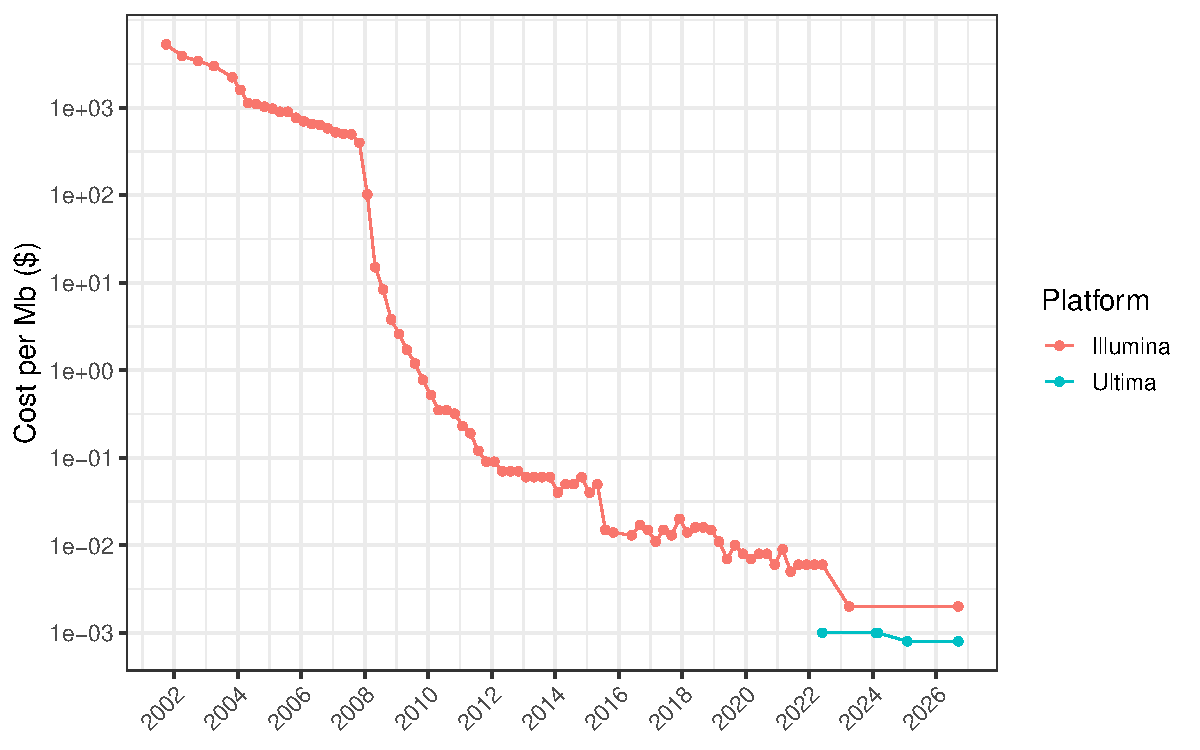
\includegraphics[width=0.75\linewidth]{slides/sequencing_cost.pdf}
  \caption{Cost per megabase of DNA sequence over time. The steep drop around 2008 corresponds to the arrival of second-generation (short-read) sequencing. The first human genome (Human Genome Project) cost roughly \$3 billion; later milestones are the ``\$1000 genome'' and the ``\$100 genome''. Data from the NHGRI Genome Sequencing Program~\citep{wetterstrand} and Ultima Genomics announcements.}
  \label{fig:seqcost}
\end{figure}

\subsection{DNA sequencing}

Sequencing was first used to read genomes, either of different species or of different individuals of the same species (usually humans). Comparing the genomes of species is the domain of \emph{comparative genomics}. Regions that are conserved across species are likely to be functionally important, and differences between, for example, human and chimpanzee genomes inform the study of evolution. Comparing the genomes of individuals underpins \emph{population genetics}, which studies how genetic variation in a population arises and changes through bottlenecks, migration and selection, and \emph{statistical genetics}, which relates genetic variation to traits.

\subsection{Statistical genetics}

Statistical genetics asks how genotype (an individual's genetic make-up) is associated with phenotype (a trait), and ideally which of those associations are causal. The trait might be quantitative, like height, or a disease. For example, people carry different versions (\emph{alleles}) of the gene \textit{APOE}, and these alleles confer different risks of Alzheimer's disease. More generally we want to know which genetic differences, and which genes, contribute to a phenotype. That knowledge can guide the design of drugs that intervene on the relevant genes, or the breeding and engineering of crops that are more resilient to climate change.

One motivation for genome-wide association studies (GWAS) comes from retrospective analyses of drug development. Drug targets that are supported by human genetic evidence are at least twice as likely to progress from clinical trials to approval as targets without such support (Figure~\ref{fig:genetic_support}). The genetic evidence can come from Mendelian disease genes, catalogued in Online Mendelian Inheritance in Man (OMIM), or from GWAS, where linking an associated variant to a gene requires additional information such as linkage disequilibrium, expression quantitative trait loci (eQTLs) and enhancer-gene maps.

\begin{figure}[t]
  \centering
  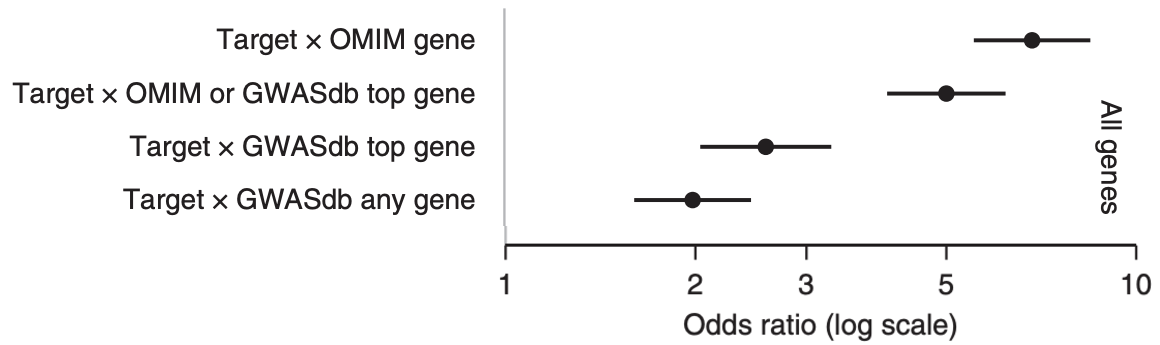
\includegraphics[width=0.75\linewidth]{slides/genetic_support_odds_ratio.png}
  \caption{Odds ratio of a drug target-indication pair progressing through clinical development when the target gene has genetic support for the indication, by source of genetic evidence. OMIM, Online Mendelian Inheritance in Man; GWASdb, a database of genome-wide association study results. Reproduced from \citet{nelson2015}; see \citet{king2019} for revised estimates.}
  \label{fig:genetic_support}
\end{figure}

\subsection{Functional genomics}

Functional genomics uses sequencing for a different task, measuring the state of cells or tissue samples. ``Functional'' refers to using these measurements to understand how cells and genes function, that is, how they carry out the processes they need to survive and respond to their environment. The typical workflow is shown in Figure~\ref{fig:fg_loop}. We take a sample of cells, from an experiment or a patient, and use biochemistry to convert the quantity we want to measure into DNA molecules. We then sequence that DNA. The computational task is to infer the original state of the cells from the sequencing reads.

\begin{figure}[t]
  \centering
  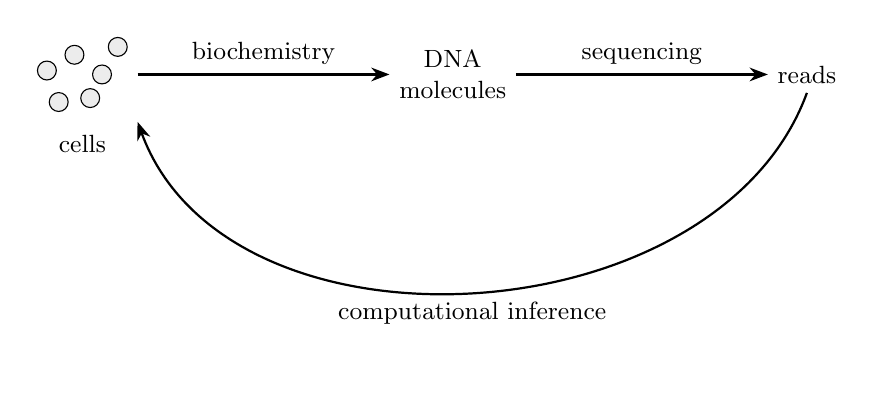
\begin{tikzpicture}[>=Stealth, node distance=3.2cm, every node/.style={font=\small}]
    \node (cells) {
      \tikz{\foreach \x/\y in {0/0,0.35/0.2,0.7/-0.05,0.15/-0.4,0.55/-0.35,0.9/0.3}
              \draw[fill=gray!15] (\x,\y) circle (0.12);}
    };
    \node[below=0.05cm of cells] {cells};
    \node[right=of cells, align=center] (dna) {DNA\\molecules};
    \node[right=of dna] (reads) {reads};
    \draw[->, thick] (cells) -- node[above, align=center] {biochemistry} (dna);
    \draw[->, thick] (dna) -- node[above] {sequencing} (reads);
    \draw[->, thick] (reads.south) to[out=-110, in=-70] node[below] {computational inference} (cells.south east);
  \end{tikzpicture}
  \caption{The functional genomics workflow. A molecular quantity of interest in a sample of cells is converted to DNA, the DNA is sequenced, and computational methods infer the state of the cells from the reads.}
  \label{fig:fg_loop}
\end{figure}

%======================================================================
\section{A molecular biology primer}
%======================================================================

\subsection{The central dogma}

The central dogma of molecular biology describes the flow of information in a cell. DNA, the long-term information store, is \emph{transcribed} into RNA, which mostly acts as an intermediate ``messenger''. RNA is then \emph{translated} into protein, the worker molecules of the cell, such as enzymes and structural proteins. The three molecules differ in abundance (Table~\ref{tab:central_dogma}). A human cell typically has two copies of its DNA, one inherited from each parent, while the number of RNA and protein copies of a given gene ranges from zero to tens or thousands.

\begin{table}[t]
  \centering
  \caption{The central dogma and typical copy numbers per cell for one gene. RNA and protein counts vary widely between genes and cell types; the values are orders of magnitude.}
  \label{tab:central_dogma}
  \begin{tabular}{lll}
    \toprule
    Molecule & Role & Copies per cell \\
    \midrule
    DNA & long-term information store & 2 \\
    \quad $\downarrow$ transcription & & \\
    RNA & intermediate (messenger) & 0--30 \\
    \quad $\downarrow$ translation & & \\
    Protein & ``worker'' molecules, e.g.\ enzymes, structural & 0--$10^4$ \\
    \bottomrule
  \end{tabular}
\end{table}

\subsection{Genomes, chromosomes and genes}

The genome is divided into chromosomes, each a long DNA molecule; a human chromosome is of the order of $10^8$ base pairs long. Genes are the segments of a chromosome that are transcribed, and the stretches between them are \emph{intergenic} regions (Figure~\ref{fig:cell}). In a eukaryotic cell the chromosomes are held in the nucleus. When a gene is expressed, it is transcribed into RNA molecules in the nucleus, typically of the order of 1000 nucleotides (nt) long. The RNA is exported to the cytoplasm, where it is translated into protein. Some proteins return to the nucleus and regulate the transcription of other genes, which closes a feedback loop that we will meet again when we study gene regulation.

\begin{figure}[t]
  \centering
  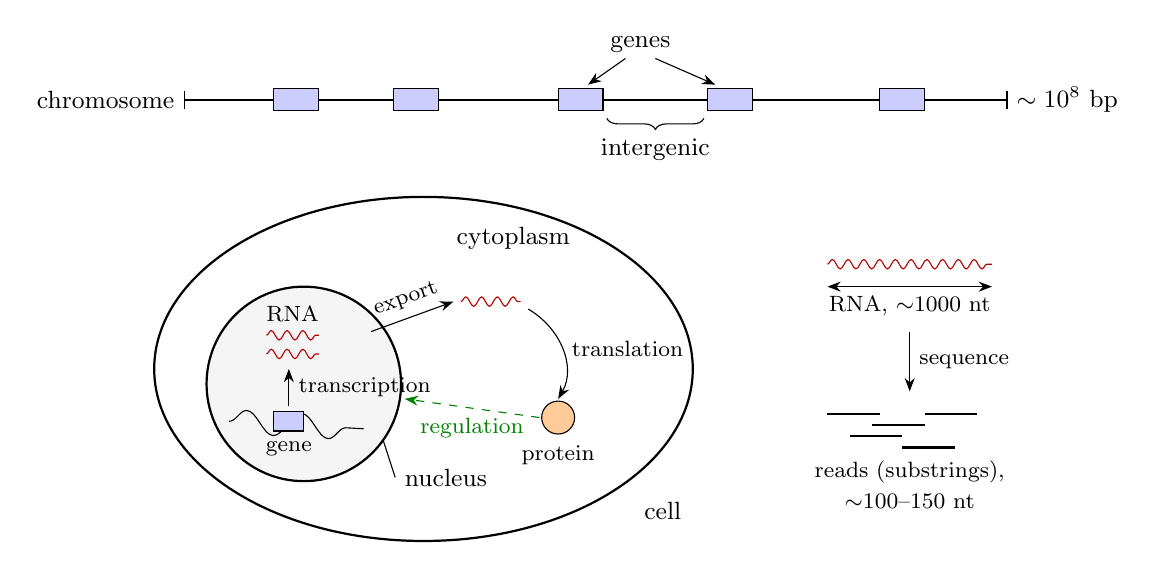
\begin{tikzpicture}[>=Stealth, every node/.style={font=\small}, scale=0.95]
    % chromosome with genes
    \draw[thick] (0,0) -- (11,0);
    \draw (0,-0.12) -- (0,0.12); \draw (11,-0.12) -- (11,0.12);
    \foreach \x in {1.2, 2.8, 5.0, 7.0, 9.3}
      \draw[fill=blue!20] (\x,-0.15) rectangle (\x+0.6,0.15);
    \node[left] at (0,0) {chromosome};
    \node[above] at (6.1,0.5) {genes};
    \draw[->] (5.9,0.55) -- (5.4,0.2);
    \draw[->] (6.3,0.55) -- (7.1,0.2);
    \draw[decorate, decoration={brace, mirror, amplitude=4pt}] (5.65,-0.25) -- (6.95,-0.25)
      node[midway, below=4pt] {intergenic};
    \node[right] at (11,0) {$\sim 10^8$ bp};
    % cell
    \begin{scope}[yshift=-3.6cm]
      \draw[thick] (3.2,0) ellipse (3.6cm and 2.3cm);
      \draw[thick, fill=gray!8] (1.6,-0.2) circle (1.3cm);
      \node (nuc) at (3.5,-1.45) {nucleus};
      \draw (nuc.west) -- (2.66,-0.95);
      \node at (4.4,1.75) {cytoplasm};
      \node at (6.4,-1.9) {cell};
      \draw[decorate, decoration={snake, amplitude=1.5mm, segment length=7mm}] (0.6,-0.7) -- (2.4,-0.8);
      \draw[fill=blue!20] (1.2,-0.83) rectangle (1.6,-0.57);
      \node[below] at (1.4,-0.85) {\footnotesize gene};
      \draw[->] (1.4,-0.5) -- (1.4,0.0) node[midway, right] {\footnotesize transcription};
      \draw[decorate, decoration={snake, amplitude=0.6mm, segment length=2mm}, red!70!black] (1.1,0.2) -- (1.8,0.2);
      \draw[decorate, decoration={snake, amplitude=0.6mm, segment length=2mm}, red!70!black] (1.1,0.45) -- (1.8,0.45);
      \node[above] at (1.45,0.5) {\footnotesize RNA};
      \draw[->] (2.5,0.5) -- (3.6,0.9) node[midway, above, sloped] {\footnotesize export};
      \draw[decorate, decoration={snake, amplitude=0.6mm, segment length=2mm}, red!70!black] (3.7,0.9) -- (4.5,0.9);
      \draw[->] (4.6,0.8) to[out=-30, in=60] node[right] {\footnotesize translation} (5.0,-0.4);
      \draw[fill=orange!40] (5.0,-0.65) circle (0.22);
      \node[below] at (5.0,-0.9) {\footnotesize protein};
      \draw[->, dashed, green!50!black] (4.75,-0.65) -- (2.95,-0.4) node[midway, below] {\footnotesize regulation};
    \end{scope}
    % RNA and reads
    \begin{scope}[xshift=8.6cm, yshift=-2.2cm]
      \draw[red!70!black, decorate, decoration={snake, amplitude=0.6mm, segment length=2mm}] (0,0) -- (2.2,0);
      \draw[<->] (0,-0.3) -- (2.2,-0.3) node[midway, below] {\footnotesize RNA, $\sim$1000 nt};
      \draw[->] (1.1,-0.9) -- (1.1,-1.7) node[midway, right] {\footnotesize sequence};
      \foreach \x/\y in {0/-2.0, 0.6/-2.15, 1.3/-2.0, 0.3/-2.3, 1.0/-2.45}
        \draw[thick] (\x,\y) -- (\x+0.7,\y);
      \node[below, align=center] at (1.1,-2.5) {\footnotesize reads (substrings),\\ \footnotesize $\sim$100--150 nt};
    \end{scope}
  \end{tikzpicture}
  \caption{Genes are segments of chromosomes separated by intergenic regions (top). In the nucleus a gene is transcribed into RNA, which is exported to the cytoplasm and translated into protein; some proteins feed back to regulate transcription (bottom). Sequencing RNA produces reads that are short substrings of the RNA molecules (right).}
  \label{fig:cell}
\end{figure}

\subsection{DNA}

DNA is a double-stranded polymer of four nucleotides, A, T, G and C. The two strands are complementary: A pairs with T and C pairs with G (Figure~\ref{fig:dna}). Each strand has a direction, written from its $5'$ end to its $3'$ end, and the two strands run in opposite directions. By convention we call one strand the forward ($+$) strand and the other the reverse ($-$) strand, so that a sequence read from the reverse strand is the reverse complement of the forward sequence. Separating the strands is the first step both in duplicating DNA, during mitosis (asexual cell division) and meiosis (the cell division that produces gametes for sexual reproduction), and in transcription.

\begin{figure}[t]
  \centering
  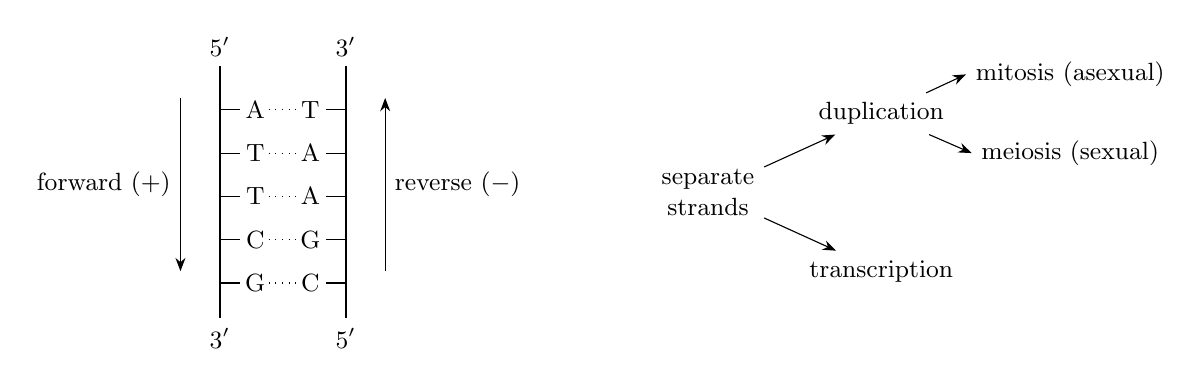
\begin{tikzpicture}[>=Stealth, every node/.style={font=\small}]
    \draw[thick] (0,0) -- (0,-3.2); \draw[thick] (1.6,0) -- (1.6,-3.2);
    \node[above] at (0,0) {$5'$}; \node[below] at (0,-3.2) {$3'$};
    \node[above] at (1.6,0) {$3'$}; \node[below] at (1.6,-3.2) {$5'$};
    \foreach \a/\b [count=\i] in {A/T, T/A, T/A, C/G, G/C} {
      \draw (0,-0.55*\i) -- (0.25,-0.55*\i); \draw (1.35,-0.55*\i) -- (1.6,-0.55*\i);
      \node at (0.45,-0.55*\i) {\a}; \node at (1.15,-0.55*\i) {\b};
      \draw[dotted] (0.62,-0.55*\i) -- (0.98,-0.55*\i);
    }
    \draw[->] (-0.5,-0.4) -- (-0.5,-2.6) node[midway, left] {forward ($+$)};
    \draw[->] (2.1,-2.6) -- (2.1,-0.4) node[midway, right] {reverse ($-$)};
    % fate of separated strands
    \node[align=center] (sep) at (6.2,-1.6) {separate\\strands};
    \node (dup) at (8.4,-0.6) {duplication};
    \node (tx) at (8.4,-2.6) {transcription};
    \node[align=left] (mit) at (10.8,-0.1) {mitosis (asexual)};
    \node[align=left] (mei) at (10.8,-1.1) {meiosis (sexual)};
    \draw[->] (sep) -- (dup); \draw[->] (sep) -- (tx);
    \draw[->] (dup) -- (mit.west); \draw[->] (dup) -- (mei.west);
  \end{tikzpicture}
  \caption{DNA is a double-stranded polymer. The strands are complementary (A--T, C--G) and antiparallel. Strand separation is required for duplication and for transcription.}
  \label{fig:dna}
\end{figure}

\subsection{RNA and gene expression}

RNA uses the same nucleotides as DNA except that thymine (T) is replaced by uracil (U). The number of RNA copies of a gene in a cell is what we call that gene's \emph{expression}. Cells control expression in response to three kinds of question: \emph{when} (for example at different stages of development), \emph{where} (in which tissues and cell types) and \emph{why} (in response to a stimulus, for example an immune challenge). The mechanisms by which they do so are collectively called \emph{gene regulation}.

\subsection{RNA-seq}

RNA sequencing (RNA-seq) measures gene expression (Figure~\ref{fig:rnaseq}). RNA molecules are extracted from cells; they are typically of the order of 1000 nt long. The RNA is fragmented and reverse transcribed into complementary DNA (cDNA), giving fragments of around 300--400 nt. The cDNA is sequenced, producing reads of around 100--150 nt; a typical experiment yields 30--100 million reads per sample. The reads are aligned to the genome, and the number of reads overlapping each gene is counted. These counts, suitably normalized, are the gene expression measurements we will model.

\begin{figure}[t]
  \centering
  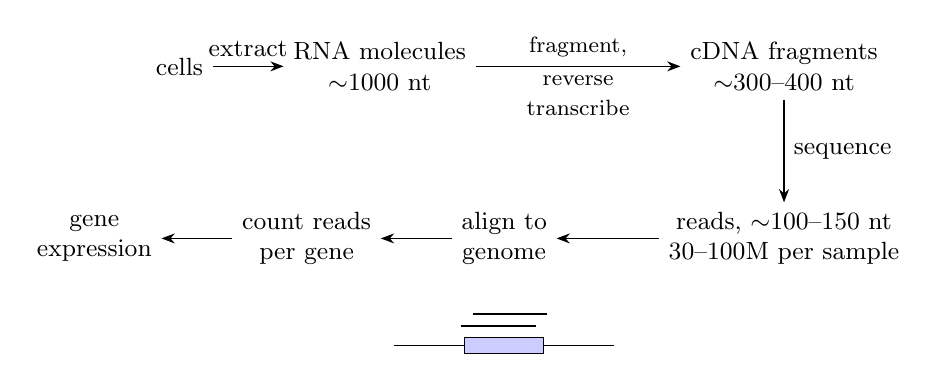
\begin{tikzpicture}[>=Stealth, node distance=0.9cm, every node/.style={font=\small, align=center}]
    \node (cells) {cells};
    \node[right=of cells] (rna) {RNA molecules\\$\sim$1000 nt};
    \node[right=2.6cm of rna] (cdna) {cDNA fragments\\$\sim$300--400 nt};
    \node[below=1.3cm of cdna] (reads) {reads, $\sim$100--150 nt\\30--100M per sample};
    \node[left=1.3cm of reads] (align) {align to\\genome};
    \node[left=of align] (count) {count reads\\per gene};
    \node[left=of count] (expr) {gene\\expression};
    \draw[->] (cells) -- node[above] {extract} (rna);
    \draw[->] (rna) -- node[above, font=\footnotesize] {fragment,} node[below, font=\footnotesize] {reverse} node[below=0.3cm, font=\footnotesize] {transcribe} (cdna);
    \draw[->] (cdna) -- node[right] {sequence} (reads);
    \draw[->] (reads) -- (align);
    \draw[->] (align) -- (count);
    \draw[->] (count) -- (expr);
    % reads piling up on a gene
    \begin{scope}[shift={($(align.south)+(-1.4,-0.9)$)}]
      \draw (0,0) -- (2.8,0);
      \draw[fill=blue!20] (0.9,-0.1) rectangle (1.9,0.1);
      \foreach \x/\y in {0.85/0.25, 1.15/0.25, 1.45/0.25, 1.0/0.4, 1.3/0.4, 1.6/0.4}
        \draw[thick] (\x,\y) -- (\x+0.35,\y);
    \end{scope}
  \end{tikzpicture}
  \caption{The RNA-seq workflow. Read counts per gene, after normalization, are used as measurements of gene expression.}
  \label{fig:rnaseq}
\end{figure}

Bulk RNA-seq is applied to a tissue sample containing many cells, so it measures the average expression across all cells in the sample. Single-cell RNA-seq (scRNA-seq) measures expression in individual cells, which reveals heterogeneity between cell types that bulk measurements average over (Figure~\ref{fig:bulk_sc}). We will return to single-cell data in later chapters.

\begin{figure}[t]
  \centering
  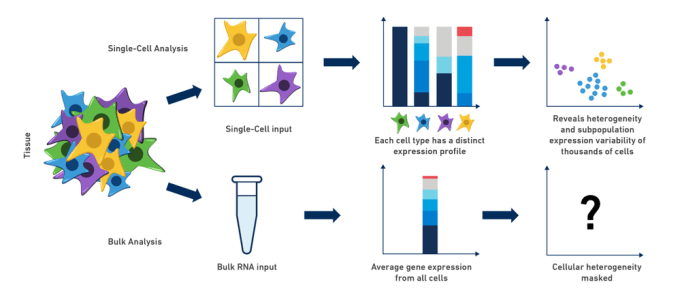
\includegraphics[width=0.85\linewidth]{slides/bulk_vs_singlecell.png}
  \caption{Bulk RNA-seq measures the average expression across all cells in a sample, masking differences between cell types. Single-cell RNA-seq measures each cell separately and can reveal subpopulations. Reproduced from \citet{tenx_blog}.}
  \label{fig:bulk_sc}
\end{figure}

%======================================================================
\section{Application: predicting cancer drug sensitivity}
\label{sec:drug_app}
%======================================================================

Cancer cell lines are populations of cells derived from patient tumours that can be grown in culture indefinitely (Figure~\ref{fig:culture}). Each line can be profiled with RNA-seq and other assays, and in parallel screened for its sensitivity to a panel of drugs. Several consortia have generated such data at scale, including the Cancer Cell Line Encyclopedia (CCLE)~\citep{barretina2012}, Genomics of Drug Sensitivity in Cancer (GDSC)~\citep{garnett2012} and the Cancer Therapeutics Response Portal (CTRP)~\citep{seashore2015}. The resulting data can be arranged as two matrices with a shared row index (Figure~\ref{fig:data_matrices}a). The expression matrix has one row per cell line and one column per gene. The sensitivity matrix has one row per cell line and one column per drug. Predicting the sensitivity of cell lines to one drug, say drug A, from their gene expression is a regression problem, and it is the running example of the first half of this chapter.

\begin{figure}[t]
  \centering
  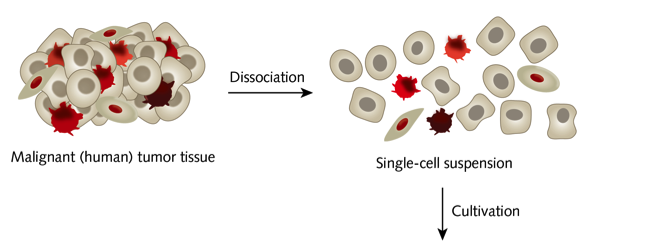
\includegraphics[width=0.5\linewidth]{slides/primary_culture.png}
  \caption{Deriving a primary cancer cell culture from tumour tissue: dissociation into single cells, cultivation, and depletion of non-malignant cells. The resulting lines can be profiled (e.g.\ by RNA-seq) and screened for drug sensitivity. \textbf{[Source to be confirmed.]}}
  \label{fig:culture}
\end{figure}

\begin{figure}[t]
  \centering
  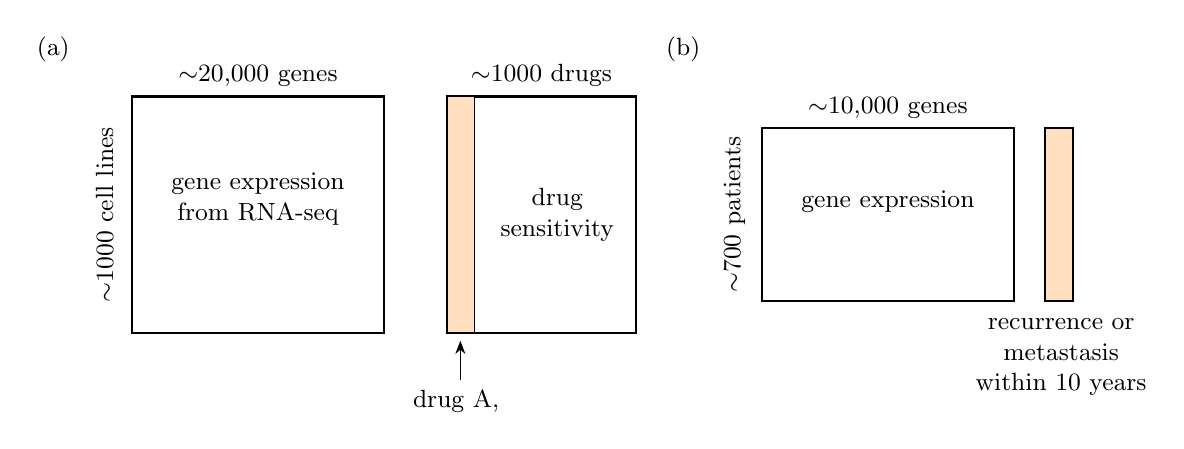
\begin{tikzpicture}[>=Stealth, every node/.style={font=\small, align=center}]
    \node at (-1.0,3.6) {(a)};
    \draw[thick] (0,0) rectangle (3.2,3.0);
    \node at (1.6,1.5) {gene expression\\from RNA-seq\\[2pt] $\mX$};
    \node[above] at (1.6,3.0) {$\sim$20{,}000 genes};
    \node[rotate=90] at (-0.35,1.5) {$\sim$1000 cell lines};
    \draw[thick] (4.0,0) rectangle (6.4,3.0);
    \draw[fill=orange!25] (4.0,0) rectangle (4.35,3.0);
    \node at (5.4,1.5) {drug\\sensitivity};
    \node[above] at (5.2,3.0) {$\sim$1000 drugs};
    \draw[<-] (4.17,-0.1) -- (4.17,-0.6) node[below] {drug A, $\vy$};
    % Oncotype DX
    \begin{scope}[xshift=8.0cm]
      \node at (-1.0,3.6) {(b)};
      \draw[thick] (0,0.4) rectangle (3.2,2.6);
      \node at (1.6,1.5) {gene expression\\$\mX$};
      \node[above] at (1.6,2.6) {$\sim$10{,}000 genes};
      \node[rotate=90] at (-0.35,1.5) {$\sim$700 patients};
      \draw[thick, fill=orange!25] (3.6,0.4) rectangle (3.95,2.6);
      \node[right] at (4.0,1.5) {$\vy$};
      \node[below, align=center] at (3.8,0.3) {recurrence or\\metastasis\\within 10 years};
    \end{scope}
  \end{tikzpicture}
  \caption{Data matrices for the two applications in this chapter. (a) Cancer cell line drug screens: an expression matrix $\mX$ (cell lines $\times$ genes) and a sensitivity matrix (cell lines $\times$ drugs). Predicting one column $\vy$ of the sensitivity matrix from $\mX$ is a regression problem. (b) Predicting breast cancer recurrence from tumour gene expression (Section~\ref{sec:classification}) is a binary classification problem.}
  \label{fig:data_matrices}
\end{figure}

Sensitivity is summarized from a dose-response experiment for each drug-cell line pair (Figure~\ref{fig:dose_response}). The cell line is grown at a series of drug concentrations and its growth is measured relative to untreated cells. Two common summaries are the IC$_{50}$, the concentration at which growth is reduced by half, and the \emph{activity area}, the area between the dose-response curve and 100\% growth. A larger activity area means a more sensitive cell line. The CCLE study, for example, screened 24 drugs across 479 cell lines spanning many tumour types (Figure~\ref{fig:ccle_types})~\citep{barretina2012}.

\begin{figure}[t]
  \centering
  \begin{subfigure}[b]{0.48\linewidth}
    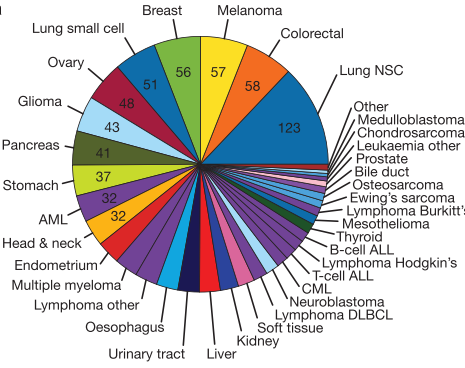
\includegraphics[width=\linewidth]{slides/ccle_tumour_types.png}
    \caption{}
    \label{fig:ccle_types}
  \end{subfigure}\hfill
  \begin{subfigure}[b]{0.48\linewidth}
    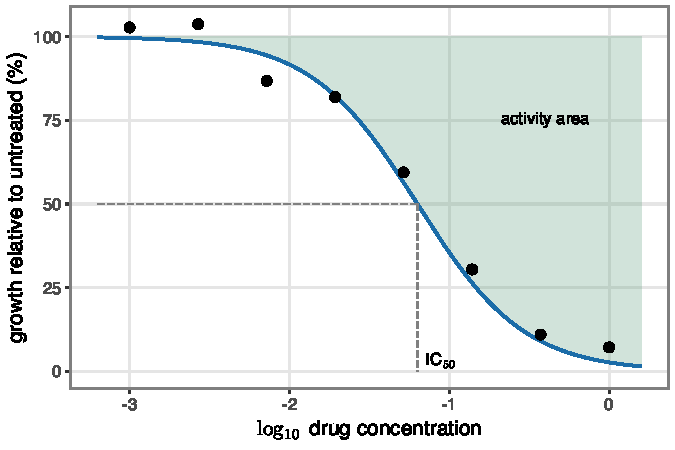
\includegraphics[width=\linewidth]{dose_response.pdf}
    \caption{}
    \label{fig:dose_response}
  \end{subfigure}
  \caption{(a) Number of cell lines by tumour type in the CCLE drug screen, reproduced from \citet{barretina2012}. (b) Schematic dose-response curve for a single drug-cell line pair. The IC$_{50}$ is the concentration at which growth falls to 50\% of untreated; the activity area (shaded) is the area between the curve and 100\% growth.}
\end{figure}

%======================================================================
\section{Linear regression}
\label{sec:linreg}
%======================================================================

Linear regression models a continuous \emph{response} (also called the dependent variable or output), such as drug sensitivity, as a linear function of one or more \emph{inputs} (features, independent variables, covariates), such as gene expression levels (Figure~\ref{fig:linreg}).

\begin{figure}[t]
  \centering
  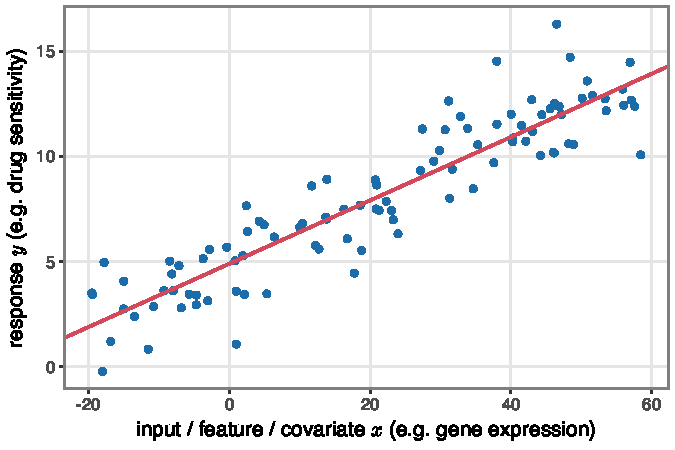
\includegraphics[width=0.6\linewidth]{linreg_scatter.pdf}
  \caption{Linear regression with one covariate. Each point is a sample; the line is the least-squares fit.}
  \label{fig:linreg}
\end{figure}

\subsection{The model}

Let $N$ be the number of samples (cell lines) and $P$ the number of features (genes). We index samples by $i\in\{1,\dots,N\}$ and features by $j\in\{1,\dots,P\}$. Let $y_i\in\R$ be the response of sample $i$, $X_{ij}\in\R$ the expression of gene $j$ in sample $i$, $\beta_j\in\R$ the coefficient of gene $j$, and $\epsilon_i\in\R$ a noise term. The linear regression model is
\begin{equation}
  y_i = \sum_{j=1}^P X_{ij}\beta_j + \epsilon_i + \mu ,
  \label{eq:linreg_scalar}
\end{equation}
where $\mu$ is an intercept. A coefficient $\beta_j=0$ means gene $j$ has no effect on the response; $\beta_j<0$ means higher expression of gene $j$ is associated with lower sensitivity. We will usually assume $\vy$ has been centered (mean zero), so that $\mu=0$, or equivalently absorb the intercept into $\vb$ by appending a column of ones to the features. The responses and features are observed; the coefficients are the unknowns we want to estimate; the noise is a nuisance.

In vector notation, let $\vx_i\in\R^{P}$ be the features of sample $i$ (as a column vector) and $\vb\in\R^P$ the coefficient vector. Then $y_i = \vx_i^\top\vb + \epsilon_i$, where $\vx_i^\top$ is $1\times P$ and $\vb$ is $P\times 1$, so their inner product is a scalar. Stacking samples, let $\vy\in\R^N$, let $\mX\in\R^{N\times P}$ be the matrix whose $i$-th row is $\vx_i^\top$, and let $\veps\in\R^N$. The model is
\begin{equation}
  \underbrace{\vy}_{N\times 1} = \underbrace{\mX}_{N\times P}\;\underbrace{\vb}_{P\times 1} + \underbrace{\veps}_{N\times 1}, \qquad \epsilon_i \overset{\text{iid}}{\sim} \Normal(0,\sigma^2),
  \label{eq:linreg}
\end{equation}
where $\sigma^2$ is the noise variance and ``iid'' means independent and identically distributed. We write $\mX_{:j}\in\R^N$ for the $j$-th column of $\mX$, the expression of gene $j$ across samples.

\subsection{Likelihood}

The likelihood is the probability of the observed data as a function of the parameters, $L(\vb)=p(\mathcal{D}\mid\vb)=p(\vy\mid\mX,\vb)$, where $\mathcal{D}$ denotes the data. Since $\epsilon_i=y_i-\vx_i^\top\vb$ is Gaussian, the likelihood of one sample is
\begin{equation}
  p(y_i\mid\vx_i,\vb) = \frac{1}{\sqrt{2\pi\sigma^2}}\exp\left(-\frac{1}{2\sigma^2}(y_i-\vx_i^\top\vb)^2\right).
\end{equation}
Because the noise terms are independent, the likelihood of all samples is the product
\begin{equation}
  p(\vy\mid\mX,\vb) = \prod_{i=1}^N p(y_i\mid\vx_i,\vb) = \frac{1}{(2\pi\sigma^2)^{N/2}}\exp\left(-\frac{1}{2\sigma^2}\sum_{i=1}^N(y_i-\vx_i^\top\vb)^2\right),
\end{equation}
and the log likelihood is
\begin{equation}
  \log L(\vb) = -\frac{N}{2}\log 2\pi\sigma^2 - \frac{1}{2\sigma^2}\sum_{i=1}^N\left(y_i-\vx_i^\top\vb\right)^2 .
  \label{eq:loglik}
\end{equation}
The first term does not depend on $\vb$, so maximizing the log likelihood over $\vb$ is equivalent to minimizing the sum of squared errors $\sum_i(y_i-\vx_i^\top\vb)^2$.

\subsection{Finding the optimal parameters}

The log likelihood~\eqref{eq:loglik} is a concave quadratic in $\vb$, so its maximum is where the gradient is zero,
\begin{equation}
  \nabla_{\vb}\log L = \frac{1}{\sigma^2}\sum_{i=1}^N \vx_i\left(y_i-\vx_i^\top\vb\right) = 0
  \quad\Rightarrow\quad
  \sum_{i=1}^N \vx_i\vx_i^\top\vb = \sum_{i=1}^N\vx_i y_i .
\end{equation}
In matrix notation this is $\mX^\top\mX\vb = \mX^\top\vy$, with dimensions $[P\times N][N\times P][P\times 1]=[P\times N][N\times 1]$. Solving gives the maximum likelihood estimate (MLE), also known as the ordinary least squares (OLS) estimate,
\begin{equation}
  \hat\vb = (\mX^\top\mX)^{-1}\mX^\top\vy .
  \label{eq:ols}
\end{equation}
In practice we do not form the inverse explicitly. Equation~\eqref{eq:ols} has the form $\mathbf{A}\vb=\mathbf{c}$ with $\mathbf{A}=\mX^\top\mX$ and $\mathbf{c}=\mX^\top\vy$, so we call a linear solver, $\hat\vb=\texttt{solve}(\mX^\top\mX,\mX^\top\vy)$, which is faster and numerically more stable.

\subsection{Special case: independent covariates}

Suppose $\vy$ and each column $\mX_{:j}$ have been standardized to mean zero and variance one, and that the features are uncorrelated, $\operatorname{corr}(\mX_{:j},\mX_{:k})=0$ for $j\neq k$. Then $\mX^\top\mX=N\mI$, where $\mI$ is the $P\times P$ identity, and
\begin{equation}
  \hat\vb = (N\mI)^{-1}\mX^\top\vy = \frac{1}{N}\mX^\top\vy, \qquad \hat\beta_j = \frac{1}{N}\mX_{:j}^\top\vy = \operatorname{corr}(\mX_{:j},\vy).
\end{equation}
When features are uncorrelated, the regression coefficient of gene $j$ is the correlation between its expression and the response, and each gene can be considered separately. When features are correlated, as genes usually are, the coefficients must be estimated jointly.

\subsection{\texorpdfstring{Small $N$, large $P$}{Small N, large P} and colinearity}

Genomic data sets often have more features than samples: thousands of genes but hundreds of cell lines. Since $\operatorname{rank}(\mX^\top\mX)\leq\min(N,P)$, when $N<P$ the $P\times P$ matrix $\mX^\top\mX$ is not invertible and~\eqref{eq:ols} has no unique solution. The columns of $\mX$ are then linearly dependent, a situation called \emph{colinearity}: some combination of features can be changed without changing the predictions, and the likelihood is flat along that direction.

Even when $N>P$, strongly correlated features make the problem \emph{poorly conditioned}. The condition number of $\mX^\top\mX$ is the ratio of its largest to smallest eigenvalue, $\kappa=\nu_{\max}/\nu_{\min}$. A large condition number means $\mX^\top\mX$ is close to non-invertible, and small changes to the data produce large changes in $\hat\vb$. Figure~\ref{fig:colinearity} (left) shows the sum of squares for two features with correlation $0.98$. The contours are elongated along the direction $\beta_1+\beta_2=\text{const}$: if $\vx_1\approx\vx_2$, increasing $\beta_1$ and decreasing $\beta_2$ by the same amount leaves the fit nearly unchanged, so all points along this ridge are almost equally good. Adding a penalty on the size of $\vb$ (right) makes the minimum well defined. The next section motivates such penalties.

\begin{figure}[t]
  \centering
  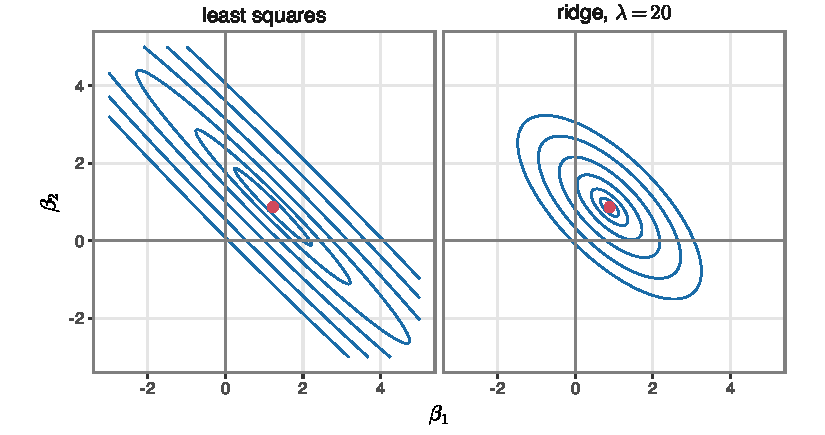
\includegraphics[width=0.85\linewidth]{colinearity_contours.pdf}
  \caption{Contours of the sum of squares $\sum_i(y_i-\vx_i^\top\vb)^2$ for two features with correlation $0.98$ (left) and of the ridge objective, which adds $\lambda\|\vb\|_2^2$ (right). The least-squares minimum lies in a long, flat valley and is unstable; the ridge minimum is well defined. Red points mark the minimizers.}
  \label{fig:colinearity}
\end{figure}

%======================================================================
\section{Priors, Bayes' rule and ridge regression}
\label{sec:ridge}
%======================================================================

\subsection{Bayes' rule}

For parameters $\theta$ and data $\mathcal{D}$, Bayes' rule is
\begin{equation}
  \underbrace{p(\theta\mid\mathcal{D})}_{\text{posterior}} = \frac{\overbrace{p(\mathcal{D}\mid\theta)}^{\text{likelihood}}\;\overbrace{p(\theta)}^{\text{prior}}}{\underbrace{p(\mathcal{D})}_{\text{evidence}}} ,
\end{equation}
where the evidence or \emph{marginal likelihood} $p(\mathcal{D})=\int p(\mathcal{D}\mid\theta)p(\theta)\,d\theta$ does not depend on $\theta$. For linear regression, $\mathcal{D}=\vy$ (we condition on $\mX$ throughout) and $\theta=\vb$.

A natural prior expresses the belief that most coefficients are small: each coefficient is drawn independently from a Gaussian with mean zero and variance $\sigma_\beta^2$,
\begin{equation}
  \beta_j\overset{\text{iid}}{\sim}\Normal(0,\sigma_\beta^2), \qquad p(\beta_j)=\Normal(\beta_j\mid 0,\sigma^2_\beta)=\frac{1}{\sqrt{2\pi\sigma_\beta^2}}\exp\left(-\frac{\beta_j^2}{2\sigma_\beta^2}\right).
\end{equation}
Figure~\ref{fig:prior_post} shows the prior, likelihood and posterior for a single coefficient. The posterior combines the two sources of information and is more concentrated than either.

\begin{figure}[t]
  \centering
  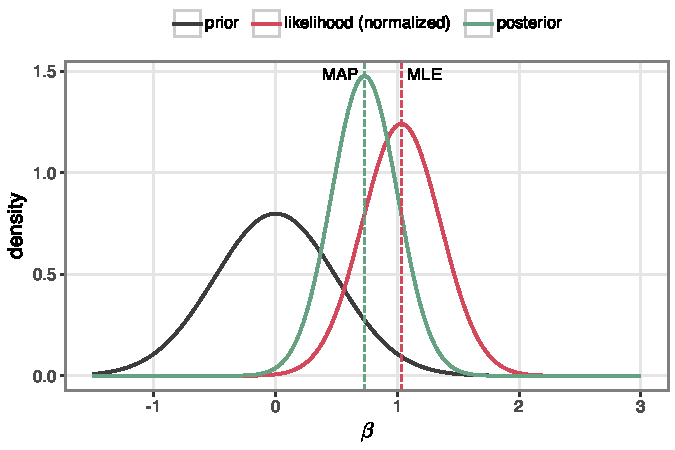
\includegraphics[width=0.6\linewidth]{prior_likelihood_posterior.pdf}
  \caption{Prior, likelihood (normalized to integrate to one) and posterior for a single regression coefficient with $N=5$ samples. The posterior mode (MAP) is shrunk from the maximum likelihood estimate (MLE) toward the prior mean of zero.}
  \label{fig:prior_post}
\end{figure}

\subsection{Maximum a posteriori estimation is L2 regularization}

Taking logs of Bayes' rule,
\begin{align}
  \log p(\vb\mid\vy) &= \log p(\vy\mid\mX,\vb) + \log p(\vb) - \log p(\vy) \nonumber\\
  &= -\frac{1}{2\sigma^2}\sum_{i=1}^N\left(y_i-\vx_i^\top\vb\right)^2 - \frac{1}{2\sigma_\beta^2}\sum_{j=1}^P\beta_j^2 + \text{const},
  \label{eq:logpost}
\end{align}
where the constant collects $\log p(\vy)$ and the normalizing terms $-\frac{N}{2}\log 2\pi\sigma^2-\frac{P}{2}\log 2\pi\sigma_\beta^2$, none of which depend on $\vb$. The maximum a posteriori (MAP) estimate maximizes~\eqref{eq:logpost}. Using $\nabla_{\vb}(\vb^\top\mathbf{A}\vb)=2\mathbf{A}\vb$ for symmetric $\mathbf{A}$, the gradient is
\begin{equation}
  \nabla_{\vb}\log p(\vb\mid\vy) = \frac{1}{\sigma^2}\sum_i\vx_i\left(y_i-\vx_i^\top\vb\right) - \frac{1}{\sigma_\beta^2}\vb = 0 .
\end{equation}
Rearranging, $\frac{1}{\sigma^2}\mX^\top\vy = \left(\frac{1}{\sigma^2}\mX^\top\mX + \frac{1}{\sigma_\beta^2}\mI\right)\vb$, and multiplying through by $\sigma^2$,
\begin{equation}
  \hat\vb_{\text{MAP}} = \left(\mX^\top\mX + \lambda\mI\right)^{-1}\mX^\top\vy, \qquad \lambda = \frac{\sigma^2}{\sigma^2_\beta}.
  \label{eq:ridge}
\end{equation}
This is the \emph{ridge regression} estimator~\citep{hoerl1970}. Equivalently, it minimizes the penalized loss
\begin{equation}
  \frac{1}{2}\sum_{i=1}^N\left(y_i-\vx_i^\top\vb\right)^2 + \frac{\lambda}{2}\|\vb\|_2^2 ,
\end{equation}
where $\|\vb\|_2^2=\sum_j\beta_j^2$. The added term is called \emph{L2 regularization}: it penalizes large coefficients and shrinks the estimate toward zero. Because $\lambda>0$ makes $\mX^\top\mX+\lambda\mI$ invertible for any $\mX$, ridge regression has a unique solution even when $N<P$. The regularization strength $\lambda$ is the ratio of noise variance to prior variance: a broad prior (large $\sigma_\beta^2$) or low noise means weak regularization. Only the ratio matters for $\hat\vb_{\text{MAP}}$. Scaling $\sigma^2$ and $\sigma_\beta^2$ together changes the curvature of the posterior, and therefore our uncertainty, but not its mode. Since the penalty treats all coefficients alike, features should be put on a common scale, usually by standardizing each column of $\mX$, before fitting.

Because the prior and likelihood are both Gaussian in $\vb$, the posterior is Gaussian as well, with mean $\hat\vb_{\text{MAP}}$ and covariance $\sigma^2(\mX^\top\mX+\lambda\mI)^{-1}$. For Gaussian posteriors the MAP and posterior mean coincide.

\subsection{\texorpdfstring{Choosing $\lambda$}{Choosing lambda}}

There are two common options for choosing the regularization strength.
\begin{enumerate}
  \item \emph{Cross-validation}: choose the $\lambda$ that gives the best predictions on held-out data (Section~\ref{sec:model_selection}).
  \item \emph{Empirical Bayes}, or maximum marginal likelihood: choose $\sigma^2$ and $\sigma^2_\beta$ to maximize the evidence $p(\vy\mid\mX,\sigma^2,\sigma_\beta^2)$. Integrating out $\vb$ gives $\vy\mid\mX\sim\Normal\left(\mathbf{0},\,\sigma_\beta^2\mX\mX^\top+\sigma^2\mI_N\right)$, which can be maximized numerically.
\end{enumerate}

Section 3.4.1 of \citet{esl} gives a complementary treatment of ridge regression.

%======================================================================
\section{Assessing regression performance}
\label{sec:regression_metrics}
%======================================================================

The metrics used for classification (accuracy, precision, recall, area under the ROC curve; Section~\ref{sec:classification_metrics}) do not apply directly to regression. If there is a natural threshold, one can binarize predictions and observations after fitting and then use classification metrics, but in general we want metrics designed for continuous outcomes. Let $\hat y_i=\vx_i^\top\hat\vb$ be the prediction for sample $i$.

\begin{itemize}
  \item The \emph{sum of squared errors} is $\text{SS}=\sum_i(y_i-\hat y_i)^2$. It is hard to interpret because it depends on the number of samples and on the scale of $y$.
  \item The \emph{mean squared error} $\text{MSE}=\frac{1}{N}\text{SS}$ removes the dependence on $N$, and the \emph{root mean squared error} $\text{RMSE}=\sqrt{\text{MSE}}$ is on the same scale, and in the same units, as $y$. MSE and RMSE estimate the noise variance $\sigma^2$ and standard deviation $\sigma$. This holds only if the model neither overfits, in which case they underestimate the noise, nor underfits, in which case they overestimate it.
  \item MSE and RMSE still depend on the scale of $y$, so they cannot be compared across data sets. The \emph{coefficient of determination} is
  \begin{equation}
    R^2 = 1-\frac{\text{SS}}{\text{TSS}} = 1-\frac{\text{MSE}}{s_y^2}, \qquad \text{TSS}=\sum_i(y_i-\bar y)^2,
  \end{equation}
  where $\bar y$ is the mean of $\vy$, $\text{TSS}$ is the total sum of squares and $s_y^2=\text{TSS}/N$ is the variance of the observations. For centered $\vy$, $\text{TSS}=\sum_i y_i^2$. $R^2$ is the proportion of variance explained (PVE) by the model. If $\vy$ is scaled to unit variance, $R^2=1-\text{MSE}$.
\end{itemize}

For the least-squares fit of a model with an intercept, evaluated on the training data, $R^2$ equals the squared Pearson correlation between $\vy$ and $\hat\vy$ and lies in $[0,1]$, with 0 meaning no agreement and 1 meaning perfect prediction. On held-out data the two can differ: the Pearson correlation ignores the mean and scale of the predictions, while $R^2$ does not, and held-out $R^2$ can be negative if predictions are worse than predicting the mean. Figure~\ref{fig:rmse} illustrates RMSE as the typical vertical distance of points from the fitted line.

\begin{figure}[t]
  \centering
  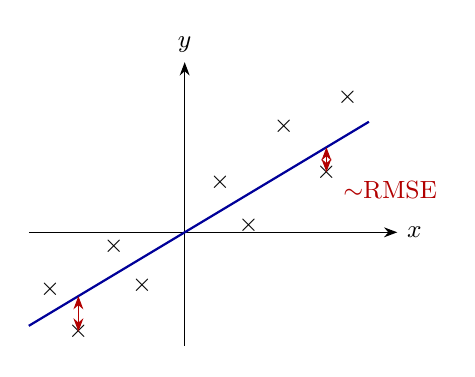
\begin{tikzpicture}[>=Stealth, every node/.style={font=\small}, scale=0.9]
    \draw[->] (-2.2,0) -- (3,0) node[right] {$x$};
    \draw[->] (0,-1.6) -- (0,2.4) node[above] {$y$};
    \draw[thick, blue!60!black] (-2.2,-1.32) -- (2.6,1.56);
    \foreach \x/\y in {-1.9/-0.8, -1.5/-1.4, -1.0/-0.2, -0.6/-0.75, 0.5/0.7, 0.9/0.1, 1.4/1.5, 2.0/0.85, 2.3/1.9}
      \node at (\x,\y) {$\times$};
    \draw[<->, red!70!black] (2.0,0.85) -- (2.0,1.2);
    \draw[<->, red!70!black] (-1.5,-1.4) -- (-1.5,-0.9);
    \node[right, red!70!black] at (2.1,0.6) {$\sim$RMSE};
  \end{tikzpicture}
  \caption{The RMSE is on the scale of the typical vertical deviation of observations from the fitted line.}
  \label{fig:rmse}
\end{figure}

A final summary is the statistical significance (p-value) of the Pearson or Spearman correlation between predictions and observations on held-out data. This is rarely reported in computer vision or natural language processing, but biological data are often noisy enough that $R^2$ is low and it is unclear whether we are predicting better than chance.

We sometimes describe a regression model informally as ``accurate''. For classification, accuracy has a specific meaning: the proportion of samples assigned to the correct class.

%======================================================================
\section{Model selection}
\label{sec:model_selection}
%======================================================================

\subsection{Training, validation and test sets}

To choose hyperparameters such as $\lambda$ and to assess how well a model generalizes, we split the samples into three sets (Figure~\ref{fig:splits}a). The \emph{training set} (for example 60\% of samples) is used in the likelihood or loss to fit the parameters $\vb$. The \emph{validation set} (20\%) is used to estimate the generalization error of models fit with different hyperparameters, and to pick the best. The \emph{test set} (20\%) is used once, at the end, for a final assessment of generalization. Using the test set to make modelling choices leads to optimistic estimates of performance.

\begin{figure}[t]
  \centering
  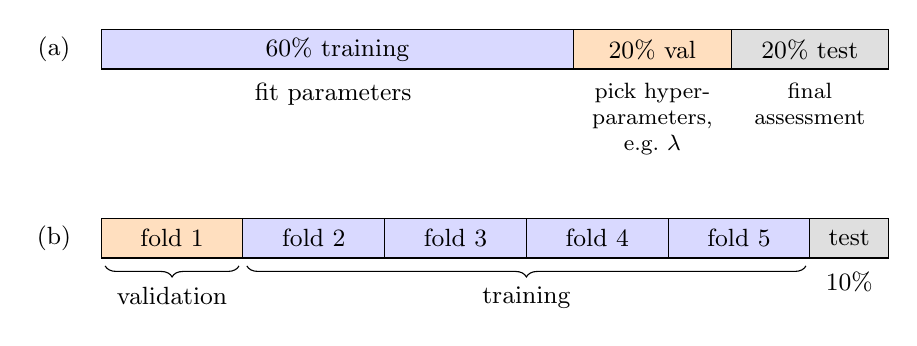
\begin{tikzpicture}[every node/.style={font=\small, align=center}]
    \node at (-0.6,0.25) {(a)};
    \draw[fill=blue!15] (0,0) rectangle (6,0.5); \node at (3,0.25) {60\% training};
    \draw[fill=orange!25] (6,0) rectangle (8,0.5); \node at (7,0.25) {20\% val};
    \draw[fill=gray!25] (8,0) rectangle (10,0.5); \node at (9,0.25) {20\% test};
    \node[below] at (3,-0.05) {fit parameters $\vb$};
    \node[below, font=\footnotesize] at (7,-0.05) {pick hyper-\\parameters,\\e.g.\ $\lambda$};
    \node[below, font=\footnotesize] at (9,-0.05) {final\\assessment};
    \begin{scope}[yshift=-2.4cm]
      \node at (-0.6,0.25) {(b)};
      \foreach \k in {0,...,4} {
        \pgfmathsetmacro{\xa}{1.8*\k}
        \pgfmathsetmacro{\xb}{1.8*(\k+1)}
        \ifnum\k=0 \def\col{orange!25}\else\def\col{blue!15}\fi
        \draw[fill=\col] (\xa,0) rectangle (\xb,0.5);
        \node at ({1.8*\k+0.9},0.25) {fold \the\numexpr\k+1\relax};
      }
      \draw[fill=gray!25] (9,0) rectangle (10,0.5); \node at (9.5,0.25) {test};
      \draw[decorate, decoration={brace, mirror, amplitude=4pt}] (0.05,-0.1) -- (1.75,-0.1) node[midway, below=4pt] {validation};
      \draw[decorate, decoration={brace, mirror, amplitude=4pt}] (1.85,-0.1) -- (8.95,-0.1) node[midway, below=4pt] {training};
      \node[below] at (9.5,-0.05) {10\%};
    \end{scope}
  \end{tikzpicture}
  \caption{(a) A training/validation/test split. (b) Five-fold cross-validation: the non-test data are split into five folds, and each fold in turn is held out for validation while the model is trained on the other four. The first round is shown.}
  \label{fig:splits}
\end{figure}

\subsection{Overfitting and underfitting}

Figure~\ref{fig:cv_curve} shows how validation error depends on $\lambda$. With $\lambda$ near zero the model is complex: it fits the noise in the training data and generalizes poorly, which is \emph{overfitting}. With large $\lambda$ the model is too simple: the coefficients are shrunk so far toward zero that the model misses real signal, which is \emph{underfitting}. The optimal $\lambda$ lies between.

\subsection{Cross-validation}

A single validation set wastes data and gives a noisy estimate of generalization error. In $K$-fold cross-validation (Figure~\ref{fig:splits}b and Algorithm~\ref{alg:cv}) the non-test data are split into $K$ folds; each fold is held out in turn while the model is trained on the rest, and the validation losses are averaged. Typical choices are $K=5$ or $K=10$. The grid of $\lambda$ values is usually spaced logarithmically.

\begin{algorithm}[t]
  \caption{$K$-fold cross-validation for choosing $\lambda$}
  \label{alg:cv}
  \begin{algorithmic}[1]
    \State Split the non-test samples into folds $F_1,\dots,F_K$
    \For{$\lambda$ in a grid, e.g.\ $\{0, 0.1, 0.5, \dots, 100, 500\}$}
      \For{$k=1,\dots,K$}
        \State Fit $\hat\vb^{(-k)}(\lambda)$ on all folds except $F_k$
        \State $\text{err}_k(\lambda)\gets$ validation loss of $\hat\vb^{(-k)}(\lambda)$ on $F_k$
      \EndFor
      \State $\text{CV}(\lambda)\gets\frac{1}{K}\sum_k\text{err}_k(\lambda)$
    \EndFor
    \State $\hat\lambda\gets\argmin_\lambda\text{CV}(\lambda)$; refit on all non-test samples with $\hat\lambda$
  \end{algorithmic}
\end{algorithm}

\begin{figure}[t]
  \centering
  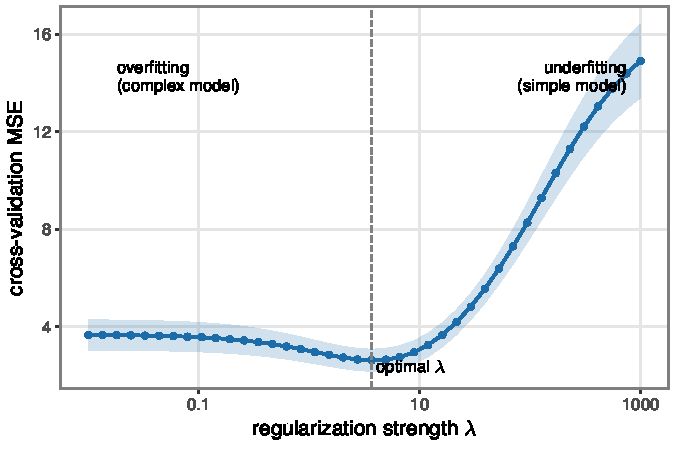
\includegraphics[width=0.6\linewidth]{cv_curve.pdf}
  \caption{Five-fold cross-validation estimate of mean squared error for ridge regression on simulated data ($N=100$, $P=60$), as a function of $\lambda$. The band shows $\pm$ one standard error across folds. Small $\lambda$ overfits and large $\lambda$ underfits.}
  \label{fig:cv_curve}
\end{figure}

\subsection{The bias-variance trade-off}

Let $\vb_0$ denote the true coefficients and $\hat\vb$ an estimate computed from a random training set. For a new input $\vx$, the expected squared error of the prediction $\vx^\top\hat\vb$ for a new response $y=\vx^\top\vb_0+\epsilon$ decomposes as
\begin{equation}
  \E\left[(y-\vx^\top\hat\vb)^2\right] = \underbrace{\left(\E[\vx^\top\hat\vb]-\vx^\top\vb_0\right)^2}_{\text{bias}^2} + \underbrace{\E\left[\left(\vx^\top\hat\vb-\E[\vx^\top\hat\vb]\right)^2\right]}_{\text{variance}} + \underbrace{\sigma^2}_{\text{noise}},
\end{equation}
where the expectations are over training sets and the new noise $\epsilon$. Averaging over new inputs $\vx$ gives the generalization error. The noise term is intrinsic and cannot be reduced. Regularization trades the other two terms against each other (Figure~\ref{fig:bias_var}): increasing $\lambda$ increases bias, because estimates are shrunk away from $\vb_0$, but decreases variance, because estimates depend less on the particular training set. The optimal $\lambda$ minimizes their sum. Section 2.9 of \citet{esl} covers this in more depth.

\begin{figure}[t]
  \centering
  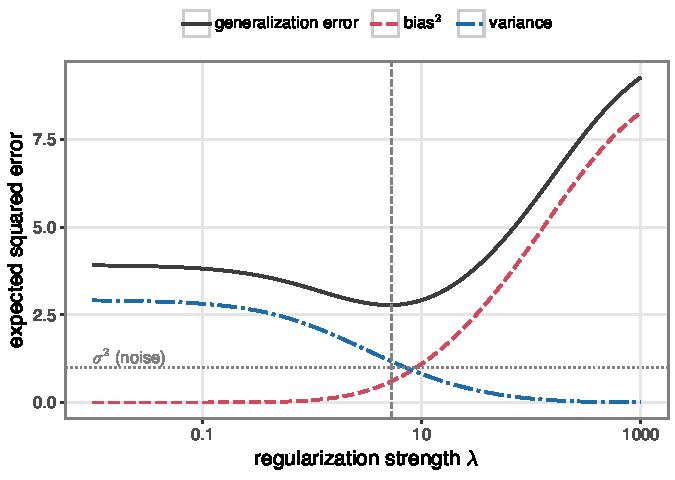
\includegraphics[width=0.6\linewidth]{bias_variance.pdf}
  \caption{Bias-variance decomposition of the expected prediction error of ridge regression for a fixed simulated design ($N=80$, $P=60$, $\sigma^2=1$), computed exactly. Bias increases and variance decreases with $\lambda$; their sum plus the noise variance is the generalization error, minimized at the dashed line.}
  \label{fig:bias_var}
\end{figure}

%======================================================================
\section{L1 regularization and the lasso}
\label{sec:lasso}
%======================================================================

\subsection{A Laplace prior}

Ridge regression follows from a Gaussian prior on each coefficient. If we instead use a Laplace prior with scale $b$, $p(\beta_j)=\frac{1}{2b}\exp(-|\beta_j|/b)$, the log prior contributes $-\frac{1}{b}|\beta_j|$ to the log posterior instead of $-\frac{1}{2\sigma_\beta^2}\beta_j^2$ (Figure~\ref{fig:penalties}). The MAP estimate then minimizes
\begin{equation}
  \frac{1}{2}\sum_{i=1}^N\left(y_i-\vx_i^\top\vb\right)^2 + \lambda\|\vb\|_1, \qquad \|\vb\|_1=\sum_{j=1}^P|\beta_j|,
  \label{eq:lasso}
\end{equation}
with $\lambda=\sigma^2/b$. This is the \emph{lasso}~\citep{tibshirani1996}, or L1-regularized regression. The key property of the lasso is that many coefficients of the solution are exactly zero, which is called \emph{sparsity}. A sparse model uses only a subset of features, which makes it easier to interpret.

\begin{figure}[t]
  \centering
  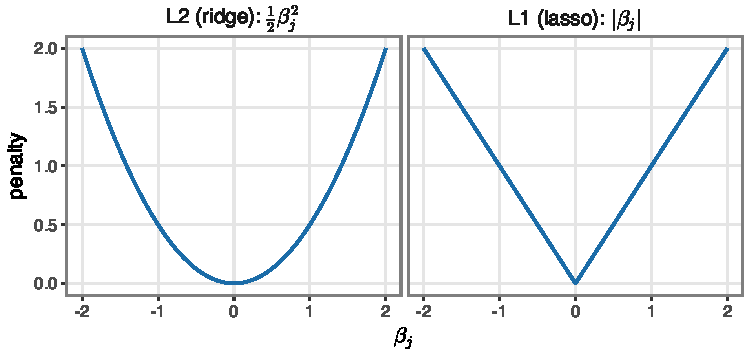
\includegraphics[width=0.75\linewidth]{penalties.pdf}
  \caption{The L2 (ridge) and L1 (lasso) penalties as functions of one coefficient. They are the negative log densities, up to constants, of a Gaussian and a Laplace prior.}
  \label{fig:penalties}
\end{figure}

\subsection{Penalties and constraints}

Each penalized problem is equivalent to a constrained problem: for every $\lambda$ there is a $\gamma$ such that minimizing $\frac{1}{2}\sum_i(y_i-\vx_i^\top\vb)^2+\lambda\|\vb\|$ gives the same solution as minimizing $\sum_i(y_i-\vx_i^\top\vb)^2$ subject to $\|\vb\|\leq\gamma$, where $\|\cdot\|$ is the L2 norm for ridge and the L1 norm for the lasso. The constrained form gives a geometric picture of sparsity (Figure~\ref{fig:constraint}). The contours of the sum of squares are ellipses centred on the OLS estimate. The solution is the first point where an ellipse touches the constraint region. The L2 ball is round, so this point generically has both coordinates non-zero. The L1 ball is a diamond with corners on the axes, and an ellipse is likely to first touch it at a corner, where one coordinate is exactly zero.

At the optimum of the penalized objective $L(\vb)+P(\vb)$, with $L$ the negative log likelihood and $P$ the penalty, the gradient is zero, so $\nabla_{\vb}L=-\nabla_{\vb}P$: the pull of the data toward $\hat\vb_{\text{OLS}}$ is balanced by the pull of the penalty toward zero.

\begin{figure}[t]
  \centering
  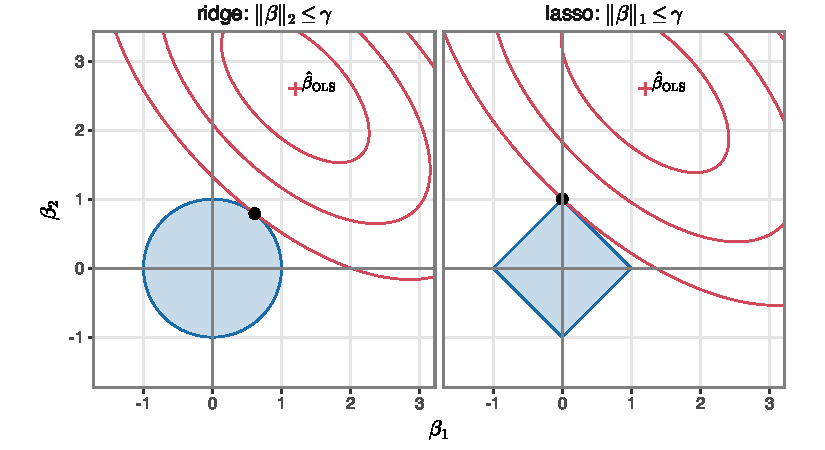
\includegraphics[width=0.85\linewidth]{constraint_geometry.pdf}
  \caption{Least-squares contours (red ellipses, centred on $\hat\vb_{\text{OLS}}$) and constraint regions (shaded) for ridge and lasso. The solution (black point) is where the smallest contour touches the constraint region. The lasso solution lies on a corner of the diamond, so $\beta_1=0$.}
  \label{fig:constraint}
\end{figure}

\subsection{Sparsity in one dimension}

The one-dimensional case shows why the lasso sets coefficients to exactly zero. Consider a single coefficient with an orthonormal design, so that the objective is
\begin{equation}
  f(\beta) = \frac{1}{2}\left(\beta-\hat\beta_{\text{OLS}}\right)^2 + \lambda|\beta| ,
\end{equation}
where $\hat\beta_{\text{OLS}}\in\R$ is the least-squares estimate. The absolute value is not differentiable at zero, so we use its \emph{subgradient} (Section~\ref{sec:convexity}): $\partial|\beta|=\{\operatorname{sign}(\beta)\}$ for $\beta\neq 0$ and $\partial|\beta|=[-1,1]$ at $\beta=0$. The minimizer satisfies $0\in\beta-\hat\beta_{\text{OLS}}+\lambda\,\partial|\beta|$. If $\hat\beta\neq 0$ this gives $\hat\beta=\hat\beta_{\text{OLS}}-\lambda\operatorname{sign}(\hat\beta)$, which is consistent only if $|\hat\beta_{\text{OLS}}|>\lambda$. Otherwise $\hat\beta=0$, which is consistent whenever $|\hat\beta_{\text{OLS}}|\leq\lambda$, since then $\hat\beta_{\text{OLS}}/\lambda\in[-1,1]$. Together,
\begin{equation}
  \hat\beta_{\text{lasso}} = \operatorname{sign}(\hat\beta_{\text{OLS}})\max\left(|\hat\beta_{\text{OLS}}|-\lambda,\,0\right),
\end{equation}
which is called \emph{soft thresholding}. The same argument for ridge gives $\hat\beta_{\text{ridge}}=\hat\beta_{\text{OLS}}/(1+\lambda)$, which shrinks the estimate but never reaches zero. Figure~\ref{fig:objectives} shows the two objectives for several values of $\lambda$, and Figure~\ref{fig:shrinkage} compares the resulting estimates. The intuition is that the gradient of the squared error goes to zero as $\beta$ approaches the OLS estimate, while the gradient of the L1 penalty has constant magnitude $\lambda$. Once $\lambda$ exceeds the gradient of the squared error at zero, the penalty wins and the coefficient stays at zero.

\begin{figure}[t]
  \centering
  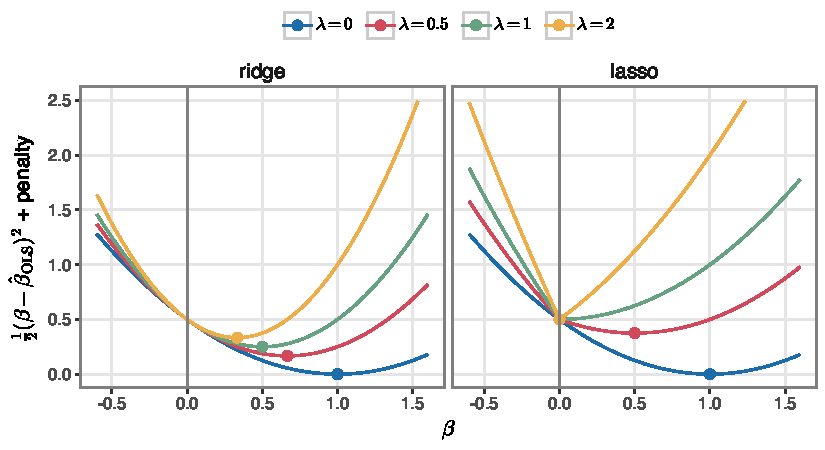
\includegraphics[width=0.85\linewidth]{objectives_1d.pdf}
  \caption{One-dimensional penalized objectives with $\hat\beta_{\text{OLS}}=1$ for several values of $\lambda$; points mark the minimizers. The ridge minimizer moves toward zero but stays positive; the lasso minimizer reaches zero at $\lambda=1$ and stays there.}
  \label{fig:objectives}
\end{figure}

\begin{figure}[t]
  \centering
  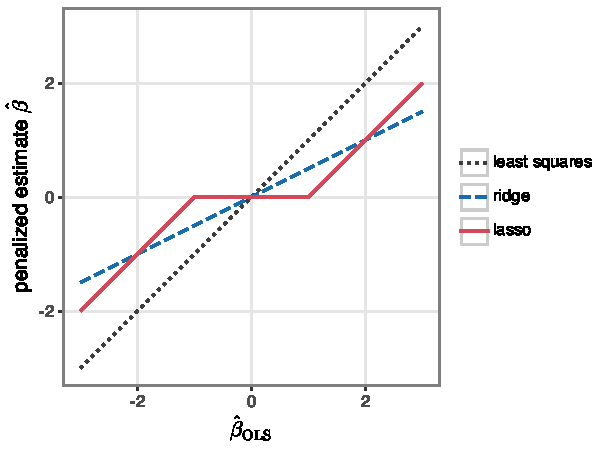
\includegraphics[width=0.5\linewidth]{shrinkage.pdf}
  \caption{Ridge and lasso estimates as functions of the least-squares estimate for an orthonormal design, $\lambda=1$. Ridge scales the estimate by $1/(1+\lambda)$; the lasso subtracts $\lambda$ from its magnitude and sets it to zero when $|\hat\beta_{\text{OLS}}|\leq\lambda$.}
  \label{fig:shrinkage}
\end{figure}

\subsection{Sparse priors}

From the Bayesian viewpoint, L2 regularization corresponds to a Gaussian prior with density proportional to $e^{-\frac{\lambda}{2}\beta^2}$, and L1 regularization to a Laplace prior with density proportional to $e^{-\lambda|\beta|}$. The Laplace density has a sharper peak at zero and heavier tails than the Gaussian (Figure~\ref{fig:sparse_priors}): it favours many coefficients near zero and a few large ones. A more direct encoding of sparsity is the \emph{spike-and-slab} prior~\citep{mitchell1988},
\begin{equation}
  \beta_j \sim \pi\,\Normal(0,\varepsilon^2) + (1-\pi)\,\Normal(0,\sigma^2_{\text{slab}}),
\end{equation}
a mixture of a narrow ``spike'' at zero with variance $\varepsilon^2$ (or a point mass, $\varepsilon\to 0$) and a broad ``slab'' with variance $\sigma^2_{\text{slab}}$, where $\pi\in[0,1]$ is the prior probability that a coefficient is in the spike. Unlike the lasso, the MAP problem under a spike-and-slab prior is not convex, and the posterior is usually explored with Markov chain Monte Carlo or variational methods.

\begin{figure}[t]
  \centering
  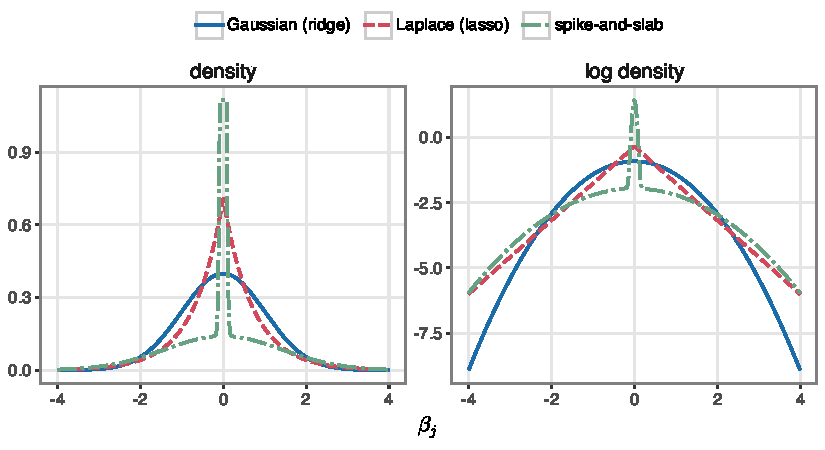
\includegraphics[width=0.85\linewidth]{sparse_priors.pdf}
  \caption{Gaussian, Laplace and spike-and-slab priors with unit variance (spike-and-slab: $\pi=0.5$, $\varepsilon=0.05$, $\sigma^2_{\text{slab}}=2$), on the density (left, truncated) and log density (right) scales. The Gaussian has light tails; the Laplace has a sharp peak at zero and heavier tails.}
  \label{fig:sparse_priors}
\end{figure}

Sections 3.4.2, 3.4.3 and 3.6 of \citet{esl} cover the lasso and its relationship to other variable selection methods.

\subsection{Interpretability}

What makes a machine learning model interpretable? There is no single answer. Properties that are often cited include
\begin{itemize}
  \item linearity, so that each feature's effect is a single number;
  \item sparsity, so that only a few features matter;
  \item causality, so that coefficients describe what would happen under an intervention;
  \item correspondence to a realistic physical, biological or chemical system;
  \item statistical significance or uncertainty estimates for the parameters;
  \item disentangled representations, in which separate latent variables capture separate factors of variation;
  \item being generative, so that the model describes how the data could have arisen.
\end{itemize}
When this question was posed to a class, students emphasized understanding how a model makes its predictions, identifying which variables drive a decision, and being able to explain a model in plain language. They also raised the distinction between interpreting predictions and interpreting features, the possibility that the underlying biological system is not itself simple enough to be interpretable, whether a model yields testable hypotheses about the underlying biology, the trustworthiness of predictions, and, for neural networks, visualizing training dynamics and neuron activations. Sparse linear models score well on several of these criteria, which is one reason they remain popular in genomics.

\subsection{Generalization theory}

Theory makes the benefit of sparsity in high dimensions precise. Let $\vb_0$ be the true coefficients, with $y_i=\vx_i^\top\vb_0+\epsilon_i$. The \emph{out-of-sample risk} (OSR) of an estimate $\hat\vb$ is $\E_{\vx}[(\vx^\top\hat\vb-\vx^\top\vb_0)^2]$, the expected squared difference between estimated and true predictions at a new input. For Gaussian features, the expected OSR of OLS is
\begin{equation}
  \text{OSR}_{\text{OLS}} = \sigma^2\frac{P}{N-P-1},
\end{equation}
which is small only when $P\ll N$ and diverges as $P$ approaches $N$. For the lasso, the risk relative to the best predictor with bounded L1 norm is of order~\citep{greenshtein2004}
\begin{equation}
  \text{OSR}_{\text{lasso}} \sim \|\vb_0\|_1^2\sqrt{\frac{\log P}{N}},
\end{equation}
which grows only logarithmically in the number of features. The lasso can therefore generalize when $\log P$ is small relative to $N$, provided the true coefficients have small L1 norm, as they do when they are sparse. Figure~\ref{fig:risk_vs_p} compares the two expressions. For small $P$ OLS is better, since it is unbiased, but for large $P$ the lasso is far better.

\begin{figure}[t]
  \centering
  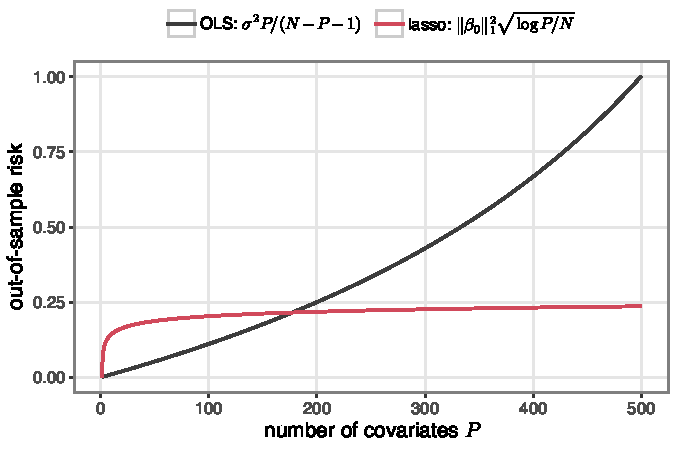
\includegraphics[width=0.6\linewidth]{risk_vs_p.pdf}
  \caption{Out-of-sample risk of OLS and the order of the lasso risk bound as functions of the number of covariates $P$, for $N=1000$, $\sigma^2=1$ and $\|\vb_0\|_1^2=3$. The lasso curve shows the rate only; constants are omitted.}
  \label{fig:risk_vs_p}
\end{figure}

%======================================================================
\section{Optimization}
\label{sec:optimization}
%======================================================================

Ridge regression has a closed-form solution, but the lasso and most models later in this book do not. We then minimize the loss $L(\vb)$ numerically.

\subsection{Gradient descent}

Gradient descent repeatedly takes a step in the direction of steepest descent,
\begin{equation}
  \vb_{\text{new}} = \vb_{\text{current}} - \alpha\nabla_{\vb}L(\vb_{\text{current}}),
\end{equation}
where $\alpha>0$ is the step size (or learning rate) and $\vb$ and $\nabla_{\vb}L$ are both $P$-vectors. Where the loss is steep the steps are large, and as the iterates approach a minimum the gradient, and hence the step, shrinks (Figure~\ref{fig:gd}). For a non-convex loss, gradient descent converges to a local minimum that depends on the starting point.

\begin{figure}[t]
  \centering
  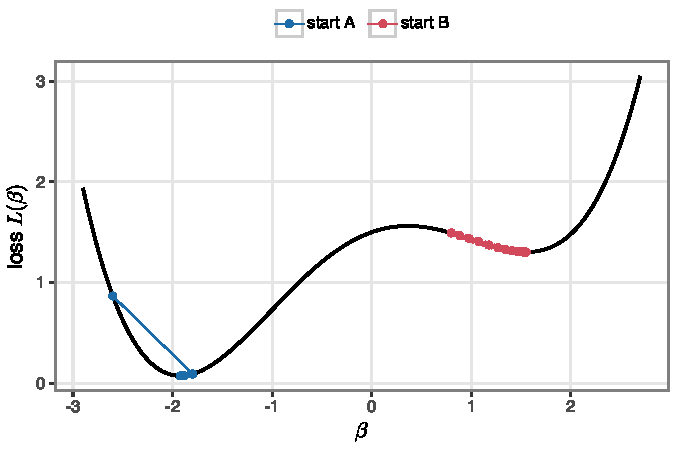
\includegraphics[width=0.6\linewidth]{gradient_descent.pdf}
  \caption{Gradient descent on a non-convex one-dimensional loss from two starting points, with step size $\alpha=0.3$. Each run converges to the local minimum in its basin.}
  \label{fig:gd}
\end{figure}

There are many variants of gradient descent. Common ones are
\begin{itemize}
  \item \emph{momentum} or \emph{acceleration}, which accumulates a running average of past gradients to move faster along consistent directions;
  \item \emph{adaptive step sizes}, either by backtracking line search or with per-parameter scaling as in Adagrad and Adam~\citep{kingma2015};
  \item \emph{minibatch} or \emph{stochastic} gradient descent, which estimates the gradient from a random subset of samples at each step and requires a schedule for decreasing $\alpha$ to converge (adaptive methods such as Adam are often used instead);
  \item \emph{Newton's method}, $\vb_{\text{new}}=\vb_{\text{current}}-(\nabla^2_{\vb}L)^{-1}\nabla_{\vb}L$, which uses the Hessian $\nabla^2_{\vb}L\in\R^{P\times P}$ to rescale the gradient. It converges in few iterations but the Hessian is expensive to compute, store and invert when $P$ is large;
  \item \emph{quasi-Newton methods} such as L-BFGS~\citep{liu1989}, which build a low-rank approximation to the Hessian from successive gradients.
\end{itemize}

\subsection{Convexity and subgradients}
\label{sec:convexity}

A function $f$ is \emph{convex} if, for all $x_1, x_2$ and all $a\in[0,1]$,
\begin{equation}
  f\left(a x_1+(1-a)x_2\right) \leq a f(x_1) + (1-a) f(x_2),
\end{equation}
that is, the chord between any two points on the graph lies on or above the graph (Figure~\ref{fig:convexity}). For a convex function every local minimum is a global minimum, so gradient descent cannot get stuck in a poor local minimum. The least-squares, ridge, lasso and logistic regression losses are all convex. Convex functions can be very flat or very steep, which affects how fast gradient descent converges but not where it converges to.

The absolute value $|\beta|$ is convex but not differentiable at zero. Its gradient is $-1$ for $\beta<0$ and $1$ for $\beta>0$. A \emph{subgradient} of a convex function $f$ at $x$ is any slope $s$ such that the line through $(x, f(x))$ with slope $s$ lies on or below $f$ everywhere. Where $f$ is differentiable the only subgradient is the gradient. At $\beta=0$ every $s\in[-1,1]$ is a subgradient of $|\beta|$. Implementations of subgradient descent often use
\begin{equation}
  \operatorname{sign}(\beta) = \begin{cases} 1, & \beta>0\\ -1, & \beta<0 \\ 0, & \beta=0 \end{cases}
\end{equation}
as the subgradient of $|\beta|$.

\begin{figure}[t]
  \centering
  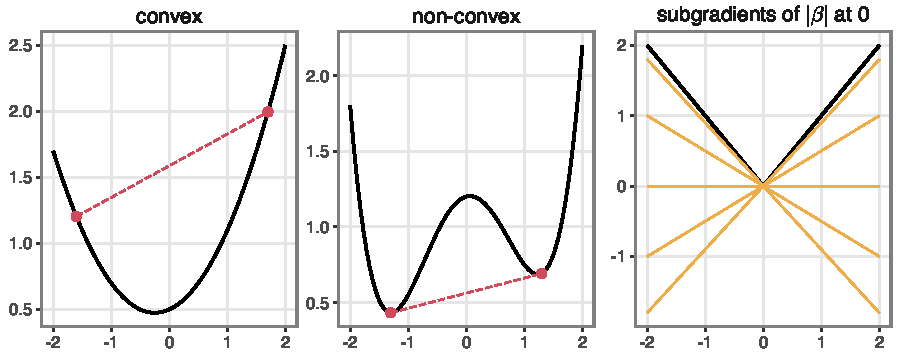
\includegraphics[width=\linewidth]{convexity.pdf}
  \caption{Left: for a convex function the chord between two points lies above the graph. Middle: for a non-convex function some chord passes below the graph. Right: $|\beta|$ is convex but not differentiable at zero, where every line through the origin with slope in $[-1,1]$ (orange) is a subgradient.}
  \label{fig:convexity}
\end{figure}

%======================================================================
\section{Application: elastic net prediction of drug sensitivity}
%======================================================================

\citet{barretina2012} profiled cell lines in CCLE at several molecular levels, including copy number variation (how many copies of each gene are in the genome, which is often altered in cancer), mutation status (single nucleotide variants, insertions and deletions in known oncogenes) and gene expression from microarrays or RNA-seq (Figure~\ref{fig:ccle_data}). To predict drug sensitivity from these features they used the \emph{elastic net}~\citep{zou2005}, which combines the L1 and L2 penalties,
\begin{equation}
  \sum_{i=1}^N\left(y_i-\vx_i^\top\vb\right)^2 + \lambda_1\sum_{j=1}^P|\beta_j| + \frac{\lambda_2}{2}\sum_{j=1}^P\beta_j^2 ,
\end{equation}
with regularization strengths $\lambda_1,\lambda_2\geq0$. The L1 term gives sparsity. The L2 term stabilizes the solution when features are correlated: the lasso tends to select one feature from a correlated group arbitrarily, while the elastic net tends to spread weight across the group.

\begin{figure}[t]
  \centering
  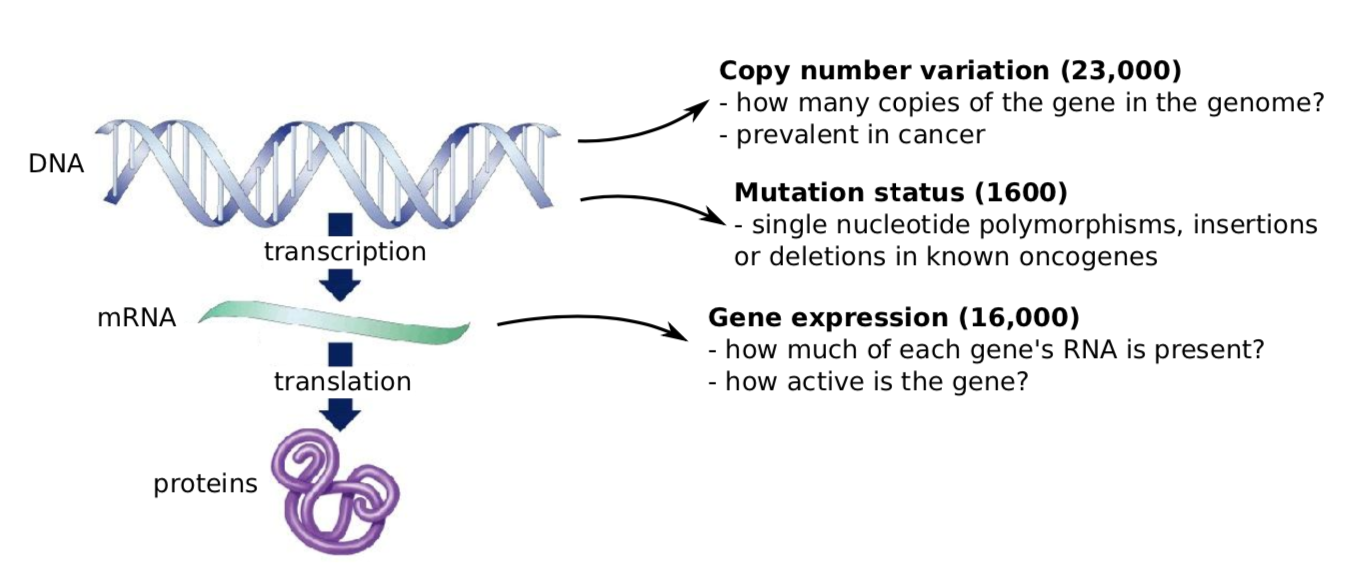
\includegraphics[width=0.8\linewidth]{slides/ccle_data_types.png}
  \caption{Molecular features used to predict drug sensitivity in CCLE: copy number variation and mutation status (from DNA) and gene expression (from mRNA), with the approximate number of genes measured for each. Reproduced from \citet{barretina2012}.}
  \label{fig:ccle_data}
\end{figure}

Figure~\ref{fig:elastic_net} shows the elastic net fit for PD-0325901, an inhibitor of MEK, a kinase in the MAPK signalling pathway. The columns are cell lines sorted by activity area, the response $\vy$, from resistant (left) to sensitive (right). The rows are the selected features, a subset of the columns of $\mX$, shown transposed. The bars on the left are the fitted coefficients $\hat\vb$, and the number after each feature name is how often the feature was selected across bootstrap resamples of the data. Features with large coefficients show visible trends across the heatmap: their values differ between the resistant and the sensitive ends. The selected features include mutations in \textit{NRAS}, \textit{KRAS} and \textit{BRAF}, genes in the MAPK pathway that the drug targets.

\begin{figure}[t]
  \centering
  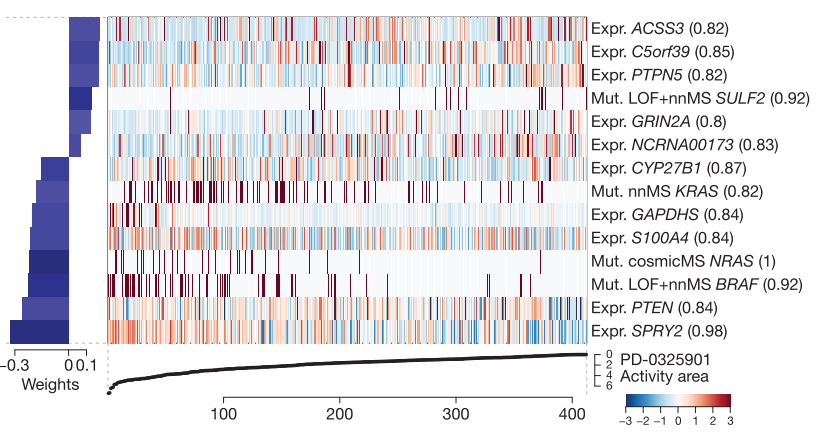
\includegraphics[width=0.9\linewidth]{slides/ccle_elastic_net_pd0325901.png}
  \caption{Elastic net model of sensitivity to the MEK inhibitor PD-0325901. Bottom: activity area $\vy$ for each cell line, sorted from resistant (left) to sensitive (right). Heatmap: standardized values of the selected expression (Expr.) and mutation (Mut.) features in each cell line. Left: fitted coefficients $\hat\vb$. Reproduced from \citet{barretina2012}.}
  \label{fig:elastic_net}
\end{figure}

%======================================================================
\section{Classification and logistic regression}
\label{sec:classification}
%======================================================================

\subsection{Predicting a binary outcome}

Many prediction problems have a binary outcome. Oncotype DX is a gene expression test used to guide treatment of estrogen receptor positive (ER+) breast cancer~\citep{paik2004}. It was developed using tumour expression from approximately 700 patients in an earlier clinical trial of tamoxifen, with the outcome being recurrence or metastasis within 10 years (Figure~\ref{fig:data_matrices}b). Patients predicted to be at high risk are offered chemotherapy, and the test is now part of the standard of care for ER+ breast cancer.

Returning to the cell line example, we might also binarize the response: let $y_i=1$ if cell line $i$ is sensitive to the drug and $y_i=0$ otherwise.

\subsection{Logistic regression}

Logistic regression models the probability that $y_i=1$ as
\begin{equation}
  p(y_i=1\mid\vx_i,\vb) = \sigma(\vx_i^\top\vb) =: p_i, \qquad \sigma(g) = \frac{1}{1+e^{-g}},
  \label{eq:logistic}
\end{equation}
where $\sigma:\R\to(0,1)$ is the logistic sigmoid function (Figure~\ref{fig:sigmoid}) and $p_i\in(0,1)$. An intercept can be included by appending a one to each input, $\vx_i\leftarrow[\vx_i^\top, 1]^\top$. Equivalently,
\begin{equation}
  y_i\mid\vx_i,\vb \sim \text{Bernoulli}(p_i), \qquad p(y_i\mid\vx_i,\vb) = p_i^{y_i}(1-p_i)^{1-y_i},
\end{equation}
independently across samples. The compact form of the Bernoulli probability gives $p_i^1(1-p_i)^0=p_i$ when $y_i=1$ and $p_i^0(1-p_i)^1=1-p_i$ when $y_i=0$. The linear predictor $g_i=\vx_i^\top\vb$ is the log odds, $\log\frac{p_i}{1-p_i}$. The set of inputs with $\vx^\top\vb=0$, where $p=0.5$, is a hyperplane called the \emph{decision boundary}, and lines of constant probability are parallel to it (Figure~\ref{fig:logistic_2d}).

\begin{figure}[t]
  \centering
  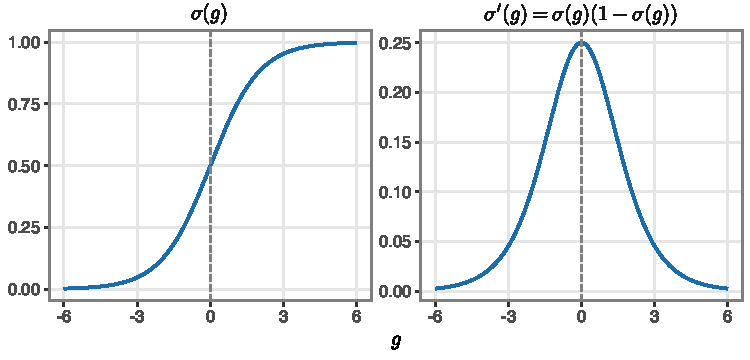
\includegraphics[width=0.75\linewidth]{sigmoid.pdf}
  \caption{The logistic sigmoid $\sigma(g)$ maps the linear predictor to a probability. Its derivative $\sigma'(g)=\sigma(g)(1-\sigma(g))$ is largest at $g=0$.}
  \label{fig:sigmoid}
\end{figure}

\begin{figure}[t]
  \centering
  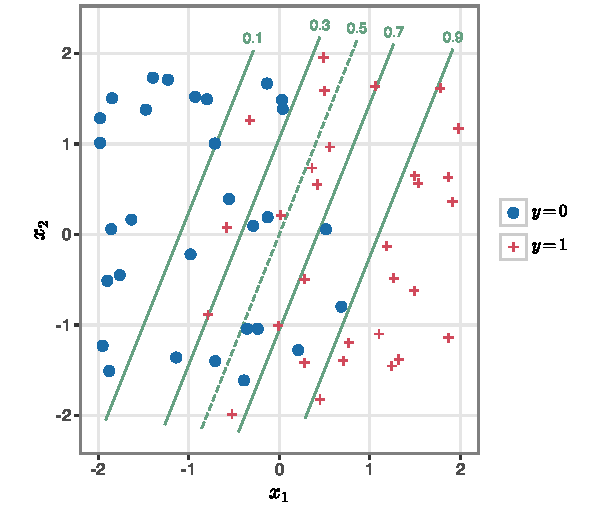
\includegraphics[width=0.55\linewidth]{logistic_2d.pdf}
  \caption{Logistic regression with two features. Lines are contours of the predicted probability $p=\sigma(\vx^\top\vb)$; the dashed line $p=0.5$ is the decision boundary. Points are simulated from the model.}
  \label{fig:logistic_2d}
\end{figure}

As for linear regression, we can place a Gaussian prior on $\vb$ with variance $\sigma_\beta^2$. The model is summarized by the graphical model in Figure~\ref{fig:graphical_model}, where arrows indicate conditional dependence: the prior variance determines the distribution of $\vb$, and $\vb$ together with $\mX$ determines the distribution of $\vy$ through the likelihood.

\begin{figure}[t]
  \centering
  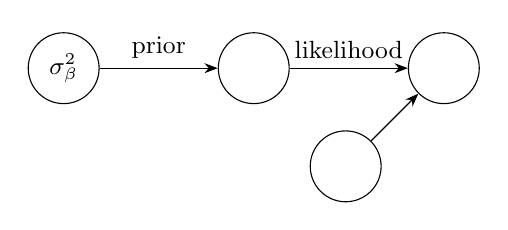
\begin{tikzpicture}[>=Stealth, every node/.style={font=\small}, var/.style={circle, draw, minimum size=0.9cm}]
    \node[var] (s) {$\sigma_\beta^2$};
    \node[var, right=1.5cm of s] (b) {$\vb$};
    \node[var, right=1.5cm of b] (y) {$\vy$};
    \node[var, below left=0.6cm and 0.6cm of y] (x) {$\mX$};
    \draw[->] (s) -- node[above] {prior} (b);
    \draw[->] (b) -- node[above] {likelihood} (y);
    \draw[->] (x) -- (y);
  \end{tikzpicture}
  \caption{Graphical model for (regularized) logistic regression.}
  \label{fig:graphical_model}
\end{figure}

\subsection{Likelihood and the cross-entropy loss}

By independence, the likelihood is
\begin{equation}
  p(\vy\mid\mX,\vb) = \prod_{i=1}^N p(y_i\mid\vx_i,\vb) = \prod_{i=1}^N p_i^{y_i}(1-p_i)^{1-y_i},
\end{equation}
and the log likelihood is
\begin{equation}
  \log p(\vy\mid\mX,\vb) = \sum_{i=1}^N \ell_i, \qquad \ell_i = y_i\log p_i + (1-y_i)\log(1-p_i).
\end{equation}
The loss $-\log p(\vy\mid\mX,\vb)=-\sum_i\ell_i$ is called the \emph{binary cross-entropy}. Unlike linear regression, setting its gradient to zero does not give a closed-form solution, so we minimize it numerically, which requires the gradient $\nabla_{\vb}\sum_i\ell_i=\sum_i\nabla_{\vb}\ell_i$.

\subsection{Calculating the gradient}

The computation of $\ell_i$ from $\vx_i$ and $\vb$ can be written as a chain of simple steps, a \emph{computational graph} (Figure~\ref{fig:compgraph}),
\begin{equation}
  g = \vx_i^\top\vb, \qquad p = \sigma(g), \qquad \ell = y\log p+(1-y)\log(1-p),
\end{equation}
where we drop the subscript $i$ on $g$, $p$, $y$ and $\ell$. Evaluating these steps in order is the \emph{forward pass}. The chain rule states that for a composition $x\to y\to z$, $\frac{\partial z}{\partial x}=\frac{\partial z}{\partial y}\frac{\partial y}{\partial x}$. Applying it to the computational graph, starting from the output, is the \emph{backward pass} or \emph{backpropagation},
\begin{equation}
  \frac{\partial\ell}{\partial\vb} = \frac{\partial\ell}{\partial p}\frac{\partial p}{\partial g}\frac{\partial g}{\partial\vb}.
\end{equation}
The three local derivatives are
\begin{equation}
  \frac{\partial\ell}{\partial p} = \frac{y}{p}-\frac{1-y}{1-p}, \qquad \frac{\partial p}{\partial g} = \sigma(g)\left(1-\sigma(g)\right) = p(1-p), \qquad \frac{\partial g}{\partial\vb} = \vx_i .
\end{equation}
Multiplying the first two, $\frac{\partial\ell}{\partial g} = y(1-p)-(1-y)p = y-p$, so
\begin{equation}
  \nabla_{\vb}\ell_i = (y_i-p_i)\,\vx_i, \qquad \nabla_{\vb}\left(-\sum_{i=1}^N\ell_i\right) = \sum_{i=1}^N(p_i-y_i)\,\vx_i = \mX^\top(\vp-\vy),
  \label{eq:logistic_grad}
\end{equation}
where $\vp\in(0,1)^N$ collects the predicted probabilities. Each sample contributes its feature vector weighted by its prediction error $p_i-y_i$, which mirrors the least-squares gradient $\mX^\top(\mX\vb-\vy)$. Modern software computes such gradients automatically by backpropagation through the computational graph, so we rarely derive them by hand for complex models.

\begin{figure}[t]
  \centering
  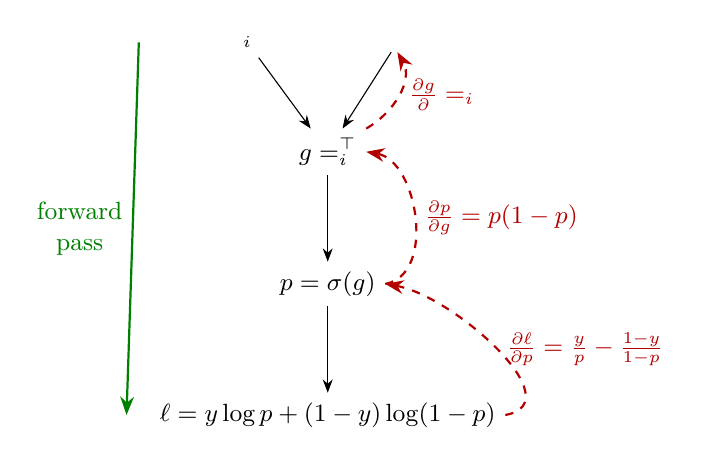
\begin{tikzpicture}[>=Stealth, every node/.style={font=\small}, node distance=1.1cm]
    \node (x) {$\vx_i$};
    \node[right=1.6cm of x] (b) {$\vb$};
    \node[below right=0.9cm and 0.35cm of x] (g) {$g=\vx_i^\top\vb$};
    \node[below=of g] (p) {$p=\sigma(g)$};
    \node[below=of p] (l) {$\ell=y\log p+(1-y)\log(1-p)$};
    \draw[->] (x) -- (g); \draw[->] (b) -- (g);
    \draw[->] (g) -- (p); \draw[->] (p) -- (l);
    \draw[->, green!50!black, thick] ($(x.west)+(-1.2,0)$) -- ($(l.west)+(-0.3,0)$|-l) node[midway, left, align=center] {forward\\pass};
    \draw[->, red!70!black, dashed, thick] (l.east) to[out=10, in=-10] node[right] {$\frac{\partial\ell}{\partial p}=\frac{y}{p}-\frac{1-y}{1-p}$} (p.east);
    \draw[->, red!70!black, dashed, thick] (p.east) to[out=10, in=-10] node[right] {$\frac{\partial p}{\partial g}=p(1-p)$} (g.east);
    \draw[->, red!70!black, dashed, thick] (g.north east) to[out=30, in=-60] node[right] {$\frac{\partial g}{\partial\vb}=\vx_i$} (b.south);
  \end{tikzpicture}
  \caption{Computational graph for the logistic regression log likelihood of one sample. The forward pass (green) computes $\ell$; the backward pass (red) multiplies local derivatives by the chain rule to obtain $\partial\ell/\partial\vb$.}
  \label{fig:compgraph}
\end{figure}

\subsection{Assessing binary classification}
\label{sec:classification_metrics}

Thresholding the predicted probabilities, for example at $0.5$, gives predicted classes. Comparing these to the true classes gives the \emph{confusion matrix} (Table~\ref{tab:confusion}), whose entries are the numbers of true negatives (TN), false negatives (FN), false positives (FP) and true positives (TP). Common summaries are
\begin{gather}
  \text{accuracy} = \frac{\text{TN}+\text{TP}}{\text{TN}+\text{FN}+\text{FP}+\text{TP}}, \qquad
  \text{TPR} = \frac{\text{TP}}{\text{TP}+\text{FN}}, \nonumber\\
  \text{FPR} = \frac{\text{FP}}{\text{FP}+\text{TN}}, \qquad
  \text{precision} = \frac{\text{TP}}{\text{FP}+\text{TP}} ,
\end{gather}
where the true positive rate (TPR) is also called \emph{sensitivity} or \emph{recall}, and the false positive rate (FPR) is one minus the \emph{specificity}.

\begin{table}[t]
  \centering
  \caption{Confusion matrix for binary classification.}
  \label{tab:confusion}
  \begin{tabular}{llcc}
    \toprule
    & & \multicolumn{2}{c}{Truth} \\
    \cmidrule(lr){3-4}
    & & $-$ & $+$ \\
    \midrule
    \multirow{2}{*}{Predicted} & $-$ & TN & FN \\
    & $+$ & FP & TP \\
    \bottomrule
  \end{tabular}
\end{table}

These metrics depend on the threshold. Varying the threshold from high to low traces out the \emph{receiver operating characteristic} (ROC) curve of TPR against FPR, and the \emph{precision-recall} (PR) curve of precision against recall (Figure~\ref{fig:roc_pr}). A random classifier has a diagonal ROC curve and a flat PR curve at the proportion of positives. A better classifier has an ROC curve toward the top left and a PR curve toward the top right. The areas under these curves, AUROC and AUPR, summarize performance across thresholds. AUROC is the probability that a randomly chosen positive is ranked above a randomly chosen negative.

\begin{figure}[t]
  \centering
  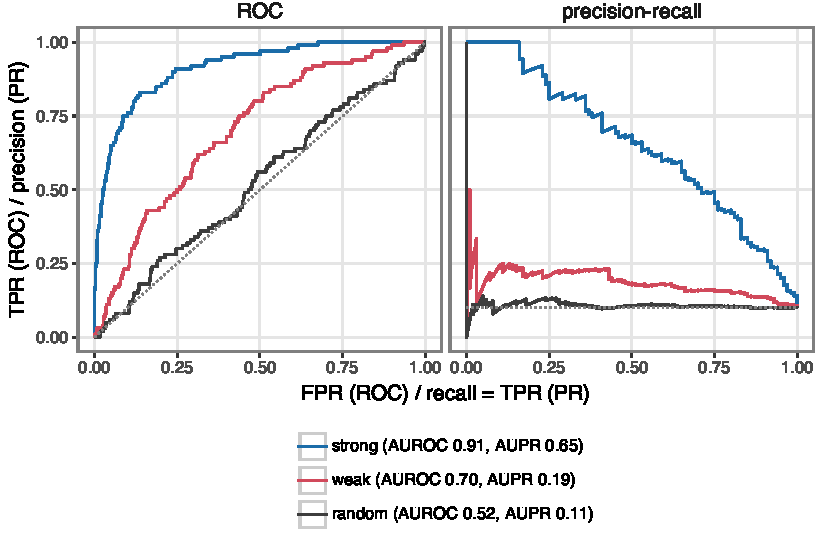
\includegraphics[width=0.85\linewidth]{roc_pr.pdf}
  \caption{ROC (left) and precision-recall (right) curves for simulated classifiers of differing quality, with 10\% positives. Dotted lines show the performance of random guessing. With class imbalance the weak classifier's AUROC of 0.70 looks reasonable, while its AUPR shows that most of its positive predictions are wrong.}
  \label{fig:roc_pr}
\end{figure}

Some practical points:
\begin{itemize}
  \item These metrics should usually be assessed on test data.
  \item AUROC and AUPR depend only on the ranking of predictions, like the Spearman correlation, so they ignore errors such as getting the overall level of the probabilities wrong, which accuracy does not.
  \item With high class imbalance AUROC can look good even when most positive predictions are false; AUPR is then more informative.
  \item The full ROC or PR curve can be valuable, for example in applications where only a very low FPR is acceptable.
  \item Some prediction problems are much harder or noisier than others, so there is no universal threshold for a ``good'' AUROC.
\end{itemize}

%======================================================================
\section{Multiclass classification}
%======================================================================

\subsection{\texorpdfstring{Predicting one of $D$ classes}{Predicting one of D classes}}

Breast cancers can be classified into intrinsic molecular subtypes: luminal A, luminal B, HER2-enriched, basal-like and normal-like. The subtypes were discovered by clustering tumour expression profiles (Figure~\ref{fig:pam50}a) and differ in prognosis (Figure~\ref{fig:pam50}b). PAM50 (Prediction Analysis of Microarray using 50 genes) is a classifier that assigns a tumour to one of these subtypes from the expression of 50 genes, trained on 189 tumour samples from several hospitals~\citep{parker2009}. Predicting one of several classes is a multiclass classification problem.

\begin{figure}[t]
  \centering
  \begin{subfigure}[b]{0.42\linewidth}
    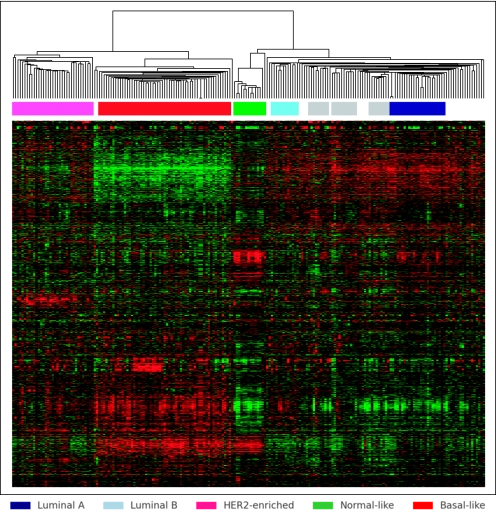
\includegraphics[width=\linewidth]{slides/pam50_heatmap.png}
    \caption{}
  \end{subfigure}\hfill
  \begin{subfigure}[b]{0.52\linewidth}
    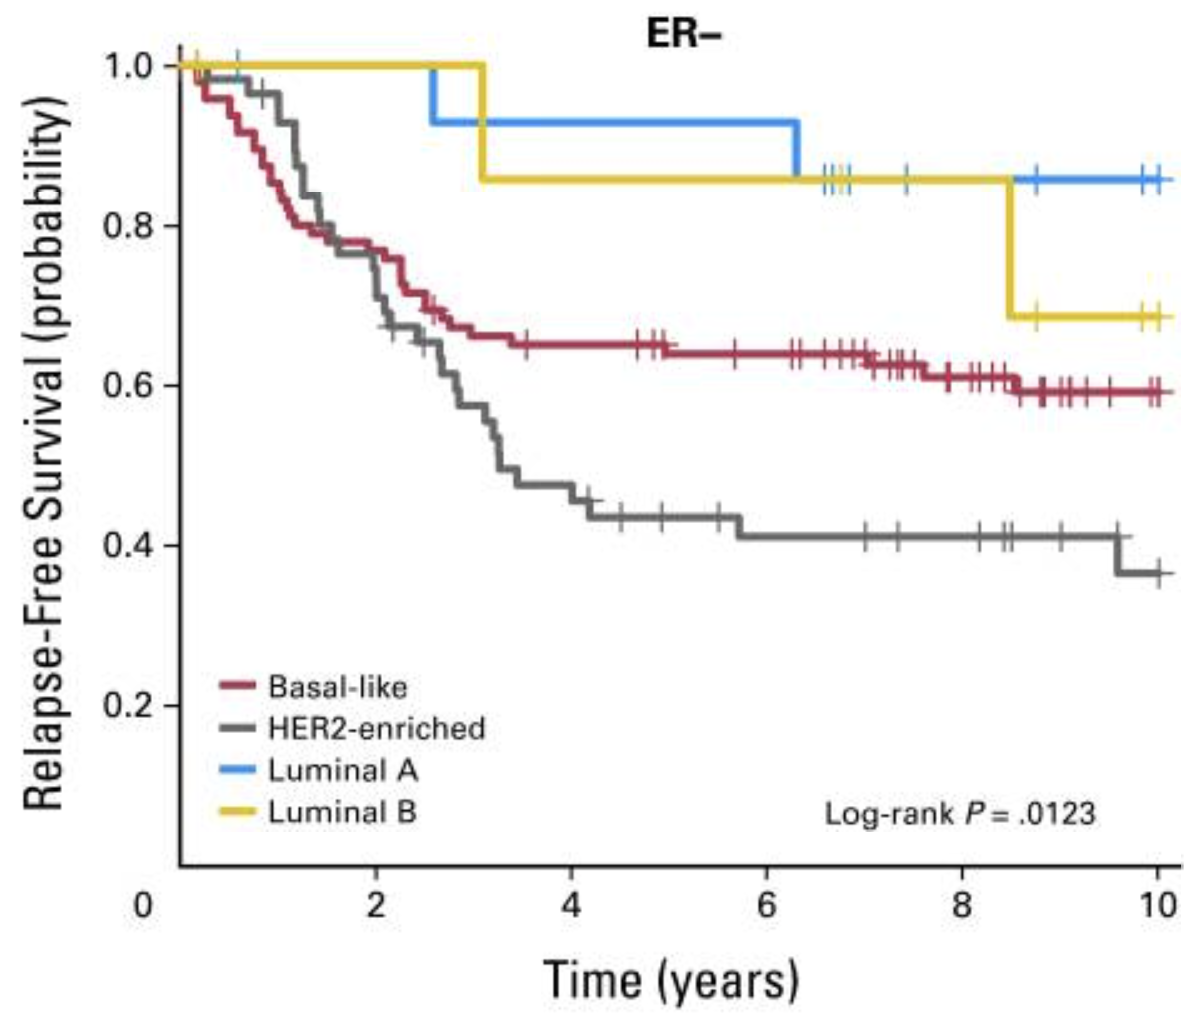
\includegraphics[width=\linewidth]{slides/pam50_survival.png}
    \caption{}
  \end{subfigure}
  \caption{Breast cancer intrinsic subtypes. (a) Hierarchical clustering of tumour gene expression profiles (columns) reveals the subtypes. (b) Relapse-free survival of ER-negative patients differs between subtypes. Reproduced from \citet{parker2009}.}
  \label{fig:pam50}
\end{figure}

\subsection{Multiclass logistic regression}

Let $D$ be the number of classes and $y_i\in\{1,\dots,D\}$ the class of sample $i$. The coefficients now form a matrix $\vb\in\R^{P\times D}$, one column per class, and the linear predictor $\vg_i=\vx_i^\top\vb$ is a $1\times D$ vector with dimensions $[1\times P][P\times D]=[1\times D]$. The \emph{softmax} function maps $\vg_i$ to a vector of probabilities $\vp_i\in\R^D$,
\begin{equation}
  p_{id} = s_d(\vg_i) = \frac{e^{g_{id}}}{\sum_{d'=1}^D e^{g_{id'}}},
\end{equation}
which satisfies $p_{id}\geq 0$ and $\sum_d p_{id}=1$. The model is
\begin{equation}
  y_i\mid\vx_i,\vb \sim \text{Categorical}(\vp_i), \qquad p(y_i\mid\vx_i,\vb) = \prod_{d=1}^D p_{id}^{\ind[y_i=d]},
\end{equation}
where $\ind[\cdot]$ is the indicator function, and the log likelihood of one sample is
\begin{equation}
  \ell_i = \log p(y_i\mid\vx_i,\vb) = \sum_{d=1}^D\ind[y_i=d]\log p_{id}.
\end{equation}
The loss $-\sum_i\ell_i$ is the \emph{cross-entropy loss}. Binary logistic regression is the case $D=2$, with one column of $\vb$ fixed to zero. The gradient follows from the same chain-rule argument as before: $\partial\ell_i/\partial g_{id}=\ind[y_i=d]-p_{id}$, so the gradient of the loss with respect to the $d$-th column of $\vb$ is $\sum_i(p_{id}-\ind[y_i=d])\,\vx_i$.

\subsection{Assessing multiclass classification}

Several metrics extend to the multiclass case.
\begin{itemize}
  \item \emph{Accuracy} (or top-1 accuracy) is how often the most probable class is the true class.
  \item \emph{Top-$k$ accuracy} is how often the true class is among the $k$ most probable classes.
  \item Other metrics, such as AUROC, are computed \emph{one-vs-rest} (OvR): each class in turn is treated as positive and the remaining classes as negative.
\end{itemize}
One-vs-rest metrics must be combined across classes. \emph{Micro averaging} pools the counts (TP, FP, FN) across classes and then computes the metric. It answers how well we do on the average sample, and it is dominated by the most common classes. \emph{Macro averaging} computes the metric for each class and then averages. It answers how well we do on the average class. Standard libraries, for example \texttt{roc\_auc\_score} in scikit-learn with \texttt{multi\_class="ovr"}, provide these options through an \texttt{average} argument.

%======================================================================
\section{Summary}
%======================================================================

\begin{itemize}
  \item The central dogma: DNA is transcribed to RNA, which is translated to protein. Gene expression is the amount of RNA for each gene in a sample, a proxy for protein abundance. RNA-seq measures it by reverse transcribing RNA to DNA, sequencing, aligning reads to the genome and counting reads per gene.
  \item Linear regression predicts a continuous outcome, such as drug sensitivity, from multiple features, such as gene expression. The maximum likelihood estimate under Gaussian noise is the least-squares solution $(\mX^\top\mX)^{-1}\mX^\top\vy$.
  \item Regularization is needed when $P>N$ or features are correlated. A Gaussian prior gives ridge (L2) regression; a Laplace prior gives the lasso (L1), whose solutions are sparse. Hyperparameters are chosen by cross-validation, which balances overfitting and underfitting, or equivalently bias and variance.
  \item Losses without closed-form minimizers are optimized by gradient descent and its variants; convex losses have no spurious local minima.
  \item Logistic regression handles binary outcomes, such as prognosis, and its softmax extension handles multiclass outcomes, such as cancer subtypes. Performance is assessed with metrics such as AUROC and AUPR, preferably on test data.
\end{itemize}

%======================================================================
\section*{Exercises}
%======================================================================

\begin{enumerate}
  \item Derive the MAP estimate~\eqref{eq:ridge} from the log posterior~\eqref{eq:logpost}, and show that the posterior over $\vb$ is Gaussian with covariance $\sigma^2(\mX^\top\mX+\lambda\mI)^{-1}$.
  \item Show that, for the least-squares fit with an intercept, $R^2=1-\text{SS}/\text{TSS}$ equals the squared Pearson correlation between $\vy$ and $\hat\vy$.
  \item Show that for an orthonormal design, $\mX^\top\mX=\mI$, the lasso solution is obtained by soft thresholding each component of $\hat\vb_{\text{OLS}}$.
  \item Compute the Hessian of the binary cross-entropy loss and show that it is positive semi-definite, so the loss is convex.
  \item Implement five-fold cross-validation for ridge regression and apply it to predict the sensitivity of cancer cell lines to one drug from gene expression.
\end{enumerate}

\bibliographystyle{abbrvnat}
\bibliography{../chapter01/chapter01}
\endgroup

% Generated wrapper: chapter 02 with its own figure path, macros and bibliography.
\graphicspath{{../chapter02/figures/}}
\makeatletter\def\input@path{{../chapter02/}}\makeatother
\begingroup
% Chapter 2: deep neural networks, gene regulation and convolutional neural networks.
% Requires: amsmath, amssymb, bm, graphicx, booktabs, multirow, subcaption,
% tikz (arrows.meta, positioning, calc, decorations.pathreplacing, decorations.pathmorphing, shapes.geometric, fit), natbib.
% Computed figures and the tables figures/pwm_example_table.tex and figures/pwm_scan_table.tex are produced by
% scripts/make_figures.py; figures/slides/ holds figures taken from the lecture slides.

\providecommand{\R}{\mathbb{R}}
\providecommand{\E}{\mathbb{E}}
\providecommand{\Normal}{\mathcal{N}}
\providecommand{\argmax}{\operatorname*{arg\,max}}
\providecommand{\argmin}{\operatorname*{arg\,min}}
\providecommand{\vy}{\mathbf{y}}
\providecommand{\vx}{\mathbf{x}}
\providecommand{\mX}{\mathbf{X}}
\providecommand{\mI}{\mathbf{I}}
\providecommand{\vb}{\boldsymbol{\beta}}
\providecommand{\veps}{\boldsymbol{\epsilon}}
\providecommand{\vp}{\mathbf{p}}
\providecommand{\vg}{\mathbf{g}}
\providecommand{\ind}{\mathbf{1}}
\providecommand{\mB}{\mathbf{B}}
\providecommand{\mA}{\mathbf{A}}
\providecommand{\mW}{\mathbf{W}}
\providecommand{\mP}{\mathbf{P}}
\providecommand{\mY}{\mathbf{Y}}
\providecommand{\mZ}{\mathbf{Z}}
\providecommand{\vh}{\mathbf{h}}
\providecommand{\vo}{\mathbf{o}}
\providecommand{\vu}{\mathbf{u}}
\providecommand{\vc}{\mathbf{c}}
\providecommand{\vm}{\mathbf{m}}
\providecommand{\vv}{\mathbf{v}}
\providecommand{\va}{\boldsymbol{\alpha}}
\providecommand{\vtheta}{\boldsymbol{\theta}}
\providecommand{\vdelta}{\boldsymbol{\delta}}
\providecommand{\Loss}{\mathcal{L}}
\providecommand{\vgamma}{\boldsymbol{\gamma}}

\chapter{Deep neural networks and gene regulation}
\label{ch:cnn}

Chapter 1 developed linear models for predicting a response, such as drug sensitivity, from features, such as gene expression. This chapter has three parts. The first extends those models to deep neural networks, which can represent nonlinear functions and interactions between features, and describes how they are fit: backpropagation to compute gradients and stochastic gradient descent to use them. The second part returns to biology and asks \emph{how} cells control which genes are expressed. A central mechanism is the binding of transcription factors to short DNA sequence patterns called motifs, which can be measured genome-wide with ChIP-seq. The third part brings the two together. The classical model of transcription factor binding, the position weight matrix, turns out to be a single convolutional filter, and stacking such filters with nonlinearities and pooling gives a convolutional neural network (CNN) that predicts binding from DNA sequence.

%======================================================================
\section{Beyond linear models}
\label{sec:beyond_linear}
%======================================================================

Linear models have two limitations that matter in practice (Figure~\ref{fig:limitations}). The first is \emph{nonlinearity}. If the response depends on a feature through a curve, a straight line fits poorly however much data we have. The second, less obvious, limitation is the absence of \emph{interaction effects}. An interaction is present when the effect of one feature on the response depends on the value of another. In the classification example of Figure~\ref{fig:limitations}b the positive samples occupy a bounded region of the $(x_1,x_2)$ plane, and no single line separates them from the negatives.

A classical fix is to add interaction terms to a linear model. With two features,
\begin{equation}
  y_i = \beta_1 x_{i1} + \beta_2 x_{i2} + \beta_{12}x_{i1}x_{i2} + \epsilon_i ,
\end{equation}
where $\beta_{12}\in\R$ is the interaction coefficient, or, for classification, $p(y_i=1\mid\vx_i)=\sigma(\beta_1x_{i1}+\beta_2x_{i2}+\beta_{12}x_{i1}x_{i2})$ with $\sigma$ the logistic function of Chapter 1. Polynomial terms such as $x_{i1}^2$ can similarly capture curvature. This works for a handful of features but does not scale. With $P$ features there are $P(P-1)/2$ pairwise interactions; for $P=20{,}000$ genes that is about $2\times10^8$ coefficients, before considering three-way interactions or curvature. We need models that learn which nonlinear combinations of features matter, rather than enumerating them.

\begin{figure}[t]
  \centering
  \begin{subfigure}[b]{0.48\linewidth}
    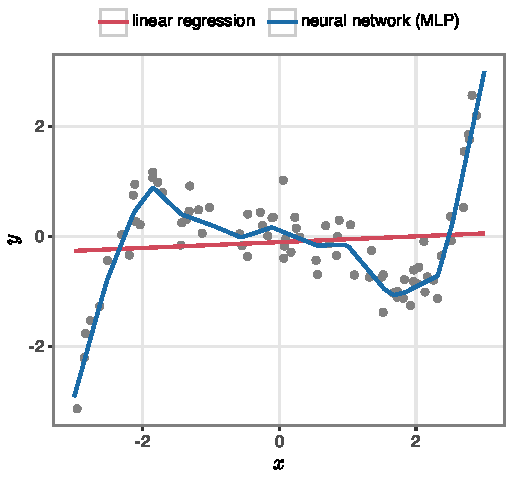
\includegraphics[width=\linewidth]{limitations_nonlinear.pdf}
    \caption{}
  \end{subfigure}\hfill
  \begin{subfigure}[b]{0.48\linewidth}
    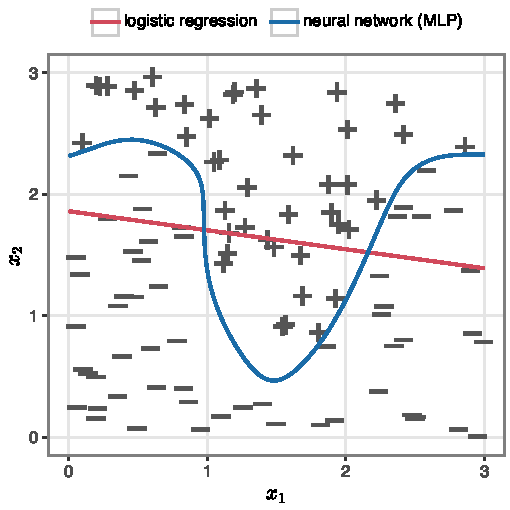
\includegraphics[width=\linewidth]{limitations_interaction.pdf}
    \caption{}
  \end{subfigure}
  \caption{Two limitations of linear models, on simulated data. (a) Nonlinearity: the least-squares line misses the curved relationship between $x$ and $y$, which a small neural network captures. (b) Interaction: positives ($+$) lie inside a disc and negatives ($-$) outside. The logistic regression decision boundary ($p=0.5$) is a line and cannot enclose the positives; a neural network classifier's boundary can.}
  \label{fig:limitations}
\end{figure}

Many nonlinear methods exist. Kernel methods, including support vector machines and Gaussian processes, implicitly map the features into a high-dimensional space in which a linear model is fit. Decision trees partition the feature space by a sequence of thresholds on single features, and ensembles of trees (random forests and gradient boosting) are among the most accurate methods for tabular data. We focus on neural networks because they are the basis of most current models of genomic sequence, and because they are fit with the same gradient-based machinery as the linear models of Chapter 1.

%======================================================================
\section{Neural networks}
\label{sec:mlp}
%======================================================================

\subsection{From logistic regression to a hidden layer}

Recall logistic regression for sample $i$ with features $\vx_i\in\R^P$: the linear predictor $g_i=\vx_i^\top\vb$ is passed through the logistic sigmoid to give a probability. A neural network keeps this building block but uses many copies of it. Let $H$ be the number of \emph{hidden units} (or neurons). Hidden unit $k\in\{1,\dots,H\}$ has its own coefficient vector $\vb_k\in\R^P$ and computes
\begin{equation}
  h_{ik} = \sigma\big(\underbrace{\vx_i^\top}_{1\times P}\underbrace{\vb_k}_{P\times1}\big),
\end{equation}
where $\sigma:\R\to\R$ is a fixed nonlinear \emph{activation function}. Stacking the columns $\vb_1,\dots,\vb_H$ into a weight matrix $\mB\in\R^{P\times H}$, the whole \emph{hidden layer} is
\begin{equation}
  \underbrace{\vh_i^\top}_{1\times H} = \sigma\big(\underbrace{\vx_i^\top}_{1\times P}\underbrace{\mB}_{P\times H}\big),
  \label{eq:hidden}
\end{equation}
with $\sigma$ applied elementwise. The \emph{output layer} is a linear function of the hidden units. With $D$ outputs and a second weight matrix $\mA\in\R^{H\times D}$ whose $d$-th column is $\va_d\in\R^H$,
\begin{equation}
  o_{id} = \vh_i^\top\va_d, \qquad \underbrace{\vo_i^\top}_{1\times D} = \underbrace{\vh_i^\top}_{1\times H}\underbrace{\mA}_{H\times D}.
  \label{eq:output}
\end{equation}
Intercepts (called \emph{biases} in the neural network literature) are included by appending a constant 1 to $\vx_i$ and to $\vh_i$, as in Chapter 1; we leave them implicit. The network is drawn as a graph in Figure~\ref{fig:mlp}, with one node per input, hidden unit and output, and one edge per weight: the edge from $x_{ip}$ to $h_{ik}$ carries $B_{pk}$.

The outputs $\vo_i\in\R^D$ are used exactly as the linear predictor was in Chapter 1. For regression, $\vo_i$ is the prediction of a continuous response and the loss is the squared error. For binary classification, $D=1$ and $\sigma(o_i)$ is the probability that $y_i=1$, with the binary cross-entropy loss. For multiclass classification, $D$ is the number of classes, the softmax of $\vo_i$ gives a probability vector, and the loss is the cross-entropy. Logistic regression is the special case with no hidden layer.

\begin{figure}[t]
  \centering
  \begin{tikzpicture}[>=Stealth, every node/.style={font=\small},
      unit/.style={circle, draw, minimum size=0.8cm, inner sep=0pt}]
    \foreach \j/\lab in {1/$x_{i1}$, 2/$x_{i2}$, 3/$x_{i3}$}
      \node[unit, draw=red!70!black] (x\j) at ({1.6*\j+0.8}, 0) {\lab};
    \foreach \k/\lab in {1/$h_{i1}$, 2/$h_{i2}$, 3/$h_{i3}$, 4/$h_{i4}$}
      \node[unit, draw=blue!70!black] (h\k) at ({1.6*\k}, -1.8) {\lab};
    \foreach \d/\lab in {1/$o_{i1}$, 2/$o_{i2}$}
      \node[unit, draw=green!50!black] (o\d) at ({1.6*\d+1.6}, -3.6) {\lab};
    \foreach \j in {1,2,3} \foreach \k in {1,2,3,4} \draw[->, gray] (x\j) -- (h\k);
    \foreach \k in {1,2,3,4} \foreach \d in {1,2} \draw[->, gray] (h\k) -- (o\d);
    \draw[->, thick] (x1) -- node[left, pos=0.45] {$B_{12}$} (h2);
    \node[right, align=left] at (7.3,0) {input, $\vx_i\in\R^P$};
    \node[right, align=left] at (7.3,-1.8) {hidden, $\vh_i^\top=\sigma(\vx_i^\top\mB)$, $\mB\in\R^{P\times H}$};
    \node[right, align=left] at (7.3,-3.6) {output, $\vo_i^\top=\vh_i^\top\mA$, $\mA\in\R^{H\times D}$};
  \end{tikzpicture}
  \caption{A neural network with one hidden layer, here with $P=3$ inputs, $H=4$ hidden units and $D=2$ outputs. Each edge carries one weight; the highlighted edge from $x_{i1}$ to $h_{i2}$ carries $B_{12}$.}
  \label{fig:mlp}
\end{figure}

\subsection{Activation functions}

Early neural networks used the logistic sigmoid as the activation function. Most current networks use the \emph{rectified linear unit} (ReLU)~\citep{nair2010},
\begin{equation}
  \operatorname{ReLU}(z) = \max(z,0),
\end{equation}
which is zero for negative inputs and the identity for positive inputs. Smooth variants such as the Gaussian error linear unit, $\operatorname{GELU}(z)=z\,\Phi(z)$ with $\Phi$ the standard normal cumulative distribution function~\citep{hendrycks2016}, are common in large models (Figure~\ref{fig:activations}). The ReLU's gradient is 1 for any positive input, whereas the sigmoid's gradient $\sigma(z)(1-\sigma(z))$ vanishes for large $|z|$, which slows gradient-based training of deep networks.

The nonlinearity is essential. Without it, $\vo_i^\top=\vx_i^\top\mB\mA$, which is a linear model with coefficient matrix $\mB\mA\in\R^{P\times D}$. Adding layers to a linear network adds parameters but not expressive power.

\begin{figure}[t]
  \centering
  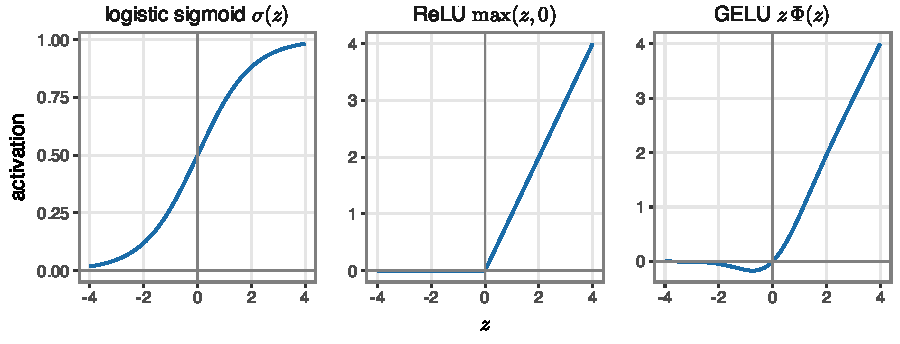
\includegraphics[width=\linewidth]{activations.pdf}
  \caption{Common activation functions. $\Phi$ is the standard normal cumulative distribution function.}
  \label{fig:activations}
\end{figure}

\subsection{Deep networks}

Hidden layers can be stacked. Let $\vh_i^{(0)}=\vx_i$ and $H_0=P$. A network with $M$ hidden layers of widths $H_1,\dots,H_M$ computes
\begin{equation}
  \vh_i^{(m)\top} = \sigma\big(\vh_i^{(m-1)\top}\mB^{(m)}\big), \quad m=1,\dots,M, \qquad \vo_i^\top = \vh_i^{(M)\top}\mA,
\end{equation}
with weight matrices $\mB^{(m)}\in\R^{H_{m-1}\times H_m}$ and $\mA\in\R^{H_M\times D}$. This architecture, in which every unit in one layer connects to every unit in the next, is called a \emph{fully connected} or \emph{dense} network, or a \emph{multilayer perceptron} (MLP), a name that dates from early models of neurons. ``Deep'' refers to having more than one hidden layer.

What functions does an MLP represent? With ReLU activations each hidden unit is a linear function of its inputs followed by a hinge, so the network computes a continuous, piecewise linear function of $\vx_i$. Each layer can bend the function in new places, so deeper networks divide the input space into more linear pieces. Figure~\ref{fig:mlp_random} shows functions of a one-dimensional input computed by small MLPs with random weights: with one hidden layer of five units there are at most five kinks, while with four hidden layers the function is considerably more complex. A one-hidden-layer network can approximate any continuous function on a bounded domain arbitrarily well if $H$ is large enough~\citep{hornik1989}, but deeper networks can represent many functions with far fewer units.

\begin{figure}[t]
  \centering
  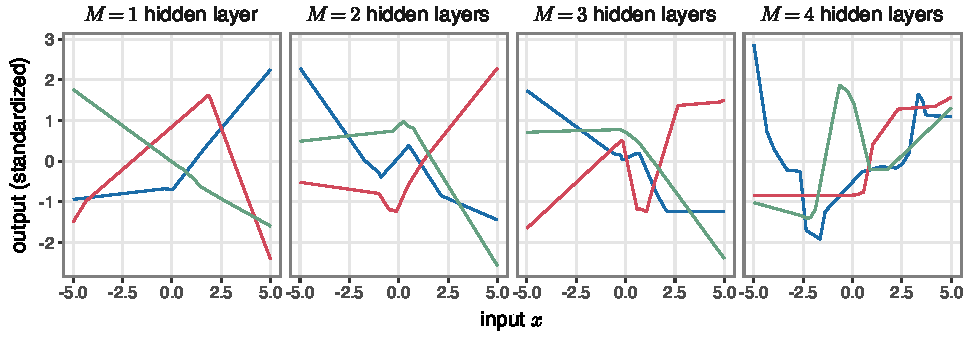
\includegraphics[width=\linewidth]{mlp_random.pdf}
  \caption{Functions computed by ReLU MLPs with one input, $M$ hidden layers of five units and one output, with weights and biases drawn from $\Normal(0,1)$. Each colour is a different random network; outputs are standardized for display. The functions are continuous and piecewise linear, with more pieces as depth increases.}
  \label{fig:mlp_random}
\end{figure}

A network with thousands or millions of parameters can fit its training data perfectly, so overfitting is a real risk. Deep learning practice combines very flexible models with regularization: L2 penalties on the weights (called weight decay), early stopping based on validation loss, dropout, data augmentation and others. Even so, large networks often generalize better than classical theory based on parameter counts would predict~\citep{zhang2017}. One explanation is that gradient-based training tends to find minima of the loss that occupy a large volume of parameter space (``flat'' minima), and these tend to generalize well~\citep{hochreiter1997}. Why this works so well is still an active research question. In practice, repeated training runs from different random initializations usually reach similar performance, although the fitted weights differ.

%======================================================================
\section{Backpropagation}
\label{sec:backprop}
%======================================================================

To fit a neural network by gradient descent we need the gradient of the loss with respect to every weight. Chapter 1 computed the logistic regression gradient by the chain rule along a computational graph. Neural networks are deeper graphs, and the same idea, applied systematically, is \emph{backpropagation}~\citep{rumelhart1986}.

\subsection{The multivariate chain rule}

For scalars, if $y$ depends on $x$ through $u$, $x\to u\to y$, then $\frac{\partial y}{\partial x}=\frac{\partial y}{\partial u}\frac{\partial u}{\partial x}$. Now let $\vx\in\R^{I}$, $\vu\in\R^{J}$ and $\vy\in\R^{K}$, with $\vu$ a function of $\vx$ and $\vy$ a function of $\vu$. A change in $x_i$ affects $y_k$ through every $u_j$, and the contributions add,
\begin{equation}
  \frac{\partial y_k}{\partial x_i} = \sum_{j=1}^{J}\frac{\partial u_j}{\partial x_i}\frac{\partial y_k}{\partial u_j}.
\end{equation}
Define the gradient matrix $\nabla_{\vx}\vy\in\R^{I\times K}$ by $(\nabla_{\vx}\vy)_{ik}=\partial y_k/\partial x_i$, with one row per input and one column per output, and similarly $\nabla_{\vx}\vu\in\R^{I\times J}$ and $\nabla_{\vu}\vy\in\R^{J\times K}$. The sum is then a matrix product, $(\mathbf{A}\mathbf{C})_{ik}=\sum_j A_{ij}C_{jk}$, so
\begin{equation}
  \underbrace{\nabla_{\vx}\vy}_{I\times K} = \underbrace{(\nabla_{\vx}\vu)}_{I\times J}\,\underbrace{(\nabla_{\vu}\vy)}_{J\times K}.
\end{equation}
For a scalar loss $\ell$, $\nabla_{\vx}\ell\in\R^{I}$ is the usual gradient vector, consistent with Chapter 1. For a longer chain $\vx\to\vu^{(1)}\to\cdots\to\vu^{(M)}\to\ell$, the gradient is a product of $M+1$ matrices. Multiplying from the right, starting at the loss, means every intermediate product is a vector rather than a matrix, which is much cheaper. That is the order backpropagation uses.

\subsection{Gradients of a one-hidden-layer network}

Consider one sample with input $\vx\in\R^P$ and continuous targets $\vy\in\R^D$, a network with sigmoid hidden units, and the squared-error loss. We drop the sample index $i$. The forward pass computes, in order,
\begin{equation}
  \underbrace{\vg^\top}_{1\times H} = \vx^\top\mB, \qquad \vh = \sigma(\vg), \qquad \underbrace{\vo^\top}_{1\times D} = \vh^\top\mA, \qquad \ell = \frac12\sum_{d=1}^D(o_d-y_d)^2,
\end{equation}
where $g_k=\sum_p x_pB_{pk}$ and $o_d=\sum_k h_kA_{kd}$ (Figure~\ref{fig:backprop}). The backward pass applies the chain rule from the loss downward, reusing each derivative once it has been computed.
\begin{enumerate}
  \item Output: $\dfrac{\partial\ell}{\partial o_d} = o_d - y_d$. Write $\vdelta_{o}=\vo-\vy\in\R^D$.
  \item Output weights: $A_{kd}$ affects $\ell$ only through $o_d$, and $\partial o_d/\partial A_{kd}=h_k$, so
  \begin{equation}
    \frac{\partial\ell}{\partial A_{kd}} = \frac{\partial\ell}{\partial o_d}\frac{\partial o_d}{\partial A_{kd}} = (o_d-y_d)\,h_k, \qquad \underbrace{\nabla_{\mA}\ell}_{H\times D} = \underbrace{\vh}_{H\times1}\underbrace{\vdelta_o^\top}_{1\times D}.
  \end{equation}
  \item Hidden units: $h_k$ affects every output, with $\partial o_d/\partial h_k=A_{kd}$, so
  \begin{equation}
    \frac{\partial\ell}{\partial h_k} = \sum_{d=1}^D\frac{\partial\ell}{\partial o_d}\frac{\partial o_d}{\partial h_k} = \sum_{d=1}^D(o_d-y_d)A_{kd}, \qquad \vdelta_h = \mA\vdelta_o\in\R^H.
  \end{equation}
  \item Pre-activations: $h_k=\sigma(g_k)$ and $\sigma'(g)=\sigma(g)(1-\sigma(g))$, so
  \begin{equation}
    \frac{\partial\ell}{\partial g_k} = \frac{\partial\ell}{\partial h_k}\,\sigma'(g_k) = \frac{\partial\ell}{\partial h_k}\,h_k(1-h_k), \qquad \vdelta_g = \vdelta_h\odot\vh\odot(\mathbf{1}-\vh),
  \end{equation}
  where $\odot$ is the elementwise product.
  \item First-layer weights: $B_{pk}$ affects $\ell$ only through $g_k$, and $\partial g_k/\partial B_{pk}=x_p$, so
  \begin{equation}
    \frac{\partial\ell}{\partial B_{pk}} = \frac{\partial\ell}{\partial g_k}\,x_p, \qquad \underbrace{\nabla_{\mB}\ell}_{P\times H} = \underbrace{\vx}_{P\times1}\underbrace{\vdelta_g^\top}_{1\times H}.
  \end{equation}
\end{enumerate}
The pattern generalizes to any depth. The gradient with respect to a weight matrix is the outer product of the layer's input and the ``error signal'' $\vdelta$ arriving from above, and the error signal is passed down a layer by multiplying by the transposed weights and the derivative of the activation. With a ReLU activation, step 4 becomes $\delta_{g,k}=\delta_{h,k}\ind[g_k>0]$. The cost of the backward pass is about the same as that of the forward pass. Libraries such as PyTorch, TensorFlow and JAX build the computational graph during the forward pass and compute these gradients automatically (\emph{automatic differentiation}), so in practice we write only the forward pass.

\begin{figure}[t]
  \centering
  \begin{tikzpicture}[>=Stealth, every node/.style={font=\small}, node distance=0.9cm]
    \node (x) {$\vx\ [P]$};
    \node[right=1.4cm of x] (B) {$\mB\ [P\times H]$};
    \node[below=of $(x)!0.5!(B)$] (g) {$\vg^\top=\vx^\top\mB\ [1\times H]$};
    \node[below=of g] (h) {$\vh=\sigma(\vg)\ [H]$};
    \node[right=1.6cm of h] (A) {$\mA\ [H\times D]$};
    \node[below=of $(h)!0.5!(A)$] (o) {$\vo^\top=\vh^\top\mA\ [1\times D]$};
    \node[below=of o] (l) {$\ell=\frac12\sum_d(o_d-y_d)^2$};
    \draw[->] (x) -- (g); \draw[->] (B) -- (g); \draw[->] (g) -- (h);
    \draw[->] (h) -- (o); \draw[->] (A) -- (o); \draw[->] (o) -- (l);
    \begin{scope}[red!70!black, every node/.style={font=\footnotesize, red!70!black}]
      \node[right=0.3cm of l, align=left] {$\partial\ell/\partial o_d=o_d-y_d$};
      \node[right=0.2cm of o.east, align=left] {$\partial\ell/\partial A_{kd}=(o_d-y_d)h_k$};
      \node[left=0.2cm of h.west, align=right] {$\partial\ell/\partial h_k=\sum_d(o_d-y_d)A_{kd}$};
      \node[left=0.2cm of g.west, align=right] {$\partial\ell/\partial g_k=\frac{\partial\ell}{\partial h_k}\sigma'(g_k)$\\$\partial\ell/\partial B_{pk}=\frac{\partial\ell}{\partial g_k}x_p$};
    \end{scope}
  \end{tikzpicture}
  \caption{Computational graph of a one-hidden-layer network with squared-error loss, with the dimension of each quantity in brackets. The forward pass runs top to bottom; the backward pass (red) computes the derivatives from the bottom up, each from the one below it.}
  \label{fig:backprop}
\end{figure}

%======================================================================
\section{Stochastic gradient descent}
\label{sec:sgd}
%======================================================================

\subsection{Minibatch gradients}

Let $\vtheta$ collect all the weights of the network. The loss over a training set of $N$ samples is usually written as an average,
\begin{equation}
  \Loss(\vtheta) = \frac1N\sum_{i=1}^N\ell_i(\vtheta), \qquad \ell_i(\vtheta)=\ell(\vx_i,\vy_i,\vtheta),
\end{equation}
where $\ell$ is the per-sample loss (squared error, binary cross-entropy or cross-entropy). Averaging rather than summing makes the scale of the loss, and so a good step size, independent of $N$. Gradient descent (Chapter 1) needs $\nabla_{\vtheta}\Loss$, which costs a pass over all $N$ samples per step. Genomic data sets for neural networks often have millions of training sequences, so this is slow.

\emph{Stochastic gradient descent} (SGD) replaces the full gradient by an estimate from a random subset of samples, a \emph{minibatch} $\mathcal{B}\subset\{1,\dots,N\}$ of size $|\mathcal{B}|$,
\begin{equation}
  \nabla_{\vtheta}\Loss_{\mathcal{B}} = \frac{1}{|\mathcal{B}|}\sum_{i\in\mathcal{B}}\nabla_{\vtheta}\ell_i .
\end{equation}
If $\mathcal{B}$ is drawn uniformly at random, each sample $i$ is included with probability $|\mathcal{B}|/N$, so
\begin{equation}
  \E_{\mathcal{B}}\left[\nabla_{\vtheta}\Loss_{\mathcal{B}}\right] = \frac{1}{|\mathcal{B}|}\sum_{i=1}^N\Pr(i\in\mathcal{B})\,\nabla_{\vtheta}\ell_i = \frac{1}{|\mathcal{B}|}\frac{|\mathcal{B}|}{N}\sum_{i=1}^N\nabla_{\vtheta}\ell_i = \nabla_{\vtheta}\Loss .
\end{equation}
The minibatch gradient is an unbiased estimate of the full gradient. The update at iteration $t$ is
\begin{equation}
  \vtheta_{t+1} = \vtheta_t - \alpha_t\nabla_{\vtheta}\Loss_{\mathcal{B}_t}(\vtheta_t),
\end{equation}
with a fresh minibatch $\mathcal{B}_t$ at every step. In practice the training set is shuffled and split into consecutive minibatches; one pass through all of them is an \emph{epoch}.

Because the gradient is noisy, a fixed step size makes the iterates keep bouncing around the minimum. Convergence requires a decreasing step size, with $\sum_t\alpha_t=\infty$ (so the iterates can travel any distance) and $\sum_t\alpha_t^2<\infty$ (so the accumulated noise is finite)~\citep{robbins1951}. The schedule $\alpha_t=c/t$ for a constant $c>0$ satisfies both. Batch size and step size interact: a larger batch reduces the variance of the gradient estimate, roughly in proportion to $1/|\mathcal{B}|$, while a larger step size amplifies the noise. Some noise is not harmful, and is thought to help find minima that generalize well.

\subsection{Adaptive step sizes: Adam}

Choosing a step-size schedule by hand is tedious, and a single scalar $\alpha_t$ treats all parameters alike even though gradients for different weights can differ by orders of magnitude. The most widely used remedy is Adam~\citep{kingma2015}. Let $\vgamma_t=\nabla_{\vtheta}\Loss_{\mathcal{B}_t}(\vtheta_t)$ be the minibatch gradient. Adam keeps exponential moving averages of the gradient and of its elementwise square,
\begin{equation}
  \vm_t = \beta_1\vm_{t-1} + (1-\beta_1)\vgamma_t, \qquad \vv_t = \beta_2\vv_{t-1} + (1-\beta_2)\vgamma_t\odot\vgamma_t,
\end{equation}
starting from $\vm_0=\vv_0=\mathbf{0}$, with decay rates $\beta_1=0.9$ and $\beta_2=0.999$ by default (these $\beta$s are unrelated to regression coefficients). Because the averages start at zero they are biased toward zero early on, which is corrected by $\hat\vm_t=\vm_t/(1-\beta_1^t)$ and $\hat\vv_t=\vv_t/(1-\beta_2^t)$. The update, applied elementwise, is
\begin{equation}
  \vtheta_{t+1} = \vtheta_t - \alpha\frac{\hat\vm_t}{\sqrt{\hat\vv_t}+\varepsilon},
\end{equation}
with a small $\varepsilon$, such as $10^{-8}$, to avoid division by zero. $\hat\vm_t$ estimates the mean gradient and $\hat\vv_t$ its uncentred second moment, so the step in each coordinate is roughly the mean gradient divided by its typical magnitude. In a coordinate where the gradient is large and noisy the step is damped, and in one where it is small but consistent the step is enlarged. Adam can be viewed as a diagonal, noise-aware analogue of the quasi-Newton methods of Chapter 1, which rescale the gradient by an estimate of the curvature. Figure~\ref{fig:sgd} compares full-batch gradient descent, SGD and Adam on a logistic regression loss.

\begin{figure}[t]
  \centering
  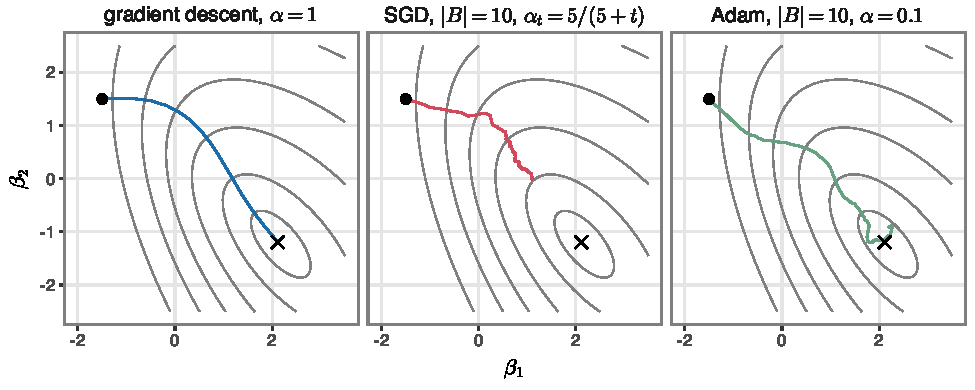
\includegraphics[width=\linewidth]{sgd_paths.pdf}
  \caption{150 iterations of three optimizers on the logistic regression loss for simulated data ($N=1000$, two features, no intercept), starting from the black dot; grey lines are loss contours and the cross marks the minimum. Gradient descent uses all $N$ samples per step and follows a smooth path. SGD and Adam use minibatches of 10 samples, so each step costs 1\% as much but the paths are noisy.}
  \label{fig:sgd}
\end{figure}

%======================================================================
\section{Gene regulation}
\label{sec:generegulation}
%======================================================================

Chapter 1 defined a gene's expression as the number of RNA copies of the gene in a cell, and gene regulation as the control of \emph{when} (for example at different stages of development), \emph{where} (in which tissues and cell types) and \emph{why} (in response to which stimuli) a gene is expressed. We now turn to \emph{how} cells achieve this. There are several reasons to care.
\begin{itemize}
  \item \emph{Basic biology}. Every cell in the body has essentially the same genome, yet a neuron, a liver cell and a muscle cell behave very differently. Much of the difference comes from which genes are expressed, and so from how the same DNA sequence is read out differently in each cell type.
  \item \emph{Understanding disease}. Most genetic variants associated with disease risk lie outside protein-coding sequence and are thought to act by changing gene regulation. Cancers and other diseases often involve regulatory programs that have gone wrong.
  \item \emph{Bioengineering}. Gene therapies are safer if the therapeutic gene is active only in the target cell type, which requires designing regulatory DNA sequence with the desired activity.
\end{itemize}

\subsection{Transcription and transcription factors}

Transcription is the synthesis of an RNA copy of a gene from its DNA template (Figure~\ref{fig:transcription}). A gene starts at the \emph{transcription start site} (TSS) and ends at the \emph{transcription end site} (TES). The enzyme that transcribes protein-coding genes is RNA polymerase II (Pol II). Pol II is recruited to the DNA near the TSS (initiation), separates the two strands and moves along the template strand, synthesizing RNA from its $5'$ end (elongation), until it stops and releases the RNA (termination). Pol II needs the help of many other proteins.

Of these, the \emph{transcription factors} (TFs) are the most important for regulation. A TF is a protein with a DNA-binding domain that gives it an affinity for particular short DNA sequences. Humans have about 1,600 TFs~\citep{lambert2018}. Activating TFs bind near a gene and help recruit Pol II, increasing transcription; repressive TFs block Pol II or other TFs, decreasing it. Binding is dynamic: a TF binds, falls off and rebinds, and many TFs with different preferences compete for access to the DNA, so binding at any one site is stochastic. A TF typically regulates hundreds of genes, which lets a cell switch whole programs on together. For example, during an immune response, TFs activated by the infection signal upregulate the genes needed to fight it.

The sequences that a TF prefers are called its \emph{motif}. A motif is a short pattern, typically 6--20 base pairs (bp), such as GATA for the GATA family of TFs. TF binding sites are found in the promoter, the region immediately upstream of the TSS, and in \emph{enhancers}, regulatory regions that can be thousands of base pairs from the gene they regulate. Chapter 3 discusses enhancers and chromatin in more detail.

\begin{figure}[t]
  \centering
  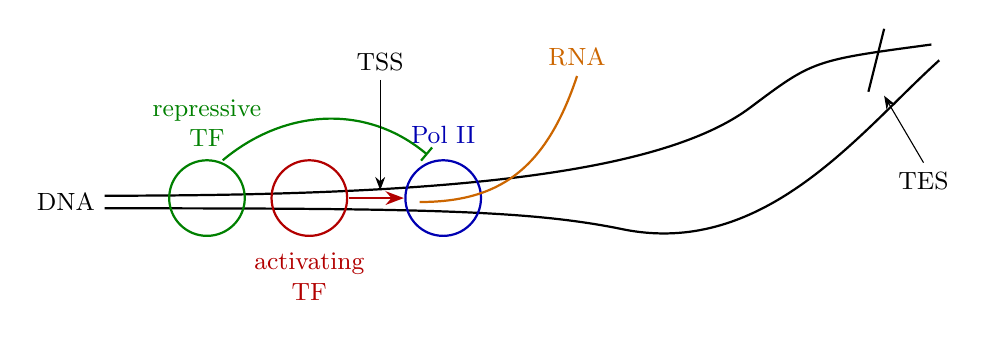
\begin{tikzpicture}[>=Stealth, every node/.style={font=\small}]
    \draw[thick] (0,0.08) .. controls (4,0.08) and (7,0.3) .. (8.2,1.2) .. controls (9,1.8) .. (10.5,2.0);
    \draw[thick] (0,-0.08) .. controls (4,-0.08) and (5.4,-0.1) .. (6.6,-0.35) .. controls (8.4,-0.7) and (9.6,0.9) .. (10.6,1.8);
    \node[left] at (0,0) {DNA};
    \draw[green!50!black, thick] (1.3,0.05) circle (0.48); \node[green!50!black, align=center] at (1.3,1.0) {repressive\\TF};
    \draw[red!70!black, thick] (2.6,0.05) circle (0.48); \node[red!70!black, align=center] at (2.6,-0.95) {activating\\TF};
    \draw[blue!70!black, thick] (4.3,0.05) circle (0.48); \node[blue!70!black] at (4.3,0.85) {Pol II};
    \draw[->, red!70!black, thick] (3.1,0.05) -- (3.8,0.05);
    \draw[-|, green!50!black, thick] (1.5,0.53) to[out=40, in=140] (4.1,0.6);
    \draw[->] (3.5,1.55) node[above] {TSS} -- (3.5,0.15);
    \draw[orange!80!black, thick] (4.0,0.0) .. controls (5.0,0.0) and (5.6,0.4) .. (6.0,1.6) node[above] {RNA};
    \draw[thick] (9.7,1.4) -- (9.9,2.2);
    \draw[->] (10.4,0.5) node[below, align=center] {TES} -- (9.9,1.35);
  \end{tikzpicture}
  \caption{Transcriptional regulation. RNA polymerase II (Pol II) binds near the transcription start site (TSS), separates the DNA strands and synthesizes RNA until the transcription end site (TES). Activating transcription factors bound nearby recruit Pol II; repressive transcription factors block it.}
  \label{fig:transcription}
\end{figure}

%======================================================================
\section{Measuring transcription factor binding with ChIP-seq}
\label{sec:chipseq}
%======================================================================

\subsection{The assay}

Chromatin immunoprecipitation followed by sequencing (ChIP-seq)~\citep{johnson2007,park2009} measures where in the genome a chosen protein is bound. \emph{Chromatin} is DNA together with the proteins bound to it. Like RNA-seq in Chapter 1, ChIP-seq converts the quantity of interest into DNA fragments that can be sequenced (Figure~\ref{fig:chipseq_protocol}).
\begin{enumerate}
  \item \emph{Cross-linking}. Cells are treated, typically with formaldehyde, to form covalent bonds between proteins and the DNA they are touching, so that transiently bound TFs are fixed in place.
  \item \emph{Fragmentation}. The chromatin is broken into fragments of a few hundred base pairs, by sonication or enzymatic digestion.
  \item \emph{Immunoprecipitation} (IP). An antibody that recognizes the TF of interest is used to pull down the TF together with the DNA fragments cross-linked to it. Antibodies are proteins made by the immune system that bind a specific target; antibodies against many TFs are available commercially.
  \item \emph{Purification}. The cross-links are reversed and the proteins, including the antibody and TF, are digested with a protease, leaving the DNA fragments that were bound.
  \item \emph{Sequencing and alignment}. The fragments are sequenced, and the reads are aligned to the genome.
\end{enumerate}
Reads pile up where the TF was bound. One limitation is that each experiment measures one TF, with one antibody, in one cell type or condition.

\begin{figure}[t]
  \centering
  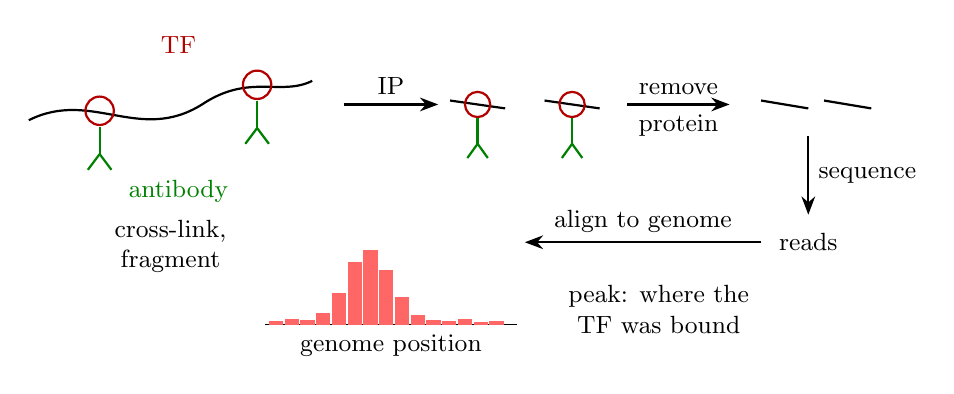
\begin{tikzpicture}[>=Stealth, every node/.style={font=\small, align=center}]
    % chromatin with TFs and antibodies
    \draw[thick] (0,0) .. controls (0.8,0.4) and (1.4,-0.3) .. (2.2,0.2) .. controls (2.8,0.6) and (3.2,0.3) .. (3.6,0.5);
    \draw[red!70!black, thick] (0.9,0.12) circle (0.18); \draw[red!70!black, thick] (2.9,0.45) circle (0.18);
    \foreach \x/\y in {0.9/0.12, 2.9/0.45} {
      \draw[green!50!black, thick] (\x,\y-0.2) -- (\x,\y-0.55); \draw[green!50!black, thick] (\x,\y-0.55) -- (\x-0.15,\y-0.75); \draw[green!50!black, thick] (\x,\y-0.55) -- (\x+0.15,\y-0.75);}
    \node[red!70!black] at (1.9,0.95) {TF};
    \node[green!50!black] at (1.9,-0.9) {antibody};
    \node at (1.8,-1.6) {cross-link,\\fragment};
    \draw[->, thick] (4.0,0.2) -- node[above] {IP} (5.2,0.2);
    % pulled-down fragments
    \foreach \x in {5.7, 6.9} {
      \draw[thick] (\x-0.35,0.25) -- (\x+0.35,0.15);
      \draw[red!70!black, thick] (\x,0.2) circle (0.16);
      \draw[green!50!black, thick] (\x,0.03) -- (\x,-0.3); \draw[green!50!black, thick] (\x,-0.3) -- (\x-0.13,-0.48); \draw[green!50!black, thick] (\x,-0.3) -- (\x+0.13,-0.48);}
    \draw[->, thick] (7.6,0.2) -- node[above] {remove} node[below] {protein} (8.9,0.2);
    \foreach \x in {9.3, 10.1} \draw[thick] (\x,0.25) -- (\x+0.6,0.15);
    \draw[->, thick] (9.9,-0.2) -- node[right] {sequence} (9.9,-1.2);
    \node at (9.9,-1.55) {reads};
    \draw[->, thick] (9.3,-1.55) -- node[above] {align to genome} (6.3,-1.55);
    % coverage
    \begin{scope}[shift={(3.0,-2.6)}]
      \draw (0,0) -- (3.2,0);
      \foreach \h [count=\k] in {0.05,0.08,0.06,0.15,0.4,0.8,0.95,0.7,0.35,0.12,0.06,0.05,0.07,0.04,0.05}
        \fill[red!60] ({0.2*\k-0.15},0) rectangle ({0.2*\k+0.03},\h);
      \node[below] at (1.6,0) {genome position};
    \end{scope}
    \node at (8.0,-2.4) {peak: where the\\TF was bound};
  \end{tikzpicture}
  \caption{ChIP-seq. Proteins are cross-linked to DNA, chromatin is fragmented, and an antibody against the transcription factor (TF) pulls down the TF with its bound DNA. After the protein is removed, the DNA is sequenced and the reads are aligned. Read coverage forms a peak where the TF was bound.}
  \label{fig:chipseq_protocol}
\end{figure}

\subsection{Peaks}

Figure~\ref{fig:igb} shows ChIP-seq data at three zoom levels. Across a whole chromosome (a), many binding sites are detected. Around a single gene (b), the read coverage is low and noisy almost everywhere, with sharp peaks at a few locations, including the TSS. At the finest scale (c), a peak spans a few hundred base pairs, the length of the sequenced fragments, and a sequence match to the TF's motif lies near its summit.

\begin{figure}[t]
  \centering
  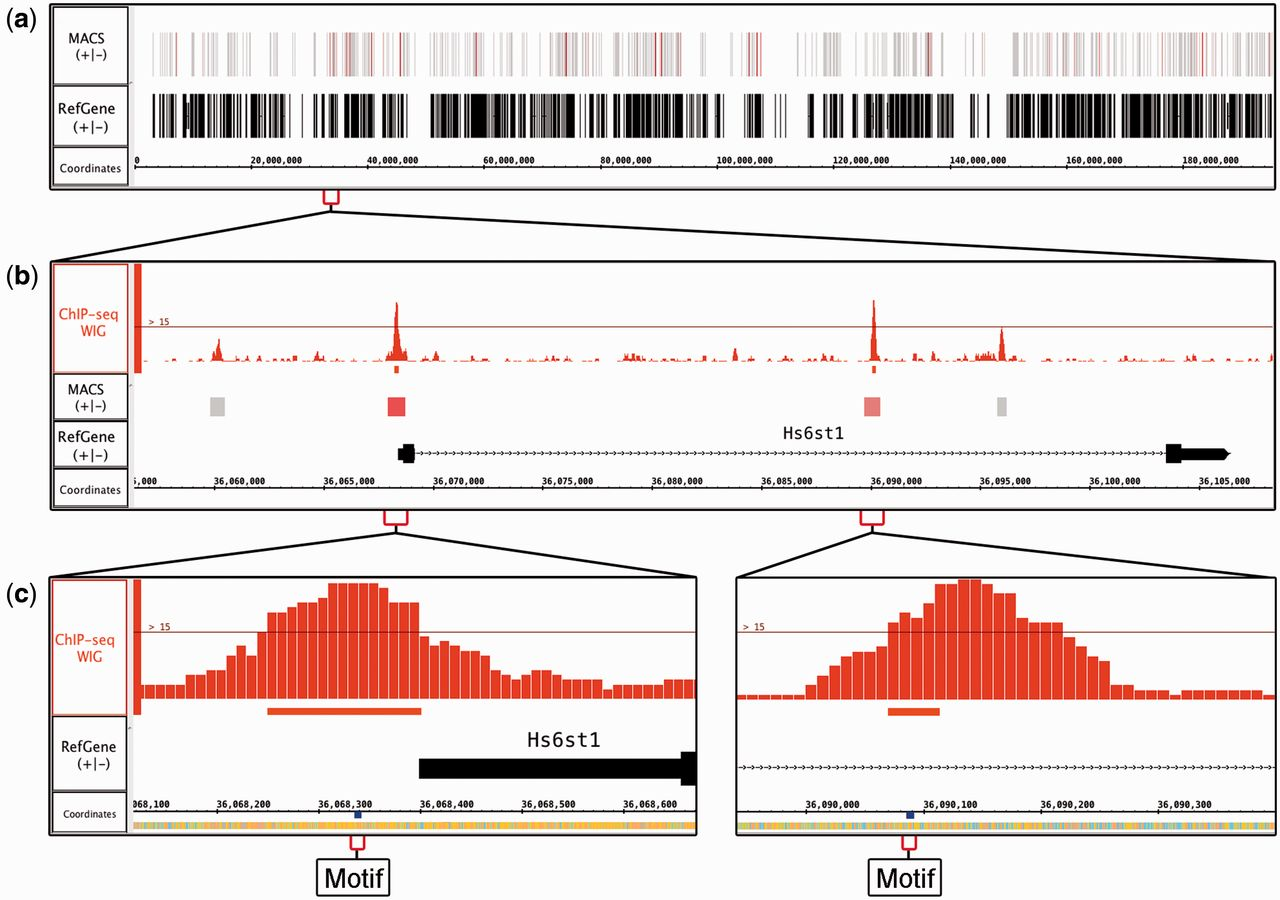
\includegraphics[width=0.85\linewidth]{slides/chipseq_igb.jpg}
  \caption{ChIP-seq data viewed in a genome browser. (a) Peaks called by MACS (top track) and genes (RefGene) along a whole chromosome. (b) Read coverage (ChIP-seq WIG track) around the gene \textit{Hs6st1}; peaks are called at the TSS and at several other sites, with grey marking lower-confidence peaks. (c) Zoom on two peaks, each a few hundred base pairs wide, with the TF's motif near the summit. Reproduced from \citet{freese2016}.}
  \label{fig:igb}
\end{figure}

\emph{Peak calling} decides where coverage is higher than expected by chance. Algorithms such as MACS~\citep{zhang2008} slide a window of width comparable to the fragment length along the genome and model the number of reads $Y$ falling in the window. Under the null hypothesis of no binding, reads land at random, so $Y\sim\text{Poisson}(\lambda)$, where $\lambda$ is the expected number of background reads in the window. The p-value for observing $y$ reads is
\begin{equation}
  \Pr(Y\geq y) = 1-\sum_{k=0}^{y-1}\frac{e^{-\lambda}\lambda^k}{k!}.
\end{equation}
For example, with $\lambda=2$, observing 15 or more reads has probability $3.9\times10^{-9}$, while with $\lambda=5$ it has probability $2.3\times10^{-4}$. Since the human genome contains about $10^7$ non-overlapping windows of 300\,bp, only the first is convincing after correcting for multiple testing. The background rate is not uniform along the genome, because some regions are easier to fragment or sequence, so MACS estimates $\lambda$ locally, using a control experiment without immunoprecipitation (``input'') where available. The output is a set of peaks, genomic intervals where the TF is inferred to bind, each with a significance score.

%======================================================================
\section{Motifs and regulatory grammar}
\label{sec:grammar}
%======================================================================

To a first approximation, a TF binds where its motif occurs. Reality is more complicated, because motifs combine~\citep{spitz2012} (Figure~\ref{fig:grammar}).
\begin{itemize}
  \item \emph{Homotypic clusters}. Regulatory sequences often contain several copies of the same motif, which together give stronger or more reliable binding than one copy.
  \item \emph{Heterotypic clusters}. Regulatory sequences are often bound by combinations of different TFs. TFs that bind next to each other can also bind each other, which stabilizes both. A well-studied example is the pair SOX2 and OCT4, which bind adjacent motifs in the regulatory regions of genes that maintain pluripotency in embryonic stem cells (Figure~\ref{fig:sox2oct4}).
  \item \emph{Spatial grammar}. For some combinations, binding or activity depends on the spacing, order and orientation of the motifs.
\end{itemize}
By analogy with language, motifs are words, and the rules by which they combine are a \emph{grammar}. Predicting where a TF binds therefore requires more than finding its motif: it requires a model of how motifs combine.

\begin{figure}[t]
  \centering
  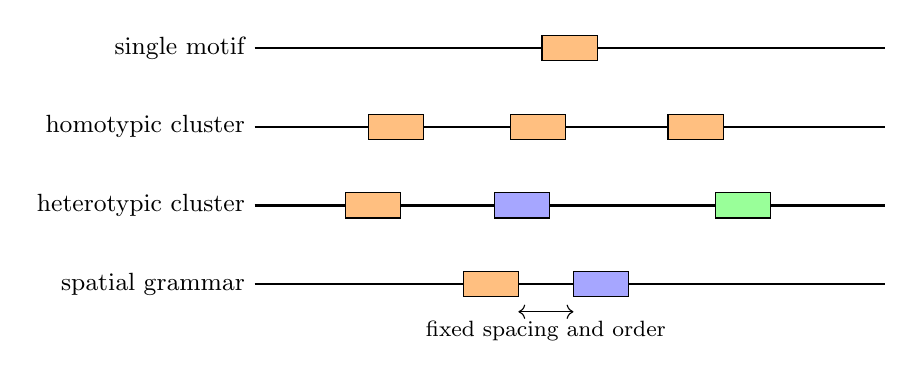
\begin{tikzpicture}[every node/.style={font=\small}, motif/.style={draw, minimum width=0.7cm, minimum height=0.32cm, inner sep=0pt}]
    \foreach \row/\lab in {0/single motif, 1/homotypic cluster, 2/heterotypic cluster, 3/spatial grammar}
      { \draw[thick] (0,-\row) -- (8,-\row); \node[left] at (0,-\row) {\lab}; }
    \node[motif, fill=orange!50] at (4,0) {};
    \foreach \x in {1.8,3.6,5.6} \node[motif, fill=orange!50] at (\x,-1) {};
    \node[motif, fill=orange!50] at (1.5,-2) {}; \node[motif, fill=blue!35] at (3.4,-2) {}; \node[motif, fill=green!40] at (6.2,-2) {};
    \node[motif, fill=orange!50] at (3.0,-3) {}; \node[motif, fill=blue!35] at (4.4,-3) {};
    \draw[<->] (3.35,-3.35) -- node[below, font=\footnotesize] {fixed spacing and order} (4.05,-3.35);
  \end{tikzpicture}
  \caption{Arrangements of transcription factor motifs (boxes; colours denote different TFs) in regulatory DNA. Homotypic clusters repeat one motif; heterotypic clusters combine motifs of different TFs; in a spatial grammar the spacing, order or orientation of the motifs matters.}
  \label{fig:grammar}
\end{figure}

\begin{figure}[t]
  \centering
  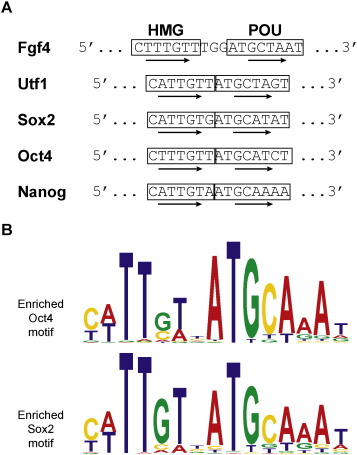
\includegraphics[width=0.4\linewidth]{slides/sox2_oct4_motifs.jpg}
  \caption{A heterotypic motif pair. (A) Adjacent SOX2 (HMG domain) and OCT4 (POU domain) binding sites in regulatory regions of five genes expressed in pluripotent stem cells. (B) Sequence logos of the motifs enriched in OCT4 and SOX2 ChIP-seq peaks, which both show the composite motif. Reproduced from \citet{rizzino2016}.}
  \label{fig:sox2oct4}
\end{figure}

\subsection{Sequence-to-function models}

ChIP-seq provides training data for a supervised learning problem (Figure~\ref{fig:seq2fun}). Take a set of DNA sequences of fixed length, for example 200--1000\,bp centred on ChIP-seq peaks (label $y=1$, bound) and an equal number from elsewhere in the genome (label $y=0$, unbound). The task is to learn a function $F$ from a sequence $S$ to the probability that the TF binds it. There are two motivations.
\begin{enumerate}
  \item \emph{Understanding}: what sequence features determine binding, and how do TFs cooperate?
  \item \emph{Prediction of variant effects}: if a mutation in a tumour or a genetic variant associated with a disease changes a regulatory sequence, does it change binding? Applying $F$ to the reference and the altered sequence answers this without a new experiment.
\end{enumerate}
The rest of this chapter develops two choices of $F$: the classical position weight matrix and the convolutional neural network.

\begin{figure}[t]
  \centering
  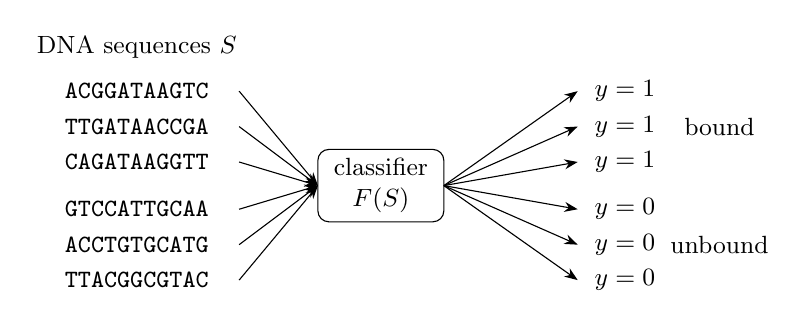
\begin{tikzpicture}[>=Stealth, every node/.style={font=\small}]
    \foreach \s/\y/\l in {ACGGATAAGTC/0.9/1, TTGATAACCGA/0.45/1, CAGATAAGGTT/0/1, GTCCATTGCAA/-0.6/0, ACCTGTGCATG/-1.05/0, TTACGGCGTAC/-1.5/0}
      { \node[font=\ttfamily\small] at (0,\y) {\s}; \node at (6.2,\y) {$y=\l$}; \draw[->] (1.3,\y) -- (2.3,-0.3); \draw[->] (3.9,-0.3) -- (5.6,\y); }
    \node[draw, rounded corners, minimum width=1.6cm, minimum height=0.9cm, align=center] at (3.1,-0.3) {classifier\\$F(S)$};
    \node at (0,1.45) {DNA sequences $S$};
    \node[align=center] at (7.4,0.45) {bound};
    \node[align=center] at (7.4,-1.05) {unbound};
  \end{tikzpicture}
  \caption{Predicting transcription factor binding as binary classification. Sequences under ChIP-seq peaks are labelled bound and sequences elsewhere unbound; a classifier $F$ maps sequence to the probability of binding.}
  \label{fig:seq2fun}
\end{figure}

%======================================================================
\section{Position weight matrices}
\label{sec:pwm}
%======================================================================

Before neural networks, TF binding was modelled with \emph{position weight matrices} (PWMs)~\citep{stormo2000}. A PWM is a simple probabilistic model that will turn out to be the first layer of a CNN.

\subsection{A probabilistic model of bound sequences}

Consider sequences of a fixed length $K$, typically between 6 and 20. Write a sequence as $x=(x_1,\dots,x_K)$ with $x_k\in\{\mathrm{A},\mathrm{C},\mathrm{G},\mathrm{T}\}$, and let $b\in\{0,1\}$ indicate whether the TF binds it ($b=1$) or not ($b=0$). We build two models for the sequence, one for bound and one for unbound sequences, and combine them with Bayes' rule.

For bound sequences, assume that the nucleotides at different positions are independent, but not identically distributed: each position $k$ has its own distribution over the four nucleotides. Let $\mP\in[0,1]^{4\times K}$ be the \emph{position probability matrix}, with rows indexed by nucleotide $n$ and columns by position $k$,
\begin{equation}
  P_{n,k} = \Pr(x_k=n\mid b=1), \qquad \sum_{n}P_{n,k}=1 .
\end{equation}
Each column of $\mP$ is a probability vector. By independence across positions,
\begin{equation}
  \Pr(x\mid b=1) = \prod_{k=1}^K\Pr(x_k\mid b=1) = \prod_{k=1}^K P_{x_k,k},
\end{equation}
where $P_{x_k,k}$ is the entry in the row of the nucleotide actually present at position $k$ and the column of position $k$. For unbound sequences we use a \emph{background} model in which every position has the same distribution $q_n$, usually the uniform $q_n=\frac14$ (or the genome-wide nucleotide frequencies),
\begin{equation}
  \Pr(x\mid b=0) = \prod_{k=1}^K q_{x_k} = \left(\tfrac14\right)^K .
\end{equation}

Let $\pi=\Pr(b=1)$ be the prior probability of binding. By Bayes' rule and the law of total probability, $\Pr(x)=\Pr(x\mid b=1)\pi+\Pr(x\mid b=0)(1-\pi)$, so
\begin{equation}
  \Pr(b=1\mid x) = \frac{\Pr(x\mid b=1)\,\pi}{\Pr(x\mid b=1)\,\pi + \Pr(x\mid b=0)\,(1-\pi)} .
\end{equation}
Dividing numerator and denominator by $\Pr(x\mid b=0)(1-\pi)$ gives
\begin{equation}
  \Pr(b=1\mid x) = \frac{\operatorname{odds}(x)}{\operatorname{odds}(x)+1}, \qquad \operatorname{odds}(x) = \frac{\Pr(b=1\mid x)}{\Pr(b=0\mid x)} = \frac{\Pr(x\mid b=1)}{\Pr(x\mid b=0)}\cdot\frac{\pi}{1-\pi} .
  \label{eq:odds}
\end{equation}
Taking logarithms to base 2, as is conventional for PWMs, the product over positions becomes a sum,
\begin{equation}
  \log_2\operatorname{odds}(x) = \sum_{k=1}^K\log_2\frac{P_{x_k,k}}{q_{x_k}} + \log_2\frac{\pi}{1-\pi} = \sum_{k=1}^K W_{x_k,k} + w_0 ,
  \label{eq:logodds}
\end{equation}
where $w_0=\log_2\frac{\pi}{1-\pi}$ and $\mW\in\R^{4\times K}$, with
\begin{equation}
  W_{n,k} = \log_2\frac{P_{n,k}}{q_n},
\end{equation}
is the \emph{position weight matrix}. $W_{n,k}>0$ means nucleotide $n$ is more common at position $k$ of bound sequences than in the background. With an uninformative prior, $\pi=\frac12$, $w_0=0$. Scoring a sequence then needs only a lookup and a sum: for each position, take the entry of $\mW$ for the nucleotide present and add them up. Sums of logs are also numerically better behaved than products of many small probabilities.

\subsection{Estimating the PWM}

Given $N_b$ aligned bound sequences of length $K$, let $C_{n,k}$ be the number of sequences with nucleotide $n$ at position $k$. The matrix of counts is the \emph{position frequency matrix}. The maximum likelihood estimate of each column of $\mP$ is the vector of observed proportions, $\hat P_{n,k}=C_{n,k}/N_b$. Table~\ref{tab:pwm_example} works through a toy example with ten bound sequences of length nine,
\begin{center}
\texttt{GAGGTAAAC\ TCCGTAAGT\ CAGGTTGGA\ ACAGTCAGT\ TAGGTCATT}\\
\texttt{TAGGTACTG\ ATGGTAACT\ CAGGTATAC\ TGTGTGAGT\ AAGGTAAGT}.
\end{center}
A nucleotide never observed at a position gets $\hat P_{n,k}=0$ and $W_{n,k}=-\infty$, so any sequence containing it has zero probability of being bound. This is too strong a conclusion from ten sequences. In practice a pseudocount $a>0$ is added, $\hat P_{n,k}=(C_{n,k}+a)/(N_b+4a)$, which is the posterior mean under a symmetric Dirichlet prior on each column.

\begin{table}[t]
  \centering
  \caption{Position frequency, probability and weight matrices (background $q_n=\frac14$, no pseudocount) for the ten toy bound sequences in the text, after the example in Wikipedia's ``Position weight matrix'' article.}
  \label{tab:pwm_example}
  \small
  \input{figures/pwm_example_table}
\end{table}

Now score the sequence $x=\texttt{GAGGTAAAC}$. Under the bound model, reading the probabilities of the nucleotides present from Table~\ref{tab:pwm_example},
\begin{equation}
  \Pr(x\mid b=1) = 0.1\times0.6\times0.7\times1.0\times1.0\times0.6\times0.7\times0.2\times0.2 = 7.056\times10^{-4},
\end{equation}
and under the background $\Pr(x\mid b=0)=(1/4)^9=3.81\times10^{-6}$. With $\pi=\frac12$ the odds are $7.056\times10^{-4}/3.81\times10^{-6}=185$, and $\Pr(b=1\mid x)=185/186=0.995$. The same answer comes from the PWM by addition,
\begin{equation}
  \log_2\operatorname{odds}(x) = -1.32+1.26+1.49+2.00+2.00+1.26+1.49-0.32-0.32 = 7.53,
\end{equation}
and $2^{7.53}=185$.

\subsection{The PWM model is logistic regression}

Equation~\eqref{eq:odds} gives $\Pr(b=1\mid x)=1/(1+2^{-s})=\sigma(s\ln 2)$, where $s=\log_2\operatorname{odds}(x)$ and $\sigma$ is the logistic function. Represent the sequence by its \emph{one-hot encoding} $\mX\in\{0,1\}^{4\times K}$, with $X_{n,k}=1$ if $x_k=n$ and 0 otherwise. Each column has a single 1, so $W_{x_k,k}=\sum_nW_{n,k}X_{n,k}$ and
\begin{equation}
  s = \sum_{k=1}^K\sum_{n}W_{n,k}X_{n,k} + w_0 ,
  \label{eq:pwm_linear}
\end{equation}
a linear function of the $4K$ one-hot features. The PWM model is therefore a logistic regression on the one-hot encoded sequence, with coefficients $\mW\ln 2$ and intercept $w_0\ln 2$. The classical approach estimates $\mW$ \emph{generatively}, from the nucleotide counts in bound sequences only. We could instead fit the same model \emph{discriminatively}, by maximizing the logistic regression likelihood of bound and unbound sequences as in Chapter 1. A neural network does the latter.

\subsection{Sequence logos}

PWMs are visualized as \emph{sequence logos}~\citep{schneider1990} (Figure~\ref{fig:logos}). The most common form plots at each position a stack of letters whose total height is the \emph{information content}
\begin{equation}
  I_k = \log_2 4 - \left(-\sum_{n}P_{n,k}\log_2P_{n,k}\right) = 2+\sum_n P_{n,k}\log_2 P_{n,k}
\end{equation}
bits, the reduction in entropy relative to a uniform distribution, with each letter's height proportional to $P_{n,k}$. A position where one nucleotide always occurs has $I_k=2$ bits; a position with a uniform distribution has $I_k=0$ and is invisible. With a uniform background, $I_k=\sum_nP_{n,k}\log_2(P_{n,k}/\frac14)=\sum_nP_{n,k}W_{n,k}$: the information content is the expected PWM score of position $k$ for a bound sequence, which is the Kullback--Leibler divergence of the position's distribution from the background. Logos can also show the weights $W_{n,k}$ directly, with positive weights above the axis and negative weights below. Figure~\ref{fig:logos}b uses this form for an illustrative PWM for the GATA family of TFs, whose core positions spell GATA (the consensus GATA site is usually written (A/T)GATA(A/G)); Table~\ref{tab:pwm_scan} lists its weights.

\begin{figure}[t]
  \centering
  \begin{subfigure}[b]{0.48\linewidth}
    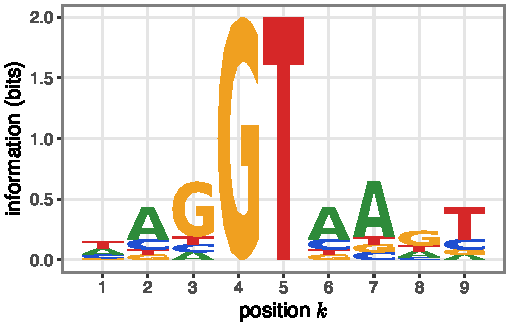
\includegraphics[width=\linewidth]{logo_wiki.pdf}
    \caption{}
  \end{subfigure}\hfill
  \begin{subfigure}[b]{0.48\linewidth}
    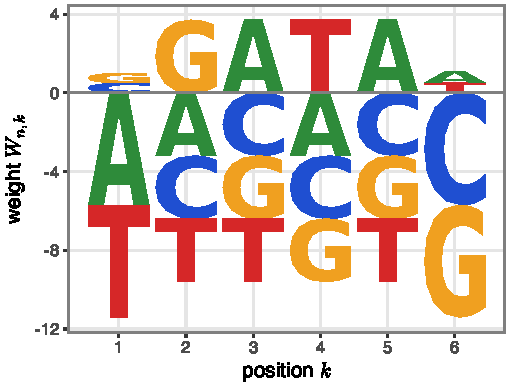
\includegraphics[width=\linewidth]{logo_gata.pdf}
    \caption{}
  \end{subfigure}
  \caption{Sequence logos. (a) Information-content logo of the toy motif in Table~\ref{tab:pwm_example}: letter heights are $P_{n,k}I_k$. Positions 4 and 5 are invariant (2 bits). (b) Weight logo of the GATA PWM used in the text (log-odds units): letter heights are $W_{n,k}$, with negative weights below the axis.}
  \label{fig:logos}
\end{figure}

\subsection{Scanning a longer sequence}

A ChIP-seq peak is hundreds of base pairs long, while a motif is a few base pairs, and the motif can be anywhere in the peak. To find it we \emph{scan} the PWM along the sequence. Let $\mX\in\{0,1\}^{4\times L}$ be the one-hot encoding of a sequence of length $L>K$. The score of the window starting at position $j$ is, by~\eqref{eq:pwm_linear},
\begin{equation}
  z_j = \sum_{k=1}^{K}\sum_{n}W_{n,k}X_{n,j+k-1}, \qquad j=1,\dots,L-K+1 ,
  \label{eq:scan}
\end{equation}
the sum of the elementwise product of $\mW$ with the $4\times K$ block of $\mX$ starting at column $j$. The one-hot zeros cancel every weight except the one for the nucleotide present. To keep the output the same length as the input, the sequence can be \emph{padded} with columns of zeros at each end, which contribute nothing to the score. Table~\ref{tab:pwm_scan} scans the six-position GATA PWM along a 13\,bp sequence, padded with two zero columns on the left and three on the right. The window \texttt{CGATAA} matches the motif and scores 15.9; every other window scores at most 2.1.

\begin{table}[t]
  \centering
  \caption{Scanning the GATA PWM (top, rows A, C, G, T; positions 1--6) along the one-hot encoded sequence \texttt{GCATTACCGATAA}, padded with two columns of zeros on the left and three on the right, so that score $z_j$ is for the window covering positions $j-2$ to $j+3$. ReLU sets negative scores to zero. Max pooling with width 4 and stride 4 keeps the largest score in each block of four, discarding the last position; applying ReLU after pooling gives the same result as before, 2.1, 0 and 15.9.}
  \label{tab:pwm_scan}
  \small
  \begin{tabular}{l*{6}{r}}
    \toprule
    PWM $\mW$ & 1 & 2 & 3 & 4 & 5 & 6 \\
    \midrule
    A & $-5.7$ & $-3.2$ & $3.7$ & $-3.2$ & $3.7$ & $0.6$ \\
    C & $0.5$ & $-3.2$ & $-3.2$ & $-3.2$ & $-3.2$ & $-5.7$ \\
    G & $0.5$ & $3.7$ & $-3.2$ & $-3.2$ & $-3.2$ & $-5.7$ \\
    T & $-5.7$ & $-3.2$ & $-3.2$ & $3.7$ & $-3.2$ & $0.5$ \\
    \bottomrule
  \end{tabular}\\[1em]
  \setlength{\tabcolsep}{3.5pt}
  \input{figures/pwm_scan_table}
\end{table}

DNA is double stranded and a TF can bind its motif on either strand. A match on the reverse strand appears in the forward sequence as the reverse complement of the motif, so in practice the sequence is scanned with both $\mW$ and its reverse complement, obtained by reversing the columns of $\mW$ and swapping the A and T rows and the C and G rows.

\subsection{Limitations: the futility theorem}

PWM scanning finds far more matches than there are binding sites. A specific 6\,bp sequence occurs by chance once every $4^6=4096$\,bp on each strand, so about $2\times3.1\times10^9/4096\approx1.5\times10^6$ times in the human genome, whereas a ChIP-seq experiment typically finds $10^3$--$10^5$ binding sites for a TF. \citet{wasserman2004} called this the \emph{futility theorem}: nearly all predicted sites are not bound. A single motif score ignores the cooperating TFs and the grammar described in Section~\ref{sec:grammar}, and the accessibility of the DNA, which is the topic of Chapter 3. We need a model that can learn several motifs and how they combine.

%======================================================================
\section{Convolutional neural networks}
\label{sec:cnn}
%======================================================================

\subsection{A PWM is a convolutional filter}

The scan~\eqref{eq:scan} is exactly the operation performed by the first layer of a one-dimensional CNN. In deep learning terminology, $\mW$ is a \emph{filter} or \emph{kernel}, the four rows of the one-hot input are \emph{channels} (as the red, green and blue channels of an image), and $z_j$ is the \emph{activation} of a unit at position $j$. Two things change. First, the weights are not estimated from counts but learned, like any other neural network weights, by SGD on the loss for predicting binding. Second, the network uses many filters, so it can detect several motifs, and it stacks further layers on top to model how they combine. The first-layer filters are usually initialized at random rather than from known PWMs, although initializing them from motif databases has been tried.

\subsection{Convolution layers}

Start with a single input channel $x_1,\dots,x_L$ and a filter $w_1,\dots,w_K$. The output is
\begin{equation}
  y_j = \sum_{k=1}^{K}w_k\,x_{j+k-1}, \qquad j=1,\dots,L-K+1 .
\end{equation}
With $C_{\text{in}}$ input channels, $\mX\in\R^{C_{\text{in}}\times L}$, the filter has a weight for every channel and offset, $\mW\in\R^{C_{\text{in}}\times K}$, and the products are summed over channels as well, $y_j=\sum_{k}\sum_{c}W_{c,k}X_{c,j+k-1}$. For DNA, $C_{\text{in}}=4$ and this is the PWM scan. Finally, with $C_{\text{out}}$ filters, each producing one output channel,
\begin{equation}
  Y_{d,j} = b_d + \sum_{k=1}^{K}\sum_{c=1}^{C_{\text{in}}}W_{d,c,k}\,X_{c,j+k-1}, \qquad d=1,\dots,C_{\text{out}},
  \label{eq:conv}
\end{equation}
where $b_d$ is a bias for filter $d$. The weights form a three-dimensional array (a \emph{tensor}) and the shapes are
\begin{equation}
  \mW: [C_{\text{out}}\times C_{\text{in}}\times K], \qquad \mX: [C_{\text{in}}\times L], \qquad \mY: [C_{\text{out}}\times(L-K+1)].
\end{equation}
Each output channel is the scan of one PWM-like filter, for example one for each of several TFs. A nonlinearity is applied elementwise to $\mY$, and the result is the input to the next layer, which has $C_{\text{out}}$ input channels.

Mathematically, the convolution of two functions is $(f*g)(t)=\int f(t-\tau)g(\tau)\,d\tau$, and its discrete version $\sum_kw_kx_{j-k}$ runs through the filter backwards. Equation~\eqref{eq:conv} does not reverse the filter, so strictly it is a \emph{cross-correlation}. Deep learning libraries implement cross-correlation and call it convolution. Since the filter is learned, the distinction does not matter.

The key property of a convolution layer is \emph{weight sharing}: the same filter is applied at every position. A motif detector learned from a GATA site near the start of one training sequence also detects GATA sites anywhere else. Sharing also keeps the number of parameters small, $C_{\text{out}}C_{\text{in}}K+C_{\text{out}}$, independent of the sequence length. A dense layer connecting a 1000\,bp one-hot input to the same number of hidden units would need a separate weight for every position. Because each weight is used at every position, its gradient is a sum over positions: by the chain rule applied to~\eqref{eq:conv},
\begin{equation}
  \frac{\partial\ell}{\partial W_{d,c,k}} = \sum_{j}\frac{\partial\ell}{\partial Y_{d,j}}\,X_{c,j+k-1}.
\end{equation}

\subsection{Padding, stride and dilation}

Three options control which positions a filter visits (Figure~\ref{fig:conv_arith}).
\begin{itemize}
  \item \emph{Padding} $p$ adds $p$ columns of zeros to each end of the input, so that the filter can be centred near the ends. Without padding the output is $K-1$ positions shorter than the input; with stride 1, odd $K$ and $p=(K-1)/2$ (``same'' padding) the output has the same length as the input.
  \item \emph{Stride} $s$ moves the filter $s$ positions at a time rather than one, which shortens the output by a factor of about $s$.
  \item \emph{Dilation} $\delta$ spaces the $K$ filter weights $\delta$ positions apart, so the filter spans $\delta(K-1)+1$ positions with only $K$ weights. We will use it for long-range models in later chapters.
\end{itemize}
The output length follows by counting where the filter can start. The padded input has length $L+2p$ and the filter spans $\delta(K-1)+1$ positions, so the filter's first weight can sit at positions $1,\dots,L+2p-\delta(K-1)$. With stride $s$ it visits positions $1,1+s,1+2s,\dots$, and the number of these not exceeding $L+2p-\delta(K-1)$ is
\begin{equation}
  L_{\text{out}} = \left\lfloor\frac{L+2p-\delta(K-1)-1}{s}\right\rfloor + 1,
  \label{eq:lout}
\end{equation}
where $\lfloor\cdot\rfloor$ rounds down. For the three cases in Figure~\ref{fig:conv_arith}, with $L=5$, $K=3$ and $\delta=1$: $p=0,s=1$ gives $\lfloor 2/1\rfloor+1=3$; $p=1,s=1$ gives $\lfloor4/1\rfloor+1=5$; and $p=1,s=2$ gives $\lfloor4/2\rfloor+1=3$. For genomic sequence, a stride of 1 in convolution layers is usually recommended, since a stride larger than one evaluates the filter only at every $s$-th position and can step over a motif; downsampling is better done by pooling.

\begin{figure}[t]
  \centering
  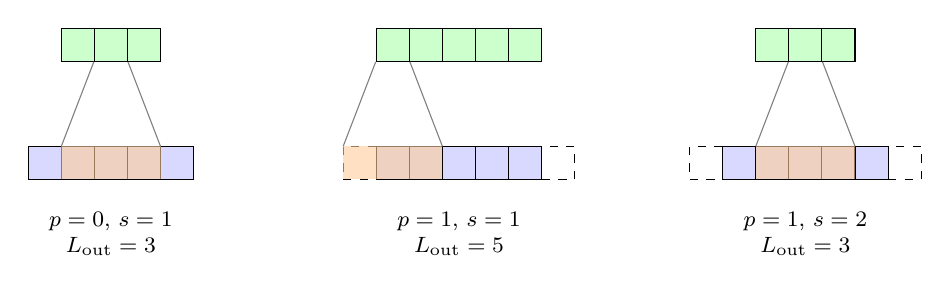
\begin{tikzpicture}[every node/.style={font=\small}, cell/.style={draw, minimum size=0.42cm, inner sep=0pt}, pad/.style={draw, dashed, minimum size=0.42cm, inner sep=0pt}]
    \newcommand{\convpanel}[6]{% x-shift, padding, stride, n-out, title, highlighted-out
      \begin{scope}[xshift=#1cm]
        \foreach \i in {1,...,5} \node[cell, fill=blue!15] (in\i) at ({0.42*(\i+#2)},0) {};
        \ifnum#2>0 \node[pad] (in0) at (0.42,0) {}; \node[pad] (in6) at ({0.42*(6+#2)},0) {}; \fi
        \foreach \j in {1,...,#4} \node[cell, fill=green!20] (out\j) at ({0.42*(#2+5+1+#2)/2 + 0.42*(\j-(#4+1)/2)},1.5) {};
        \fill[orange!40, opacity=0.6] ({0.42*(1+(#6-1)*#3)-0.21},-0.21) rectangle ({0.42*(3+(#6-1)*#3)+0.21},0.21);
        \draw[gray] ({0.42*(1+(#6-1)*#3)-0.21},0.21) -- (out#6.south west);
        \draw[gray] ({0.42*(3+(#6-1)*#3)+0.21},0.21) -- (out#6.south east);
        \node[align=center, font=\footnotesize] at ({0.42*(5+2*#2+1)/2},-0.9) {#5};
      \end{scope}}
    \convpanel{0}{0}{1}{3}{$p=0$, $s=1$\\$L_{\text{out}}=3$}{2}
    \convpanel{4.0}{1}{1}{5}{$p=1$, $s=1$\\$L_{\text{out}}=5$}{1}
    \convpanel{8.4}{1}{2}{3}{$p=1$, $s=2$\\$L_{\text{out}}=3$}{2}
  \end{tikzpicture}
  \caption{One-dimensional convolution of an input of length $L=5$ (blue, bottom) with a filter of width $K=3$, for three settings of padding $p$ (dashed cells are zeros) and stride $s$. The shaded window produces the connected output (green, top). With several channels the same picture applies to every channel and the products are summed across channels. After the two-dimensional illustrations of \citet{dumoulin2016}.}
  \label{fig:conv_arith}
\end{figure}

\subsection{Thresholding and pooling}

Recall that a log-odds score $z_j>0$ means binding is more likely than not. A natural step is to \emph{threshold} the scores, setting negative scores to zero (no motif) and keeping positive scores as a measure of match strength. This is the ReLU, $\max(z_j,0)$, applied after the convolution (Table~\ref{tab:pwm_scan}).

\emph{Max pooling} then summarizes the activations over local windows. With pool width $w$ and stride $s$, applied to each channel separately,
\begin{equation}
  Y_{c,j} = \max_{k=1,\dots,w} Z_{c,(j-1)s+k}.
\end{equation}
In Table~\ref{tab:pwm_scan}, pooling with $w=s=4$ reduces 13 scores to 3. Since the ReLU and the maximum are both nondecreasing, $\max_k\operatorname{ReLU}(z_k)=\operatorname{ReLU}(\max_kz_k)$, so it does not matter whether the ReLU is applied before or after pooling. Pooling has three effects.
\begin{itemize}
  \item \emph{Local translation invariance}. If the GATA match in Table~\ref{tab:pwm_scan} moved one position left or right within its pooling window, the pooled output would not change. For binding, the exact position of a motif within a few base pairs rarely matters.
  \item \emph{Lower resolution}. Later layers see a shorter sequence summarizing where motifs occur at coarser resolution, and each of their units covers a longer stretch of the input.
  \item \emph{Efficiency}. Later layers are cheaper to compute.
\end{itemize}
During backpropagation, the gradient of a pooled output passes only to the input that achieved the maximum.

\subsection{A CNN for transcription factor binding}

A typical CNN for sequence alternates convolution, ReLU and max pooling a few times, then \emph{flattens} the final channels-by-positions array into a vector and passes it to a dense MLP whose output is the probability of binding. This design follows early successful image models such as LeNet~\citep{lecun1998} and AlexNet~\citep{krizhevsky2012}. Figure~\ref{fig:cnn} shows a small example on a 12\,bp input.
\begin{enumerate}
  \item Input: one-hot sequence, $4\times12$.
  \item Convolution 1: 3 filters of width 5, stride 1, no padding, then ReLU: $3\times8$. Each filter is a learned PWM.
  \item Max pooling, width 2, stride 2: $3\times4$.
  \item Convolution 2: 2 filters of width 3 over the 3 channels, then ReLU: $2\times2$. Each filter detects a combination of first-layer motifs at particular relative positions, a piece of grammar.
  \item Flatten to a vector of length 4; dense layer to 3 hidden units with ReLU; dense layer to one output; logistic sigmoid gives $\Pr(\text{TF bound}\mid\mX)$.
\end{enumerate}
Using~\eqref{eq:lout}, the lengths are $12-5+1=8$, $\lfloor(8-2)/2\rfloor+1=4$ and $4-3+1=2$. The network has $3\cdot4\cdot5+3=63$ parameters in the first convolution, $2\cdot3\cdot3+2=20$ in the second, $4\cdot3+3=15$ in the first dense layer and $3+1=4$ in the output layer. The \emph{receptive field} of a unit is the stretch of input it depends on: 5\,bp for the first convolution, 6\,bp after pooling (two adjacent windows of 5), and $6+2\times2=10$\,bp for the second convolution, whose three inputs are pooled units spaced 2\,bp apart. Real models take inputs of hundreds to thousands of base pairs and use hundreds of filters in each layer, but the structure is the same.

\begin{figure}[t]
  \centering
  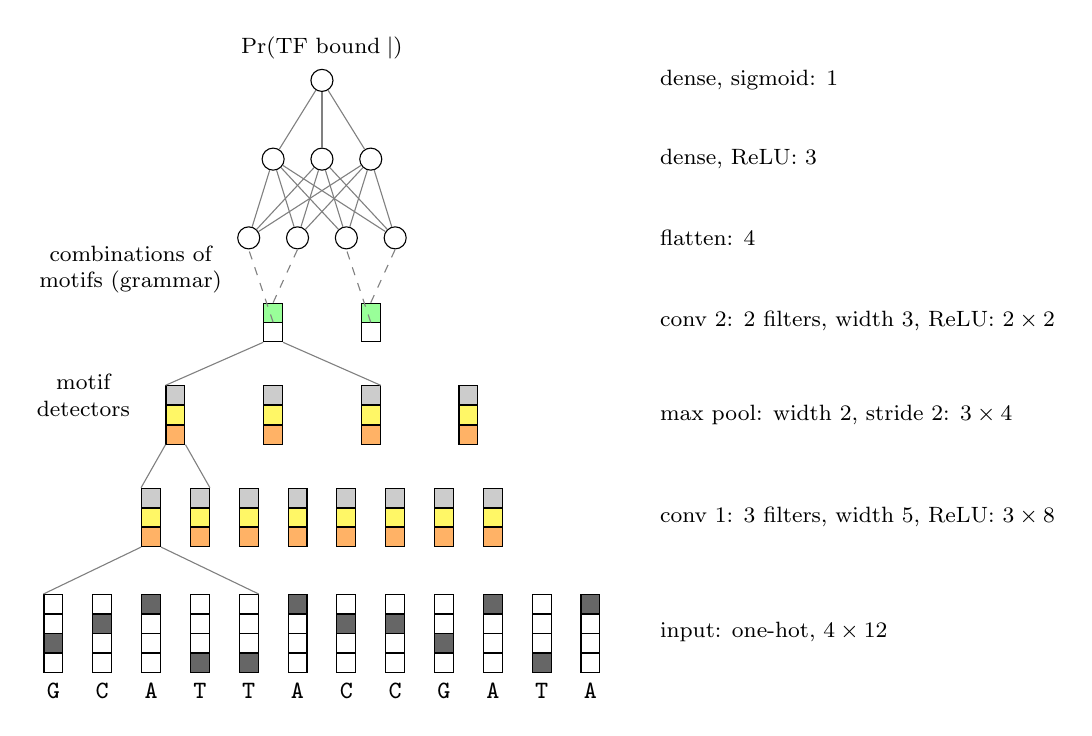
\begin{tikzpicture}[>=Stealth, every node/.style={font=\footnotesize},
      sq/.style={draw, minimum size=0.24cm, inner sep=0pt}]
    \def\dx{0.62}
    % input: 12 positions x 4 channels
    \foreach \j/\b/\on in {1/G/2,2/C/3,3/A/4,4/T/1,5/T/1,6/A/4,7/C/3,8/C/3,9/G/2,10/A/4,11/T/1,12/A/4} {
      \foreach \c in {1,...,4} \node[sq] (x\j\c) at ({\dx*\j}, {0.25*(\c-1)}) {};
      \node[sq, fill=black!60] at ({\dx*\j}, {0.25*(\on-1)}) {};
      \node[font=\ttfamily\small] at ({\dx*\j},-0.35) {\b};
    }
    % conv1: 8 positions x 3 channels, at y=1.9
    \foreach \j in {1,...,8} \foreach \c/\col in {1/orange!60,2/yellow!60,3/gray!40}
      \node[sq, fill=\col] (a\j\c) at ({\dx*(\j+2)}, {1.6+0.25*(\c-1)}) {};
    \draw[gray] (x14.north west) -- (a11.south west); \draw[gray] (x54.north east) -- (a11.south east);
    % pool: 4 positions x 3 channels
    \foreach \j in {1,...,4} \foreach \c/\col in {1/orange!60,2/yellow!60,3/gray!40}
      \node[sq, fill=\col] (m\j\c) at ({\dx*(2*\j+1.5)}, {2.9+0.25*(\c-1)}) {};
    \draw[gray] (a13.north west) -- (m11.south west); \draw[gray] (a23.north east) -- (m11.south east);
    % conv2: 2 positions x 2 channels
    \foreach \j in {1,2} \foreach \c/\col in {1/white,2/green!40}
      \node[sq, fill=\col] (b\j\c) at ({\dx*(2*\j+3.5)}, {4.2+0.25*(\c-1)}) {};
    \draw[gray] (m13.north west) -- (b11.south west); \draw[gray] (m33.north east) -- (b11.south east);
    % flatten + dense
    \foreach \k in {1,...,4} \node[draw, circle, minimum size=0.28cm, inner sep=0pt] (f\k) at ({\dx*(\k+4.0)}, 5.4) {};
    \foreach \k in {1,...,3} \node[draw, circle, minimum size=0.28cm, inner sep=0pt] (d\k) at ({\dx*(\k+4.5)}, 6.4) {};
    \node[draw, circle, minimum size=0.28cm, inner sep=0pt] (out) at ({\dx*6.5}, 7.4) {};
    \foreach \k/\src in {1/b11,2/b12,3/b21,4/b22} \draw[gray, dashed] (\src.north) -- (f\k.south);
    \foreach \k in {1,...,4} \foreach \l in {1,...,3} \draw[gray] (f\k) -- (d\l);
    \foreach \l in {1,...,3} \draw[gray] (d\l) -- (out);
    \node[above] at (out.north) {$\Pr(\text{TF bound}\mid\mX)$};
    % labels
    \begin{scope}[every node/.style={font=\footnotesize, align=left, anchor=west}]
      \node at (8.2,0.4) {input: one-hot, $4\times12$};
      \node at (8.2,1.85) {conv 1: 3 filters, width 5, ReLU: $3\times8$};
      \node at (8.2,3.15) {max pool: width 2, stride 2: $3\times4$};
      \node at (8.2,4.35) {conv 2: 2 filters, width 3, ReLU: $2\times2$};
      \node at (8.2,5.4) {flatten: 4};
      \node at (8.2,6.4) {dense, ReLU: 3};
      \node at (8.2,7.4) {dense, sigmoid: 1};
    \end{scope}
    \node[align=center, font=\footnotesize] at (1.0,3.4) {motif\\detectors};
    \node[align=center, font=\footnotesize] at (1.6,5.0) {combinations of\\motifs (grammar)};
  \end{tikzpicture}
  \caption{A small CNN for predicting transcription factor binding. Each column of squares is one position and each square one channel (input rows, top to bottom: A, C, G, T; filled squares mark the nucleotide present); colours in a layer are different filters, and the same filter (same colour) is applied at every position. Grey lines show the inputs to the first unit of each layer: 5 input positions for convolution 1, 2 positions for pooling and 3 pooled positions for convolution 2. Dashed lines show the flattening of the $2\times2$ output of convolution 2 into a vector.}
  \label{fig:cnn}
\end{figure}

\subsection{A worked example}

To see how such a network can encode grammar, set its weights by hand. The input is the 13\,bp sequence \texttt{CGCATTACGATAA}, and the first convolution has three filters of width 6 with no padding, giving outputs of length 8. Filter 1 is the GATA PWM of Table~\ref{tab:pwm_scan}. Filter 2 detects the motif [C/G]ATTA[C/G], resembling the core of the motif of NANOG, another pluripotency TF, with weights $3.7$ for A at positions 2 and 5 and for T at positions 3 and 4, $-3.2$ for the other nucleotides at those positions, and weights between $-3.2$ and $2.0$ at the flanking positions 1 and 6 that favour C or G. Filter 3 has random weights centred on $-2$ and represents an unused filter. After the ReLU the three channels are
\begin{align*}
  \text{GATA:}\ & (0,\ 2.1,\ 0,\ 0,\ 0,\ 0,\ 0,\ 15.9),\\
  \text{NANOG:}\ & (0,\ 0,\ 18.0,\ 0,\ 0,\ 0,\ 0,\ 1.8),\\
  \text{filter 3:}\ & (0,\ 0,\ 0,\ 0,\ 0,\ 0,\ 0,\ 0).
\end{align*}
The NANOG-like site \texttt{CATTAC} starts at position 3 and the GATA site \texttt{CGATAA} at position 8. Max pooling with width 2 and stride 2 gives $(2.1,0,0,15.9)$ for GATA and $(0,18.0,0,1.8)$ for NANOG. The first filter of the second convolution has width 3, with weights $(-0.4,-0.2,0.7)$ on the GATA channel, $(0.6,-0.9,-1.2)$ on the NANOG channel and $(-1.1,-1.2,-1.0)$ on channel 3. Its positive weights pick out a NANOG site in the first pooled position of its window and a GATA site in the third, that is, a GATA site starting 3--5\,bp after the start of a NANOG site. At its second position, over pooled positions 2--4,
\begin{equation*}
  0.7\times15.9 + 0.6\times18.0 - 1.2\times1.8 = 19.77,
\end{equation*}
while at its first position the output is negative and the ReLU gives 0. The second filter of this layer has negative weights and outputs zeros. Flattening gives $(0,19.77,0,0)$. A dense layer with weight $0.3$ from the second element to its first hidden unit, and weights that give negative inputs to the other two hidden units, produces $(5.93,0,0)$ after the ReLU. The output weight $0.5$ on the first hidden unit gives the logit $2.97$ and $\Pr(\text{bound})=\sigma(2.97)=0.95$. If the GATA site were moved far from the NANOG site, the second-layer filter would not fire and the predicted probability would drop, even though both motifs are still present. In a trained network such weights are learned from data rather than set by hand.

\subsection{Multitask CNNs}

A network can predict several outputs at once by giving the output layer one unit per task (Figure~\ref{fig:cnn} with $D>1$ output units), for example the binding of several TFs, or of one TF in several cell types. Each output has its own sigmoid and binary cross-entropy loss, and the total loss is their sum. This is \emph{multitask learning}. All tasks share the convolutional layers, so a motif detector learned for one TF is available to the others. Multitask training sometimes improves accuracy, particularly when tasks share motifs or cofactors, but not always. DeepSEA~\citep{zhou2015}, for example, predicts 919 chromatin features, including the binding of many TFs, from 1000\,bp of sequence with a single CNN.

\subsection{Learned filters and PWMs}

The first-layer filters of a trained CNN are analogous to PWMs, and many resemble known motifs. The correspondence is loose, however.
\begin{itemize}
  \item Filters are learned from random initialization by SGD, not from counts, so their scale is arbitrary and they need not be log-probability ratios.
  \item One real motif may be represented by a combination of several filters, for example two filters covering its two halves, or several partially redundant copies. Reading motifs off individual filters is therefore unreliable, which motivates the interpretation methods of later chapters.
  \item Even to predict the binding of a single TF, a model needs more than one filter: the futility theorem says the TF's own motif is not enough, and other filters capture cofactor motifs and sequence features associated with accessible DNA.
\end{itemize}
DeepBind~\citep{alipanahi2015} and DeepSEA~\citep{zhou2015} were early CNNs of this kind for TF binding, and Basset~\citep{kelley2016} applied the same idea to chromatin accessibility. Basenji~\citep{kelley2018}, Enformer~\citep{avsec2021} and more recent models predict many regulatory measurements from much longer sequences, and SpliceAI~\citep{jaganathan2019} predicts RNA splicing from sequence. \citet{ching2018} review deep learning in biology more broadly.

%======================================================================
\section{Strengths and weaknesses of deep neural networks}
%======================================================================

Why have deep neural networks become so popular, and when should we be wary of them? Points raised in class discussion, with some additions, include the following.

Strengths:
\begin{itemize}
  \item Flexibility: they model nonlinearity and interactions without hand-crafted features, and can be scaled up by adding layers and units.
  \item Representation learning: intermediate layers learn useful features, such as motif detectors, directly from the data.
  \item Architectures encode prior knowledge. A CNN's \emph{inductive bias} of local, translation-invariant pattern detection suits sequence data.
  \item Multiple outputs and multitask learning are straightforward.
  \item Mature, well-supported software (PyTorch, TensorFlow, JAX) with automatic differentiation and hardware acceleration, and SGD scales to very large data sets.
\end{itemize}
Weaknesses:
\begin{itemize}
  \item More moving parts than a linear model, so more ways to make mistakes. The dangerous failures are silent: a leak between training and test data can produce implausibly good performance. A class project that predicted Alzheimer's disease case-control status from genotype with nearly 100\% accuracy, impossible for a trait that is only partly heritable, is a cautionary example.
  \item Computationally expensive, and overkill when a linear model suffices.
  \item Harder to interpret than sparse linear models.
  \item On tabular data, such as gene expression matrices, they are often outperformed by gradient-boosted trees~\citep{grinsztajn2022}.
  \item They need many samples. When features outnumber samples, $P>N$, as is common in Chapter 1's applications, regularized linear models usually do better. Sequence models avoid this because each training example is one of millions of genomic sequences.
\end{itemize}

A related warning concerns the inductive bias of CNNs. Convolution and pooling make sense only if the input has a meaningful spatial dimension, such as position along a sequence or in an image. The motif GATA works only if its four nucleotides are adjacent; scattering them across the input destroys the signal. Applying a CNN to a vector of gene expression values, whose order is arbitrary, imposes an inductive bias that does not match the data.

%======================================================================
\section{Summary}
%======================================================================

\begin{itemize}
  \item Linear models cannot represent nonlinear relationships or interactions without enumerating them. Neural networks stack layers of linear maps and elementwise nonlinearities such as the ReLU; without the nonlinearity, a deep network collapses to a linear model.
  \item Gradients of the loss with respect to all weights are computed by backpropagation, the chain rule applied from the loss back to the inputs. Networks are fit with stochastic gradient descent on minibatches, usually with an adaptive method such as Adam.
  \item Transcription factors are proteins that bind short DNA motifs and control how much genes are transcribed. ChIP-seq measures where a TF binds genome-wide, giving peaks of read coverage.
  \item Binding depends on combinations of motifs: homotypic and heterotypic clusters and spatial grammar.
  \item A position weight matrix is a log-odds model of binding that assumes independent positions; it is a logistic regression on the one-hot encoded sequence. Scanning a PWM along a sequence is a convolution.
  \item A CNN learns many PWM-like filters in its first layer, thresholds them with ReLUs, pools them for local translation invariance, and models how motifs combine in later layers. CNNs are appropriate when the input has a meaningful spatial structure.
\end{itemize}

%======================================================================
\section*{Exercises}
%======================================================================

\begin{enumerate}
  \item Derive the backpropagation equations for a one-hidden-layer network with ReLU hidden units, $D$ outputs, a softmax and the cross-entropy loss. Show that $\partial\ell/\partial o_d=p_d-\ind[y=d]$, where $p_d$ is the softmax probability of class $d$.
  \item Show that if the activation function is the identity, a network with $M$ hidden layers computes a linear function of its input. What is the rank of the effective coefficient matrix if one hidden layer has fewer units than both the input and the output?
  \item For the toy sequences of Table~\ref{tab:pwm_example}, recompute the PWM with a pseudocount $a=0.5$, and score \texttt{GAGGTAAAC} and \texttt{GAGCTAAAC}. Why does the second sequence have zero probability of binding without the pseudocount?
  \item Show that with a uniform background the information content $I_k$ of a PWM column equals $\sum_nP_{n,k}W_{n,k}$, and that it is the Kullback--Leibler divergence of column $k$ of $\mP$ from the background.
  \item Use~\eqref{eq:lout} to find the output length of a convolution with $L=1000$, $K=19$, $p=9$, $s=1$ and $\delta=1$, and with $\delta=4$. What padding keeps the length at 1000 for $\delta=4$?
  \item Show that max pooling commutes with any nondecreasing activation function, and give an activation for which it does not.
  \item Simulate 10{,}000 random 200\,bp sequences and plant the GATA motif in half of them, sampling each planted site from the PWM. Train the CNN of Figure~\ref{fig:cnn}, adapted to the longer input, to classify the two sets, and compare its first-layer filters with the PWM. Then label as bound only sequences with a GATA site within 6\,bp downstream of a [C/G]ATTA[C/G] site. Does a model with one convolution layer still succeed?
\end{enumerate}

\bibliographystyle{abbrvnat}
\bibliography{../chapter02/chapter02}
\endgroup

% Generated wrapper: chapter 03 with its own figure path, macros and bibliography.
\graphicspath{{../chapter03/figures/}}
\makeatletter\def\input@path{{../chapter03/}}\makeatother
\begingroup
% Chapter 3: the chromatin landscape, sequence-to-function models and transformers.
% Requires: amsmath, amssymb, bm, graphicx, booktabs, subcaption, tikz (arrows.meta, positioning, calc,
% decorations.pathreplacing, decorations.pathmorphing, shapes.geometric, fit, 3d), natbib.
% Computed figures are produced by scripts/make_figures.py; figures/slides/ holds figures taken from the lecture slides.

\providecommand{\R}{\mathbb{R}}
\providecommand{\E}{\mathbb{E}}
\providecommand{\Normal}{\mathcal{N}}
\providecommand{\argmax}{\operatorname*{arg\,max}}
\providecommand{\argmin}{\operatorname*{arg\,min}}
\providecommand{\vy}{\mathbf{y}}
\providecommand{\vx}{\mathbf{x}}
\providecommand{\mX}{\mathbf{X}}
\providecommand{\mI}{\mathbf{I}}
\providecommand{\vb}{\boldsymbol{\beta}}
\providecommand{\veps}{\boldsymbol{\epsilon}}
\providecommand{\vp}{\mathbf{p}}
\providecommand{\vg}{\mathbf{g}}
\providecommand{\ind}{\mathbf{1}}
\providecommand{\vh}{\mathbf{h}}
\providecommand{\vq}{\mathbf{q}}
\providecommand{\vk}{\mathbf{k}}
\providecommand{\vv}{\mathbf{v}}
\providecommand{\vz}{\mathbf{z}}
\providecommand{\ve}{\mathbf{e}}
\providecommand{\va}{\mathbf{a}}
\providecommand{\vs}{\mathbf{s}}
\providecommand{\mH}{\mathbf{H}}
\providecommand{\mQ}{\mathbf{Q}}
\providecommand{\mK}{\mathbf{K}}
\providecommand{\mV}{\mathbf{V}}
\providecommand{\mA}{\mathbf{A}}
\providecommand{\mG}{\mathbf{G}}
\providecommand{\mS}{\mathbf{S}}
\providecommand{\mW}{\mathbf{W}}
\providecommand{\mR}{\mathbf{R}}
\providecommand{\mPi}{\boldsymbol{\Pi}}
\providecommand{\softmax}{\operatorname{softmax}}

\chapter{The chromatin landscape and transformers}
\label{ch:chromatin}

Almost every cell in the body carries the same genome, yet a neuron, a hepatocyte and a T cell look and behave very differently. The difference lies in which genes each cell expresses, and that in turn is controlled by how the genome is packaged and which parts of it are accessible to the proteins that read it. This chapter has three parts. The first describes the \emph{chromatin landscape}: how DNA is packed into the nucleus, the chemical modifications of the proteins it is wrapped around, the assays that measure these features genome-wide, and the regulatory elements, promoters and enhancers, that they reveal. The second returns to the convolutional neural networks of Chapter 2 and applies them to predict chromatin accessibility from DNA sequence across many cell types at once, and to predict the effects of genetic variants. The third introduces attention and the transformer architecture, which let a model relate positions that are far apart in a sequence, and describes the long-range sequence-to-function models, Enformer and AlphaGenome, built from them. Along the way we meet Hi-C, the assay that measures the three-dimensional folding of the genome, because a transformer trained only on sequence turns out to learn something about that folding.

%======================================================================
\section{Chromatin}
\label{sec:chromatin}
%======================================================================

\subsection{Packing DNA into the nucleus}

Each human cell contains about 1.8\,m of DNA, stored in a nucleus roughly 6\,$\mu$m across. Fitting it requires several levels of organized packing. At the first level, DNA wraps around protein complexes called \emph{histones} (Figure~\ref{fig:nucleosome}). A \emph{nucleosome} consists of about 147 base pairs (bp) of DNA wrapped around an octamer of histone proteins, two copies each of H2A, H2B, H3 and H4~\citep{luger1997}. Nucleosomes are separated by stretches of \emph{linker DNA}, so that unfolded chromatin looks like beads on a string. \emph{Chromatin} is the general term for DNA together with the proteins bound to it. Higher levels of packing, which we return to in Section~\ref{sec:hic}, fold this string into loops and domains.

\begin{figure}[t]
  \centering
  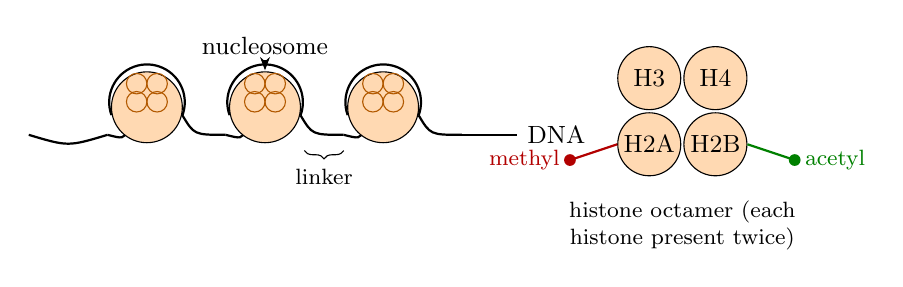
\begin{tikzpicture}[>=Stealth, every node/.style={font=\small}]
    % beads on a string
    \draw[thick] (0,0) .. controls (0.5,-0.15) .. (1,0);
    \foreach \x in {1.5,3.0,4.5} {
      \draw[thick] (\x-0.5,0) .. controls (\x-0.3,-0.05) .. (\x-0.25,0.05);
      \draw[fill=orange!30] (\x,0.35) circle (0.45);
      \foreach \dx/\dy in {-0.13/0.45,0.13/0.45,-0.13/0.22,0.13/0.22} \draw[orange!70!black] (\x+\dx,0.35+\dy-0.15) circle (0.13);
      \draw[thick] (\x-0.45,0.25) arc[start angle=200, end angle=-20, radius=0.48];
      \draw[thick] (\x+0.45,0.25) .. controls (\x+0.6,0) .. (\x+1.0,0);
    }
    \draw[thick] (5.45,0) -- (6.2,0) node[right] {DNA};
    \node[above] at (3.0,0.9) {nucleosome};
    \draw[->] (3.0,0.95) -- (3.0,0.82);
    \draw[decorate, decoration={brace, mirror, amplitude=3pt}] (3.5,-0.2) -- (4.0,-0.2) node[midway, below=3pt, font=\footnotesize] {linker};
    % histone octamer zoom
    \begin{scope}[xshift=8.3cm, yshift=0.3cm]
      \node[draw, circle, fill=orange!30, minimum size=0.8cm, inner sep=0] (h3) at (-0.42,0.42) {H3};
      \node[draw, circle, fill=orange!30, minimum size=0.8cm, inner sep=0] (h4) at (0.42,0.42) {H4};
      \node[draw, circle, fill=orange!30, minimum size=0.8cm, inner sep=0] (h2a) at (-0.42,-0.42) {H2A};
      \node[draw, circle, fill=orange!30, minimum size=0.8cm, inner sep=0] (h2b) at (0.42,-0.42) {H2B};
      \draw[red!70!black, thick] (h2a.west) -- ++(-0.6,-0.2) node[circle, fill=red!70!black, inner sep=1.5pt] {} node[left, font=\footnotesize] {methyl};
      \draw[green!50!black, thick] (h2b.east) -- ++(0.6,-0.2) node[circle, fill=green!50!black, inner sep=1.5pt] {} node[right, font=\footnotesize] {acetyl};
      \node[font=\footnotesize, align=center] at (0,-1.45) {histone octamer (each\\ histone present twice)};
    \end{scope}
  \end{tikzpicture}
  \caption{DNA wraps around nucleosomes, each an octamer of histone proteins (two each of H2A, H2B, H3 and H4), separated by linker DNA. Histone tails can carry chemical modifications such as methylation and acetylation, which are measured by ChIP-seq with modification-specific antibodies.}
  \label{fig:nucleosome}
\end{figure}

\subsection{Histone modifications}

Histones carry chemical modifications on specific amino acids, mostly on their flexible tails. Two common types are \emph{methylation}, the addition of a methyl group, and \emph{acetylation}, the addition of an acetyl group. Acetylation is generally associated with active, open chromatin, while the consequence of methylation depends on which residue is modified: some methylation marks indicate activity and others repression. The combinations of marks are sometimes called the \emph{histone code}~\citep{strahl2000,kouzarides2007}. Marks are named by the histone, the residue and the modification. For example, H3K27ac denotes acetylation (ac) of the lysine (K) at position 27 of histone H3, and H3K4me3 denotes trimethylation of lysine 4 of H3. Table~\ref{tab:histone_marks} lists the marks most often profiled, which include the core set measured by the Roadmap Epigenomics project (Section~\ref{sec:consortia}).

\begin{table}[t]
  \centering
  \caption{Commonly profiled histone modifications and the chromatin states they mark. The associations are typical rather than absolute.}
  \label{tab:histone_marks}
  \begin{tabular}{ll}
    \toprule
    Mark & Typical association \\
    \midrule
    H3K4me3 & active and poised promoters \\
    H3K4me1 & enhancers (active or primed) \\
    H3K27ac & active enhancers and promoters \\
    H3K36me3 & bodies of transcribed genes \\
    H3K27me3 & Polycomb repression, developmentally silenced genes \\
    H3K9me3 & heterochromatin, repeats \\
    \bottomrule
  \end{tabular}
\end{table}

Histone modifications are measured genome-wide with \emph{chromatin immunoprecipitation followed by sequencing} (ChIP-seq), the same assay used in Chapter 2 to measure transcription factor (TF) binding. Chromatin is crosslinked and fragmented, an antibody specific to the modified histone pulls down the fragments that carry it, and the fragments are sequenced and aligned. Regions where reads pile up carry the mark. The antibody is raised the same way as for a TF, by immunizing an animal with the modified histone. Like TF binding, histone marks differ between cell types and between healthy and diseased cells, for example in cancer.

\subsection{Chromatin accessibility}

DNA wrapped tightly around nucleosomes, or packed into dense higher-order structures, is \emph{closed} or \emph{inaccessible}: a TF cannot physically reach a binding site there, however good a match to its motif the site is. Regions with few or no nucleosomes are \emph{open} or \emph{accessible}. Active promoters and enhancers are typically accessible, because TFs and RNA polymerase II, the enzyme that transcribes genes into RNA, need to reach them. Most of the genome is closed in any given cell type; only a few percent is accessible.

\emph{ATAC-seq} (assay for transposase-accessible chromatin using sequencing) measures accessibility~\citep{buenrostro2013} (Figure~\ref{fig:atac}). The Tn5 transposase, loaded with sequencing adapters, cuts DNA and inserts the adapters at the cut site in a single step, a process called tagmentation. Tn5 can only reach naked DNA, so cuts are concentrated in open chromatin, and in the linker DNA between nucleosomes. Amplifying and sequencing the tagged fragments, and aligning the reads, gives a map of accessibility. The simplest analysis is the same as for ChIP-seq: call peaks where reads pile up. ATAC-seq works on small numbers of cells and is commercially available in a single-cell form. Its predecessor, \emph{DNase-seq}, uses the nuclease DNase I in place of Tn5 to digest accessible DNA; the accessible regions it finds are called \emph{DNase I hypersensitive sites} (DHSs)~\citep{boyle2008}. DNase-seq requires many more cells. Other assays of open chromatin, such as MNase-seq and FAIRE-seq, differ in how they fragment and enrich the DNA (Figure~\ref{fig:modalities}).

\begin{figure}[t]
  \centering
  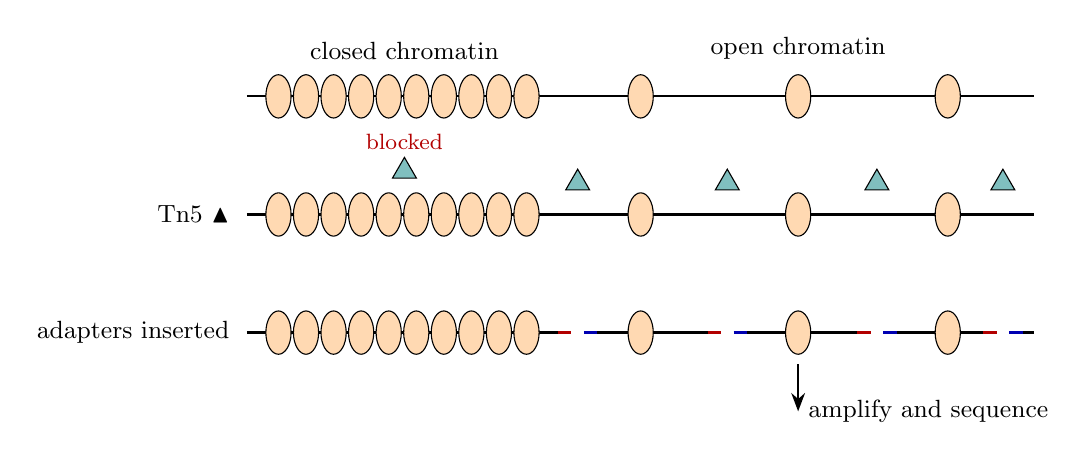
\begin{tikzpicture}[>=Stealth, every node/.style={font=\small}]
    \tikzset{nuc/.style={draw, fill=orange!30, ellipse, minimum width=0.32cm, minimum height=0.55cm, inner sep=0}}
    \tikzset{tn5/.style={draw, fill=teal!50, regular polygon, regular polygon sides=3, minimum size=0.35cm, inner sep=0}}
    \foreach \y/\lab in {0/{}, -1.5/{}, -3.0/{}} {
      \draw[thick] (0,\y) -- (10,\y);
      \foreach \x in {0.4,0.75,...,3.6} \node[nuc] at (\x,\y) {};
      \foreach \x in {5.0,7.0,8.9} \node[nuc] at (\x,\y) {};
    }
    \node[above] at (2.0,0.35) {closed chromatin};
    \node[above] at (7.0,0.35) {open chromatin};
    % Tn5
    \foreach \x in {4.2,6.1,8.0,9.6} \node[tn5] at (\x,-1.1) {};
    \node[tn5] at (2.0,-0.95) {};
    \node[above, red!70!black, font=\footnotesize] at (2.0,-0.8) {blocked};
    \node[left] at (-0.1,-1.5) {Tn5 $\blacktriangle$};
    % cut fragments
    \foreach \x in {4.2,6.1,8.0,9.6} {
      \fill[white] (\x-0.08,-3.06) rectangle (\x+0.08,-2.94);
      \draw[very thick, red!70!black] (\x-0.25,-3.0) -- (\x-0.08,-3.0);
      \draw[very thick, blue!70!black] (\x+0.08,-3.0) -- (\x+0.25,-3.0);
    }
    \node[left] at (-0.1,-3.0) {adapters inserted};
    \draw[->, thick] (7.0,-3.4) -- (7.0,-4.0) node[right] {amplify and sequence};
  \end{tikzpicture}
  \caption{ATAC-seq. The Tn5 transposase (triangles) cuts accessible DNA and inserts sequencing adapters (red and blue) in one step. Nucleosome-dense, closed chromatin is protected, as is the $\sim$147\,bp of DNA wrapped around each nucleosome. Sequencing the tagged fragments maps accessible regions. DNase-seq follows the same logic with the nuclease DNase I.}
  \label{fig:atac}
\end{figure}

\begin{figure}[t]
  \centering
  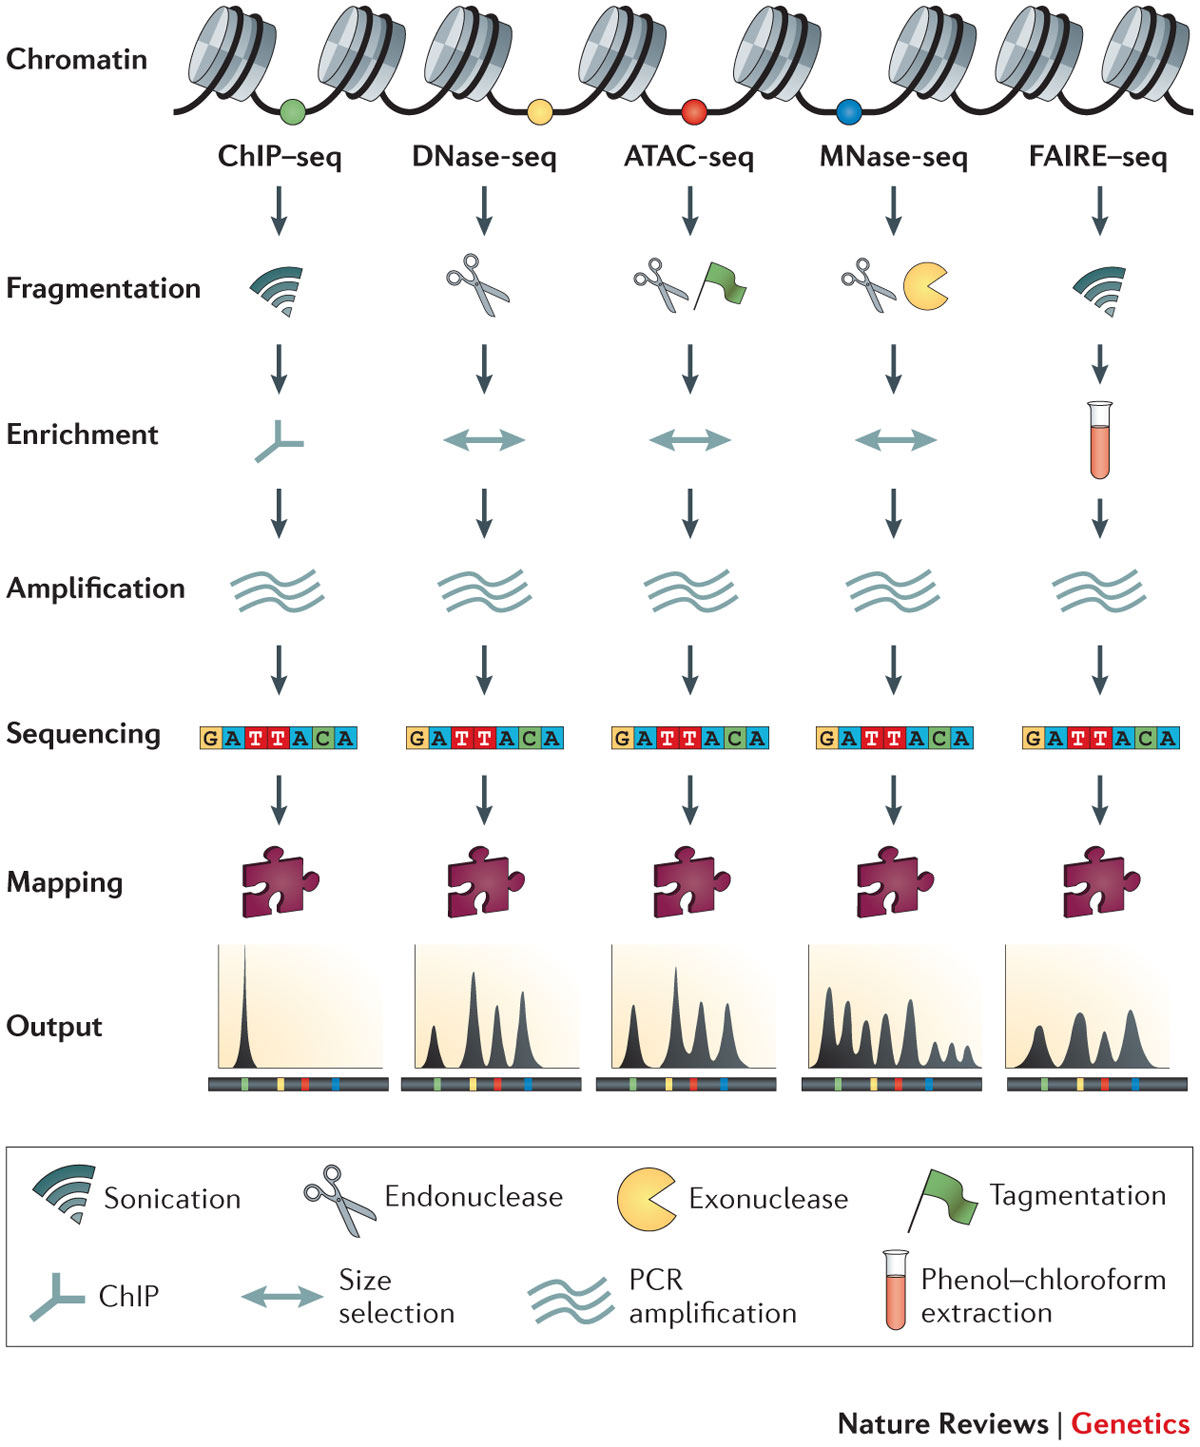
\includegraphics[width=0.55\linewidth]{slides/assay_modalities.jpg}
  \caption{Sequencing assays of chromatin: ChIP-seq, DNase-seq, ATAC-seq, MNase-seq and FAIRE-seq differ in how chromatin is fragmented and enriched before amplification, sequencing and mapping. Reproduced from \citet{meyer2014}.}
  \label{fig:modalities}
\end{figure}

The assays give complementary views of the same regulatory element (Figure~\ref{fig:assay_profiles}). Consider a TF bound in a nucleosome-depleted region flanked by nucleosomes carrying H3K27ac. ChIP-seq for the TF gives a sharp peak at the binding site. DNase-seq or ATAC-seq gives a broader peak covering the whole nucleosome-depleted region, with a dip at the binding site itself, because the bound TF protects its few base pairs of DNA from cutting. This dip is called a \emph{footprint}, and footprinting methods use it to locate bound TFs from accessibility data alone. ChIP-seq for H3K27ac gives a bimodal signal from the modified nucleosomes on either side, with little signal at the centre where there are no nucleosomes. Two further modalities, DNA methylation (methyl groups added to the DNA itself, distinct from histone methylation) and chromatin conformation measured by Hi-C, appear later in this chapter and the book.

\begin{figure}[t]
  \centering
  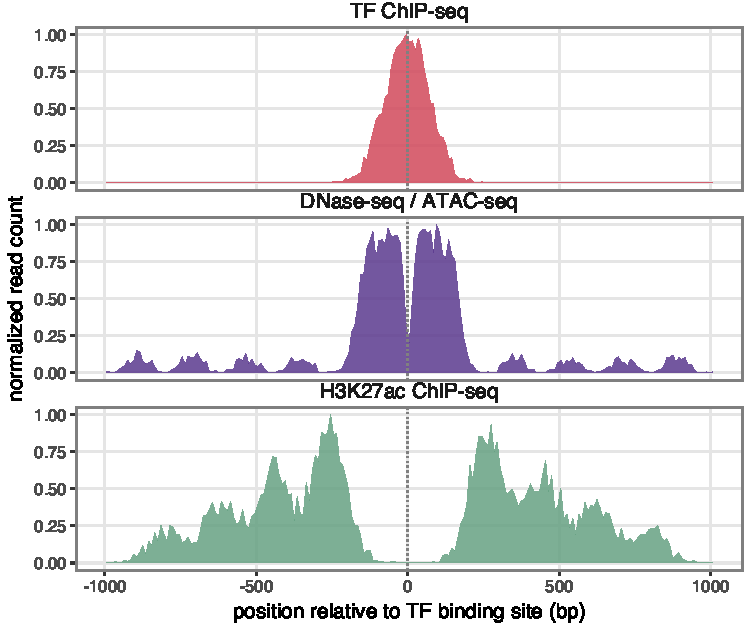
\includegraphics[width=0.7\linewidth]{assay_profiles.pdf}
  \caption{Simulated read coverage at one regulatory element, a TF bound in a nucleosome-depleted region with acetylated flanking nucleosomes. TF ChIP-seq gives a narrow peak at the binding site. Accessibility assays give a broad peak over the nucleosome-free region with a footprint (dip) where the TF protects the DNA, and weak signal in the linker DNA between nucleosomes. H3K27ac ChIP-seq gives signal on the flanking nucleosomes.}
  \label{fig:assay_profiles}
\end{figure}

%======================================================================
\section{Regulatory elements: promoters and enhancers}
\label{sec:enhancers}
%======================================================================

\emph{Regulatory elements} are stretches of DNA that are not themselves transcribed into protein-coding RNA but where TFs bind and control how much nearby genes are transcribed. The \emph{promoter} is the regulatory element immediately around a gene's transcription start site (TSS), where RNA polymerase II assembles. \emph{Enhancers} are regulatory elements further from the gene, up to around a megabase away along the linear genome. They act on their target gene through the three-dimensional folding of chromatin: a \emph{loop} brings the enhancer into physical proximity with the promoter (Figure~\ref{fig:loop}). Proteins bridge the two. The Mediator complex binds both the TFs at the enhancer and RNA polymerase II at the promoter, and the ring-shaped cohesin complex extrudes and holds loops, often anchored at sites bound by the protein CTCF.

\begin{figure}[t]
  \centering
  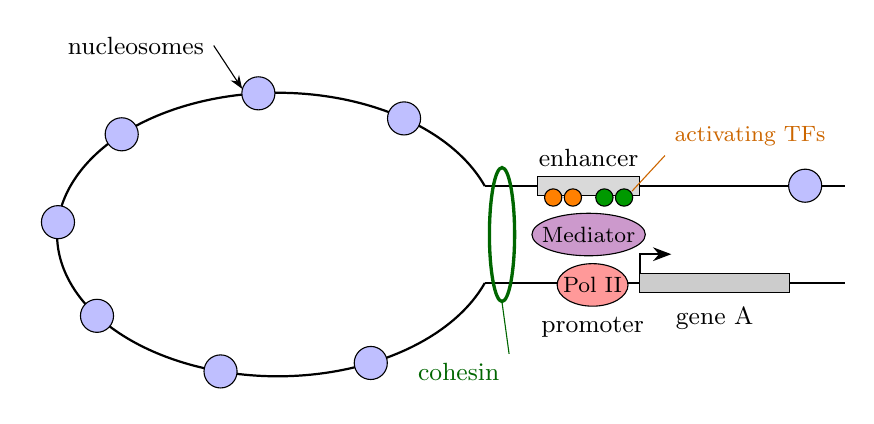
\begin{tikzpicture}[>=Stealth, every node/.style={font=\small}]
    \tikzset{nuc/.style={draw, fill=blue!25, circle, minimum size=0.42cm, inner sep=0}}
    % loop
    \draw[thick] (3,0) ++(20:2.8 and 1.8) arc[start angle=20, end angle=340, x radius=2.8, y radius=1.8];
    \foreach \a in {55,95,135,175,215,255,295} \node[nuc] at ({3+2.8*cos(\a)},{1.8*sin(\a)}) {};
    % right strands
    \draw[thick] (5.63,0.62) -- (10.2,0.62);
    \draw[thick] (5.63,-0.62) -- (10.2,-0.62);
    \node[nuc] at (9.7,0.62) {};
    % enhancer
    \draw[fill=gray!30] (6.3,0.5) rectangle (7.6,0.74);
    \node[above] at (6.95,0.74) {enhancer};
    \foreach \x/\c in {6.5/orange, 6.75/orange, 7.15/green!60!black, 7.4/green!60!black} \draw[fill=\c] (\x,0.47) circle (0.11);
    \node[font=\footnotesize, orange!80!black] (tfl) at (9.0,1.25) {activating TFs};
    \draw[orange!80!black] (tfl.south west) -- (7.5,0.55);
    % mediator
    \draw[fill=violet!40] (6.95,0.0) ellipse (0.72cm and 0.27cm);
    \node[font=\footnotesize] at (6.95,0.0) {Mediator};
    % pol II and gene
    \draw[fill=red!40] (7.0,-0.64) ellipse (0.45cm and 0.27cm);
    \node[font=\footnotesize] at (7.0,-0.64) {Pol II};
    \draw[fill=gray!40] (7.6,-0.74) rectangle (9.5,-0.5);
    \node[below] at (8.55,-0.8) {gene A};
    \draw[->, thick] (7.6,-0.5) -- (7.6,-0.25) -- (8.0,-0.25);
    \node[below] at (7.0,-0.92) {promoter};
    % cohesin
    \draw[green!40!black, very thick] (5.85,0) ellipse (0.16cm and 0.85cm);
    \node[green!40!black] (coh) at (5.3,-1.75) {cohesin};
    \draw[green!40!black] (coh.north east) -- (5.85,-0.86);
    \node (nl) at (1.2,2.4) {nucleosomes};
    \draw[->] (nl.east) -- (2.55,1.85);
  \end{tikzpicture}
  \caption{An enhancer regulates gene A through a chromatin loop that brings it close to the promoter. Activating TFs bound at the enhancer contact RNA polymerase II (Pol II) at the promoter through the Mediator complex. Cohesin holds the loop. Redrawn after a schematic used in the lecture slides.}
  \label{fig:loop}
\end{figure}

The scale of these structures differs by orders of magnitude. A nucleosome wraps about 150\,bp. Enhancer-promoter loops typically span thousands to hundreds of thousands of base pairs. A gene is usually controlled by many enhancers, often tens, and several genes and enhancers can meet at one place in the nucleus, sometimes called a transcription factory or hub. Enhancer-gene connections can also be disrupted: in some cancers, structural changes to the genome connect an enhancer to an oncogene it would not normally regulate, driving its expression.

\subsection{One genome, many cell types}

Understanding how cells with the same genome become so different is one of the central problems of biology, and the answer is written in the genome through regulatory elements. The fruit fly \textit{Drosophila melanogaster} has provided many of the clearest examples. About two to three hours after fertilization, the embryo is a single layer of around 6000 nuclei, and the pair-rule gene \textit{even-skipped} (\textit{eve}) is expressed in seven stripes along its anterior-posterior axis. The stripes foreshadow the body segments, which do not appear until hours later. Each stripe, or pair of stripes, is driven by its own enhancer; five enhancers, located upstream and downstream of the gene, produce the seven stripes.

The stripe 2 enhancer, about 500\,bp long and located roughly 1 to 1.5\,kb upstream of the TSS, is the best studied~\citep{small1992}. It contains a cluster of binding sites for both activators and repressors. The maternal activator Bicoid, whose concentration decays from the anterior end, and Hunchback, which is high in the anterior half, together switch the enhancer on across a broad anterior domain. Repressors bound to the same enhancer then cut this domain down to a stripe: Giant sets the anterior border and Kr\"uppel the posterior border. The enhancer thus integrates positive and negative inputs into a sharp on/off stripe of transcription. Figure~\ref{fig:eve} shows this logic in a toy model, where enhancer activity is a logistic function of the weighted sum of activator concentrations minus that of repressor concentrations. Separate enhancers act independently, so the full seven-stripe pattern is roughly the sum of the patterns of the individual enhancers.

\begin{figure}[t]
  \centering
  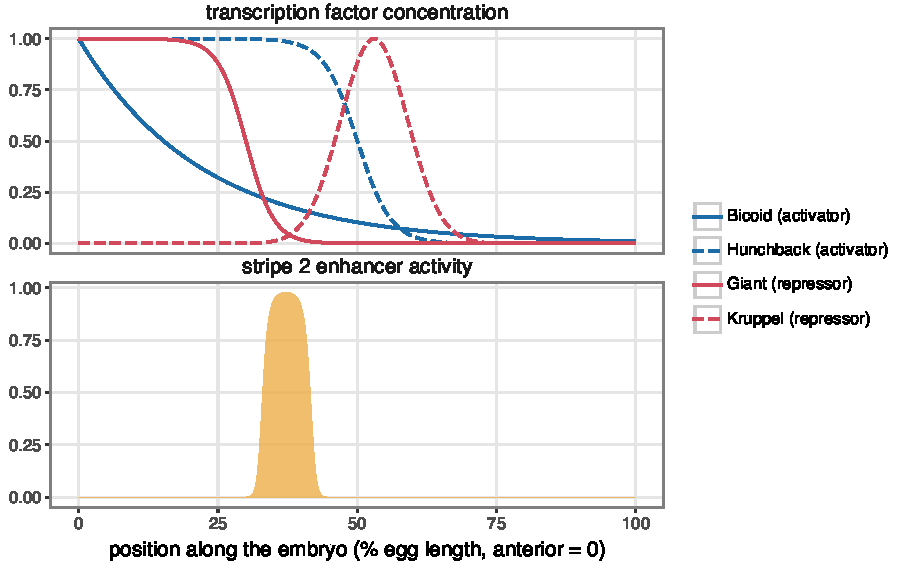
\includegraphics[width=0.85\linewidth]{eve_stripe2.pdf}
  \caption{Toy model of the \textit{eve} stripe 2 enhancer. Top: idealized concentration profiles of two activators (Bicoid, Hunchback) and two repressors (the anterior domain of Giant, simplified here to extend to the anterior tip, and Kr\"uppel) along the embryo. Bottom: enhancer activity, modelled as $\sigma(w(\text{activators}-\text{repressors})-\theta)$, is on only in a narrow stripe where activators are high and both repressors are low.}
  \label{fig:eve}
\end{figure}

The general lessons carry over to all multicellular organisms:
\begin{itemize}
  \item Enhancer-gene connectivity can change, for example during development or in disease.
  \item An enhancer usually contains binding sites for several TFs, which bind cooperatively.
  \item These TFs can be activating or repressive.
  \item TF expression, and therefore activity, varies in space and time, so the same enhancer sequence is active in some cells and not others.
\end{itemize}
The resulting picture is a regulatory network: TF levels determine which enhancers are active, enhancers determine which genes are expressed, and some of those genes are themselves TFs.

%======================================================================
\section{Mapping the regulatory genome: ENCODE and Roadmap}
\label{sec:consortia}
%======================================================================

The first draft of the human genome sequence was published in 2001, but a sequence is not an explanation: as Eric Lander put it, we had bought the book but found it hard to read. Two large consortia funded by the US National Institutes of Health set out to annotate it. The Encyclopedia of DNA Elements (ENCODE) has generated thousands of ChIP-seq experiments, for histone marks and for many TFs, together with RNA-seq, DNase-seq and, later, ATAC-seq, across many cell types~\citep{encode2012}. Most ENCODE samples are cell lines, including the cancer cell lines of Chapter 1, and a few workhorse lines such as K562 (a leukaemia line) and HepG2 (a liver cancer line) have been profiled very deeply, including with knockdown experiments that perturb individual genes. The Roadmap Epigenomics project had similar aims but focused on \emph{primary} samples, cells and tissues taken directly from donors, across essentially all organ systems and including fetal tissues~\citep{roadmap2015}. Its reference epigenomes cover more than 100 cell and tissue types, each profiled with ChIP-seq for a core set of histone marks (Table~\ref{tab:histone_marks}), DNase-seq for accessibility, whole-genome or reduced-representation bisulfite sequencing for DNA methylation, and RNA-seq for expression.

\subsection{The data as a tensor}

The data from these projects can be organized as a three-way array, or tensor (Figure~\ref{fig:tensor}). One axis is genomic position, about $3\times10^9$ base pairs, usually binned. The second is the assay, or \emph{track}: ChIP-seq for each TF and each histone mark, accessibility, methylation, RNA-seq. The third is the cell type or tissue. The tensor has hundreds of entries along each of the last two axes, and many of them are missing, in a structured way: a few cell lines have hundreds of tracks while most cell types and tissues have only a handful, often just accessibility and RNA-seq. Several computational problems arise:
\begin{itemize}
  \item \emph{Denoising}: sequencing assays are noisy, especially at low depth.
  \item \emph{Imputation}: predicting the missing (cell type, assay) combinations from the observed ones, for example by exploiting correlations between marks and between related cell types~\citep{ernst2015}.
  \item \emph{Identifying regulatory elements}: segmenting the genome into promoters, enhancers and other states in each cell type. We return to this in the chapter on hidden Markov models.
\end{itemize}

\begin{figure}[t]
  \centering
  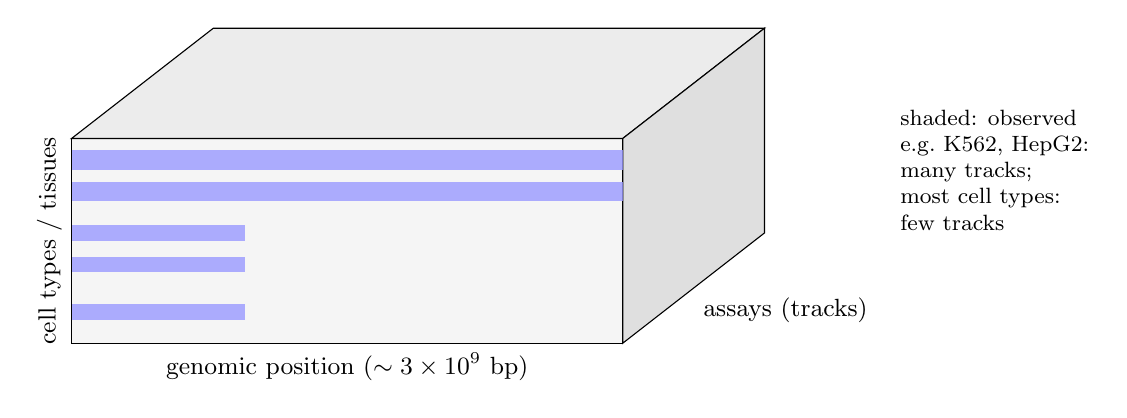
\begin{tikzpicture}[>=Stealth, every node/.style={font=\small}, x={(1cm,0cm)}, y={(0cm,1cm)}, z={(0.45cm,0.35cm)}]
    % cube: x = genome, y = cell type, z = assay
    \def\X{7} \def\Y{2.6} \def\Z{4}
    \draw[fill=gray!8] (0,0,0) -- (\X,0,0) -- (\X,\Y,0) -- (0,\Y,0) -- cycle;
    \draw[fill=gray!15] (0,\Y,0) -- (\X,\Y,0) -- (\X,\Y,\Z) -- (0,\Y,\Z) -- cycle;
    \draw[fill=gray!25] (\X,0,0) -- (\X,0,\Z) -- (\X,\Y,\Z) -- (\X,\Y,0) -- cycle;
    % observed slices (a few deeply profiled cell types)
    \foreach \y in {2.2,1.8} \fill[blue!40, opacity=0.8] (0,\y,0) -- (\X,\y,0) -- (\X,\y+0.25,0) -- (0,\y+0.25,0) -- cycle;
    \foreach \y in {0.3,0.9,1.3} \fill[blue!40, opacity=0.8] (0,\y,0) -- (2.2,\y,0) -- (2.2,\y+0.2,0) -- (0,\y+0.2,0) -- cycle;
    \node[below] at (\X/2,0,0) {genomic position ($\sim3\times10^9$ bp)};
    \node[rotate=90, above] at (0,\Y/2,0) {cell types / tissues};
    \node[anchor=north west] at (\X,0,\Z/2) {assays (tracks)};
    \node[align=left, right, font=\footnotesize] at (10.4,2.2) {shaded: observed\\ e.g.\ K562, HepG2:\\ many tracks;\\ most cell types:\\ few tracks};
  \end{tikzpicture}
  \caption{Epigenomic data as a tensor indexed by genomic position, assay and cell type. Coverage is uneven: a few cell lines are profiled with hundreds of assays, most cell types with only a few, leaving a large, structured set of missing entries to impute.}
  \label{fig:tensor}
\end{figure}

\subsection{Cell-type-specific regulatory elements}

Figure~\ref{fig:roadmap_enhancers} shows the activity of about two million enhancers (columns) across 127 reference epigenomes (rows) from Roadmap and ENCODE~\citep{roadmap2015}. The columns are clustered by their activity pattern, not ordered by genomic position, which produces a block structure. Some enhancers are active in many cell types, but most are specific to one lineage. Embryonic and induced pluripotent stem cells share a block of elements, blood cells another. Within blood, T cells have a set of elements active in all T cell samples, part of which is shared with the closely related B cells, while other elements distinguish the two. The genes near each cluster are enriched for biological processes that match the cell types in which the cluster is active, for example immune response genes near the T cell enhancers.

\begin{figure}[t]
  \centering
  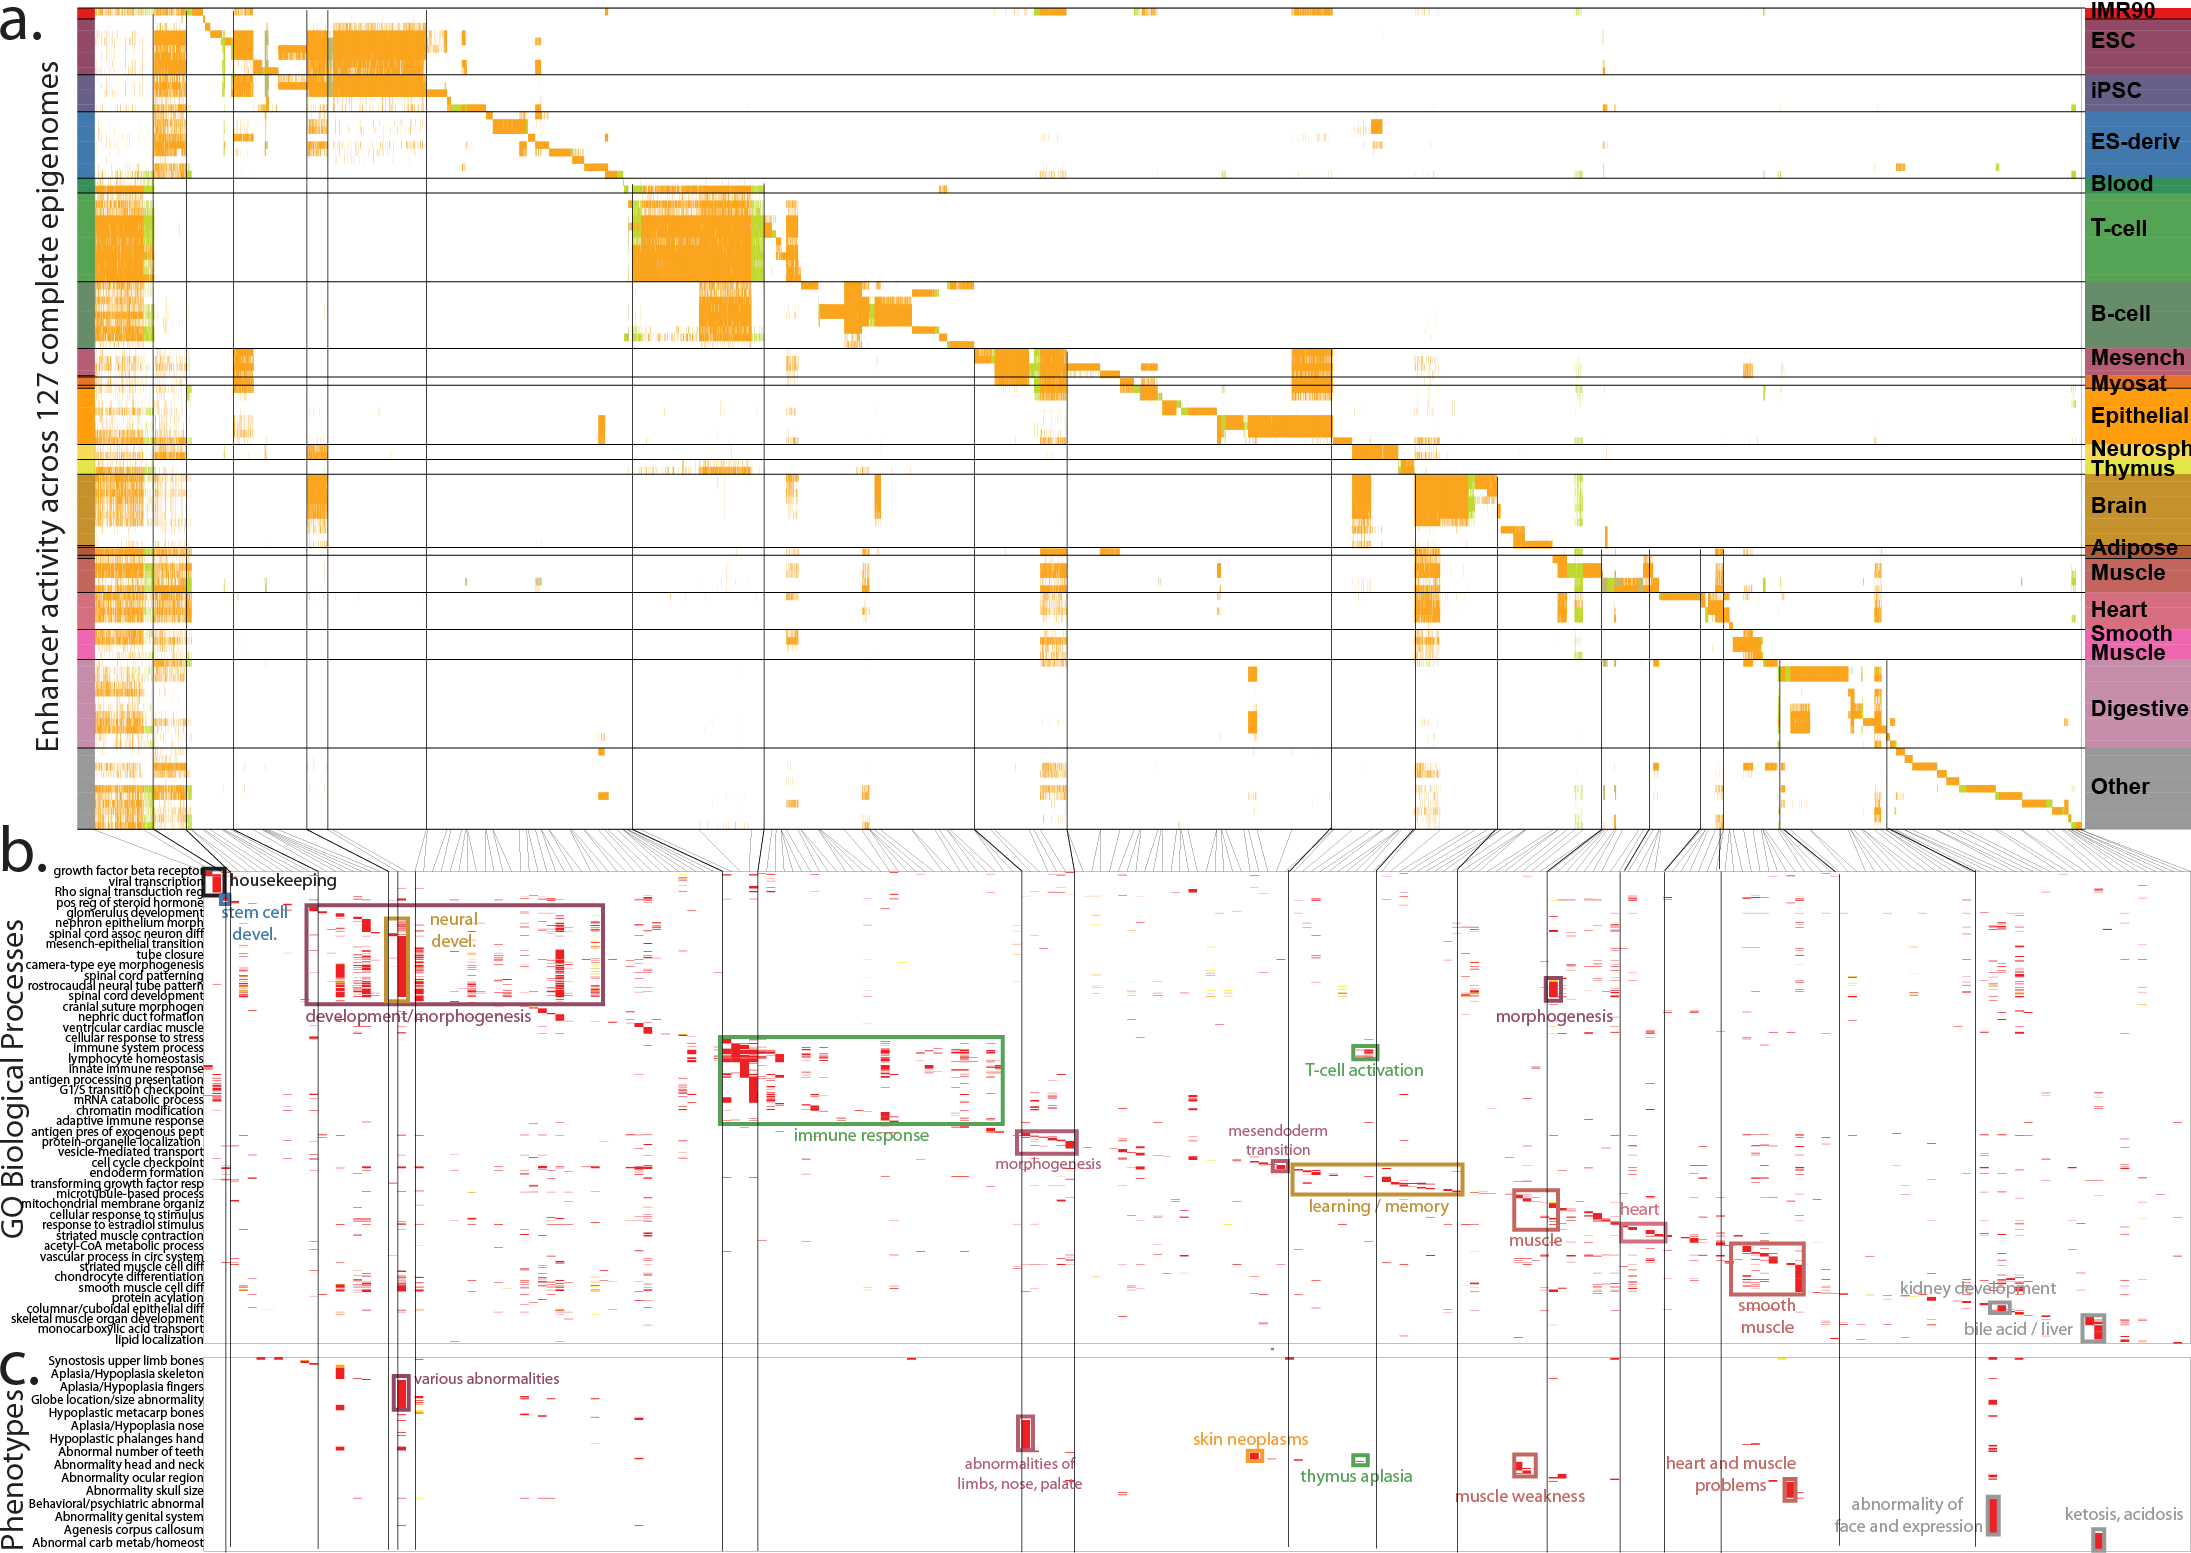
\includegraphics[width=\linewidth]{slides/roadmap_enhancer_activity.png}
  \caption{Enhancer activity across 127 reference epigenomes. (a) Rows are epigenomes grouped by tissue or cell type; columns are about two million enhancers, clustered by activity (orange, active). (b) Enrichment of Gene Ontology biological processes and (c) phenotypes among genes near each enhancer cluster. Reproduced from \citet{roadmap2015}.}
  \label{fig:roadmap_enhancers}
\end{figure}

These maps matter for human genetics. Genetic variants associated with disease in genome-wide association studies lie mostly outside protein-coding sequence, and they are enriched in regulatory elements active in cell types relevant to the disease~\citep{maurano2012}. Variants associated with autoimmune diseases, for example, are enriched in T cell and B cell enhancers. Knowing where the regulatory elements are in each cell type is a first step to explaining how a non-coding variant changes disease risk; the sequence models below are a second.

\subsection{How much of the genome is functional?}

Table~\ref{tab:functional} summarizes how much of the genome is covered by various biochemical signals when they are aggregated across hundreds of cell types~\citep{kellis2014}. Only about 1\% of the genome codes for protein. Up to a fifth is accessible or bound by some TF in some cell type, more than half carries some histone modification, and most of the genome is transcribed at some point. ENCODE's flagship paper argued that most of the genome, around 80\%, has a ``biochemical function''~\citep{encode2012}. Evolutionary biologists objected~\citep{graur2013}. Comparing the human genome with those of other mammals shows which sequences are conserved, and therefore under \emph{purifying selection}, which removes mutations that harm the organism. Without selection, sequence diverges over evolutionary time. These comparisons suggest that only 3--8\% of the genome is under selection. The two estimates use different definitions of function: biochemical activity does not imply that the activity matters for the organism. The truth is likely between them. Some functional elements are not conserved, for example because they are recent in evolution, but a histone mark or a transcript does not on its own show that a region is important.

\begin{table}[t]
  \centering
  \caption{Fraction of the human genome covered by biochemical signals, aggregated across hundreds of cell types, and the fraction estimated to be under purifying selection. Values from \citet{kellis2014}.}
  \label{tab:functional}
  \begin{tabular}{lr}
    \toprule
    Biochemical mark or element & Genomic coverage \\
    \midrule
    Protein-coding exons (GENCODE) & 1.2\% \\
    Under purifying selection & 3--8\% \\
    Regulatory elements (accessible or TF-bound) & 12--19\% \\
    Any histone modification & 56\% \\
    Transcribed in some cell type & 62\% \\
    \bottomrule
  \end{tabular}
\end{table}

%======================================================================
\section{Predicting chromatin accessibility from sequence}
\label{sec:basset}
%======================================================================

If accessibility in each cell type is determined by which TFs are present and which binding sites the sequence contains, then a model that reads DNA sequence should be able to predict accessibility. Chapter 2 developed convolutional neural networks (CNNs) for predicting TF binding from sequence; here we apply the same machinery to accessibility, across many cell types at once.

\subsection{Basset: a multitask CNN}

Basset~\citep{kelley2016} predicts DNase I hypersensitivity in 164 cell types from 600\,bp of sequence. The training examples are about two million DHSs, the union of peaks across all cell types. Let $N$ be the number of training sequences, $T=164$ the number of cell types (\emph{tasks}), and $L=600$ the sequence length. Sequence $n$ is one-hot encoded as $\mX_n\in\{0,1\}^{L\times 4}$, whose $i$-th row $\vx_{n,i}^\top$ has a single 1 in the column of the nucleotide at position $i$ (A, C, G, T). The label $y_{nt}\in\{0,1\}$ is 1 if sequence $n$ is accessible in cell type $t$. Each sequence thus has a binary vector of labels, and the matrix of labels across all sequences has the sparse, block structure of Figure~\ref{fig:roadmap_enhancers}.

The architecture is the CNN of Chapter 2 (Figure~\ref{fig:basset_arch}). The first convolutional layer has $D_1$ filters of width $k$; filter $c$ has weights $\mW_c\in\R^{k\times 4}$ and bias $b_c$, and its output at position $i$ is
\begin{equation}
  z_{i,c} = \sum_{\ell=1}^{k}\sum_{u=1}^{4} W_{c,\ell u}\,X_{n,i+\ell-1,u} + b_c ,
\end{equation}
which is the score of a position weight matrix (PWM) $\mW_c$ at position $i$, as in Chapter 2. A rectified linear unit $\max(0,z_{i,c})$ thresholds the scores, and max pooling over windows of adjacent positions reduces the length and makes the representation insensitive to the exact location of a motif. Basset stacks three convolution-ReLU-pooling blocks, with 300 filters of width 19 in the first layer, followed by two fully connected layers. The output layer has one unit per cell type, $\hat y_{nt}=\sigma(f_t(\mX_n))\in(0,1)$, where $f_t$ is the network's output for task $t$ and $\sigma$ is the logistic function. All tasks share every layer except the last, so features learned for one cell type help the others; this is \emph{multitask learning}. The loss is the binary cross-entropy of Chapter 1, summed over sequences and tasks,
\begin{equation}
  \mathcal{L} = -\sum_{n=1}^N\sum_{t=1}^T\left[y_{nt}\log\hat y_{nt} + (1-y_{nt})\log(1-\hat y_{nt})\right],
\end{equation}
and it is minimized by stochastic gradient descent with backpropagation.

\begin{figure}[t]
  \centering
  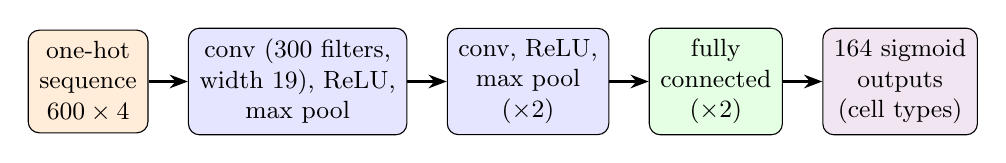
\begin{tikzpicture}[>=Stealth, every node/.style={font=\small}, box/.style={draw, rounded corners, minimum height=0.9cm, align=center, inner sep=4pt}]
    \node[box, fill=orange!15] (in) {one-hot\\sequence\\$600\times4$};
    \node[box, fill=blue!10, right=0.5cm of in] (c1) {conv (300 filters,\\ width 19), ReLU,\\ max pool};
    \node[box, fill=blue!10, right=0.5cm of c1] (c2) {conv, ReLU,\\ max pool\\ ($\times2$)};
    \node[box, fill=green!10, right=0.5cm of c2] (fc) {fully\\connected\\($\times2$)};
    \node[box, fill=violet!10, right=0.5cm of fc] (out) {164 sigmoid\\outputs\\(cell types)};
    \foreach \a/\b in {in/c1, c1/c2, c2/fc, fc/out} \draw[->, thick] (\a) -- (\b);
  \end{tikzpicture}
  \caption{The Basset architecture~\citep{kelley2016}. A one-hot encoded 600\,bp sequence passes through three convolution-ReLU-max-pooling blocks and two fully connected layers. The output layer predicts, for each of 164 cell types, the probability that the sequence is a DNase I hypersensitive site.}
  \label{fig:basset_arch}
\end{figure}

\subsection{Why a CNN beats k-mer counting}

The previous state of the art represented each sequence by its counts of \emph{k-mers}, the substrings of length $k$ (or gapped versions of them), and fitted a support vector machine (gkm-SVM)~\citep{ghandi2014}. Basset improved the area under the ROC curve (Chapter 1) in almost every cell type, from a mean of 0.780 to 0.895 (Figure~\ref{fig:basset_results}a). A k-mer representation is the sequence analogue of a bag of words in document classification: it records which words occur but not where. A CNN can model where they occur. Deeper layers can combine motif detections from the first layer, so the model can learn interactions between motifs, such as two TFs that bind cooperatively, and their \emph{grammar}: the required order, orientation and spacing of the motifs.

\begin{figure}[t]
  \centering
  \begin{subfigure}[b]{0.36\linewidth}
    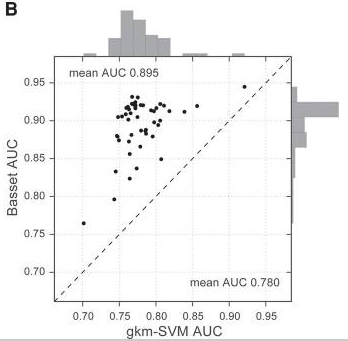
\includegraphics[width=\linewidth]{slides/basset_auc.png}
    \caption{}
  \end{subfigure}\hfill
  \begin{subfigure}[b]{0.6\linewidth}
    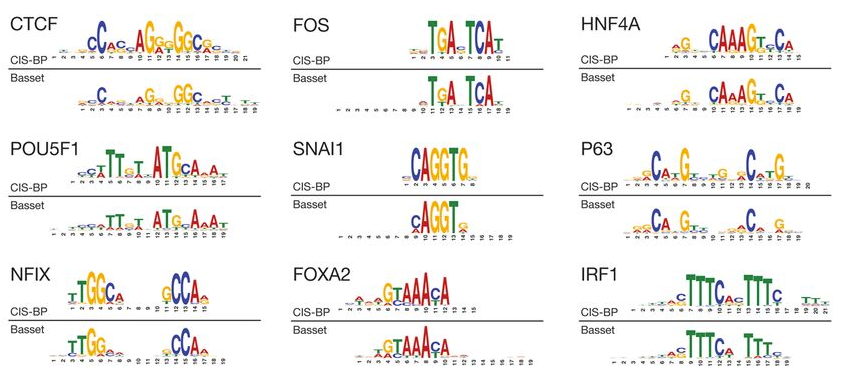
\includegraphics[width=\linewidth]{slides/basset_filters.png}
    \caption{}
  \end{subfigure}
  \caption{Basset results. (a) Area under the ROC curve per cell type for Basset against the gapped k-mer SVM (gkm-SVM). (b) First-layer filters, displayed as sequence logos, beside the best-matching known TF motif from the CIS-BP database. Reproduced from \citet{kelley2016}.}
  \label{fig:basset_results}
\end{figure}

\subsection{First-layer filters are motifs}

Because a first-layer filter computes a PWM score at every position, each filter can be visualized as a motif. Basset did so by collecting the sequence windows that activate a filter most strongly and summarizing them as a position frequency matrix. About 45\% of the 300 first-layer filters matched a known TF motif in the CIS-BP database~\citep{weirauch2014}, including CTCF, the AP-1 factor FOS, HNF4A and FOXA2 (Figure~\ref{fig:basset_results}b). The model learned these motifs from accessibility data alone, without being given any known motifs. The unmatched filters may be redundant or unused, may capture partial motifs that deeper layers assemble, or may correspond to TFs whose motifs are not in the database. Not every architecture learns such readable first-layer filters; Chapter 4 discusses this and other interpretation methods.

\subsection{In silico mutagenesis and genetic variants}
\label{sec:ism}

A trained model can predict the effect of changing the sequence. A \emph{genetic variant} is an inherited difference between individuals; the most common type is a \emph{single nucleotide polymorphism} (SNP), a single position at which people carry different nucleotides (\emph{alleles}). SNPs have identifiers of the form rs followed by a number, which index the dbSNP database. A \emph{mutation}, by contrast, is a new change, such as a somatic mutation in a tumour. To predict a variant's effect, we compare the model's predictions for the sequences carrying each allele.

\emph{In silico mutagenesis} (ISM) does this systematically. For a sequence $\mX$ and output $f$ (for example the predicted accessibility logit in one cell type), let $\mX^{(i\to u)}$ be the sequence with position $i$ changed to nucleotide $u$. The ISM score is
\begin{equation}
  \Delta_{iu} = f\big(\mX^{(i\to u)}\big) - f(\mX), \qquad i=1,\dots,L,\quad u\in\{\text{A},\text{C},\text{G},\text{T}\},
\end{equation}
an $L\times4$ matrix that is zero at the reference nucleotides. Computing it costs $3L$ forward passes. Figure~\ref{fig:basset_ism} shows ISM around the SNP rs4409785, which is associated with vitiligo, rheumatoid arthritis and multiple sclerosis~\citep{kelley2016}. With the reference allele T, almost no single change matters. Changing the T to the alternative allele C sharply increases predicted accessibility, because it completes a strong match to the CTCF motif. ISM on the sequence carrying the C allele then shows that the surrounding nucleotides matter too: mutating the rest of the CTCF motif abolishes the predicted gain. Such analyses suggest which TF a variant affects, which can then be checked against databases of known motifs and tested experimentally. We return to methods for explaining model predictions, of which ISM is the simplest, in Chapter 4.

\begin{figure}[t]
  \centering
  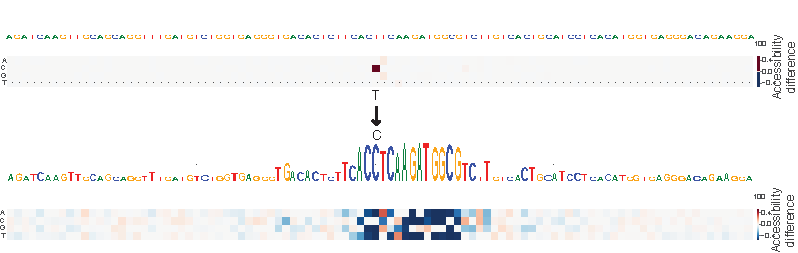
\includegraphics[width=0.9\linewidth]{slides/basset_ism.pdf}
  \caption{In silico mutagenesis around SNP rs4409785. Top: the reference sequence and the predicted change in accessibility for each possible single-nucleotide change (rows A, C, G, T); only the T$\to$C change at the SNP has a large effect. Bottom: with the C allele, the sequence logo (letter heights proportional to the effect of mutating that position) and heatmap reveal a CTCF motif around the variant. Reproduced from \citet{kelley2016}.}
  \label{fig:basset_ism}
\end{figure}

%======================================================================
\section{The limited reach of convolutions}
\label{sec:receptive}
%======================================================================

The \emph{receptive field} of a unit in a CNN is the set of input positions that can affect it. A convolution of width $k$ is local: a unit in the first layer sees $k$ positions, and each further layer of width-$k$ convolutions extends the receptive field by $k-1$ positions of the layer below (Figure~\ref{fig:cnn_attention}a). Let $r_d$ be the receptive field after $d$ layers, measured in input positions, and $\delta_d$ the spacing, in input positions, between adjacent units of layer $d$ (the product of the strides and pooling sizes up to layer $d$, with $\delta_0=1$ and $r_0=1$). Then
\begin{equation}
  r_d = r_{d-1} + (k-1)\,\delta_{d-1}.
\end{equation}
For stride-one convolutions without pooling, $\delta_d=1$ and $r_d=1+d(k-1)$, which grows linearly with depth: doubling the context means doubling the number of layers. Max pooling with window and stride 2 after each layer doubles $\delta$ at each layer, so the receptive field grows exponentially, at the price of halving the resolution each time. \emph{Dilated} convolutions~\citep{yu2016}, used in Basenji~\citep{kelley2018}, skip input positions: a width-$k$ filter with dilation $2^{d-1}$ at layer $d$ applies its weights to positions $2^{d-1}$ apart, so $r_d=1+(k-1)(2^d-1)$, also exponential, without losing resolution (Figure~\ref{fig:receptive_field}).

\begin{figure}[t]
  \centering
  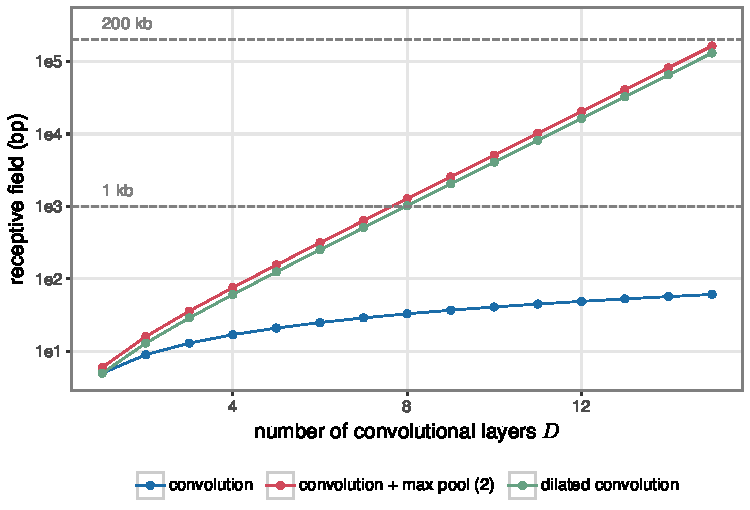
\includegraphics[width=0.65\linewidth]{receptive_field.pdf}
  \caption{Receptive field against depth for width-5 convolutions: stride-one convolutions (linear growth), convolutions each followed by max pooling of width 2, and dilated convolutions with dilation doubling at each layer (both exponential). Enhancers act on genes over distances of $10^4$ to $10^5$\,bp or more.}
  \label{fig:receptive_field}
\end{figure}

This matters because enhancers can act on genes tens or hundreds of kilobases away. In the language analogy, predicting the next word well needs the whole paragraph or chapter, not just the current sentence. Even with an exponentially growing receptive field, information from distant positions has to pass through many layers before it can interact, and the convolution weights treat each relative offset in the same fixed way regardless of what the sequence contains. Attention removes both restrictions.

\begin{figure}[t]
  \centering
  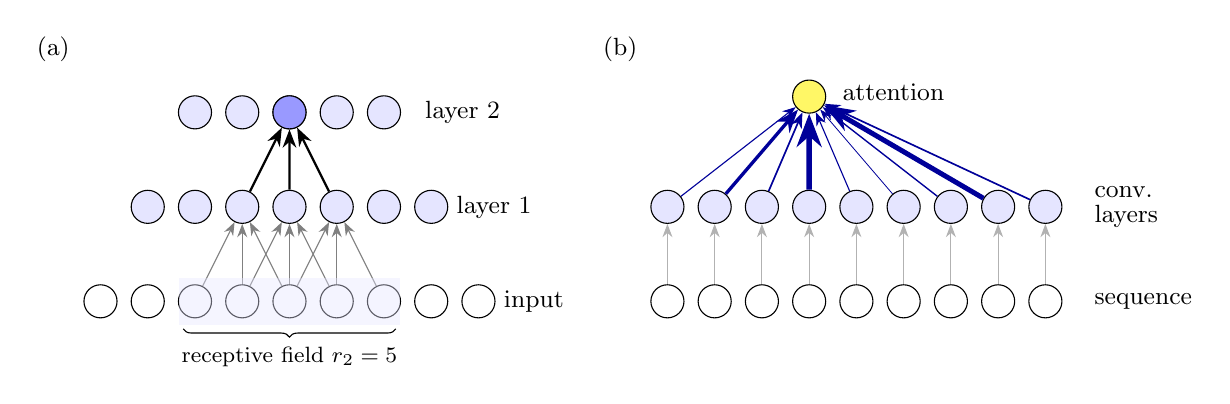
\begin{tikzpicture}[>=Stealth, every node/.style={font=\small}]
    \tikzset{u/.style={draw, circle, minimum size=0.42cm, inner sep=0, fill=blue!10}}
    % (a) CNN
    \node at (-0.6,3.2) {(a)};
    \foreach \x in {0,...,8} \node[u, fill=white] (a0\x) at (0.6*\x,0) {};
    \foreach \x in {1,...,7} \node[u] (a1\x) at (0.6*\x,1.2) {};
    \foreach \x in {2,...,6} \node[u] (a2\x) at (0.6*\x,2.4) {};
    \node[u, fill=blue!40] (top) at (2.4,2.4) {};
    \foreach \x in {3,4,5} \draw[->, thick] (a1\x) -- (top);
    \foreach \x/\y in {2/3,3/3,4/3,3/4,4/4,5/4,4/5,5/5,6/5} \draw[->, gray] (a0\x) -- (a1\y);
    \fill[blue!10, opacity=0.4] (1.0,-0.3) rectangle (3.8,0.3);
    \node[right] at (5.0,0) {input};
    \node[right] at (4.4,1.2) {layer 1};
    \node[right] at (4.0,2.4) {layer 2};
    \draw[decorate, decoration={brace, mirror, amplitude=3pt}] (1.05,-0.35) -- (3.75,-0.35) node[midway, below=3pt, font=\footnotesize] {receptive field $r_2=5$};
    % (b) conv + attention
    \begin{scope}[xshift=7.2cm]
      \node at (-0.6,3.2) {(b)};
      \foreach \x in {0,...,8} \node[u, fill=white] (b0\x) at (0.6*\x,0) {};
      \foreach \x in {0,...,8} \node[u] (b1\x) at (0.6*\x,1.2) {};
      \foreach \x in {0,...,8} \draw[->, gray!60] (b0\x) -- (b1\x);
      \node[u, fill=yellow!60] (q) at (1.8,2.6) {};
      \foreach \x/\w in {0/0.4, 1/1.2, 2/0.6, 3/2.0, 4/0.4, 5/0.3, 6/0.5, 7/1.8, 8/0.6} \draw[->, line width=\w pt, blue!60!black] (b1\x) -- (q);
      \node[right] at (5.3,0) {sequence};
      \node[right, align=left] at (5.3,1.2) {conv.\\[-2pt] layers};
      \node[right] at (2.1,2.65) {attention};
    \end{scope}
  \end{tikzpicture}
  \caption{(a) In a CNN with width-3 convolutions, a unit in layer 2 depends on five input positions; its receptive field grows by two positions per layer. (b) In a hybrid model, convolutional layers extract local features and an attention layer lets each position draw on every position in the sequence. Edge widths illustrate the attention weights of one position (yellow), which can be large for distant positions.}
  \label{fig:cnn_attention}
\end{figure}

%======================================================================
\section{Attention and transformers}
\label{sec:attention}
%======================================================================

Transformers~\citep{vaswani2017} are the architecture behind modern large language models: the T in GPT stands for transformer. Their central component is \emph{attention}, a layer in which every position in a sequence can take information from every other position, with weights that depend on the input itself. Figure~\ref{fig:attention_matrices} contrasts the two. A width-3 convolution, viewed as a matrix whose entry $(i,j)$ says how much output position $i$ uses input position $j$, is banded: each row draws only on three neighbouring positions, and the pattern is the same for every input. An attention matrix is dense, and it is recomputed for each input sequence. This section derives the attention layer, following the standard formulation (see also Section 15.4 of \citealp{murphy2022}).

\begin{figure}[t]
  \centering
  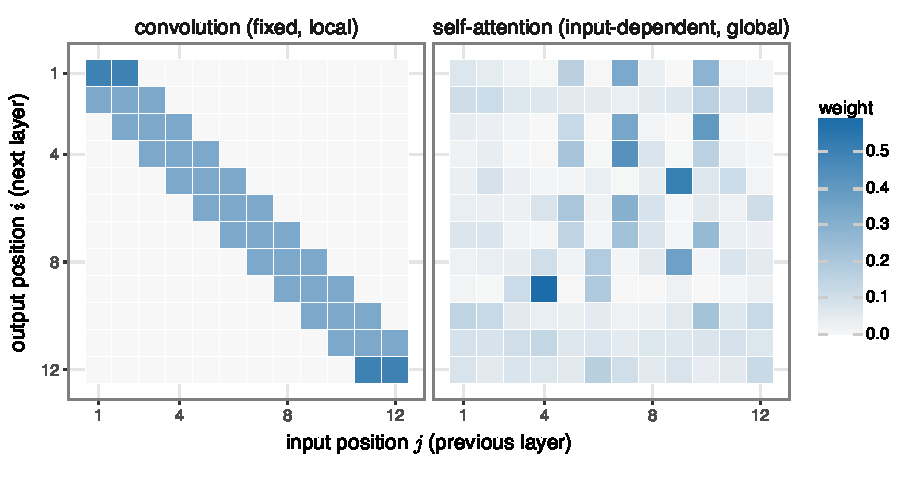
\includegraphics[width=0.85\linewidth]{attention_matrices.pdf}
  \caption{Which positions of the previous layer each position of the next layer draws on. Left: a width-3 convolution, with uniform weights for display, is a fixed banded pattern. Right: a self-attention matrix $\mA$ computed from a random input and random projections; each row is a probability vector over all $L=12$ positions and changes with the input.}
  \label{fig:attention_matrices}
\end{figure}

\subsection{Self-attention}

Let $L$ be the sequence length and $D$ the number of channels. The input to an attention layer is a matrix $\mH\in\R^{L\times D}$ whose $i$-th row $\vh_i^\top$ is the representation of position $i$; in a genomic model $\vh_i$ might be the output of convolutional layers at position $i$. We want, for each pair of positions $(i,j)$, a weight $a_{ij}\geq0$ that says how much position $i$ attends to, or takes information from, position $j$. The weight should depend on both $\vh_i$ and $\vh_j$, and the weights for each $i$ should sum to one over $j$, so that each position has a fixed budget of attention to spend across the sequence.

From each position we compute three vectors by linear maps (Figure~\ref{fig:attention_diagram}),
\begin{equation}
  \underbrace{\vq_i}_{P\times1} = \underbrace{\mW^Q}_{P\times D}\underbrace{\vh_i}_{D\times1}, \qquad
  \vk_j = \mW^K\vh_j \in\R^P, \qquad
  \vv_j = \mW^V\vh_j \in\R^{D_v},
\end{equation}
called the \emph{query}, \emph{key} and \emph{value}. The parameters of the layer are the matrices $\mW^Q,\mW^K\in\R^{P\times D}$ and $\mW^V\in\R^{D_v\times D}$; $\mW^Q$ and $\mW^K$ have the same shape but are different matrices. The query and key dimension $P$ and the value dimension $D_v$ are hyperparameters, often both equal to $D$. Position $i$ should attend to position $j$ when its query matches the key of $j$, measured by the scaled inner product
\begin{equation}
  s_{ij} = \frac{\vq_i^\top\vk_j}{\sqrt{P}} .
\end{equation}
The scores $s_{ij}$ can be positive or negative and do not sum to one, so we normalize each row with the softmax function of Chapter 1,
\begin{equation}
  a_{ij} = \softmax_j(\vs_{i})_j = \frac{\exp(s_{ij})}{\sum_{j'=1}^L\exp(s_{ij'})},
  \label{eq:attn_softmax}
\end{equation}
where $\vs_i\in\R^L$ is the vector of scores of query $i$ against all keys. The output at position $i$ is the attention-weighted average of the values,
\begin{equation}
  \underbrace{\vg_i}_{D_v\times1} = \sum_{j=1}^{L} \underbrace{a_{ij}}_{1\times1}\,\underbrace{\vv_j}_{D_v\times1} .
  \label{eq:attn_output}
\end{equation}
The sum includes $j=i$, so a position can keep its own information. In the next layer, $\vg_i$ replaces $\vh_i$. Because queries, keys and values are all computed from the same sequence, this is called \emph{self-attention}.

\begin{figure}[t]
  \centering
  \begin{tikzpicture}[>=Stealth, every node/.style={font=\small}]
    \tikzset{vec/.style={draw, minimum width=0.35cm, minimum height=1.0cm, inner sep=0}}
    \node[vec, fill=gray!15, label=above:$\vh_1$] (h1) at (0,0) {};
    \node[vec, fill=gray!15, label=above:$\vh_2$] (h2) at (4.5,0) {};
    \node at (6.5,0) {$\cdots$};
    \node[vec, fill=gray!15, label=above:$\vh_L$] (hL) at (8,0) {};
    \node (q1) at (-1.0,-1.8) {$\vq_1$}; \node (k1) at (0,-1.8) {$\vk_1$}; \node (v1) at (1.0,-1.8) {$\vv_1$};
    \node (q2) at (3.5,-1.8) {$\vq_2$}; \node (k2) at (4.5,-1.8) {$\vk_2$}; \node (v2) at (5.5,-1.8) {$\vv_2$};
    \draw[->] (h1) -- (q1); \draw[->] (h1) -- (k1); \draw[->] (h1) -- (v1);
    \node[font=\footnotesize, align=left] at (2.3,-0.9) {$\vq_i=\mW^Q\vh_i$\\ $\vk_i=\mW^K\vh_i$\\ $\vv_i=\mW^V\vh_i$};
    \draw[->] (h2) -- (q2); \draw[->] (h2) -- (k2); \draw[->] (h2) -- (v2);
    \node (s12) at (1.8,-3.2) {$s_{12}=\vq_1^\top\vk_2/\sqrt{P}$};
    \draw[->] (q1) -- (s12); \draw[->] (k2) -- (s12);
    \node (a12) at (1.8,-4.3) {$a_{12}=\softmax_j(\vs_1)_2$};
    \draw[->] (s12) -- (a12);
    \node (g1) at (4.6,-5.4) {$\vg_1=\sum_j a_{1j}\vv_j$};
    \draw[->] (a12) -- (g1);
    \draw[->] (v2) to[out=-80, in=60] (g1);
    \draw[decorate, decoration={brace, amplitude=3pt}] (-0.25,0.5) -- (-0.25,-0.5) ;
    \node[left] at (-0.35,0) {$D$ channels};
  \end{tikzpicture}
  \caption{Computing one term of self-attention. Each position's representation $\vh_i$ is mapped to a query, a key and a value. The inner product of the query of position 1 and the key of position 2, normalized over all keys by the softmax, gives the weight $a_{12}$ with which position 1 takes the value of position 2. The output $\vg_1$ sums such contributions over all positions.}
  \label{fig:attention_diagram}
\end{figure}

\paragraph{Matrix form.} Stacking the vectors as rows, $\mQ=\mH\mW^{Q\top}\in\R^{L\times P}$, $\mK=\mH\mW^{K\top}\in\R^{L\times P}$ and $\mV=\mH\mW^{V\top}\in\R^{L\times D_v}$. The score matrix is $\mS=\mQ\mK^\top/\sqrt{P}$, with dimensions $[L\times P][P\times L]=[L\times L]$, the attention matrix is $\mA=\softmax(\mS)$ with the softmax applied to each row, and the output is
\begin{equation}
  \underbrace{\mG}_{L\times D_v} = \underbrace{\mA}_{L\times L}\,\underbrace{\mV}_{L\times D_v} = \softmax\!\left(\frac{\mQ\mK^\top}{\sqrt{P}}\right)\mV .
  \label{eq:attention_matrix}
\end{equation}
Written this way the layer is a few matrix products, which GPUs compute efficiently.

\paragraph{Why divide by $\sqrt{P}$?} Suppose the entries of $\vq_i$ and $\vk_j$ are independent with mean zero and variance one, as they roughly are at initialization with suitably scaled weights. Then $\E[\vq_i^\top\vk_j]=0$ and
\begin{equation}
  \operatorname{Var}\left(\vq_i^\top\vk_j\right) = \sum_{p=1}^P\operatorname{Var}(q_{ip}k_{jp}) = \sum_{p=1}^P\E[q_{ip}^2]\,\E[k_{jp}^2] = P ,
\end{equation}
so the raw inner products have standard deviation $\sqrt{P}$, and dividing by $\sqrt{P}$ gives scores of unit variance whatever $P$ is. Without the scaling, large $P$ produces large score differences, and the softmax \emph{saturates}: nearly all the weight goes to one position (Figure~\ref{fig:attention_scaling}). Saturation stalls learning, because the derivative of the softmax, $\partial a_{ij}/\partial s_{ij'} = a_{ij}(\ind[j=j']-a_{ij'})$, is close to zero for every $j,j'$ when one $a_{ij}$ is close to one and the rest close to zero.

\begin{figure}[t]
  \centering
  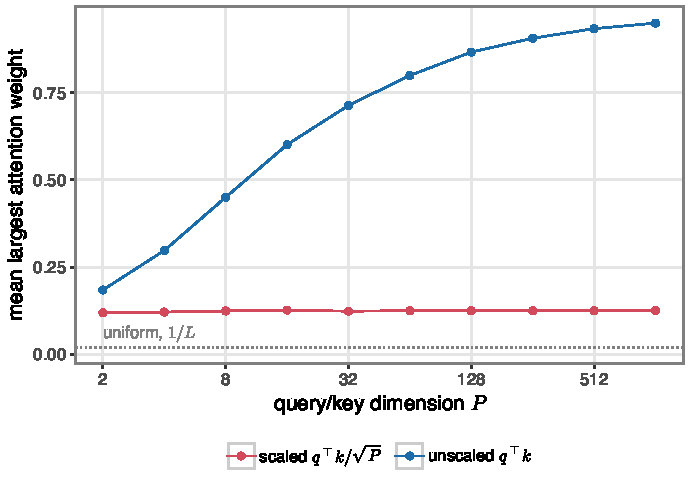
\includegraphics[width=0.6\linewidth]{attention_scaling.pdf}
  \caption{Mean largest attention weight for one query against $L=50$ keys with independent standard normal entries, as a function of the dimension $P$ (2000 replicates). Without scaling the softmax saturates toward a single position as $P$ grows; with the $1/\sqrt{P}$ scaling the attention distribution is unchanged.}
  \label{fig:attention_scaling}
\end{figure}

\paragraph{Attention as a learned graph.} The matrix $\mA$ can be read as the weighted adjacency matrix of a directed graph on the $L$ positions, with $a_{ij}$ the amount of information passed from node $j$ to node $i$. Every node passes information to every other node at once. Graph neural networks also pass messages along the edges of a graph, but there the graph, for example the bonds of a molecule, is given as input. Attention constructs the graph from the data, separately for each input. The graph is not symmetric in general: $s_{ij}\neq s_{ji}$ because the query and key maps differ. If we tied them, $\mW^Q=\mW^K$, the scores would be symmetric, and positions would attend to positions with similar representations. With separate maps the model can learn to attend to positions that are similar or dissimilar in whatever sense is useful for the prediction.

\paragraph{Comparison with convolution.} A stride-one convolution of width $k$ with input and output channels $D$ computes $\vg_i=\sum_{\ell=-(k-1)/2}^{(k-1)/2}\mW_\ell\vh_{i+\ell}$, with a separate $D\times D$ weight matrix $\mW_\ell$ for each offset $\ell$ and odd $k$. Self-attention computes $\vg_i=\sum_{j=1}^L a_{ij}\mW^V\vh_j$: one weight matrix shared by all positions, multiplied by a scalar weight $a_{ij}$ that depends on the content of positions $i$ and $j$ rather than only their offset. The convolution is local and fixed after training; attention is global and input-dependent.

\subsection{The transformer block}

An attention layer is combined with a position-wise multilayer perceptron (MLP) into a \emph{transformer block}. In the variant used by most current models, each sub-layer is preceded by layer normalization (LN)~\citep{ba2016}, which rescales each position's vector to zero mean and unit variance across channels followed by a learned scale and shift, and wrapped in a residual connection~\citep{he2016},
\begin{align}
  \mH' &= \mH + \operatorname{MHA}\big(\operatorname{LN}(\mH)\big), \\
  \mH^{\text{out}} &= \mH' + \operatorname{MLP}\big(\operatorname{LN}(\mH')\big),
\end{align}
where MHA is multi-head attention (below) and the MLP, applied to each position separately, is $\operatorname{MLP}(\vh)=\mW_2\max(0,\mW_1\vh+\mathbf{c}_1)+\mathbf{c}_2$ with $\mW_1\in\R^{D_{\text{ff}}\times D}$, $\mW_2\in\R^{D\times D_{\text{ff}}}$ and biases $\mathbf{c}_1\in\R^{D_{\text{ff}}}$, $\mathbf{c}_2\in\R^{D}$. The residual connections let each block learn a correction to its input and keep gradients flowing through deep stacks. Attention mixes information across positions; the MLP transforms the features at each position. A transformer stacks many such blocks. All weight matrices are initialized randomly and learned jointly by backpropagation of a single loss at the output, whether that is predicting the next word or the accessibility of a sequence.

\subsection{Multi-head attention}

A single attention matrix expresses one pattern of which positions are relevant to which. In practice several attention computations, called \emph{heads}, are run in parallel (Figure~\ref{fig:multihead}). Head $m=1,\dots,M$ has its own projections $\mW^Q_m,\mW^K_m\in\R^{P\times D}$ and $\mW^V_m\in\R^{(D/M)\times D}$ and computes $\mG_m=\softmax(\mQ_m\mK_m^\top/\sqrt{P})\mV_m\in\R^{L\times D/M}$ as in~\eqref{eq:attention_matrix}. The head outputs are concatenated along the channel dimension and mixed by an output projection $\mW^O\in\R^{D\times D}$,
\begin{equation}
  \operatorname{MHA}(\mH) = \big[\mG_1,\dots,\mG_M\big]\,\mW^{O\top} \in\R^{L\times D} .
\end{equation}
Dividing the value dimension by $M$ keeps the number of output channels, and the cost, the same as for a single head of full width. Concatenating along the sequence dimension instead would change the number of positions, which is not what we want. Using several heads is not the same as using one head with larger $P$: however large $P$ is, a single head produces one attention matrix, whereas $M$ heads produce $M$ different matrices. Each head can learn a different notion of relevance. In language, a noun might attend to its adjectives in one head and to the subject of the sentence in another. In regulatory sequence, some cofactors bind close to a TF and others further away, and different heads could capture these different ranges. Typical models use from 4 to 16 heads.

\begin{figure}[t]
  \centering
  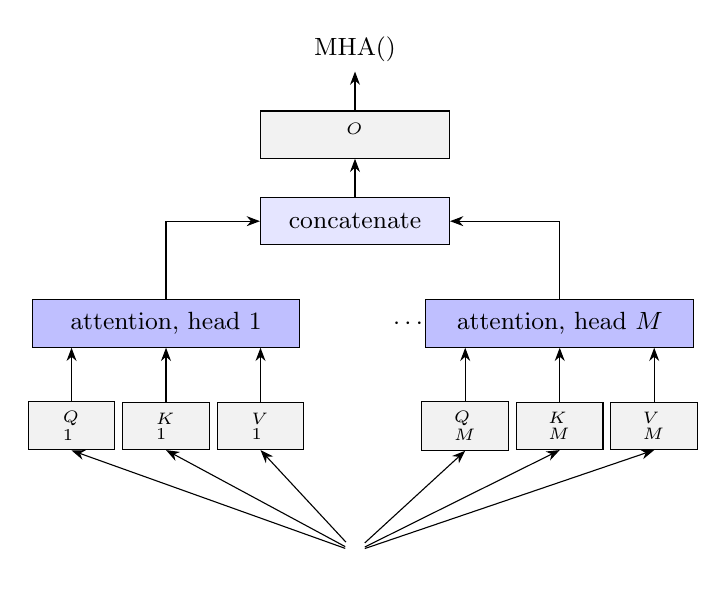
\begin{tikzpicture}[>=Stealth, every node/.style={font=\small}, b/.style={draw, minimum height=0.6cm, minimum width=1.1cm, align=center}]
    \node (Hin) at (3.6,-1.6) {$\mH$};
    \foreach \m/\x in {1/0, M/5.0} {
      \node[b, fill=gray!10] (q\m) at (\x,0) {$\mW^Q_{\m}$};
      \node[b, fill=gray!10] (k\m) at (\x+1.2,0) {$\mW^K_{\m}$};
      \node[b, fill=gray!10] (v\m) at (\x+2.4,0) {$\mW^V_{\m}$};
      \node[b, fill=blue!25, minimum width=3.4cm] (att\m) at (\x+1.2,1.3) {attention, head $\m$};
      \foreach \w in {q,k,v} {\draw[->] (\w\m) -- (\w\m |- att\m.south); \draw[->] (Hin) -- (\w\m.south);}
    }
    \node at (4.3,1.3) {$\cdots$};
    \node[b, fill=blue!10, minimum width=2.4cm] (cat) at (3.6,2.6) {concatenate};
    \node[b, fill=gray!10, minimum width=2.4cm] (out) at (3.6,3.7) {$\mW^O$};
    \draw[->] (att1) |- (cat); \draw[->] (attM) |- (cat);
    \draw[->] (cat) -- (out);
    \draw[->] (out) -- ++(0,0.8) node[above] {$\operatorname{MHA}(\mH)$};
  \end{tikzpicture}
  \caption{Multi-head attention. Each head projects the input to its own queries, keys and values and computes its own attention; the head outputs are concatenated along the channel dimension and mixed by the output projection $\mW^O$.}
  \label{fig:multihead}
\end{figure}

\subsection{Cost and path length}

Table~\ref{tab:complexity} compares the per-layer cost of attention with that of convolutional and recurrent layers~\citep{vaswani2017}, for sequence length $L$, $D$ channels and convolution width $k$. Computing $\mS$ requires $L^2$ inner products of length $P\approx D$, so attention costs $O(L^2D)$ per layer, quadratic in the sequence length. This is its main drawback, and much engineering, and many alternative architectures, aim to reduce it. Its advantage is the \emph{maximum path length}, the number of layers information must traverse to travel between the two ends of the sequence: one, for attention. For stride-one convolutions the receptive field grows by $k-1$ per layer, so connecting positions $L$ apart takes $(L-1)/(k-1)=O(L/k)$ layers, or $O(\log_k L)$ with dilated convolutions. Recurrent neural networks, covered in a later chapter, pass information along the sequence one position at a time. Their path length is $O(L)$ and they need $O(L)$ sequential operations per layer, a for loop that cannot exploit the parallelism of GPUs, whereas convolutions and attention compute all positions at once.

\begin{table}[t]
  \centering
  \caption{Per-layer cost, number of sequential operations and maximum path length between any two positions, for sequence length $L$, $D$ channels and convolution width $k$. Adapted from \citet{vaswani2017}.}
  \label{tab:complexity}
  \begin{tabular}{llll}
    \toprule
    Layer type & Cost per layer & Sequential operations & Maximum path length \\
    \midrule
    Self-attention & $O(L^2D)$ & $O(1)$ & $O(1)$ \\
    Recurrent & $O(LD^2)$ & $O(L)$ & $O(L)$ \\
    Convolutional & $O(kLD^2)$ & $O(1)$ & $O(L/k)$; $O(\log_k L)$ if dilated \\
    \bottomrule
  \end{tabular}
\end{table}

In genomics, transformers are rarely applied directly to nucleotides. State-of-the-art models first apply convolutional layers, which extract local features such as motifs and, through pooling, shorten the sequence, and then apply transformer blocks to the shorter sequence of feature vectors (Figure~\ref{fig:cnn_attention}b). Shortening the sequence by a factor of 128 reduces the quadratic cost of attention by a factor of $128^2$.

%======================================================================
\section{Positional information}
\label{sec:position}
%======================================================================

Nothing in equations~\eqref{eq:attn_softmax}--\eqref{eq:attn_output} refers to where positions $i$ and $j$ are in the sequence. Adjacent positions are treated the same as positions at opposite ends; we have lost the CNN's built-in notion of which positions are close. Formally, self-attention is \emph{permutation equivariant}. Let $\mPi$ be an $L\times L$ permutation matrix, so that $\mPi\mH$ reorders the rows of $\mH$, and $\mPi^\top\mPi=\mI$. Permuting the input permutes the queries, keys and values, $\mQ\mapsto\mPi\mQ$, $\mK\mapsto\mPi\mK$, $\mV\mapsto\mPi\mV$, so the score matrix becomes $\mPi\mS\mPi^\top$, its rows and columns reordered in the same way. A row-wise softmax commutes with this reordering, so $\mA\mapsto\mPi\mA\mPi^\top$ and
\begin{equation}
  \mG \mapsto \mPi\mA\mPi^\top\mPi\mV = \mPi\mA\mV = \mPi\mG .
\end{equation}
The output is the original output, permuted. Shuffling a DNA sequence or a sentence changes its meaning, so the model must be told where each position is.

\subsection{Sinusoidal positional encodings}

The original transformer adds a fixed \emph{positional encoding} $\vp_i\in\R^D$ to the input representation of each position~\citep{vaswani2017}, $\vh^{(0)}_i=\mW^{\text{in}}\vx_i+\vp_i$, where $\vx_i$ is the input at position $i$ and $\mW^{\text{in}}$ an embedding matrix. Indexing channels from zero, pair $r=0,\dots,D/2-1$ of channels holds a sine and a cosine of frequency $\omega_r$,
\begin{equation}
  p_{i,2r} = \sin(\omega_r i), \qquad p_{i,2r+1} = \cos(\omega_r i), \qquad \omega_r = b^{-2r/D},
\end{equation}
where $b$ is a constant, usually $10^4$. The wavelengths $2\pi/\omega_r$ range geometrically from $2\pi$ positions for $r=0$ to nearly $2\pi b$ for the last pair. Low channels oscillate quickly along the sequence and high channels are nearly constant (Figure~\ref{fig:posenc}a), somewhat like the digits of a counter. The encoding has a useful property: using $\sin\alpha\sin\beta+\cos\alpha\cos\beta=\cos(\alpha-\beta)$,
\begin{equation}
  \vp_i^\top\vp_{i+\Delta} = \sum_{r=0}^{D/2-1}\left[\sin(\omega_r i)\sin(\omega_r(i+\Delta)) + \cos(\omega_r i)\cos(\omega_r(i+\Delta))\right] = \sum_{r=0}^{D/2-1}\cos(\omega_r\Delta),
\end{equation}
which depends only on the offset $\Delta$, not on $i$, and is largest at $\Delta=0$ (Figure~\ref{fig:posenc}b). Nearby positions have similar encodings. Moreover, $\vp_{i+\Delta}$ is a fixed linear function of $\vp_i$, a rotation of each pair of channels by angle $\omega_r\Delta$, so relative positions can be read off by the linear maps of the attention layer.

\begin{figure}[t]
  \centering
  \begin{subfigure}[b]{0.45\linewidth}
    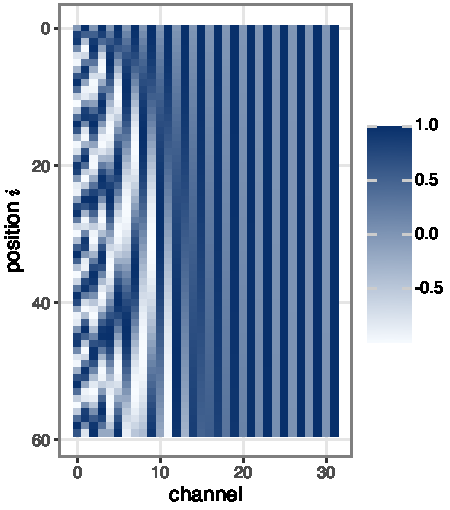
\includegraphics[width=\linewidth]{positional_encoding.pdf}
    \caption{}
  \end{subfigure}\hfill
  \begin{subfigure}[b]{0.45\linewidth}
    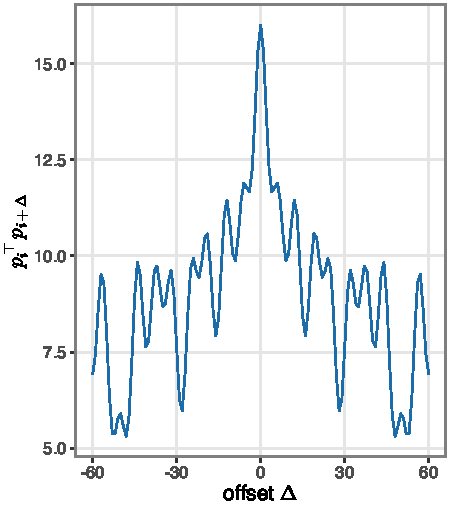
\includegraphics[width=\linewidth]{positional_dot.pdf}
    \caption{}
  \end{subfigure}
  \caption{Sinusoidal positional encoding for $L=60$ positions and $D=32$ channels, $b=10^4$. (a) The encoding matrix; row $i$ is $\vp_i$. (b) The inner product $\vp_i^\top\vp_{i+\Delta}$ depends only on the offset $\Delta$ and peaks at $\Delta=0$.}
  \label{fig:posenc}
\end{figure}

Adding the encoding to the input, rather than concatenating it, may seem to corrupt the input signal. Concatenation works too, but addition is simpler and works as well in practice: in high dimension, the model can learn to keep content and position in nearly separate subspaces. With the encoding added, the score between positions $i$ and $j$ expands into four terms,
\begin{equation}
  \vq_i^\top\vk_j = (\mW^Q\ve_i + \mW^Q\vp_i)^\top(\mW^K\ve_j + \mW^K\vp_j),
\end{equation}
where $\ve_i=\mW^{\text{in}}\vx_i$ is the content embedding: a content-content term, two content-position terms and a position-position term, the last of which lets the model favour nearby positions. Learned positional embeddings, one free vector $\vp_i$ per position, are an alternative. Enformer uses \emph{relative} positional encodings, which add to each score $s_{ij}$ a learned function of the offset $j-i$ built from fixed basis functions of distance~\citep{avsec2021}.

\subsection{Rotary positional embeddings}

Many recent transformers use rotary positional embeddings (RoPE)~\citep{su2024}, which build the offset-only property directly into the scores. In this subsection we write $m$ and $n$ for the positions of a query and a key. In two dimensions, let $\mR(\alpha)$ be the matrix that rotates a vector by angle $\alpha$,
\begin{equation}
  \mR(\alpha) = \begin{pmatrix}\cos\alpha & -\sin\alpha\\ \sin\alpha & \cos\alpha\end{pmatrix},
\end{equation}
and rotate the query at position $m$ and the key at position $n$ by angles proportional to their positions, $\tilde\vq_m=\mR(m\theta)\vq_m$ and $\tilde\vk_n=\mR(n\theta)\vk_n$, for a frequency $\theta$. Rotations compose by adding angles and $\mR(\alpha)^\top=\mR(-\alpha)$, so $\mR(m\theta)^\top\mR(n\theta)=\mR((n-m)\theta)$ and
\begin{equation}
  \tilde\vq_m^\top\tilde\vk_n = \vq_m^\top\mR(m\theta)^\top\mR(n\theta)\vk_n = \vq_m^\top\mR\big((n-m)\theta\big)\vk_n .
\end{equation}
The score depends on the content of the query and key and on their offset $n-m$, but not on their absolute positions. For $P$ dimensions, split the query and key into $P/2$ pairs of coordinates and rotate pair $r=0,\dots,P/2-1$ by its own frequency $\theta_r=b^{-2r/P}$, as in the sinusoidal encoding: $\mR_m=\operatorname{blockdiag}(\mR(m\theta_0),\dots,\mR(m\theta_{P/2-1}))$. The fastest pair rotates by one radian per position, a full turn about every 6 positions; with $b=10^4$, the slowest takes around $2\pi\times10^4\approx63{,}000$ positions. The same construction is often described with complex numbers: treating a pair of coordinates as a complex number, a rotation is multiplication by a unit complex number, and the score is the real part of a product in which the two position-dependent phases cancel to leave only their difference. Unlike additive encodings, RoPE leaves the values unchanged and acts only on the scores.

%======================================================================
\section{Three-dimensional genome organization}
\label{sec:hic}
%======================================================================

Enhancers regulate genes through chromatin loops, so a model that predicts gene regulation from sequence would benefit from knowing how the genome folds. Chromosome conformation capture (3C)~\citep{dekker2002} and its successors 4C and 5C measure contacts between chosen genomic regions. \emph{Hi-C}~\citep{lieberman2009} measures contacts between all pairs of regions genome-wide (Figure~\ref{fig:hic_protocol}). Chromatin is crosslinked, so that DNA segments close together in three dimensions are held together by proteins, and digested with a restriction enzyme. The cut ends are filled in with biotin-labelled nucleotides and ligated, joining segments that were close in space even if they are far apart, or on different chromosomes, in the linear genome. After reversing the crosslinks and shearing the DNA, the biotinylated junctions are pulled down with streptavidin and sequenced with paired-end reads. Each read pair whose two ends map to distant locations records a contact. Counting read pairs for every pair of genomic bins gives a symmetric \emph{contact matrix}. Because the number of bin pairs grows quadratically with resolution, Hi-C requires a very large number of reads.

\begin{figure}[t]
  \centering
  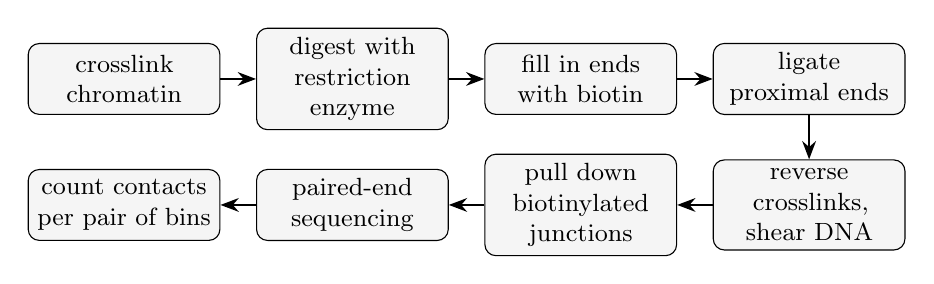
\begin{tikzpicture}[>=Stealth, every node/.style={font=\small, align=center}, st/.style={draw, rounded corners, fill=gray!8, minimum height=0.9cm, text width=2.2cm}]
    \node[st] (s1) at (0,0) {crosslink\\chromatin};
    \node[st] (s2) at (2.9,0) {digest with\\restriction enzyme};
    \node[st] (s3) at (5.8,0) {fill in ends\\with biotin};
    \node[st] (s4) at (8.7,0) {ligate\\proximal ends};
    \node[st] (s5) at (8.7,-1.6) {reverse crosslinks,\\shear DNA};
    \node[st] (s6) at (5.8,-1.6) {pull down\\biotinylated\\junctions};
    \node[st] (s7) at (2.9,-1.6) {paired-end\\sequencing};
    \node[st] (s8) at (0,-1.6) {count contacts\\per pair of bins};
    \foreach \a/\b in {s1/s2,s2/s3,s3/s4,s4/s5,s5/s6,s6/s7,s7/s8} \draw[->, thick] (\a) -- (\b);
  \end{tikzpicture}
  \caption{The Hi-C protocol. Ligation joins DNA segments that are close in three-dimensional space; sequencing the junctions and mapping both ends gives counts of contacts between every pair of genomic bins.}
  \label{fig:hic_protocol}
\end{figure}

\subsection{Topologically associating domains}

The strongest signal in a contact matrix is along the diagonal: contact frequency decays with linear distance, roughly as its inverse at the megabase scale~\citep{lieberman2009}. On top of this decay, Hi-C maps show squares along the diagonal (Figure~\ref{fig:hic}a). These are \emph{topologically associating domains} (TADs)~\citep{dixon2012}: regions, typically hundreds of kilobases to around a megabase long, whose loci contact each other much more often than they contact loci in neighbouring domains. A useful picture is DNA wrapped around nucleosomes at the scale of hundreds of base pairs, folded into loops, and packed into largely separate globules at the scale of a megabase. TAD boundaries are often bound by CTCF, and loops anchored at pairs of CTCF sites, held by cohesin, are a common feature~\citep{rao2014}. TADs are largely shared across cell types and are conserved between mouse and human~\citep{dixon2012}. Because enhancers mostly contact genes in the same TAD, TADs constrain which genes an enhancer can regulate.

\citet{dixon2012} called TADs with a \emph{directionality index}. For bin $i$, let $A_i$ be the number of contacts with bins in a window upstream and $B_i$ the number with bins in an equal window downstream, and let $E_i=(A_i+B_i)/2$. Then
\begin{equation}
  \text{DI}_i = \operatorname{sign}(B_i-A_i)\left[\frac{(A_i-E_i)^2}{E_i} + \frac{(B_i-E_i)^2}{E_i}\right],
\end{equation}
a signed chi-squared statistic for the null hypothesis that contacts are equally likely upstream and downstream. Just inside the start of a TAD, a bin contacts mostly downstream bins and the index is positive; near the end of a TAD it is negative. TAD boundaries are where the index switches from negative to positive (Figure~\ref{fig:hic}b). The authors segmented the index with a hidden Markov model, a model we meet in a later chapter.

\begin{figure}[t]
  \centering
  \begin{subfigure}[b]{0.46\linewidth}
    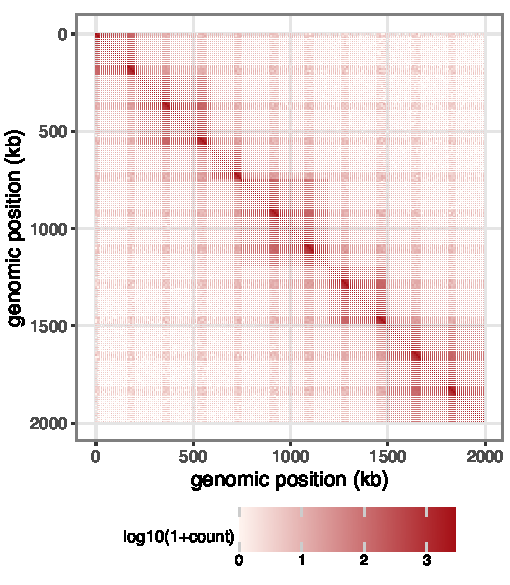
\includegraphics[width=\linewidth]{hic_map.pdf}
    \caption{}
  \end{subfigure}\hfill
  \begin{subfigure}[b]{0.46\linewidth}
    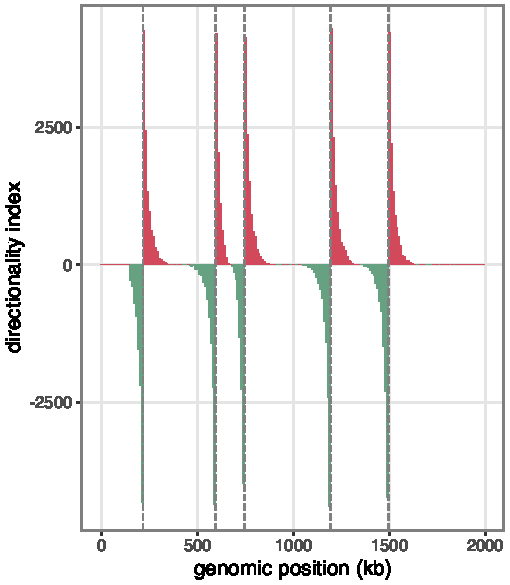
\includegraphics[width=\linewidth]{hic_di.pdf}
    \caption{}
  \end{subfigure}
  \caption{Simulated Hi-C data for 2\,Mb at 10\,kb resolution. Expected contacts decay as the inverse of distance and are seven times higher within TADs; counts are Poisson. (a) The contact matrix shows TADs as squares along the diagonal. (b) The directionality index, with a window of 150\,kb, is positive (downstream bias) at the start of each TAD and negative (upstream bias) at its end; dashed lines mark the true boundaries.}
  \label{fig:hic}
\end{figure}

%======================================================================
\section{Long-range sequence-to-function models}
\label{sec:enformer}
%======================================================================

\subsection{From Basset to Basenji}

Basset classified 600\,bp sequences as accessible or not. Its successor, Basenji~\citep{kelley2018}, predicts the read coverage of thousands of genomic \emph{tracks}, the signal of each ChIP-seq, DNase-seq, ATAC-seq or CAGE experiment along the genome, from about 131\,kb of sequence, in bins of 128\,bp. CAGE (cap analysis of gene expression) measures transcription at transcription start sites, so predicting CAGE at a gene's TSS amounts to predicting its expression. Basenji used dilated convolutions to enlarge its receptive field (Section~\ref{sec:receptive}), and a later version trained jointly on human and mouse data improved predictions in both species~\citep{kelley2020}. Training on several species helps because what these models need is diversity of sequence: human genomes differ from each other at only about one position in a thousand, so more human samples add little new sequence, whereas the mouse genome provides many new examples of regulatory sequence with conserved TFs.

\subsection{Enformer}

Enformer~\citep{avsec2021}, short for enhancer transformer, replaced most of Basenji's dilated convolutions with transformer blocks (Figure~\ref{fig:enformer}). Its input is about 200\,kb (196,608\,bp) of one-hot sequence. Seven convolutional blocks with pooling extract local features, the ``words'' of regulatory sequence, and reduce the sequence to one vector per 128\,bp bin. Eleven transformer blocks with multi-head attention then let each bin draw on every other bin, which can capture the ``grammar'' of interactions between distant elements. Organism-specific output heads predict 5,313 human and 1,643 mouse tracks for the central bins. Enformer can use sequence up to about 100\,kb away from a position, compared with about 20\,kb for Basenji2. Training minimizes a Poisson negative log likelihood of the observed coverage $y_{bt}$ in bin $b$ and track $t$ given the prediction $\hat y_{bt}>0$, which up to a constant is $\sum_{b,t}(\hat y_{bt}-y_{bt}\log\hat y_{bt})$. The data are split into training, validation and test sets by genomic region, so the test set contains regions of the genome the model has not seen.

\begin{figure}[t]
  \centering
  \begin{subfigure}[b]{0.32\linewidth}
    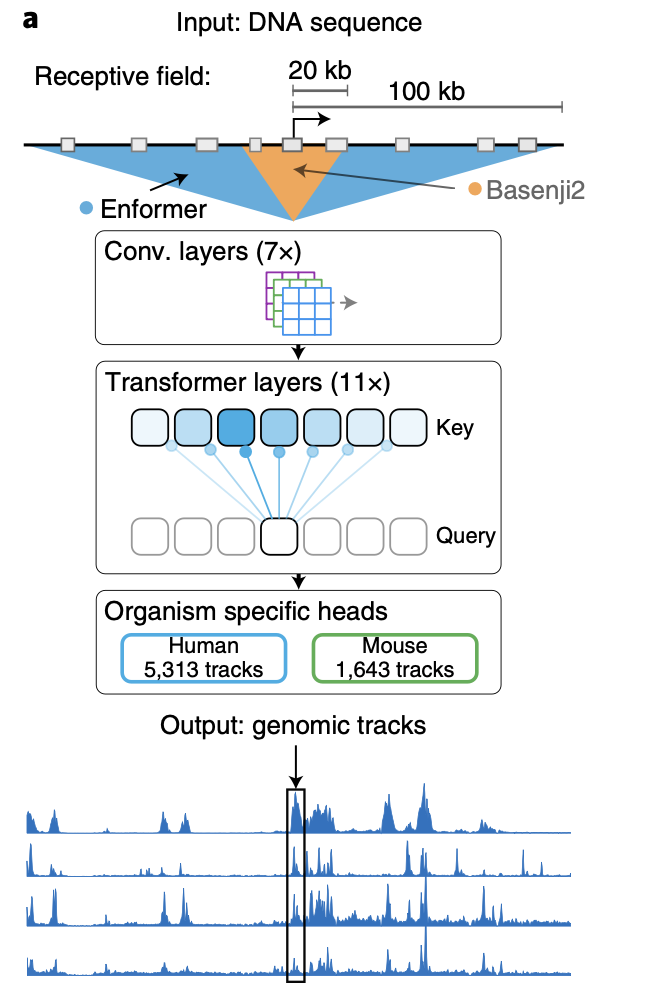
\includegraphics[width=\linewidth]{slides/enformer_architecture.png}
    \caption{}
  \end{subfigure}\hfill
  \begin{subfigure}[b]{0.66\linewidth}
    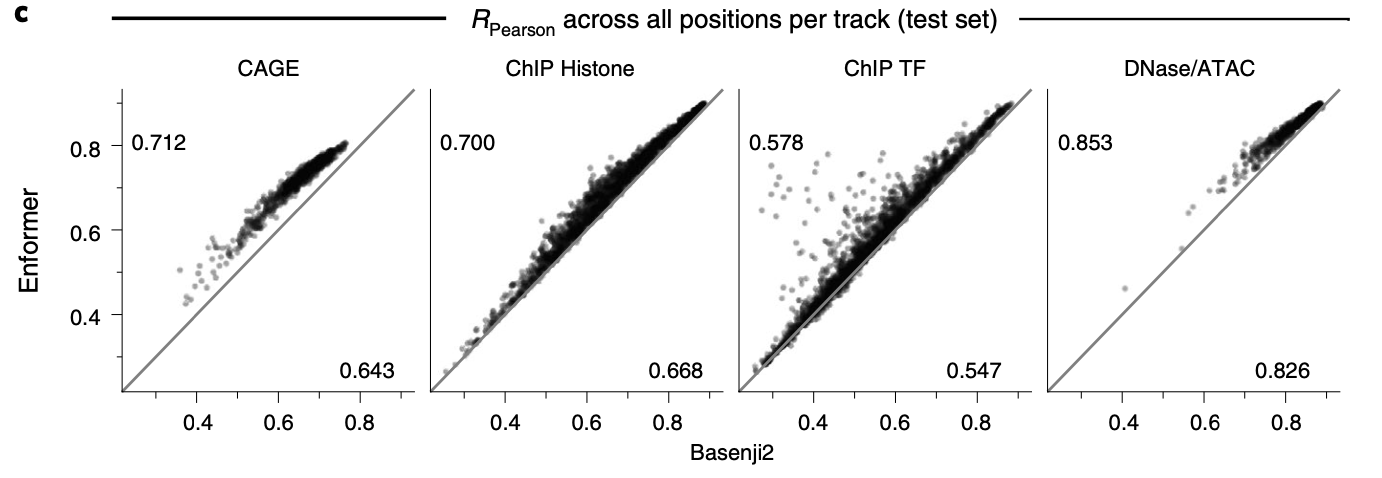
\includegraphics[width=\linewidth]{slides/enformer_performance.png}
    \caption{}
  \end{subfigure}
  \caption{Enformer. (a) Architecture: convolutional layers, transformer layers, and human and mouse output heads predicting genomic tracks; the receptive field (blue) is about five times that of Basenji2 (orange). (b) Pearson correlation between predicted and observed coverage per test-set track, Enformer against Basenji2, for CAGE, histone ChIP-seq, TF ChIP-seq and DNase/ATAC-seq tracks; mean correlations are shown in the corners. Reproduced from \citet{avsec2021}.}
  \label{fig:enformer}
\end{figure}

Performance is measured, for each track, as the Pearson correlation between predicted and observed coverage across all bins of the test regions. Enformer improved on Basenji2 for every class of track (Figure~\ref{fig:enformer}b), with mean correlations rising from 0.643 to 0.712 for CAGE, 0.668 to 0.700 for histone marks, 0.547 to 0.578 for TF binding and 0.826 to 0.853 for accessibility. The gains are modest on average but consistent, and largest for gene expression (CAGE), where distal enhancers matter most. Figure~\ref{fig:enformer_tracks} shows predicted and observed DNase-seq tracks around the immune gene \textit{CD44} in two cell types: Enformer's predictions follow the cell-type-specific peaks more closely than Basenji2's.

\begin{figure}[t]
  \centering
  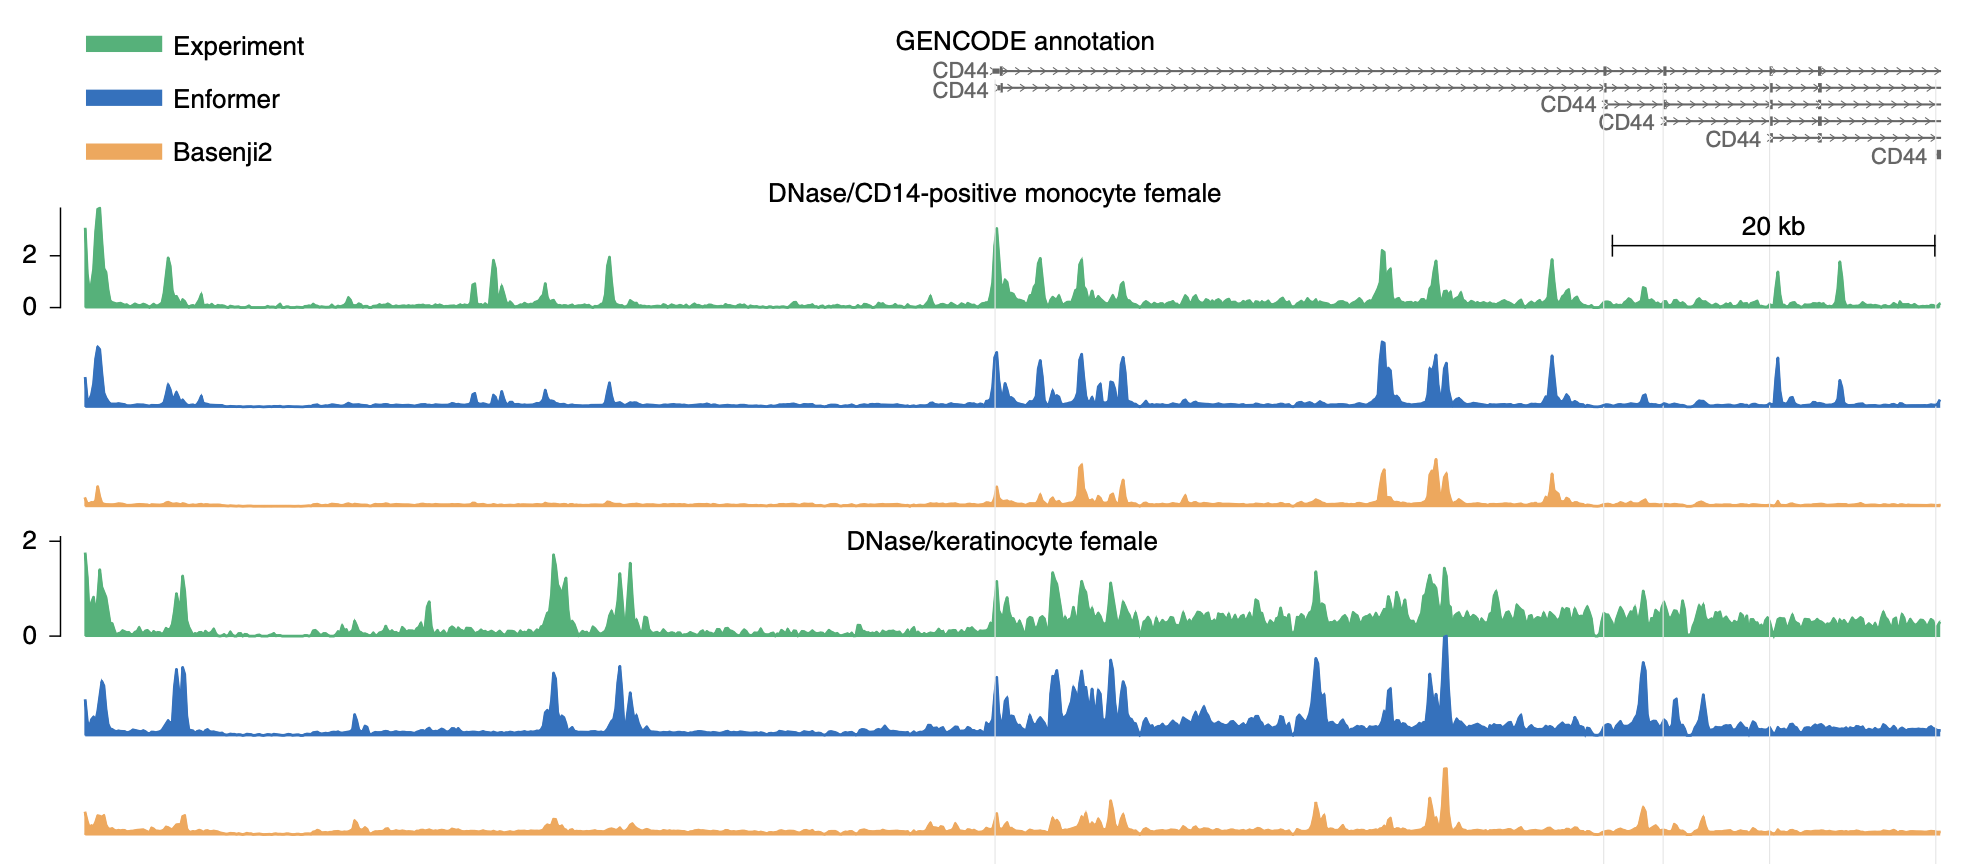
\includegraphics[width=0.85\linewidth]{slides/enformer_tracks.png}
  \caption{Observed (green) and predicted (blue, Enformer; orange, Basenji2) DNase-seq coverage around \textit{CD44} in CD14-positive monocytes and keratinocytes. Reproduced from \citet{avsec2021}.}
  \label{fig:enformer_tracks}
\end{figure}

\subsection{Enformer attends within TADs}

Enformer is trained only on DNA sequence and one-dimensional tracks; it never sees Hi-C data. Yet its attention weights reflect TADs (Figure~\ref{fig:enformer_tad}). Averaging the attention matrices over sequences centred on TAD boundaries, and subtracting the average for sequences centred at random positions, shows that queries attend less to keys on the other side of a boundary and more to keys within their own TAD, and that keys at the boundary itself receive extra attention. A plausible explanation is that the sequence relevant to a gene's expression, its enhancers, lies mostly in the same TAD, and that TAD boundaries have sequence determinants, such as CTCF sites, that the model can recognize. The model learned a feature of three-dimensional genome organization because it was useful for its prediction task, an example of representation learning: models trained on enough data can capture structure they were never explicitly given.

\begin{figure}[t]
  \centering
  \begin{subfigure}[b]{0.42\linewidth}
    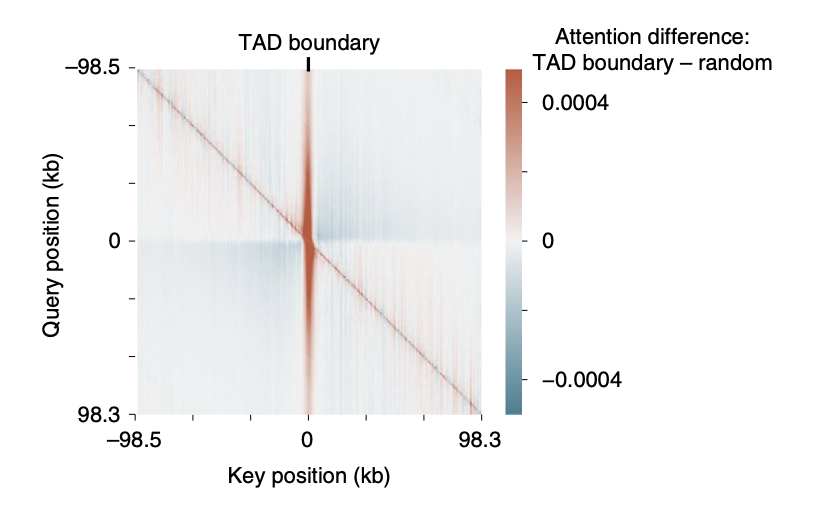
\includegraphics[width=\linewidth]{slides/enformer_tad_attention_map.png}
    \caption{}
  \end{subfigure}\hfill
  \begin{subfigure}[b]{0.55\linewidth}
    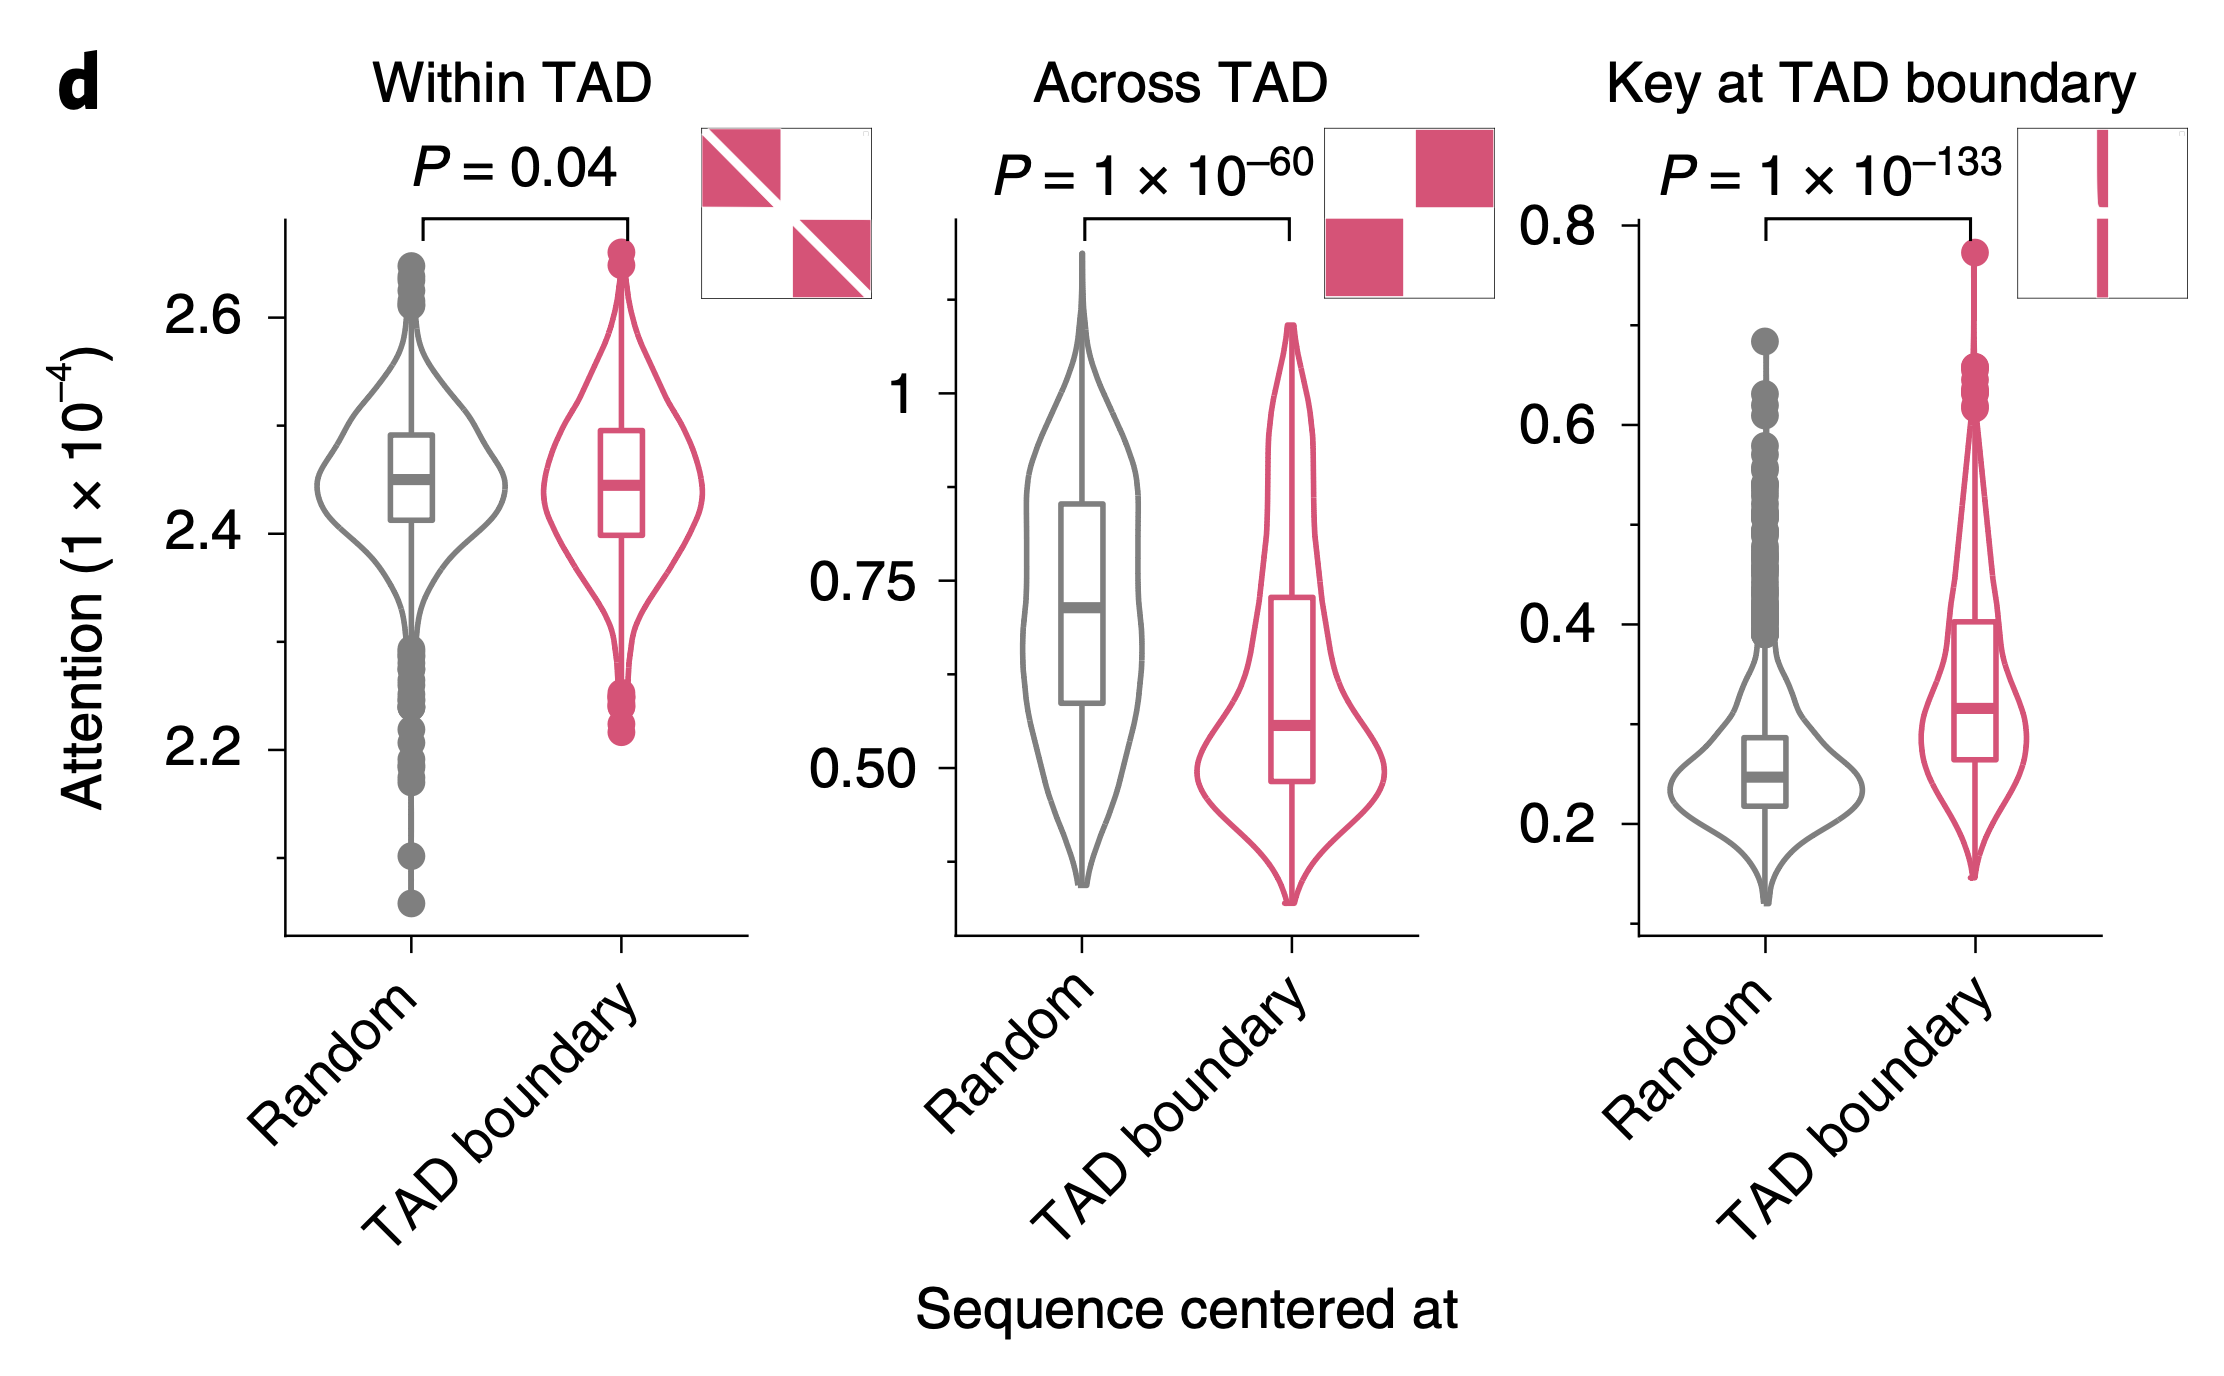
\includegraphics[width=\linewidth]{slides/enformer_tad_attention_violin.png}
    \caption{}
  \end{subfigure}
  \caption{Enformer's attention reflects TADs. (a) Average attention for sequences centred on a TAD boundary minus that for sequences centred at random positions, by query and key position. (b) Average attention within a TAD, across TADs, and to keys at the boundary, for sequences centred at TAD boundaries and at random positions. Reproduced from \citet{avsec2021}.}
  \label{fig:enformer_tad}
\end{figure}

\subsection{AlphaGenome}

AlphaGenome~\citep{avsec2026} extends this approach (Figure~\ref{fig:alphagenome}). Its input is 1\,Mb of sequence, five times Enformer's, and it predicts 5,930 human and 1,128 mouse tracks, many at single base-pair resolution. Beyond Enformer's assays it predicts RNA-seq coverage, PRO-cap, splice sites, splice junctions and splice site usage, and Hi-C-derived contact maps at 2\,kb resolution, so it is trained on three-dimensional structure rather than having to infer it. The architecture follows a U-Net pattern: convolutional encoders shorten the sequence, transformers operate on the shortened sequence, and decoders restore base-pair resolution, with the 1\,Mb sequence partitioned across several interconnected accelerators. Training has two stages. Models are first pre-trained on the observed tracks, either with folds of the genome held out for evaluation or on the whole genome, with data augmentation by random shifts of the input window and reverse complementing. A single student model is then distilled from an ensemble of whole-genome teacher models, trained to reproduce their predictions on sequences with random shifts, reverse complementing and random mutations. A primary aim is predicting the effects of genetic variants, by comparing predictions for the reference and alternative alleles as in Section~\ref{sec:ism}.

\begin{figure}[t]
  \centering
  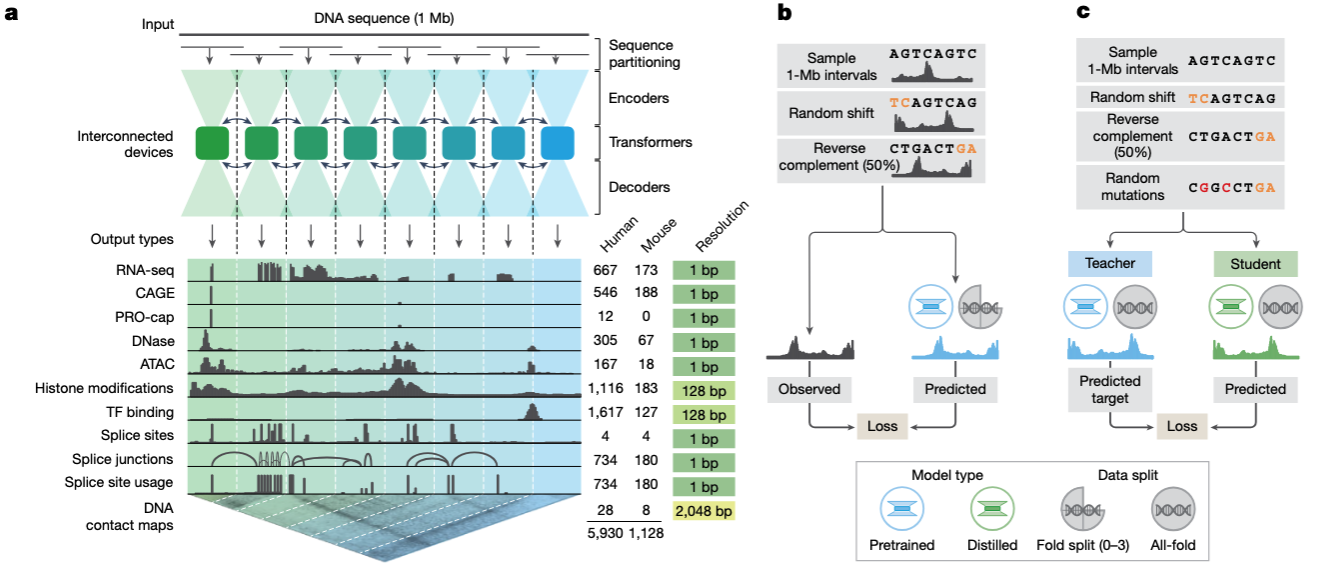
\includegraphics[width=\linewidth]{slides/alphagenome.png}
  \caption{AlphaGenome. (a) A 1\,Mb input sequence is processed by encoders, transformers and decoders distributed across interconnected devices to predict many output types, with the number of human and mouse tracks and the output resolution of each. (b) Pre-training on observed tracks with augmented input sequences. (c) Distillation of a student model from teacher predictions. Reproduced from \citet{avsec2026}.}
  \label{fig:alphagenome}
\end{figure}

%======================================================================
\section{Summary}
%======================================================================

\begin{itemize}
  \item Nearly all cells in the body share the same DNA but differ in which genes they express. Epigenomic assays, histone modification ChIP-seq and chromatin accessibility measured by DNase-seq or ATAC-seq, reveal which regions of the genome are active in each cell type.
  \item Regulatory elements control gene expression. Promoters lie at the gene; enhancers lie further away along the linear genome but are brought close to their target promoters by chromatin loops. Enhancers integrate activating and repressive TF inputs, as in the \textit{eve} stripe 2 enhancer.
  \item ENCODE and Roadmap Epigenomics mapped these signals across hundreds of cell types. The data form a sparse tensor (position $\times$ assay $\times$ cell type) with problems of denoising, imputation and annotation. How much of the biochemically active genome is functional remains debated.
  \item CNNs such as Basset predict accessibility from sequence across many cell types, outperform k-mer methods, learn known TF motifs in their first layer, and predict the effects of genetic variants by in silico mutagenesis.
  \item Attention computes, for every pair of positions, a weight from the inner product of a query and a key, normalized by a softmax, and averages values with these weights: $\mG=\softmax(\mQ\mK^\top/\sqrt{P})\mV$. It connects any two positions in one layer at a cost quadratic in sequence length. Multi-head attention runs several attention patterns in parallel. Attention is permutation equivariant, so positional information is added through sinusoidal, relative or rotary encodings.
  \item Hi-C measures three-dimensional contacts and reveals TADs. Enformer, a convolutional and transformer model with a 200\,kb input, improves track prediction over convolutional models and learns to attend within TADs without seeing Hi-C data. AlphaGenome extends the input to 1\,Mb and adds outputs including splicing and contact maps.
\end{itemize}

%======================================================================
\section*{Exercises}
%======================================================================

\begin{enumerate}
  \item Show that if the entries of $\vq,\vk\in\R^P$ are independent with mean zero and variance one, then $\vq^\top\vk$ has mean zero and variance $P$. Compute the Jacobian of the softmax and show that its entries approach zero as one input becomes much larger than the others.
  \item Write out the shapes of every matrix in multi-head attention with $L$ positions, $D$ channels and $M$ heads, and count the parameters of the layer. Show that the cost of computing the attention matrices is $O(ML^2P)$.
  \item Prove that self-attention without positional information is permutation equivariant. Show that adding the sinusoidal encoding breaks this symmetry, and that $\vp_{i+\Delta}$ is obtained from $\vp_i$ by a rotation of each pair of channels that does not depend on $i$.
  \item Show that a convolution of odd width $k$ with $D$ input and output channels can be written as a sum over offsets of $D\times D$ matrices applied to shifted inputs, and that self-attention with $a_{ij}$ fixed to $1/k$ when $|i-j|\leq(k-1)/2$ and zero otherwise is a special case with all $k$ matrices equal to $\mW^V/k$. What does the convolution gain from having separate matrices per offset?
  \item Compute the receptive field, in base pairs, of a network with seven convolutional layers of width 5, each followed by max pooling of width 2. How many such layers would be needed to reach 100\,kb, and what would the output resolution be?
  \item Simulate a Hi-C contact matrix with TADs as in Figure~\ref{fig:hic}, compute the directionality index, and call boundaries where it changes sign from negative to positive. How does the accuracy of the calls change with the sequencing depth and the window size?
\end{enumerate}

\bibliographystyle{abbrvnat}
\bibliography{../chapter03/chapter03}
\endgroup

% Generated wrapper: chapter 04 with its own figure path, macros and bibliography.
\graphicspath{{../chapter04/figures/}}
\makeatletter\def\input@path{{../chapter04/}}\makeatother
\begingroup
% Chapter 4: interpreting neural networks.
% Requires: amsmath, amssymb, bm, graphicx, booktabs, multirow, subcaption, algorithm, algpseudocode,
% tikz (arrows.meta, positioning, calc, decorations.pathreplacing, shapes.geometric, fit), natbib.
% Computed figures are produced by scripts/make_figures.py; figures/slides/ holds figures taken from the lecture slides.

\providecommand{\R}{\mathbb{R}}
\providecommand{\E}{\mathbb{E}}
\providecommand{\Normal}{\mathcal{N}}
\providecommand{\argmax}{\operatorname*{arg\,max}}
\providecommand{\argmin}{\operatorname*{arg\,min}}
\providecommand{\vy}{\mathbf{y}}
\providecommand{\vx}{\mathbf{x}}
\providecommand{\mX}{\mathbf{X}}
\providecommand{\mI}{\mathbf{I}}
\providecommand{\vb}{\boldsymbol{\beta}}
\providecommand{\veps}{\boldsymbol{\epsilon}}
\providecommand{\vp}{\mathbf{p}}
\providecommand{\vg}{\mathbf{g}}
\providecommand{\ind}{\mathbf{1}}
\providecommand{\vz}{\mathbf{z}}
\providecommand{\vh}{\mathbf{h}}
\providecommand{\vw}{\mathbf{w}}
\providecommand{\vs}{\mathbf{s}}
\providecommand{\ve}{\mathbf{e}}
\providecommand{\mW}{\mathbf{W}}
\providecommand{\relu}{\operatorname{ReLU}}
\providecommand{\IG}{\operatorname{IG}}

% TikZ styles shared by the network diagrams in this chapter
\tikzset{
  nn/.style={circle, draw, fill=blue!12, minimum size=7mm, inner sep=0pt, font=\scriptsize},
  nnr/.style={nn, fill=red!30},
  nny/.style={nn, fill=yellow!70},
  nnb/.style={draw, rectangle, minimum size=4mm, inner sep=1pt, font=\scriptsize, fill=white},
  wlab/.style={font=\tiny, fill=white, inner sep=0.6pt},
  lyr/.style={font=\scriptsize, anchor=east, text=black!70},
}

\providecommand{\chaptertoc}{}
\chapter{Interpreting neural networks}
\label{ch:interpretation}
\chaptertoc

The convolutional networks and transformers of Chapters 2 and 3 predict chromatin accessibility, transcription factor binding and gene expression from DNA sequence with high accuracy. Accuracy alone, however, is rarely the end goal in genomics. If a model predicts that a sequence is an active enhancer, we want to know \emph{why}: which nucleotides drive the prediction, which transcription factor motifs they correspond to, and how a mutation at a given position would change the output. This chapter develops methods that answer these questions for a trained network. They assign an importance score to each input feature, for example each nucleotide, for one prediction at a time. We start from the most intuitive approach, perturbing the input and observing the output, and then derive a sequence of increasingly principled methods based on backpropagation: gradients, deconvolutional networks, guided backpropagation, DeepLIFT and integrated gradients. We close with Shapley values, which provide a theoretical framework that connects several of these methods.

%======================================================================
\section{Why interpret a neural network?}
\label{sec:why_interpret}
%======================================================================

There is a broad trade-off between the predictive power of a method and how easily we can interpret it (Figure~\ref{fig:power_interp}). Classical statistical models, such as the linear and L1-regularized regression of Chapter 1, are interpretable: each feature has a coefficient, and features with large coefficients matter. Traditional machine learning methods, such as support vector machines and random forests, are often more accurate, particularly on tabular data, but are harder to interpret. Deep neural networks, which may have billions of parameters and many layer types, are typically the most accurate on sequence data, and they learn useful representations of the data that would be difficult to engineer by hand. They are also the hardest to understand, and their ``black box'' nature is a common criticism~\citep{castelvecchi2016}. Suppose we train a model to predict which DNA mutations cause a disease. If the model performs well, it has likely learned patterns that we would also like to understand. The aim of interpretation methods is to keep the power of deep learning while recovering some of the insight that simpler models give for free.

\begin{figure}[t]
  \centering
  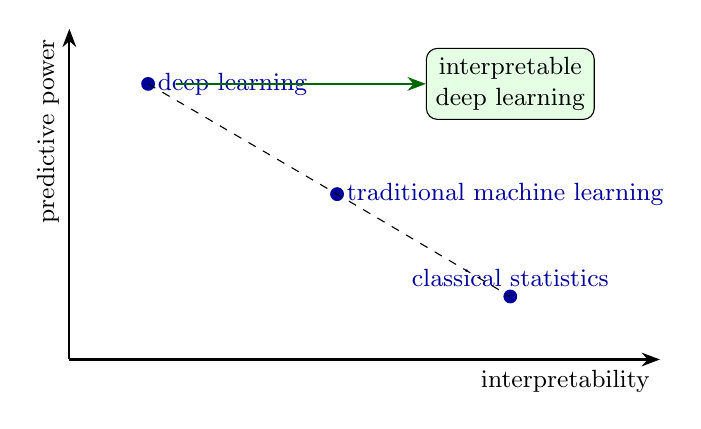
\begin{tikzpicture}[>=Stealth, every node/.style={font=\small}]
    \draw[->, thick] (0,0) -- (7.5,0) node[below left] {interpretability};
    \draw[->, thick] (0,0) -- (0,4.2) node[above left, rotate=90, anchor=south east] {predictive power};
    \fill[blue!60!black] (1.0,3.5) circle (2.5pt) node[right] {deep learning};
    \fill[blue!60!black] (3.4,2.1) circle (2.5pt) node[right] {traditional machine learning};
    \fill[blue!60!black] (5.6,0.8) circle (2.5pt) node[above] {classical statistics};
    \draw[dashed] (1.0,3.5) -- (3.4,2.1) -- (5.6,0.8);
    \node[draw, rounded corners, fill=green!10, align=center] (goal) at (5.6,3.5) {interpretable\\deep learning};
    \draw[->, thick, green!40!black] (1.35,3.5) -- (goal.west);
  \end{tikzpicture}
  \caption{The trade-off between predictive power and interpretability. Interpretation methods aim to move deep learning models to the right without losing power.}
  \label{fig:power_interp}
\end{figure}

\subsection{What would we like to know?}

Before introducing methods, it helps to list the ways one might try to understand how a trained network makes its predictions.
\begin{itemize}
  \item \emph{Look at the learned parameters.} For a simple network this can work. The first-layer convolutional filters of the Basset model~\citep{kelley2016} (Chapter 3) resemble the position weight matrices of known transcription factor motifs. Deeper layers combine filters in ways that are much harder to read off, and even first-layer filters do not always correspond to clean motifs.
  \item \emph{Ablation.} Remove or zero out an input feature, a filter or an internal node, and measure the change in performance. Done across the whole data set this gives a \emph{global} measure of importance; done for one data point it measures how much a single prediction depends on that component. Ablation is related to stepwise regression in classical statistics: forward stepwise regression starts with no features and repeatedly adds the most useful one, while backward stepwise regression starts with all features and repeatedly removes the least useful.
  \item \emph{Attention weights.} For transformers, the attention matrices show which positions each position attends to. The Enformer model~\citep{avsec2021} was shown to attend to topologically associating domain (TAD) boundaries in this way (Chapter 3). With many layers and many heads per layer, though, the attention weights must be aggregated in some ad hoc way, typically averaged, which makes them harder to interpret.
  \item \emph{Saliency maps.} Ask how much a small change to each input feature would change the output for one data point. This can be computed by perturbation (in silico mutagenesis) or by backpropagation (gradients). It is a \emph{local} measure: it describes the model near one input.
  \item \emph{Local linearization.} We know how to interpret a linear model. Replacing the whole network by a linear model would defeat the purpose of using a network, but we can approximate it by a linear model \emph{near} a given data point and interpret that approximation. Gradients do exactly this, and we will see that several other methods can be viewed as better-behaved linearizations.
  \item \emph{Input optimization.} Find inputs that maximize or minimize the output. Unconstrained, the optimal input is often unnatural and not very informative. A more useful variant starts from a real data point and asks how it could be changed to increase or decrease the prediction.
\end{itemize}
Most of this chapter is about \emph{local feature attribution}: given a trained model and one input, assign a score to each input feature that reflects its importance for that prediction (Figure~\ref{fig:attribution_task}). Scores for many inputs can then be aggregated, for example by clustering high-scoring subsequences into motifs, to give a global picture.

\begin{figure}[t]
  \centering
  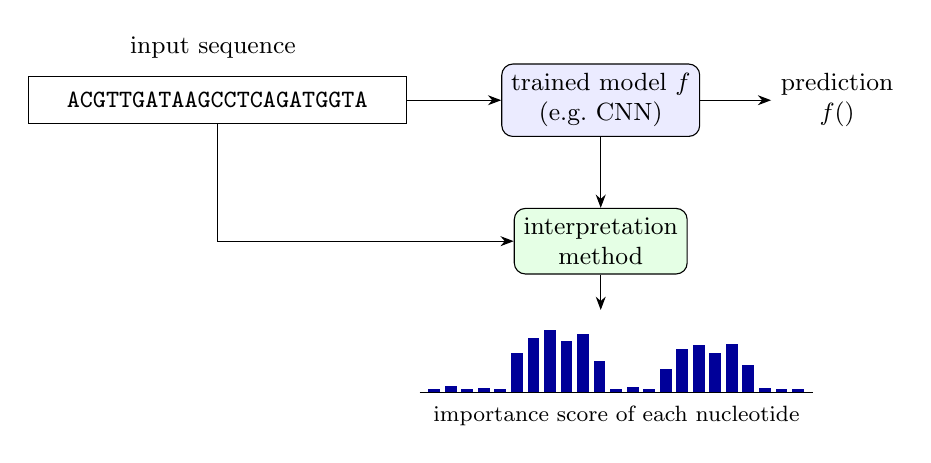
\begin{tikzpicture}[>=Stealth, every node/.style={font=\small, align=center}]
    \node[draw, minimum width=4.8cm, minimum height=0.6cm, font=\ttfamily\small] (seq) {ACGTTGATAAGCCTCAGATGGTA};
    \node[above=0.1cm of seq] {input sequence $\vx$};
    \node[draw, rounded corners, fill=blue!8, right=1.2cm of seq] (model) {trained model $f$\\(e.g.\ CNN)};
    \node[right=0.9cm of model] (pred) {prediction\\$f(\vx)$};
    \draw[->] (seq) -- (model); \draw[->] (model) -- (pred);
    \node[draw, rounded corners, fill=green!10, below=0.9cm of model] (meth) {interpretation\\method};
    \draw[->] (model) -- (meth); \draw[->] (seq.south) |- (meth.west);
    \begin{scope}[shift={($(meth.south)+(-2.4,-1.5)$)}]
      \foreach \h [count=\i] in {0.05,0.08,0.04,0.06,0.05,0.5,0.7,0.8,0.65,0.75,0.4,0.05,0.07,0.04,0.3,0.55,0.6,0.5,0.62,0.35,0.06,0.04,0.05}
        \fill[blue!60!black] ({0.21*\i},0) rectangle ({0.21*\i+0.15},\h);
      \draw (0.1,0) -- (5.1,0);
      \node[below, font=\footnotesize] at (2.6,-0.05) {importance score of each nucleotide};
    \end{scope}
    \draw[->] (meth.south) -- ++(0,-0.45);
  \end{tikzpicture}
  \caption{Local feature attribution. An interpretation method takes a trained model and one input, and returns an importance score for each input feature, here each nucleotide. High-scoring stretches often correspond to transcription factor binding motifs.}
  \label{fig:attribution_task}
\end{figure}

Throughout, let $f:\R^P\to\R$ be the trained network, mapping an input $\vx\in\R^P$ to a scalar output $f(\vx)$, for example the logit of one class or the prediction for one task of a multitask model. For a DNA sequence of length $L$ in one-hot encoding (Chapter 2), the input is a binary $4\times L$ matrix with one non-zero entry per column, which we flatten to $\vx\in\{0,1\}^P$ with $P=4L$ when convenient; we write $x_{b,l}$ for the entry for base $b\in\{\mathrm{A},\mathrm{C},\mathrm{G},\mathrm{T}\}$ at position $l\in\{1,\dots,L\}$. An attribution method returns a vector of scores $\vs(\vx)\in\R^P$, one per input feature.

%======================================================================
\section{Perturbation and in silico mutagenesis}
\label{sec:perturbation}
%======================================================================

The most direct way to measure the importance of an input feature is to change it and observe how the output changes. One of the earliest examples in computer vision slides a grey square across an image and records the predicted probability of the correct class with the square at each location~\citep{zeiler2014}. Regions where occlusion reduces the probability are important for the prediction (Figure~\ref{fig:occlusion}). Covering the face of the Pomeranian removes the evidence for the dog; covering the wheel reduces the probability of ``car wheel''. In vision we can check such maps against our own perception. Nobody can look at a DNA sequence and recognize a transcription factor binding motif in the same way, which makes reliable interpretation methods more important in genomics, not less.

\begin{figure}[t]
  \centering
  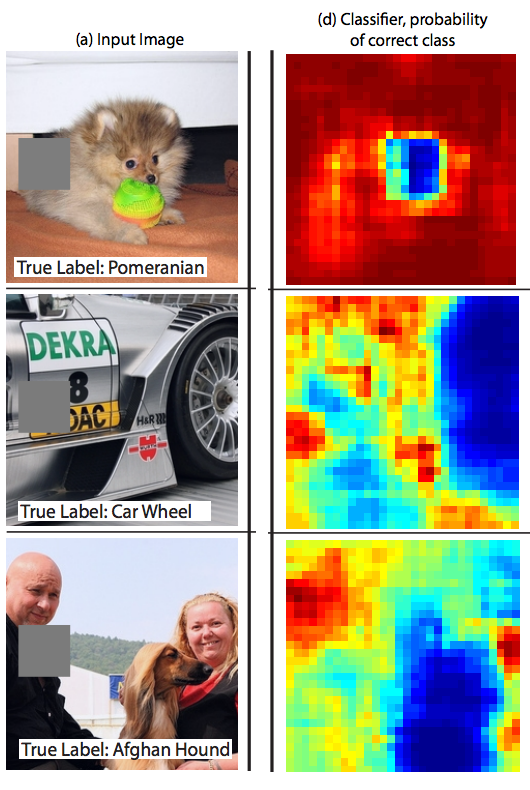
\includegraphics[width=0.36\linewidth]{slides/occlusion_zeiler_fergus.png}
  \caption{Occlusion analysis of an image classifier. Left, input images with the grey occluding square in one of its positions. Right, the probability of the correct class as a function of the position of the square; blue is low. Reproduced from \citet{zeiler2014}.}
  \label{fig:occlusion}
\end{figure}

Other perturbation methods include prediction difference analysis~\citep{zintgraf2017}, which marginalizes over plausible values of each feature rather than setting it to a fixed value, and LIME~\citep{ribeiro2016}, which fits a sparse linear model to the network's outputs on randomly perturbed versions of the input, giving an explicit local linear approximation.

\subsection{In silico mutagenesis}

For DNA sequence the natural perturbation is a point mutation. \emph{In silico mutagenesis} (ISM; ``in silico'' meaning on a computer) mutates each position of the input sequence to each alternative base and records the change in prediction~\citep{alipanahi2015,zhou2015}. Let $\vx^{(l\to b)}$ be the sequence $\vx$ with the base at position $l$ replaced by $b$. ISM computes the $4\times L$ matrix of effects
\begin{equation}
  \Delta_{b,l} = f\big(\vx^{(l\to b)}\big) - f(\vx), \qquad b\in\{\mathrm{A},\mathrm{C},\mathrm{G},\mathrm{T}\},\; l\in\{1,\dots,L\},
  \label{eq:ism}
\end{equation}
where $\Delta_{b,l}=0$ for the observed base. A single importance score per position can be taken as the mean effect of mutating away from the observed base, $s_l = -\frac{1}{3}\sum_{b}\Delta_{b,l}$, which is large when every possible mutation at $l$ reduces the prediction. The full matrix is also useful: it predicts the effect of every possible single-nucleotide variant, which is how models such as Basset and Enformer are used to score genetic variants (Chapter 3).

\subsection{Drawbacks of perturbation}

Perturbation methods have two main drawbacks.

\paragraph{Computational cost.} Each perturbation requires a forward pass through the network. Full ISM of a sequence of length $L$ requires $3L$ forward passes. For a model such as Enformer, whose input is about 200,000 bp long, this is about 600,000 forward passes for a single input sequence, which is expensive even with modern hardware.

\paragraph{Saturation.} Perturbing one feature at a time can miss features that matter only in combination. Consider the function of two inputs $x_1,x_2\in\R$
\begin{equation}
  y = \begin{cases} x_1+x_2 & \text{if } x_1+x_2<1,\\ 1 & \text{if } x_1+x_2\geq 1,\end{cases}
  \qquad\text{that is,}\qquad y=\min(x_1+x_2,\,1),
  \label{eq:sat_fn}
\end{equation}
shown in Figure~\ref{fig:saturation}a. A network with one hidden ReLU unit, $\relu(z)=\max(0,z)$, represents it exactly,
\begin{equation}
  z = -x_1 - x_2 + 1, \qquad h = \relu(z), \qquad y = -h + 1 ,
  \label{eq:sat_net}
\end{equation}
where $z\in\R$ is the pre-activation of the hidden unit, $h\in\R$ its activation, and the two $+1$ terms are intercepts (Figure~\ref{fig:saturation}b). The weights of $-1$ on the inputs flip the ReLU horizontally and the weight of $-1$ on the output flips it vertically, turning a ramp that starts at zero into a ramp that stops at one. At the input $\vx=(1,1)$ we have $z=-1$, $h=0$ and $y=1$. Now perturb $x_1$ to zero: $z=0$, $h=0$ and still $y=1$ (Figure~\ref{fig:saturation}c). The same holds for $x_2$. Moving from $x_1+x_2=2$ to $x_1+x_2=1$ stays on the flat part of the function, so neither single perturbation changes the output, and ISM assigns zero importance to both inputs even though $y$ clearly depends on them: setting both to zero changes $y$ from 1 to 0. Perturbing all subsets of features would detect this, but the number of subsets grows exponentially; even all pairs of positions in a 200,000 bp sequence would require $\sim\!10^{10}$ forward passes. In short, perturbations can be both expensive and too local.

\begin{figure}[t]
  \centering
  \begin{tikzpicture}[>=Stealth, every node/.style={font=\small}]
    % (a) the function
    \begin{scope}
      \node at (-0.4,2.9) {(a)};
      \draw[->] (0,0) -- (3.3,0);
      \node[below] at (2.1,-0.35) {$x_1+x_2$};
      \draw[->] (0,0) -- (0,2.6) node[left] {$y$};
      \draw[very thick, green!50!black] (0,0) -- (1.4,1.4) -- (3.1,1.4);
      \foreach \x/\l in {1.4/1, 2.8/2} \draw (\x,0.05) -- (\x,-0.05) node[below] {\l};
      \draw (0.05,1.4) -- (-0.05,1.4) node[left] {1};
      \node[below left] at (0,0) {0};
      \fill (2.8,1.4) circle (2pt);
      \draw[->, red!70!black, thick] (2.75,1.65) -- (1.5,1.65);
    \end{scope}
    % (b) network at (1,1)
    \begin{scope}[xshift=4.6cm]
      \node at (-0.4,2.9) {(b)};
      \node[nn] (x1) at (0,0) {1}; \node[nn] (x2) at (1.4,0) {1};
      \node[nn] (z) at (0.7,1.2) {$-1$}; \node[nn] (h) at (0.7,2.0) {0}; \node[nn] (y) at (0.7,2.9) {1};
      \node[nnb, right=1mm of z] {$+1$}; \node[nnb, right=1mm of y] {$+1$};
      \draw (x1) -- node[wlab, left] {$-1$} (z); \draw (x2) -- node[wlab, right] {$-1$} (z);
      \draw (z) -- (h); \draw (h) -- node[wlab, left] {$-1$} (y);
      \node[below] at (x1.south) {$x_1$}; \node[below] at (x2.south) {$x_2$};
      \node[lyr] at (-0.2,1.6) {ReLU};
    \end{scope}
    % (c) perturbed
    \begin{scope}[xshift=8.0cm]
      \node at (-0.4,2.9) {(c)};
      \node[nnr] (x1) at (0,0) {0}; \node[nn] (x2) at (1.4,0) {1};
      \node[nn] (z) at (0.7,1.2) {0}; \node[nn] (h) at (0.7,2.0) {0}; \node[nn] (y) at (0.7,2.9) {1};
      \node[nnb, right=1mm of z] {$+1$}; \node[nnb, right=1mm of y] {$+1$};
      \draw (x1) -- node[wlab, left] {$-1$} (z); \draw (x2) -- node[wlab, right] {$-1$} (z);
      \draw (z) -- (h); \draw (h) -- node[wlab, left] {$-1$} (y);
      \node[below] at (x1.south) {$x_1$}; \node[below] at (x2.south) {$x_2$};
      \node[lyr] at (-0.2,1.6) {ReLU};
    \end{scope}
  \end{tikzpicture}
  \caption{The saturation problem. (a) The function $y=\min(x_1+x_2,1)$. (b) A one-unit ReLU network computing it, evaluated at $\vx=(1,1)$; numbers in circles are node values, numbers on edges are weights and boxes are intercepts. (c) Setting $x_1$ to zero (red) moves along the flat part of the function (arrow in a) and leaves the output unchanged, so perturbation assigns $x_1$ no importance.}
  \label{fig:saturation}
\end{figure}

%======================================================================
\section{Gradients and saliency maps}
\label{sec:gradients}
%======================================================================

\subsection{The gradient as a local linear model}

The computational problem of perturbation has an elegant solution. Instead of changing each input and rerunning the network, we compute the gradient of the output with respect to every input in one backward pass. During training (Chapter 2), backpropagation computes the gradient of the loss with respect to the parameters; exactly the same machinery gives the gradient of the output $f(\vx)$ with respect to the inputs $\vx$, or with respect to any intermediate node. This was proposed as a way to visualize image classifiers by \citet{simonyan2014}, who called the result a \emph{saliency map}.

The gradient $\nabla_{\vx}f(\vx)\in\R^P$ is the best local linear approximation of $f$ near $\vx$. By Taylor's theorem, for a small perturbation $\boldsymbol{\delta}\in\R^P$,
\begin{equation}
  f(\vx+\boldsymbol{\delta}) \approx f(\vx) + \nabla_{\vx}f(\vx)^\top\boldsymbol{\delta} = f(\vx) + \sum_{i=1}^P \frac{\partial f}{\partial x_i}(\vx)\,\delta_i .
  \label{eq:taylor}
\end{equation}
Near $\vx$, the network behaves like a linear model with coefficients $\partial f/\partial x_i$, so $|\partial f/\partial x_i|$ measures how sensitive the output is to feature $i$. For one-hot DNA, the gradient also approximates ISM. Mutating position $l$ from the observed base $b$ to $b'$ corresponds to $\boldsymbol{\delta}=\ve_{b',l}-\ve_{b,l}$, where $\ve_{b,l}\in\R^P$ is the indicator vector of base $b$ at position $l$, so
\begin{equation}
  \Delta_{b',l} \approx \frac{\partial f}{\partial x_{b',l}} - \frac{\partial f}{\partial x_{b,l}} .
  \label{eq:ism_approx}
\end{equation}
All $3L$ approximate mutation effects therefore cost one forward and one backward pass, roughly the price of two forward passes, instead of $3L$ forward passes. The approximation is only first order, and a single-base change in a one-hot input is not small, so~\eqref{eq:ism_approx} can be inaccurate where the network is strongly non-linear.

\subsection{Backpropagation through a toy network}

To see what the gradient computes, we work through backpropagation on the small convolution-like network of Figure~\ref{fig:toycnn}a. It has five inputs $\vx\in\R^5$, a first layer of four units each connected to two adjacent inputs, a ReLU, a second layer of two units each connected to three adjacent first-layer units, another ReLU, and a final max over the two remaining units, which plays the role of max pooling. The layers are ``convolution-like'' only in their local connectivity; to keep the arithmetic simple the weights are not shared across positions and all intercepts are zero. Writing $\vz^{(1)}\in\R^4$ and $\vz^{(2)}\in\R^2$ for the pre-activations and $\vh^{(1)}=\relu(\vz^{(1)})$, $\vh^{(2)}=\relu(\vz^{(2)})$ for the activations, the network is
\begin{equation}
  \vz^{(1)} = \mW^{(1)}\vx, \quad \vz^{(2)} = \mW^{(2)}\vh^{(1)}, \quad y = \max\big(h^{(2)}_1, h^{(2)}_2\big),
\end{equation}
with weight matrices $\mW^{(1)}\in\R^{4\times 5}$ and $\mW^{(2)}\in\R^{2\times 4}$,
\begin{equation}
  \mW^{(1)} = \begin{pmatrix} -2 & 2 & 0 & 0 & 0\\ 0 & 1 & -2 & 0 & 0\\ 0 & 0 & -1 & 3 & 0\\ 0 & 0 & 0 & -3 & 4 \end{pmatrix}, \qquad
  \mW^{(2)} = \begin{pmatrix} 1 & -1 & -2 & 0\\ 0 & 1 & 2 & -1 \end{pmatrix}.
\end{equation}
For the input $\vx=(2,1,2,1,1)$ the forward pass gives $\vz^{(1)}=(-2,-3,1,1)$, $\vh^{(1)}=(0,0,1,1)$, $\vz^{(2)}=(-2,1)$, $\vh^{(2)}=(0,1)$ and $y=1$.

\begin{figure}[tbp]
  \centering
  \newcommand{\toycnn}[7]{%
    \foreach \v/\s [count=\i] in {#1} {\edef\tmp{\noexpand\node[\s] (in\i) at ({1.5*(\i-1)},0) {$\v$};}\tmp}
    \foreach \v/\s [count=\i] in {#2} {\edef\tmp{\noexpand\node[\s] (ca\i) at ({1.5*(\i-1)+0.75},1.3) {$\v$};}\tmp}
    \foreach \v/\s [count=\i] in {#3} {\edef\tmp{\noexpand\node[\s] (ra\i) at ({1.5*(\i-1)+0.75},2.3) {$\v$};}\tmp}
    \foreach \v/\s [count=\i] in {#4} {\edef\tmp{\noexpand\node[\s] (cb\i) at ({1.5*\i+0.75},4.1) {$\v$};}\tmp}
    \foreach \v/\s [count=\i] in {#5} {\edef\tmp{\noexpand\node[\s] (rb\i) at ({1.5*\i+0.75},5.1) {$\v$};}\tmp}
    \foreach \v/\s in {#6} {\edef\tmp{\noexpand\node[\s] (top) at (3.0,6.1) {$\v$};}\tmp}
    \foreach \j/\a/\b [evaluate=\j as \k using int(\j+1)] in {1/-2/2, 2/1/-2, 3/-1/3, 4/-3/4} {
      \draw (in\j) -- node[wlab, pos=0.75, left] {$\a$} (ca\j);
      \draw (in\k) -- node[wlab, pos=0.75, right] {$\b$} (ca\j);
      \draw (ca\j) -- (ra\j);
    }
    \draw (ra1) -- node[wlab, pos=0.5, above left] {$1$} (cb1);
    \draw (ra2) -- node[wlab, pos=0.4, left] {$-1$} (cb1);
    \draw (ra3) -- node[wlab, pos=0.85, below=1pt] {$-2$} (cb1);
    \draw (ra2) -- node[wlab, pos=0.85, below=1pt] {$1$} (cb2);
    \draw (ra3) -- node[wlab, pos=0.4, right] {$2$} (cb2);
    \draw (ra4) -- node[wlab, pos=0.5, above right] {$-1$} (cb2);
    \draw (cb1) -- (rb1); \draw (cb2) -- (rb2); \draw (rb1) -- (top); \draw (rb2) -- (top);
    \node[font=\small\bfseries, anchor=west] at (-0.6,6.8) {#7};
  }
  \begin{tikzpicture}[scale=0.74, every node/.append style={transform shape}, wlab/.append style={font=\scriptsize}]
    \begin{scope}
      \toycnn{2/nn,1/nn,2/nn,1/nn,1/nn}{-2/nnr,-3/nnr,1/nn,1/nn}{0/nn,0/nn,1/nn,1/nn}{-2/nnr,1/nn}{0/nn,1/nn}{1/nn}{(a) forward pass}
      \foreach \t/\y in {input/0, linear/1.3, ReLU/2.3, linear/4.1, ReLU/5.1, max/6.1} \node[lyr] at (-0.45,\y) {\t};
    \end{scope}
    \begin{scope}[xshift=7.6cm]
      \toycnn{0/nn,0/nn,-2/nn,9/nn,-4/nn}{0/nnr,0/nnr,2/nn,-1/nn}{0/nn,1/nn,2/nn,-1/nn}{0/nnr,1/nn}{0/nn,1/nn}{1/nn}{(b) gradient}
    \end{scope}
    \begin{scope}[yshift=-7.9cm]
      \toycnn{0/nn,1/nn,-4/nn,6/nn,0/nn}{0/nn,1/nn,2/nn,0/nn}{0/nn,1/nn,2/nn,-1/nny}{0/nn,1/nn}{0/nn,1/nn}{1/nn}{(c) deconvnet}
      \foreach \t/\y in {input/0, linear/1.3, ReLU/2.3, linear/4.1, ReLU/5.1, max/6.1} \node[lyr] at (-0.45,\y) {\t};
    \end{scope}
    \begin{scope}[xshift=7.6cm, yshift=-7.9cm]
      \toycnn{0/nn,0/nn,-2/nn,6/nn,0/nn}{0/nnr,0/nnr,2/nn,0/nn}{0/nn,1/nn,2/nn,-1/nny}{0/nnr,1/nn}{0/nn,1/nn}{1/nn}{(d) guided backpropagation}
    \end{scope}
  \end{tikzpicture}
  \caption{Backpropagation rules on a toy convolution-like network with zero intercepts. Edge labels are weights. (a) Forward pass for the input $\vx=(2,1,2,1,1)$; red nodes have negative pre-activations, so the ReLU above them outputs zero. (b)--(d) Backward passes; each node holds the backpropagated value for that node, starting from 1 at the output, and the bottom row is the score for each input. (b) The gradient zeroes the signal through ReLUs whose forward input was negative (red). (c) The deconvnet instead zeroes negative backward signals at each ReLU (yellow), ignoring the forward pass. (d) Guided backpropagation applies both rules.}
  \label{fig:toycnn}
\end{figure}

The backward pass (Figure~\ref{fig:toycnn}b) stores at each node the gradient of the output $y$ with respect to that node. It starts from $\partial y/\partial y=1$ at the output and applies the chain rule: if $u$ feeds into $v$, which feeds into $y$, then $\partial y/\partial u=\frac{\partial y}{\partial v}\frac{\partial v}{\partial u}$, summed over all such $v$. Three local derivatives are needed.
\begin{itemize}
  \item \emph{Max.} $y=\max(h_1^{(2)},h_2^{(2)})=\max(0,1)$. Changing the winning input $h^{(2)}_2=1$ by a small $\epsilon$ changes $y$ by $\epsilon$, while changing the losing input $h^{(2)}_1=0$ slightly does not change $y$ at all. So $\partial y/\partial h^{(2)}=(0,1)$: the max routes the gradient to its winning input, sometimes called the max ``switch''.
  \item \emph{ReLU.} $\partial h/\partial z=\ind[z>0]$: the gradient passes unchanged through a ReLU whose input was positive, on the sloped part of the function, and is zeroed where the input was negative, on the flat part. Since $\vz^{(2)}=(-2,1)$, $\partial y/\partial\vz^{(2)}=(0,1)$. This depends on the forward pass, which is why backpropagation must store the intermediate values computed in the forward pass and why it needs more memory than prediction alone.
  \item \emph{Linear.} For $\vz=\mW\vh$, $\partial z_j/\partial h_k=W_{jk}$, so $\partial y/\partial\vh=\mW^\top\,\partial y/\partial\vz$: the backward pass uses the same edge weights as the forward pass, in the opposite direction.
\end{itemize}
Continuing, $\partial y/\partial\vh^{(1)}=\mW^{(2)\top}(0,1)^\top=(0,1,2,-1)$. The ReLU zeroes the first two entries because $z^{(1)}_1,z^{(1)}_2<0$, giving $\partial y/\partial\vz^{(1)}=(0,0,2,-1)$. Finally
\begin{equation}
  \nabla_{\vx}y = \mW^{(1)\top}(0,0,2,-1)^\top = (0,\,0,\,-2,\,9,\,-4).
\end{equation}

\subsection{Gradient times input}

A common variant multiplies the gradient elementwise by the input, $s_i=x_i\,\partial f/\partial x_i$, which here gives $(0,0,-4,9,-4)$. The logic is that a feature equal to zero cannot have contributed to the output. This is somewhat arbitrary for continuous features, whose zero may have no special meaning. It is natural for one-hot DNA: $x_{b,l}$ is one for the observed base and zero otherwise, so gradient $\times$ input keeps only the gradient at the observed base of each position. Gradient $\times$ input, computed by ordinary (``vanilla'') backpropagation, is often itself called a saliency map. Note that the gradient is close to zero wherever the output is locally flat in $\vx$, even if a larger change in $\vx$ would change the output substantially; we return to this in Section~\ref{sec:failure_modes}.

In practice gradient-based saliency maps highlight the right regions, but are noisy: on simulated sequences in which the positive class requires two motifs, the gradient highlights both motifs but also many background positions~\citep{shrikumar2017}; we will reproduce this in Section~\ref{sec:sim_example}.

%======================================================================
\section[Deconvnets and guided backpropagation]{Modified backpropagation: deconvnets and guided backpropagation}
\label{sec:modified_backprop}
%======================================================================

Several methods keep the cost of one backward pass but change how the backward signal passes through the non-linearities. For ReLU networks with max pooling, the only non-linear steps are the ReLUs and the max switches, so each method is defined by its ReLU rule.

\subsection{Deconvolutional networks}

Deconvolutional networks were originally proposed for unsupervised learning and were adapted to visualize image classifiers by \citet{zeiler2014}. Applied to attribution, the ``deconvnet'' runs the network backwards like backpropagation, using the same weights and the same max switches, but treats each ReLU differently. Instead of zeroing the signal where the forward input to the ReLU was negative, it applies the ReLU to the backward signal itself, zeroing it wherever it is negative. On the toy network (Figure~\ref{fig:toycnn}c), the backward signal at the second ReLU is $(0,1)$ regardless of $\vz^{(2)}$, at the first ReLU the signal $(0,1,2,-1)$ becomes $(0,1,2,0)$, and the input scores are $\mW^{(1)\top}(0,1,2,0)^\top=(0,1,-4,6,0)$.

The deconvnet solves the computational problem in the same way as the gradient. It does not solve the saturation problem, and its output has no precise mathematical meaning: it is a heuristic that ``runs the ReLU backwards''. In examples it can look qualitatively different from the gradient, and somewhat less noisy, but it still highlights many unimportant positions.

\subsection{Guided backpropagation}

The gradient and the deconvnet each seem to have advantages, so guided backpropagation~\citep{springenberg2015} combines them: at each ReLU, the backward signal is zeroed both where the forward input was negative \emph{and} where the backward signal is negative. On the toy network (Figure~\ref{fig:toycnn}d) the first ReLU now sees $(0,1,2,-1)$, zeroes the first two entries because of the forward pass and the last because it is negative, giving $(0,0,2,0)$, and the input scores are $(0,0,-2,6,0)$. Guided backpropagation typically gives sparser, cleaner maps than either the gradient or the deconvnet.

Figure~\ref{fig:relu_rules} summarizes the three rules on a $3\times 3$ layer, as in an image. Let $z$ be the input to a ReLU in the forward pass and $g$ the backward signal arriving at its output. The signal passed back to $z$ is
\begin{equation}
  \text{gradient: } g\,\ind[z>0], \qquad \text{deconvnet: } \max(g,0), \qquad \text{guided: } \max(g,0)\,\ind[z>0].
  \label{eq:relu_rules}
\end{equation}

\begin{figure}[t]
  \centering
  \newcommand{\threebythree}[4]{% #1 values, #2 cells to colour red, #3 cells to colour yellow, #4 label
    \begin{scope}
      \foreach \v [count=\i from 0] in {#1} {
        \pgfmathtruncatemacro{\r}{\i/3}\pgfmathtruncatemacro{\c}{mod(\i,3)}
        \draw[fill=white] (\c*0.55,-\r*0.55) rectangle ++(0.55,-0.55);
      }
      \foreach \i in {#2} {\pgfmathtruncatemacro{\r}{\i/3}\pgfmathtruncatemacro{\c}{mod(\i,3)}
        \fill[red!30] (\c*0.55,-\r*0.55) rectangle ++(0.55,-0.55);}
      \foreach \i in {#3} {\pgfmathtruncatemacro{\r}{\i/3}\pgfmathtruncatemacro{\c}{mod(\i,3)}
        \fill[yellow!70] (\c*0.55,-\r*0.55) rectangle ++(0.55,-0.55);}
      \foreach \v [count=\i from 0] in {#1} {
        \pgfmathtruncatemacro{\r}{\i/3}\pgfmathtruncatemacro{\c}{mod(\i,3)}
        \draw (\c*0.55,-\r*0.55) rectangle ++(0.55,-0.55);
        \node[font=\scriptsize] at (\c*0.55+0.275,-\r*0.55-0.275) {$\v$};
      }
      \node[font=\footnotesize, above] at (0.825,0) {#4};
    \end{scope}}
  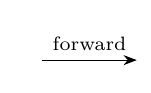
\begin{tikzpicture}[>=Stealth]
    \threebythree{3,-1,2,-2,1,-4,1,5,-3}{1,3,5,8}{}{ReLU input $z$}
    \draw[->] (1.8,-0.825) -- (3.0,-0.825) node[midway, above, font=\scriptsize] {forward};
    \begin{scope}[xshift=3.15cm]\threebythree{3,0,2,0,1,0,1,5,0}{}{}{output $\relu(z)$}\end{scope}
    \begin{scope}[xshift=6.6cm]\threebythree{1,-2,3,2,4,-1,-3,1,2}{}{1,5,6}{backward signal $g$}\end{scope}
    \begin{scope}[yshift=-2.6cm]
      \begin{scope}[xshift=0cm]\threebythree{1,0,3,0,4,0,-3,1,0}{1,3,5,8}{}{gradient}\end{scope}
      \begin{scope}[xshift=3.3cm]\threebythree{1,0,3,2,4,0,0,1,2}{}{1,5,6}{deconvnet}\end{scope}
      \begin{scope}[xshift=6.6cm]\threebythree{1,0,3,0,4,0,0,1,0}{1,3,5,8}{6}{guided backprop}\end{scope}
    \end{scope}
  \end{tikzpicture}
  \caption{The three ReLU rules on a $3\times 3$ layer. Top: the forward pass (red, $z<0$) and the backward signal arriving at the ReLU output (yellow, $g<0$). Bottom: the signal passed back to $z$. The gradient zeroes cells where the forward input was negative, the deconvnet zeroes cells where the backward signal is negative, and guided backpropagation zeroes both. Layout after \citet{springenberg2015}, with different numbers.}
  \label{fig:relu_rules}
\end{figure}

\subsection{Intuition: positive paths}

Guided backpropagation is a heuristic, but there is an intuitive argument for it~\citep{guerzhoy_video}. Since the network is linear apart from the ReLUs and max switches, the gradient with respect to an input is a sum over all paths from that input to the output of the product of the weights along the path, restricted to paths through active units. Some paths carry positive evidence and others negative evidence. Consider an image classifier that outputs the probability of ``cat'' (Figure~\ref{fig:positive_paths}). A pixel in the eye of a cat activates a ``cat eye'' unit, which is positive evidence for a cat. The same pixel may also feed, with a negative weight, into a ``dog ear'' unit that in turn provides evidence against a cat. The gradient adds the positive and negative paths, so that the pixel's importance is partly cancelled. Guided backpropagation only propagates signal along paths on which the backward signal stays positive. It therefore sums only positive evidence, which gives sparser maps in which the features that support the prediction stand out. The price is that it ignores negative evidence entirely.

\begin{figure}[t]
  \centering
  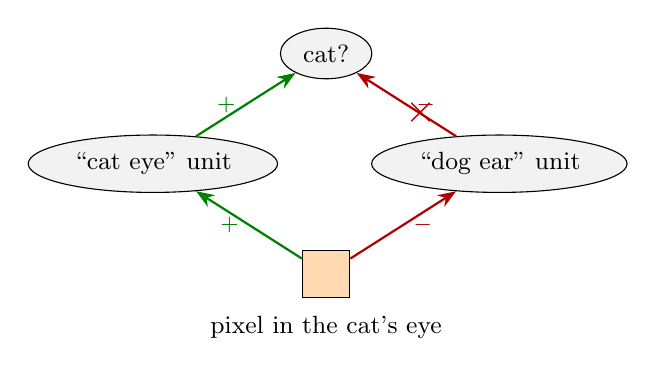
\begin{tikzpicture}[>=Stealth, every node/.style={font=\small}]
    \node[draw, ellipse, fill=gray!10] (cat) at (0,2.6) {cat?};
    \node[draw, ellipse, fill=gray!10] (eye) at (-2.2,1.2) {``cat eye'' unit};
    \node[draw, ellipse, fill=gray!10] (ear) at (2.2,1.2) {``dog ear'' unit};
    \node[draw, minimum size=6mm, fill=orange!30] (pix) at (0,-0.2) {};
    \node[below=1mm of pix] {pixel in the cat's eye};
    \draw[->, thick, green!50!black] (pix) -- node[left, font=\footnotesize] {$+$} (eye);
    \draw[->, thick, green!50!black] (eye) -- node[left, font=\footnotesize] {$+$} (cat);
    \draw[->, thick, red!70!black] (pix) -- node[right, font=\footnotesize] {$-$} (ear);
    \draw[->, thick, red!70!black] (ear) -- node[right, font=\footnotesize] {$-$} (cat);
    \node[red!70!black, font=\Large] at (1.2,1.85) {$\times$};
  \end{tikzpicture}
  \caption{Intuition for guided backpropagation. A pixel provides positive evidence for ``cat'' through a cat-eye detector (green path). The gradient also counts paths through other units, such as one through a dog-ear detector, which may carry signal of the opposite sign (red path). Guided backpropagation drops paths on which the backward signal becomes negative (cross). After an example by M.~Guerzhoy~\citep{guerzhoy_video}.}
  \label{fig:positive_paths}
\end{figure}

\subsection{Limitations}

These methods share several limitations.
\begin{itemize}
  \item They are defined for ReLUs (and max pooling). Modern networks use many other non-linearities, such as GELU, sigmoid and softmax, for which there is no obvious analogue of~\eqref{eq:relu_rules}.
  \item They ignore intercept terms, which, as we will see next, is part of why they fail on saturation and threshold effects.
  \item The deconvnet and guided backpropagation are not explanations of the model in any precise sense. Guided backpropagation in particular can produce plausible-looking maps that change little when the network's weights are randomized~\citep{adebayo2018}, because in deep image networks it largely reconstructs the input~\citep{nie2018}. Visual appeal is not evidence of faithfulness to the model.
\end{itemize}

\subsection{Saturation and thresholds revisited}
\label{sec:failure_modes}

Return to the saturating network~\eqref{eq:sat_net} at $\vx=(1,1)$. The backward signal at $h$ is the output weight, $\partial y/\partial h=-1$. The forward input to the ReLU is $z=-1<0$, so the gradient is zeroed; the deconvnet zeroes it because $-1<0$; and guided backpropagation zeroes it for both reasons. All three methods give scores $(0,0)$ for $x_1$ and $x_2$, the same failure as single-feature perturbation. The gradient describes the function at $\vx$, where it is flat, and says nothing about how the output got there.

\begin{figure}[t]
  \centering
  \newcommand{\thrnet}[9]{% inputs a,b,c ; za, ra ; zb, rb ; y ; title
    \node[nn] (a) at (0,0) {$#1$}; \node[nn] (b) at (1.4,0) {$#2$}; \node[nn] (c) at (2.8,0) {$#3$};
    \node[nn] (za) at (0,1.2) {$#4$}; \node[nn] (ra) at (0,2.2) {$#5$};
    \node[nn] (zb) at (2.1,1.2) {$#6$}; \node[nn] (rb) at (2.1,2.2) {$#7$};
    \node[nn] (y) at (1.05,3.3) {$#8$};
    \draw (a) -- node[wlab, left] {$1$} (za); \draw (za) -- (ra);
    \draw (b) -- node[wlab, left] {$1$} (zb); \draw (c) -- node[wlab, right] {$-1.5$} (zb); \draw (zb) -- (rb);
    \draw (ra) -- node[wlab, left] {$2$} (y); \draw (rb) -- node[wlab, right] {$2$} (y);
    \node[font=\footnotesize, below] at (a.south) {$a$}; \node[font=\footnotesize, below] at (b.south) {$b$};
    \node[font=\footnotesize, below] at (c.south) {$c$};
    \node[font=\small\bfseries, anchor=west] at (-0.5,4.0) {#9};}
  \begin{tikzpicture}[scale=0.9, every node/.append style={transform shape}]
    \thrnet{1}{2}{1}{1}{1}{0.5}{0.5}{3}{(a) forward}
    \node[lyr] at (-0.4,1.7) {ReLU};
    \begin{scope}[xshift=4.3cm]\thrnet{2}{2}{-3}{2}{2}{2}{2}{1}{(b) gradient}\end{scope}
    \begin{scope}[xshift=8.6cm]\thrnet{0}{0}{1}{0}{0}{-1.5}{0}{0}{(c) reference}\end{scope}
    \begin{scope}[xshift=12.9cm]\thrnet{2}{\frac12}{-\frac34}{2}{2}{\frac12}{2}{1}{(d) multipliers}\end{scope}
  \end{tikzpicture}
  \caption{The threshold failure mode. (a) A network with output $y=2\relu(a)+2\relu(b-1.5c)$ evaluated at $(a,b,c)=(1,2,1)$; the input $c$ acts as a fixed threshold. (b) Gradients: gradient $\times$ input gives $a$ a score of 2 and $b$ a score of 4, although the left branch contributes 2 to the output and the right branch only 1. (c) The reference input $(0,0,1)$, with output 0. (d) DeepLIFT multipliers $m_{\Delta u\Delta y}$ for each node $u$; contributions $m\,\Delta u$ are 2 for $a$, 1 for $b$ and 0 for $c$, summing to $\Delta y=3$ (Section~\ref{sec:deeplift}).}
  \label{fig:threshold}
\end{figure}

A second failure mode involves thresholds (Figure~\ref{fig:threshold}a). Consider three inputs $a,b,c$ and the network
\begin{equation}
  y = 2\,\relu(a) + 2\,\relu(b - 1.5\,c),
\end{equation}
where $c$ is held at 1, so that it acts as a threshold of 1.5 on $b$, like an intercept. At $(a,b,c)=(1,2,1)$, the left branch contributes $2\times 1=2$ to $y$ and the right branch $2\times 0.5=1$, so $y=3$. Both ReLUs are active, and the gradients are $\partial y/\partial a=2$, $\partial y/\partial b=2$ and $\partial y/\partial c=-3$ (Figure~\ref{fig:threshold}b). Gradient $\times$ input gives scores of $2\times1=2$ for $a$ and $2\times 2=4$ for $b$, ranking $b$ above $a$, although $a$ is responsible for more of the output. The gradient sees only the local slope of the right branch, not that most of $b$'s value is spent getting over the threshold.

%======================================================================
\section{DeepLIFT: differences from a reference}
\label{sec:deeplift}
%======================================================================

DeepLIFT~\citep{shrikumar2017} moves away from gradients. It explains the difference between the output for the input of interest and the output for a \emph{reference} input, and propagates these differences, rather than infinitesimal changes, back through the network. This solves the saturation and threshold problems, handles intercepts, and is defined for activation functions other than ReLU. It keeps the computational cost of a single backward pass.

\subsection{Contributions and multipliers}

Let $\vx^0\in\R^P$ be a reference input, with output $y^0=f(\vx^0)$. For every node $u$ of the network (an input, a hidden unit or the output) let $u^0$ be its value when the network is run on $\vx^0$, and $\Delta u=u-u^0$ its difference from reference. In particular $\Delta x_i=x_i-x^0_i$ and $\Delta y=y-y^0$. DeepLIFT assigns to each input a \emph{contribution} $C_{\Delta x_i\Delta y}\in\R$, the part of $\Delta y$ attributed to $\Delta x_i$, such that the contributions satisfy \emph{summation-to-delta},
\begin{equation}
  \sum_{i=1}^P C_{\Delta x_i\Delta y} = \Delta y .
  \label{eq:sum_to_delta}
\end{equation}
The \emph{multiplier} is the contribution per unit difference,
\begin{equation}
  m_{\Delta x_i\Delta y} = \frac{C_{\Delta x_i\Delta y}}{\Delta x_i}.
  \label{eq:multiplier}
\end{equation}
The multiplier is a finite-difference analogue of the partial derivative $\partial y/\partial x_i$, which is the limit of $\Delta y/\Delta x$ as $\Delta x\to 0$. In one dimension, the gradient is the slope of the tangent at $x$, while the multiplier is the slope of the secant from the reference $x^0$ to $x$ (Figure~\ref{fig:secant}). Where the function saturates, the tangent is flat but the secant is not.

\begin{figure}[t]
  \centering
  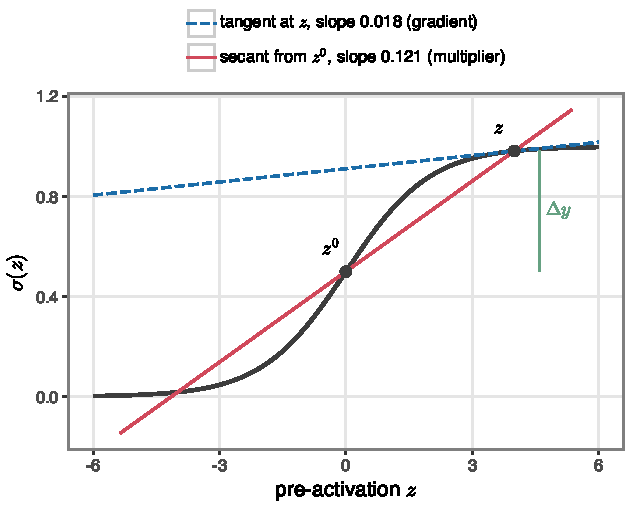
\includegraphics[width=0.55\linewidth]{secant.pdf}
  \caption{Gradient versus DeepLIFT multiplier for a sigmoid unit $\sigma(z)=1/(1+e^{-z})$, with reference $z^0=0$ (where $\sigma=0.5$) and input $z=4$. The gradient is the slope of the tangent at $z$ and is close to zero because the sigmoid has saturated. The multiplier is the slope of the secant from $z^0$ to $z$, $\Delta y/\Delta z$, and remains substantial. For $z\gg 0$ the difference from reference approaches $+0.5$.}
  \label{fig:secant}
\end{figure}

\subsection{The chain rule for multipliers}

Multipliers can be backpropagated in the same way as gradients. Recall the chain rule for gradients: if a parameter $w$ affects $y$ only through intermediate nodes $x_1,\dots,x_P$, then $\frac{\partial y}{\partial w}=\sum_i\frac{\partial x_i}{\partial w}\frac{\partial y}{\partial x_i}$. The analogous rule for multipliers is the following. Let $x_1,\dots,x_P$ be the inputs and $z_1,\dots,z_J$ a layer of nodes such that every path from the inputs to $y$ passes through exactly one $z_j$. Suppose we have multipliers $m_{\Delta x_i\Delta z_j}$ that satisfy summation-to-delta for each $z_j$, $\sum_i m_{\Delta x_i\Delta z_j}\Delta x_i=\Delta z_j$, and multipliers $m_{\Delta z_j\Delta y}$ that satisfy $\sum_j m_{\Delta z_j\Delta y}\Delta z_j=\Delta y$. Define
\begin{equation}
  m_{\Delta x_i\Delta y} = \sum_{j=1}^J m_{\Delta x_i\Delta z_j}\, m_{\Delta z_j\Delta y}.
  \label{eq:mult_chain}
\end{equation}
Then summation-to-delta holds for the composition, since
\begin{equation}
  \sum_{i=1}^P m_{\Delta x_i\Delta y}\Delta x_i
  = \sum_{j=1}^J m_{\Delta z_j\Delta y}\sum_{i=1}^P m_{\Delta x_i\Delta z_j}\Delta x_i
  = \sum_{j=1}^J m_{\Delta z_j\Delta y}\,\Delta z_j = \Delta y .
\end{equation}
Applying~\eqref{eq:mult_chain} layer by layer from the output down gives the multiplier of every node with respect to $y$ in one backward pass, after one forward pass on the input and one on the reference. We write $m_{\Delta u\Delta y}$ for the multiplier stored at node $u$, and $m_{\Delta u\Delta v}$ for the multiplier on an edge from $u$ to $v$, the analogue of $\partial v/\partial u$. Exactly as for gradients, the value at a node is the sum over its outgoing edges of the edge multiplier times the value at the node above.

\subsection{Rules for linear units and ReLUs}

We need local multipliers for each type of operation (Table~\ref{tab:mult_rules}).

\paragraph{Linear units.} For $z=b+\sum_i w_ix_i$ with intercept $b$, the reference value is $z^0=b+\sum_iw_ix_i^0$, so $\Delta z=\sum_i w_i\Delta x_i$: the intercept cancels. The natural contributions are $C_{\Delta x_i\Delta z}=w_i\Delta x_i$, which satisfy summation-to-delta, and the multipliers are $m_{\Delta x_i\Delta z}=w_i$, the same as the gradient.

\paragraph{ReLUs (the Rescale rule).} For $h=\relu(z)$, with a single input, summation-to-delta forces $C_{\Delta z\Delta h}=\Delta h$, so
\begin{equation}
  m_{\Delta z\Delta h} = \frac{\Delta h}{\Delta z} = \frac{\relu(z)-\relu(z^0)}{z-z^0}.
  \label{eq:rescale}
\end{equation}
When $\Delta z=0$ we also have $\Delta h=0$, and the multiplier is set to the gradient, its limit as $\Delta z\to 0$. The same rule applies to any elementwise non-linearity $h=\sigma(z)$, such as a sigmoid, tanh or GELU, by replacing $\relu$ with $\sigma$ in~\eqref{eq:rescale}. Unlike the gradient, the multiplier depends on the reference value $z^0$ as well as on $z$. \citet{shrikumar2017} also propose a ``RevealCancel'' rule, which treats positive and negative contributions to $\Delta z$ separately; we use only Rescale here.

\begin{table}[t]
  \centering
  \caption{Gradients and DeepLIFT multipliers for the two operations of a ReLU network. $\ind[\cdot]$ is the indicator function and $\Delta$ denotes the difference from the reference.}
  \label{tab:mult_rules}
  \begin{tabular}{lll}
    \toprule
    Function & Gradient & Multiplier \\
    \midrule
    $z=b+\sum_iw_ix_i$ & $\partial z/\partial x_i = w_i$ & $C_{\Delta x_i\Delta z}=w_i\Delta x_i$, \quad $m_{\Delta x_i\Delta z}=w_i$ \\[2pt]
    $h=\max(0,z)$ & $\partial h/\partial z=\ind[z>0]$ & $C_{\Delta z\Delta h}=\Delta h$, \quad $m_{\Delta z\Delta h}=\Delta h/\Delta z$ \\
    \bottomrule
  \end{tabular}
\end{table}

\subsection{Saturation and thresholds with DeepLIFT}

\begin{figure}[t]
  \centering
  \newcommand{\satnet}[6]{% x1, x2, z, h, y, title
    \node[nn] (x1) at (0,0) {$#1$}; \node[nn] (x2) at (1.4,0) {$#2$};
    \node[nn] (z) at (0.7,1.2) {$#3$}; \node[nn] (h) at (0.7,2.1) {$#4$}; \node[nn] (y) at (0.7,3.1) {$#5$};
    \node[nnb, right=1mm of z] {$+1$}; \node[nnb, right=1mm of y] {$+1$};
    \draw (x1) -- node[wlab, left] {$-1$} (z); \draw (x2) -- node[wlab, right] {$-1$} (z);
    \draw (z) -- (h); \draw (h) -- node[wlab, left] {$-1$} (y);
    \node[font=\footnotesize, below] at (x1.south) {$x_1$}; \node[font=\footnotesize, below] at (x2.south) {$x_2$};
    \node[font=\small\bfseries, anchor=west] at (-0.5,3.8) {#6};}
  \begin{tikzpicture}
    \satnet{1}{1}{-1}{0}{1}{(a) input}
    \node[lyr] at (0.35,1.65) {ReLU};
    \begin{scope}[xshift=3.6cm]\satnet{0}{0}{1}{1}{0}{(b) reference}\end{scope}
    \begin{scope}[xshift=7.2cm]\satnet{\frac12}{\frac12}{-\frac12}{-1}{1}{(c) multipliers}
      \node[font=\scriptsize, right] at (1.45,1.65) {$\dfrac{\Delta h}{\Delta z}=\dfrac{0-1}{-1-1}=\dfrac12$};
      \node[font=\footnotesize, below=0.35cm] at (x1.south) {$C=\frac12$};
      \node[font=\footnotesize, below=0.35cm] at (x2.south) {$C=\frac12$};
    \end{scope}
  \end{tikzpicture}
  \caption{DeepLIFT on the saturating network of Figure~\ref{fig:saturation}. (a) Forward pass on the input $(1,1)$. (b) Forward pass on the reference $(0,0)$. (c) Backward pass of multipliers $m_{\Delta u\Delta y}$, starting from 1 at the output. The ReLU multiplier is $\Delta h/\Delta z=\frac12$, so each input receives multiplier $\frac12$ and contribution $C=m\,\Delta x=\frac12$; the contributions sum to $\Delta y=1$.}
  \label{fig:deeplift_sat}
\end{figure}

For the saturating network~\eqref{eq:sat_net}, take the reference $\vx^0=(0,0)$ (Figure~\ref{fig:deeplift_sat}). On the reference, $z^0=1$, $h^0=1$ and $y^0=0$; on the input $(1,1)$, $z=-1$, $h=0$ and $y=1$, so $\Delta y=1$. Backpropagating multipliers: the output node has multiplier 1; the edge from $h$ to $y$ is linear with weight $-1$, so $m_{\Delta h\Delta y}=-1$. The ReLU multiplier is $\Delta h/\Delta z=(0-1)/(-1-1)=\frac12$, where the gradient would be 0, so $m_{\Delta z\Delta y}=-1\times\frac12=-\frac12$. Each input edge has weight $-1$, so $m_{\Delta x_1\Delta y}=m_{\Delta x_2\Delta y}=\frac12$, and the contributions are $C_{\Delta x_i\Delta y}=\frac12\times 1=\frac12$. Both inputs receive equal credit, and the contributions sum to $\Delta y=1$. The gradient was zero because the output is flat at $\vx$; the multiplier sees the whole change from the reference.

For the threshold network (Figure~\ref{fig:threshold}c,d), take the reference $(a,b,c)=(0,0,1)$, which keeps the threshold input $c$ at its value. The reference output is $y^0=2\relu(0)+2\relu(-1.5)=0$, so $\Delta y=3$. In the left branch, the ReLU multiplier is $(1-0)/(1-0)=1$, so $m_{\Delta a\Delta y}=2$ and $C_{\Delta a\Delta y}=2\times 1=2$. In the right branch, the pre-activation goes from $-1.5$ to $0.5$ and the activation from $0$ to $0.5$, so the ReLU multiplier is $0.5/2=\frac14$, $m_{\Delta b\Delta y}=2\times\frac14\times 1=\frac12$ and $C_{\Delta b\Delta y}=\frac12\times 2=1$. Since $\Delta c=0$, $C_{\Delta c\Delta y}=0$. DeepLIFT therefore assigns 2 to $a$ and 1 to $b$, matching the amounts each branch adds to the output, where gradient $\times$ input gave 2 and 4.

\subsection{A worked example}
\label{sec:deeplift_example}

Consider a network with four inputs $\vx\in\R^4$, three hidden ReLU units with intercepts, and a linear output with no intercept,
\begin{equation}
  \begin{aligned}
    z_1 &= 2x_1 + x_2 - 1, & z_2 &= -x_2 + x_3, & z_3 &= -2x_3 + 2x_4 + 2,\\
    y &= -\relu(z_1) + 2\relu(z_2) + \relu(z_3). & & & &
  \end{aligned}
  \label{eq:ex1_net}
\end{equation}
At the input $\vx=(1,2,0,1)$ the pre-activations are $\vz=(3,-2,4)$, the activations $\vh=(3,0,4)$ and the output $y=-3+0+4=1$. At the reference $\vx^0=\mathbf{0}$ they are $\vz^0=(-1,0,2)$, $\vh^0=(0,0,2)$ and $y^0=2$, so $\Delta y=-1$. The multipliers of the activations are the output weights, $(-1,2,1)$. The ReLU multipliers are
\begin{equation}
  \frac{\Delta h_1}{\Delta z_1}=\frac{3-0}{3-(-1)}=\frac34, \qquad
  \frac{\Delta h_2}{\Delta z_2}=\frac{0-0}{-2-0}=0, \qquad
  \frac{\Delta h_3}{\Delta z_3}=\frac{4-2}{4-2}=1,
\end{equation}
so the multipliers of the pre-activations are $(-1\times\frac34,\;2\times 0,\;1\times 1)=(-\frac34,0,1)$. Each input multiplier is the sum over its outgoing edges of weight times the multiplier above, for example $m_{\Delta x_2\Delta y}=1\times(-\frac34)+(-1)\times 0=-\frac34$. Table~\ref{tab:deeplift_example} collects the results and compares them with the gradient. The DeepLIFT contributions sum to $\Delta y=-1$; gradient $\times$ input sums to $-2$, because the gradient ignores the intercepts and the change in the third ReLU's operating point between reference and input.

\begin{table}[t]
  \centering
  \caption{Gradient and DeepLIFT for the network~\eqref{eq:ex1_net} at $\vx=(1,2,0,1)$ with reference $\vx^0=\mathbf{0}$. The DeepLIFT contributions sum to $\Delta y=y-y^0=1-2=-1$.}
  \label{tab:deeplift_example}
  \begin{tabular}{crrrrr}
    \toprule
    Input & $\Delta x_i$ & $\partial y/\partial x_i$ & $x_i\,\partial y/\partial x_i$ & $m_{\Delta x_i\Delta y}$ & $C_{\Delta x_i\Delta y}$ \\
    \midrule
    $x_1$ & 1 & $-2$ & $-2$ & $-\frac32$ & $-\frac32$ \\[1pt]
    $x_2$ & 2 & $-1$ & $-2$ & $-\frac34$ & $-\frac32$ \\[1pt]
    $x_3$ & 0 & $-2$ & 0 & $-2$ & 0 \\
    $x_4$ & 1 & 2 & 2 & 2 & 2 \\
    \midrule
    sum & & & $-2$ & & $-1$ \\
    \bottomrule
  \end{tabular}
\end{table}

\subsection{Relation to gradient times input}

If every intercept in a ReLU network is zero and the reference is $\vx^0=\mathbf{0}$, then every node has reference value zero. For a ReLU with $z>0$ the Rescale multiplier is $(z-0)/(z-0)=1$, and with $z<0$ it is $(0-0)/(z-0)=0$; both equal the gradient $\ind[z>0]$. Linear multipliers always equal the weights. Hence every multiplier equals the corresponding partial derivative, and the DeepLIFT contributions are $C_{\Delta x_i\Delta y}=x_i\,\partial y/\partial x_i$, gradient $\times$ input~\citep{shrikumar2017,ancona2018}. In this case gradient $\times$ input also sums to $y-y^0=y$: such a network is positively homogeneous, $f(\lambda\vx)=\lambda f(\vx)$ for $\lambda>0$, and differentiating with respect to $\lambda$ at $\lambda=1$ gives Euler's identity $\sum_i x_i\,\partial f/\partial x_i=f(\vx)$. The differences between the methods arise from the intercepts and from non-zero references, which is where gradient $\times$ input goes wrong in the examples above.

\subsection{Choosing the reference}

DeepLIFT scores answer the question ``important relative to what?'', and the answer depends on the reference. For images an all-black image is a common choice. For one-hot DNA, options include the all-zero input (no base at any position), the expected one-hot vector under background base frequencies (for example $0.25$ for each base), and shuffled versions of the input sequence that preserve its dinucleotide composition, with contributions averaged over several shuffles. A reference should be uninformative for the prediction, so that $\Delta y$ reflects the signal in the input. Figure~\ref{fig:secant} shows a related subtlety for sigmoid units: with reference pre-activation 0 the reference activation is $0.5$, not 0, and the difference from reference can be at most $0.5$ in either direction.

%======================================================================
\section{Integrated gradients}
\label{sec:ig}
%======================================================================

Integrated gradients~\citep{sundararajan2017} also explain $f(\vx)-f(\vx^0)$ relative to a reference (called the baseline), but use only gradients of $f$, with no special backpropagation rules. The idea is to average the gradient along the straight path from the reference to the input. Let $\boldsymbol{\gamma}(\alpha)=\vx^0+\alpha(\vx-\vx^0)$ for $\alpha\in[0,1]$. The integrated gradient of feature $i$ is
\begin{equation}
  \IG_i(\vx) = (x_i-x_i^0)\int_0^1 \frac{\partial f}{\partial x_i}\big(\boldsymbol{\gamma}(\alpha)\big)\,d\alpha .
  \label{eq:ig}
\end{equation}
Integrated gradients satisfy summation-to-delta, which \citet{sundararajan2017} call \emph{completeness}. By the fundamental theorem of calculus and the chain rule,
\begin{equation}
  f(\vx)-f(\vx^0) = \int_0^1 \frac{d}{d\alpha}f\big(\boldsymbol{\gamma}(\alpha)\big)\,d\alpha
  = \int_0^1 \sum_{i=1}^P \frac{\partial f}{\partial x_i}\big(\boldsymbol{\gamma}(\alpha)\big)\,(x_i-x_i^0)\,d\alpha
  = \sum_{i=1}^P \IG_i(\vx),
\end{equation}
using $d\gamma_i/d\alpha=x_i-x_i^0$. This requires $f$ to be differentiable almost everywhere along the path, which holds for ReLU networks.

\paragraph{The saturation example.} For $y=\min(x_1+x_2,1)$ with $\vx=(1,1)$ and $\vx^0=(0,0)$, the path is $\boldsymbol{\gamma}(\alpha)=(\alpha,\alpha)$, on which $y=\min(2\alpha,1)$. The gradient $\partial y/\partial x_1$ is 1 for $\alpha<\frac12$, before the function saturates, and 0 afterwards (Figure~\ref{fig:ig_sat}). The integral is $\frac12$, so $\IG_1=\IG_2=(1-0)\times\frac12=\frac12$, the same as DeepLIFT. For the threshold example, the gradient with respect to $a$ is 2 along the whole path, giving $\IG_a=2$. The right ReLU becomes active when $2\alpha-1.5>0$, that is for $\alpha>\frac34$, so $\IG_b=2\times\int_{3/4}^1 2\,d\alpha=1$, again matching DeepLIFT.

\begin{figure}[t]
  \centering
  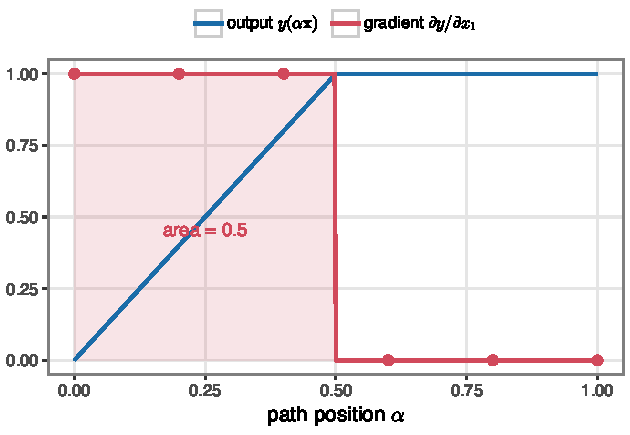
\includegraphics[width=0.6\linewidth]{ig_saturation.pdf}
  \caption{Integrated gradients for $y=\min(x_1+x_2,1)$ along the path $\alpha\vx$ from the reference $(0,0)$ to $\vx=(1,1)$. The output (blue) rises until $\alpha=\frac12$ and then saturates, and the gradient with respect to $x_1$ (red) drops to zero. Its integral, the shaded area, is $\frac12$, so each input receives $\IG_i=\frac12$. Points mark a six-point Riemann approximation at $\alpha=0,0.2,\dots,1$, whose average is also $\frac12$.}
  \label{fig:ig_sat}
\end{figure}

\paragraph{Computation.} In practice the integral is approximated by a Riemann sum over $K$ points on the path (Algorithm~\ref{alg:ig}), typically with $K$ between 20 and 300, which costs $K$ gradient evaluations. In the saturation example, the gradient at $\alpha=0,0.2,0.4$ is 1 and at $\alpha=0.6,0.8,1$ is 0, whose average is $\frac12$, giving the same answer.

\begin{algorithm}[t]
  \caption{Integrated gradients with a midpoint Riemann sum}
  \label{alg:ig}
  \begin{algorithmic}[1]
    \Require model $f$, input $\vx$, reference $\vx^0$, number of steps $K$
    \State $\vg\gets\mathbf{0}\in\R^P$
    \For{$k=1,\dots,K$}
      \State $\alpha\gets (k-\frac12)/K$
      \State $\vg\gets\vg+\nabla_{\vx}f\big(\vx^0+\alpha(\vx-\vx^0)\big)$ \Comment{one forward and one backward pass}
    \EndFor
    \State \Return $(\vx-\vx^0)\odot\vg/K$ \Comment{$\odot$: elementwise product}
  \end{algorithmic}
\end{algorithm}

\paragraph{Pros and cons.} Integrated gradients treat the model as a black box apart from requiring its gradients, so they apply to any differentiable architecture. Because they depend only on the function $f$, two networks that compute the same function are guaranteed to receive the same attributions, a property called \emph{implementation invariance}. DeepLIFT's rules, in contrast, are applied to the network's computation graph, and two implementations of the same function can receive different DeepLIFT scores. The cost is the $K$ repeated gradient calculations, compared with one backward pass for DeepLIFT.

\paragraph{Expected gradients.} The choice of reference matters for integrated gradients as it does for DeepLIFT. \emph{Expected gradients}~\citep{erion2021} average integrated gradients over references drawn from the data, $\vx^0\sim\mathcal{D}$, and over the path position $\alpha\sim\mathrm{Uniform}(0,1)$,
\begin{equation}
  \mathrm{EG}_i(\vx) = \E_{\vx^0\sim\mathcal{D},\,\alpha\sim U(0,1)}\left[(x_i-x_i^0)\,\frac{\partial f}{\partial x_i}\big(\vx^0+\alpha(\vx-\vx^0)\big)\right],
\end{equation}
which is estimated by sampling pairs $(\vx^0,\alpha)$. This removes the need to pick a single reference and fits naturally into training with stochastic gradients.

%======================================================================
\section{Shapley values and SHAP}
\label{sec:shap}
%======================================================================

DeepLIFT and integrated gradients both distribute $f(\vx)-f(\vx^0)$ among the input features, but by different rules. Is there a principled way to choose among such rules? \citet{lundberg2017} showed that a small set of desirable properties singles out one attribution, based on the Shapley value from cooperative game theory~\citep{shapley1953}, and that several existing methods, DeepLIFT among them, can be viewed as approximations to it.

\subsection{Additive feature attribution}

Let $y=f(\vx)$ be the trained model. The goal is to find a simple explanation model $g\approx f$ that is valid near $\vx$. Explanations are defined on a \emph{simplified} binary input $\vx'\in\{0,1\}^P$ indicating which features are ``present'', together with a mapping $h_{\vx}$ back to the original input space. For DeepLIFT-style explanations, an absent feature takes its reference value,
\begin{equation}
  h_{\vx}(\vz')_i = \begin{cases} x_i^0 & \text{if } z'_i=0,\\ x_i & \text{if } z'_i=1,\end{cases}
\end{equation}
for $\vz'\in\{0,1\}^P$, so that $h_{\vx}(\mathbf{1})=\vx$ and $h_{\vx}(\mathbf{0})=\vx^0$. The input itself corresponds to $\vx'=\mathbf{1}$. An \emph{additive feature attribution} method uses an explanation model that is linear in the simplified inputs,
\begin{equation}
  g(\vz') = \phi_0 + \sum_{i=1}^P\phi_i z'_i ,
  \label{eq:additive}
\end{equation}
for $\vz'$ ``near'' $\vx'$, meaning $\vz'\subseteq\vx'$: $\vz'$ can only switch off features that are present in $\vx'$. Here $\phi_i\in\R$ is the attribution of feature $i$ and $\phi_0$ a constant. DeepLIFT is of this form, with $\phi_0=f(\vx^0)$ and $\phi_i=C_{\Delta x_i\Delta y}$, and so are integrated gradients, LIME and others.

\subsection{Three properties}

Write $f_{\vx}(\vz')=f(h_{\vx}(\vz'))$ for the model evaluated with only the features in $\vz'$ present, and $\vz'\setminus i$ for $\vz'$ with $z'_i$ set to zero. \citet{lundberg2017} ask for three properties.
\begin{enumerate}
  \item \emph{Local accuracy.} The explanation matches the model at the input: $f(\vx)=g(\vx')=\phi_0+\sum_i\phi_i x'_i$. With $\vx'=\mathbf{1}$ and $\phi_0=f(\vx^0)$ this is summation-to-delta.
  \item \emph{Missingness.} A feature that is absent gets no attribution: $x'_i=0\Rightarrow\phi_i=0$.
  \item \emph{Consistency.} If a model changes so that feature $i$'s marginal contribution never decreases, its attribution should not decrease. Formally, for two models $f$ and $\tilde f$, if
  \begin{equation}
    \tilde f_{\vx}(\vz')-\tilde f_{\vx}(\vz'\setminus i) \geq f_{\vx}(\vz')-f_{\vx}(\vz'\setminus i) \quad\text{for all } \vz'\in\{0,1\}^P,
  \end{equation}
  then $\phi_i(\tilde f,\vx)\geq\phi_i(f,\vx)$.
\end{enumerate}

\subsection{The Shapley value}

The theorem of \citet{lundberg2017}, building on classical results for the Shapley value, is that exactly one additive feature attribution satisfies all three properties. Treating the features as players in a cooperative game whose payoff for a coalition $S\subseteq\{1,\dots,P\}$ of present features is $f_{\vx}(S)$ (the model with features in $S$ at their input values and the rest at the reference), the attributions are the Shapley values
\begin{equation}
  \phi_i = \sum_{S\subseteq\{1,\dots,P\}\setminus\{i\}} \frac{|S|!\,(P-|S|-1)!}{P!}\Big[f_{\vx}(S\cup\{i\})-f_{\vx}(S)\Big].
  \label{eq:shapley}
\end{equation}
The bracket is the marginal contribution of feature $i$ when it is added to the features in $S$: how important $i$ is when the features in $S$ are on. The weight can be written $\frac{1}{P}\binom{P-1}{|S|}^{-1}$: it averages first over the $P$ possible sizes of $S$ and then over all subsets of a given size. Equivalently, $\phi_i$ is the average, over all $P!$ orderings in which the features could be switched on one at a time starting from the reference, of the change in output when feature $i$ is switched on.

For the saturation example with reference $\mathbf{0}$, $f_{\vx}(\emptyset)=0$ and $f_{\vx}(\{1\})=f_{\vx}(\{2\})=f_{\vx}(\{1,2\})=1$, so
\begin{equation}
  \phi_1 = \tfrac12\big[f_{\vx}(\{1\})-f_{\vx}(\emptyset)\big]+\tfrac12\big[f_{\vx}(\{1,2\})-f_{\vx}(\{2\})\big] = \tfrac12(1-0)+\tfrac12(1-1) = \tfrac12,
\end{equation}
and by symmetry $\phi_2=\frac12$. For the threshold example (treating $c$ as fixed), $f_{\vx}(\emptyset)=0$, $f_{\vx}(\{a\})=2$, $f_{\vx}(\{b\})=1$ and $f_{\vx}(\{a,b\})=3$, giving $\phi_a=\frac12(2+2)=2$ and $\phi_b=\frac12(1+1)=1$. In both examples the Shapley values coincide with the DeepLIFT and integrated gradients attributions. For a linear model $f(\vx)=b+\vw^\top\vx$ all three methods give $\phi_i=w_i(x_i-x_i^0)$. In general they differ (Exercise 5).

\subsection{Approximating Shapley values}

The sum~\eqref{eq:shapley} has $2^{P-1}$ terms for each feature, which is infeasible for a sequence model with $P=4L$ inputs. There are two broad options.
\begin{enumerate}
  \item \emph{Sampling.} Estimate~\eqref{eq:shapley} by Monte Carlo, sampling orderings or subsets $S$. KernelSHAP~\citep{lundberg2017} is a model-agnostic variant that fits the additive model~\eqref{eq:additive} by weighted linear regression to the model's outputs on sampled coalitions, with weights chosen so that the solution recovers the Shapley values. This resembles LIME with a particular choice of weights.
  \item \emph{Exploiting the structure of $f$.} For a linear model the Shapley values are available in closed form, and DeepLIFT's rules can be viewed as composing exact attributions of simple components through the chain rule~\eqref{eq:mult_chain}. DeepSHAP~\citep{lundberg2017} uses this view, running DeepLIFT with multipliers averaged over a distribution of references, and gives a fast approximation to Shapley values for deep networks.
\end{enumerate}
The SHAP framework thus provides a theoretical motivation for DeepLIFT-style methods: they are cheap approximations to the unique attribution that satisfies local accuracy, missingness and consistency.

%======================================================================
\section{Example: motifs in simulated regulatory sequence}
\label{sec:sim_example}
%======================================================================

To compare the methods on a problem where the ground truth is known, we follow the design of a simulation used to motivate DeepLIFT~\citep{shrikumar2017}. Random DNA sequences of length $L=200$ are generated with each base drawn uniformly. Two motifs are inserted at random non-overlapping positions: a GATA motif (consensus \texttt{AGATAAG}) and a TAL1-like E-box motif (consensus \texttt{AACAGATGGT}), each base matching the consensus with probability 0.95. A sequence is positive if it contains \emph{both} motifs; negatives contain only the GATA motif, only the TAL1 motif or neither, in equal proportions, so the model must learn an AND of the two motifs. We trained a small CNN on 10,000 sequences: one convolutional layer with 16 filters of width 11, a ReLU, global average pooling, a dense layer of 16 ReLU units and a single output logit. It reached an AUROC of 0.97 on 1,000 held-out sequences.

Figure~\ref{fig:seq_attr} shows six attribution maps for one correctly predicted positive sequence. DeepLIFT and integrated gradients use the reference that has probability $0.25$ for every base at every position. The observations are typical of what is seen in practice.
\begin{itemize}
  \item ISM, with 600 forward passes, gives a clean map: mutating any base in either motif lowers the prediction, and background positions have little effect.
  \item Gradient $\times$ input highlights both motifs, but its scores are noisier, include positions outside the motifs, and contain a large negative score inside the TAL1 motif.
  \item Guided backpropagation is almost identical to the gradient for this model. With global average pooling, the backward signal reaching each convolutional filter is the same at every position, and for the filters that are active here it is already positive, so the guided rule rarely zeroes anything.
  \item The deconvnet fails completely: it ignores whether each filter was active at each position, and so returns essentially the same combination of filter weights at every position, independent of where the motifs are. This illustrates the warning of Section~\ref{sec:modified_backprop} that modified backpropagation rules need not explain the model.
  \item DeepLIFT and integrated gradients closely resemble ISM. The DeepLIFT contributions sum exactly to the difference in logits between input and reference, $8.65$; integrated gradients with 500 steps sum to $8.74$, within 1\% of it, the residual being Riemann approximation error; gradient $\times$ input sums to $5.94$.
\end{itemize}

\begin{figure}[p]
  \centering
  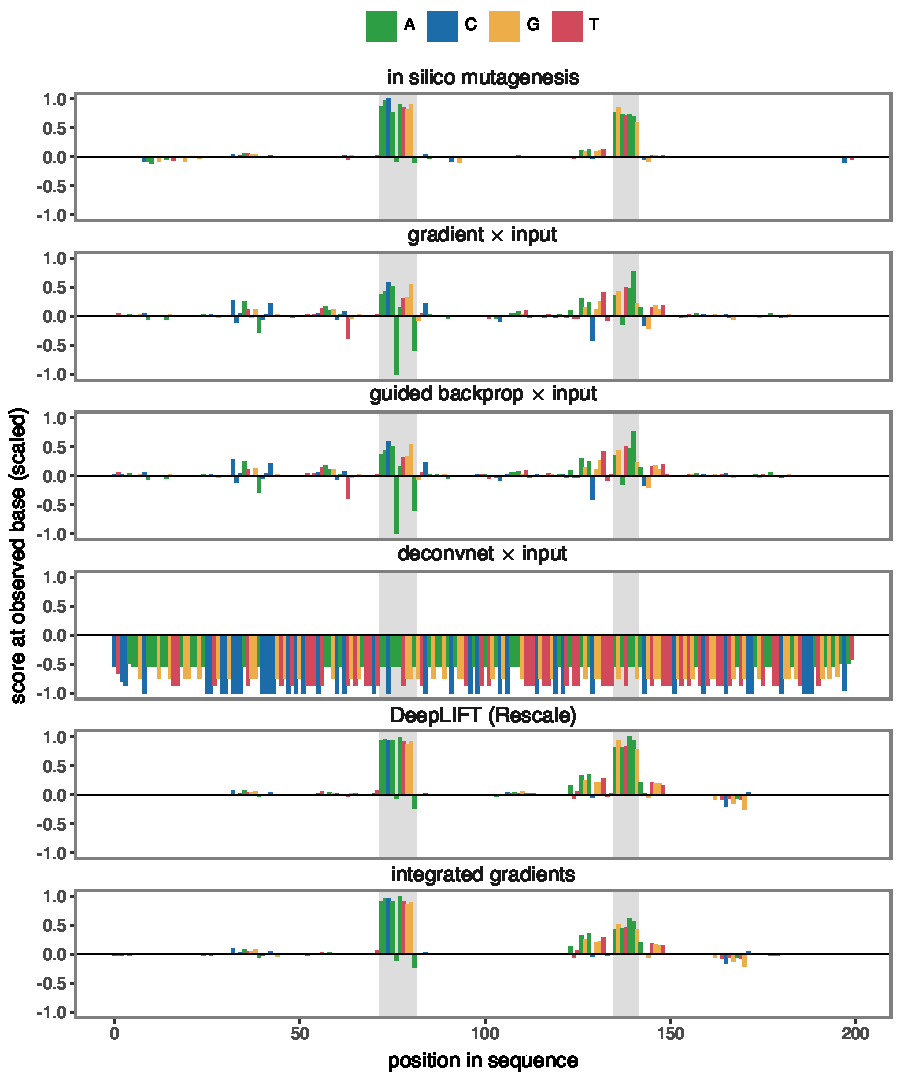
\includegraphics[width=0.8\linewidth]{sequence_attributions.pdf}
  \caption{Attribution maps for a simulated positive sequence containing a TAL1-like motif (grey band at positions 72--81) and a GATA motif (grey band at 135--141), for a CNN trained to detect sequences containing both motifs. Each bar is the score of the observed base at that position, coloured by base and scaled so that the largest absolute score in each panel is 1. ISM is the mean decrease in the logit over the three possible mutations. DeepLIFT and integrated gradients use a uniform reference (probability 0.25 for each base) and are summed over the four bases at each position. Simulated data; see \texttt{scripts/make\_figures.py}.}
  \label{fig:seq_attr}
\end{figure}

For real genomic models, attribution maps computed for many sequences are the starting point for further analysis. High-scoring subsequences can be clustered to discover motifs, positions with large attributions can be compared with experimentally measured effects of mutations, and the effects of genetic variants can be predicted with ISM or approximated with gradients or DeepLIFT (Chapter 3).

%======================================================================
\section{Summary}
%======================================================================

\begin{itemize}
  \item Interpretation methods assign importance scores to input features, usually for one prediction at a time. For sequence models, the scores show which nucleotides drive a prediction and often reveal transcription factor motifs.
  \item In silico mutagenesis perturbs each feature and reruns the model. It is simple and directly predicts the effects of mutations, but it needs one forward pass per perturbation and misses features that matter only in combination (saturation).
  \item Backpropagation gives the gradient of the output with respect to every input in one backward pass, a local linear approximation of the model. Guided backpropagation and deconvnets change the ReLU rule to give cleaner maps, but are heuristics and share the gradient's failures on saturation and thresholds.
  \item DeepLIFT and integrated gradients explain the difference in output from a reference input and satisfy summation-to-delta (completeness), which solves the saturation problem. DeepLIFT backpropagates multipliers $\Delta\text{out}/\Delta\text{in}$ in one pass; integrated gradients average gradients along a path at the cost of many passes but depend only on the function.
  \item Shapley values are the unique additive attribution with local accuracy, missingness and consistency. They are exponentially expensive to compute exactly, and SHAP provides a framework in which DeepLIFT-type methods are fast approximations.
\end{itemize}

%======================================================================
\section*{Exercises}
%======================================================================

\begin{enumerate}
  \item The toy network of Figure~\ref{fig:toycnn} is changed in two ways: the first layer becomes $z^{(1)}_1=-x_1+2x_2$, $z^{(1)}_2=x_2+x_3$, $z^{(1)}_3=-x_3+3x_4$, $z^{(1)}_4=-3x_4+4x_5$, and the final max is replaced by the linear output $y=2h^{(2)}_1-h^{(2)}_2$; $\mW^{(2)}$ is unchanged. For the input $\vx=(0,2,1,0,3)$, compute the forward pass and the input scores given by the gradient, the deconvnet and guided backpropagation, and the corresponding saliency maps (scores $\times$ input). \emph{(Answer: $y=2$; gradient $(-2,2,-2,0,0)$; deconvnet and guided backpropagation both $(-2,4,0,0,0)$.)}
  \item A network has inputs $\vx\in\R^4$, pre-activations $z_1=x_1-x_2+2$, $z_2=2x_2+x_3-2$, $z_3=x_3-3x_4$, ReLU activations $h_j=\relu(z_j)$ and output $y=h_1-2h_2+2h_3$. For the input $\vx=(0,1,2,1)$ and reference $\vx^0=\mathbf{0}$, run the forward pass on both, label every node with its DeepLIFT multiplier, and compute the contributions of the four inputs. Check that they sum to $\Delta y$. \emph{(Answer: contributions $(0,-3,-2,0)$, $\Delta y=-3-2=-5$.)} Compare with gradient $\times$ input.
  \item Show that for a linear model $f(\vx)=b+\vw^\top\vx$, gradient $\times$ input (with $\vx-\vx^0$ in place of $\vx$), DeepLIFT, integrated gradients and Shapley values all give $\phi_i=w_i(x_i-x_i^0)$.
  \item Show that for a single unit $y=\sigma(\vw^\top\vx+b)$, where $\sigma$ is any differentiable non-linearity, the DeepLIFT Rescale contributions equal $w_i\Delta x_i\,\Delta y/\Delta z$ with $z=\vw^\top\vx+b$. Show that integrated gradients give the same attributions. (Hint: along the straight path, $z$ changes linearly in $\alpha$.)
  \item Consider $y=\relu(x_1+x_2-1)$ with reference $\mathbf{0}$ and input $\vx=(2,0.5)$. Compute the DeepLIFT, integrated gradients and Shapley attributions. \emph{(Answer: DeepLIFT and integrated gradients give $(1.2,0.3)$; Shapley values are $(1.25,0.25)$.)} Which do you find more reasonable, and why?
  \item Show that the gradient $\times$ input of a ReLU network with zero intercepts sums to $f(\vx)$. Give an example of a network with non-zero intercepts for which it does not sum to $f(\vx)-f(\mathbf{0})$.
  \item Using a trained sequence model, for example the simulation of Section~\ref{sec:sim_example}, compare ISM with the first-order approximation~\eqref{eq:ism_approx} across all positions and alternative bases. Where is the approximation worst?
\end{enumerate}

\bibliographystyle{abbrvnat}
\bibliography{../chapter04/chapter04}
\endgroup

% Generated wrapper: chapter 05 with its own figure path, macros and bibliography.
\graphicspath{{../chapter05/figures/}}
\makeatletter\def\input@path{{../chapter05/}}\makeatother
\begingroup
% Chapter 5: unsupervised learning and clustering.
% Requires: amsmath, amssymb, bm, graphicx, booktabs, subcaption, algorithm, algpseudocode,
% tikz (arrows.meta, positioning, calc, decorations.pathreplacing, fit), natbib.
% Computed figures are produced by scripts/make_figures.py; figures/slides/ holds figures taken from the lecture slides.

\providecommand{\R}{\mathbb{R}}
\providecommand{\E}{\mathbb{E}}
\providecommand{\Normal}{\mathcal{N}}
\providecommand{\argmax}{\operatorname*{arg\,max}}
\providecommand{\argmin}{\operatorname*{arg\,min}}
\providecommand{\vy}{\mathbf{y}}
\providecommand{\vx}{\mathbf{x}}
\providecommand{\mX}{\mathbf{X}}
\providecommand{\mI}{\mathbf{I}}
\providecommand{\vb}{\boldsymbol{\beta}}
\providecommand{\veps}{\boldsymbol{\epsilon}}
\providecommand{\vp}{\mathbf{p}}
\providecommand{\vg}{\mathbf{g}}
\providecommand{\ind}{\mathbf{1}}
\providecommand{\vmu}{\boldsymbol{\mu}}
\providecommand{\vpi}{\boldsymbol{\pi}}
\providecommand{\vc}{\mathbf{c}}
\providecommand{\vf}{\mathbf{f}}
\providecommand{\vu}{\mathbf{u}}
\providecommand{\mSigma}{\boldsymbol{\Sigma}}
\providecommand{\mA}{\mathbf{A}}
\providecommand{\mD}{\mathbf{D}}
\providecommand{\mL}{\mathbf{L}}
\providecommand{\mU}{\mathbf{U}}
\providecommand{\mLambda}{\boldsymbol{\Lambda}}
\providecommand{\KL}{\operatorname{KL}}

\chapter{Unsupervised learning and clustering}
\label{ch:clustering}

The models in the earlier chapters were all supervised: each training example came with a label or response $y$, and the task was to predict it from the features $\vx$. Much of functional genomics data comes without labels. A single-cell RNA-seq experiment measures the expression of thousands of genes in each of thousands of cells, but nobody tells us which cell is a T cell and which is a monocyte. A cohort of tumour or post-mortem brain samples may contain molecular subtypes of disease that have never been described. This chapter introduces unsupervised learning, the problem of finding structure in $\mX$ alone, through its simplest and most widely used instance, clustering. We develop the Gaussian mixture model, derive the K-means algorithm as a way of fitting it, and then derive the expectation-maximization (EM) algorithm, which gives a ``soft'' version of K-means and recurs throughout the rest of the book. We then cover the clustering methods most used for single-cell data, hierarchical, spectral and graph-based clustering, and finish with the question of whether the clusters we find are real.

%======================================================================
\section{Supervised and unsupervised learning}
%======================================================================

In supervised learning we predict $y$ from $\vx$: we learn a function $f$ with $y\approx f(\vx)$, or, in the probabilistic view of Chapter 1, a conditional distribution $p(y\mid\vx)$. Linear and logistic regression and the neural networks of the previous chapters are all of this kind. In unsupervised learning there is no $y$. The goal is to find patterns or structure in $\mX$ itself. Several more specific goals fall under this heading.
\begin{itemize}
  \item \emph{Learning a probability distribution} $p(\vx)$. The simplest example is fitting a multivariate Gaussian. Richer models introduce unobserved, or \emph{latent}, variables that explain the structure of the data. These \emph{latent variable models} include mixture models, which underlie clustering and are the subject of this chapter, and factor analysis and principal component analysis (PCA), covered in a later chapter. Deep latent variable models, such as variational autoencoders, normalizing flows and diffusion models, use neural networks to define flexible distributions.
  \item \emph{Learning to generate samples} that look like the data, without necessarily being able to evaluate $p(\vx)$. Generative adversarial networks are the standard example.
  \item \emph{Self-supervised learning}: predicting part of $\vx$ from another part. Large language models are trained this way, by predicting the next or a masked word. The same idea has been very successful for proteins: protein language models such as ESM are trained to predict masked amino acids from the rest of the sequence, and their internal representations turn out to capture structure and function.
\end{itemize}
Between the two settings lies \emph{semi-supervised learning}, where some data points have labels and others do not. The structure learned from the unlabelled points can help learn $p(y\mid\vx)$ from the few labelled ones. This situation is common in genomics, where measurements are cheap and annotations are expensive.

%======================================================================
\section{Clustering in genomics}
%======================================================================

Clustering means finding latent groupings of data points such that points in the same group are similar to each other and different from points in other groups. Figure~\ref{fig:als_pca} shows why this is natural for genomic data. Each point is the RNA-seq profile of one post-mortem tissue sample from a large study of amyotrophic lateral sclerosis (ALS), projected onto its first two principal components (PCA is the canonical method for this kind of dimensionality reduction and is covered in a later chapter). The samples fall into groups that correspond to the tissue of origin: spinal cord samples on the left, cerebellum at the top right, and the cortical regions and hippocampus together at the bottom right. Here we know the tissue labels and can check that the groups are real. In other settings the groups are unknown, and finding them is the goal: subtypes of a disease (Section~\ref{sec:als}), or cell types in single-cell data.

\begin{figure}[!htbp]
  \centering
  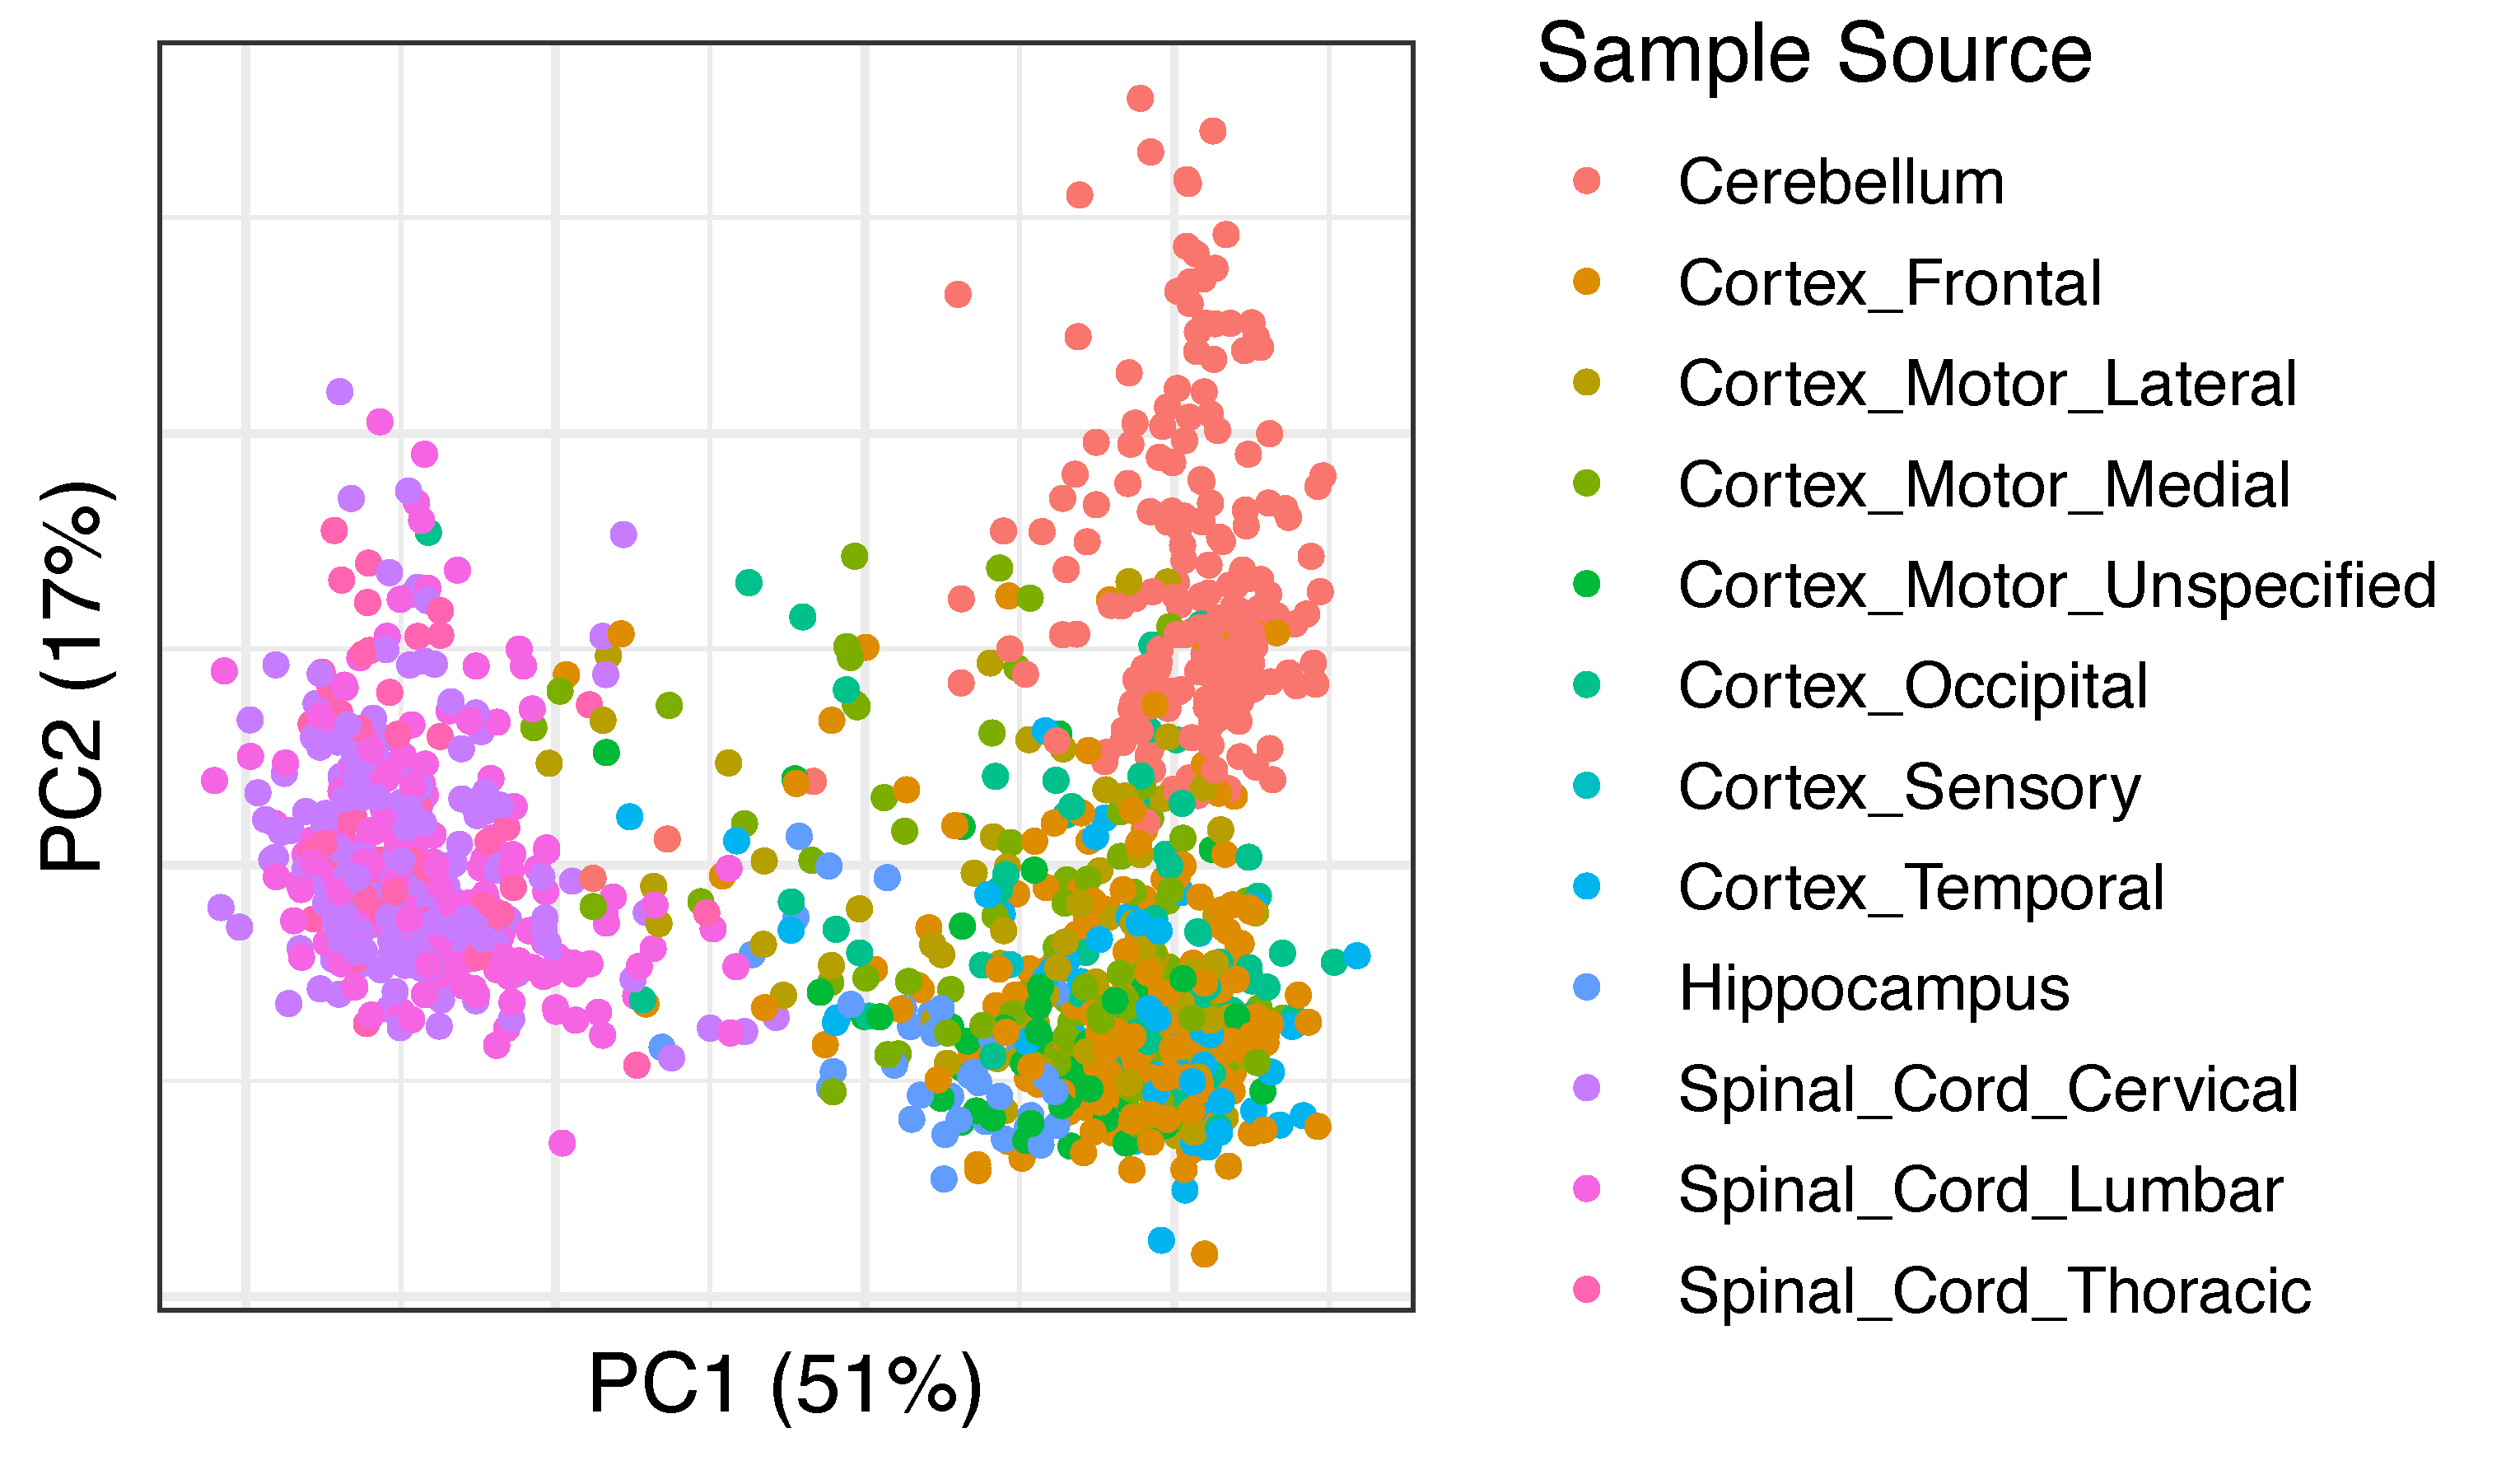
\includegraphics[width=0.75\linewidth]{slides/als_pca.pdf}
  \caption{First two principal components of gene expression in post-mortem central nervous system samples from an ALS cohort, coloured by tissue of origin. Percentages give the proportion of variance explained by each component. Samples group by tissue: spinal cord (left), cerebellum (top right) and other brain regions (bottom right). From the author's analysis.}
  \label{fig:als_pca}
\end{figure}

\subsection{Single-cell RNA-seq}

Bulk RNA-seq (Chapter 1) measures the average expression over all the cells in a sample. Single-cell RNA-seq (scRNA-seq) measures expression in each cell separately, and clustering cells into cell types is one of its central tasks. The most widely used technologies isolate cells in droplets~\citep{macosko2015,klein2015,zheng2017} (Figure~\ref{fig:scrnaseq}). A tissue is dissociated into a suspension of single cells, which flows through a microfluidic device that encapsulates cells into aqueous droplets in oil, each with a gel bead. Every bead carries many copies of a DNA oligonucleotide consisting of a \emph{cell barcode}, shared by all oligonucleotides on that bead, a \emph{unique molecular identifier} (UMI), different for every oligonucleotide, and a poly(T) tail that captures the poly(A) tail of messenger RNA. Inside the droplet the cell is lysed, its mRNA molecules hybridize to the oligonucleotides, and reverse transcription produces cDNA tagged with the cell barcode and a UMI. The droplets are then broken and the cDNA from all cells is pooled, amplified by PCR and sequenced. After sequencing, the cell barcode tells us which cell each read came from, and the UMI lets us collapse PCR duplicates: reads with the same barcode, UMI and gene came from the same original molecule. The result is a matrix of UMI counts, cells by genes.

\begin{figure}[!htbp]
  \centering
  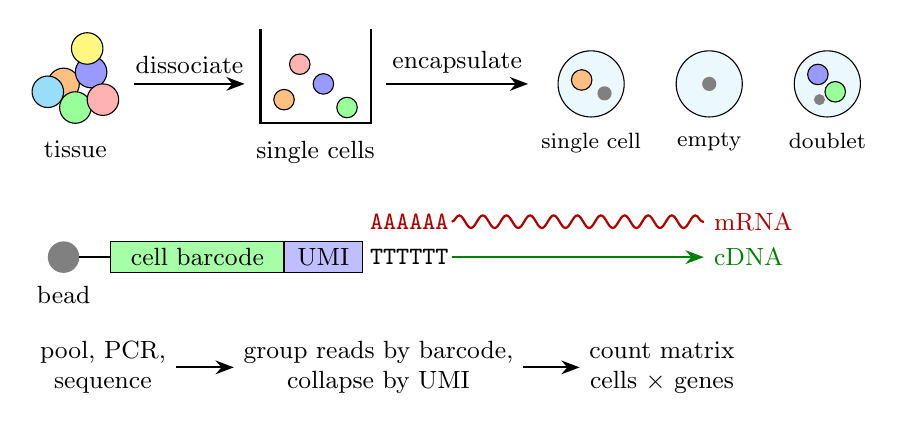
\begin{tikzpicture}[>=Stealth, every node/.style={font=\small}]
    % tissue -> suspension -> droplets
    \foreach \x/\y/\c in {0/0/orange!50, 0.35/0.15/blue!40, 0.15/-0.3/green!40, 0.5/-0.2/red!30, -0.2/-0.1/cyan!40, 0.3/0.45/yellow!50}
      \draw[fill=\c] (\x,\y) circle (0.2);
    \node[below] at (0.15,-0.6) {tissue};
    \draw[->, thick] (0.9,0) -- node[above] {dissociate} (2.3,0);
    \draw[thick] (2.5,0.7) -- (2.5,-0.5) -- (3.9,-0.5) -- (3.9,0.7);
    \foreach \x/\y/\c in {2.8/-0.2/orange!50, 3.3/0.0/blue!40, 3.6/-0.3/green!40, 3.0/0.25/red!30}
      \draw[fill=\c] (\x,\y) circle (0.13);
    \node[below] at (3.2,-0.6) {single cells};
    \draw[->, thick] (4.1,0) -- node[above] {encapsulate} (5.9,0);
    % droplets
    \begin{scope}[xshift=6.7cm, every node/.style={font=\footnotesize}]
      \draw[fill=cyan!8] (0,0) circle (0.42); \draw[fill=orange!50] (-0.12,0.05) circle (0.13); \fill[gray] (0.17,-0.12) circle (0.09);
      \node[below] at (0,-0.5) {single cell};
      \draw[fill=cyan!8] (1.5,0) circle (0.42); \fill[gray] (1.5,0) circle (0.09);
      \node[below] at (1.5,-0.5) {empty};
      \draw[fill=cyan!8] (3.0,0) circle (0.42); \draw[fill=blue!40] (2.88,0.12) circle (0.13); \draw[fill=green!40] (3.1,-0.1) circle (0.13);
      \fill[gray] (2.9,-0.2) circle (0.07);
      \node[below] at (3.0,-0.5) {doublet};
    \end{scope}
    % oligo
    \begin{scope}[yshift=-2.2cm]
      \fill[gray] (0,0) circle (0.2); \node[below] at (0,-0.25) {bead};
      \draw[thick] (0.2,0) -- (0.6,0);
      \draw[fill=green!35] (0.6,-0.2) rectangle (2.8,0.2); \node at (1.7,0) {cell barcode};
      \draw[fill=blue!25] (2.8,-0.2) rectangle (3.8,0.2); \node at (3.3,0) {UMI};
      \node[right, inner sep=1pt] (tt) at (3.85,0) {\texttt{TTTTTT}};
      \node[right, inner sep=1pt, red!70!black] (aa) at (3.85,0.45) {\texttt{AAAAAA}};
      \draw[red!70!black, thick, decorate, decoration={snake, amplitude=0.8mm, segment length=3mm}] (aa.east) -- ++(3.2,0)
        node[right] {mRNA};
      \draw[green!50!black, thick, ->] (tt.east) -- ++(3.2,0) node[right] {cDNA};
    \end{scope}
    % downstream
    \begin{scope}[yshift=-3.6cm]
      \node[align=center] (pool) at (0.5,0) {pool, PCR,\\sequence};
      \node[align=center] (dem) at (4.0,0) {group reads by barcode,\\collapse by UMI};
      \node[align=center] (mat) at (7.6,0) {count matrix\\cells $\times$ genes};
      \draw[->, thick] (pool) -- (dem); \draw[->, thick] (dem) -- (mat);
    \end{scope}
  \end{tikzpicture}
  \caption{Droplet-based single-cell RNA-seq. Cells are encapsulated in droplets with barcoded beads (top). Some droplets contain no cell and some contain two (doublets). Each bead oligonucleotide carries a cell barcode, a unique molecular identifier (UMI) and a poly(T) sequence that captures mRNA, which is reverse transcribed into tagged cDNA (middle). After sequencing, reads are assigned to cells by barcode and duplicates are collapsed by UMI (bottom).}
  \label{fig:scrnaseq}
\end{figure}

Encapsulation is random, so some droplets contain no cell, and their barcodes capture only ambient RNA that leaked from other cells, while others contain two or more cells, called \emph{doublets}. Both must be filtered out. Droplets are not the only option. Earlier methods used plates or microfluidic chambers, with lower throughput. \emph{Combinatorial indexing} methods such as sci-RNA-seq~\citep{cao2017} and SPLiT-seq~\citep{rosenberg2018} use the cells themselves as compartments: cells are split across wells, a well-specific barcode is added, the cells are pooled and split again, and after several rounds each cell carries a combination of barcodes that is very likely unique. This scales to more than a million cells per experiment. Related assays measure other modalities in single cells, such as chromatin accessibility (scATAC-seq), and some measure several modalities in the same cell, for example RNA and chromatin accessibility, or RNA and surface proteins~\citep{stoeckius2017}.

A typical scRNA-seq analysis has the following steps:
\begin{enumerate}
  \item quality control: removing empty droplets, doublets and low-quality cells, and selecting genes;
  \item optionally, integrating several data sets and correcting batch effects;
  \item dimensionality reduction (usually PCA) and visualization (usually UMAP or t-SNE);
  \item clustering cells, and annotating the clusters as cell types using marker genes;
  \item downstream analyses, such as differential expression between cell types, ``pseudobulk'' analyses that sum counts over the cells of each type in each sample, and gene regulatory network inference.
\end{enumerate}
The main computational challenges are scale, with millions of cells, and noise: each cell yields only a few thousand UMIs spread over tens of thousands of genes, so most entries of the count matrix are zero.

Figure~\ref{fig:pbmc} shows the result of such a pipeline on 2700 peripheral blood mononuclear cells (PBMCs), from a widely used tutorial for the Seurat package~\citep{seurat_pbmc,hao2021}. The clusters correspond to immune cell types, such as T cells, B cells, natural killer cells and monocytes. The clustering is computed with a graph-based method (Section~\ref{sec:graph}) in the space of the top principal components, and the two-dimensional UMAP embedding is used only for display. Clustering directly in a UMAP or t-SNE embedding is a mistake. These methods distort distances and densities in order to fit the data into two dimensions, so groups in the embedding can be artefacts and real groups can be merged.

\begin{figure}[!htbp]
  \centering
  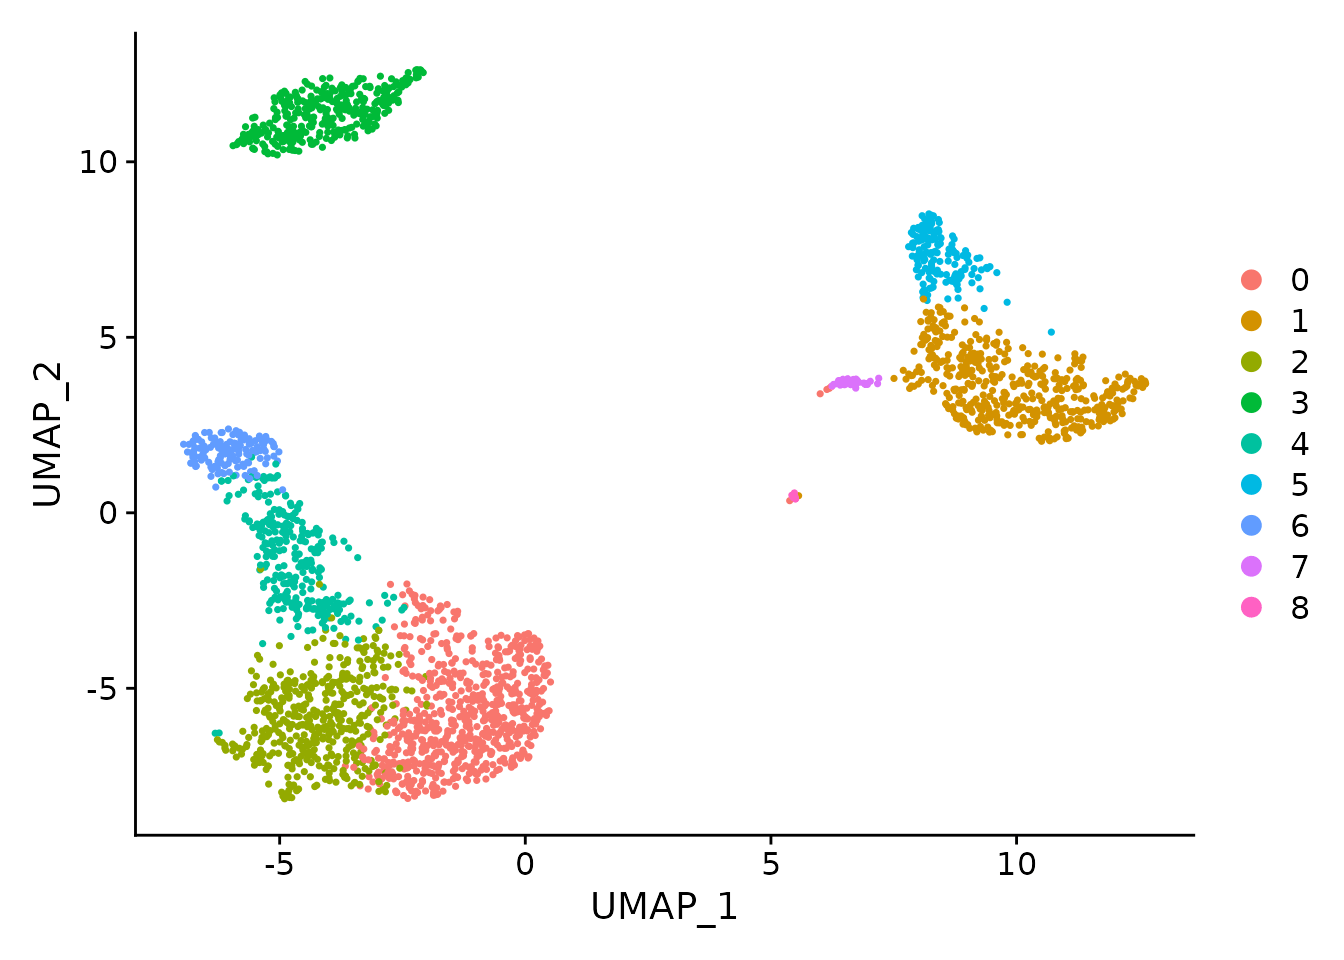
\includegraphics[width=0.6\linewidth]{slides/pbmc3k_umap.png}
  \caption{Clusters of 2700 peripheral blood mononuclear cells shown in a two-dimensional UMAP embedding. The clusters (colours) were found by graph-based clustering in principal component space, not in the UMAP space. Reproduced from the Seurat PBMC 3k tutorial~\citep{seurat_pbmc}.}
  \label{fig:pbmc}
\end{figure}

%======================================================================
\section{The Gaussian mixture model}
\label{sec:gmm}
%======================================================================

Rather than designing a clustering algorithm directly, we start from a generative model: a description of a random process that could have produced the data. Fitting the model to data then gives the algorithm. Let $N$ be the number of data points (cells or samples) and $P$ the number of features (genes), with $\vx_i\in\R^P$ the features of data point $i$ and $\mX\in\R^{N\times P}$ the matrix whose $i$-th row is $\vx_i^\top$. Assume there are $K$ clusters, and that cluster $k\in\{1,\dots,K\}$ has a centre $\vmu_k\in\R^P$. The generative process is, for each data point $i=1,\dots,N$,
\begin{enumerate}
  \item randomly choose a cluster $c_i\in\{1,\dots,K\}$, with $p(c_i=k)=\pi_k$;
  \item sample $\vx_i\sim\Normal(\vmu_{c_i},\sigma^2\mI)$.
\end{enumerate}
The \emph{mixing proportions} $\vpi=(\pi_1,\dots,\pi_K)$ satisfy $\pi_k\geq 0$ and $\sum_k\pi_k=1$; for now we take them equal, $\pi_k=1/K$. The \emph{cluster assignment} $c_i$ is a latent variable: it is part of the model but not observed. Each cluster is a spherical Gaussian with variance $\sigma^2$ in every direction, so data points scatter around their centre in a ball of radius of order $\sigma$ (Figure~\ref{fig:gmm_gen}). We write $\vmu=(\vmu_1,\dots,\vmu_K)$ and $\vc=(c_1,\dots,c_N)$. Figure~\ref{fig:gmm_gen} also shows the model as a graphical model: the latent $c_i$ and observed $\vx_i$ are repeated for each data point, while $\vmu$ and $\sigma^2$ are shared parameters.

\begin{figure}[!htbp]
  \centering
  \begin{minipage}[c]{0.55\linewidth}
    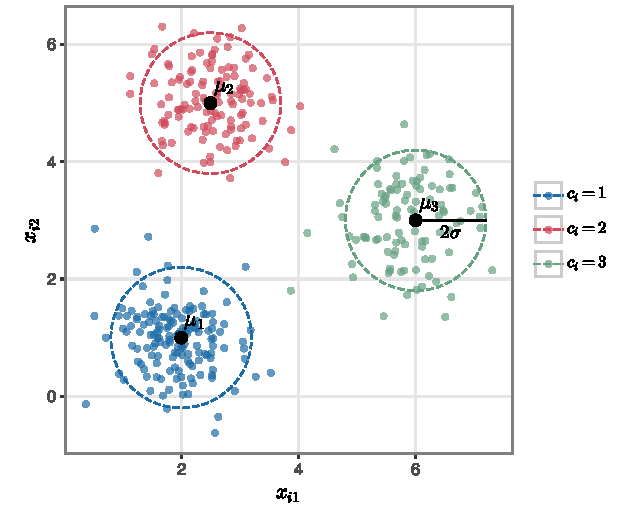
\includegraphics[width=\linewidth]{mixture_generative.pdf}
  \end{minipage}\hfill
  \begin{minipage}[c]{0.4\linewidth}
    \centering
    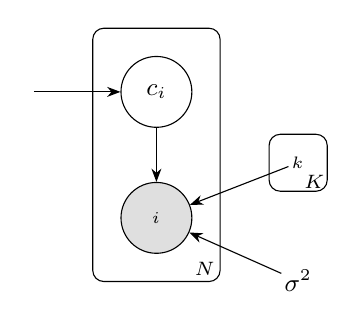
\begin{tikzpicture}[>=Stealth, every node/.style={font=\small},
        latent/.style={circle, draw, minimum size=0.9cm},
        obs/.style={circle, draw, fill=gray!25, minimum size=0.9cm},
        par/.style={inner sep=1pt}]
      \node[latent] (c) at (0,1.6) {$c_i$};
      \node[obs] (x) at (0,0) {$\vx_i$};
      \node[par] (pi) at (-1.6,1.6) {$\vpi$};
      \node[par] (mu) at (1.8,0.7) {$\vmu_k$};
      \node[par] (s) at (1.8,-0.8) {$\sigma^2$};
      \draw[->] (pi) -- (c); \draw[->] (c) -- (x); \draw[->] (mu) -- (x); \draw[->] (s) -- (x);
      \node[draw, rounded corners, fit=(c)(x), inner sep=10pt, label={[anchor=south east, font=\scriptsize, inner sep=2pt]south east:$N$}] {};
      \node[draw, rounded corners, fit=(mu), inner sep=7pt, label={[anchor=south east, font=\scriptsize, inner sep=1pt]south east:$K$}] {};
    \end{tikzpicture}
  \end{minipage}
  \caption{The spherical Gaussian mixture model. Left: simulated data from $K=3$ clusters in $P=2$ dimensions, coloured by the true assignment $c_i$, with the centres $\vmu_k$ and circles of radius $2\sigma$. Right: the model as a graphical model. Shaded nodes are observed, plates denote repetition.}
  \label{fig:gmm_gen}
\end{figure}

\subsection{The likelihood}

If we knew the assignments $\vc$, the likelihood of the centres would be
\begin{equation}
  p(\mX\mid\vmu,\vc) = \prod_{i=1}^N p(\vx_i\mid\vmu,c_i) = \prod_{i=1}^N\Normal(\vx_i\mid\vmu_{c_i},\sigma^2\mI).
\end{equation}
It is convenient to encode the assignments as indicators. Let $r_{ik}=\ind[c_i=k]$, which is 1 if data point $i$ is in cluster $k$ and 0 otherwise, so that each row of the $N\times K$ matrix $(r_{ik})$ has exactly one 1. Raising each factor to the power $r_{ik}$ picks out the right cluster,
\begin{equation}
  p(\mX\mid\vmu,\vc) = \prod_{i=1}^N\prod_{k=1}^K\Normal(\vx_i\mid\vmu_k,\sigma^2\mI)^{r_{ik}},
\end{equation}
and the log likelihood is
\begin{equation}
  \log p(\mX\mid\vmu,\vc) = \sum_{i=1}^N\sum_{k=1}^K r_{ik}\log\Normal(\vx_i\mid\vmu_k,\sigma^2\mI)
  = \sum_{i=1}^N\sum_{k=1}^K r_{ik}\left[-\frac{P}{2}\log 2\pi\sigma^2 - \frac{1}{2\sigma^2}\|\vx_i-\vmu_k\|^2\right].
  \label{eq:complete_loglik}
\end{equation}
Since $\sum_k r_{ik}=1$, the first term sums to $-\frac{NP}{2}\log 2\pi\sigma^2$, which does not depend on $\vmu$ or $\vc$.

%======================================================================
\section{K-means}
\label{sec:kmeans}
%======================================================================

\subsection{The algorithm}

Treat both the centres $\vmu$ and the assignments $\vc$ as unknowns to be estimated by maximum likelihood. Multiplying~\eqref{eq:complete_loglik} by $-2\sigma^2$ and dropping the constant gives the loss
\begin{equation}
  L(\vmu,\vc) = -2\sigma^2\log p(\mX\mid\vmu,\vc) + \text{const} = \sum_{i=1}^N\sum_{k=1}^K r_{ik}\|\vx_i-\vmu_k\|^2 ,
  \label{eq:kmeans_loss}
\end{equation}
the total squared distance from each point to its assigned centre, also called the \emph{within-cluster sum of squares}. Minimizing $L$ jointly over $\vmu$ and $\vc$ is hard, because $\vc$ is discrete and there are $K^N$ possible assignments; in general the problem is NP-hard~\citep{aloise2009}. But each block of variables is easy to optimize with the other held fixed, which suggests alternating between them, a form of coordinate descent.
\begin{enumerate}
  \item \emph{Assignment step.} With $\vmu$ fixed, $L$ is a sum of separate terms for each data point, and the term for point $i$ is $\|\vx_i-\vmu_{c_i}\|^2$. It is minimized by assigning each point to its nearest centre,
  \begin{equation}
    c_i = \argmin_k\|\vx_i-\vmu_k\|^2 .
  \end{equation}
  \item \emph{Update step.} With $\vc$ fixed, $L$ is a sum of separate quadratics in each $\vmu_k$. Setting the gradient to zero,
  \begin{equation}
    \nabla_{\vmu_k}L = -2\sum_{i=1}^N r_{ik}(\vx_i-\vmu_k) = 0
    \quad\Rightarrow\quad
    \vmu_k = \frac{\sum_{i}r_{ik}\vx_i}{\sum_i r_{ik}} ,
    \label{eq:kmeans_update}
  \end{equation}
  so each centre moves to the mean of the points assigned to it. The denominator $N_k=\sum_i r_{ik}$ is the number of points in cluster $k$.
\end{enumerate}
Iterating these two steps is the K-means algorithm (Algorithm~\ref{alg:kmeans})~\citep{lloyd1982,macqueen1967}. Each step minimizes $L$ over one block of variables, so $L$ never increases. Because there are finitely many assignments and $L$ strictly decreases whenever the assignments change, the algorithm stops after a finite number of iterations at a point where neither step changes anything. This is a local minimum of $L$, not necessarily the global one. Each iteration costs $O(NKP)$ operations, for the distances between every point and every centre, which makes K-means fast enough for millions of points. The assignment step partitions $\R^P$ into the regions closest to each centre (Voronoi cells), whose boundaries are hyperplanes, so K-means clusters are always separated by linear boundaries.

\begin{algorithm}[!htbp]
  \caption{K-means}
  \label{alg:kmeans}
  \begin{algorithmic}[1]
    \State Initialize centres $\vmu_1,\dots,\vmu_K$, e.g.\ with K-means++
    \Repeat
      \For{$i=1,\dots,N$} $c_i\gets\argmin_k\|\vx_i-\vmu_k\|^2$ \EndFor
      \For{$k=1,\dots,K$} $\vmu_k\gets\frac{1}{N_k}\sum_{i:c_i=k}\vx_i$, \quad $N_k=|\{i:c_i=k\}|$ \EndFor
    \Until{the assignments do not change}
  \end{algorithmic}
\end{algorithm}

Figure~\ref{fig:kmeans_iter} shows K-means on data from three clusters. Starting from poorly placed centres, the first assignment step splits the data badly, but after two updates the centres have moved to the three groups and the algorithm has converged. The last panel shows a run from a different starting point that converges to a poor local minimum: one centre covers two true clusters and two centres split the third. Its loss is five times larger.

\begin{figure}[!htbp]
  \centering
  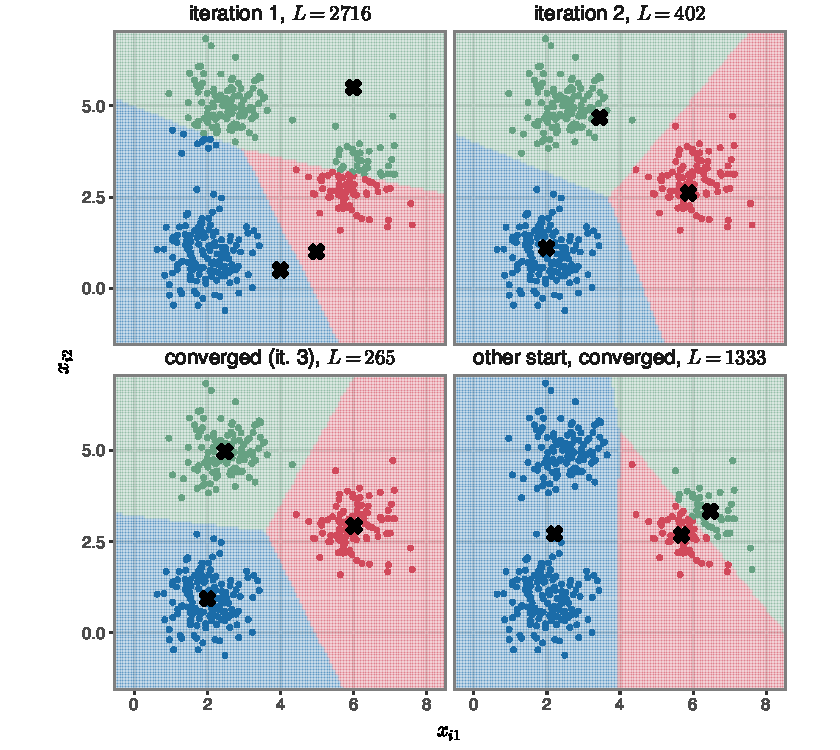
\includegraphics[width=0.8\linewidth]{kmeans_iterations.pdf}
  \caption{K-means on simulated data with three clusters. Each panel shows the current centres (crosses), the regions of the plane closest to each centre (shaded) and the resulting assignments (point colours), with the loss $L$ of~\eqref{eq:kmeans_loss}. The first three panels are successive iterations from one initialization, which converges to the correct clusters. The last panel is the converged result from a different initialization, a poor local minimum.}
  \label{fig:kmeans_iter}
\end{figure}

\subsection{Practical points}

\paragraph{Initialization.} Because K-means finds a local minimum, the starting point matters. A simple choice is to pick $K$ data points at random as initial centres, but this often places two centres in the same true cluster and none in another (Figure~\ref{fig:kmeanspp}, left), and K-means cannot recover from this because centres only move locally. \emph{K-means++}~\citep{arthur2007} spreads the initial centres out. The first centre is a data point chosen uniformly at random. Each subsequent centre is a data point chosen at random with probability proportional to $D(\vx_i)^2$, the squared distance from $\vx_i$ to the nearest centre chosen so far. Points far from the existing centres, which are likely to be in an uncovered cluster, are therefore likely to be chosen. \citet{arthur2007} showed that the expected loss of the K-means++ initialization alone is within a factor $O(\log K)$ of the optimum. It is also good practice to run K-means from several (for example 10) initializations and keep the solution with the lowest loss; standard implementations do this by default.

\begin{figure}[!htbp]
  \centering
  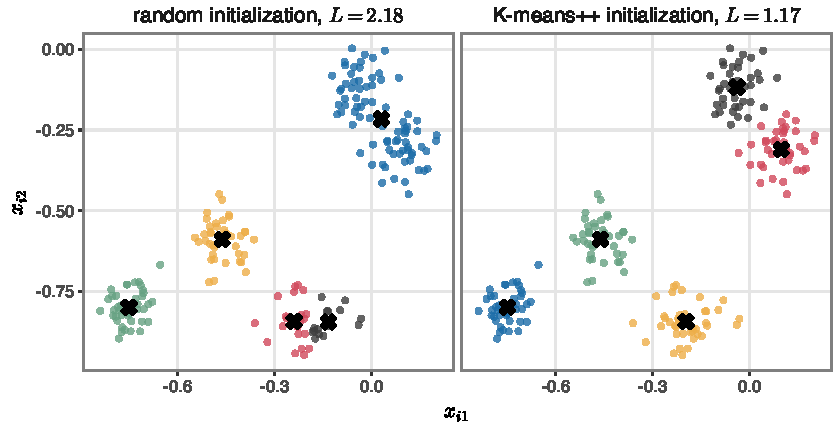
\includegraphics[width=0.85\linewidth]{kmeanspp.pdf}
  \caption{K-means with $K=5$ on $N=200$ simulated points. Left: from a random initialization, K-means converges to a local minimum that merges two clusters (top right) and splits another (bottom). Right: from a K-means++ initialization it finds the five clusters, with lower loss $L$.}
  \label{fig:kmeanspp}
\end{figure}

\paragraph{Choosing $K$.} The number of clusters is a hyperparameter, and it cannot be chosen by minimizing $L$: the optimal loss can only decrease as $K$ grows, reaching zero when every point is its own cluster (Figure~\ref{fig:choose_k}, left). One informal approach looks for an ``elbow'', the value of $K$ after which $L$ decreases slowly. The \emph{gap statistic}~\citep{tibshirani2001} formalizes this by comparing $\log L_K$, the log of the converged loss with $K$ clusters, with its expected value under a reference distribution with no cluster structure, usually the uniform distribution over the bounding box of the data,
\begin{equation}
  \text{Gap}(K) = \E^*\left[\log L^*_K\right] - \log L_K .
\end{equation}
The expectation is estimated by clustering $B$ reference data sets of the same size, and $s_K$ is the standard deviation of $\log L^*_K$ across them multiplied by $\sqrt{1+1/B}$. The estimate is the smallest $K$ such that $\text{Gap}(K)\geq\text{Gap}(K+1)-s_{K+1}$. Figure~\ref{fig:choose_k} (right) shows the gap statistic correctly choosing $K=4$. Other approaches are manual inspection, for example whether clusters correspond to known cell types; model selection criteria such as BIC for mixture models; and Bayesian nonparametric models, which place a Dirichlet process prior on the mixing proportions~\citep{ferguson1973}. The Dirichlet process allows an unbounded number of clusters, of which a finite number are used by any finite data set, and the posterior over the number of clusters is inferred together with the clusters~\citep{rasmussen2000}. Section~\ref{sec:significance} returns to this question from the point of view of hypothesis testing.

\begin{figure}[!htbp]
  \centering
  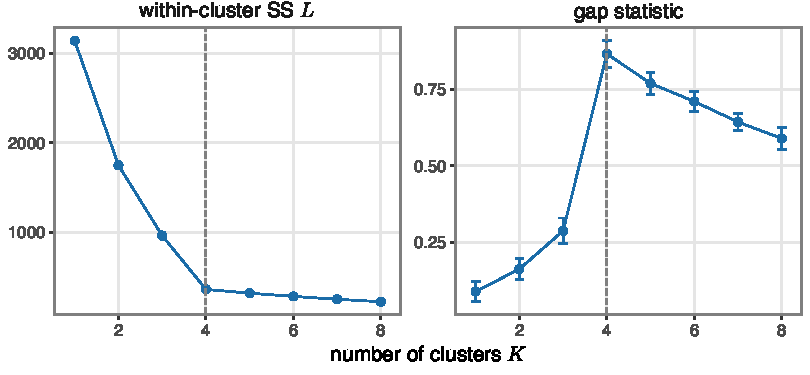
\includegraphics[width=0.85\linewidth]{choose_k.pdf}
  \caption{Choosing the number of clusters for simulated data with four clusters. Left: the K-means loss decreases with $K$, steeply up to $K=4$ and slowly after. Right: the gap statistic with error bars $\pm s_K$ ($B=20$ uniform reference data sets); the rule of \citet{tibshirani2001} selects $K=4$ (dashed line).}
  \label{fig:choose_k}
\end{figure}

\paragraph{Scaling.} K-means uses Euclidean distance, so features on larger scales dominate. For expression data, counts are usually normalized for sequencing depth and log-transformed, and the clustering is run on the top principal components rather than on all genes.

%======================================================================
\section{From hard to soft assignments: expectation-maximization}
\label{sec:em}
%======================================================================

K-means makes a hard decision for every point, even one that lies halfway between two centres. It also treats the assignments $\vc$ as parameters to be optimized, although they are latent variables with a distribution under the model. The principled alternative is to maximize the \emph{marginal likelihood} of the parameters, with the latent variables summed out,
\begin{equation}
  p(\mX\mid\vmu) = \sum_{\vc}p(\mX,\vc\mid\vmu), \qquad
  \log p(\mX\mid\vmu) = \log\sum_{\vc}p(\mX,\vc\mid\vmu),
  \label{eq:marginal}
\end{equation}
where $\sum_{\vc}$ is over all $K^N$ joint assignments. The log of a sum is awkward to maximize directly. The \emph{expectation-maximization} (EM) algorithm~\citep{dempster1977} replaces it with a lower bound that is easy to maximize. We derive it for a general latent variable model with parameters $\theta$, latent variables $\vc$ and data $\mX$, and then specialize to the mixture model, where $\theta=\vmu$.

\subsection{A lower bound from Jensen's inequality}

Let $q(\vc)$ be any probability distribution over the latent variables that is positive wherever $p(\mX,\vc\mid\theta)$ is. Multiplying and dividing by $q(\vc)$ inside the sum,
\begin{equation}
  \log p(\mX\mid\theta) = \log\sum_{\vc}q(\vc)\frac{p(\mX,\vc\mid\theta)}{q(\vc)}
  = \log\E_{q}\left[\frac{p(\mX,\vc\mid\theta)}{q(\vc)}\right].
\end{equation}
Jensen's inequality states that for a concave function $f$ and any random variable $u$, $f(\E[u])\geq\E[f(u)]$: the function of an average is at least the average of the function. Figure~\ref{fig:jensen} shows why for the logarithm. Any chord of a concave curve lies below the curve, and a weighted average of two points on the curve is a point on the chord. Applying Jensen's inequality with $f=\log$,
\begin{equation}
  \log p(\mX\mid\theta) \geq \E_q\left[\log\frac{p(\mX,\vc\mid\theta)}{q(\vc)}\right]
  = \sum_{\vc}q(\vc)\log\frac{p(\mX,\vc\mid\theta)}{q(\vc)} \equiv \mathcal{F}[q,\theta].
  \label{eq:elbo}
\end{equation}
The lower bound $\mathcal{F}$ is a function of both the distribution $q$ and the parameters $\theta$. It is called the \emph{evidence lower bound} (ELBO), or, with the opposite sign, the variational free energy~\citep{neal1998}. EM maximizes $\mathcal{F}$ by alternating between $q$ and $\theta$,
\begin{align}
  \text{E step:}\quad & q \gets \argmax_q\mathcal{F}[q,\theta], \\
  \text{M step:}\quad & \theta \gets \argmax_\theta\mathcal{F}[q,\theta].
\end{align}

\begin{figure}[!htbp]
  \centering
  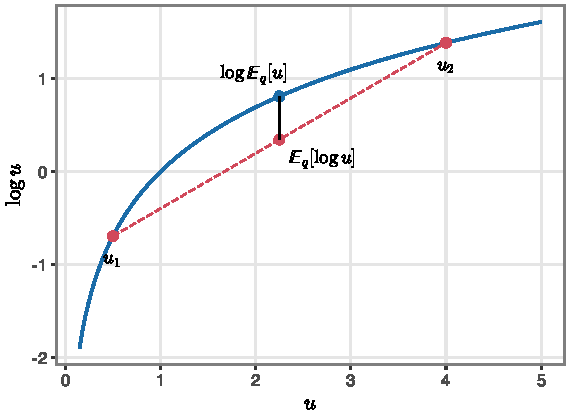
\includegraphics[width=0.5\linewidth]{jensen.pdf}
  \caption{Jensen's inequality for the concave function $\log u$. For a random variable $u$ taking values $u_1$ and $u_2$ with probabilities $q$ and $1-q$ (here $q=0.5$), $\E_q[\log u]$ lies on the chord between $(u_1,\log u_1)$ and $(u_2,\log u_2)$, below $\log\E_q[u]$ on the curve. The vertical segment is the gap in~\eqref{eq:elbo}.}
  \label{fig:jensen}
\end{figure}

\subsection{The E step}

To find the maximizing $q$, write the joint probability as $p(\mX,\vc\mid\theta)=p(\vc\mid\mX,\theta)\,p(\mX\mid\theta)$. Substituting into~\eqref{eq:elbo},
\begin{align}
  \mathcal{F}[q,\theta] &= \sum_{\vc}q(\vc)\log p(\mX\mid\theta) + \sum_{\vc}q(\vc)\log\frac{p(\vc\mid\mX,\theta)}{q(\vc)} \nonumber\\
  &= \log p(\mX\mid\theta) - \KL\left(q(\vc)\,\|\,p(\vc\mid\mX,\theta)\right),
  \label{eq:elbo_kl}
\end{align}
using $\sum_{\vc}q(\vc)=1$, where $\KL(q\|p)=\sum_{\vc}q(\vc)\log\frac{q(\vc)}{p(\vc)}$ is the Kullback-Leibler divergence. The KL divergence is non-negative and is zero only when $q=p$. So the gap between the log marginal likelihood and the bound is exactly $\KL(q\|p(\vc\mid\mX,\theta))$, and the E step sets $q$ to the posterior distribution of the latent variables under the current parameters,
\begin{equation}
  q(\vc) = p(\vc\mid\mX,\theta),
\end{equation}
which makes the bound tight: $\mathcal{F}[q,\theta]=\log p(\mX\mid\theta)$. The name ``expectation step'' comes from computing the expectations under this posterior that the M step needs.

\subsection{The M step}

Expanding the logarithm in~\eqref{eq:elbo},
\begin{equation}
  \mathcal{F}[q,\theta] = \E_q\left[\log p(\mX,\vc\mid\theta)\right] - \E_q\left[\log q(\vc)\right].
\end{equation}
The second term, the entropy of $q$ with a minus sign, does not depend on $\theta$, so the M step is
\begin{equation}
  \theta \gets \argmax_\theta\E_q\left[\log p(\mX,\vc\mid\theta)\right],
\end{equation}
the maximization of the expected complete-data log likelihood. This is usually much easier than maximizing~\eqref{eq:marginal}, because the logarithm acts directly on the joint probability, which for most models is a product of simple terms.

\subsection{EM increases the likelihood}

Let $\theta^{\text{old}}$ be the current parameters, $q$ the posterior computed from them in the E step, and $\theta^{\text{new}}$ the result of the M step. Then
\begin{equation}
  \log p(\mX\mid\theta^{\text{new}}) \geq \mathcal{F}[q,\theta^{\text{new}}] \geq \mathcal{F}[q,\theta^{\text{old}}] = \log p(\mX\mid\theta^{\text{old}}).
\end{equation}
The first inequality is the bound~\eqref{eq:elbo}, the second holds because the M step maximizes $\mathcal{F}$ over $\theta$, and the equality holds because the E step made the bound tight at $\theta^{\text{old}}$. So each EM iteration can only increase the marginal likelihood. Like K-means, EM converges to a local optimum that depends on the initialization, and it is common to initialize EM with the result of K-means.

\subsection{EM for the mixture model}

\paragraph{E step.} By Bayes' rule, the posterior over assignments is
\begin{equation}
  q(\vc) = p(\vc\mid\mX,\vmu) = \frac{p(\mX\mid\vc,\vmu)\,p(\vc)}{p(\mX\mid\vmu)} .
\end{equation}
Both the likelihood $p(\mX\mid\vc,\vmu)=\prod_i p(\vx_i\mid c_i,\vmu)$ and the prior $p(\vc)=\prod_i p(c_i)$, with $p(c_i=k)=1/K$, factorize over data points, so the posterior factorizes too, $q(\vc)=\prod_i q(c_i)$, with
\begin{equation}
  q(c_i=k) = \frac{p(\vx_i\mid c_i=k,\vmu)\,\frac{1}{K}}{\sum_{k'=1}^K p(\vx_i\mid c_i=k',\vmu)\,\frac{1}{K}}
  = \frac{\Normal(\vx_i\mid\vmu_k,\sigma^2\mI)}{\sum_{k'=1}^K\Normal(\vx_i\mid\vmu_{k'},\sigma^2\mI)} .
\end{equation}
We write $r_{ik}=q(c_i=k)$ and call it the \emph{responsibility} of cluster $k$ for point $i$. It replaces the hard indicator of K-means with a probability: $r_{ik}\in[0,1]$ and $\sum_k r_{ik}=1$. Because all clusters share the variance $\sigma^2\mI$, the normalizing constants of the Gaussians cancel and
\begin{equation}
  r_{ik} = \frac{\exp\left(-\|\vx_i-\vmu_k\|^2/2\sigma^2\right)}{\sum_{k'}\exp\left(-\|\vx_i-\vmu_{k'}\|^2/2\sigma^2\right)},
  \label{eq:resp}
\end{equation}
a softmax of the negative squared distances to the centres, scaled by $2\sigma^2$.

\paragraph{M step.} The complete-data log likelihood is~\eqref{eq:complete_loglik} plus the log prior $\sum_i\log p(c_i)$, which does not depend on $\vmu$. Its expectation under $q$ replaces each indicator $\ind[c_i=k]$ by its expectation $r_{ik}$,
\begin{equation}
  \E_q\left[\log p(\mX,\vc\mid\vmu)\right] = -\frac{1}{2\sigma^2}\sum_{i=1}^N\sum_{k=1}^K r_{ik}\|\vx_i-\vmu_k\|^2 + \text{const}.
\end{equation}
This has the same form as the K-means loss~\eqref{eq:kmeans_loss}, so the maximizer has the same form as~\eqref{eq:kmeans_update},
\begin{equation}
  \vmu_k = \frac{\sum_i r_{ik}\vx_i}{\sum_i r_{ik}},
  \label{eq:em_mu}
\end{equation}
now a weighted mean in which every point contributes to every centre in proportion to its responsibility. EM for this model is therefore a ``soft'' or weighted K-means: compute responsibilities~\eqref{eq:resp}, update centres~\eqref{eq:em_mu}, and repeat.

The variance $\sigma^2$ controls how soft the assignments are. As $\sigma^2\to 0$, the softmax in~\eqref{eq:resp} puts all its weight on the nearest centre, $r_{ik}\to\ind[k=\argmin_{k'}\|\vx_i-\vmu_{k'}\|^2]$, and EM reduces to K-means. K-means is thus the zero-variance limit of EM for the spherical Gaussian mixture. Figure~\ref{fig:em_vs_kmeans} compares the two on overlapping clusters. Points far from all centres, or between two of them, receive mixed responsibilities under EM, while K-means forces each into one cluster.

\begin{figure}[!htbp]
  \centering
  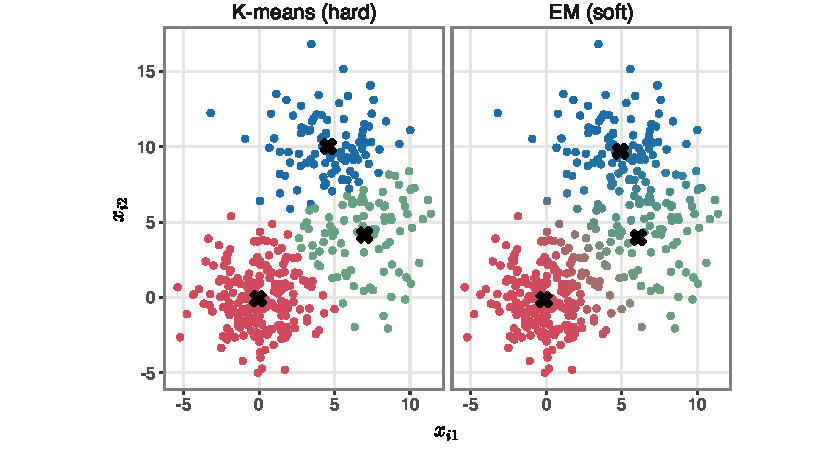
\includegraphics[width=0.85\linewidth]{em_vs_kmeans.pdf}
  \caption{K-means (left) and EM for a spherical Gaussian mixture with fixed $\sigma$ (right) on three overlapping simulated clusters, from the same initialization. On the right each point's colour is a mixture of the three cluster colours weighted by its responsibilities $r_{ik}$, so points between clusters have intermediate colours. Crosses mark the converged centres.}
  \label{fig:em_vs_kmeans}
\end{figure}

\paragraph{Learning the other parameters.} The same M step gives updates for the remaining parameters if we treat them as unknown. With unequal mixing proportions $\pi_k$, the E step becomes $r_{ik}\propto\pi_k\Normal(\vx_i\mid\vmu_k,\sigma^2\mI)$, and the expected complete-data log likelihood gains the term $\sum_i\sum_k r_{ik}\log\pi_k$. Maximizing it subject to $\sum_k\pi_k=1$ with a Lagrange multiplier $\lambda$, $\partial/\partial\pi_k\left[\sum_i r_{ik}\log\pi_k-\lambda\pi_k\right]=0$ gives $\pi_k=\sum_i r_{ik}/\lambda$, and the constraint gives $\lambda=\sum_i\sum_k r_{ik}=N$, so
\begin{equation}
  \pi_k = \frac{1}{N}\sum_{i=1}^N r_{ik},
\end{equation}
the average responsibility of cluster $k$. Differentiating the expectation of~\eqref{eq:complete_loglik} with respect to $\sigma^2$, $-\frac{NP}{2\sigma^2}+\frac{1}{2\sigma^4}\sum_i\sum_k r_{ik}\|\vx_i-\vmu_k\|^2=0$, gives
\begin{equation}
  \sigma^2 = \frac{1}{NP}\sum_{i=1}^N\sum_{k=1}^K r_{ik}\|\vx_i-\vmu_k\|^2 .
\end{equation}
The log marginal likelihood, which EM increases at every iteration and which is useful for monitoring convergence and comparing models, is $\log p(\mX\mid\theta)=\sum_i\log\sum_k\pi_k\Normal(\vx_i\mid\vmu_k,\sigma^2\mI)$. In practice the inner sum is computed with the log-sum-exp trick, $\log\sum_k e^{a_k}=a^*+\log\sum_k e^{a_k-a^*}$ with $a^*=\max_k a_k$, to avoid numerical underflow. Chapter 9 of \citet{bishop2006} gives a complementary treatment of mixture models and EM.

%======================================================================
\section{Why start from a generative model?}
%======================================================================

K-means can be described without any probability, as minimizing the within-cluster sum of squares. Deriving it from a generative model has the advantage that the model makes its assumptions explicit, and so it is easy to change them and rederive the algorithm.
\begin{itemize}
  \item \emph{Cluster shapes.} The spherical model assumes every cluster is a ball of the same size. Each cluster can instead have its own covariance matrix $\mSigma_k\in\R^{P\times P}$, $\vx_i\mid c_i=k\sim\Normal(\vmu_k,\mSigma_k)$. The covariance can be spherical ($\sigma_k^2\mI$), diagonal, full, or low rank plus diagonal, which gives a mixture of factor analysers~\citep{ghahramani1996}, and it can be shared across clusters or separate for each. A full covariance has $P(P+1)/2$ parameters per cluster, which is impossible to estimate for $P=20{,}000$ genes, so the low-rank and diagonal options matter for genomic data.
  \item \emph{Data types.} Count data, such as UMI counts, can be modelled with Poisson or negative binomial distributions instead of Gaussians.
  \item \emph{Uncertainty.} A Bayesian treatment, with priors on the parameters, gives a posterior distribution over cluster assignments and parameters, and the Dirichlet process extends this to an unknown number of clusters.
\end{itemize}

For a Gaussian mixture with full covariances, the E step is $r_{ik}\propto\pi_k\Normal(\vx_i\mid\vmu_k,\mSigma_k)$, where now the normalizing constants $|2\pi\mSigma_k|^{-1/2}$ do not cancel, and the M step updates $\pi_k$ and $\vmu_k$ as before and each covariance to the responsibility-weighted sample covariance,
\begin{equation}
  \mSigma_k = \frac{\sum_i r_{ik}(\vx_i-\vmu_k)(\vx_i-\vmu_k)^\top}{\sum_i r_{ik}}.
\end{equation}
Figure~\ref{fig:gmm_full} shows the effect on elongated clusters. K-means, whose clusters are separated by straight lines equidistant from the centres, cuts the elongated clusters in the wrong places, while the full-covariance mixture recovers them. One caution: the likelihood of a mixture with separate covariances is unbounded. If one component's mean sits on a data point and its covariance shrinks toward zero, the density at that point, and hence the likelihood, goes to infinity. Implementations avoid this degenerate solution by adding a small constant to the diagonal of each $\mSigma_k$, which corresponds to a prior on the covariances.

\begin{figure}[!htbp]
  \centering
  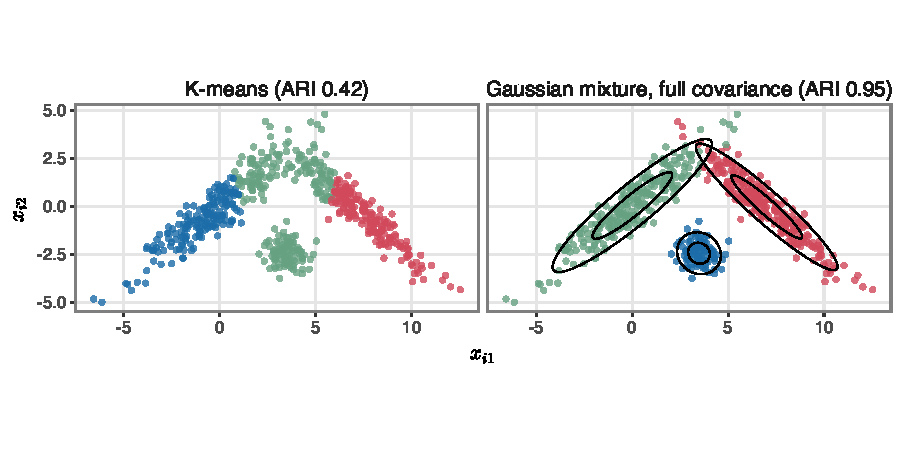
\includegraphics[width=\linewidth]{gmm_full_cov.pdf}
  \caption{Three simulated clusters, two of them elongated. Left: K-means with $K=3$. Right: a Gaussian mixture with a full covariance per cluster fit by EM; ellipses show one and two standard deviations of each fitted component. ARI is the adjusted Rand index between the clustering and the true labels (Section~\ref{sec:significance}), where 1 means perfect agreement.}
  \label{fig:gmm_full}
\end{figure}

%======================================================================
\section{Clustering methods for single-cell data}
\label{sec:scclust}
%======================================================================

K-means and Gaussian mixtures are one family of clustering methods. Figure~\ref{fig:kiselev} compares them with the two other families used for single-cell data, hierarchical clustering and graph-based community detection, on the same data set~\citep{kiselev2019}. The ``true'' labels (panel a) are the cell types reported by the original study. K-means (b) places centres in the densest regions and splits or merges groups of unequal size. Hierarchical clustering (c) builds a tree. Community detection on a $k$-nearest neighbour graph (d, e) gives results that depend on the choice of $k$. No method recovers the reported labels exactly. We describe hierarchical, spectral and graph-based clustering in turn.

\begin{figure}[!htbp]
  \centering
  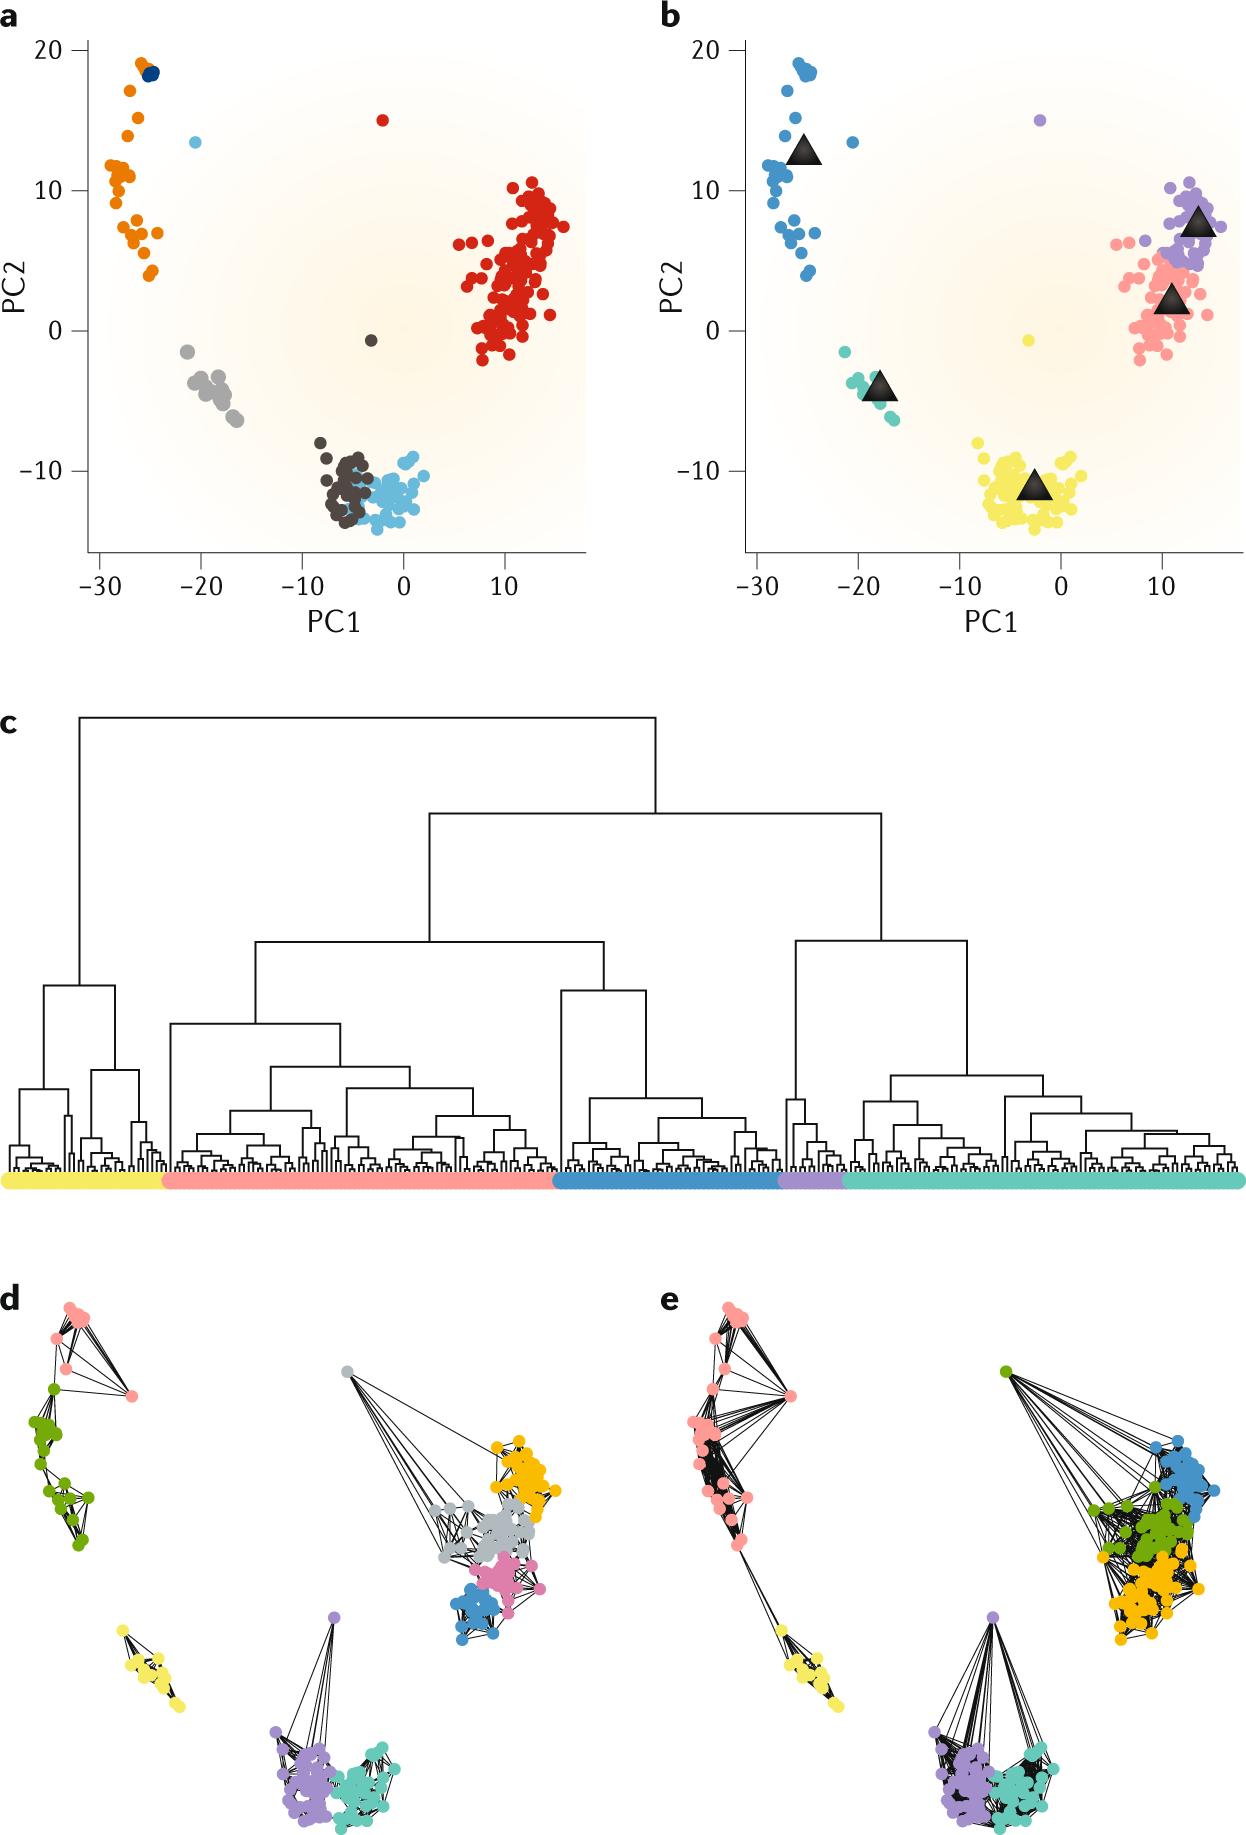
\includegraphics[width=0.75\linewidth]{slides/kiselev2019_fig3.png}
  \caption{Clustering of a single-cell RNA-seq data set shown in principal component space. (a) Cell labels from the original study. (b) K-means; triangles mark the centres. (c) Hierarchical clustering. (d, e) Community detection (Louvain) on $k$-nearest neighbour graphs with $k=5$ and $k=10$. Reproduced from \citet{kiselev2019}.}
  \label{fig:kiselev}
\end{figure}

\subsection{Hierarchical clustering}

Agglomerative hierarchical clustering builds a tree, or \emph{dendrogram}, from the bottom up. It starts with each of the $N$ data points in its own cluster and repeatedly merges the two closest clusters until one cluster remains. The height at which two clusters merge is the distance between them. Cutting the tree at a given height, or at the height that leaves $K$ clusters, gives a flat clustering. The method needs a \emph{linkage}, a rule for the distance between two clusters $A$ and $B$ given distances between points:
\begin{itemize}
  \item \emph{single} linkage, the minimum distance between a point in $A$ and a point in $B$;
  \item \emph{complete} linkage, the maximum such distance;
  \item \emph{average} linkage, the average over all pairs;
  \item \emph{Ward} linkage~\citep{ward1963}, the increase in the within-cluster sum of squares caused by merging,
  \begin{equation}
    w(A,B) = \text{ESS}(A\cup B) - \text{ESS}(A) - \text{ESS}(B), \qquad
    \text{ESS}(A) = \sum_{i\in A}\Big\|\vx_i-\frac{1}{|A|}\sum_{j\in A}\vx_j\Big\|^2 ,
    \label{eq:ward}
  \end{equation}
  where ESS is the error sum of squares and $|A|$ is the number of points in $A$. It can be shown that $w(A,B)=\frac{|A||B|}{|A|+|B|}\|\bar\vx_A-\bar\vx_B\|^2$, where $\bar\vx_A$ is the mean of cluster $A$ (Exercise~\ref{ex:ward}). Ward linkage greedily minimizes the same within-cluster sum of squares as K-means.
\end{itemize}

Hierarchical clustering has two advantages over K-means: it is not iterative and has no randomness, so it gives the same answer every time, and a single tree gives clusterings at every resolution. Its disadvantages are that merges are greedy and can never be undone, that it needs all $N^2$ pairwise distances, which limits it to tens of thousands of points, and that some linkages give very unbalanced clusters. Single linkage is the extreme case. Because two clusters are close if any pair of their points is close, it merges clusters through chains of intermediate points, and outlying points join the tree last, so cutting the tree into $K$ clusters often gives one large cluster and several singletons (Figure~\ref{fig:hclust}). Hierarchical clustering is also widely used to order the rows and columns of heatmaps, as in the breast cancer subtype heatmap of Chapter 1.

\begin{figure}[!htbp]
  \centering
  \begin{subfigure}[b]{\linewidth}
    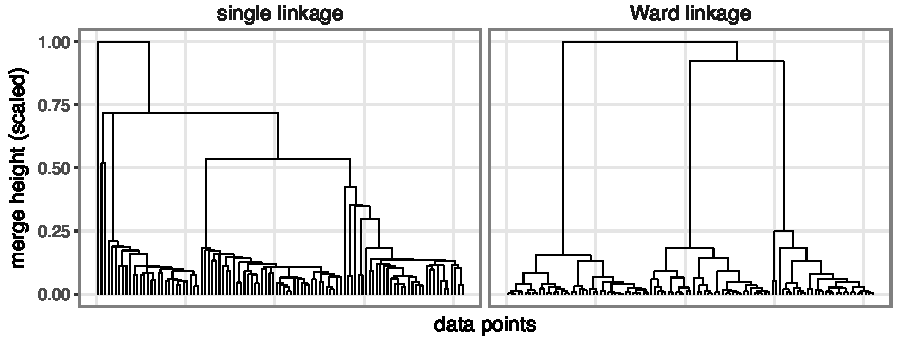
\includegraphics[width=\linewidth]{hclust_dendro.pdf}
    \caption{}
  \end{subfigure}
  \begin{subfigure}[b]{\linewidth}
    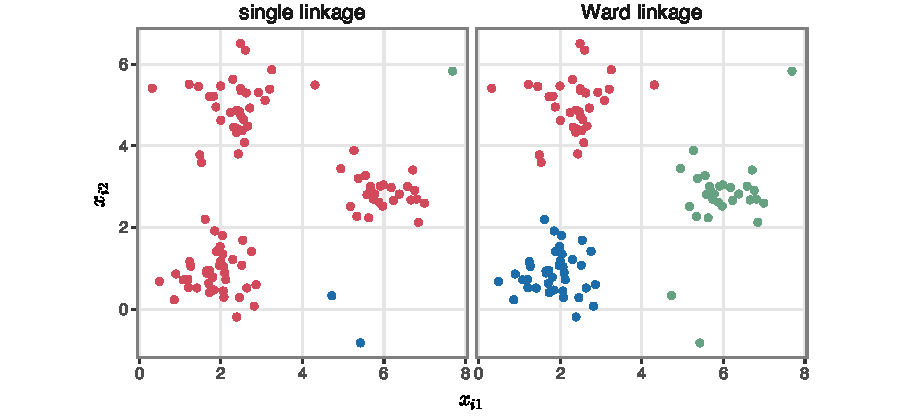
\includegraphics[width=\linewidth]{hclust_scatter.pdf}
    \caption{}
  \end{subfigure}
  \caption{Hierarchical clustering of 103 simulated points (three clusters plus eight scattered points) with single and Ward linkage. (a) Dendrograms, with merge heights scaled to a maximum of one. (b) The three clusters obtained by cutting each tree. Single linkage gives one cluster of 100 points and two clusters made of outlying points; Ward linkage recovers the three groups.}
  \label{fig:hclust}
\end{figure}

\subsection{Spectral clustering}

K-means finds clusters that are compact blobs around a centre. Some clusters are not like this. In the ``two moons'' data of Figure~\ref{fig:spectral}, each cluster is a curved band, and K-means with $K=2$ cuts across both bands with a straight line. What defines each moon is that it is connected: one can walk from any point in it to any other in small steps without leaving the data. \emph{Spectral clustering} formalizes this with a graph~\citep{shi2000,ng2002,vonluxburg2007}, and it uses K-means as its final step.
\begin{enumerate}
  \item Build an $N\times N$ \emph{affinity} matrix $\mA$, with entries
  \begin{equation}
    A_{ij} = \exp\left(-\frac{\|\vx_i-\vx_j\|^2}{2s^2}\right), \quad i\neq j, \qquad A_{ii}=0,
  \end{equation}
  where the bandwidth $s$ sets the distance at which points count as neighbours. Nearby points have $A_{ij}\approx 1$ and distant points $A_{ij}\approx 0$. $\mA$ is the weighted adjacency matrix of a graph whose nodes are the data points.
  \item Compute the \emph{degree} of each node, $D_{ii}=\sum_j A_{ij}$, and form the diagonal matrix $\mD$ and the \emph{graph Laplacian} $\mL=\mD-\mA$.
  \item Eigendecompose $\mL=\mU\mLambda\mU^\top$, where $\mU\in\R^{N\times N}$ is orthogonal and $\mLambda$ is diagonal with the eigenvalues in increasing order, $0=\lambda_1\leq\lambda_2\leq\dots\leq\lambda_N$.
  \item Run K-means on the rows of $\mU_{:,1:K}\in\R^{N\times K}$, the eigenvectors with the $K$ smallest eigenvalues, treating row $i$ as a $K$-dimensional representation of point $i$.
\end{enumerate}

Why does this work? For any vector $\vf\in\R^N$, which assigns a value $f_i$ to each node,
\begin{equation}
  \vf^\top\mL\vf = \sum_i D_{ii}f_i^2 - \sum_{i,j}A_{ij}f_if_j
  = \frac{1}{2}\sum_{i,j}A_{ij}\left(f_i^2+f_j^2-2f_if_j\right)
  = \frac{1}{2}\sum_{i,j}A_{ij}(f_i-f_j)^2 ,
  \label{eq:laplacian_quad}
\end{equation}
where the middle step writes $\sum_i D_{ii}f_i^2=\sum_{i,j}A_{ij}f_i^2$ and symmetrizes using $A_{ij}=A_{ji}$. The quadratic form is small when $\vf$ varies little between strongly connected nodes. It is non-negative, so $\mL$ is positive semi-definite, and it is zero for the constant vector, so $\lambda_1=0$. Now suppose the graph consists of $K$ connected components, with no edges between them. Then~\eqref{eq:laplacian_quad} is zero for any $\vf$ that is constant on each component, so the indicator vectors of the $K$ components are all eigenvectors with eigenvalue 0, and they span the eigenspace of eigenvalue 0. The first $K$ eigenvectors are therefore (an orthogonal rotation of) these indicators, and the rows of $\mU_{:,1:K}$ take only $K$ distinct values, one per component. K-means on the rows recovers the components exactly. Real data are not exactly disconnected, but if the affinity between clusters is weak, the eigenvectors are close to the indicators and K-means on them still separates the clusters. Figure~\ref{fig:spectral} shows this for the two moons. The second eigenvalue is about $4\times 10^{-4}$ and the third about $0.09$, a large gap after $K=2$, and the second eigenvector is nearly constant within each moon.

\begin{figure}[!htbp]
  \centering
  \begin{subfigure}[b]{0.66\linewidth}
    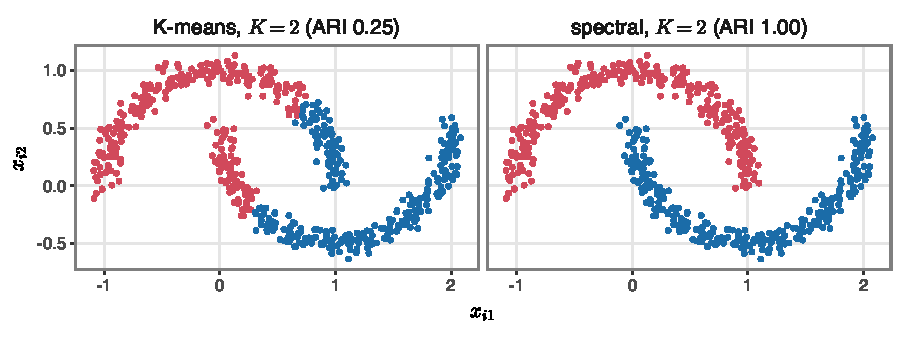
\includegraphics[width=\linewidth]{spectral_moons.pdf}
    \caption{}
  \end{subfigure}\hfill
  \begin{subfigure}[b]{0.33\linewidth}
    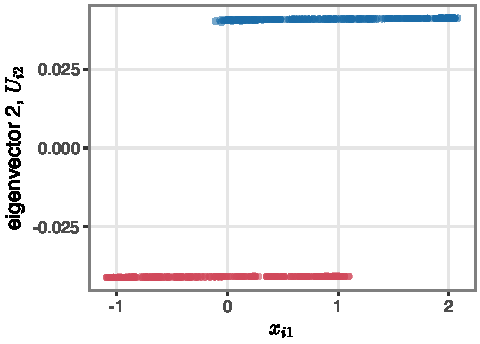
\includegraphics[width=\linewidth]{spectral_embedding.pdf}
    \caption{}
  \end{subfigure}
  \caption{Spectral clustering of the ``two moons'' data ($N=600$). (a) K-means with $K=2$ separates the data with a straight line; spectral clustering with a Gaussian affinity ($s=0.1$) and the unnormalized Laplacian recovers the moons. ARI, adjusted Rand index with the true moons. (b) The second eigenvector of the Laplacian plotted against the first coordinate of each point: it takes one value on each moon, so K-means on the eigenvectors separates them. The first eigenvector is constant.}
  \label{fig:spectral}
\end{figure}

Spectral clustering can also be derived as a continuous relaxation of the problem of cutting the graph into $K$ pieces with small total affinity between pieces and balanced sizes~\citep{vonluxburg2007}. Common variants use a normalized Laplacian, $\mI-\mD^{-1}\mA$~\citep{shi2000} or $\mI-\mD^{-1/2}\mA\mD^{-1/2}$~\citep{ng2002}, which handle clusters of different densities better, and a sparse $k$-nearest neighbour graph instead of the dense Gaussian affinity. A dense eigendecomposition costs $O(N^3)$, so for large $N$ the sparse graph and iterative eigensolvers that compute only the first $K$ eigenvectors are essential. The eigendecomposition is deterministic; randomness enters only through the final K-means step.

\subsection{Graph-based clustering}
\label{sec:graph}

The most widely used clustering methods for single-cell data, the defaults in the Seurat~\citep{hao2021} and Scanpy~\citep{wolf2018} packages, also start from a graph and then look for \emph{communities}, groups of nodes with many edges among themselves and few to the rest of the graph~\citep{levine2015}. The usual pipeline is as follows.
\begin{enumerate}
  \item Reduce the data to the top principal components (typically 10--50).
  \item Build a $k$-nearest neighbour (kNN) graph: connect each cell to the $k$ cells closest to it in PC space. Seurat reweights the edges by the overlap between the two cells' neighbourhoods, which gives a shared nearest neighbour graph.
  \item Partition the graph by maximizing its \emph{modularity} with the Louvain~\citep{blondel2008} or Leiden~\citep{traag2019} algorithm.
\end{enumerate}
For a graph with symmetric weighted adjacency matrix $\mA$, the modularity of an assignment of nodes to communities $c_1,\dots,c_N$ is~\citep{newman2004}
\begin{equation}
  Q = \frac{1}{2m}\sum_{i=1}^N\sum_{j=1}^N\left[A_{ij}-\frac{k_ik_j}{2m}\right]\delta(c_i,c_j),
  \label{eq:modularity}
\end{equation}
where $k_i=\sum_j A_{ij}$ is the degree of node $i$, $2m=\sum_{i,j}A_{ij}$ is twice the total edge weight ($m$ is the number of edges in an unweighted graph), and $\delta(c_i,c_j)$ is 1 if $i$ and $j$ are in the same community and 0 otherwise. The term $k_ik_j/2m$ is the expected weight of the edge between $i$ and $j$ in a random graph with the same degrees. Modularity therefore rewards communities with more internal connections than expected by chance. The Louvain algorithm maximizes $Q$ greedily. It first moves individual nodes to the neighbouring community that most increases $Q$, until no move helps; it then merges each community into a single node and repeats on the smaller graph. The Leiden algorithm refines this and guarantees that communities are connected.

Graph-based clustering does not take the number of clusters as input. The granularity is controlled instead by the number of neighbours $k$ and by a \emph{resolution} parameter $\gamma$, which multiplies the expected term $k_ik_j/2m$ in~\eqref{eq:modularity}: larger $\gamma$ penalizes large communities more and gives more, smaller clusters. Figure~\ref{fig:methods} compares K-means, spectral clustering and Louvain on toy data sets with different geometry. K-means handles the compact clusters but fails on the rings, the moons and the elongated clusters. Spectral clustering recovers the rings and moons. Louvain with default resolution splits every data set, including one with no structure at all, into several pieces that follow the connectivity of the graph. These pieces are often biologically meaningful in single-cell data, where cell types have sub-states, but they show that graph-based methods will find clusters whether or not distinct groups exist. The next section takes up that problem.

\begin{figure}[!htbp]
  \centering
  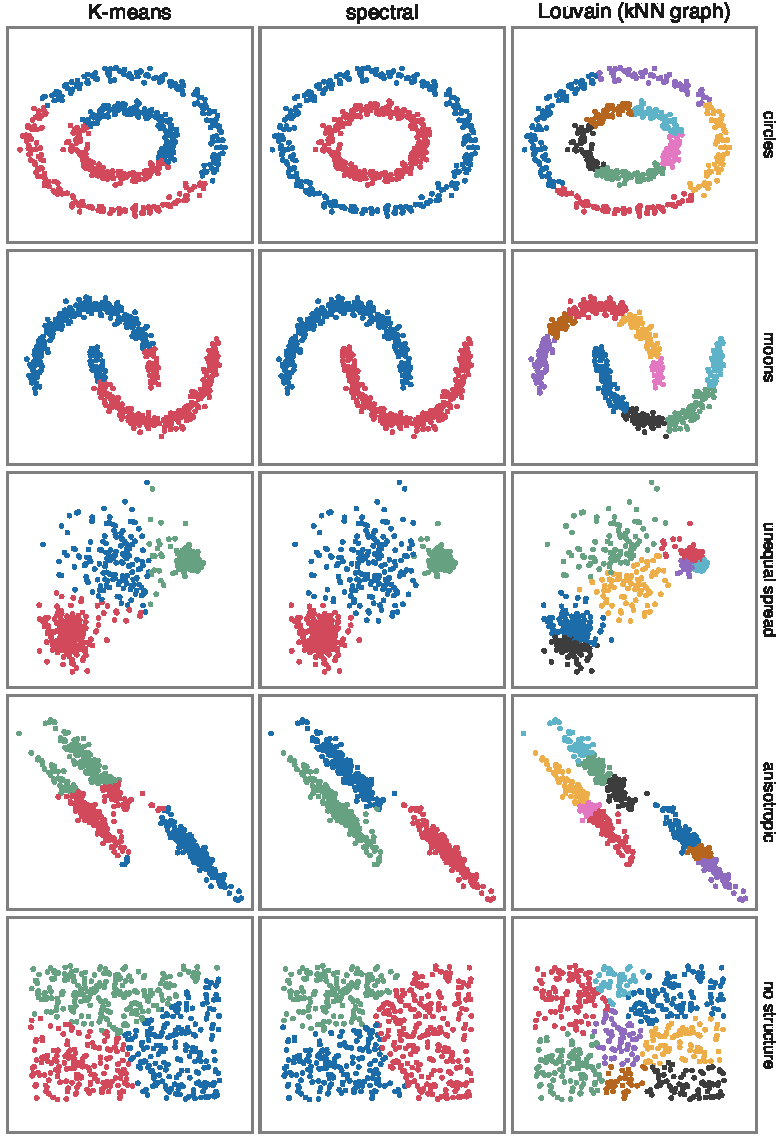
\includegraphics[width=0.72\linewidth]{method_comparison.pdf}
  \caption{K-means, spectral clustering and Louvain community detection on five simulated data sets (rows; $N=600$ each, features standardized). K-means and spectral clustering were given the true number of clusters (2 for circles and moons, 3 otherwise). Spectral clustering uses a symmetric 10-nearest neighbour graph and the normalized Laplacian $\mI-\mD^{-1/2}\mA\mD^{-1/2}$. Louvain uses a symmetric 30-nearest neighbour graph with resolution $\gamma=1$ and chooses the number of clusters itself, finding 7 to 9 clusters in every data set.}
  \label{fig:methods}
\end{figure}

%======================================================================
\section{Are the clusters real?}
\label{sec:significance}
%======================================================================

Every clustering algorithm returns clusters, whether or not the data contain distinct groups. This is a practical problem in single-cell analysis, where clusters are interpreted as cell types or states and then used in downstream analyses. \citet{grabski2023} illustrated it by simulating scRNA-seq counts from a single homogeneous population of cells and running a standard Seurat pipeline with default parameters. Louvain clustering split the cells into nine clusters. Figure~\ref{fig:overcluster} reproduces the effect with a simple simulation: a single population in $P=10$ dimensions, with a long tail along one axis, is divided by Louvain into eight clusters, which in a UMAP or PCA plot look like a plausible gradient of cell states.

\begin{figure}[!htbp]
  \centering
  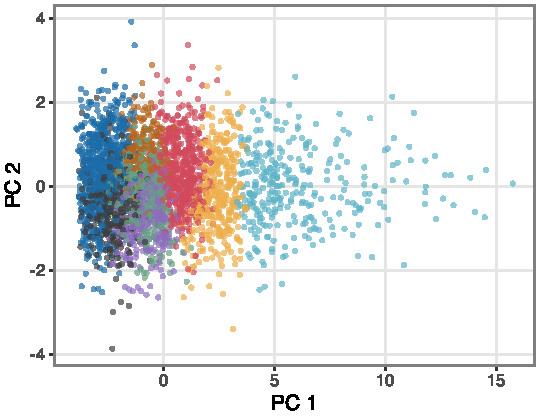
\includegraphics[width=0.5\linewidth]{overclustering.pdf}
  \caption{Louvain clustering (30-nearest neighbour graph, resolution 1) of $N=3000$ points simulated from a single population in $P=10$ dimensions, shown on the first two principal components. Although there is only one population, Louvain reports eight clusters.}
  \label{fig:overcluster}
\end{figure}

\subsection{Measuring clustering accuracy}

To evaluate a clustering against known labels, as in simulations, we need a measure of agreement between two partitions that does not depend on how the clusters are numbered and that allows different numbers of clusters. The \emph{Rand index} is the proportion of the $\binom{N}{2}$ pairs of points on which the two partitions agree, either placing both points in the same cluster or both in different clusters. Even random partitions agree on many pairs, so the \emph{adjusted Rand index} (ARI)~\citep{hubert1985} rescales it so that its expected value is 0 when the partitions are independent and its maximum is 1 for identical partitions,
\begin{equation}
  \text{ARI} = \frac{\text{RI}-\E[\text{RI}]}{\max(\text{RI})-\E[\text{RI}]},
\end{equation}
where the expectation is over random partitions with the same cluster sizes. It can be negative. If the truth is a single cluster, any clustering into more than one cluster has ARI 0.

\subsection{A test for splitting a cluster}

The approach of \citet{grabski2023}, building on statistical significance testing for hierarchical clustering~\citep{kimes2017}, asks for each split of the data into two clusters whether the split is stronger than would be expected if the data came from a single population. The test statistic is the Ward linkage~\eqref{eq:ward} between the two clusters $C_1$ and $C_2$, $w=\text{ESS}(C_1\cup C_2)-\left(\text{ESS}(C_1)+\text{ESS}(C_2)\right)$, the reduction in within-cluster sum of squares achieved by the split. The procedure is as follows.
\begin{enumerate}
  \item Cluster the data into two groups and compute the observed Ward linkage $w$.
  \item Fit a null model, a model of a single population, to the data. \citet{grabski2023} fit a model for the counts; in our simulation the null model is a single multivariate Gaussian with the sample mean and covariance of the data.
  \item Simulate $B$ data sets of the same size from the null model. Cluster each into two groups with the same algorithm and compute its Ward linkage $w_b$, $b=1,\dots,B$.
  \item Compute the p-value $p=(1+\sum_b\ind[w_b\geq w])/(B+1)$.
\end{enumerate}
The crucial step is that the null data sets are clustered with the same algorithm. The two clusters were chosen to be as different as possible, so a naive test of whether their means differ, such as a $t$-test on each gene, would almost always be significant even for a single population. Using the same data to define clusters and to test them is a form of ``double dipping''~\citep{gao2024}. Re-running the clustering on the null data sets accounts for the selection, because the null distribution of $w$ is then the distribution of the best split of a single population.

Figure~\ref{fig:significance} shows the test on two simulated data sets. When the data contain two populations, the observed Ward linkage is larger than any of the 200 null simulations ($p=0.005$, the smallest possible with $B=200$). When the data come from one population with a skewed distribution, the split looks convincing in the PCA plot, but its Ward linkage is typical of the null ($p=0.40$). In the full method the test is applied recursively down a hierarchical clustering tree, starting from the root, and a split is kept only if it is significant, with the significance threshold adjusted to control the family-wise error rate across splits. The same test can be applied to the clusters produced by other methods, such as Louvain, by testing whether pairs of clusters should be merged. In the simulations of \citet{grabski2023}, standard pipelines found between 2 and 15 clusters in data from a single population, and after significance analysis all of them found one. With five true populations the pipelines found between 5 and 11 clusters, and significance analysis brought the numbers closer to five without lowering the ARI.

\begin{figure}[!htbp]
  \centering
  \begin{subfigure}[b]{\linewidth}
    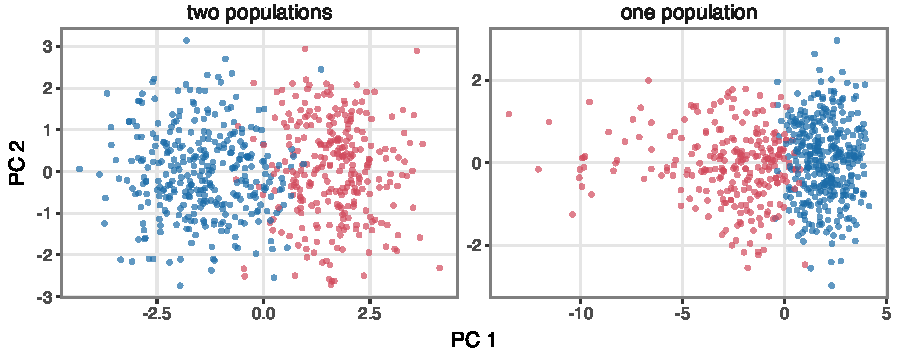
\includegraphics[width=\linewidth]{significance_data.pdf}
    \caption{}
  \end{subfigure}
  \begin{subfigure}[b]{\linewidth}
    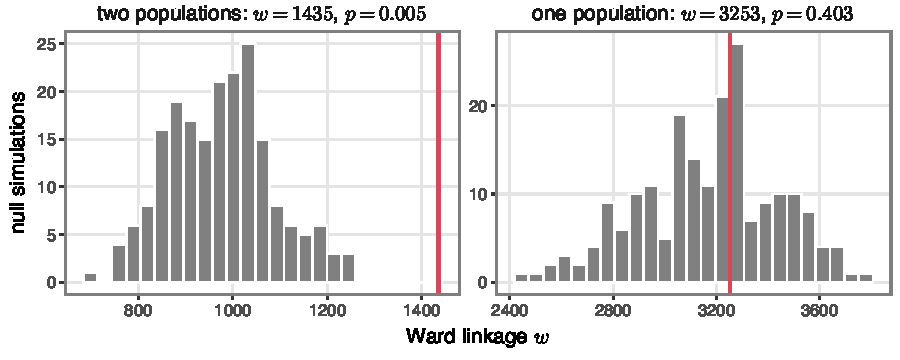
\includegraphics[width=\linewidth]{significance_null.pdf}
    \caption{}
  \end{subfigure}
  \caption{Testing a two-cluster split. (a) Two simulated data sets ($N=600$, $P=10$), each split into two clusters by Ward hierarchical clustering, shown on the first two principal components. Left: two populations whose means differ in one dimension. Right: one population with a skewed first dimension. (b) Ward linkage $w$ of the observed split (red line) compared with its distribution in 200 data sets simulated from a single Gaussian fit to the data and clustered in the same way (histogram). The split is significant for the two-population data and not for the one-population data.}
  \label{fig:significance}
\end{figure}

%======================================================================
\section{Application: molecular subtypes of ALS}
\label{sec:als}
%======================================================================

Amyotrophic lateral sclerosis is a fatal neurodegenerative disease of motor neurons. Patients differ in their age of onset, the site where symptoms start and the rate of progression, which raises the question of whether ALS is one disease or several with distinct molecular mechanisms. \citet{tam2019} addressed this with RNA-seq of 148 post-mortem frontal and motor cortex samples from 77 ALS patients, along with samples from patients with other neurological disorders and from controls. Clustering the ALS samples by gene expression gave three groups (Figure~\ref{fig:tam}), which they named by the genes that distinguish them. ALS-Ox, the largest group, has high expression of genes for oxidative stress and synaptic signalling. ALS-Glia has high expression of microglial, astrocyte and oligodendrocyte markers and inflammatory genes. ALS-TE shows activation of transposable elements (retrotransposons) along with chromatin, spliceosome and proteasome genes.

\begin{figure}[!htbp]
  \centering
  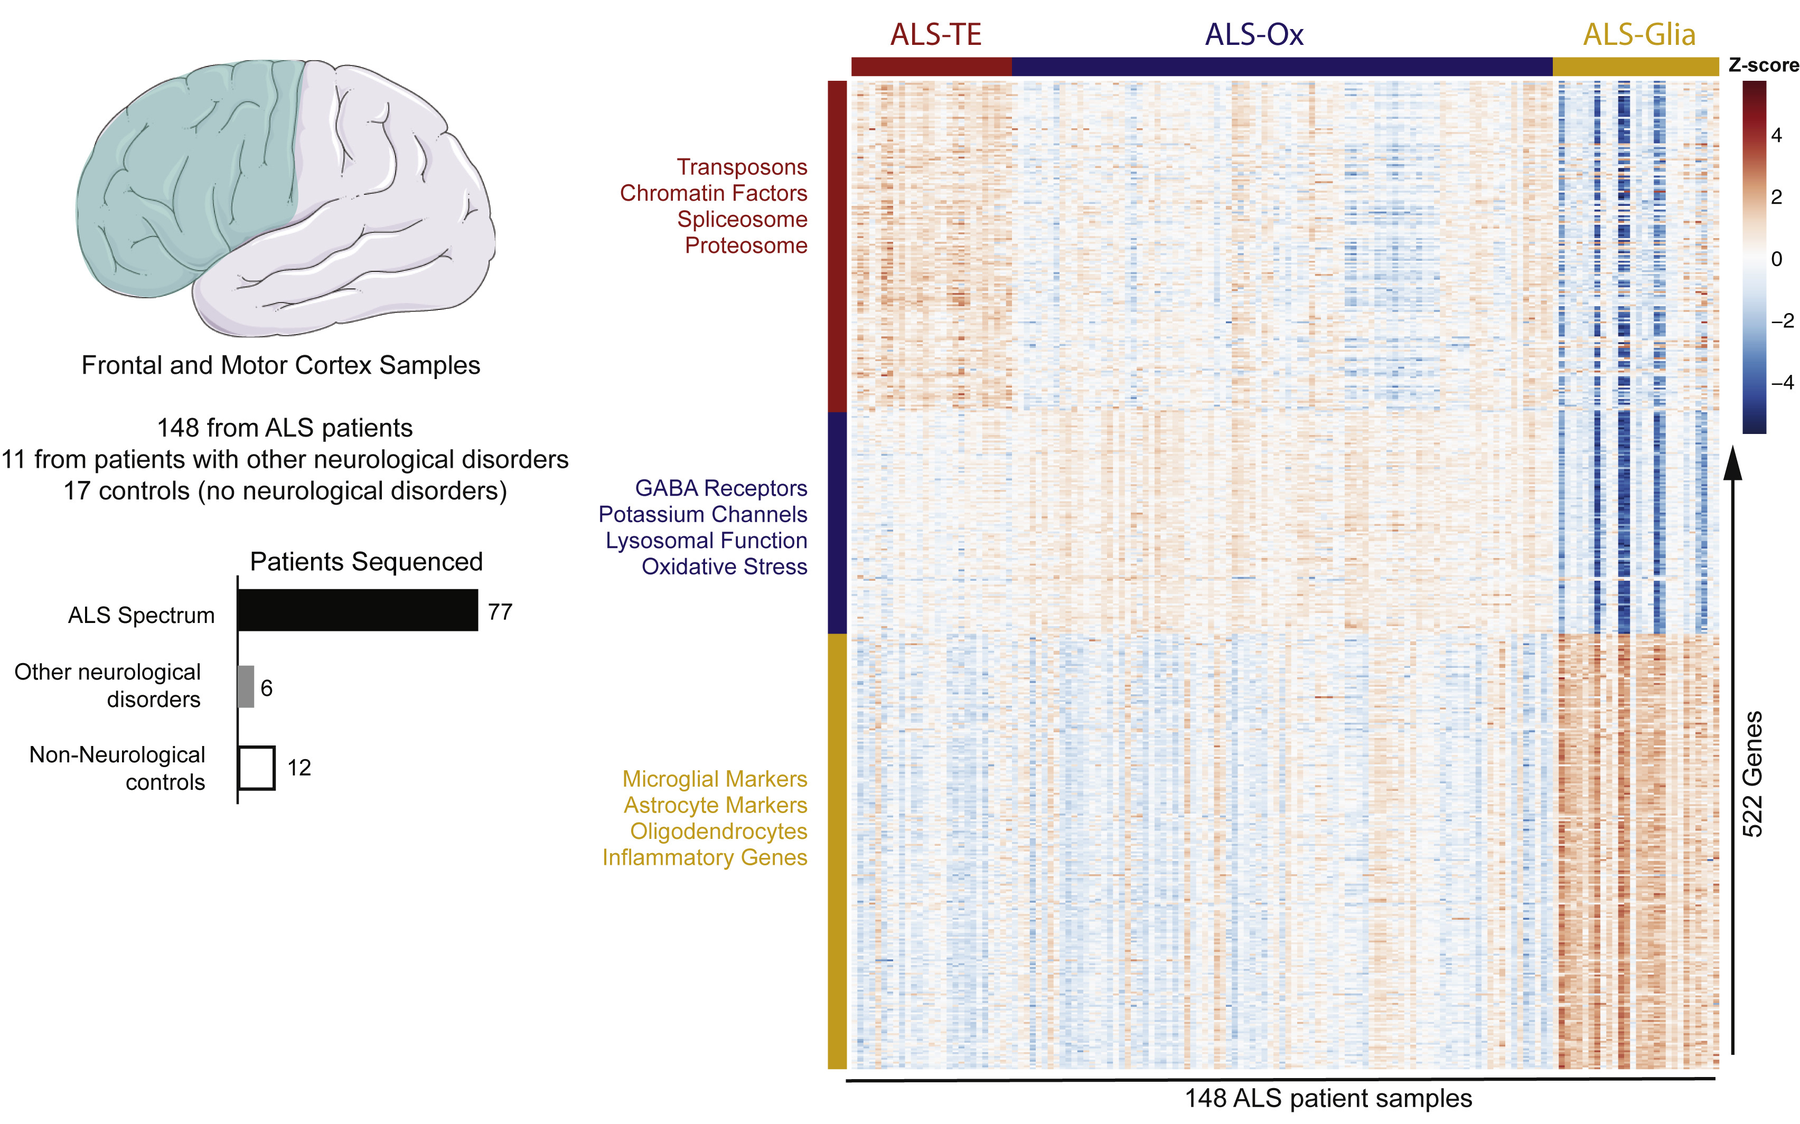
\includegraphics[width=\linewidth]{slides/tam2019_als_subtypes.png}
  \caption{Molecular subtypes of ALS from post-mortem cortex RNA-seq. Left: the cohort. Right: expression ($z$-scores) of 522 genes (rows) that distinguish three clusters of 148 ALS patient samples (columns), labelled ALS-TE, ALS-Ox and ALS-Glia, with the main functional categories of the genes on the left. Reproduced from \citet{tam2019}.}
  \label{fig:tam}
\end{figure}

This study raises the questions that apply to any clustering of patient samples. Are the clusters distinct groups or regions of a continuum? Section~\ref{sec:significance} gives one way to test this. Do they reflect disease mechanism or something else? A cluster defined by glial marker genes may reflect differences in the proportions of cell types in the tissue samples, which could result from neurodegeneration rather than cause it, or from differences in dissection. Methods for estimating cell type composition from bulk expression, covered in a later chapter, help separate these explanations. Finally, are the clusters reproducible in independent cohorts, and do they predict clinical outcomes such as survival? Clustering generates hypotheses about subtypes; establishing them needs this further evidence.

%======================================================================
\section{Summary}
%======================================================================

\begin{itemize}
  \item Unsupervised learning finds structure in data without labels. Clustering, the simplest example, finds latent groups of similar data points, such as cell types in single-cell RNA-seq or disease subtypes in patient cohorts.
  \item The spherical Gaussian mixture model assigns each point to a latent cluster and draws it from a Gaussian around the cluster centre. K-means fits it by alternating between assigning points to the nearest centre and moving each centre to the mean of its points. It converges to a local minimum of the within-cluster sum of squares, so initialization (K-means++) and multiple restarts matter, and the number of clusters must be chosen, for example with the gap statistic.
  \item Expectation-maximization maximizes the marginal likelihood of a latent variable model by alternately computing the posterior of the latent variables (E step) and maximizing the expected complete-data log likelihood (M step). Each iteration increases a lower bound that is tight after the E step, so the likelihood never decreases. For the mixture model, EM is a version of K-means with soft assignments, and K-means is its zero-variance limit.
  \item The generative view makes it easy to change the model: cluster-specific or full covariances, count distributions, and Bayesian priors.
  \item Hierarchical clustering is deterministic and gives a tree of clusterings, but it can give unbalanced clusters. Spectral clustering runs K-means on eigenvectors of a graph Laplacian and finds connected, non-convex clusters. Graph-based community detection (Louvain, Leiden) on a $k$-nearest neighbour graph is the most widely used method for single-cell data.
  \item Clustering algorithms find clusters even in data with no group structure. Significance testing against a null model of a single population, with the clustering re-run on the null data, helps choose the number of clusters.
\end{itemize}

%======================================================================
\section*{Exercises}
%======================================================================

\begin{enumerate}
  \item Show that neither step of K-means can increase the loss~\eqref{eq:kmeans_loss}, and explain why the algorithm terminates after a finite number of iterations. Construct a one-dimensional data set with $N=4$ points and $K=2$ for which K-means has two different fixed points with different losses.
  \item Show that the gap between the log marginal likelihood and the bound $\mathcal{F}[q,\theta]$ is $\KL(q(\vc)\|p(\vc\mid\mX,\theta))$, as in~\eqref{eq:elbo_kl}, and that the KL divergence is non-negative. (Hint: apply Jensen's inequality to $-\KL$.)
  \item For a Gaussian mixture with mixing proportions $\pi_k$ and cluster-specific covariances $\mSigma_k$, derive the E step and the M-step updates for $\pi_k$, $\vmu_k$ and $\mSigma_k$.
  \item Show that the responsibilities~\eqref{eq:resp} tend to hard nearest-centre assignments as $\sigma^2\to 0$, so that EM becomes K-means. What happens as $\sigma^2\to\infty$?
  \item \label{ex:ward} Prove that the Ward linkage~\eqref{eq:ward} equals $\frac{|A||B|}{|A|+|B|}\|\bar\vx_A-\bar\vx_B\|^2$.
  \item Show that if a graph has $K$ connected components, the eigenvalue 0 of its Laplacian $\mL=\mD-\mA$ has multiplicity $K$, and give a basis of its eigenspace.
  \item Simulate data from a single multivariate Gaussian population. Cluster it with K-means for $K=2$ and compute a two-sample $t$-test between the clusters for each feature. How often is the test significant at $p<0.05$? Implement the Ward linkage test of Section~\ref{sec:significance} and compare.
  \item Download a public single-cell RNA-seq data set, such as the PBMC data of Figure~\ref{fig:pbmc}, and cluster the cells with K-means, a Gaussian mixture and Louvain on the top 20 principal components. Compare the clusterings with the ARI, and examine how the Louvain clusters change with the resolution parameter.
\end{enumerate}

\bibliographystyle{abbrvnat}
\bibliography{../chapter05/chapter05}
\endgroup

% Generated wrapper: chapter 06 with its own figure path, macros and bibliography.
\graphicspath{{../chapter06/figures/}}
\makeatletter\def\input@path{{../chapter06/}}\makeatother
\begingroup
% Chapter 6: hidden Markov models and chromatin states.
% Requires: amsmath, amssymb, bm, graphicx, booktabs, subcaption, algorithm, algpseudocode,
% tikz (arrows.meta, positioning, calc, decorations.pathreplacing, fit), natbib.
% Computed figures are produced by scripts/make_figures.py (HMM routines in scripts/hmm.py);
% figures/slides/ holds figures taken from the lecture slides.

\providecommand{\R}{\mathbb{R}}
\providecommand{\E}{\mathbb{E}}
\providecommand{\Normal}{\mathcal{N}}
\providecommand{\argmax}{\operatorname*{arg\,max}}
\providecommand{\argmin}{\operatorname*{arg\,min}}
\providecommand{\vy}{\mathbf{y}}
\providecommand{\vx}{\mathbf{x}}
\providecommand{\mX}{\mathbf{X}}
\providecommand{\mI}{\mathbf{I}}
\providecommand{\vb}{\boldsymbol{\beta}}
\providecommand{\veps}{\boldsymbol{\epsilon}}
\providecommand{\vp}{\mathbf{p}}
\providecommand{\vg}{\mathbf{g}}
\providecommand{\ind}{\mathbf{1}}
% new in this chapter
\providecommand{\mY}{\mathbf{Y}}
\providecommand{\mT}{\mathbf{T}}
\providecommand{\mE}{\mathbf{E}}
\providecommand{\mC}{\mathbf{C}}
\providecommand{\mD}{\mathbf{D}}
\providecommand{\vpi}{\boldsymbol{\pi}}
\providecommand{\vphi}{\boldsymbol{\phi}}
\providecommand{\vgamma}{\boldsymbol{\gamma}}
\providecommand{\vtheta}{\boldsymbol{\theta}}
\providecommand{\vf}{\mathbf{f}}
\providecommand{\vr}{\mathbf{r}}
\providecommand{\vbw}{\mathbf{b}}
\providecommand{\vone}{\mathbf{1}}
\providecommand{\indep}{\perp\!\!\!\perp}
\providecommand{\KL}{\mathrm{KL}}

\chapter{Hidden Markov models}
\label{ch:hmm}

Chapter 5 introduced clustering and mixture models: each data point is assigned to one of $K$ latent groups, and the groups are learned from the data without labels. In many genomic problems the data points are not exchangeable. They are positions along a chromosome, and nearby positions tend to belong to the same group: a gene body spans thousands of nucleotides, a promoter sits next to the start of a gene, and a repressed domain can extend over hundreds of kilobases. A \emph{hidden Markov model} (HMM) is a mixture model in which the cluster assignments of neighbouring positions are dependent, through a Markov chain along the sequence.

This chapter develops HMMs through one application, the annotation of the genome into \emph{chromatin states} from histone modification data, as implemented in ChromHMM~\citep{ernst2010,ernst2012}. Along the way we introduce the language of probabilistic graphical models and conditional independence, derive the forward-backward algorithm for computing posterior probabilities of the hidden states, and derive the Baum-Welch algorithm, an instance of expectation maximization (EM), for learning the model parameters.

%======================================================================
\section{Chromatin states}
\label{sec:chromatin_states}
%======================================================================

\subsection{Epigenomic data}

Chapter 3 introduced chromatin: DNA wrapped around histone proteins, whose tails carry chemical modifications such as methylation and acetylation. These modifications are measured genome-wide by chromatin immunoprecipitation followed by sequencing (ChIP-seq) with an antibody against each modification. Chromatin accessibility is measured by DNase-seq or ATAC-seq. Several large consortia have generated such data across many cell types. The Encyclopedia of DNA Elements (ENCODE) focused on cell lines~\citep{encode2012,encode2020}. The Roadmap Epigenomics project profiled more than 150 primary cells and tissues, that is, cells taken directly from people rather than grown in culture (Figure~\ref{fig:roadmap})~\citep{roadmap2015}. For each sample it measured six core histone modifications by ChIP-seq, open chromatin by DNase-seq, DNA methylation by whole-genome or reduced-representation bisulfite sequencing (WGBS, RRBS), and gene expression by RNA-seq. Today ATAC-seq is often used in place of DNase-seq.

\begin{figure}[tbp]
  \centering
  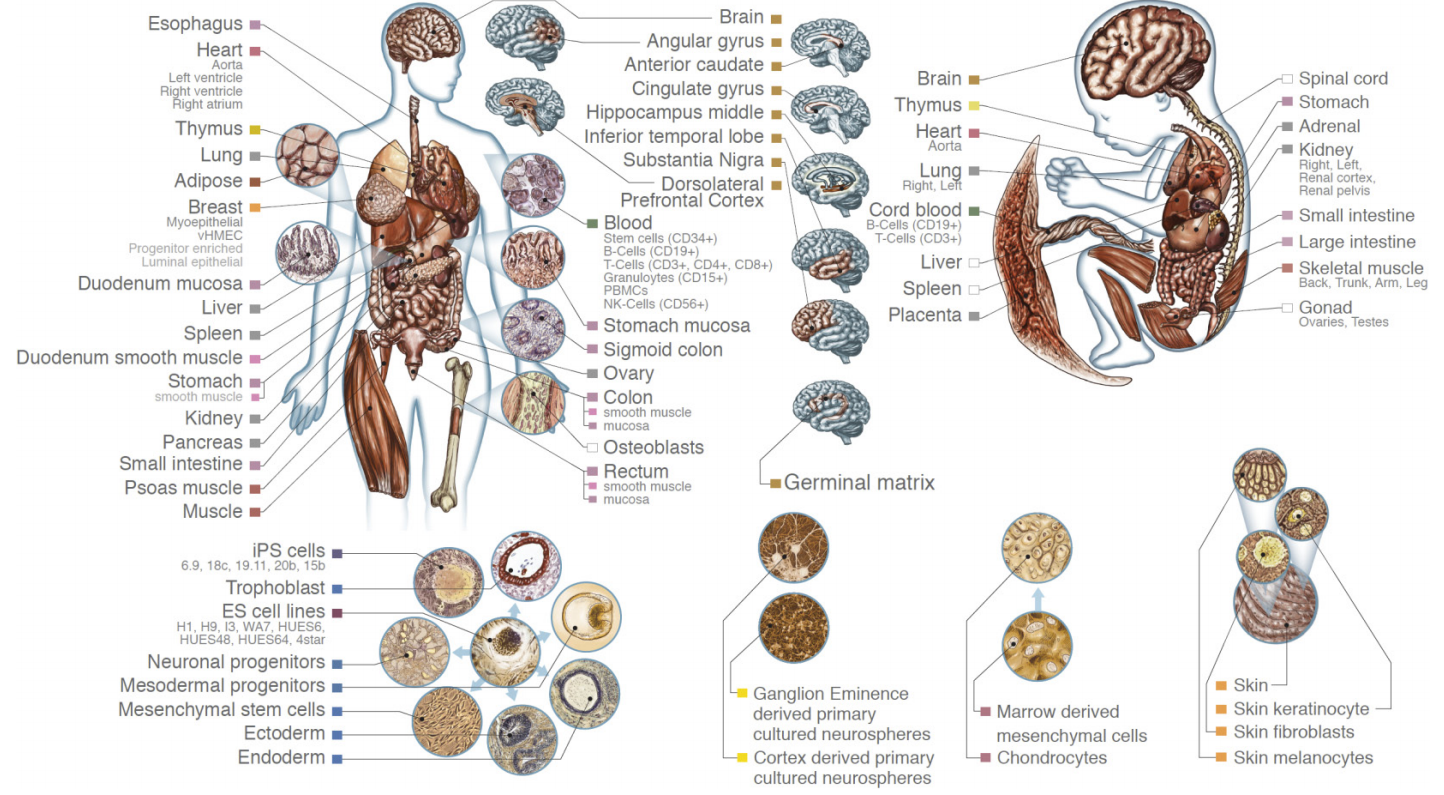
\includegraphics[width=0.85\linewidth]{slides/roadmap_tissues.png}
  \caption{Primary tissues and cell types profiled by the Roadmap Epigenomics project. Reproduced from \citet{roadmap2015}.}
  \label{fig:roadmap}
\end{figure}

Histone modifications are named by the histone (H3, H4, H2A, H2B), the modified amino acid residue (for example K4, lysine 4) and the modification (me1, me2 or me3 for mono-, di- or trimethylation; ac for acetylation). So H3K4me3 is trimethylation of lysine 4 on histone H3. Data from one tissue look like a set of tracks along the genome (Figure~\ref{fig:capza2}). Each track is the ChIP-seq read coverage for one modification, or for another chromatin protein: RNA polymerase II (Pol II), the enzyme that transcribes DNA into RNA, so that its presence indicates active transcription; CTCF, which together with cohesin controls chromatin looping and so which regulatory elements can contact which genes; and the histone variant H2A.Z. The window shown is about 100 kb around the gene \textit{CAPZA2}, a tiny fraction of the 3 billion nucleotide genome, and it is already hard to take in by eye.

\begin{figure}[tbp]
  \centering
  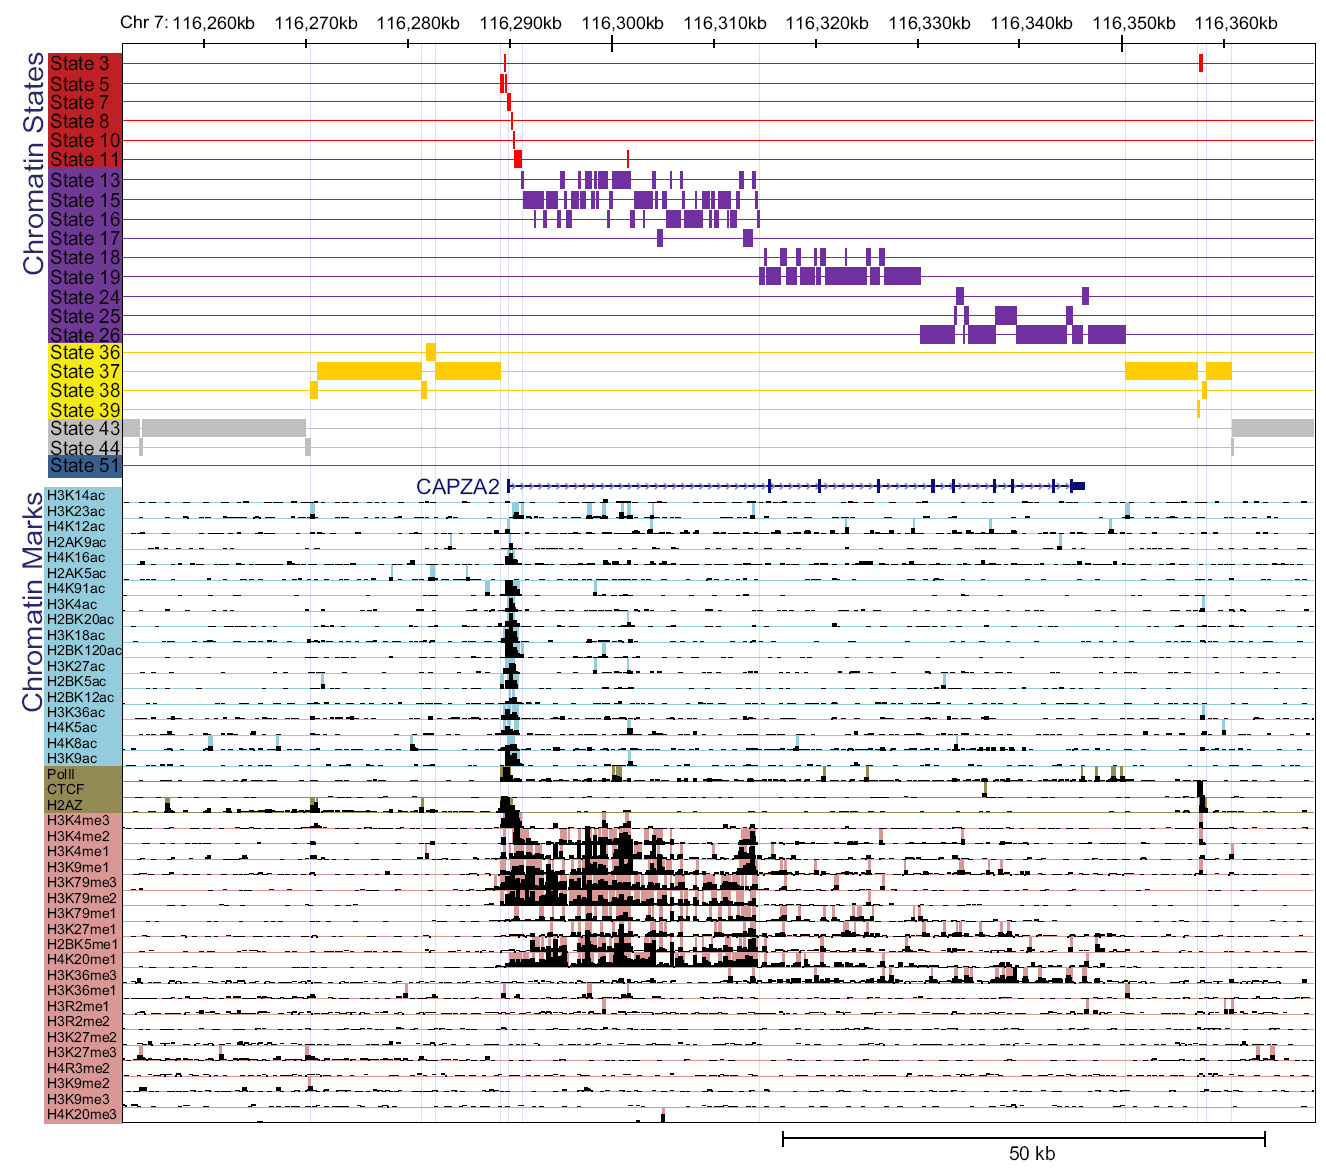
\includegraphics[width=0.8\linewidth]{slides/capza2_states.png}
  \caption{About 100 kb of chromosome 7 around the gene \textit{CAPZA2} in human CD4$^+$ T cells. Bottom, ChIP-seq signal for 38 histone modifications, Pol II, CTCF and H2A.Z, grouped into acetylations (blue) and methylations (pink). Middle, the \textit{CAPZA2} gene. Top, chromatin states learned by an HMM with 51 states, one row per state. The promoter states (red) sit at the transcription start site and the transcribed states (purple) cover the gene body. The gene annotation was not used to learn the states. Reproduced from \citet{ernst2010}, using data from \citet{barski2007} and \citet{wang2008}.}
  \label{fig:capza2}
\end{figure}

\subsection{Types of genomic region}

Combinations of chromatin marks distinguish several types of region (Figure~\ref{fig:chromatin_cartoon}).
\begin{itemize}
  \item \emph{Promoters} lie immediately upstream of a gene's transcription start site (TSS). Transcription factors bind there and recruit Pol II. Active promoters carry H3K4me3, along with H3K27ac and H3K9ac, and are accessible.
  \item \emph{Enhancers} also bind transcription factors and increase transcription, but lie further from the gene they regulate, at least thousands and up to hundreds of thousands of nucleotides away along the linear sequence. To act they must come close to the promoter in three dimensions, through chromatin looping. Promoters and enhancers are more alike than different. The main distinction is distance from the gene, but there is also a difference in marks: H3K4me1 is stronger at enhancers than at promoters, and H3K4me3 is stronger at promoters. H3K27ac marks both when active.
  \item \emph{Transcribed regions} are the bodies of genes being expressed in the cell type. They carry H3K36me3, which is deposited as Pol II moves along the gene, and H4K20me1 and H3K79me2.
  \item \emph{Repressed regions} are not transcribed. Polycomb-repressed regions carry H3K27me3. Constitutive heterochromatin carries H3K9me3. Repressed chromatin is typically compacted and less accessible.
  \item \emph{Poised} or bivalent regions carry both an activating mark (H3K4me3 or H3K4me1) and the repressive H3K27me3. They are not active but are ready to be: during development, a poised gene may be switched on at the next stage; in immune cells, a gene may be poised to respond to a stimulus.
  \item \emph{Insulators} block communication between neighbouring parts of the genome. They are bound by CTCF and often lie at the boundaries of topologically associating domains (TADs), the regions of frequent three-dimensional contact revealed by Hi-C (Chapter 3).
\end{itemize}

\begin{figure}[tbp]
  \centering
  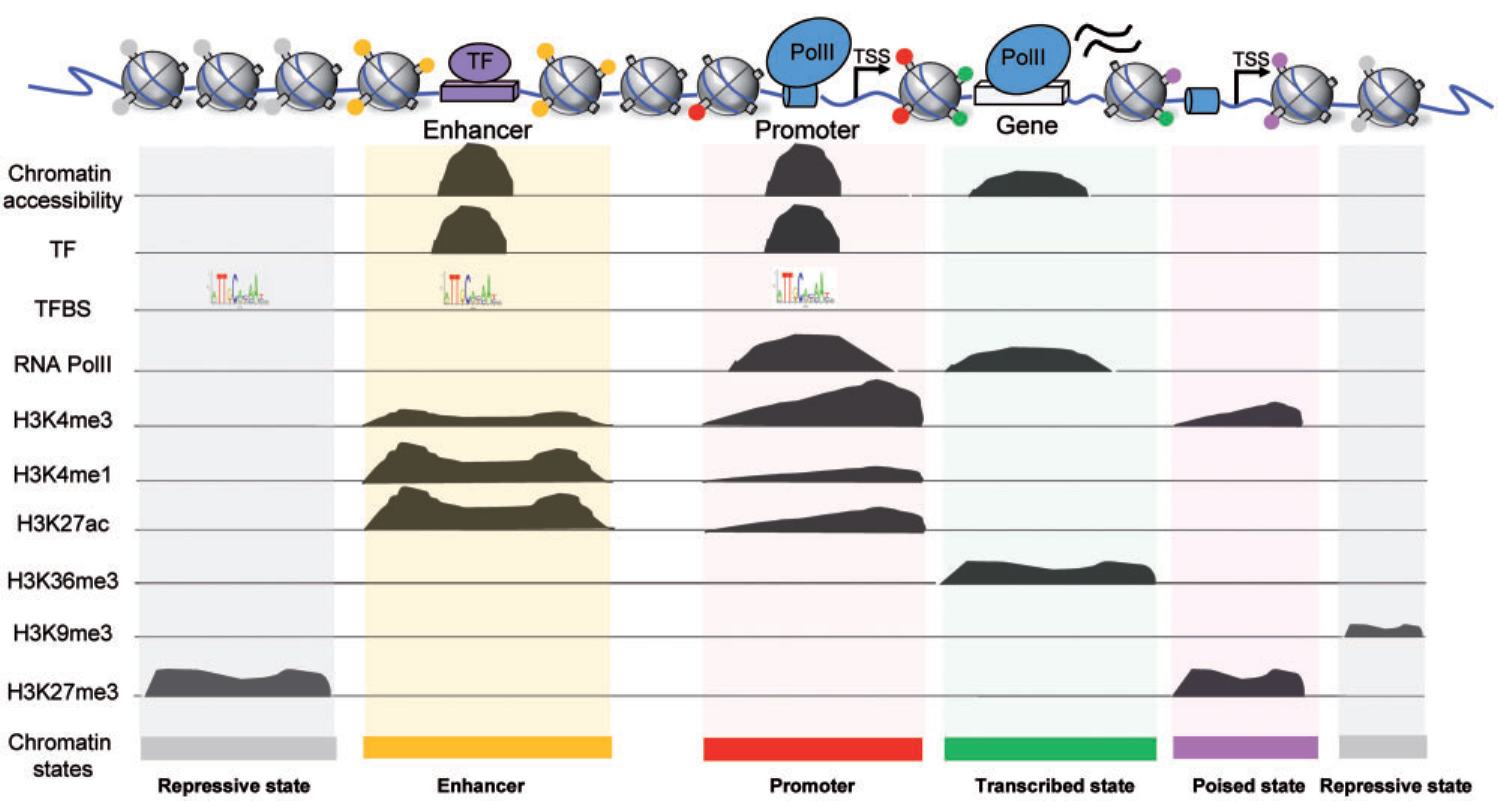
\includegraphics[width=0.85\linewidth]{slides/chromatin_state_cartoon.pdf}
  \caption{Schematic of chromatin signals that distinguish types of genomic region. Top, nucleosomes (grey), transcription factors (TF) and Pol II along DNA. Tracks show chromatin accessibility, TF binding and binding sites (TFBS), Pol II, and six histone modifications. Bottom, the chromatin state each combination defines. \textbf{[Source to be confirmed.]}}
  \label{fig:chromatin_cartoon}
\end{figure}

There are dozens of histone modifications, which can act alone or in combination, so the number of possible combinations is astronomical. Rather than define region types by hand from prior knowledge, we would like to learn the biologically meaningful combinations from their genome-wide co-occurrence. These combinations, together with their spatial context along the genome, define \emph{chromatin states}, which can then be interpreted as promoters, enhancers, transcribed regions and so on. A chromatin state annotation can be used to annotate the genome systematically and, when learned across cell types, to study how chromatin changes between them.

%======================================================================
\section{ChromHMM: setting up the data}
\label{sec:chromhmm_data}
%======================================================================

ChromHMM~\citep{ernst2010,ernst2012} prepares the data in two steps.
\begin{enumerate}
  \item \emph{Binning.} The genome is divided into non-overlapping windows of 200 bp (the default bin size), and the reads of each ChIP-seq experiment are counted in each bin. For the human genome this gives about $3\times 10^9/200 = 1.5\times 10^7$ bins.
  \item \emph{Binarization.} Each count is converted to 1 (mark present) or 0 (absent). The count is compared with a Poisson background distribution whose rate is the average count per bin for that experiment, or is set from a control (input) experiment, and the bin is called present if the count is significantly higher than expected from the background (by default, a Poisson upper-tail $p$-value below $10^{-4}$).
\end{enumerate}
The result is a binary matrix $\mY\in\{0,1\}^{S\times M}$, where $S$ is the number of bins and $M$ the number of marks. Entry $y_{tm}$ is 1 if mark $m\in\{1,\dots,M\}$ is present in bin $t\in\{1,\dots,S\}$, and row $t$ is the vector $\vy_t^\top$, with $\vy_t\in\{0,1\}^M$. Binarization discards information about signal strength, but it makes the model robust to differences in sequencing depth and signal-to-noise between experiments.

We could cluster the $1.5\times 10^7$ vectors $\vy_t$ with any method from Chapter 5, for example a mixture of multivariate Bernoulli distributions. A clustering model treats the bins as independent and ignores their order. But there is structure in how region types follow each other along the genome. If bin $t$ is in a gene body, bin $t+1$ is most likely in the gene body too, since genes are typically thousands of nucleotides long. If bin $t$ is an active promoter, the next bins in the direction of transcription are likely to be transcribed. An HMM uses this structure to smooth the cluster assignments along the genome, which helps because the data are noisy: a single bin may lack a mark by chance even inside a region where the mark is present.

Figure~\ref{fig:chromhmm_toy} shows the idea on a toy example. Each bin has a hidden state, which we do not observe. Each state has a characteristic probability of showing each mark, and consecutive states follow a pattern: an enhancer state, then promoter states at the TSS, then transcribed states along the gene, then a state with no marks. After fitting, states are interpreted by looking at which marks they emit.

\begin{figure}[tbp]
  \centering
  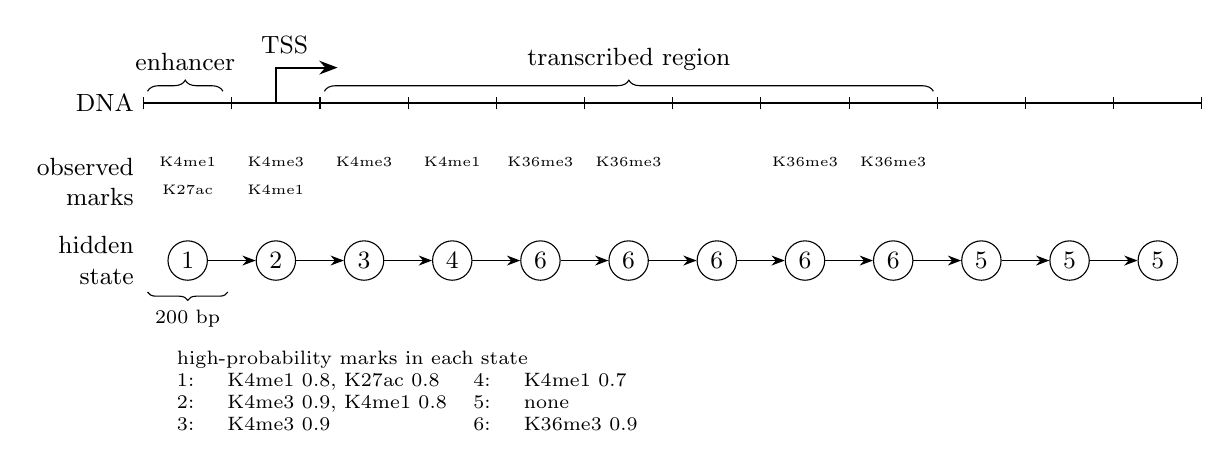
\begin{tikzpicture}[>=Stealth, every node/.style={font=\small}]
    \def\w{1.12}
    % DNA and annotation
    \draw[thick] (0,0) -- (12*\w,0);
    \node[left] at (0,0) {DNA};
    \draw[decorate, decoration={brace, amplitude=4pt}] (0.05,0.15) -- (0.9*\w,0.15) node[midway, above=4pt] {enhancer};
    \draw[->, thick] (1.5*\w,0) -- (1.5*\w,0.45) -- (2.2*\w,0.45);
    \node[above] at (1.6*\w,0.5) {TSS};
    \draw[decorate, decoration={brace, amplitude=4pt}] (2.05*\w,0.15) -- (9*\w-0.05,0.15) node[midway, above=4pt] {transcribed region};
    \foreach \i in {0,...,12} \draw (\i*\w,-0.08) -- (\i*\w,0.08);
    % observed marks
    \node[left, align=right] at (0,-1.0) {observed\\marks};
    \foreach \i/\a/\b in {0/K4me1/K27ac, 1/K4me3/K4me1, 2/K4me3/, 3/K4me1/, 4/K36me3/, 5/K36me3/, 6//, 7/K36me3/, 8/K36me3/} {
      \node[font=\tiny] at (\i*\w+0.5*\w,-0.75) {\a};
      \node[font=\tiny] at (\i*\w+0.5*\w,-1.1) {\b};
    }
    % hidden states
    \node[left, align=right] at (0,-2.0) {hidden\\state};
    \foreach \i/\s in {0/1,1/2,2/3,3/4,4/6,5/6,6/6,7/6,8/6,9/5,10/5,11/5} {
      \node[draw, circle, inner sep=1.5pt, minimum size=0.5cm] (h\i) at (\i*\w+0.5*\w,-2.0) {\s};
    }
    \foreach \i [evaluate=\i as \j using int(\i+1)] in {0,...,10} \draw[->] (h\i) -- (h\j);
    \draw[decorate, decoration={brace, mirror, amplitude=3pt}] (0.05,-2.4) -- (\w-0.05,-2.4) node[midway, below=3pt, font=\scriptsize] {200 bp};
    % emission table
    \node[anchor=north west, align=left, font=\scriptsize] at (0.3,-3.0) {%
      \begin{tabular}{@{}cl@{\hspace{1.2em}}cl@{}}
        \multicolumn{4}{@{}l}{high-probability marks in each state}\\
        1: & K4me1 0.8, K27ac 0.8 & 4: & K4me1 0.7 \\
        2: & K4me3 0.9, K4me1 0.8 & 5: & none \\
        3: & K4me3 0.9 & 6: & K36me3 0.9
      \end{tabular}};
  \end{tikzpicture}
  \caption{A toy chromatin state model, adapted from a teaching diagram by the ChromHMM authors. The genome is split into 200 bp bins. Each bin has an unobserved state (circles), and each state emits each histone mark (H3 prefix dropped) with a state-specific probability (bottom). The hidden states follow each other along the genome: enhancer (1), promoter flanks and TSS (2--4), transcribed (6), no signal (5). In bin 7 the transcribed state is inferred although no mark is observed, because of its neighbours. All probabilities are learned from the chromatin data alone.}
  \label{fig:chromhmm_toy}
\end{figure}

%======================================================================
\section{Conditional independence and graphical models}
\label{sec:pgm}
%======================================================================

To write down the HMM precisely we need some background on probabilistic graphical models, which represent the dependencies among a set of random variables. The key concepts are independence and conditional independence.

\subsection{Independence and conditional independence}

Two random variables $A$ and $B$ are \emph{independent} if knowing $A$ tells us nothing about $B$, and vice versa. Formally, $P(A\mid B)=P(A)$ for all values of $A$ and $B$. Substituting into the product rule $P(A,B)=P(A\mid B)P(B)$ gives
\begin{equation}
  P(A,B) = P(A)\,P(B),
\end{equation}
so the joint distribution is the product of the marginals. We write $A\indep B$. The relation is symmetric: $P(A,B)=P(A)P(B)$ also implies $P(B\mid A)=P(B)$.

$A$ and $B$ are \emph{conditionally independent} given a third variable $C$ if, once we know $C$, $A$ tells us nothing more about $B$,
\begin{equation}
  P(A\mid B,C) = P(A\mid C),
\end{equation}
or equivalently, by the product rule,
\begin{equation}
  P(A,B\mid C) = P(A\mid B,C)\,P(B\mid C) = P(A\mid C)\,P(B\mid C).
\end{equation}
We write $A\indep B\mid C$, which is the same statement as $B\indep A\mid C$.

\subsection{Directed graphical models}

A directed graphical model, or Bayesian network~\citep{pearl1988,koller2009}, represents a joint distribution over random variables $X_1,\dots,X_N$ by a directed acyclic graph with one node per variable. The joint distribution factorizes as a product of one term per variable, the conditional distribution of that variable given its parents in the graph,
\begin{equation}
  P(X_1,\dots,X_N) = \prod_{n=1}^N P\left(X_n \mid \operatorname{pa}(X_n)\right),
  \label{eq:dag_factorization}
\end{equation}
where $\operatorname{pa}(X_n)$ is the set of parents of $X_n$. For the graph in Figure~\ref{fig:dag}a,
\begin{equation}
  P(X_1,X_2,X_3,X_4) = P(X_1)\,P(X_2)\,P(X_3\mid X_1,X_2)\,P(X_4\mid X_3).
\end{equation}
Missing edges encode independence assumptions. Here $X_1$ and $X_2$ have no parents and are independent, and $X_4$ depends on $X_1$ and $X_2$ only through $X_3$, so $X_4\indep(X_1,X_2)\mid X_3$. (``Graph'' here means a network, not a plot.) In the early 2000s there was much interest in learning the graph structure itself from data, for example from gene expression or clinical records. Structure learning is hard in general and we will not attempt it. We use graphs as a compact way to write down models such as the HMM.

\begin{figure}[tbp]
  \centering
  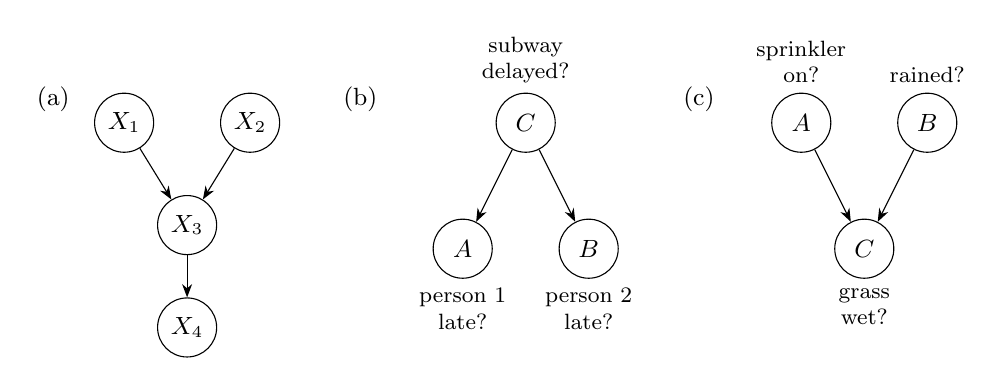
\begin{tikzpicture}[>=Stealth, node distance=1.1cm, every node/.style={font=\small},
      var/.style={draw, circle, minimum size=0.75cm, inner sep=0pt}]
    % (a) toy DAG
    \node at (-0.9,1.3) {(a)};
    \node[var] (x1) at (0,1) {$X_1$};
    \node[var] (x2) at (1.6,1) {$X_2$};
    \node[var] (x3) at (0.8,-0.3) {$X_3$};
    \node[var] (x4) at (0.8,-1.6) {$X_4$};
    \draw[->] (x1) -- (x3); \draw[->] (x2) -- (x3); \draw[->] (x3) -- (x4);
    % (b) confounder
    \begin{scope}[xshift=4.3cm]
      \node at (-1.3,1.3) {(b)};
      \node[var] (c) at (0.8,1) {$C$};
      \node[var] (a) at (0,-0.6) {$A$};
      \node[var] (b) at (1.6,-0.6) {$B$};
      \draw[->] (c) -- (a); \draw[->] (c) -- (b);
      \node[above, align=center, font=\footnotesize] at (c.north) {subway\\delayed?};
      \node[below, align=center, font=\footnotesize] at (a.south) {person 1\\late?};
      \node[below, align=center, font=\footnotesize] at (b.south) {person 2\\late?};
    \end{scope}
    % (c) collider
    \begin{scope}[xshift=8.6cm]
      \node at (-1.3,1.3) {(c)};
      \node[var] (a) at (0,1) {$A$};
      \node[var] (b) at (1.6,1) {$B$};
      \node[var] (c) at (0.8,-0.6) {$C$};
      \draw[->] (a) -- (c); \draw[->] (b) -- (c);
      \node[above, align=center, font=\footnotesize] at (a.north) {sprinkler\\on?};
      \node[above, align=center, font=\footnotesize] at (b.north) {rained?};
      \node[below, align=center, font=\footnotesize] at (c.south) {grass\\wet?};
    \end{scope}
  \end{tikzpicture}
  \caption{Directed graphical models. (a) A toy graph whose joint distribution factorizes as $P(X_1)P(X_2)P(X_3\mid X_1,X_2)P(X_4\mid X_3)$. (b) A common cause (confounder): $A$ and $B$ are dependent but conditionally independent given $C$. (c) A collider: $A$ and $B$ are independent but become dependent given $C$.}
  \label{fig:dag}
\end{figure}

\subsection{Dependent but conditionally independent: confounders}

Suppose we are hosting a dinner, $A$ is whether one guest is late and $B$ is whether another guest is late. Both travel by subway, and $C$ is whether the subway is delayed (Figure~\ref{fig:dag}b). The graph gives
\begin{equation}
  P(A,B,C) = P(A\mid C)\,P(B\mid C)\,P(C).
\end{equation}
Conditioning on $C$,
\begin{equation}
  P(A,B\mid C) = \frac{P(A,B,C)}{P(C)} = P(A\mid C)\,P(B\mid C),
\end{equation}
so $A\indep B\mid C$. Marginally, however,
\begin{equation}
  P(A,B) = \sum_C P(A\mid C)\,P(B\mid C)\,P(C),
\end{equation}
which in general does not equal $P(A)P(B)=\left[\sum_C P(A\mid C)P(C)\right]\left[\sum_C P(B\mid C)P(C)\right]$, so $A$ and $B$ are not independent. If we know nothing about the subway and learn that the first guest is late, it becomes more likely that the subway is delayed, and so more likely that the second guest is late too. But if we have already checked that the subway is delayed, the first guest's text adds nothing about the second guest. The common cause $C$ is a \emph{confounder}.

\subsection{Independent but not conditionally independent: explaining away}

Now let $A$ be whether a sprinkler, set on a timer with no rain sensor, ran last night, $B$ whether it rained last night, and $C$ whether the grass is wet in the morning (Figure~\ref{fig:dag}c). The joint distribution is
\begin{equation}
  P(A,B,C) = P(A)\,P(B)\,P(C\mid A,B).
\end{equation}
Summing over $C$,
\begin{equation}
  P(A,B) = \sum_C P(A)\,P(B)\,P(C\mid A,B) = P(A)\,P(B)\underbrace{\sum_C P(C\mid A,B)}_{=1} = P(A)\,P(B),
\end{equation}
so $A\indep B$: the sprinkler timer knows nothing about the weather. Conditioning on $C$,
\begin{equation}
  P(A,B\mid C) = \frac{P(A)\,P(B)\,P(C\mid A,B)}{P(C)},
\end{equation}
which in general does not factorize as $P(A\mid C)P(B\mid C)$, because $P(C\mid A,B)$ couples $A$ and $B$. A node with two incoming arrows is called a \emph{collider}. Observing it makes its parents dependent.

A numerical example shows the effect. Let $P(A=1)=0.5$ and $P(B=1)=0.2$, and let the grass be wet with probability 0 if neither cause occurred, 0.9 if exactly one did and 0.99 if both did. Then
\begin{align}
  P(C=1) &= 0.5\cdot 0.8\cdot 0.9 + 0.5\cdot 0.2\cdot 0.9 + 0.5\cdot 0.2\cdot 0.99 \nonumber\\ &= 0.36+0.09+0.099 = 0.549, \nonumber\\
  P(B=1\mid C=1) &= \frac{0.09+0.099}{0.549} = 0.34, \nonumber\\
  P(B=1\mid C=1, A=1) &= \frac{0.099}{0.36+0.099} = 0.22, \nonumber\\
  P(B=1\mid C=1, A=0) &= \frac{0.09}{0.09} = 1 .
\end{align}
Seeing wet grass raises the probability of rain from 0.2 to 0.34. Learning that the sprinkler ran lowers it again to 0.22, because the sprinkler already explains the wet grass; learning that the sprinkler did not run makes rain certain. The two causes compete to explain the observation, a phenomenon called \emph{explaining away}.

Explaining away is one of the central intuitions of graphical models, and we have met it before. In linear regression (Chapter 1) the coefficients are independent under the prior, but once we observe the response $\vy$ they become dependent. If two features are highly correlated, either could account for the signal in $\vy$, like rain and the sprinkler, and the posterior is uncertain about how much weight to put on each: the elongated likelihood contours of Chapter 1's colinearity example are explaining away between $\beta_1$ and $\beta_2$.

%======================================================================
\section{The hidden Markov model}
\label{sec:hmm}
%======================================================================

\subsection{Generative process}

An HMM has a sequence of hidden states $X_1,\dots,X_S$, one per position, and a sequence of observations $Y_1,\dots,Y_S$. Each state takes one of $K$ values, $X_t\in\{1,\dots,K\}$. The states form a Markov chain: $X_t$ depends on the past only through $X_{t-1}$. Each observation $Y_t$ depends only on the state $X_t$ at the same position (Figure~\ref{fig:hmm_graph}). The hidden states are \emph{latent variables}, variables in the model that we never observe, and models built this way are called latent variable models.

\begin{figure}[tbp]
  \centering
  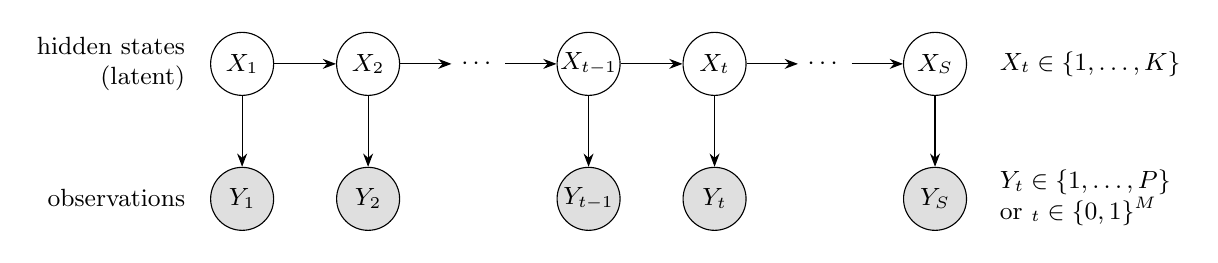
\begin{tikzpicture}[>=Stealth, every node/.style={font=\small},
      var/.style={draw, circle, minimum size=0.8cm, inner sep=0pt},
      obs/.style={draw, circle, minimum size=0.8cm, inner sep=0pt, fill=gray!25}]
    \node[var] (x1) at (0,0) {$X_1$};
    \node[var] (x2) at (1.6,0) {$X_2$};
    \node (d1) at (3.0,0) {$\cdots$};
    \node[var] (xtm) at (4.4,0) {$X_{t-1}$};
    \node[var] (xt) at (6.0,0) {$X_t$};
    \node (d2) at (7.4,0) {$\cdots$};
    \node[var] (xs) at (8.8,0) {$X_S$};
    \foreach \n/\l in {x1/Y_1, x2/Y_2, xtm/Y_{t-1}, xt/Y_t, xs/Y_S}
      \node[obs, below=0.9cm of \n] (y\n) {$\l$};
    \foreach \n in {x1, x2, xtm, xt, xs} \draw[->] (\n) -- (y\n);
    \draw[->] (x1) -- node[above] {$\mT$} (x2);
    \draw[->] (x2) -- (d1); \draw[->] (d1) -- (xtm);
    \draw[->] (xtm) -- node[above] {$\mT$} (xt);
    \draw[->] (xt) -- (d2); \draw[->] (d2) -- (xs);
    \node[right=2pt] at ($(xt)!0.5!(yxt)$) {$\mE$};
    \node[left, align=right] at (-0.6,0) {hidden states\\(latent)};
    \node[left, align=right] at (-0.6,-1.7) {observations};
    \node[right, align=left] at (9.5,0) {$X_t\in\{1,\dots,K\}$};
    \node[right, align=left] at (9.5,-1.7) {$Y_t\in\{1,\dots,P\}$\\or $\vy_t\in\{0,1\}^M$};
  \end{tikzpicture}
  \caption{The hidden Markov model as a directed graphical model. Hidden states (white) form a Markov chain governed by the transition matrix $\mT$; each observation (shaded) depends only on the hidden state at the same position, through the emission matrix $\mE$.}
  \label{fig:hmm_graph}
\end{figure}

The model has three sets of parameters.
\begin{itemize}
  \item The \emph{initial distribution} $\vpi\in\R^K$, with $\pi_i=P(X_1=i)$, $\pi_i\geq 0$ and $\sum_i\pi_i=1$.
  \item The \emph{transition matrix} $\mT\in\R^{K\times K}$, with
  \begin{equation}
    T_{ij} = P(X_t=j\mid X_{t-1}=i),
  \end{equation}
  the probability of moving from state $i$ at position $t-1$ to state $j$ at position $t$. Each row is a probability distribution, $T_{ij}\geq 0$ and $\sum_j T_{ij}=1$. The same matrix is used at every position, so the chain is \emph{homogeneous}.
  \item The \emph{emission} parameters, which give the distribution of an observation given the state. In the simplest case the observation is categorical, $Y_t\in\{1,\dots,P\}$, and the emission matrix $\mE\in\R^{K\times P}$ has entries
  \begin{equation}
    E_{ij} = P(Y_t=j\mid X_t=i),
  \end{equation}
  with $E_{ij}\geq 0$ and $\sum_j E_{ij}=1$. Row $i$ is the distribution of observations in state $i$.
\end{itemize}
We collect the parameters as $\vtheta=(\vpi,\mT,\mE)$. The generative process is: draw $X_1\sim\text{Categorical}(\vpi)$; for $t=2,\dots,S$ draw $X_t\mid X_{t-1}\sim\text{Categorical}(\mT_{X_{t-1},:})$, the row of $\mT$ for the previous state; and for each $t$ draw $Y_t\mid X_t\sim\text{Categorical}(\mE_{X_t,:})$.

\subsection{The joint distribution}

Applying the factorization~\eqref{eq:dag_factorization} to the graph in Figure~\ref{fig:hmm_graph}, the joint probability of a state sequence $x=(x_1,\dots,x_S)$ and observations $Y=(y_1,\dots,y_S)$ is
\begin{equation}
  P(x,Y\mid\vtheta) = P(x_1)\,P(y_1\mid x_1)\prod_{t=2}^S P(x_t\mid x_{t-1})\,P(y_t\mid x_t)
  = \pi_{x_1}E_{x_1y_1}\prod_{t=2}^S T_{x_{t-1}x_t}E_{x_ty_t}.
  \label{eq:hmm_joint}
\end{equation}
We use lower case $x_t$ for a particular value of the random variable $X_t$. It will be convenient to write the emission term at position $t$ as a function of the state,
\begin{equation}
  \phi_t(i) = P(y_t\mid X_t=i),
\end{equation}
and $\vphi_t\in\R^K$ for the vector of these values. For categorical emissions $\phi_t(i)=E_{iy_t}$, column $y_t$ of $\mE$. The observations are fixed, so $\vphi_t$ is a known vector once $\mE$ is given.

The graph encodes the conditional independence properties that make the HMM tractable:
\begin{itemize}
  \item given $X_t$, the future states and observations $(X_{t+1:S},Y_{t+1:S})$ are independent of the past $(X_{1:t-1},Y_{1:t})$;
  \item given $X_t$, the observation $Y_t$ is independent of everything else.
\end{itemize}
Here $Y_{a:b}$ denotes $(Y_a,\dots,Y_b)$. Note that the observations are \emph{not} independent of each other marginally: $Y_1$ and $Y_2$ are dependent through $X_1$ and $X_2$. This is what allows neighbouring bins to inform each other.

\subsection{Emissions for chromatin data}

In ChromHMM the observation at bin $t$ is a binary vector $\vy_t\in\{0,1\}^M$ over $M$ marks, not a single category. Treating each of the $2^M$ combinations as a category would need $K(2^M-1)$ emission parameters. Instead ChromHMM assumes that the marks are conditionally independent given the state, each Bernoulli,
\begin{equation}
  \phi_t(i) = P(\vy_t\mid X_t=i) = \prod_{m=1}^M E_{im}^{y_{tm}}\left(1-E_{im}\right)^{1-y_{tm}},
  \label{eq:bernoulli_emission}
\end{equation}
where now $\mE\in[0,1]^{K\times M}$ and $E_{im}=P(y_{tm}=1\mid X_t=i)$ is the probability of observing mark $m$ in state $i$. The rows of this $\mE$ need not sum to one. Marks are correlated across the genome, but in this model only through the state: a promoter state has high probability of both H3K4me3 and H3K27ac. All the algorithms below use the emissions only through $\vphi_t$, so they apply unchanged to any emission model, including Gaussian or Poisson emissions for continuous or count data.

\subsection{An HMM is a mixture model with dependencies}

If every row of $\mT$ equals $\vpi$, then $P(X_t=j\mid X_{t-1}=i)=\pi_j$ regardless of $i$, the states are independent, and the HMM reduces to a mixture model with mixture weights $\vpi$ and component distributions given by the rows of $\mE$. The emission parameters play the role of the cluster centres. The HMM's new ingredient is the transition matrix, which says how likely we are, before seeing any data, to move from one state to another between consecutive bins.

A large diagonal entry $T_{ii}$ means state $i$ tends to persist. The number of consecutive bins $L$ spent in state $i$ before leaving has a geometric distribution,
\begin{equation}
  P(L=\ell) = T_{ii}^{\ell-1}\left(1-T_{ii}\right), \qquad \E[L] = \frac{1}{1-T_{ii}},
\end{equation}
since we stay $\ell-1$ times and then leave (Figure~\ref{fig:dwell}). With 200 bp bins, $T_{ii}=0.99$ gives segments of 100 bins, or 20 kb, on average, the scale of a gene body, while $T_{ii}=0.8$ gives segments of about 1 kb, the scale of a promoter. The geometric distribution always has its mode at $\ell=1$; models that need other segment length distributions can use several states with the same emissions in series, or a hidden semi-Markov model.

\begin{figure}[tbp]
  \centering
  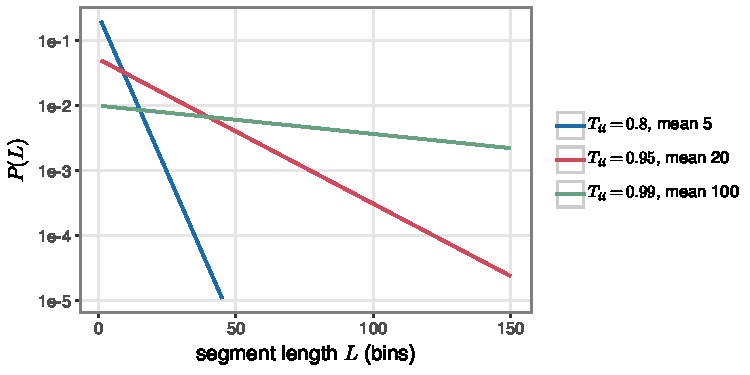
\includegraphics[width=0.7\linewidth]{dwell_time.pdf}
  \caption{Distribution of the number of consecutive bins spent in a state with self-transition probability $T_{ii}$. The distribution is geometric with mean $1/(1-T_{ii})$, so it is a straight line on a log scale.}
  \label{fig:dwell}
\end{figure}

%======================================================================
\section{Inference: the forward-backward algorithm}
\label{sec:fb}
%======================================================================

\subsection{What we need to compute}

We observe $Y$ but not the states $X$, and we do not know the parameters $\mT$ and $\mE$. As for $K$-means and mixture models in Chapter 5, we will fit the model by alternating between estimating the states given the parameters and estimating the parameters given the states. The first step requires the posterior distribution of the states given the data, $P(X\mid Y,\vtheta)$. Specifically, we need the \emph{posterior marginal} of each state,
\begin{equation}
\begin{split}
  \gamma_t(i) = P(X_t=i\mid Y,\vtheta) = \sum_{x_1=1}^K\cdots\sum_{x_{t-1}=1}^K\;\sum_{x_{t+1}=1}^K\cdots\sum_{x_S=1}^K &P(x_1,\dots,x_{t-1},X_t=i,\\
  &\quad x_{t+1},\dots,x_S\mid Y,\vtheta),
\end{split}
  \label{eq:marginal_naive}
\end{equation}
which sums the joint posterior over all values of every state except $X_t$. For example, with $S=3$, $P(X_2\mid Y)=\sum_{x_1}\sum_{x_3}P(x_1,X_2,x_3\mid Y)$. The marginal $\vgamma_t\in\R^K$ is a soft assignment of bin $t$ to the states, like the responsibilities of a mixture model.

Evaluated directly,~\eqref{eq:marginal_naive} has $K^{S-1}$ terms. With $K=15$ states and $S=1.5\times 10^7$ bins this is hopeless, and even $K=2$, $S=100$ gives $2^{99}\approx 6\times 10^{29}$ terms. The forward-backward algorithm computes all the marginals $\vgamma_1,\dots,\vgamma_S$ in $O(SK^2)$ operations by exploiting the chain structure of the graph. It is an instance of \emph{belief propagation}~\citep{pearl1988}, a general class of algorithms for computing marginals in graphical models, which is in turn an instance of dynamic programming.

\subsection{Why the chain structure helps}

The saving comes from the distributive law, $ab+ac=a(b+c)$: factor out terms that do not depend on the summation variable before summing. Consider the probability of the data, $P(Y\mid\vtheta)=\sum_x P(x,Y\mid\vtheta)$. Using~\eqref{eq:hmm_joint} and moving each sum as far right as it can go,
\begin{equation}
  P(Y) = \sum_{x_S}\phi_S(x_S)\sum_{x_{S-1}}T_{x_{S-1}x_S}\,\phi_{S-1}(x_{S-1})\cdots\sum_{x_2}T_{x_2x_3}\,\phi_2(x_2)\sum_{x_1}T_{x_1x_2}\,\phi_1(x_1)\,\pi_{x_1}.
\end{equation}
The innermost sum over $x_1$ gives a function of $x_2$ only, a vector of length $K$, at a cost of $K^2$ operations. Multiplying by $\phi_2(x_2)$ and summing over $x_2$ gives a function of $x_3$, and so on. Each step costs $K^2$, so the total is $O(SK^2)$ instead of $O(K^S)$. The vectors passed from one sum to the next are the forward messages. Running the same idea from the other end of the chain gives the backward messages, and combining the two gives every marginal.

\subsection{Forward pass}

Define, for $t=1,\dots,S$ and $i=1,\dots,K$,
\begin{align}
  r_t(i) &= P(X_t=i\mid y_{1:t-1}) && \text{(predicted: state at $t$ given data before $t$)},\\
  f_t(i) &= P(X_t=i\mid y_{1:t}) && \text{(filtered: state at $t$ given data up to $t$)},\\
  c_t &= P(y_t\mid y_{1:t-1}) && \text{(normalizer)},
\end{align}
with $y_{1:0}$ empty, and write $\vr_t,\vf_t\in\R^K$ for the vectors. We suppress the conditioning on $\vtheta$. The recursion has two steps. Initially $\vr_1=\vpi$.

\emph{Update with the observation.} By Bayes' rule, and because $y_t\indep y_{1:t-1}\mid X_t$,
\begin{equation}
  f_t(i) = \frac{P(y_t\mid X_t=i, y_{1:t-1})\,P(X_t=i\mid y_{1:t-1})}{P(y_t\mid y_{1:t-1})} = \frac{\phi_t(i)\,r_t(i)}{c_t},
  \qquad c_t = \sum_{i=1}^K\phi_t(i)\,r_t(i).
\end{equation}
In vector form, $\vf_t=(\vr_t\odot\vphi_t)/c_t$, where $\odot$ is elementwise multiplication and $c_t=\vone^\top(\vr_t\odot\vphi_t)$ normalizes the vector to sum to one.

\emph{Predict the next state.} Summing over the current state, and because $X_{t+1}\indep y_{1:t}\mid X_t$,
\begin{equation}
  r_{t+1}(j) = \sum_{i=1}^K P(X_{t+1}=j\mid X_t=i)\,P(X_t=i\mid y_{1:t}) = \sum_{i=1}^K T_{ij}\,f_t(i),
  \qquad \vr_{t+1} = \mT^\top\vf_t .
\end{equation}
This is a matrix-vector product with dimensions $[K\times K][K\times 1]$, costing $K^2$ operations. Alternating the two steps from $t=1$ to $t=S$ is the forward pass.

As a by-product the forward pass gives the likelihood. By the chain rule of probability,
\begin{equation}
  P(Y\mid\vtheta) = \prod_{t=1}^S P(y_t\mid y_{1:t-1}) = \prod_{t=1}^S c_t,
  \qquad \log P(Y\mid\vtheta) = \sum_{t=1}^S\log c_t .
  \label{eq:hmm_loglik}
\end{equation}
Normalizing $\vf_t$ at each step is also what makes the computation numerically feasible: the unnormalized joint $P(X_t,y_{1:t})$ is a product of $t$ probabilities and underflows to zero for long sequences, while $\vf_t$ is a probability vector and the likelihood is accumulated on the log scale.

\subsection{Backward pass}

The forward pass uses only the data up to position $t$. To use the data after $t$, define
\begin{equation}
  b_t(i) = P(y_{t+1:S}\mid X_t=i),
\end{equation}
the probability of the future observations given the current state, with $b_S(i)=1$ since there are no future observations. Summing over the next state and using the conditional independence properties of the chain,
\begin{align}
  b_t(i) &= \sum_{j=1}^K P(X_{t+1}=j\mid X_t=i)\,P(y_{t+1}\mid X_{t+1}=j)\,P(y_{t+2:S}\mid X_{t+1}=j) \nonumber\\
  &= \sum_{j=1}^K T_{ij}\,\phi_{t+1}(j)\,b_{t+1}(j),
  \qquad \vbw_t = \mT\left(\vphi_{t+1}\odot\vbw_{t+1}\right).
\end{align}
Note that $\mT$ appears here without a transpose: the backward message travels against the direction of the arrows. Running from $t=S-1$ down to $t=1$ is the backward pass. Only the shape of $\vbw_t$ as a function of $i$ matters below, so it can be rescaled by any positive constant at each step to avoid underflow; dividing by $c_{t+1}$ is a common choice.

\subsection{Combining the messages}

The data split into the past and present, $y_{1:t}$, and the future, $y_{t+1:S}$, which are conditionally independent given $X_t$. Therefore
\begin{equation}
  \gamma_t(i) = P(X_t=i\mid Y) \propto P(X_t=i\mid y_{1:t})\,P(y_{t+1:S}\mid X_t=i) = f_t(i)\,b_t(i),
  \qquad \vgamma_t = \frac{\vf_t\odot\vbw_t}{\vone^\top(\vf_t\odot\vbw_t)} .
  \label{eq:gamma}
\end{equation}
The forward message summarizes everything the observations at and before $t$ say about $X_t$, the backward message summarizes everything the later observations say, and their product, normalized, is the posterior marginal (Figure~\ref{fig:fb_messages}). One forward pass and one backward pass give the marginals at every position.

\begin{figure}[tbp]
  \centering
  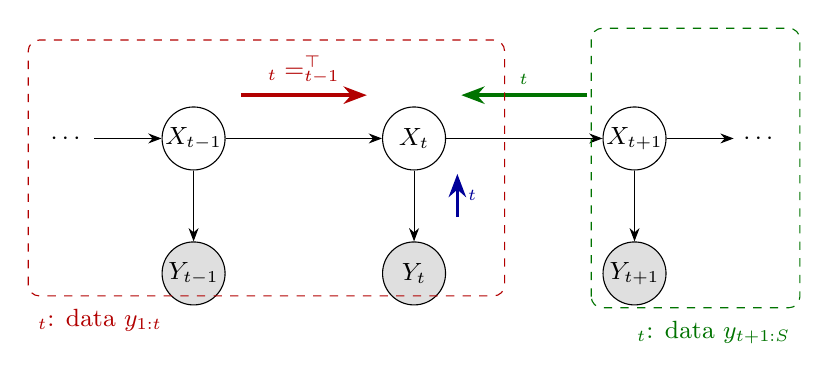
\begin{tikzpicture}[>=Stealth, every node/.style={font=\small},
      var/.style={draw, circle, minimum size=0.8cm, inner sep=0pt},
      obs/.style={draw, circle, minimum size=0.8cm, inner sep=0pt, fill=gray!25}]
    \node[var] (xa) at (0,0) {$X_{t-1}$};
    \node[var] (xt) at (2.8,0) {$X_t$};
    \node[var] (xb) at (5.6,0) {$X_{t+1}$};
    \node (l) at (-1.6,0) {$\cdots$};
    \node (r) at (7.2,0) {$\cdots$};
    \foreach \n/\lab in {xa/Y_{t-1}, xt/Y_t, xb/Y_{t+1}} \node[obs, below=0.9cm of \n] (y\n) {$\lab$};
    \foreach \n in {xa, xt, xb} \draw[->] (\n) -- (y\n);
    \draw[->] (l) -- (xa); \draw[->] (xa) -- (xt); \draw[->] (xt) -- (xb); \draw[->] (xb) -- (r);
    \draw[->, very thick, red!70!black] (0.6,0.55) -- (2.2,0.55) node[midway, above] {$\vr_t=\mT^\top\vf_{t-1}$};
    \draw[->, very thick, green!45!black] (5.0,0.55) -- (3.4,0.55) node[midway, above] {$\vbw_t$};
    \draw[->, very thick, blue!60!black] (3.35,-1.0) -- (3.35,-0.45) node[midway, right] {$\vphi_t$};
    \draw[dashed, red!70!black, rounded corners] (-2.1,-2.0) rectangle (3.95,1.25);
    \draw[dashed, green!45!black, rounded corners] (5.05,-2.15) rectangle (7.7,1.4);
    \node[red!70!black, anchor=north west] at (-2.1,-2.05) {$\vf_t$: data $y_{1:t}$};
    \node[green!45!black, anchor=north east] at (7.7,-2.2) {$\vbw_t$: data $y_{t+1:S}$};
  \end{tikzpicture}
  \caption{Forward and backward messages for position $t$. The forward message combines the prediction $\vr_t$ from the left with the local evidence $\vphi_t$ to give $\vf_t$, which summarizes $y_{1:t}$. The backward message $\vbw_t=\mT(\vphi_{t+1}\odot\vbw_{t+1})$ summarizes $y_{t+1:S}$. The posterior marginal is proportional to $\vf_t\odot\vbw_t$.}
  \label{fig:fb_messages}
\end{figure}

\subsection{Pairwise marginals}

Learning the transition matrix also requires the posterior probability of each pair of consecutive states. For $t=2,\dots,S$, by the same argument,
\begin{align}
  \xi_t(i,j) &= P(X_{t-1}=i,X_t=j\mid Y) \nonumber\\
  &\propto P(X_{t-1}=i\mid y_{1:t-1})\,P(X_t=j\mid X_{t-1}=i)\,P(y_t\mid X_t=j)\,P(y_{t+1:S}\mid X_t=j) \nonumber\\
  &= f_{t-1}(i)\,T_{ij}\,\phi_t(j)\,b_t(j),
  \label{eq:xi}
\end{align}
normalized so that $\sum_{i,j}\xi_t(i,j)=1$. In matrix form, $\xi_t\propto\mT\odot\left(\vf_{t-1}(\vphi_t\odot\vbw_t)^\top\right)$, a $K\times K$ matrix. Summing $\xi_t(i,j)$ over $j$ recovers $\gamma_{t-1}(i)$.

The complete procedure is Algorithm~\ref{alg:fb}. Its cost is $O(SK^2)$ time and $O(SK)$ memory, since the forward messages must be stored until the backward pass reaches them. \citet{rabiner1989} gives a classic tutorial treatment, and Chapter 13 of \citet{bishop2006} a textbook one.

\begin{algorithm}[tbp]
  \caption{Forward-backward algorithm}
  \label{alg:fb}
  \begin{algorithmic}[1]
    \Require initial distribution $\vpi$, transition matrix $\mT$, emission vectors $\vphi_1,\dots,\vphi_S$
    \State $\vr_1\gets\vpi$
    \For{$t=1,\dots,S$} \Comment{forward pass}
      \State $c_t\gets\vone^\top(\vr_t\odot\vphi_t)$; \quad $\vf_t\gets(\vr_t\odot\vphi_t)/c_t$
      \State $\vr_{t+1}\gets\mT^\top\vf_t$
    \EndFor
    \State $\vbw_S\gets\vone$
    \For{$t=S-1,\dots,1$} \Comment{backward pass}
      \State $\vbw_t\gets\mT(\vphi_{t+1}\odot\vbw_{t+1})/c_{t+1}$
    \EndFor
    \For{$t=1,\dots,S$}
      \State $\vgamma_t\gets\vf_t\odot\vbw_t$ \Comment{sums to one with this scaling}
      \State \textbf{if} $t\geq 2$: $\xi_t\gets\mT\odot\left(\vf_{t-1}(\vphi_t\odot\vbw_t)^\top\right)/c_t$
    \EndFor
    \State \Return $\vgamma_{1:S}$, $\xi_{2:S}$, $\log P(Y)=\sum_t\log c_t$
  \end{algorithmic}
\end{algorithm}

With the scaling in Algorithm~\ref{alg:fb}, $\vbw_t$ equals $P(y_{t+1:S}\mid X_t)/P(y_{t+1:S}\mid y_{1:t})$, and then $\vf_t\odot\vbw_t$ and $\xi_t$ are already normalized. To see this, note that $P(y_{t+1:S}\mid y_{1:t})=\prod_{u=t+1}^S c_u$, and the recursion divides by exactly these factors.

\subsection{Factor graphs and the sum-product algorithm}

Forward-backward is a special case of the \emph{sum-product} algorithm on factor graphs~\citep{kschischang2001}, which computes marginals for any distribution of the form
\begin{equation}
  P(x) = \frac{1}{Z}\prod_{a}g_a(x_{\mathcal{N}(a)}),
\end{equation}
where each \emph{factor} $g_a$ is a non-negative function of a subset $\mathcal{N}(a)$ of the variables and $Z$ normalizes. A factor graph is a bipartite graph with a node for each variable, a node for each factor, and an edge between a factor and each variable it depends on. Messages are functions of a single variable, passed along edges in both directions:
\begin{align}
  \text{variable to factor:}\quad & q_{n\to a}(x_n) = \prod_{a'\in\mathcal{N}(n)\setminus a} r_{a'\to n}(x_n), \\
  \text{factor to variable:}\quad & r_{a\to n}(x_n) = \sum_{x_{\mathcal{N}(a)\setminus n}} g_a(x_{\mathcal{N}(a)}) \prod_{n'\in\mathcal{N}(a)\setminus n} q_{n'\to a}(x_{n'}),
\end{align}
where $\mathcal{N}(n)$ is the set of factors that involve variable $n$. A variable with only one factor sends the message $q=1$; a factor with only one variable sends $r_{a\to n}(x_n)=g_a(x_n)$. The marginal of a variable is the normalized product of all its incoming messages, $P(x_n)\propto\prod_{a\in\mathcal{N}(n)}r_{a\to n}(x_n)$. On a graph without cycles (a tree) the result is exact, and every marginal is obtained by passing one message in each direction along every edge. Chapter 26 of \citet{mackay2003} is a readable introduction.

\begin{figure}[tbp]
  \centering
  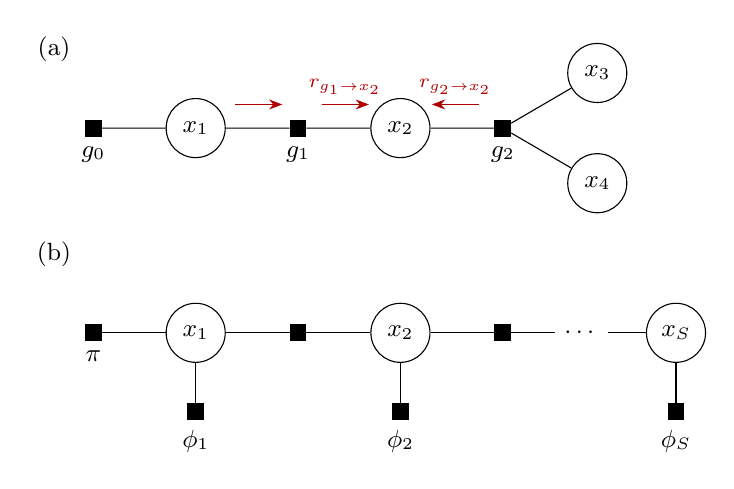
\begin{tikzpicture}[>=Stealth, every node/.style={font=\small},
      var/.style={draw, circle, minimum size=0.75cm, inner sep=0pt},
      fac/.style={draw, fill=black, minimum size=0.2cm, inner sep=0pt}]
    \node at (-1.3,1.0) {(a)};
    \node[fac, label=below:$g_0$] (f0) at (-0.8,0) {};
    \node[var] (x1) at (0.5,0) {$x_1$};
    \node[fac, label=below:$g_1$] (f1) at (1.8,0) {};
    \node[var] (x2) at (3.1,0) {$x_2$};
    \node[fac, label=below:$g_2$] (f2) at (4.4,0) {};
    \node[var] (x3) at (5.6,0.7) {$x_3$};
    \node[var] (x4) at (5.6,-0.7) {$x_4$};
    \draw (f0) -- (x1) -- (f1) -- (x2) -- (f2) -- (x3); \draw (f2) -- (x4);
    \draw[->, red!70!black] (1.0,0.3) -- (1.6,0.3);
    \draw[->, red!70!black] (2.1,0.3) -- (2.7,0.3) node[midway, above] {\scriptsize $r_{g_1\to x_2}$};
    \draw[->, red!70!black] (4.1,0.3) -- (3.5,0.3) node[midway, above] {\scriptsize $r_{g_2\to x_2}$};
    \begin{scope}[yshift=-2.6cm]
      \node at (-1.3,1.0) {(b)};
      \node[fac, label=below:$\pi$] (p) at (-0.8,0) {};
      \node[var] (h1) at (0.5,0) {$x_1$};
      \node[fac, label=above:$\mT$] (t2) at (1.8,0) {};
      \node[var] (h2) at (3.1,0) {$x_2$};
      \node[fac, label=above:$\mT$] (t3) at (4.4,0) {};
      \node (dots) at (5.4,0) {$\cdots$};
      \node[var] (hs) at (6.6,0) {$x_S$};
      \node[fac, label=below:$\phi_1$] (e1) at (0.5,-1.0) {};
      \node[fac, label=below:$\phi_2$] (e2) at (3.1,-1.0) {};
      \node[fac, label=below:$\phi_S$] (es) at (6.6,-1.0) {};
      \draw (p) -- (h1) -- (t2) -- (h2) -- (t3) -- (dots) -- (hs);
      \draw (h1) -- (e1); \draw (h2) -- (e2); \draw (hs) -- (es);
    \end{scope}
  \end{tikzpicture}
  \caption{Factor graphs. Circles are variables and black squares are factors. (a) The distribution $P(x)\propto g_0(x_1)g_1(x_1,x_2)g_2(x_2,x_3,x_4)$; the marginal of $x_2$ is the product of the two messages arriving at it. (b) The HMM with the observations absorbed into the emission factors $\phi_t(x_t)=P(y_t\mid x_t)$; the transition factors are $T_{x_{t-1}x_t}$.}
  \label{fig:factor_graph}
\end{figure}

As an example, take $P(x)\propto g_0(x_1)\,g_1(x_1,x_2)\,g_2(x_2,x_3,x_4)$ (Figure~\ref{fig:factor_graph}a). To find the marginal of $x_2$, the leaf factor $g_0$ sends $r_{g_0\to x_1}(x_1)=g_0(x_1)$; $x_1$ passes it on, $q_{x_1\to g_1}(x_1)=g_0(x_1)$; and $g_1$ sends $r_{g_1\to x_2}(x_2)=\sum_{x_1}g_1(x_1,x_2)\,g_0(x_1)$. On the other side, the leaf variables send $q_{x_3\to g_2}=q_{x_4\to g_2}=1$, and $g_2$ sends $r_{g_2\to x_2}(x_2)=\sum_{x_3,x_4}g_2(x_2,x_3,x_4)$. Then $P(x_2)\propto r_{g_1\to x_2}(x_2)\,r_{g_2\to x_2}(x_2)$. In a factor-to-variable message for a two-variable factor, the factor acts like a likelihood and the incoming message like a prior, and summing over the other variable marginalizes it.

For the HMM (Figure~\ref{fig:factor_graph}b), the observed $y_t$ are fixed, so each emission becomes a single-variable factor $\phi_t(x_t)$, and the transitions are pairwise factors $T_{x_{t-1}x_t}$. Passing messages from left to right, the message from $x_t$ to the next transition factor is the product of its other incoming messages, $\vr_t\odot\vphi_t$, which is $\vf_t$ up to normalization. The message from that transition factor into $x_{t+1}$ is $\sum_{x_t}T_{x_tx_{t+1}}f_t(x_t)$, which is $\vr_{t+1}=\mT^\top\vf_t$. The messages in the other direction are the backward messages. Forward-backward is therefore sum-product on a chain.

\subsection{The most probable state sequence: the Viterbi algorithm}

The posterior marginals give, for each bin separately, the probability of each state. Sometimes we want a single segmentation instead. Taking $\hat x_t=\argmax_i\gamma_t(i)$ at each position maximizes the expected number of correctly assigned bins, and is how ChromHMM assigns each bin a state by default. An alternative is the single most probable state sequence, $\hat x=\argmax_x P(x\mid Y)$. The two can differ: the sequence of per-position maxima may even include a transition with $T_{ij}=0$.

The most probable sequence is found by the \emph{Viterbi algorithm}~\citep{viterbi1967}, which replaces the sums in the forward pass by maximizations. Define $\delta_t(j)=\max_{x_{1:t-1}}\log P(x_{1:t-1},X_t=j,y_{1:t})$, the log probability of the best path that ends in state $j$ at position $t$. Then $\delta_1(j)=\log\pi_j+\log\phi_1(j)$ and
\begin{equation}
  \delta_t(j) = \log\phi_t(j) + \max_i\left[\delta_{t-1}(i)+\log T_{ij}\right],
  \qquad \psi_t(j) = \argmax_i\left[\delta_{t-1}(i)+\log T_{ij}\right],
\end{equation}
where the back-pointer $\psi_t(j)$ records the best predecessor. The last state is $\hat x_S=\argmax_j\delta_S(j)$, and the rest are read off backwards, $\hat x_{t-1}=\psi_t(\hat x_t)$. Like forward-backward, Viterbi costs $O(SK^2)$; it is the max-product counterpart of the sum-product algorithm, and it works on the log scale so needs no rescaling.

%======================================================================
\section{Learning: expectation maximization}
\label{sec:em}
%======================================================================

\subsection{The EM algorithm in general}

Chapter 5 introduced expectation maximization for mixture models. Here we derive it in general. Let $Y$ be the observed data, $X$ the latent variables and $\vtheta$ the parameters; for the HMM, $\vtheta=(\vpi,\mT,\mE)$. We want the maximum likelihood estimate, which maximizes the \emph{marginal} likelihood
\begin{equation}
  \log P(Y\mid\vtheta) = \log\sum_X P(Y,X\mid\vtheta).
\end{equation}
The log of a sum is hard to maximize directly. Introduce any distribution $q(X)$ over the latent variables that is positive wherever $P(Y,X\mid\vtheta)$ is. Multiplying and dividing by $q(X)$, and using Jensen's inequality for the concave $\log$, $\log\E_q[Z]\geq\E_q[\log Z]$,
\begin{equation}
  \log P(Y\mid\vtheta) = \log\sum_X q(X)\,\frac{P(Y,X\mid\vtheta)}{q(X)} \;\geq\; \sum_X q(X)\log\frac{P(Y,X\mid\vtheta)}{q(X)} \;=:\; \mathcal{F}(q,\vtheta).
  \label{eq:elbo}
\end{equation}
$\mathcal{F}$ is a lower bound on the log likelihood for every $q$, often called the evidence lower bound. Writing $P(Y,X\mid\vtheta)=P(X\mid Y,\vtheta)\,P(Y\mid\vtheta)$ shows how loose the bound is,
\begin{equation}
  \mathcal{F}(q,\vtheta) = \log P(Y\mid\vtheta) - \sum_X q(X)\log\frac{q(X)}{P(X\mid Y,\vtheta)} = \log P(Y\mid\vtheta) - \KL\left(q\,\|\,P(X\mid Y,\vtheta)\right),
\end{equation}
where $\KL$ is the Kullback-Leibler divergence, which is non-negative and zero only when its two arguments are equal. EM maximizes $\mathcal{F}$ by coordinate ascent, alternating between $q$ and $\vtheta$~\citep{dempster1977,neal1998}.
\begin{itemize}
  \item \textbf{E step}: maximize $\mathcal{F}$ over $q$ with $\vtheta$ fixed. Since only the KL term depends on $q$, the optimum is the posterior, $q(X)=P(X\mid Y,\vtheta^{\text{old}})$, at which the bound is tight, $\mathcal{F}=\log P(Y\mid\vtheta^{\text{old}})$.
  \item \textbf{M step}: maximize $\mathcal{F}$ over $\vtheta$ with $q$ fixed. Splitting the logarithm in~\eqref{eq:elbo}, $\mathcal{F}=\sum_X q(X)\log P(Y,X\mid\vtheta)-\sum_X q(X)\log q(X)$, and the second term (the entropy of $q$) does not depend on $\vtheta$, so
  \begin{equation}
    \vtheta^{\text{new}} = \argmax_{\vtheta}\;\E_{q}\left[\log P(Y,X\mid\vtheta)\right].
    \label{eq:mstep}
  \end{equation}
\end{itemize}
Each iteration cannot decrease the likelihood:
\begin{equation}
  \log P(Y\mid\vtheta^{\text{new}}) \geq \mathcal{F}(q,\vtheta^{\text{new}}) \geq \mathcal{F}(q,\vtheta^{\text{old}}) = \log P(Y\mid\vtheta^{\text{old}}).
\end{equation}
The first inequality is the bound, the second holds because the M step maximizes over $\vtheta$, and the equality holds because the E step made the bound tight. The M step is usually easy because $\log P(Y,X\mid\vtheta)$, the \emph{complete-data} log likelihood, is a sum of simple terms, and its expectation under $q$ needs only a few posterior summaries. EM converges to a local maximum (more precisely, a stationary point) of the likelihood, not necessarily the global one.

\subsection{Baum-Welch: EM for the HMM}

EM for HMMs is called the Baum-Welch algorithm, after work that predates the general formulation of EM~\citep{baum1970}. The E step is the forward-backward algorithm, which gives the posterior summaries $\gamma_t(i)$ and $\xi_t(i,j)$. For the M step we need the expected complete-data log likelihood. Taking the log of~\eqref{eq:hmm_joint} and writing each term with indicator functions, so that the choice of parameter is explicit,
\begin{equation}
\begin{split}
  \log P(x,Y\mid\vtheta) = {}&\sum_{i=1}^K\ind[x_1=i]\log\pi_i + \sum_{t=2}^S\sum_{i=1}^K\sum_{j=1}^K\ind[x_{t-1}=i]\,\ind[x_t=j]\log T_{ij} \\
  &+ \sum_{t=1}^S\sum_{i=1}^K\ind[x_t=i]\log\phi_t(i).
\end{split}
\end{equation}
This is linear in the indicators, so its expectation under $q(x)=P(x\mid Y,\vtheta^{\text{old}})$ replaces each indicator by its posterior probability, $\E_q\ind[x_t=i]=\gamma_t(i)$ and $\E_q\left(\ind[x_{t-1}=i]\,\ind[x_t=j]\right)=\xi_t(i,j)$:
\begin{equation}
  \E_q\left[\log P(x,Y\mid\vtheta)\right] = \sum_{i}\gamma_1(i)\log\pi_i + \sum_{i,j}D_{ij}\log T_{ij} + \sum_{t=1}^S\sum_{i}\gamma_t(i)\log\phi_t(i),
  \qquad D_{ij}=\sum_{t=2}^S\xi_t(i,j),
  \label{eq:expected_cll}
\end{equation}
where $\mD\in\R^{K\times K}$ holds the expected number of transitions from $i$ to $j$. The three terms involve separate parameters, $\vpi$, $\mT$ and $\mE$, and can be maximized separately. Each is a weighted version of the maximum likelihood problem for a categorical distribution, which we solve first.

\subsection{Maximum likelihood for the categorical distribution}

Let $z_1,\dots,z_N$ be draws from a categorical distribution over $\{1,\dots,K\}$ with probabilities $\vp\in\R^K$, $p_k\geq 0$, $\sum_k p_k=1$. The likelihood is $\prod_n\prod_k p_k^{\ind[z_n=k]}$, and the log likelihood is
\begin{equation}
  \sum_{n=1}^N\sum_{k=1}^K\ind[z_n=k]\log p_k = \sum_{k=1}^K C_k\log p_k, \qquad C_k = \sum_{n=1}^N\ind[z_n=k],
\end{equation}
where $C_k$ is the number of draws equal to $k$. (The vector of counts has a multinomial distribution with $N=\sum_k C_k$ trials.) We maximize subject to $\sum_k p_k=1$ with a Lagrange multiplier $\lambda$. Setting the derivative of $\sum_k C_k\log p_k+\lambda\left(1-\sum_k p_k\right)$ with respect to $p_k$ to zero gives $C_k/p_k=\lambda$, so $p_k=C_k/\lambda$; the constraint gives $\lambda=\sum_k C_k$. Hence
\begin{equation}
  \hat p_k = \frac{C_k}{\sum_{k'=1}^K C_{k'}},
  \label{eq:cat_mle}
\end{equation}
the normalized counts. The derivation only used $C_k\geq 0$, so it holds unchanged when the counts are replaced by non-negative \emph{expected} counts, which is exactly the situation in the M step.

\subsection{M-step updates}

\emph{Initial distribution.} The first term of~\eqref{eq:expected_cll} has the form $\sum_i C_i\log\pi_i$ with $C_i=\gamma_1(i)$, so $\hat\pi_i=\gamma_1(i)$.

\emph{Transition matrix.} The second term is a sum over rows $i$ of $\sum_j D_{ij}\log T_{ij}$, with a separate constraint $\sum_j T_{ij}=1$ for each row. By~\eqref{eq:cat_mle},
\begin{equation}
  \hat T_{ij} = \frac{D_{ij}}{\sum_{j'}D_{ij'}} = \frac{\sum_{t=2}^S\xi_t(i,j)}{\sum_{t=2}^S\gamma_{t-1}(i)},
\end{equation}
the expected number of transitions from $i$ to $j$ divided by the expected number of transitions out of $i$. If the states were observed this would be the empirical transition frequency; EM uses the posterior expected counts instead.

\emph{Categorical emissions.} With $\phi_t(i)=E_{iy_t}=\prod_j E_{ij}^{\ind[y_t=j]}$, the third term is
\begin{equation}
  \sum_{t=1}^S\sum_{i=1}^K\sum_{j=1}^P\gamma_t(i)\,\ind[y_t=j]\log E_{ij} = \sum_{i,j}C_{ij}\log E_{ij},
  \qquad C_{ij}=\sum_{t=1}^S\gamma_t(i)\,\ind[y_t=j],
\end{equation}
where $\mC\in\R^{K\times P}$ holds the expected number of times state $i$ emits symbol $j$. Each row of $\mE$ is a probability distribution over the $P$ symbols, so $\hat E_{ij}=C_{ij}/\sum_{j'}C_{ij'}=\sum_t\gamma_t(i)\ind[y_t=j]/\sum_t\gamma_t(i)$.

\emph{Bernoulli emissions (ChromHMM).} With~\eqref{eq:bernoulli_emission}, the third term is
\begin{equation}
  \sum_{t=1}^S\sum_{i=1}^K\gamma_t(i)\sum_{m=1}^M\left[y_{tm}\log E_{im}+(1-y_{tm})\log(1-E_{im})\right].
\end{equation}
Setting the derivative with respect to $E_{im}$ to zero, $\sum_t\gamma_t(i)\left[y_{tm}/E_{im}-(1-y_{tm})/(1-E_{im})\right]=0$, and solving,
\begin{equation}
  \hat E_{im} = \frac{\sum_{t=1}^S\gamma_t(i)\,y_{tm}}{\sum_{t=1}^S\gamma_t(i)},
\end{equation}
the posterior-weighted fraction of bins in state $i$ that carry mark $m$. In matrix form, $\hat\mE=\operatorname{diag}(\vone^\top\Gamma)^{-1}\Gamma^\top\mY$, where $\Gamma\in\R^{S\times K}$ has rows $\vgamma_t^\top$.

These updates have the same form as the weighted (soft) $K$-means and mixture model updates of Chapter 5: each bin contributes to the estimate for state $i$ in proportion to its posterior probability of being in state $i$. The difference is that for the HMM the posterior probabilities come from forward-backward, so they account for neighbouring bins.

\begin{algorithm}[tbp]
  \caption{Baum-Welch (EM) for an HMM with Bernoulli emissions}
  \label{alg:bw}
  \begin{algorithmic}[1]
    \Require binary data $\mY\in\{0,1\}^{S\times M}$, number of states $K$
    \State initialize $\vpi$, $\mT$, $\mE$ (e.g.\ at random)
    \Repeat
      \State compute $\vphi_t$ for all $t$ by~\eqref{eq:bernoulli_emission}
      \State $\vgamma_{1:S},\xi_{2:S},\log P(Y)\gets$ \Call{ForwardBackward}{$\vpi,\mT,\vphi_{1:S}$} \Comment{E step}
      \State $\hat\pi_i\gets\gamma_1(i)$ \Comment{M step}
      \State $\hat T_{ij}\gets\sum_{t\geq 2}\xi_t(i,j)\big/\sum_{t\geq 2}\gamma_{t-1}(i)$
      \State $\hat E_{im}\gets\sum_t\gamma_t(i)y_{tm}\big/\sum_t\gamma_t(i)$
    \Until{the increase in $\log P(Y)$ is below a tolerance}
  \end{algorithmic}
\end{algorithm}

\subsection{Practical points}

\begin{itemize}
  \item \emph{Multiple sequences.} The genome consists of many chromosomes, and ChromHMM fits one model jointly across several cell types. Each chromosome in each cell type is a separate sequence. Forward-backward is run on each sequence separately, and the expected counts $\gamma$, $\xi$ and $\mC$ are summed over sequences before normalizing; $\vpi$ is the average of $\vgamma_1$ over sequences. Fitting across cell types gives a single set of states whose definitions are shared, while their locations can differ between cell types.
  \item \emph{Convergence.} The log likelihood~\eqref{eq:hmm_loglik} is a by-product of the E step and increases monotonically, so it is the natural convergence check. EM typically makes rapid progress in the first iterations and does not require choosing a learning rate, unlike gradient descent.
  \item \emph{Local optima.} Like $K$-means, EM finds a local optimum that depends on the initialization, so different runs give different solutions. Common practice is to run from several initializations and keep the solution with the highest likelihood. Spectral methods, based on the singular value decomposition of moments of the data, estimate HMM parameters without local optima~\citep{hsu2012}. They tend to give lower likelihood than a well-initialized EM run but always return the same answer, and they make a good initialization for EM.
  \item \emph{Label switching.} The likelihood is unchanged if the state labels are permuted, so state numbers from different fits are arbitrary. States are named after fitting by inspecting their emission parameters.
  \item \emph{Zero probabilities.} If a state never emits a mark in the expected counts, $\hat E_{im}=0$ and any later bin with that mark gets probability zero in that state. Adding a small pseudocount to the expected counts, equivalent to a Dirichlet or beta prior and MAP estimation, avoids this.
  \item \emph{Number of states.} $K$ is a modelling choice. The likelihood always improves with more states, so it cannot be chosen by likelihood alone; in practice $K$ is chosen to balance interpretability and resolution, as discussed in Section~\ref{sec:chromhmm_results}.
\end{itemize}

%======================================================================
\section{A simulated example}
\label{sec:simulation}
%======================================================================

To see the algorithms at work we simulate from a small chromatin HMM with $K=5$ states (promoter, enhancer, transcribed, Polycomb-repressed and quiescent) and $M=5$ marks (H3K4me3, H3K27ac, H3K4me1, H3K36me3 and H3K27me3). The true emission and transition matrices are shown in the left column of Figure~\ref{fig:bw_params}. The emissions are noisy: the transcribed state shows H3K36me3 in only 55\% of its bins, and every state shows every mark occasionally. The transitions have large diagonals, and promoters tend to be followed by transcribed regions. We simulate $S=20{,}000$ bins, about 4 Mb.

Figure~\ref{fig:hmm_posterior} compares inference with the true parameters under the HMM and under a mixture model with the same emissions and mixture weights equal to the stationary distribution of the chain. The mixture model assigns each bin from its own marks only, so a transcribed bin that happens to lack H3K36me3 looks quiescent. The HMM borrows strength from neighbouring bins and recovers contiguous segments. Over all $20{,}000$ bins, the state with the highest posterior probability is correct for 96.0\% of bins under the HMM and 73.8\% under the mixture model. The Viterbi path is correct for 95.9\% of bins, close to the posterior-marginal assignment, as expected when the posterior is concentrated.

\begin{figure}[tbp]
  \centering
  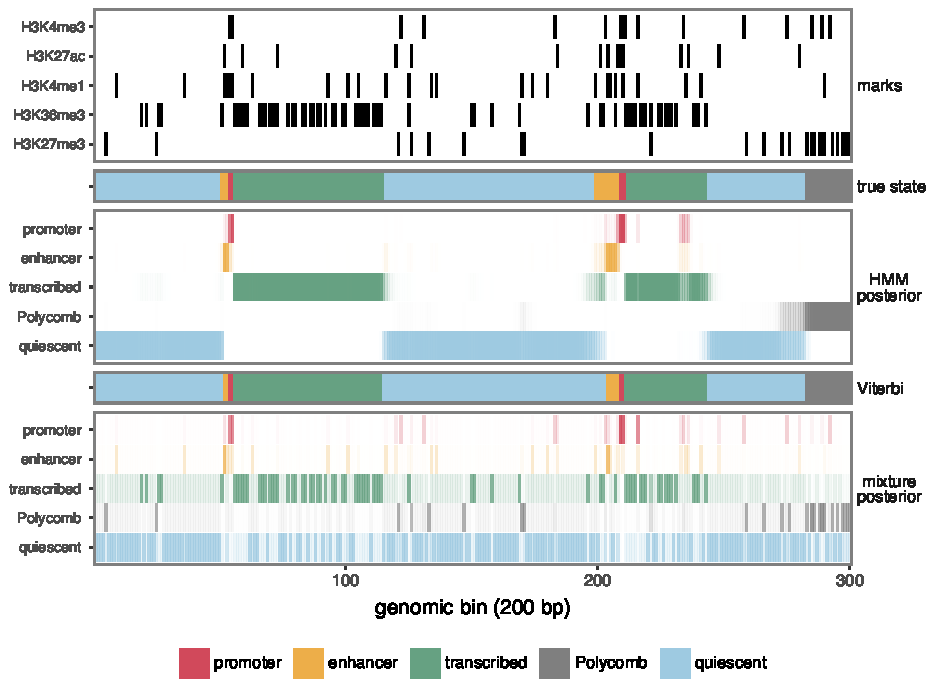
\includegraphics[width=\linewidth]{hmm_posterior.pdf}
  \caption{Inference in a simulated chromatin HMM, for a window of 300 bins. From top: the binary marks (black, present); the true hidden states; the HMM posterior marginals $\gamma_t(i)$ from forward-backward (opacity proportional to probability); the Viterbi path; and the posterior of a mixture model with the same emission parameters but independent bins. The mixture model's assignments flicker between states wherever marks are missing by chance; the HMM's are smooth.}
  \label{fig:hmm_posterior}
\end{figure}

We then fit the model by Baum-Welch from eight random initializations (Figure~\ref{fig:bw_trace}). Each run increases the log likelihood monotonically and converges within a few tens of iterations, but the runs converge to different local optima. Three runs reach the same highest value, $-1.3318$ per bin, slightly above the log likelihood of the true parameters, $-1.3328$, as expected since the maximum likelihood estimate fits the particular sample. The others stall at lower values, for example by merging two true states into one and splitting another. After permuting the state labels to match the truth, the best run recovers every emission probability to within 0.04 and every transition probability to within 0.02 (Figure~\ref{fig:bw_params}).

\begin{figure}[tbp]
  \centering
  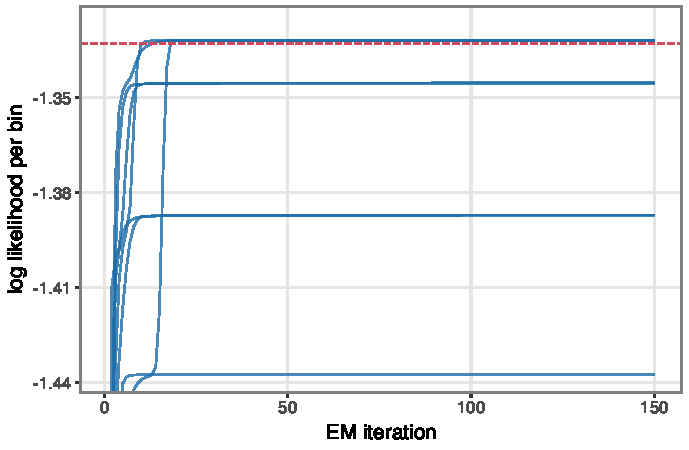
\includegraphics[width=0.7\linewidth]{baum_welch_trace.pdf}
  \caption{Log likelihood per bin during Baum-Welch from eight random initializations on 20{,}000 simulated bins. The dashed line is the log likelihood of the true parameters. Each run increases monotonically, but runs end at different local optima.}
  \label{fig:bw_trace}
\end{figure}

\begin{figure}[tbp]
  \centering
  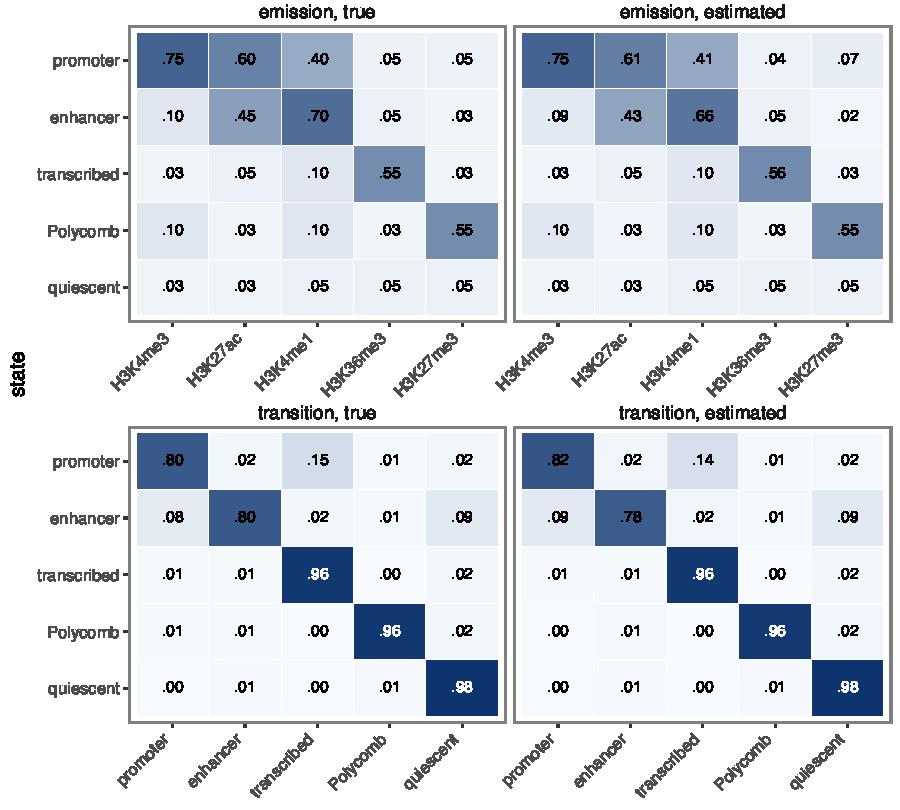
\includegraphics[width=0.85\linewidth]{baum_welch_params.pdf}
  \caption{True (left) and estimated (right) emission matrix $E_{im}=P(y_{tm}=1\mid X_t=i)$ (top) and transition matrix $T_{ij}$ (bottom) for the best of the Baum-Welch runs in Figure~\ref{fig:bw_trace}. Estimated states were relabelled to match the true states.}
  \label{fig:bw_params}
\end{figure}

%======================================================================
\section{ChromHMM in practice}
\label{sec:chromhmm_results}
%======================================================================

\subsection{Chromatin states in nine cell types}

\citet{ernst2011} applied ChromHMM to nine chromatin marks, eight histone modifications and CTCF, measured by ChIP-seq in nine human cell types: embryonic stem cells (H1 ES), the leukaemia cell line K562, the lymphoblastoid cell line GM12878, the liver cancer cell line HepG2, umbilical vein endothelial cells (HUVEC), skeletal muscle myoblasts (HSMM), lung fibroblasts (NHLF), epidermal keratinocytes (NHEK) and mammary epithelial cells (HMEC). Lymphoblastoid cell lines are made by transforming B cells with Epstein-Barr virus, which immortalizes them, and have long been a workhorse of human genetics. The 81 tracks, comprising 2.4 billion reads, were summarized by a single 15-state model learned jointly across all cell types, giving one chromatin state annotation track per cell type.

The states were named after fitting, mainly from their emission parameters (Figure~\ref{fig:chromhmm_emissions}, left). State 1 has high probability of H3K4me3, H3K4me2, H3K27ac and H3K9ac and was labelled an active promoter. States 4 and 5 have strong H3K4me1 with H3K27ac and were labelled strong enhancers; states 6 and 7 have H3K4me1 without H3K27ac and were labelled weak or poised enhancers. State 3 combines H3K4me2 and H3K4me3 with H3K27me3, the bivalent signature of a poised promoter. State 8 is dominated by CTCF and was labelled an insulator. States 9 and 10 carry H3K36me3 and H4K20me1, the marks of transcription, and state 11 a weaker version of the same signal. State 12 carries H3K27me3 alone (Polycomb repression), state 13 has almost no signal (heterochromatin or quiescent), and states 14--15 have high signal for every mark including the input control (WCE), which indicates artefacts from repeats or copy number variation rather than biology. The labels were not given to the model. They are an interpretation, aided by the enrichment of each state in independently annotated genomic features (Figure~\ref{fig:chromhmm_emissions}, right): promoter states are enriched at annotated transcription start sites and CpG islands, transcribed states in gene bodies and at transcription end sites, and the heterochromatin state at the nuclear lamina. Promoters and enhancers both split into several states that differ in signal strength.

\begin{figure}[tbp]
  \centering
  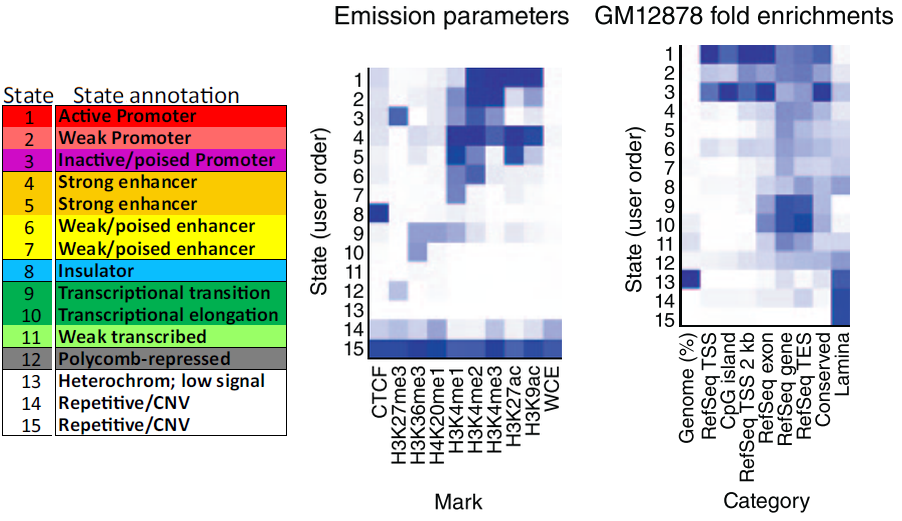
\includegraphics[width=\linewidth]{slides/chromhmm_emissions.png}
  \caption{A 15-state ChromHMM model learned across nine cell types. Left, the state labels assigned after fitting. Middle, emission parameters: the probability of observing each mark in each state (darker is higher). WCE is whole-cell extract, the input control. Right, fold enrichment of each state in genomic annotations in GM12878 cells: transcription start and end sites (TSS, TES), CpG islands, exons, gene bodies, conserved elements and lamina-associated domains; the first column is the percentage of the genome in each state. Reproduced from \citet{ernst2011}.}
  \label{fig:chromhmm_emissions}
\end{figure}

The learned transition matrix (Figure~\ref{fig:chromhmm_transitions}) is close to diagonal. Bins tend to stay in the same state, which is the smoothing effect discussed above. The off-diagonal structure is weak but interpretable: for example, the weak promoter state transitions to the weak enhancer states, and several states transition to the heterochromatin state. A full $K\times K$ matrix is arguably more flexible than needed, since a single self-transition probability per state would capture most of it, but learning it costs little.

\begin{figure}[tbp]
  \centering
  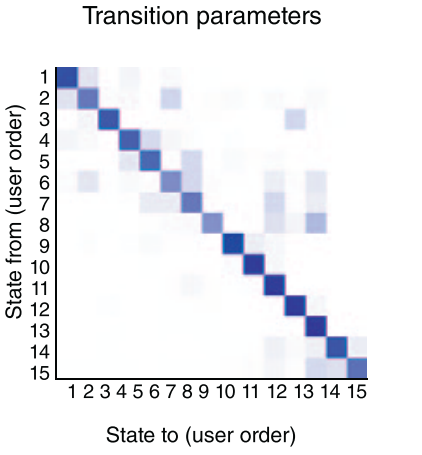
\includegraphics[width=0.5\linewidth]{slides/chromhmm_transitions.png}
  \caption{Transition matrix of the 15-state model in Figure~\ref{fig:chromhmm_emissions}; entry $(i,j)$ is $T_{ij}$, darker is higher. Reproduced from \citet{ernst2011}.}
  \label{fig:chromhmm_transitions}
\end{figure}

\subsection{Cell-type-specific activity}

State definitions are shared across cell types, so the same combinations of marks are found in each, but state locations are cell type specific. Figure~\ref{fig:chromhmm_celltypes} shows a region of chromosome 1 around the gene \textit{WLS}. In the five cell types on the right (HUVEC, HSMM, NHLF, NHEK and HMEC) the gene has an active promoter (red) followed by transcribed states (green) and nearby enhancers (orange, yellow). In K562, GM12878 and HepG2 it is mostly in the quiescent or Polycomb-repressed states and is probably not expressed; the raw data show no H3K27ac there. In H1 ES cells the promoter is in the poised state (purple), with high H3K27me3: the gene is silent but primed for activation during differentiation.

\begin{figure}[tbp]
  \centering
  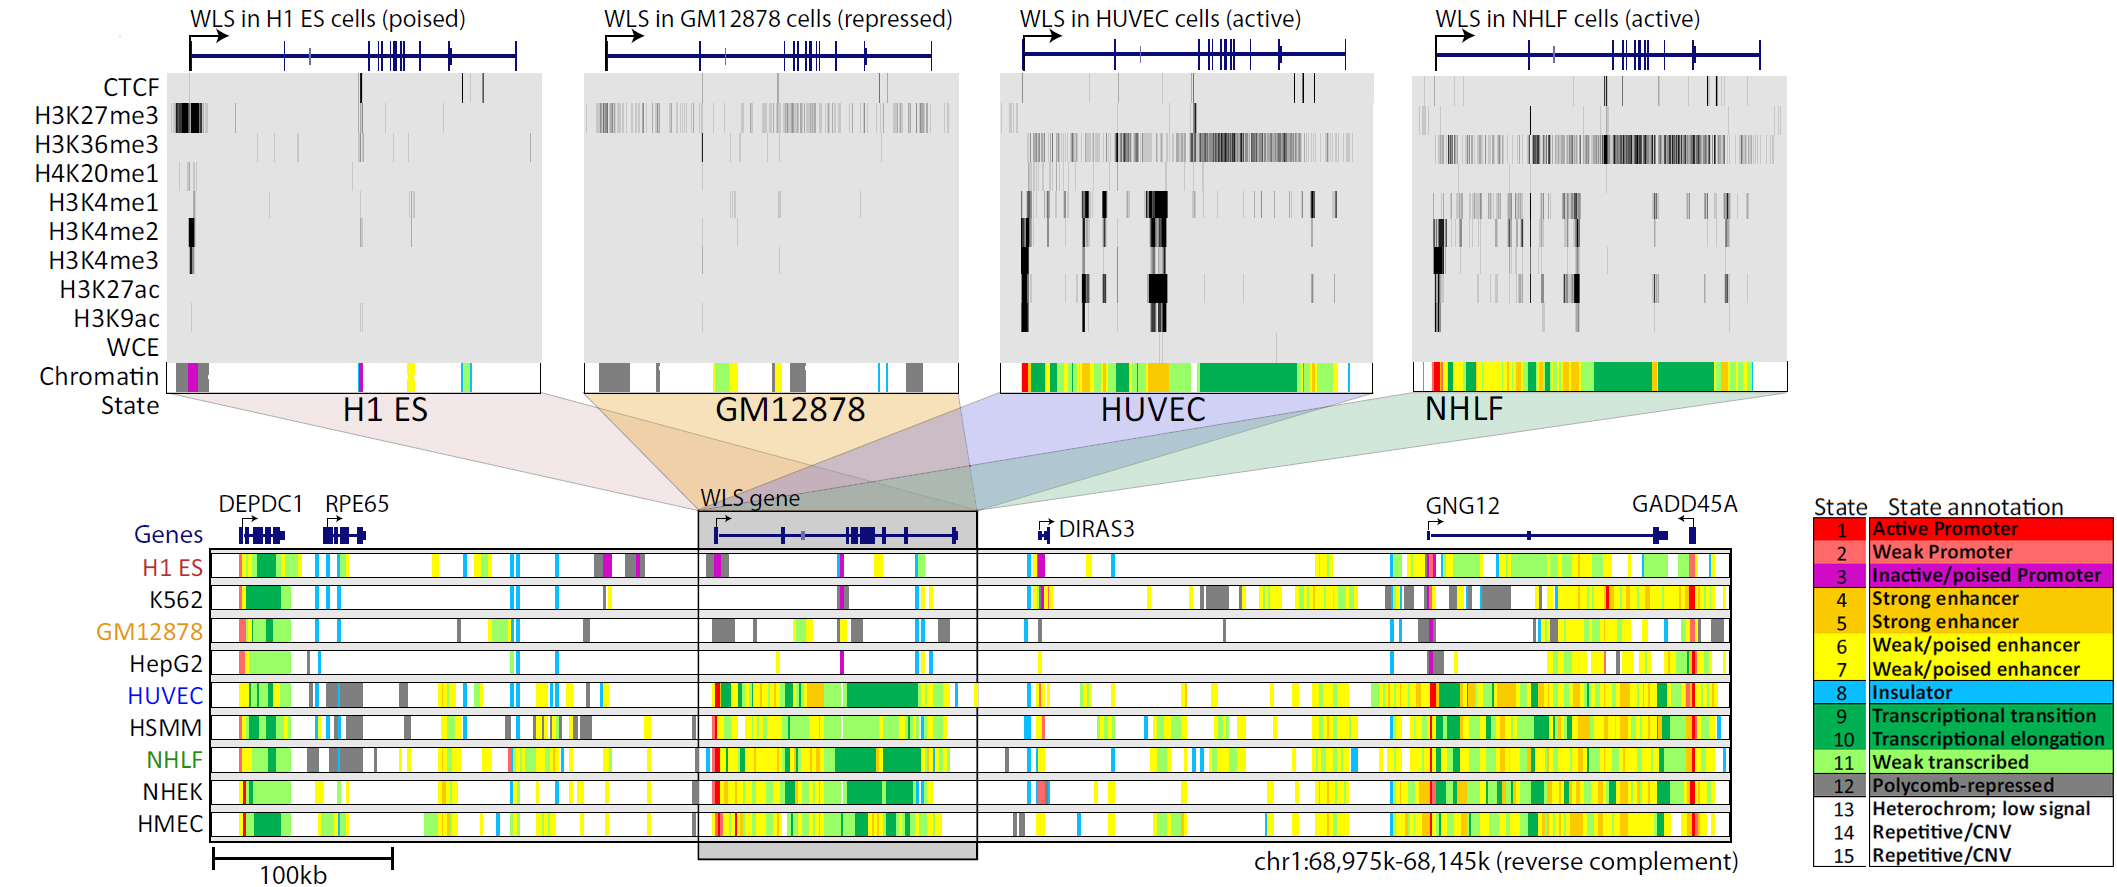
\includegraphics[width=\linewidth]{slides/chromhmm_nine_celltypes.png}
  \caption{Chromatin states across nine cell types in an 830 kb region of chromosome 1 containing the gene \textit{WLS}. Middle, one row of states per cell type, coloured by the legend at right. Top, the underlying binarized ChIP-seq data around \textit{WLS} in four cell types, where it is poised (H1 ES), repressed (GM12878) or active (HUVEC, NHLF). Reproduced from \citet{ernst2011}.}
  \label{fig:chromhmm_celltypes}
\end{figure}

The Roadmap Epigenomics project applied the same approach to 111 reference epigenomes~\citep{roadmap2015}, and the approach has since been applied to hundreds of cell types (Figure~\ref{fig:pax5}). Stacking the annotations of many cell types, each row a cell type and each column a genomic bin, shows which elements are active in which cell types. Promoters of broadly expressed genes are active almost everywhere, while many enhancers are active only in one lineage. Across cell types, roughly 25{,}000 genes and of the order of one to two million candidate regulatory elements have been catalogued~\citep{roadmap2015,encode2020}; the exact number depends on thresholds and is probably an overestimate of truly functional elements.

\begin{figure}[tbp]
  \centering
  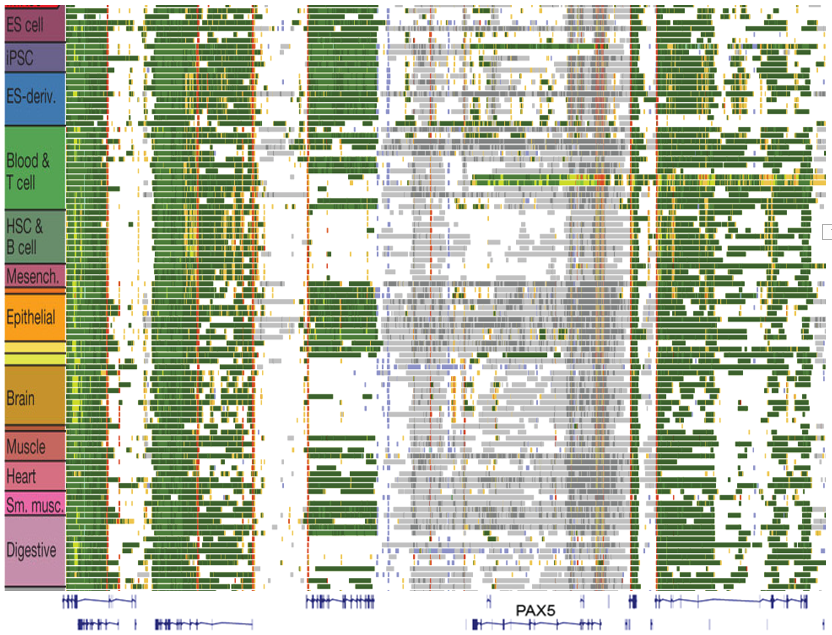
\includegraphics[width=0.85\linewidth]{slides/pax5_states_celltypes.png}
  \caption{Chromatin states around the B cell transcription factor gene \textit{PAX5} (bottom) across many cell and tissue types (rows, grouped by lineage at left). Green indicates transcribed states, red and orange active regulatory states, and grey repressed states. Elements and genes are active in some lineages and repressed in others. \textbf{[Source to be confirmed; likely the Roadmap Epigenomics Consortium~\citep{roadmap2015}.]}}
  \label{fig:pax5}
\end{figure}

\subsection{Uses of chromatin state annotations}

Chromatin state maps are a foundation for much downstream work. A common use is to interpret disease-associated genetic variants (Chapter 11). If variants associated with a disease are enriched in the enhancers of a particular cell type, that cell type is likely relevant to the disease. For Alzheimer's disease, risk variants are most enriched in enhancers active in microglia, the immune cells of the brain, rather than in neurons, astrocytes or oligodendrocytes~\citep{nott2019}, which implicates the immune system in a disease long thought of as neuronal. The annotations also prioritize elements for experimental perturbation.

They also pose machine learning problems that later chapters take up: predicting regulatory elements and their cell-type-specific activity from sequence (Chapters 2 and 3), predicting which elements regulate which genes in which cell types, and predicting gene expression from the activity of regulatory elements.

ChromHMM is still widely used, but it is not the only approach. Segway~\citep{hoffman2012} uses a dynamic Bayesian network with continuous (Gaussian) emissions at single base-pair resolution, and \citet{libbrecht2021} review the broader family of genome segmentation methods.

\subsection{Choosing the number of states}

Choosing $K$ was one of several practical challenges in the original work, along with training on all chromosomes and converting continuous signal into binary calls~\citep{ernst2010}. \citet{ernst2010} learned models with many states and then derived compact models with fewer states that captured the distinctions of the larger ones, a nested approach. The result is a model whose states are interpretable and whose distinctions are supported by the data, but the choice is a judgement call. Other researchers rerunning the analysis with a different $K$ or different initialization would obtain somewhat different states.

%======================================================================
\section{Summary}
%======================================================================

\begin{itemize}
  \item Chromatin states are recurring combinations of histone modifications and other chromatin marks, which correspond to region types such as promoters, enhancers, transcribed regions, insulators and repressed or poised regions. ChromHMM learns them from binarized ChIP-seq data in 200 bp bins.
  \item Directed graphical models represent a joint distribution as a product of conditionals of each variable given its parents. Confounders make variables dependent but conditionally independent; colliders make independent variables dependent once observed (explaining away).
  \item An HMM generalizes a mixture (clustering) model by making the cluster assignments of consecutive positions dependent through a transition matrix $\mT$. The emission parameters $\mE$ play the role of cluster centres.
  \item The forward-backward algorithm computes the posterior marginal of every state, and the likelihood, in $O(SK^2)$ time by passing messages along the chain, instead of summing over $K^{S}$ state sequences. It is the sum-product (belief propagation) algorithm on a chain. The Viterbi algorithm finds the single most probable state sequence.
  \item The Baum-Welch algorithm is EM for the HMM: it alternates between forward-backward (E step) and re-estimating $\vpi$, $\mT$ and $\mE$ from expected counts (M step). The likelihood increases monotonically, but the solution depends on the initialization.
  \item States are named after fitting from their emission parameters and enrichments. Their definitions are shared across cell types while their locations are cell type specific, which reveals cell type identity and helps interpret disease-associated variants.
\end{itemize}

%======================================================================
\section*{Exercises}
%======================================================================

\begin{enumerate}
  \item For the confounder graph of Figure~\ref{fig:dag}b, choose numerical values of $P(C)$, $P(A\mid C)$ and $P(B\mid C)$ and verify that $P(B=1\mid A=1)>P(B=1)$ but $P(B=1\mid A=1,C=1)=P(B=1\mid C=1)$.
  \item Show that if every row of $\mT$ equals $\vpi$, the HMM posterior marginals~\eqref{eq:gamma} reduce to the responsibilities of a mixture model, $\gamma_t(i)\propto\pi_i\phi_t(i)$.
  \item Show that $\sum_{j}\xi_t(i,j)=\gamma_{t-1}(i)$ using~\eqref{eq:gamma} and~\eqref{eq:xi}, and hence that the rows of $\hat\mT$ sum to one.
  \item Derive the update for $E_{im}$ under Bernoulli emissions with a $\text{Beta}(\alpha,\alpha)$ prior on each $E_{im}$, using MAP estimation in the M step. Interpret $\alpha$ as a pseudocount.
  \item Suppose the observations are read counts $y_t\in\{0,1,2,\dots\}$ rather than binary calls, with $y_t\mid X_t=i\sim\text{Poisson}(\lambda_i)$. Which parts of forward-backward and Baum-Welch change? Derive the M-step update for $\lambda_i$.
  \item Implement forward-backward and check it against brute-force enumeration of all $K^S$ state sequences for $K=3$, $S=5$. Then implement Viterbi and confirm that it returns the most probable sequence.
  \item Simulate data from the model of Section~\ref{sec:simulation} and fit it with $K=3$, $5$ and $8$ states. How do the learned emission matrices relate to the true states? What happens to the log likelihood as $K$ increases?
\end{enumerate}

\bibliographystyle{abbrvnat}
\bibliography{../chapter06/chapter06}
\endgroup

% Generated wrapper: chapter 07 with its own figure path, macros and bibliography.
\graphicspath{{../chapter07/figures/}}
\makeatletter\def\input@path{{../chapter07/}}\makeatother
\begingroup
% Chapter 7: recurrent neural networks and DNA methylation.
% Requires: amsmath, amssymb, bm, graphicx, booktabs, subcaption, tikz (arrows.meta, positioning, calc,
% decorations.pathreplacing, fit), natbib.
% Computed figures are produced by scripts/make_figures.py; figures/slides/ holds figures taken from the lecture slides.

\providecommand{\R}{\mathbb{R}}
\providecommand{\E}{\mathbb{E}}
\providecommand{\Normal}{\mathcal{N}}
\providecommand{\argmax}{\operatorname*{arg\,max}}
\providecommand{\argmin}{\operatorname*{arg\,min}}
\providecommand{\vy}{\mathbf{y}}
\providecommand{\vx}{\mathbf{x}}
\providecommand{\mX}{\mathbf{X}}
\providecommand{\mI}{\mathbf{I}}
\providecommand{\vb}{\boldsymbol{\beta}}
\providecommand{\veps}{\boldsymbol{\epsilon}}
\providecommand{\vp}{\mathbf{p}}
\providecommand{\vg}{\mathbf{g}}
\providecommand{\ind}{\mathbf{1}}
% new in this chapter
\providecommand{\vh}{\mathbf{h}}
\providecommand{\va}{\mathbf{a}}
\providecommand{\vc}{\mathbf{c}}
\providecommand{\vz}{\mathbf{z}}
\providecommand{\vr}{\mathbf{r}}
\providecommand{\vi}{\mathbf{i}}
\providecommand{\vo}{\mathbf{o}}
\providecommand{\vf}{\mathbf{f}}
\providecommand{\vu}{\mathbf{u}}
\providecommand{\vbias}{\mathbf{b}}
\providecommand{\vone}{\mathbf{1}}
\providecommand{\vphi}{\boldsymbol{\phi}}
\providecommand{\vpi}{\boldsymbol{\pi}}
\providecommand{\vtheta}{\boldsymbol{\theta}}
\providecommand{\vdelta}{\boldsymbol{\delta}}
\providecommand{\mW}{\mathbf{W}}
\providecommand{\mJ}{\mathbf{J}}
\providecommand{\mT}{\mathbf{T}}
\providecommand{\diag}{\operatorname{diag}}

\chapter{Recurrent neural networks and DNA methylation}
\label{ch:rnn}

Chapter 6 modelled a sequence of genomic bins with a hidden Markov model (HMM): a chain of discrete hidden states, each emitting an observation, with information passed along the chain by the forward-backward algorithm. Recurrent neural networks (RNNs) are the deep learning counterpart. An RNN also carries a hidden state along a sequence, but the state is a continuous vector, it is updated by a learned nonlinear function, and the whole model is trained end to end by gradient descent. This chapter introduces the basic or ``vanilla'' RNN, shows why it is hard to train on long sequences (the exploding and vanishing gradient problem), and describes the gated architectures that fix it, the gated recurrent unit (GRU) and long short-term memory (LSTM). We then cover bidirectional RNNs and the linear RNNs that underlie several recent DNA language models. The application is DNA methylation, a chemical modification of DNA itself, measured by bisulfite sequencing. We describe DeepCpG, a model that combines a convolutional network on DNA sequence with a bidirectional GRU to impute methylation states in single cells.

%======================================================================
\section{Recurrent neural networks}
\label{sec:rnn}
%======================================================================

\subsection{The recurrence}

Consider a sequence of inputs $\vx_1,\dots,\vx_S$ of length $S$, with $\vx_t\in\R^P$. For DNA, $\vx_t$ might be the one-hot encoding of the nucleotide at position $t$ ($P=4$); for the chromatin data of Chapter 6, it might be the vector of $P$ histone marks measured in bin $t$. An RNN maintains a \emph{hidden state} $\vh_t\in\R^K$, starting from an initial state $\vh_0$ (usually $\mathbf{0}$), and updates it one position at a time,
\begin{equation}
  \vh_t = f_{\mW}(\vh_{t-1},\vx_t), \qquad t=1,\dots,S,
  \label{eq:rnn}
\end{equation}
where $f_{\mW}$ is a small neural network with parameters $\mW$ (Figure~\ref{fig:rnn_unrolled}). The hidden states play the same role as the hidden units of the multilayer perceptrons and CNNs of Chapter 2: they are intermediate quantities the network computes, not observed data. Semantically they resemble the latent states of an HMM, a summary of the sequence so far, except that here they are deterministic functions of the input. If we want predictions, a second network $g_{\vtheta}$ maps each hidden state to an output,
\begin{equation}
  \vy_t = g_{\vtheta}(\vh_t),
  \label{eq:rnn_out}
\end{equation}
with $\vy_t\in\R^D$. For example, $g_{\vtheta}$ could be a softmax over $D$ classes, $\vy_t=\operatorname{softmax}(\mW_y\vh_t+\vbias_y)$ with $\mW_y\in\R^{D\times K}$ and $\vbias_y\in\R^D$.

The word \emph{recurrent} refers to the fact that the same function $f_{\mW}$, with the same parameters, is applied at every position. An RNN is in effect a \texttt{for} loop along the sequence. Drawing one copy of $f_{\mW}$ per position, as in Figure~\ref{fig:rnn_unrolled}, is called \emph{unrolling} the network. The unrolled network is an ordinary deep network with $S$ layers that share their weights, and it is trained by backpropagation through this unrolled graph, which is called \emph{backpropagation through time}~\citep{werbos1990}. Weight sharing across positions is the same idea as in a convolutional layer, which applies the same filter at every position. The difference is that a convolution looks at a fixed window of the input, while the RNN hidden state can in principle carry information from arbitrarily far back.

\begin{figure}[t]
  \centering
  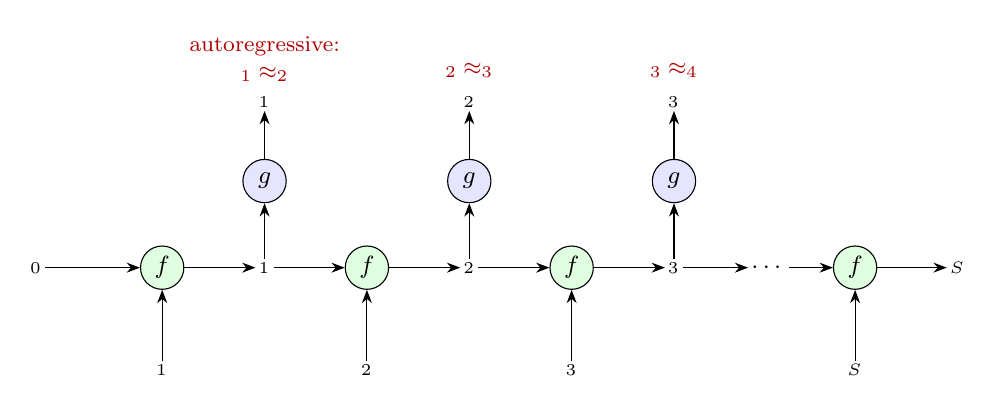
\begin{tikzpicture}[>=Stealth, every node/.style={font=\small},
      f/.style={draw, circle, minimum size=0.55cm, inner sep=0pt, fill=green!12},
      lab/.style={inner sep=1pt}]
    \node[lab] (h0) at (0,0) {$\vh_0$};
    \foreach \i/\x in {1/1.6, 2/4.2, 3/6.8} {
      \node[f] (f\i) at (\x,0) {$f$};
      \node[lab] (x\i) at (\x,-1.3) {$\vx_{\i}$};
      \node[lab] (h\i) at (\x+1.3,0) {$\vh_{\i}$};
      \node[f, fill=blue!10] (g\i) at (\x+1.3,1.1) {$g$};
      \node[lab] (y\i) at (\x+1.3,2.1) {$\vy_{\i}$};
      \draw[->] (x\i) -- (f\i);
      \draw[->] (f\i) -- (h\i);
      \draw[->] (h\i) -- (g\i);
      \draw[->] (g\i) -- (y\i);
    }
    \draw[->] (h0) -- (f1);
    \draw[->] (h1) -- (f2);
    \draw[->] (h2) -- (f3);
    \node[lab] (dots) at (9.3,0) {$\cdots$};
    \draw[->] (h3) -- (dots);
    \node[f] (fS) at (10.4,0) {$f$};
    \node[lab] (xS) at (10.4,-1.3) {$\vx_S$};
    \node[lab] (hS) at (11.7,0) {$\vh_S$};
    \draw[->] (dots) -- (fS); \draw[->] (xS) -- (fS); \draw[->] (fS) -- (hS);
    \node[red!70!black, font=\footnotesize, align=center] at (2.9,2.65) {autoregressive:\\$\vy_1\approx\vx_2$};
    \node[red!70!black, font=\footnotesize] at (5.5,2.5) {$\vy_2\approx\vx_3$};
    \node[red!70!black, font=\footnotesize] at (8.1,2.5) {$\vy_3\approx\vx_4$};
  \end{tikzpicture}
  \caption{An RNN unrolled along a sequence. The same function $f$ (with parameters $\mW$) updates the hidden state from the previous state and the current input; the same function $g$ (with parameters $\vtheta$) maps each hidden state to an output. For autoregressive modelling, the output at position $t$ predicts the input at position $t+1$.}
  \label{fig:rnn_unrolled}
\end{figure}

\subsection{Why recurrent networks?}

Compared with the networks we have seen so far, RNNs have four attractive properties.
\begin{enumerate}
  \item \emph{Flexible input and output lengths.} A CNN followed by dense layers has dimensions that fix the input length. Sequences that are too short must be padded and sequences that are too long trimmed. An RNN runs for as many steps as the sequence has, and it can also generate an output sequence of any length, for example by emitting a stop token when it is done.
  \item \emph{Long-range interactions.} Information in $\vx_1$ can flow through the hidden states to any later position, however long the sequence. A CNN can only relate positions within its receptive field, which grows with depth (Chapter 3). In practice, as we will see, a vanilla RNN finds it hard to retain information over long distances.
  \item \emph{Complex ``grammar''.} Recall from Chapter 2 that regulatory sequences have a grammar: for example, two transcription factors may need to bind near each other, but not too near or too far. Theoretical and empirical work on formal languages suggests that, for a given depth, recurrent networks can represent some sequence rules that CNNs and transformers struggle with. A standard example is parity, deciding whether a binary sequence contains an odd or even number of ones, which an RNN solves by flipping a bit in its state at every one, but which transformers find hard to learn in a way that generalizes to longer sequences~\citep{deletang2023}.
  \item \emph{Causality.} The hidden state $\vh_t$ depends only on $\vx_1,\dots,\vx_t$. This is exactly what is needed for \emph{autoregressive} modelling, predicting the next element from the previous ones, which is the basis of GPT-style language models. We can train the outputs to satisfy $\vy_t\approx\vx_{t+1}$ (Figure~\ref{fig:rnn_unrolled}) without any risk that the model ``cheats'' by seeing $\vx_{t+1}$, because $\vx_{t+1}$ does not influence $\vh_t$. A CNN or transformer needs explicit masking to achieve the same (Chapter 3).
\end{enumerate}

For autoregressive modelling of a DNA sequence, let $\vy_t\in\R^4$ be a softmax over the four nucleotides and $s_{t}\in\{1,\dots,4\}$ the nucleotide at position $t$. The chain rule of probability factorizes the probability of the whole sequence into next-nucleotide predictions,
\begin{equation}
  p(s_1,\dots,s_S) = p(s_1)\prod_{t=2}^{S}p(s_t\mid s_1,\dots,s_{t-1}),
  \qquad p(s_{t+1}=d\mid s_1,\dots,s_t) = y_{td},
\end{equation}
and the negative log likelihood $-\sum_{t=1}^{S-1}\log y_{t,s_{t+1}}$ is a sum of cross-entropy losses, one per position. Because $\vh_t$ summarizes $s_1,\dots,s_t$, the RNN represents the full conditional $p(s_{t+1}\mid s_{1:t})$ rather than the first-order Markov dependence of Chapter 6.

\subsection{Input and output configurations}

The flexibility in sequence length allows several configurations (Figure~\ref{fig:configs}).
\begin{itemize}
  \item \emph{One to one}: no sequence dimension at all. This is an ordinary multilayer perceptron, such as the network of Chapter 2.
  \item \emph{One to many}: generate a sequence from a single input. An example is generating protein sequences, or designing promoter or enhancer sequences that drive expression in a chosen cell type, which is of interest for gene therapy.
  \item \emph{Many to one}: map a sequence to a single output, the setting of the CNNs of Chapters 2 and 3 for predicting transcription factor binding or chromatin accessibility. An RNN allows the input regions to have different lengths, where a CNN forces all peaks to a common width.
  \item \emph{Many to many, different lengths}: encode an input sequence into a hidden state and then decode an output sequence of a different length. The classic example is machine translation~\citep{sutskever2014}, since a sentence need not have the same number of words in two languages.
  \item \emph{Many to many, same length}: one output per input position. Chromatin state annotation, the ChromHMM task of Chapter 6, is an example, as is autoregressive next-token prediction.
\end{itemize}

\begin{figure}[t]
  \centering
  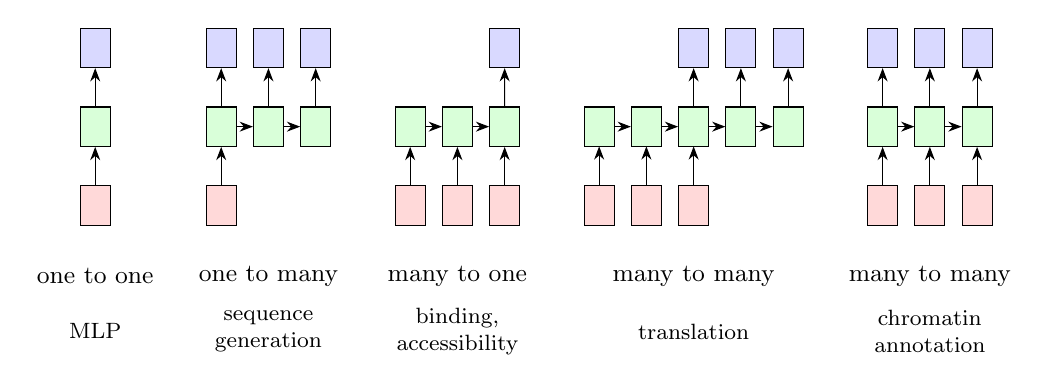
\begin{tikzpicture}[>=Stealth, every node/.style={font=\small},
      inb/.style={draw, fill=red!15, minimum width=0.38cm, minimum height=0.5cm, inner sep=0pt},
      hb/.style={draw, fill=green!15, minimum width=0.38cm, minimum height=0.5cm, inner sep=0pt},
      ob/.style={draw, fill=blue!15, minimum width=0.38cm, minimum height=0.5cm, inner sep=0pt}]
    % one to one
    \begin{scope}[xshift=0cm]
      \node[inb] (i) at (0,0) {}; \node[hb] (h) at (0,1) {}; \node[ob] (o) at (0,2) {};
      \draw[->] (i) -- (h); \draw[->] (h) -- (o);
      \node[align=center] at (0,-0.9) {one to one};
    \end{scope}
    % one to many
    \begin{scope}[xshift=1.6cm]
      \node[inb] (i) at (0,0) {};
      \foreach \k in {0,1,2} { \node[hb] (h\k) at (0.6*\k,1) {}; \node[ob] (o\k) at (0.6*\k,2) {}; \draw[->] (h\k) -- (o\k); }
      \draw[->] (i) -- (h0); \draw[->] (h0) -- (h1); \draw[->] (h1) -- (h2);
      \node[align=center] at (0.6,-0.9) {one to many};
    \end{scope}
    % many to one
    \begin{scope}[xshift=4.0cm]
      \foreach \k in {0,1,2} { \node[inb] (i\k) at (0.6*\k,0) {}; \node[hb] (h\k) at (0.6*\k,1) {}; \draw[->] (i\k) -- (h\k); }
      \node[ob] (o) at (1.2,2) {};
      \draw[->] (h0) -- (h1); \draw[->] (h1) -- (h2); \draw[->] (h2) -- (o);
      \node[align=center] at (0.6,-0.9) {many to one};
    \end{scope}
    % many to many, different lengths
    \begin{scope}[xshift=6.4cm]
      \foreach \k in {0,1,2} { \node[inb] (i\k) at (0.6*\k,0) {}; \draw[->] (i\k) -- ++(0,0.75); }
      \foreach \k in {0,...,4} { \node[hb] (h\k) at (0.6*\k,1) {}; }
      \foreach \k in {2,3,4} { \node[ob] (o\k) at (0.6*\k,2) {}; \draw[->] (h\k) -- (o\k); }
      \foreach \k/\j in {0/1,1/2,2/3,3/4} \draw[->] (h\k) -- (h\j);
      \node[align=center] at (1.2,-0.9) {many to many};
    \end{scope}
    % many to many, same length
    \begin{scope}[xshift=10.0cm]
      \foreach \k in {0,1,2} { \node[inb] (i\k) at (0.6*\k,0) {}; \node[hb] (h\k) at (0.6*\k,1) {}; \node[ob] (o\k) at (0.6*\k,2) {};
        \draw[->] (i\k) -- (h\k); \draw[->] (h\k) -- (o\k); }
      \draw[->] (h0) -- (h1); \draw[->] (h1) -- (h2);
      \node[align=center] at (0.6,-0.9) {many to many};
    \end{scope}
    \node[font=\footnotesize, align=center] at (0,-1.6) {MLP};
    \node[font=\footnotesize, align=center] at (2.2,-1.6) {sequence\\generation};
    \node[font=\footnotesize, align=center] at (4.6,-1.6) {binding,\\accessibility};
    \node[font=\footnotesize, align=center] at (7.6,-1.6) {translation};
    \node[font=\footnotesize, align=center] at (10.6,-1.6) {chromatin\\annotation};
  \end{tikzpicture}
  \caption{Input and output configurations of RNNs. Red boxes are inputs, green boxes hidden states and blue boxes outputs; horizontal arrows are the recurrence. Below each configuration is an example application. After \citet{karpathy2015}.}
  \label{fig:configs}
\end{figure}

%======================================================================
\section{The vanilla RNN}
\label{sec:vanilla}
%======================================================================

The simplest choice of $f_{\mW}$ in~\eqref{eq:rnn}, sometimes called the Elman network~\citep{elman1990}, is a single dense layer applied to the previous hidden state and the current input,
\begin{equation}
  \vh_t = \tanh\left(\mW_h\vh_{t-1} + \mW_x\vx_t + \vbias\right),
  \label{eq:vanilla}
\end{equation}
where $\mW_h\in\R^{K\times K}$, $\mW_x\in\R^{K\times P}$ and $\vbias\in\R^K$, and $\tanh$ acts elementwise. Stacking the previous state and the input into one vector of length $K+P$ and the two weight matrices side by side, $\mW=[\mW_h\ \mW_x]\in\R^{K\times(K+P)}$, gives the equivalent form
\begin{equation}
  \vh_t = \tanh\left(\mW\begin{bmatrix}\vh_{t-1}\\\vx_t\end{bmatrix} + \vbias\right).
\end{equation}
So the vanilla RNN concatenates its two inputs, applies a linear map and a nonlinearity. It has $K(K+P+1)$ parameters regardless of the sequence length.

The hyperbolic tangent, $\tanh(a)=(e^a-e^{-a})/(e^a+e^{-a})$, is the usual activation for recurrences (Figure~\ref{fig:tanh}). It is a rescaled logistic sigmoid, $\tanh(a)=2\sigma(2a)-1$, so it saturates at $\pm1$ rather than at 0 and 1. Its range is symmetric about zero, which suits a hidden state that is fed back into the next step, and bounding the state stops it from growing without limit along the sequence. Its derivative is
\begin{equation}
  \tanh'(a) = 1-\tanh(a)^2,
  \label{eq:tanh_deriv}
\end{equation}
a bump with maximum $\tanh'(0)=1$ that decays to zero as $|a|$ grows. The derivative of the sigmoid has the same shape but a maximum of only $1/4$.

\begin{figure}[t]
  \centering
  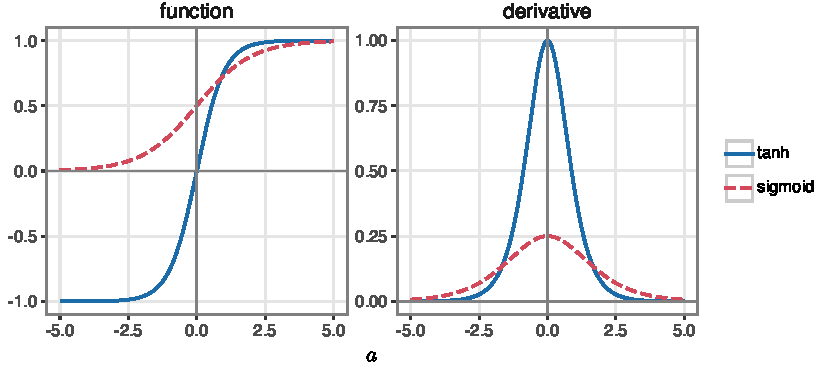
\includegraphics[width=0.85\linewidth]{tanh.pdf}
  \caption{The $\tanh$ and logistic sigmoid functions (left) and their derivatives (right). The derivative of $\tanh$ is at most 1, attained at $a=0$, and decays to zero when the unit saturates.}
  \label{fig:tanh}
\end{figure}

%======================================================================
\section{Exploding and vanishing gradients}
\label{sec:gradients-07}
%======================================================================

\subsection{Backpropagation through time}

To train an RNN we need the gradient of the loss with respect to the shared weights. Suppose the loss is a sum over positions, $L=\sum_{t=1}^S\ell_t(\vy_t)$, for example the next-nucleotide cross-entropy above. Write the vanilla RNN~\eqref{eq:vanilla} in two steps, a pre-activation $\va_t=\mW_h\vh_{t-1}+\mW_x\vx_t+\vbias\in\R^K$ and $\vh_t=\tanh(\va_t)$. The \emph{Jacobian} of one step, the $K\times K$ matrix of partial derivatives $(\mJ_t)_{kj}=\partial h_{tk}/\partial h_{t-1,j}$, is
\begin{equation}
  \mJ_t = \frac{\partial\vh_t}{\partial\vh_{t-1}} = \diag\left(\vone-\vh_t\odot\vh_t\right)\mW_h ,
  \label{eq:vanilla_jac}
\end{equation}
by~\eqref{eq:tanh_deriv} and the chain rule, where $\diag(\cdot)$ makes a diagonal matrix from a vector and $\odot$ is the elementwise product. Here we use the convention that a Jacobian has one row per output and one column per input, so that gradients, written as column vectors, are passed backward by the transposed Jacobian. This is the transpose of the gradient matrix of Chapter 2.

Let $\vdelta_t=\nabla_{\vh_t}L\in\R^K$ be the gradient of the total loss with respect to the hidden state at position $t$. The state $\vh_t$ affects the loss directly, through $\ell_t$, and indirectly, through $\vh_{t+1}$ and therefore all later positions. The multivariate chain rule gives the backward recursion
\begin{equation}
  \vdelta_t = \nabla_{\vh_t}\ell_t + \mJ_{t+1}^\top\vdelta_{t+1}, \qquad \vdelta_S=\nabla_{\vh_S}\ell_S ,
  \label{eq:bptt}
\end{equation}
which runs from $t=S$ down to $t=1$, the RNN analogue of the backward pass of Chapter 2. Unrolling it, the contribution of the loss at a later position $S$ to the gradient at position $t$ is
\begin{equation}
  \nabla_{\vh_t}\ell_S = \left(\frac{\partial\vh_S}{\partial\vh_t}\right)^\top\nabla_{\vh_S}\ell_S,
  \qquad
  \frac{\partial\vh_S}{\partial\vh_t} = \mJ_S\mJ_{S-1}\cdots\mJ_{t+1} = \prod_{r=t+1}^{S}\diag\left(\vone-\vh_r\odot\vh_r\right)\mW_h ,
  \label{eq:jac_product}
\end{equation}
a product of $S-t$ Jacobians, with later positions on the left. Finally, since $\mW_h$ enters every step, its gradient sums over positions,
\begin{equation}
  \nabla_{\mW_h}L = \sum_{t=1}^{S}\left(\vdelta_t\odot(\vone-\vh_t\odot\vh_t)\right)\vh_{t-1}^\top \in\R^{K\times K},
\end{equation}
and similarly for $\mW_x$ (with $\vx_t^\top$ in place of $\vh_{t-1}^\top$) and $\vbias$. Each term is the outer product of the error signal arriving at the pre-activation $\va_t$ and the input to that step, as in Chapter 2. Whether the model can learn that $\vx_t$ matters for a loss many positions later depends on the product~\eqref{eq:jac_product}.

\subsection{The scalar case}

The problem is clearest with a scalar hidden state, $K=1$, where $\mW_h=w$ is a number. Then~\eqref{eq:jac_product} becomes
\begin{equation}
  \frac{\partial h_S}{\partial h_t} = w^{S-t}\prod_{r=t+1}^{S}\tanh'(a_r) .
\end{equation}
Each factor $\tanh'(a_r)$ is at most 1, and close to 1 only when the unit is far from saturation. The factor $w^{S-t}$ goes to zero exponentially fast if $|w|<1$ and blows up exponentially if $|w|>1$. For a sequence of length 100 or 1000 this means the gradient from distant positions either vanishes, so the model cannot learn long-range dependencies, or explodes, so that gradient descent takes enormous, unstable steps. Only $|w|=1$ avoids both, and even then the $\tanh'$ factors shrink the product whenever the unit is not near zero.

\subsection{The matrix case}

For $K>1$ the role of $|w|$ is played by the singular values of $\mW_h$. Let $\|\cdot\|$ be the spectral norm, the largest singular value $\sigma_{\max}(\cdot)$. Since the norm of a product is at most the product of norms and $\|\diag(\vone-\vh_r\odot\vh_r)\|\leq1$,
\begin{equation}
  \left\|\frac{\partial\vh_S}{\partial\vh_t}\right\| \leq \prod_{r=t+1}^S\left\|\diag(\vone-\vh_r\odot\vh_r)\right\|\,\|\mW_h\| \leq \sigma_{\max}(\mW_h)^{S-t}.
\end{equation}
If $\sigma_{\max}(\mW_h)<1$ the gradient is guaranteed to vanish exponentially with distance. If $\sigma_{\max}(\mW_h)>1$ the bound allows growth, and for large enough singular values the gradient does explode~\citep{bengio1994,pascanu2013}. Figure~\ref{fig:gradient_flow} (left) shows this numerically for a vanilla RNN with $K=50$ hidden units, random inputs and a weight matrix $\mW_h$ whose singular values all equal a common value. With singular values of 0.9 the gradient shrinks by more than 20 orders of magnitude over 100 steps; with 1.5 it still shrinks, because saturated units have small $\tanh'$; with 3 it grows by more than 10 orders of magnitude.

The underlying cause is that backpropagation multiplies by the same matrix $\mW_h$ at every step. Forcing $\mW_h$ to have all singular values equal to 1 (an orthogonal matrix) removes the exponential factor but constrains the model heavily, and the $\tanh'$ factors still shrink the gradient. Exploding gradients have a simple practical remedy, \emph{gradient clipping}, which rescales the gradient $\vg$ to $c\,\vg/\|\vg\|$ whenever its norm exceeds a threshold $c$~\citep{pascanu2013}. Vanishing gradients need a change of architecture, which is the subject of the next section.

\begin{figure}[t]
  \centering
  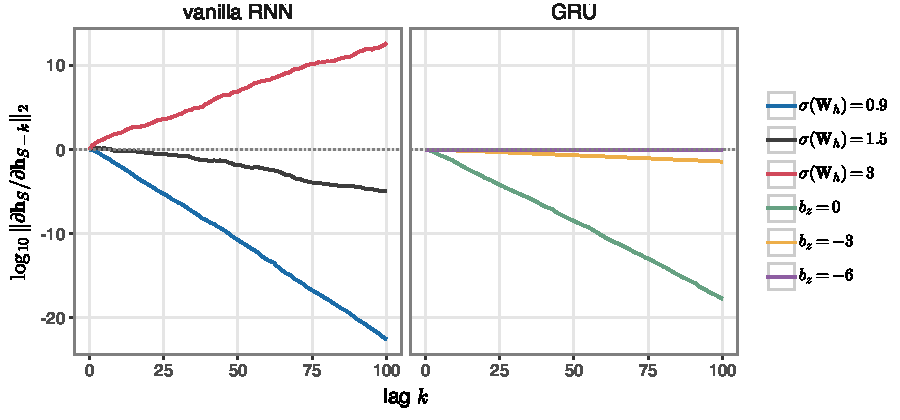
\includegraphics[width=0.95\linewidth]{gradient_flow.pdf}
  \caption{Norm of the Jacobian $\partial\vh_S/\partial\vh_{S-k}$, which scales the gradient that the loss at position $S$ sends back to position $S-k$, for simulated networks with $K=50$ hidden units and random inputs. Left, vanilla RNN with all singular values of $\mW_h$ equal to $\sigma(\mW_h)$: the gradient vanishes exponentially for $\sigma=0.9$, decays more slowly for $\sigma=1.5$, where saturation of $\tanh$ offsets the growth, and explodes for $\sigma=3$. Right, GRU with update-gate bias $b_z$: when the gate is mostly closed ($b_z=-3$ or $-6$, so $z\approx0.05$ or $0.002$) the gradient is preserved over 100 steps.}
  \label{fig:gradient_flow}
\end{figure}

%======================================================================
\section{Gated recurrent networks}
\label{sec:gated}
%======================================================================

The vanilla RNN fails because the backward pass multiplies by the same matrix at every step. Gated architectures fix this by making the step-to-step dependence \emph{data-adaptive}: a learned gate, computed from the current input and state, decides at each position how much of the old state to keep and how much new information to write. Where the gate keeps the old state, the state, and its gradient, pass through nearly unchanged. Historically the long short-term memory (LSTM)~\citep{hochreiter1997} came first and the gated recurrent unit (GRU)~\citep{cho2014} later, as a simplification that performs about as well in practice~\citep{chung2014,jozefowicz2015}. We present the GRU first because it is simpler.

\subsection{Gates}

A \emph{gate} is a vector of numbers between 0 and 1, computed by a logistic sigmoid $\sigma(a)=1/(1+e^{-a})$ applied to a linear function of the current input and the previous state. Let
\begin{equation}
  \vphi_t = \begin{bmatrix}\vx_t\\\vh_{t-1}\end{bmatrix}\in\R^{P+K}
\end{equation}
be their concatenation. Every gate below has the form $\sigma(\mW_\bullet\vphi_t+\vbias_\bullet)\in(0,1)^K$, with its own weights $\mW_\bullet\in\R^{K\times(P+K)}$ and bias $\vbias_\bullet\in\R^K$. A gate is applied by elementwise multiplication, so each of the $K$ hidden units has its own gate value at each position. A gate value near 0 blocks a signal and a value near 1 lets it through.

\subsection{The gated recurrent unit}

The GRU computes two gates and a candidate state,
\begin{align}
  \vz_t &= \sigma\left(\mW_z\vphi_t+\vbias_z\right) && \text{(update gate)},\\
  \vr_t &= \sigma\left(\mW_r\vphi_t+\vbias_r\right) && \text{(reset gate)},\\
  \vg_t &= \tanh\left(\mW_x\vx_t + \vr_t\odot(\mW_h\vh_{t-1}) + \vbias_g\right) && \text{(candidate state)},
\end{align}
with $\mW_x\in\R^{K\times P}$ and $\mW_h\in\R^{K\times K}$ as in the vanilla RNN, and then sets the new state to an elementwise convex combination of the candidate and the old state,
\begin{equation}
  \vh_t = \vz_t\odot\vg_t + (\vone-\vz_t)\odot\vh_{t-1} .
  \label{eq:gru}
\end{equation}
Figure~\ref{fig:gru} shows the computation. The update gate $\vz_t$ acts as a forgetting factor. Where $z_{tk}\approx1$, unit $k$ discards its old value and takes in new information from $\vg_t$; where $z_{tk}\approx0$, it ignores the input and copies its previous value. The candidate $\vg_t$ is a vanilla RNN step~\eqref{eq:vanilla}, except that the reset gate $\vr_t$ controls how much of the previous state is used when processing the new input. In this sense gating resembles attention (Chapter 3): the model learns, from the data, which information to take into account at each position.

\begin{figure}[t]
  \centering
  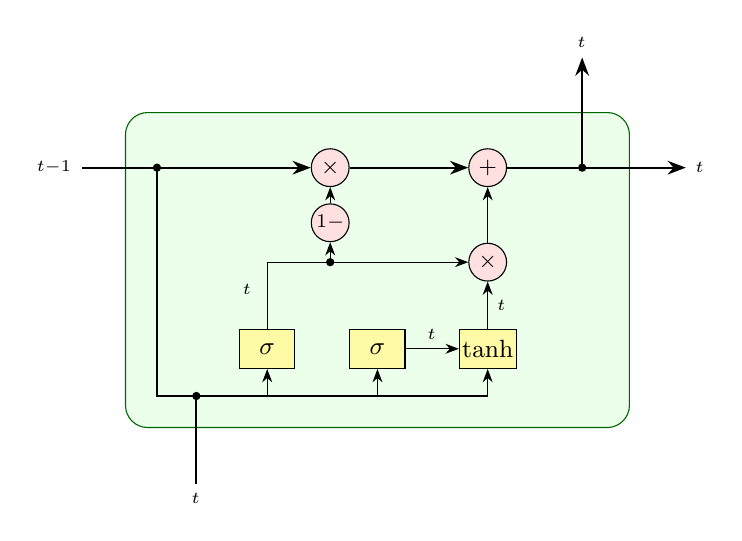
\begin{tikzpicture}[>=Stealth, every node/.style={font=\small},
      gate/.style={draw, fill=yellow!35, minimum width=0.7cm, minimum height=0.5cm, inner sep=1pt},
      op/.style={draw, circle, fill=red!12, minimum size=0.48cm, inner sep=0pt, font=\footnotesize}]
    \draw[rounded corners=8pt, fill=green!8, draw=green!40!black] (0,0) rectangle (6.4,4.0);
    % state line
    \node (hin) at (-0.9,3.3) {$\vh_{t-1}$};
    \node[op] (m1) at (2.6,3.3) {$\times$};
    \node[op] (add) at (4.6,3.3) {$+$};
    \node (hout) at (7.3,3.3) {$\vh_t$};
    \draw[->, thick] (hin) -- (m1); \draw[->, thick] (m1) -- (add); \draw[->, thick] (add) -- (hout);
    \draw[->, thick] (5.8,3.3) -- (5.8,4.7) node[above] {$\vh_t$};
    % input line
    \node (x) at (0.9,-0.9) {$\vx_t$};
    \draw[thick] (0.4,3.3) -- (0.4,0.4) -- (4.6,0.4);
    \draw[thick] (x) -- (0.9,0.4);
    \node[gate] (sz) at (1.8,1.0) {$\sigma$};
    \node[gate] (sr) at (3.2,1.0) {$\sigma$};
    \node[gate] (tg) at (4.6,1.0) {tanh};
    \foreach \g/\xx in {sz/1.8, sr/3.2, tg/4.6} \draw[->] (\xx,0.4) -- (\g);
    % reset gate into candidate
    \draw[->] (sr) -- node[above, font=\footnotesize] {$\vr_t$} (tg);
    % update gate
    \node[op] (m2) at (4.6,2.1) {$\times$};
    \node[op] (oneminus) at (2.6,2.6) {\scriptsize $1-$};
    \draw[->] (sz) -- (1.8,2.1) -- (m2);
    \node[font=\footnotesize] at (1.55,1.75) {$\vz_t$};
    \draw[->] (2.6,2.1) -- (oneminus); \draw[->] (oneminus) -- (m1);
    \draw[->] (tg) -- node[right, font=\footnotesize] {$\vg_t$} (m2);
    \draw[->] (m2) -- (add);
    \fill (0.4,3.3) circle (1.5pt); \fill (0.9,0.4) circle (1.5pt); \fill (2.6,2.1) circle (1.5pt); \fill (5.8,3.3) circle (1.5pt);
  \end{tikzpicture}
  \caption{The gated recurrent unit. Yellow boxes are learned layers, each taking the concatenation of $\vx_t$ and $\vh_{t-1}$; red circles are elementwise operations. The update gate $\vz_t$ mixes the candidate $\vg_t$ with the previous state; the reset gate $\vr_t$ scales the contribution of the previous state to the candidate. Redrawn after \citet{olah2015}.}
  \label{fig:gru}
\end{figure}

Two variants of the candidate are in use. The original GRU~\citep{cho2014} applies the reset gate before the matrix multiplication, $\vg_t=\tanh(\mW_x\vx_t+\mW_h(\vr_t\odot\vh_{t-1})+\vbias_g)$, while the form above, with the gate applied after the multiplication, is the one implemented in common GPU libraries such as cuDNN and PyTorch. Conventions also differ on whether $\vz_t$ or $\vone-\vz_t$ multiplies the old state. None of these choices changes the idea. The reset gate is arguably the least essential component: simplified gated units that drop it perform comparably on many tasks~\citep{feng2024}, a point we return to in Section~\ref{sec:linear}.

\subsection{Why gating fixes the gradient}

Differentiate~\eqref{eq:gru} with respect to $\vh_{t-1}$. The state enters directly, through $(\vone-\vz_t)\odot\vh_{t-1}$, and indirectly, through $\vz_t$ and $\vg_t$. Write $\mW_{z,h}\in\R^{K\times K}$ for the block of $\mW_z$ that multiplies $\vh_{t-1}$, and similarly $\mW_{r,h}$, and $\vu_t=\mW_h\vh_{t-1}$. By the product rule,
\begin{equation}
  \mJ_t = \frac{\partial\vh_t}{\partial\vh_{t-1}}
  = \underbrace{\diag(\vone-\vz_t)}_{\text{direct path}}
  + \diag(\vg_t-\vh_{t-1})\frac{\partial\vz_t}{\partial\vh_{t-1}}
  + \diag(\vz_t)\frac{\partial\vg_t}{\partial\vh_{t-1}},
  \label{eq:gru_jac}
\end{equation}
where
\begin{align}
  \frac{\partial\vz_t}{\partial\vh_{t-1}} &= \diag\left(\vz_t\odot(\vone-\vz_t)\right)\mW_{z,h},\\
  \frac{\partial\vg_t}{\partial\vh_{t-1}} &= \diag\left(\vone-\vg_t\odot\vg_t\right)\left[\diag(\vr_t)\mW_h + \diag(\vu_t)\diag\left(\vr_t\odot(\vone-\vr_t)\right)\mW_{r,h}\right],
\end{align}
using $\sigma'(a)=\sigma(a)(1-\sigma(a))$. Consider a unit whose update gate is nearly closed, $z_{tk}\approx0$. Then both $z_{tk}(1-z_{tk})$ and $z_{tk}$ are close to zero, so the second and third terms of row $k$ of~\eqref{eq:gru_jac} vanish, and the row is close to the corresponding row of the identity. The direct path contributes
\begin{equation}
  (\vone-\vz_t)\odot\nabla_{\vh_t}L
\end{equation}
to the gradient $\nabla_{\vh_{t-1}}L$. This is an elementwise product with a gate that differs at every position, not a repeated multiplication by the same matrix. Over many positions the product of the factors $1-z_{tk}$ stays close to 1 for as long as the unit keeps its memory, so neither vanishing nor explosion occurs along this path. Where the unit does take in new input, the gradient is deliberately cut, since the old state no longer matters.

Figure~\ref{fig:gradient_flow} (right) illustrates this with a GRU of the same size, with random weights and the bias of the update gate set to $b_z$ for all units. With $b_z=0$ the gates are around $1/2$, each step roughly halves the direct path, and the gradient vanishes much as in the vanilla RNN. With $b_z=-3$ or $-6$ the gates are mostly closed and the gradient is preserved over 100 positions. A trained GRU learns gate values that are small where information must be carried and large where it should be overwritten.

\subsection{Long short-term memory}

The LSTM~\citep{hochreiter1997,gers2000} separates two roles that the GRU state plays. Besides the hidden state $\vh_t\in\R^K$, which is the output at each position and acts as short-term memory, it carries a \emph{cell state} $\vc_t\in\R^K$ intended as long-term memory (the name has nothing to do with biological cells). With $\vphi_t$ again the concatenation of $\vx_t$ and $\vh_{t-1}$, the LSTM computes three gates and a candidate,
\begin{align}
  \vi_t &= \sigma\left(\mW_i\vphi_t+\vbias_i\right) && \text{(input gate)},\\
  \vf_t &= \sigma\left(\mW_f\vphi_t+\vbias_f\right) && \text{(forget gate)},\\
  \vo_t &= \sigma\left(\mW_o\vphi_t+\vbias_o\right) && \text{(output gate)},\\
  \vg_t &= \tanh\left(\mW_g\vphi_t+\vbias_g\right) && \text{(candidate)},
\end{align}
and updates the two states as
\begin{equation}
  \vc_t = \vf_t\odot\vc_{t-1} + \vi_t\odot\vg_t, \qquad \vh_t = \vo_t\odot\tanh(\vc_t).
  \label{eq:lstm}
\end{equation}
Figure~\ref{fig:lstm} shows the computation. The forget gate decides how much of the old cell state to keep, the input gate how much of the candidate to write, and the output gate how much of the cell state to expose as $\vh_t$. Note that the forget gate of the LSTM is a ``keep'' gate, $f_{tk}\approx1$ retaining the memory, the opposite convention to the GRU's $\vz_t$.

\begin{figure}[t]
  \centering
  \begin{tikzpicture}[>=Stealth, every node/.style={font=\small},
      gate/.style={draw, fill=yellow!35, minimum width=0.7cm, minimum height=0.5cm, inner sep=1pt},
      op/.style={draw, circle, fill=red!12, minimum size=0.48cm, inner sep=0pt, font=\footnotesize}]
    \draw[rounded corners=8pt, fill=green!8, draw=green!40!black] (0,0) rectangle (7.2,4.0);
    % cell line
    \node (cin) at (-0.9,3.3) {$\vc_{t-1}$};
    \node[op] (mf) at (1.5,3.3) {$\times$};
    \node[op] (add) at (3.35,3.3) {$+$};
    \node (cout) at (8.1,3.3) {$\vc_t$};
    \draw[->, thick] (cin) -- (mf); \draw[->, thick] (mf) -- (add); \draw[->, thick] (add) -- (cout);
    % hidden/input line
    \node (hin) at (-0.9,0.4) {$\vh_{t-1}$};
    \node (x) at (0.6,-0.9) {$\vx_t$};
    \draw[thick] (hin) -- (5.2,0.4);
    \draw[thick] (x) -- (0.6,0.4);
    \node[gate] (sf) at (1.5,1.0) {$\sigma$};
    \node[gate] (si) at (2.8,1.0) {$\sigma$};
    \node[gate] (tg) at (3.9,1.0) {tanh};
    \node[gate] (so) at (5.2,1.0) {$\sigma$};
    \foreach \g/\xx in {sf/1.5, si/2.8, tg/3.9, so/5.2} \draw[->] (\xx,0.4) -- (\g);
    \draw[->] (sf) -- node[left, font=\footnotesize] {$\vf_t$} (mf);
    \node[op] (mi) at (3.35,2.2) {$\times$};
    \draw[->] (si) -- (2.8,2.2) node[left, font=\footnotesize] {$\vi_t$} -- (mi);
    \draw[->] (tg) -- (3.9,2.2) node[right, font=\footnotesize] {$\vg_t$} -- (mi);
    \draw[->] (mi) -- (add);
    % output
    \node[op, minimum size=0.6cm] (tc) at (6.2,2.55) {\scriptsize tanh};
    \node[op] (mo) at (6.2,1.6) {$\times$};
    \draw[->] (6.2,3.3) -- (tc); \draw[->] (tc) -- (mo);
    \draw[->] (so) -- (5.2,1.6) node[above, font=\footnotesize] {$\vo_t$} -- (mo);
    \draw[thick] (mo) -- (6.2,0.4);
    \node (hout) at (8.1,0.4) {$\vh_t$};
    \draw[->, thick] (6.2,0.4) -- (hout);
    \draw[->, thick] (6.75,0.4) -- (6.75,4.7) node[above] {$\vh_t$};
    \fill (0.6,0.4) circle (1.5pt); \fill (6.2,3.3) circle (1.5pt); \fill (6.75,0.4) circle (1.5pt);
  \end{tikzpicture}
  \caption{Long short-term memory. The cell state $\vc_t$ (top line) is modified only by elementwise multiplication with the forget gate and addition of the gated candidate; the hidden state $\vh_t$ (bottom line) is a gated, squashed copy of the cell state. Redrawn after \citet{olah2015}.}
  \label{fig:lstm}
\end{figure}

The gradient along the cell state is governed by the same mechanism as in the GRU. Holding the gates fixed, $\partial\vc_t/\partial\vc_{t-1}=\diag(\vf_t)$, so the gradient passed back along the cell line is multiplied elementwise by forget gates that vary with position. In the original LSTM there was no forget gate, equivalent to $\vf_t=\vone$, so that this Jacobian was exactly the identity, an error signal that is carried unchanged; the forget gate was added later so that the network could also learn to reset its memory~\citep{gers2000}. A common practical recommendation is to initialize $\vbias_f$ to a positive value, such as 1, so that the cell remembers by default early in training~\citep{jozefowicz2015}. The hidden state $\vh_t$ depends on $\vh_{t-1}$ only through the gates and the candidate, which feed the cell state, so long-range information travels along the cell line.

\subsection{GRU or LSTM?}

The GRU can be seen as an LSTM with two simplifications. It ties the input and forget gates, setting $\vi_t=\vz_t$ and $\vf_t=\vone-\vz_t$, so that remembering more means writing less and vice versa, and it merges the cell and hidden states. Table~\ref{tab:rnn_params} compares the parameter counts. In large empirical comparisons the two perform similarly, with the best choice depending on the task~\citep{chung2014,jozefowicz2015}. The details of these architectures can feel arbitrary, and the important idea is the gate, a learned, data-dependent control of information flow. The same idea appears elsewhere, for example in gated convolutional networks, where the output of a convolution is multiplied elementwise by a sigmoid gate computed by a second convolution~\citep{dauphin2017}.

\begin{table}[t]
  \centering
  \caption{Recurrent units with input dimension $P$ and hidden dimension $K$. Each learned layer has a $K\times(K+P)$ weight matrix and a bias of length $K$.}
  \label{tab:rnn_params}
  \begin{tabular}{llll}
    \toprule
    Unit & State & Learned layers & Parameters \\
    \midrule
    Vanilla RNN & $\vh_t$ & 1 ($\tanh$) & $K(K+P+1)$ \\
    GRU & $\vh_t$ & 3 (2 gates, candidate) & $3K(K+P+1)$ \\
    LSTM & $\vh_t$, $\vc_t$ & 4 (3 gates, candidate) & $4K(K+P+1)$ \\
    \bottomrule
  \end{tabular}
\end{table}

%======================================================================
\section{Bidirectional and deep RNNs}
\label{sec:bidir}
%======================================================================

Causality is an advantage for autoregressive modelling but a limitation when we want the prediction at a position to use the sequence on both sides of it, as for chromatin annotation, where the state of a bin depends on its neighbours in both directions. A \emph{bidirectional RNN}~\citep{schuster1997} runs one RNN forwards and a second RNN backwards along the sequence (Figure~\ref{fig:bidir}),
\begin{equation}
  \overrightarrow{\vh}_t = f_{\overrightarrow{\mW}}(\overrightarrow{\vh}_{t-1},\vx_t), \qquad
  \overleftarrow{\vh}_t = f_{\overleftarrow{\mW}}(\overleftarrow{\vh}_{t+1},\vx_t),
\end{equation}
so that $\overrightarrow{\vh}_t\in\R^K$ summarizes $\vx_1,\dots,\vx_t$ and $\overleftarrow{\vh}_t\in\R^K$ summarizes $\vx_t,\dots,\vx_S$. For a prediction at every position, the two states are concatenated (or added) and passed to the output layer, $\vy_t=g_{\vtheta}([\overrightarrow{\vh}_t;\overleftarrow{\vh}_t])$; concatenation and addition tend to perform similarly. For a single prediction from the whole sequence, a common choice is to concatenate the final state of each direction, $[\overrightarrow{\vh}_S;\overleftarrow{\vh}_1]\in\R^{2K}$, each of which has seen the entire sequence, and pass it through further dense layers. The two directions usually have separate parameters, but they can be shared.

\begin{figure}[t]
  \centering
  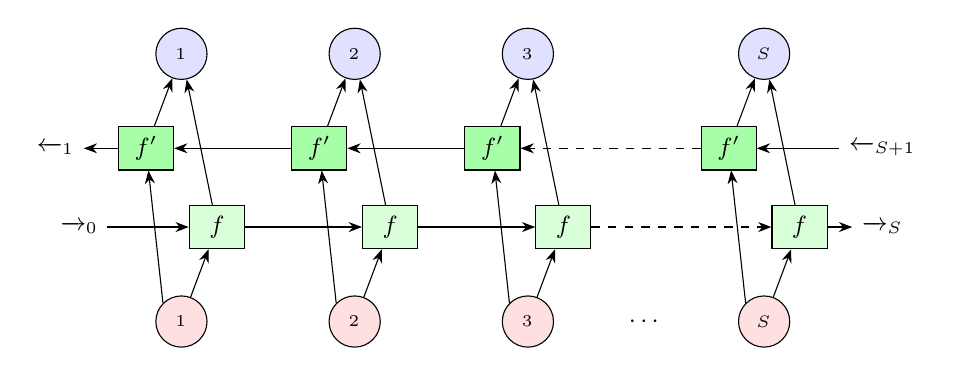
\begin{tikzpicture}[>=Stealth, every node/.style={font=\small},
      fw/.style={draw, fill=green!15, minimum width=0.7cm, minimum height=0.55cm},
      bw/.style={draw, fill=green!35, minimum width=0.7cm, minimum height=0.55cm},
      io/.style={draw, circle, minimum size=0.65cm, inner sep=0pt}]
    \foreach \i/\x in {1/0, 2/2.2, 3/4.4, S/7.4} {
      \node[io, fill=red!12] (x\i) at (\x,0) {$\vx_{\i}$};
      \node[fw] (f\i) at (\x+0.45,1.2) {$f$};
      \node[bw] (b\i) at (\x-0.45,2.2) {$f'$};
      \node[io, fill=blue!12] (y\i) at (\x,3.4) {$\vy_{\i}$};
      \draw[->] (x\i) -- (f\i); \draw[->] (x\i.north west) -- (b\i);
      \draw[->] (f\i) -- (y\i); \draw[->] (b\i) -- (y\i);
    }
    \node (dots) at (5.9,0) {$\cdots$};
    \node (h0) at (-1.3,1.2) {$\overrightarrow{\vh}_0$};
    \draw[->] (h0) -- (f1); \draw[->] (f1) -- (f2); \draw[->] (f2) -- (f3); \draw[->, dashed] (f3) -- (fS);
    \node (hS) at (8.9,1.2) {$\overrightarrow{\vh}_S$}; \draw[->] (fS) -- (hS);
    \node (b0) at (8.9,2.2) {$\overleftarrow{\vh}_{S+1}$};
    \draw[->] (b0) -- (bS); \draw[->, dashed] (bS) -- (b3); \draw[->] (b3) -- (b2); \draw[->] (b2) -- (b1);
    \node (b1out) at (-1.6,2.2) {$\overleftarrow{\vh}_1$}; \draw[->] (b1) -- (b1out);
  \end{tikzpicture}
  \caption{A bidirectional RNN. A forward RNN ($f$, light green) and a backward RNN ($f'$, dark green) each process the whole sequence; the output at each position combines the two states, and so depends on the inputs on both sides. For a single sequence-level prediction, the final states $\protect\overrightarrow{\vh}_S$ and $\protect\overleftarrow{\vh}_1$ are concatenated. After \citet{olah2015types}.}
  \label{fig:bidir}
\end{figure}

RNN layers can also be stacked: the sequence of hidden states of one layer, $\vh^{(1)}_1,\dots,\vh^{(1)}_S$, becomes the input sequence of the next. As in other deep networks, stacking lets higher layers build more abstract representations, and it is one way to increase capacity without increasing $K$.

%======================================================================
\section{Linear RNNs}
\label{sec:linear}
%======================================================================

\subsection{The parallelization problem}

RNNs went out of fashion for several years after transformers appeared (Chapter 3), largely for computational reasons. Computing $\vh_t$ requires $\vh_{t-1}$, so a layer cannot be evaluated at all positions at once; the forward and backward passes are \texttt{for} loops of length $S$. This makes poor use of GPUs, which are fast because they process many positions in parallel. A transformer layer computes all positions simultaneously during training, but at a cost quadratic in $S$. For DNA language models that aim to read hundreds of thousands to a million nucleotides at single-base resolution, neither a sequential loop of a million steps nor a quadratic attention matrix is attractive. \emph{Linear RNNs} offer a way out, and they are the basis of several recent DNA language models.

\subsection{Linear recurrences can be parallelized}

In a linear RNN the new state is a linear function of the old state, with coefficients that may depend on the input but not on the state,
\begin{equation}
  \vh_t = \va_t\odot\vh_{t-1} + \vbias_t ,
  \label{eq:linear_rnn}
\end{equation}
where $\va_t\in\R^K$ and $\vbias_t\in\R^K$ are (possibly nonlinear) functions of $\vx_t$ alone. Unrolling from $\vh_0=\mathbf{0}$,
\begin{equation}
  \vh_t = \sum_{s=1}^t\left(\prod_{r=s+1}^t\va_r\right)\odot\vbias_s ,
  \label{eq:linear_unrolled}
\end{equation}
with products taken elementwise and the empty product equal to $\vone$. Each step of~\eqref{eq:linear_rnn} is an affine map $\vh\mapsto\va_t\odot\vh+\vbias_t$, which we represent by the pair $(\va_t,\vbias_t)$. Applying $(\va,\vbias)$ and then $(\va',\vbias')$ gives $\vh\mapsto\va'\odot(\va\odot\vh+\vbias)+\vbias' = (\va'\odot\va)\odot\vh + (\va'\odot\vbias+\vbias')$, so composition is the operation
\begin{equation}
  (\va,\vbias)\bullet(\va',\vbias') = \left(\va\odot\va',\ \va'\odot\vbias+\vbias'\right).
\end{equation}
Composition of functions is associative, so $\bullet$ is associative, and $\vh_t$ is the second component of $(\va_1,\vbias_1)\bullet\cdots\bullet(\va_t,\vbias_t)$. Computing all such prefix products is a \emph{prefix scan}, which can be done with $O(S)$ total work in $O(\log S)$ parallel steps, for example by combining adjacent pairs, then adjacent pairs of pairs, and so on~\citep{blelloch1990,martin2018}. The nonlinear RNNs of the previous sections do not have this property, because $\va_t$ and $\vbias_t$ would depend on $\vh_{t-1}$.

When the coefficient $\va_t=\va$ is the same at every position and $\vbias_t=\mathbf{B}\vx_t$ is a linear function of the input, with $\mathbf{B}\in\R^{K\times P}$, \eqref{eq:linear_unrolled} becomes $\vh_t=\sum_{k=0}^{t-1}\va^k\odot\mathbf{B}\vx_{t-k}$, a convolution of the input with a long, exponentially decaying filter. This connects linear RNNs to the long convolutions of structured state space models~\citep{gu2022} and the Hyena operator~\citep{poli2023}: the same model can be trained as a parallel convolution or scan and run at inference time as a recurrence, with constant memory per step.

The gradient of a linear RNN is also well behaved. From~\eqref{eq:linear_rnn}, $\partial\vh_t/\partial\vh_{t-1}=\diag(\va_t)$, the direct path of the GRU and LSTM without the other terms. If the entries of $\va_t$ are kept in $(0,1)$, for example by a sigmoid, the gradient cannot explode, and it is preserved wherever $\va_t$ is close to 1.

\subsection{A minimal GRU}

Removing the dependence of the GRU's gates and candidate on $\vh_{t-1}$ gives a linear RNN. The minimal GRU~\citep{feng2024} uses
\begin{equation}
  \vz_t = \sigma(\mW_z\vx_t+\vbias_z), \qquad \tilde\vg_t = \mW_g\vx_t+\vbias_g, \qquad
  \vh_t = (\vone-\vz_t)\odot\vh_{t-1} + \vz_t\odot\tilde\vg_t ,
\end{equation}
which is~\eqref{eq:linear_rnn} with $\va_t=\vone-\vz_t$ and $\vbias_t=\vz_t\odot\tilde\vg_t$. A single such layer is less expressive than a GRU, since the state cannot influence what is written into it. Stacking layers, with nonlinear dense layers in between, restores much of the expressiveness while keeping every layer parallelizable. The trade-off is captured by the slogan ``not quite as expressive, but fully parallelizable''.

\subsection{Linear RNNs for DNA}

Several recent sequence models build on this idea. Mamba~\citep{gu2023} is a selective state space model: a linear recurrence whose coefficients depend on the input, so that, like a gate, the model can choose at each position what to remember and what to ignore, implemented with a hardware-aware parallel scan. HyenaDNA~\citep{nguyen2023} uses the Hyena operator, which interleaves implicitly parameterized long convolutions with elementwise gating, to model up to a million nucleotides at single-nucleotide resolution. Caduceus~\citep{schiff2024} extends Mamba blocks to be bidirectional and equivariant to reverse complementation, so that a sequence and its reverse complement, the same DNA read from the other strand, receive consistent representations. Evo~\citep{nguyen2024} uses a hybrid architecture that interleaves Hyena layers with attention layers; similar hybrids of linear recurrences and attention are used in general-purpose language models such as RecurrentGemma~\citep{botev2024}. Hybrids aim to combine the efficiency of linear recurrences on very long sequences with the accuracy of attention.

Figure~\ref{fig:mamba_scaling} compares these architectures as DNA language models, trained to predict the next nucleotide on the human reference genome. Performance is measured by \emph{perplexity}, the exponential of the average per-nucleotide cross-entropy, $\exp\left(-\frac{1}{S}\sum_t\log p(s_t\mid s_{1:t-1})\right)$. A model that guesses uniformly among the four nucleotides has perplexity 4, and a perfect model has perplexity 1. All three architectures improve with size, with Mamba the best at each size in this comparison. That even the largest models remain well above 2 shows how hard it is to predict the next nucleotide of the genome. Whether DNA language models trained this way learn biology that is useful for downstream tasks is still an open question.

\begin{figure}[t]
  \centering
  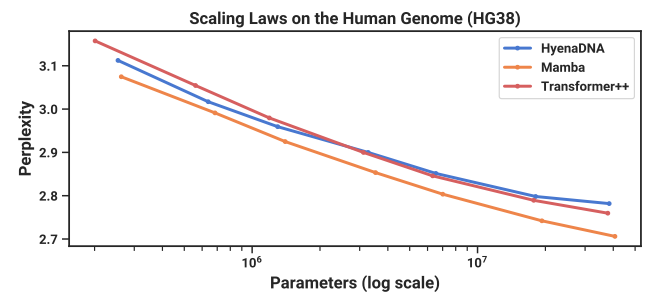
\includegraphics[width=0.65\linewidth]{slides/mamba_dna_scaling.png}
  \caption{Next-nucleotide perplexity on the human genome (HG38) against model size for a transformer (Transformer++), HyenaDNA and Mamba. Lower is better. Reproduced from \citet{gu2023}.}
  \label{fig:mamba_scaling}
\end{figure}

%======================================================================
\section{DNA methylation}
\label{sec:methylation}
%======================================================================

\subsection{Methylated cytosine}

Chapter 3 introduced histone modifications, chemical groups such as methyl or acetyl groups attached to the tails of the histone proteins around which DNA is wrapped; H3K27me3, for example, is three methyl groups on lysine 27 of histone H3. \emph{DNA methylation} is a modification of the DNA itself. In mammals, and most other vertebrates, it is the addition of a methyl group to carbon 5 of a cytosine, giving 5-methylcytosine (5mC; Figure~\ref{fig:methyl_cycle}), almost always at a cytosine followed by a guanine. Such a dinucleotide is written CpG, where the ``p'' denotes the phosphate linking the two nucleotides along one strand and distinguishes it from a C--G base pair across the two strands. CpG is its own reverse complement, so a CpG on one strand faces a CpG on the other, and methylation is usually symmetric: both cytosines are methylated, or neither is. In somatic human cells around 70--80\% of CpGs are methylated~\citep{jones2012}.

\begin{figure}[t]
  \centering
  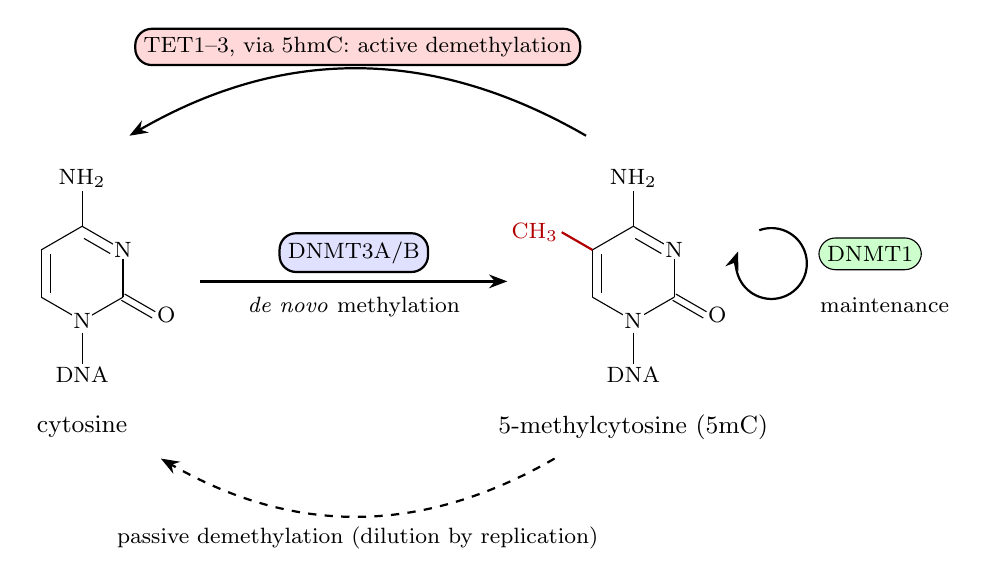
\begin{tikzpicture}[>=Stealth, every node/.style={font=\small},
      atom/.style={fill=white, inner sep=0.5pt, font=\footnotesize},
      enz/.style={draw, rounded corners=6pt, inner sep=3pt, font=\footnotesize}]
    \tikzset{ring/.pic={
      \foreach \a/\b in {90/30, 30/-30, -30/-90, -90/-150, -150/150, 150/90} \draw (\a:0.6) -- (\b:0.6);
      \draw ($(90:0.6)!0.18!(30:0.6)+(-0.07,-0.1)$) -- ($(90:0.6)!0.82!(30:0.6)+(-0.07,-0.1)$);
      \draw ($(-150:0.6)+(0.12,0.05)$) -- ($(150:0.6)+(0.12,-0.05)$);
      \node[atom] at (30:0.6) {N};
      \node[atom] at (-90:0.6) {N};
      \draw (90:0.6) -- (90:1.05) node[above, inner sep=1pt, font=\footnotesize] {NH$_2$};
      \draw ($(-30:0.6)+(0.02,0.04)$) -- ($(-30:1.05)+(0.02,0.04)$);
      \draw ($(-30:0.6)+(-0.02,-0.04)$) -- ($(-30:1.05)+(-0.02,-0.04)$);
      \node[right, inner sep=1pt, font=\footnotesize] at (-30:1.05) {O};
      \draw (-90:0.75) -- (-90:1.15) node[below, inner sep=1pt, font=\footnotesize] {DNA};
    }}
    \pic at (0,0) {ring};
    \node at (0,-1.95) {cytosine};
    \pic at (7,0) {ring};
    \draw[red!70!black, thick] (7,0) ++(150:0.6) -- ++(150:0.45) node[left, inner sep=1pt, font=\footnotesize] {CH$_3$};
    \node at (7,-1.95) {5-methylcytosine (5mC)};
    \draw[->, thick] (1.5,-0.1) -- node[above=3pt, enz, fill=blue!12] {DNMT3A/B} node[below=2pt, font=\footnotesize] {\textit{de novo} methylation} (5.4,-0.1);
    \draw[->, thick] (6.4,1.75) to[out=150, in=30] node[above=1pt, enz, fill=red!15] {TET1--3, via 5hmC: active demethylation} (0.6,1.75);
    \draw[->, thick, dashed] (6.0,-2.35) to[out=-150, in=-30] node[below, font=\footnotesize] {passive demethylation (dilution by replication)} (1.0,-2.35);
    \draw[->, thick] (8.6,0.55) arc[start angle=110, end angle=-200, radius=0.45];
    \node[enz, fill=green!20, right] at (9.35,0.25) {DNMT1};
    \node[right, font=\footnotesize] at (9.25,-0.4) {maintenance};
  \end{tikzpicture}
  \caption{DNA methylation adds a methyl group (red) to carbon 5 of cytosine. DNMT3A and DNMT3B establish new methylation; DNMT1 copies existing methylation to the new strand after DNA replication. Methylation is removed actively, by TET enzymes that oxidize 5mC to 5-hydroxymethylcytosine (5hmC) and further products that are excised and replaced, or passively, when maintenance fails and methylation is diluted over cell divisions.}
  \label{fig:methyl_cycle}
\end{figure}

\subsection{Writing, maintaining and erasing methylation}

The enzymes that place methyl groups are DNA methyltransferases (DNMTs; Figure~\ref{fig:methyl_cycle}). DNMT3A and DNMT3B establish methylation at previously unmethylated sites (\emph{de novo} methylation), for example during early development~\citep{okano1999}. When DNA is replicated, each daughter molecule has one old, methylated strand and one new, unmethylated strand. DNMT1 recognizes these hemimethylated CpGs and methylates the new strand, which is how methylation patterns are \emph{maintained} through cell division. This copying mechanism makes DNA methylation a heritable, relatively stable mark, part of the cell's \emph{epigenetic} memory. Methylation can be lost passively, when DNMT1 does not act and the mark is diluted over successive divisions, or actively, by the TET enzymes, which oxidize 5mC to 5-hydroxymethylcytosine (5hmC) and further products that DNA repair then replaces with unmodified cytosine~\citep{tahiliani2009}.

\subsection{CpG islands and gene regulation}

CpGs are rare in mammalian genomes, occurring at about a quarter of the frequency expected from the frequencies of C and G~\citep{bird1980}. The reason is mutation. Cytosines spontaneously lose their amino group (deamination). Unmethylated cytosine deaminates to uracil, which does not belong in DNA and is efficiently repaired. Methylated cytosine deaminates to thymine, giving a T:G mismatch that is repaired less reliably, so methylated CpGs mutate to TpG (and, on the other strand, to CpA) at a high rate. Over evolutionary time this has depleted CpGs from the methylated majority of the genome, and CpG-to-TpG transitions remain among the most frequent mutations in human populations and in cancers.

The exceptions are \emph{CpG islands}, stretches of a few hundred to a few thousand base pairs with high GC content and close to the expected CpG frequency (a common working definition is at least 200 bp, GC content above 50\% and an observed-to-expected CpG ratio above 0.6~\citep{gardinergarden1987}). There are roughly 25{,}000 to 30{,}000 CpG islands in the human genome, similar to the number of genes, and about 70\% of gene promoters overlap one~\citep{saxonov2006}. Most CpG islands are unmethylated in most cells, which is why they have escaped CpG depletion (Figure~\ref{fig:cpg_island}).

\begin{figure}[t]
  \centering
  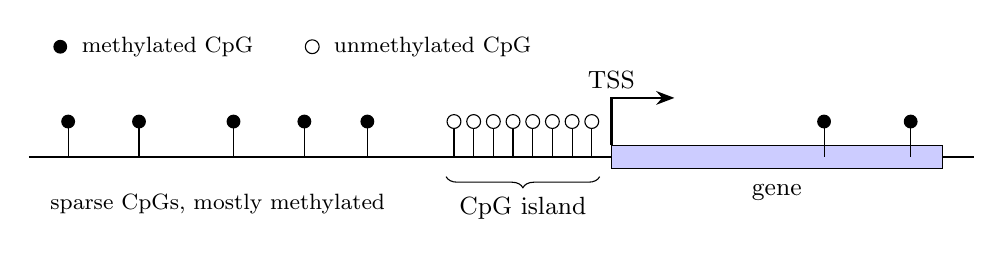
\begin{tikzpicture}[>=Stealth, every node/.style={font=\small}]
    \draw[thick] (0,0) -- (12,0);
    \draw[fill=blue!20] (7.4,-0.15) rectangle (11.6,0.15);
    \node at (9.5,-0.45) {gene};
    \draw[->, thick] (7.4,0.15) -- (7.4,0.75) -- (8.2,0.75);
    \node[above] at (7.4,0.75) {TSS};
    % flanking methylated CpGs
    \foreach \x in {0.5, 1.4, 2.6, 3.5, 4.3, 10.1, 11.2} {
      \draw (\x,0) -- (\x,0.45); \fill (\x,0.45) circle (2.5pt);
    }
    % island unmethylated CpGs
    \foreach \x in {5.4,5.65,5.9,6.15,6.4,6.65,6.9,7.15} {
      \draw (\x,0) -- (\x,0.45); \draw[fill=white] (\x,0.45) circle (2.5pt);
    }
    \draw[decorate, decoration={brace, mirror, amplitude=4pt}] (5.3,-0.25) -- (7.25,-0.25) node[midway, below=4pt, align=center] {CpG island};
    \node[align=center, font=\footnotesize] at (2.4,-0.6) {sparse CpGs, mostly methylated};
    \fill (0.4,1.4) circle (2.5pt); \node[right, font=\footnotesize] at (0.55,1.4) {methylated CpG};
    \draw[fill=white] (3.6,1.4) circle (2.5pt); \node[right, font=\footnotesize] at (3.75,1.4) {unmethylated CpG};
  \end{tikzpicture}
  \caption{Most CpGs in the genome are sparse and methylated. CpG islands, dense clusters of CpGs, often overlap promoters near the transcription start site (TSS) and are usually unmethylated when the gene is active.}
  \label{fig:cpg_island}
\end{figure}

DNA methylation at promoters is associated with repression of transcription. If a gene is active in a cell type, its promoter CpG island tends to be unmethylated, and across cell types the methylation of a promoter island is strongly anticorrelated with the expression of its gene. Methylated promoter islands are associated with stable, long-term silencing, as on the inactive X chromosome and at imprinted genes~\citep{deaton2011,jones2012}. The mechanisms are still being worked out. One is that many transcription factors, which more often activate than repress transcription, bind methylated DNA less well than unmethylated DNA, although some prefer methylated sites~\citep{yin2017}. Another is crosstalk with the chromatin marks of Chapter 3: DNA methylation and histone modifications influence each other, so that methylation can affect transcription indirectly, and which comes first is not always clear. Methylation in gene bodies, in contrast, tends to be positively correlated with expression~\citep{jones2012}. Together, transcription factor binding, chromatin accessibility, histone modifications and DNA methylation interact to let each cell type express its own set of genes.

DNA methylation also changes with age, consistently enough to serve as a molecular clock. \citet{horvath2013} fit an elastic net, the combination of ridge and lasso penalties from Chapter 1, to predict chronological age from methylation array data and obtained a predictor based on 353 CpGs that is accurate across many tissues. Such ``epigenetic clocks'' are now widely used as biomarkers of biological ageing.

\subsection{Measuring methylation by bisulfite sequencing}

Methylation can be measured with microarrays, which probe a predefined set of hundreds of thousands of CpGs and have been used in large population cohorts, or by sequencing. The standard sequencing approach relies on the chemistry of \emph{sodium bisulfite}~\citep{frommer1992}. Bisulfite treatment converts unmethylated cytosine to uracil, but leaves 5mC unchanged. During amplification and sequencing, uracil is read as thymine. After treatment, a methylated CpG therefore still reads as CpG, while an unmethylated CpG reads as TpG (Figure~\ref{fig:bisulfite}). The reads are aligned to the reference genome with an aligner that allows for these conversions, such as Bismark~\citep{krueger2011}. At each CpG, a read showing C indicates methylation and a read showing T indicates its absence. Cytosines outside CpG context are almost all unmethylated in somatic cells, so their conversion rate measures how complete the bisulfite reaction was. Bisulfite treatment does not distinguish 5mC from 5hmC; variants such as oxidative bisulfite sequencing separate the two~\citep{booth2012}.

\begin{figure}[t]
  \centering
  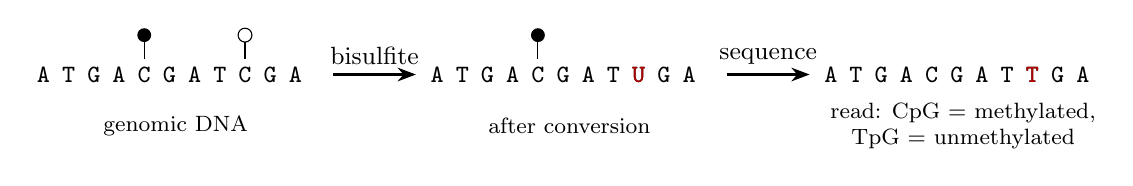
\begin{tikzpicture}[>=Stealth, every node/.style={font=\ttfamily\small}]
    \def\seqA{A,T,G,A,C,G,A,T,C,G,A}
    \def\seqB{A,T,G,A,C,G,A,T,U,G,A}
    \def\seqC{A,T,G,A,C,G,A,T,T,G,A}
    \foreach \c [count=\i] in \seqA \node at (0.32*\i,0) {\c};
    \foreach \c [count=\i] in \seqB \node at (0.32*\i+5,0) {\c};
    \foreach \c [count=\i] in \seqC \node at (0.32*\i+10,0) {\c};
    \foreach \off in {0,5} { \draw (0.32*5+\off,0.2) -- (0.32*5+\off,0.5); \fill (0.32*5+\off,0.5) circle (2.5pt); }
    \draw (0.32*9,0.2) -- (0.32*9,0.5); \draw[fill=white] (0.32*9,0.5) circle (2.5pt);
    \draw[->, thick] (4.0,0) -- node[above, font=\small\rmfamily] {bisulfite} (5.05,0);
    \draw[->, thick] (9.0,0) -- node[above, font=\small\rmfamily] {sequence} (10.05,0);
    \node[red!70!black] at (0.32*9+5,0) {U};
    \node[red!70!black] at (0.32*9+10,0) {T};
    \node[font=\footnotesize\rmfamily, align=center] at (2.0,-0.65) {genomic DNA};
    \node[font=\footnotesize\rmfamily, align=center] at (7.0,-0.65) {after conversion};
    \node[font=\footnotesize\rmfamily, align=center] at (12.0,-0.65) {read: CpG = methylated,\\TpG = unmethylated};
  \end{tikzpicture}
  \caption{Bisulfite sequencing. Of the two CpGs, the first is methylated (filled circle) and the second is not (open circle). Bisulfite converts the unmethylated cytosine to uracil, which is read as thymine; the methylated cytosine is protected. Aligned to the reference, the unmethylated site looks like a C-to-T substitution.}
  \label{fig:bisulfite}
\end{figure}

Bisulfite-induced C-to-T changes resemble real mutations, and also the DNA damage seen in ancient DNA: in fragments recovered from Neanderthal remains, cytosine deamination produces an excess of apparent C-to-T substitutions, especially near the ends of molecules~\citep{briggs2007}.

\emph{Whole-genome bisulfite sequencing} (WGBS) applies this to the entire genome~\citep{lister2009}. Because the genome is mostly CpG-poor, much of the sequencing is spent on regions with few CpGs. \emph{Reduced representation bisulfite sequencing} (RRBS)~\citep{meissner2005} first digests the DNA with the restriction enzyme MspI, which cuts at CCGG, and selects short fragments. This enriches for CpG-dense regions such as CpG islands and promoters, giving deeper coverage of a small, CpG-rich fraction of the genome at lower cost.

\subsection{From read counts to methylation levels}
\label{sec:read_counts}

In a bulk sample, a CpG is covered by $n$ reads from different cells, $m$ of which show C. The methylation level $q\in[0,1]$, the fraction of DNA copies methylated at that site, is estimated by $\hat q=m/n$. Modelling $m\mid q\sim\text{Binomial}(n,q)$ with a uniform prior on $q$, the posterior is $q\mid m\sim\text{Beta}(1+m,1+n-m)$, whose width shrinks roughly as $1/\sqrt{n}$ (Figure~\ref{fig:meth_post}). Deep bulk sequencing gives nearly continuous, precise estimates. In a single cell there are only two copies of each CpG (one per homologous chromosome), and in practice a CpG is covered by at most one or two reads, so each observation is essentially binary, and most CpGs are not observed at all. Single-cell bisulfite sequencing (scBS-seq)~\citep{smallwood2014} covers on the order of 20--40\% of CpGs per cell, and single-cell RRBS 1--10\%~\citep{angermueller2017}. To say anything about an unobserved site we must borrow information from neighbouring CpGs, from other cells and from the DNA sequence, which is the problem addressed next.

\begin{figure}[t]
  \centering
  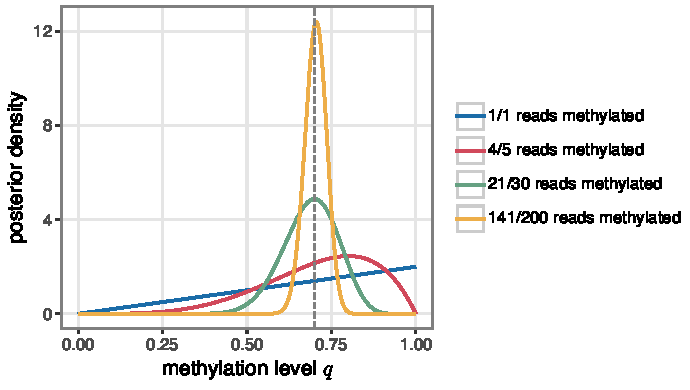
\includegraphics[width=0.65\linewidth]{methylation_posterior.pdf}
  \caption{Posterior distribution of the methylation level $q$ of a CpG under a uniform prior, given $m$ methylated reads out of $n$, for data generated with $q=0.7$ (dashed line). One read, as in single-cell data, barely constrains $q$; hundreds of reads, as in deep bulk sequencing, pin it down.}
  \label{fig:meth_post}
\end{figure}

%======================================================================
\section{Application: imputing single-cell methylation with DeepCpG}
\label{sec:deepcpg}
%======================================================================

\subsection{The data and the task}

Single-cell methylation data can be arranged as a matrix with one row per cell and one column per CpG site, with entries 1 (methylated), 0 (unmethylated) or missing (Figure~\ref{fig:deepcpg}, left). Let $N$ be the number of cells and $M$ the number of CpG sites, $y_{ni}\in\{0,1\}$ the methylation state of site $i$ in cell $n$, and $o_{ni}\in\{0,1\}$ an indicator that it was observed. Most entries are missing. DeepCpG~\citep{angermueller2017} predicts the methylation state of every site in every cell, imputing the missing entries, from two sources of information: the DNA sequence around the site, and the observed methylation states at neighbouring sites in the same cell and in other cells. Holding out an observed site and predicting it from its context is similar in spirit to masked language modelling.

\begin{figure}[t]
  \centering
  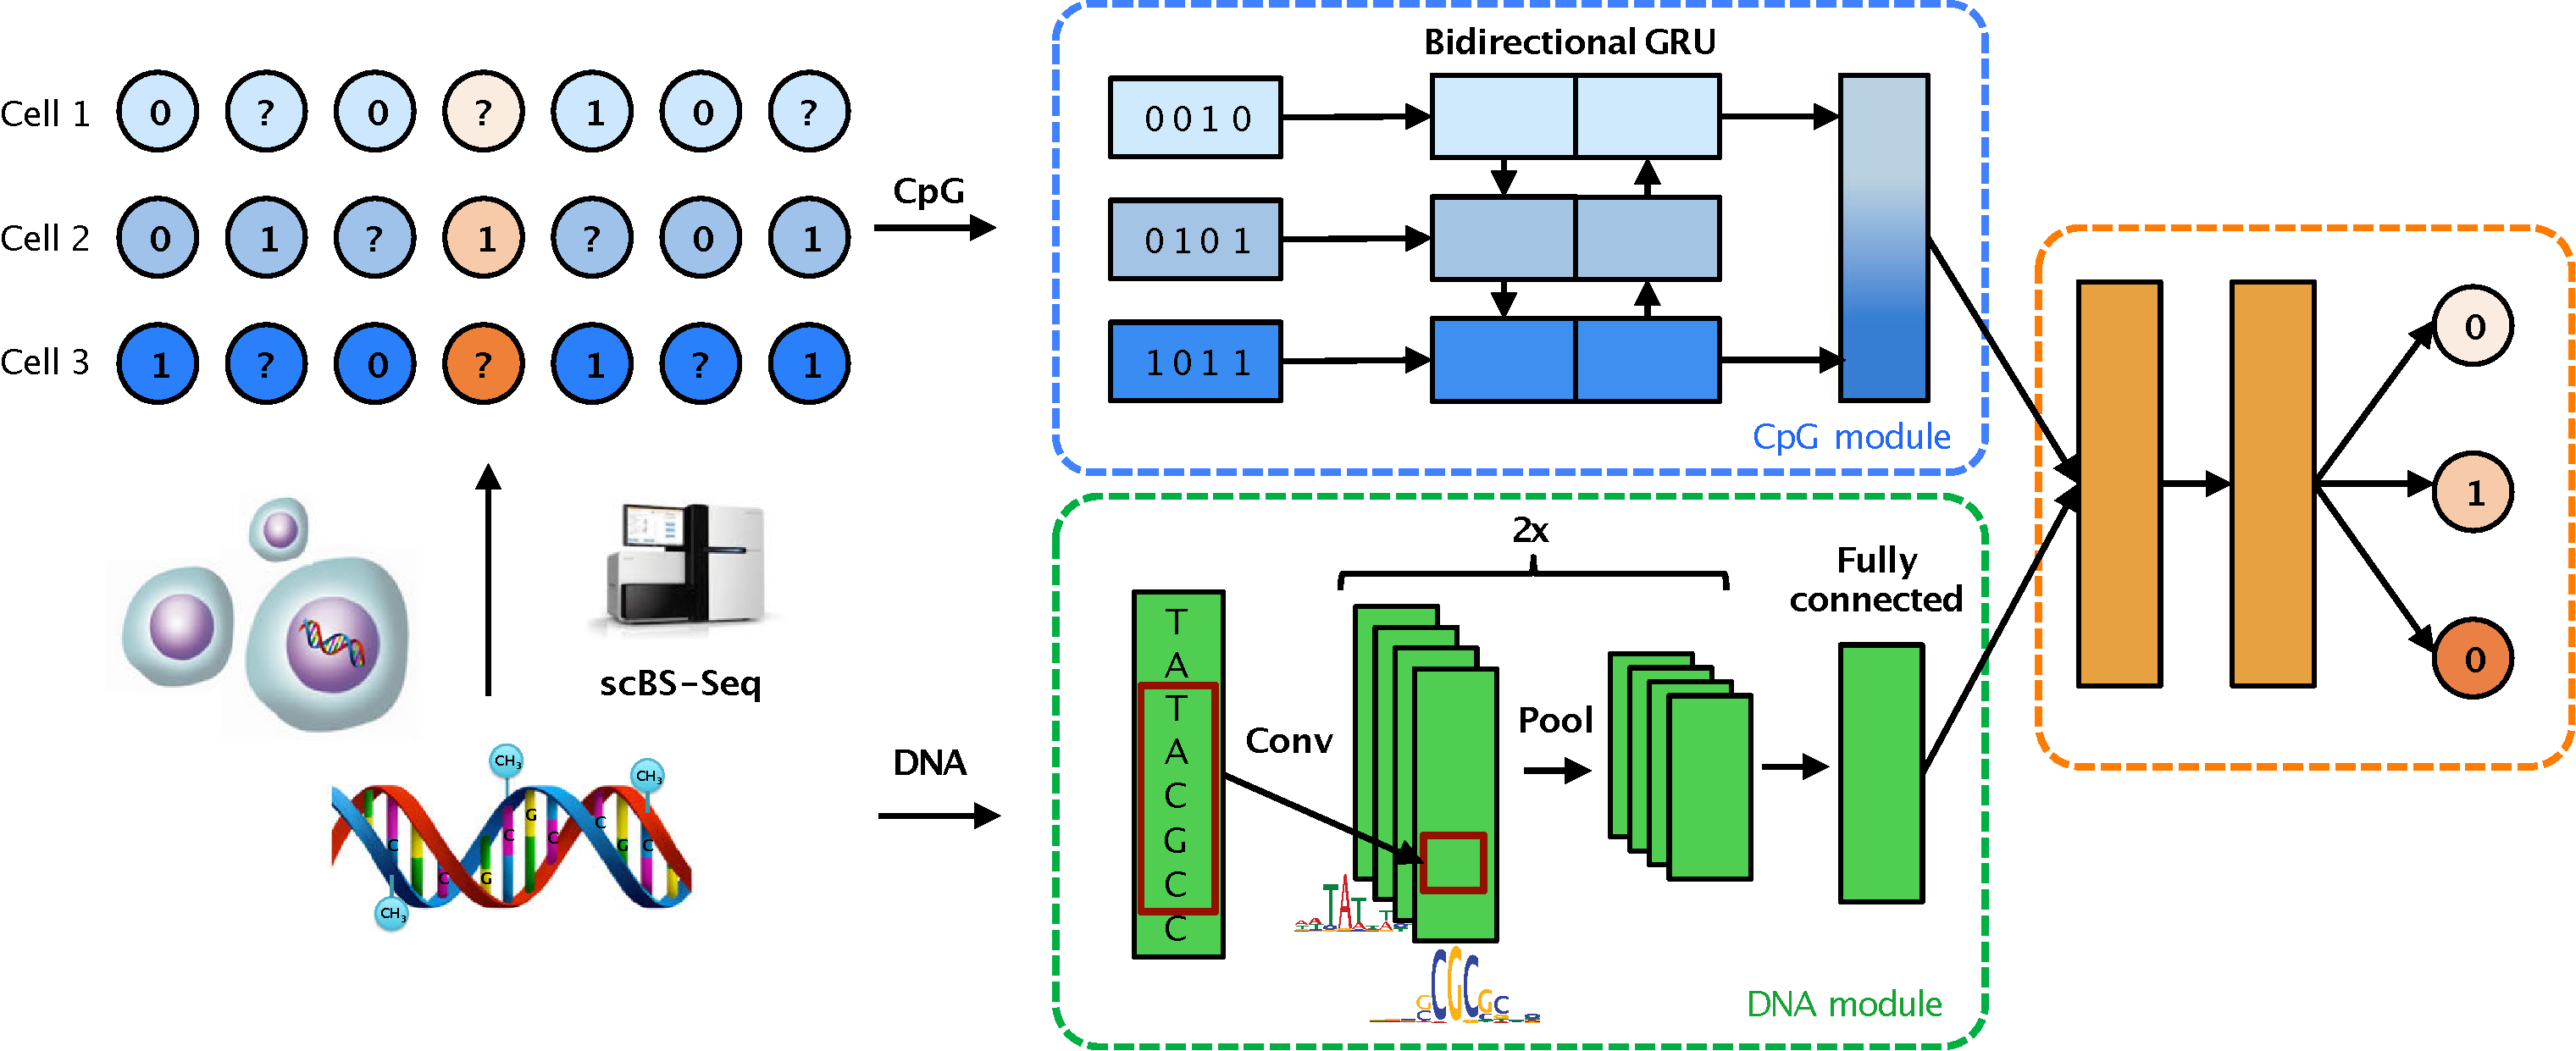
\includegraphics[width=\linewidth]{slides/deepcpg_architecture.pdf}
  \caption{DeepCpG. Left, single-cell bisulfite sequencing gives a sparse binary matrix of methylation states (cells $\times$ CpG sites; ``?'' marks unobserved sites). The CpG module (blue) summarizes the observed states near the target site in each cell and combines cells with a bidirectional GRU. The DNA module (green) is a CNN on the sequence window around the target site. The joint module (orange) combines the two and predicts the methylation state of the target site in every cell. Reproduced from \citet{angermueller2017} (CC BY 4.0).}
  \label{fig:deepcpg}
\end{figure}

\subsection{The model}

DeepCpG has three modules (Figure~\ref{fig:deepcpg}).
\begin{itemize}
  \item The \emph{DNA module} is a CNN of the kind described in Chapter 2. Its input is the one-hot encoded 1001 bp window centred on the target CpG, a $1001\times4$ matrix. Two or three convolution and max-pooling layers, followed by a dense layer, map it to a feature vector.
  \item The \emph{CpG module} uses the observed methylation states around the target site. For each cell $n$ it forms a vector $\mathbf{v}_n\in\R^{100}$ containing the states of, and distances to, the 25 nearest observed CpGs on each side of the target site in that cell. A dense layer embeds each $\mathbf{v}_n$ into $\R^{256}$, capturing patterns within the cell. A bidirectional GRU then runs over the sequence of embedded vectors for cells $1,\dots,N$, and the final states of the two directions are concatenated into a vector in $\R^{512}$, capturing patterns across cells.
  \item The \emph{joint module} concatenates the outputs of the DNA and CpG modules and passes them through two dense layers of 512 ReLU units. Its output layer has one sigmoid unit per cell, giving predicted probabilities $\hat y_{ni}\in(0,1)$ that site $i$ is methylated in cell $n$, so the model is multitask in the sense of Chapter 2.
\end{itemize}
Note that the recurrence in the CpG module runs over cells, not along the genome. The order of the CpGs along the genome is encoded within each cell's input vector $\mathbf{v}_n$, through the states and distances of the neighbouring sites. The GRU is used to compress a variable number of cells into a fixed-length vector; running it in both directions reduces the dependence of this summary on the arbitrary order in which cells are listed.

The model is trained by minimizing the cross-entropy over observed entries only, with an L2 penalty on the weights $\vtheta$,
\begin{equation}
  L(\vtheta) = -\sum_{i=1}^M\sum_{n=1}^N o_{ni}\left[y_{ni}\log\hat y_{ni} + (1-y_{ni})\log(1-\hat y_{ni})\right] + \lambda\|\vtheta\|_2^2 .
\end{equation}
Unobserved entries contribute nothing to the loss, so missing data need no special treatment during training, and at prediction time the model produces $\hat y_{ni}$ for every entry. The DNA and CpG modules were first trained separately and then held fixed while the joint module was trained. Training, validation and test sets were whole chromosomes, so that test sites are not near training sites, which would otherwise share sequence context and neighbouring methylation states.

\subsection{Results}

The main data set was 18 mouse embryonic stem cells profiled by scBS-seq, with an average of 17.7\% of CpGs observed per cell, and the model was also applied to scRRBS-seq data from human and mouse cells~\citep{angermueller2017}. DeepCpG predicted held-out methylation states more accurately, measured by AUROC, than random forests using the same inputs or genome annotations, and than simple baselines that average observed states in a window of the same cell or at the same site across other cells (Figure~\ref{fig:deepcpg_results}a). Neighbouring methylation states were more predictive than DNA sequence, and combining the two was best.

\begin{figure}[t]
  \centering
  \begin{subfigure}[b]{0.46\linewidth}
    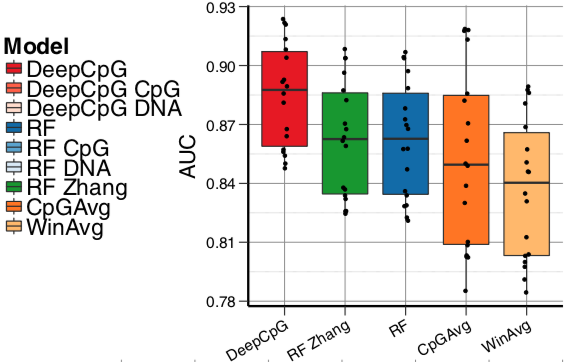
\includegraphics[width=\linewidth]{slides/deepcpg_auc.png}
    \caption{}
  \end{subfigure}\hfill
  \begin{subfigure}[b]{0.5\linewidth}
    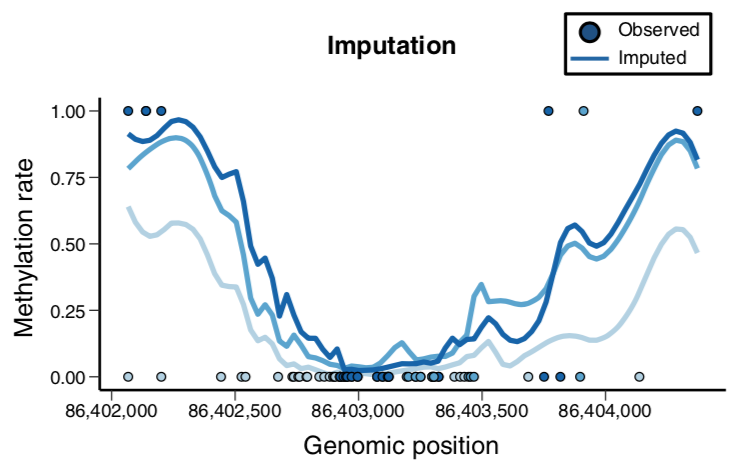
\includegraphics[width=\linewidth]{slides/deepcpg_imputation.png}
    \caption{}
  \end{subfigure}
  \begin{subfigure}[b]{0.8\linewidth}
    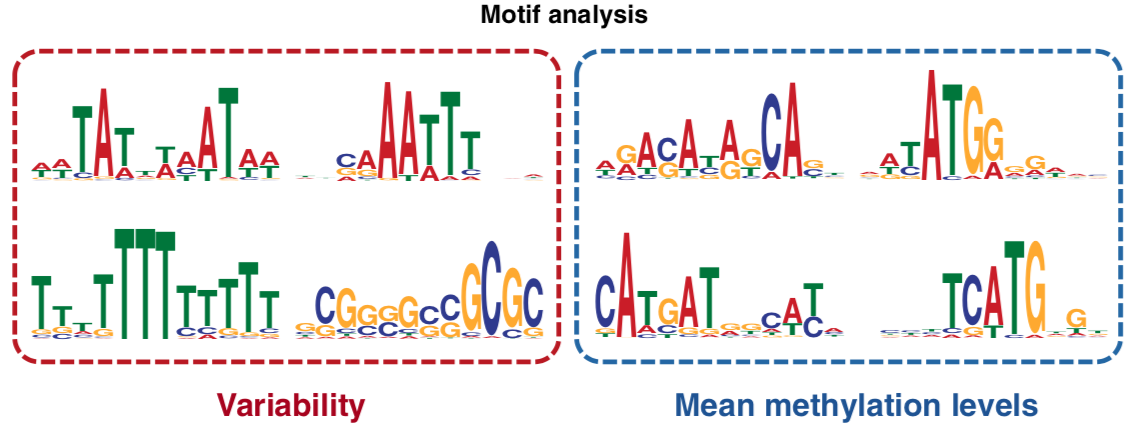
\includegraphics[width=\linewidth]{slides/deepcpg_motifs.png}
    \caption{}
  \end{subfigure}
  \caption{DeepCpG results. (a) AUROC for predicting held-out methylation states, one point per cell, for DeepCpG, random forests using annotations (RF Zhang) or the same inputs as DeepCpG (RF), and averaging across cells (CpGAvg) or within a window (WinAvg). (b) Observed states (points, at 0 or 1) and imputed methylation probabilities (lines) for three cells, shown in different shades, across a region of about 2.5 kb containing a CpG island, where observed CpGs are dense and methylation is low. (c) Examples of first-layer convolutional filters, displayed as sequence logos, associated with cell-to-cell variability in methylation (left) or with mean methylation level (right). Reproduced from \citet{angermueller2017} (CC BY 4.0).}
  \label{fig:deepcpg_results}
\end{figure}

Figure~\ref{fig:deepcpg_results}b shows imputed profiles for three cells across a CpG island. The observations are binary and sparse, but the imputed probabilities are smooth and low across the island, where CpGs are dense, and high on the flanks, with differences between cells. As with the CNNs of Chapters 2 and 3, the first-layer filters of the DNA module can be visualized as sequence logos (Figure~\ref{fig:deepcpg_results}c). Some matched known transcription factor motifs. CG-rich motifs tended to be associated with low methylation and AT-rich motifs with high methylation. To separate motifs that affect the average methylation level from those that affect variability between cells, the authors trained a second network with the same DNA module to predict both the mean and the cell-to-cell variance of methylation in windows around each site.

Like ChromHMM in Chapter 6, DeepCpG looks at epigenomic data at many positions along the genome and in many samples, and exploits the dependence between nearby positions and between samples to find structure. The difference is that ChromHMM is an unsupervised model of chromatin states, while DeepCpG is trained in a supervised way to predict held-out observations.

%======================================================================
\section{RNNs and hidden Markov models}
\label{sec:rnn_hmm}
%======================================================================

RNNs can be thought of as the deep learning version of hidden Markov models, and the analogy is close. Recall the forward pass of Chapter 6. For an HMM with $K$ states, transition matrix $\mT\in\R^{K\times K}$ and emission likelihoods $\mathbf{e}_t\in\R^K$, $e_t(i)=P(y_t\mid X_t=i)$ (written $\vphi_t$ in Chapter 6), the filtered state probabilities $\vf_t\in\R^K$, $f_t(i)=P(X_t=i\mid y_{1:t})$ (not to be confused with the LSTM forget gate), satisfy
\begin{equation}
  \vf_t = \frac{\mathbf{e}_t\odot(\mT^\top\vf_{t-1})}{\vone^\top\left(\mathbf{e}_t\odot(\mT^\top\vf_{t-1})\right)} .
\end{equation}
This is an RNN with hidden state $\vf_t$: a fixed linear map of the previous state, multiplied elementwise by a vector that depends on the current observation, and normalized. Before normalization it is even a linear RNN in the sense of Section~\ref{sec:linear}, with an input-dependent gate $\mathbf{e}_t$ (though with a full matrix $\mT$ rather than a diagonal one). The backward pass is a second recurrence running in the opposite direction, and combining the two to compute posterior marginals corresponds to a bidirectional RNN. The differences lie in what the state represents and how the model is fit. The HMM state vector is a probability distribution over a small number of interpretable discrete states, the model is generative and is fit by maximum likelihood with EM, and its recurrence is fixed by the probabilistic model. The RNN state is an unconstrained continuous vector, the recurrence is a learned nonlinear function, and the model is usually trained discriminatively by gradient descent. The RNN is therefore more flexible, at the cost of interpretability and of the probabilistic guarantees that come with the HMM.

%======================================================================
\section{Summary}
%======================================================================

\begin{itemize}
  \item RNNs process a sequence by applying the same small network at every position, carrying a hidden state $\vh_t=f_{\mW}(\vh_{t-1},\vx_t)$. They handle variable input and output lengths, can in principle carry information over long distances, and are naturally causal, which suits autoregressive modelling. They are the deep learning analogue of HMMs.
  \item The vanilla RNN is trained by backpropagation through time, which multiplies the gradient by the same matrix $\mW_h$ at every step. The gradient therefore vanishes or explodes exponentially with distance, depending on the singular values of $\mW_h$.
  \item Gated units fix this by making the step-to-step dependence data-adaptive. The GRU interpolates between the old state and a candidate with an update gate; the LSTM keeps a separate cell state controlled by input, forget and output gates. Gradients flow along the gated direct path without repeated multiplication by the same matrix.
  \item Bidirectional RNNs combine a forward and a backward pass so that each position sees the whole sequence. Linear RNNs, whose state update is linear in the previous state, can be computed in parallel with a prefix scan; they underlie DNA language models such as HyenaDNA, Mamba-based Caduceus and hybrid models such as Evo.
  \item DNA methylation of cytosines at CpGs is a heritable epigenetic mark, generally low in active promoter CpG islands and associated with repression. Bisulfite sequencing measures it by converting unmethylated cytosines, which are then read as thymines. Single-cell data are binary and sparse, and DeepCpG imputes them by combining a CNN on DNA sequence with a bidirectional GRU that pools neighbouring methylation states across cells.
\end{itemize}

%======================================================================
\section*{Exercises}
%======================================================================

\begin{enumerate}
  \item Derive the GRU Jacobian~\eqref{eq:gru_jac}. Show that if $z_{tk}\to0$ for all $k$, then $\partial\vh_t/\partial\vh_{t-1}\to\mI$, and that if $z_{tk}\to1$ for all $k$, the Jacobian approaches $\diag(\vone-\vg_t\odot\vg_t)\diag(\vr_t)\mW_h$ plus a term involving the reset gate. Interpret the two limits.
  \item For the LSTM~\eqref{eq:lstm}, write $\partial\vc_t/\partial\vc_{t-1}$ including the dependence of the gates on $\vh_{t-1}=\vo_{t-1}\odot\tanh(\vc_{t-1})$. Under what conditions on the gates is the additional term small?
  \item Show that the operation $\bullet$ of Section~\ref{sec:linear} is associative. For $S=8$, write out the steps of a parallel prefix scan that computes $\vh_1,\dots,\vh_8$, and count the number of sequential steps and of applications of $\bullet$.
  \item Implement a vanilla RNN and a GRU, with the same hidden dimension, for a synthetic task: given a random DNA sequence of length $S$, predict its first nucleotide from the final hidden state. Plot test accuracy against $S$ for each model. Repeat with gradient clipping for the vanilla RNN.
  \item Under the binomial model of Section~\ref{sec:read_counts} with a uniform prior, find the posterior mean of $q$ after a single read showing C. Suppose instead that $q$ is shared by $J$ neighbouring CpGs in the same cell, each covered by one read. How does the posterior change, and what assumption does this make? Relate this to the window-averaging baseline of DeepCpG.
  \item DeepCpG's CpG module runs a bidirectional GRU across cells, so its output depends on the order of the cells. Propose a summary of the cells that is invariant to their order. Then propose an alternative CpG module in which a bidirectional RNN runs along the genome within each cell. What information does each design use, and what are their computational costs?
\end{enumerate}

\bibliographystyle{abbrvnat}
\bibliography{../chapter07/chapter07}
\endgroup

% Generated wrapper: chapter 08 with its own figure path, macros and bibliography.
\graphicspath{{../chapter08/figures/}}
\makeatletter\def\input@path{{../chapter08/}}\makeatother
\begingroup
% Chapter 8: matrix factorization.
% Requires: amsmath, amssymb, bm, graphicx, booktabs, subcaption, algorithm, algpseudocode,
% tikz (arrows.meta, positioning, calc, decorations.pathreplacing, fit), natbib.
% Computed figures are produced by scripts/make_figures.py; figures/slides/ holds figures taken from the lecture slides.

\providecommand{\R}{\mathbb{R}}
\providecommand{\E}{\mathbb{E}}
\providecommand{\Normal}{\mathcal{N}}
\providecommand{\argmax}{\operatorname*{arg\,max}}
\providecommand{\argmin}{\operatorname*{arg\,min}}
\providecommand{\vy}{\mathbf{y}}
\providecommand{\vx}{\mathbf{x}}
\providecommand{\mX}{\mathbf{X}}
\providecommand{\mI}{\mathbf{I}}
\providecommand{\vb}{\boldsymbol{\beta}}
\providecommand{\veps}{\boldsymbol{\epsilon}}
\providecommand{\vp}{\mathbf{p}}
\providecommand{\vg}{\mathbf{g}}
\providecommand{\ind}{\mathbf{1}}
% new in this chapter
\providecommand{\mY}{\mathbf{Y}}
\providecommand{\mW}{\mathbf{W}}
\providecommand{\mE}{\mathbf{E}}
\providecommand{\mS}{\mathbf{S}}
\providecommand{\mU}{\mathbf{U}}
\providecommand{\mV}{\mathbf{V}}
\providecommand{\mR}{\mathbf{R}}
\providecommand{\mA}{\mathbf{A}}
\providecommand{\mB}{\mathbf{B}}
\providecommand{\mC}{\mathbf{C}}
\providecommand{\mM}{\mathbf{M}}
\providecommand{\mG}{\mathbf{G}}
\providecommand{\mL}{\mathbf{L}}
\providecommand{\mD}{\mathbf{D}}
\providecommand{\mPsi}{\boldsymbol{\Psi}}
\providecommand{\mSigma}{\boldsymbol{\Sigma}}
\providecommand{\mLambda}{\boldsymbol{\Lambda}}
\providecommand{\vw}{\mathbf{w}}
\providecommand{\vu}{\mathbf{u}}
\providecommand{\vm}{\mathbf{m}}
\providecommand{\vz}{\mathbf{z}}
\providecommand{\vmu}{\boldsymbol{\mu}}
\providecommand{\vgamma}{\boldsymbol{\gamma}}
\providecommand{\vzero}{\mathbf{0}}
\providecommand{\tr}{\operatorname{tr}}
\providecommand{\diag}{\operatorname{diag}}
\providecommand{\Gam}{\operatorname{Gamma}}

\providecommand{\chaptertoc}{}
\chapter{Matrix factorization}
\label{ch:matfact}
\chaptertoc

Chapters 5 and 6 introduced two kinds of unsupervised model with a discrete latent variable: mixture models, in which each data point belongs to one of $K$ clusters, and hidden Markov models, in which the cluster assignments of neighbouring positions are dependent. This chapter covers the other large class of unsupervised models, \emph{matrix factorization}, in which each data point is a weighted combination of $K$ underlying \emph{factors} rather than a member of a single cluster. We start from factor analysis, a probabilistic model from which probabilistic principal components analysis (PCA), classical PCA and independent components analysis (ICA) follow as special or limiting cases. We then cover non-negative matrix factorization (NMF) and autoencoders, the deep learning counterpart of matrix factorization. Along the way we meet several genomic applications: integrating multiple omic data types measured on the same patients, the genetic map of Europe recovered by PCA, integrating single-cell datasets from different technologies, and estimating the cell type composition of bulk tumour samples.

%======================================================================
\section{Matrix factorization models}
\label{sec:mf_models}
%======================================================================

Let $\mY\in\R^{N\times P}$ be a data matrix with $N$ samples (rows) and $P$ features (columns), for example the expression of $P$ genes in $N$ tissue samples or cells. Row $n$ of $\mY$ is $\vy_n^\top$, so $\vy_n\in\R^P$ is a column vector. A matrix factorization model approximates $\mY$ by the product of two smaller matrices,
\begin{equation}
  \mY \approx \mX\mW^\top, \qquad [N\times P]\approx[N\times K][K\times P],
  \label{eq:mf}
\end{equation}
where $\mX\in\R^{N\times K}$ holds the \emph{factors} (also called latent variables, scores or embeddings) and $\mW\in\R^{P\times K}$ holds the \emph{loadings}, which say how strongly each factor affects each feature (Figure~\ref{fig:mf_shapes}). Usually $K\ll P$. Element-wise, $y_{np}\approx\sum_{k=1}^K x_{nk}w_{pk}$: each data point is a weighted sum of the $K$ columns of $\mW$, with weights given by its factor values. In terms of rows, $\vy_n\approx\mW\vx_n$, where $\vx_n\in\R^K$ is row $n$ of $\mX$. The lecture slides write~\eqref{eq:mf} as $\mY\approx\mX\mW$ with $\mW$ of size $K\times P$; we use the transpose so that $\mW\vx_n$ is a matrix-vector product with $\mW$ of size $P\times K$, which matches the factor analysis literature.

\begin{figure}[tbp]
  \centering
  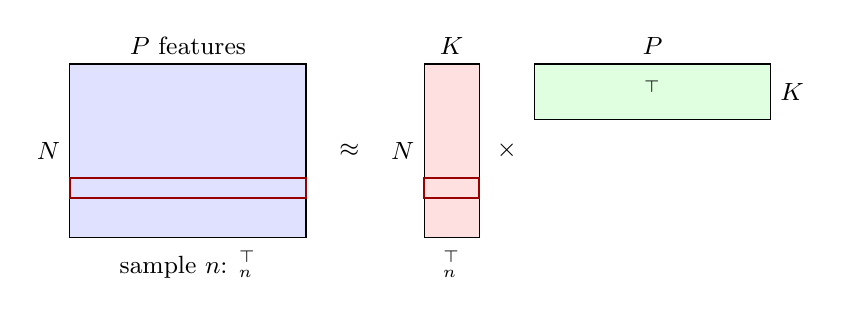
\begin{tikzpicture}[every node/.style={font=\small}]
    \draw[fill=blue!12] (0,0) rectangle (3.0,-2.2);
    \node at (1.5,-1.1) {$\mY$};
    \node[above] at (1.5,0) {$P$ features};
    \node[left] at (0,-1.1) {$N$};
    \node at (3.55,-1.1) {$\approx$};
    \draw[fill=red!12] (4.5,0) rectangle (5.2,-2.2);
    \node at (4.85,-1.1) {$\mX$};
    \node[above] at (4.85,0) {$K$};
    \node[left] at (4.5,-1.1) {$N$};
    \node at (5.55,-1.1) {$\times$};
    \draw[fill=green!12] (5.9,0) rectangle (8.9,-0.7);
    \node at (7.4,-0.35) {$\mW^\top$};
    \node[above] at (7.4,0) {$P$};
    \node[right] at (8.9,-0.35) {$K$};
    \draw[thick, red!60!black] (0,-1.45) rectangle (3.0,-1.7);
    \draw[thick, red!60!black] (4.5,-1.45) rectangle (5.2,-1.7);
    \node[below, align=center] at (1.5,-2.25) {sample $n$: $\vy_n^\top$};
    \node[below, align=center] at (4.85,-2.25) {$\vx_n^\top$};
  \end{tikzpicture}
  \caption{A matrix factorization approximates an $N\times P$ data matrix $\mY$ by the product of an $N\times K$ factor matrix $\mX$ and the transpose of a $P\times K$ loading matrix $\mW$. Row $n$ of $\mY$ is approximated by $\vx_n^\top\mW^\top$, a weighted sum of the $K$ columns of $\mW$.}
  \label{fig:mf_shapes}
\end{figure}

Many models fit this template. They differ in the assumptions they place on $\mX$, $\mW$ and the residual $\mY-\mX\mW^\top$:
\begin{itemize}
  \item principal components analysis (PCA), the classical method, and its probabilistic version, probabilistic PCA;
  \item factor analysis, which allows each feature its own noise variance;
  \item independent components analysis (ICA), which uses a heavy-tailed (sparse) distribution for the factors;
  \item non-negative matrix factorization (NMF), which constrains $\mX$ and $\mW$ to be non-negative;
  \item latent Dirichlet allocation~\citep{blei2003}, a model for count data that was the standard way to categorize documents into topics in natural language processing, and whose genetics analogue is the admixture model of population ancestry~\citep{pritchard2000};
  \item autoencoders, neural networks whose linear version is equivalent to PCA.
\end{itemize}

These models have many uses. They became widely known in machine learning through recommender systems. In the Netflix Prize competition, launched in 2006, Netflix released anonymized ratings of movies by its users and offered a million dollars for the best prediction of held-out ratings. Here $\mY$ is a users-by-movies matrix with most entries missing, and matrix factorization models were among the strongest single methods~\citep{koren2009}, although the winning entries averaged the predictions of many different models. In genomics matrix factorization is used for:
\begin{itemize}
  \item \emph{denoising} and \emph{imputation}: the low-rank reconstruction $\mX\mW^\top$ is less noisy than $\mY$ and provides values for missing entries;
  \item \emph{dimensionality reduction}: downstream analyses such as clustering can work with the $K$-dimensional $\vx_n$ instead of the $P$-dimensional $\vy_n$;
  \item \emph{visualization}: with $K=2$ the factors can be plotted;
  \item \emph{removing hidden confounders}: technical variation, such as batch, processing date or who ran the experiment, often affects many genes at once, so it is captured by a few factors that can be regressed out. We return to this use when we discuss expression quantitative trait loci in Chapter 12.
\end{itemize}

%======================================================================
\section{Factor analysis}
\label{sec:fa}
%======================================================================

\subsection{The model}

Factor analysis originated in psychology, in models of how latent kinds of intelligence affect performance on different tests~\citep{spearman1904}. Suppose $y_{pn}$ is student $n$'s score on question $p$, $x_{kn}$ is the student's ability of ``type'' $k$ (verbal or spatial reasoning, say), and $w_{pk}$ says how much question $p$ depends on ability $k$. The genomic analogue is that $y_{pn}$ is the expression of gene $p$ in cell or sample $n$, $x_{kn}$ is the activity of pathway or program $k$ in that sample, and $w_{pk}$ says how strongly gene $p$ responds to pathway $k$.

The factor analysis model for one data point is
\begin{equation}
  \vy_n = \mW\vx_n + \veps_n, \qquad [P\times 1]=[P\times K][K\times 1]+[P\times 1],
  \label{eq:fa}
\end{equation}
with
\begin{equation}
  \vx_n\sim\Normal(\vzero,\mI_K), \qquad \veps_n\sim\Normal(\vzero,\mPsi),
  \label{eq:fa_priors}
\end{equation}
independently for $n=1,\dots,N$. Here $\vy_n\in\R^P$ is observed, $\vx_n\in\R^K$ is latent, $\mW\in\R^{P\times K}$ is a parameter, and $\mPsi\in\R^{P\times P}$ is the noise covariance, which is diagonal, $\mPsi=\diag(\psi_1,\dots,\psi_P)$. Element-wise,
\begin{equation}
  y_{pn}=\sum_{k=1}^K w_{pk}x_{kn}+\epsilon_{pn}, \qquad \epsilon_{pn}\sim\Normal(0,\psi_p).
\end{equation}
There is no intercept: we assume the data have been \emph{centered}, so each column of $\mY$ has mean zero. The prior on $\vx_n$ has identity covariance without loss of generality. A factor with variance $s^2$ and loading column $\vw_k$ gives the same distribution of $\vy_n$ as a factor with unit variance and loading column $s\vw_k$, so any variance can be absorbed into $\mW$.

Because $\mPsi$ is diagonal, the features are independent given $\vx_n$. All the correlation between features is explained by the shared factors, while $\psi_p$ captures variation specific to feature $p$, such as measurement noise for that gene.

\subsection{Factor analysis models a covariance matrix}

The latent variable can be integrated out. Given $\vx_n$, $\vy_n\mid\vx_n\sim\Normal(\mW\vx_n,\mPsi)$, and the marginal distribution is
\begin{equation}
  p(\vy_n) = \int \Normal(\vy_n\mid\mW\vx_n,\mPsi)\,\Normal(\vx_n\mid\vzero,\mI)\,d\vx_n.
\end{equation}
Rather than computing the integral directly, note that $\vy_n$ is a linear function of the jointly Gaussian vector $(\vx_n,\veps_n)$, so $\vy_n$ is Gaussian and we only need its mean and covariance. The mean is $\E[\vy_n]=\mW\E[\vx_n]+\E[\veps_n]=\vzero$. Since $\vx_n$ and $\veps_n$ are independent with zero mean, the covariance is
\begin{equation}
  \E[\vy_n\vy_n^\top] = \mW\E[\vx_n\vx_n^\top]\mW^\top + \E[\veps_n\veps_n^\top] = \mW\mW^\top+\mPsi,
\end{equation}
so
\begin{equation}
  \vy_n\sim\Normal(\vzero,\mC), \qquad \mC=\mW\mW^\top+\mPsi, \qquad [P\times P]=[P\times K][K\times P]+[P\times P].
  \label{eq:fa_marginal}
\end{equation}
Factor analysis is therefore a model of the $P\times P$ covariance matrix of the data, with a low-rank-plus-diagonal structure. A full covariance matrix has $P(P+1)/2$ free parameters, while $\mC$ has $PK+P$, which for $P=10{,}000$ genes and $K=10$ factors is about $10^5$ rather than $5\times10^7$. Many of the matrix factorization models in this chapter can be understood in the same way, as learning a structured covariance for the data.

Equation~\eqref{eq:fa_marginal} also shows that $\mW$ is not identifiable. For any orthogonal $K\times K$ matrix $\mR$ ($\mR\mR^\top=\mI$), the loadings $\mW\mR$ give $(\mW\mR)(\mW\mR)^\top=\mW\mW^\top$ and hence the same likelihood. Equivalently, replacing $\vx_n$ by $\mR^\top\vx_n$ leaves its $\Normal(\vzero,\mI)$ distribution unchanged. The model determines the $K$-dimensional subspace spanned by the columns of $\mW$, but not a particular basis for it. Interpretable bases are chosen afterwards (for example by varimax rotation), or by changing the model so that rotations no longer leave the likelihood unchanged, as ICA and NMF do.

\subsection{Connection to mixture models}

The Gaussian mixture model of Chapter 5 can be written in the same form. With cluster means $\vmu_1,\dots,\vmu_K\in\R^P$ collected as the columns of $\mM\in\R^{P\times K}$ and a one-hot cluster indicator $\vz_n\in\{0,1\}^K$,
\begin{equation}
  \vy_n = \mM\vz_n+\veps_n, \qquad \veps_n\sim\Normal(\vzero,\sigma^2\mI).
\end{equation}
After EM, the posterior expectation of the mean of $\vy_n$ is $\sum_k\vmu_k\gamma_{nk}$, where $\gamma_{nk}=p(z_{nk}=1\mid\vy_n)$ is the responsibility of cluster $k$ for point $n$. This is a matrix factorization with $\mW=\mM$ and $\vx_n=\vgamma_n$. The difference lies in the constraint on the factors: in a mixture model $\vx_n$ is one-hot (or, for the soft assignments, a probability vector), so each point is described by one prototype, while in factor analysis $\vx_n$ is any real vector, so each point is a combination of several factors.

%======================================================================
\section{Fitting factor analysis}
\label{sec:fa_fit}
%======================================================================

\subsection{Direct maximization of the marginal likelihood}

Since the marginal distribution~\eqref{eq:fa_marginal} does not involve $\vx_n$, we can estimate $\mW$ and $\mPsi$ by maximum likelihood without dealing with the latent variables. Writing $\mC=\mW\mW^\top+\mPsi$, the log likelihood of the $N$ independent data points is
\begin{align}
  \log L(\mW,\mPsi) &= \sum_{n=1}^N\log\Normal(\vy_n\mid\vzero,\mC) \nonumber\\
  &= -\frac{NP}{2}\log 2\pi-\frac{N}{2}\log|\mC|-\frac12\sum_{n=1}^N\vy_n^\top\mC^{-1}\vy_n.
  \label{eq:fa_loglik}
\end{align}
The first term is constant. The second is the normalizing term of the Gaussian and penalizes a large covariance; the third measures the fit to the data. Using $\vy_n^\top\mC^{-1}\vy_n=\tr(\mC^{-1}\vy_n\vy_n^\top)$ and defining the sample covariance
\begin{equation}
  \mS=\frac1N\sum_{n=1}^N\vy_n\vy_n^\top=\frac1N\mY^\top\mY \in\R^{P\times P},
  \label{eq:S}
\end{equation}
the log likelihood depends on the data only through $\mS$,
\begin{equation}
  \log L = -\frac N2\left[P\log2\pi+\log|\mC|+\tr(\mC^{-1}\mS)\right].
  \label{eq:fa_loglik_S}
\end{equation}
There is no closed-form maximizer for general diagonal $\mPsi$. One option is to write~\eqref{eq:fa_loglik} in an automatic differentiation framework (PyTorch, JAX) and minimize $-\log L$ by gradient descent, parameterizing $\psi_p=e^{\theta_p}$ to keep the variances positive. Computing $\mC^{-1}$ and $|\mC|$ costs $O(P^3)$ when done naively, but the Woodbury identity and the matrix determinant lemma reduce this to $O(PK^2)$:
\begin{equation}
  \mC^{-1}=\mPsi^{-1}-\mPsi^{-1}\mW(\mI+\mW^\top\mPsi^{-1}\mW)^{-1}\mW^\top\mPsi^{-1}, \qquad
  |\mC| = |\mPsi|\,|\mI+\mW^\top\mPsi^{-1}\mW|,
\end{equation}
which involve only the diagonal $\mPsi$ and $K\times K$ inverses.

\subsection{Expectation maximization}

The alternative is the EM algorithm of Chapter 5, treating $\vx_n$ as the latent variable~\citep{rubin1982,ghahramani1996}. The E-step computes $q(\vx_n)=p(\vx_n\mid\vy_n,\mW,\mPsi)$ at the current parameters; the M-step maximizes the expected complete-data log likelihood over $\mW$ and $\mPsi$.

\paragraph{E-step.} By Bayes' rule $p(\vx_n\mid\vy_n)\propto\Normal(\vy_n\mid\mW\vx_n,\mPsi)\,\Normal(\vx_n\mid\vzero,\mI)$. Collecting the terms of the log that depend on $\vx_n$,
\begin{align}
  \log p(\vx_n\mid\vy_n) &= -\frac12(\vy_n-\mW\vx_n)^\top\mPsi^{-1}(\vy_n-\mW\vx_n)-\frac12\vx_n^\top\vx_n+\text{const} \nonumber\\
  &= -\frac12\vx_n^\top\left(\mI+\mW^\top\mPsi^{-1}\mW\right)\vx_n+\vx_n^\top\mW^\top\mPsi^{-1}\vy_n+\text{const}.
\end{align}
This is quadratic in $\vx_n$, so the posterior is Gaussian. Matching it to $-\frac12(\vx_n-\vm_n)^\top\mSigma^{-1}(\vx_n-\vm_n)$, which expands to $-\frac12\vx_n^\top\mSigma^{-1}\vx_n+\vx_n^\top\mSigma^{-1}\vm_n+\text{const}$, gives
\begin{equation}
  \vx_n\mid\vy_n\sim\Normal(\vm_n,\mSigma), \qquad \mSigma=\left(\mI_K+\mW^\top\mPsi^{-1}\mW\right)^{-1}, \qquad \vm_n=\mSigma\mW^\top\mPsi^{-1}\vy_n.
  \label{eq:fa_estep}
\end{equation}
The posterior covariance $\mSigma$ ($K\times K$) is the same for every data point, and the posterior mean $\vm_n\in\R^K$ is a linear function of $\vy_n$. The M-step needs the expected sufficient statistics
\begin{equation}
  \E[\vx_n]=\vm_n, \qquad \E[\vx_n\vx_n^\top]=\mSigma+\vm_n\vm_n^\top.
\end{equation}

\paragraph{M-step.} The expected complete-data log likelihood, dropping the prior on $\vx_n$, which does not depend on the parameters, is
\begin{equation}
  Q(\mW,\mPsi) = -\frac N2\log|\mPsi|-\frac12\sum_{n=1}^N\E\left[(\vy_n-\mW\vx_n)^\top\mPsi^{-1}(\vy_n-\mW\vx_n)\right]+\text{const}.
\end{equation}
Expanding the quadratic form, $\E[(\vy_n-\mW\vx_n)^\top\mPsi^{-1}(\vy_n-\mW\vx_n)]=\vy_n^\top\mPsi^{-1}\vy_n-2\vy_n^\top\mPsi^{-1}\mW\vm_n+\tr(\mW^\top\mPsi^{-1}\mW\,\E[\vx_n\vx_n^\top])$. Setting the derivative with respect to $\mW$ to zero,
\begin{equation}
  \frac{\partial Q}{\partial\mW}=\mPsi^{-1}\sum_n\left(\vy_n\vm_n^\top-\mW\E[\vx_n\vx_n^\top]\right)=\vzero
  \quad\Rightarrow\quad
  \mW^{\text{new}}=\left(\sum_n\vy_n\vm_n^\top\right)\left(\sum_n\E[\vx_n\vx_n^\top]\right)^{-1}.
  \label{eq:fa_mstep_W}
\end{equation}
This is the least-squares regression of $\vy_n$ on $\vx_n$ with the unknown $\vx_n$ replaced by its expected sufficient statistics. For the diagonal of $\mPsi$, the terms involving $\psi_p$ are $-\frac N2\log\psi_p-\frac1{2\psi_p}\sum_n\E[(y_{pn}-\vw_p^\top\vx_n)^2]$, where $\vw_p^\top$ is row $p$ of $\mW$. Setting the derivative to zero gives $\psi_p=\frac1N\sum_n\E[(y_{pn}-\vw_p^\top\vx_n)^2]$, the expected squared residual of feature $p$. Expanding the square and using~\eqref{eq:fa_mstep_W}, which implies $\vw_p^\top\sum_n\E[\vx_n\vx_n^\top]\vw_p=\vw_p^\top\sum_n\vm_ny_{pn}$, this simplifies to
\begin{equation}
  \psi_p^{\text{new}}=\frac1N\sum_{n=1}^N\left(y_{pn}^2-\vw_p^{\text{new}\top}\vm_ny_{pn}\right),
  \qquad\text{or}\qquad
  \mPsi^{\text{new}}=\diag\left(\mS-\mW^{\text{new}}\frac1N\sum_n\vm_n\vy_n^\top\right).
\end{equation}
Each EM iteration costs $O(NPK)$ and, as shown in Chapter 5, never decreases the log likelihood~\eqref{eq:fa_loglik}. A practical advantage of EM, and of the probabilistic formulation in general, is that missing entries of $\mY$ are handled by dropping them from the sums.

%======================================================================
\section{Multi-omics factor analysis}
\label{sec:mofa}
%======================================================================

\subsection{The model}

Patient cohorts are increasingly profiled with several assays: RNA-seq for gene expression, ATAC-seq for chromatin accessibility, DNA methylation arrays, somatic mutation calls, proteomics. \emph{Multi-omics factor analysis} (MOFA) extends factor analysis to model all of these matrices jointly~\citep{argelaguet2018}; MOFA+ adapts it to single-cell data~\citep{argelaguet2020}. There are $M$ data matrices (``views'') $\mY^{(m)}\in\R^{N\times D_m}$, $m=1,\dots,M$, measured on the same $N$ samples, where $D_m$ is the number of features in view $m$: genes for RNA-seq, accessible regions (peaks) for ATAC-seq, CpG sites for methylation. MOFA decomposes each as
\begin{equation}
  \mY^{(m)} = \mX\mW^{(m)\top}+\mE^{(m)}, \qquad m=1,\dots,M,
  \label{eq:mofa}
\end{equation}
with a factor matrix $\mX\in\R^{N\times K}$ shared by all views and a view-specific loading matrix $\mW^{(m)}\in\R^{D_m\times K}$ (Figure~\ref{fig:mofa_schematic}). The factors are shared because they represent the underlying biological state of each sample, which all assays reflect. The loadings differ because each view has its own features. Not every sample needs to be measured in every view: missing samples or entries are left out of the likelihood, and the shared $\vx_n$ is inferred from whichever views are available.

\begin{figure}[tbp]
  \centering
  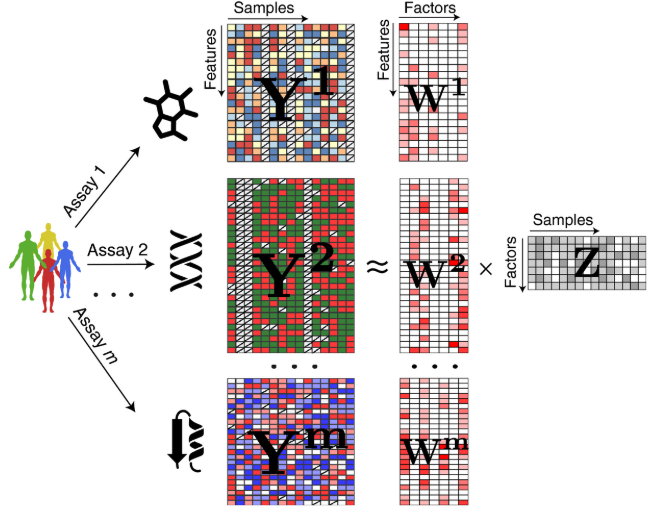
\includegraphics[width=0.75\linewidth]{slides/mofa_schematic.png}
  \caption{Multi-omics factor analysis. Several assays on the same samples give data matrices $\mY^1,\dots,\mY^m$ (drawn as features by samples, the transpose of our convention), each with its own loading matrix $\mW^m$ and a shared factor matrix $\mathbf{Z}$ (our $\mX$). Hatched entries are missing. Reproduced from \citet{argelaguet2018}.}
  \label{fig:mofa_schematic}
\end{figure}

The priors are
\begin{align}
  x_{nk}&\sim\Normal(0,1), \\
  \epsilon^{(m)}_{nd}&\sim\Normal\left(0,1/\tau^{(m)}_d\right), & \tau^{(m)}_d&\sim\Gam(a_0^\tau,b_0^\tau), \\
  w^{(m)}_{dk}&\sim\Normal\left(0,1/\alpha^{(m)}_k\right), & \alpha^{(m)}_k&\sim\Gam(a_0^\alpha,b_0^\alpha).
  \label{eq:mofa_ard}
\end{align}
The prior on the factors is the same as in factor analysis. The noise precision (inverse variance) $\tau^{(m)}_d$ is specific to each feature $d$ of each view, so as in factor analysis some genes can be noisier than others. MOFA also supports non-Gaussian likelihoods for binary data such as mutations and for counts. The new ingredient is the prior on the loadings.

\subsection{Automatic relevance determination}

The prior variance of $w^{(m)}_{dk}$ is $1/\alpha^{(m)}_k$, shared by all features of view $m$ for factor $k$. The $\alpha$s are precisions, and they are learned, with a Gamma prior
\begin{equation}
  \Gam(\alpha\mid a,b)=\frac{b^a}{\Gamma(a)}\alpha^{a-1}e^{-b\alpha}, \qquad \alpha>0,
\end{equation}
which has mean $a/b$. The shape $a$ controls the form of the density (Figure~\ref{fig:gamma_ard}): for $a>1$ it is a unimodal bump on the positive axis, for $a=1$ it is exponential, and for $a<1$ it diverges at zero and has a long tail. MOFA sets $a_0^\alpha=b_0^\alpha=10^{-14}$, so the prior is close to $p(\alpha)\propto1/\alpha$: it is indifferent to the scale of $\alpha$ and allows both very small and very large values.

\begin{figure}[tbp]
  \centering
  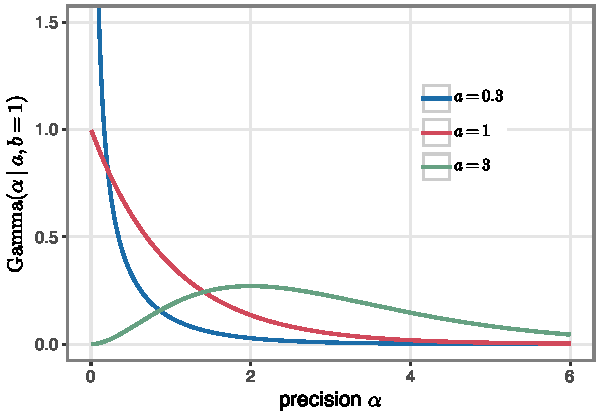
\includegraphics[width=0.5\linewidth]{gamma_ard.pdf}
  \caption{Gamma densities with rate $b=1$ and three shapes $a$. For $a<1$ most of the mass is near zero with a long tail to large values.}
  \label{fig:gamma_ard}
\end{figure}

The effect is to switch factors on and off per view. If $\alpha^{(m)}_k$ is large, the prior variance $1/\alpha^{(m)}_k$ is close to zero, and all loadings of factor $k$ on view $m$ are forced to zero: factor $k$ does not affect that assay. If $\alpha^{(m)}_k$ is small, the prior variance is large and the loadings are free to be large. Learning $\alpha$ from the data therefore determines which factors are relevant to which views, hence the name \emph{automatic relevance determination} (ARD)~\citep{mackay1994,neal1996,bishop1999bpca}. A factor can be active in one view only (for example capturing variation specific to the RNA-seq data), in all views, or in a subset, and the shared factors are often the most interesting. Applied across all factors of a single view, the same prior prunes factors that are not needed, which reduces the sensitivity to the choice of $K$. MOFA additionally places a spike-and-slab prior on each loading, $w^{(m)}_{dk}=\hat w^{(m)}_{dk}s^{(m)}_{dk}$ with $\hat w^{(m)}_{dk}$ following~\eqref{eq:mofa_ard} and $s^{(m)}_{dk}\in\{0,1\}$ Bernoulli, so that each factor affects only some features within an active view. The posterior over all the latent variables and parameters is approximated by variational Bayesian inference, which we cover in a later chapter.

The same factor analysis structure with ARD priors is used by PEER~\citep{stegle2010} to infer hidden confounders in gene expression, which we meet in Chapter 12.

\subsection{Application: chronic lymphocytic leukemia}

\citet{argelaguet2018} applied MOFA to a cohort of 200 patients with chronic lymphocytic leukemia (CLL) profiled with four views: somatic mutations (69 features), RNA-seq (5000 genes), DNA methylation (4248 CpG sites) and \emph{ex vivo} drug response of the patients' cancer cells (310 features, responses to a panel of drugs at several concentrations). Not all patients had every assay (Figure~\ref{fig:mofa_cll}A). The model found 10 factors. Panel B shows the variance explained ($R^2$) by each factor in each view, which reflects the relevance learned through $\alpha^{(m)}_k$: a factor switched off in a view explains no variance there. Factor 1 explains variation in methylation, mutations and drug response, and less in RNA; factor 3 is specific to drug response; factor 4 is specific to gene expression.

The loadings identify the factors (panel D). Factor 1 is driven by the mutation status of the immunoglobulin heavy-chain variable region (IGHV), the main clinical subtype of CLL, and factor 2 by trisomy 12, a gain of a third copy of chromosome 12. A scatter plot of the two factors (panel E) separates patients by these two genetic features. Other factors relate to gene sets (panel F), for example immune response and cellular stress pathways. The general point is that multi-omic data are high-dimensional in each view and heterogeneous across views, and a factor model with view-specific relevance finds a few axes of variation and identifies which are shared across data types.

\begin{figure}[tbp]
  \centering
  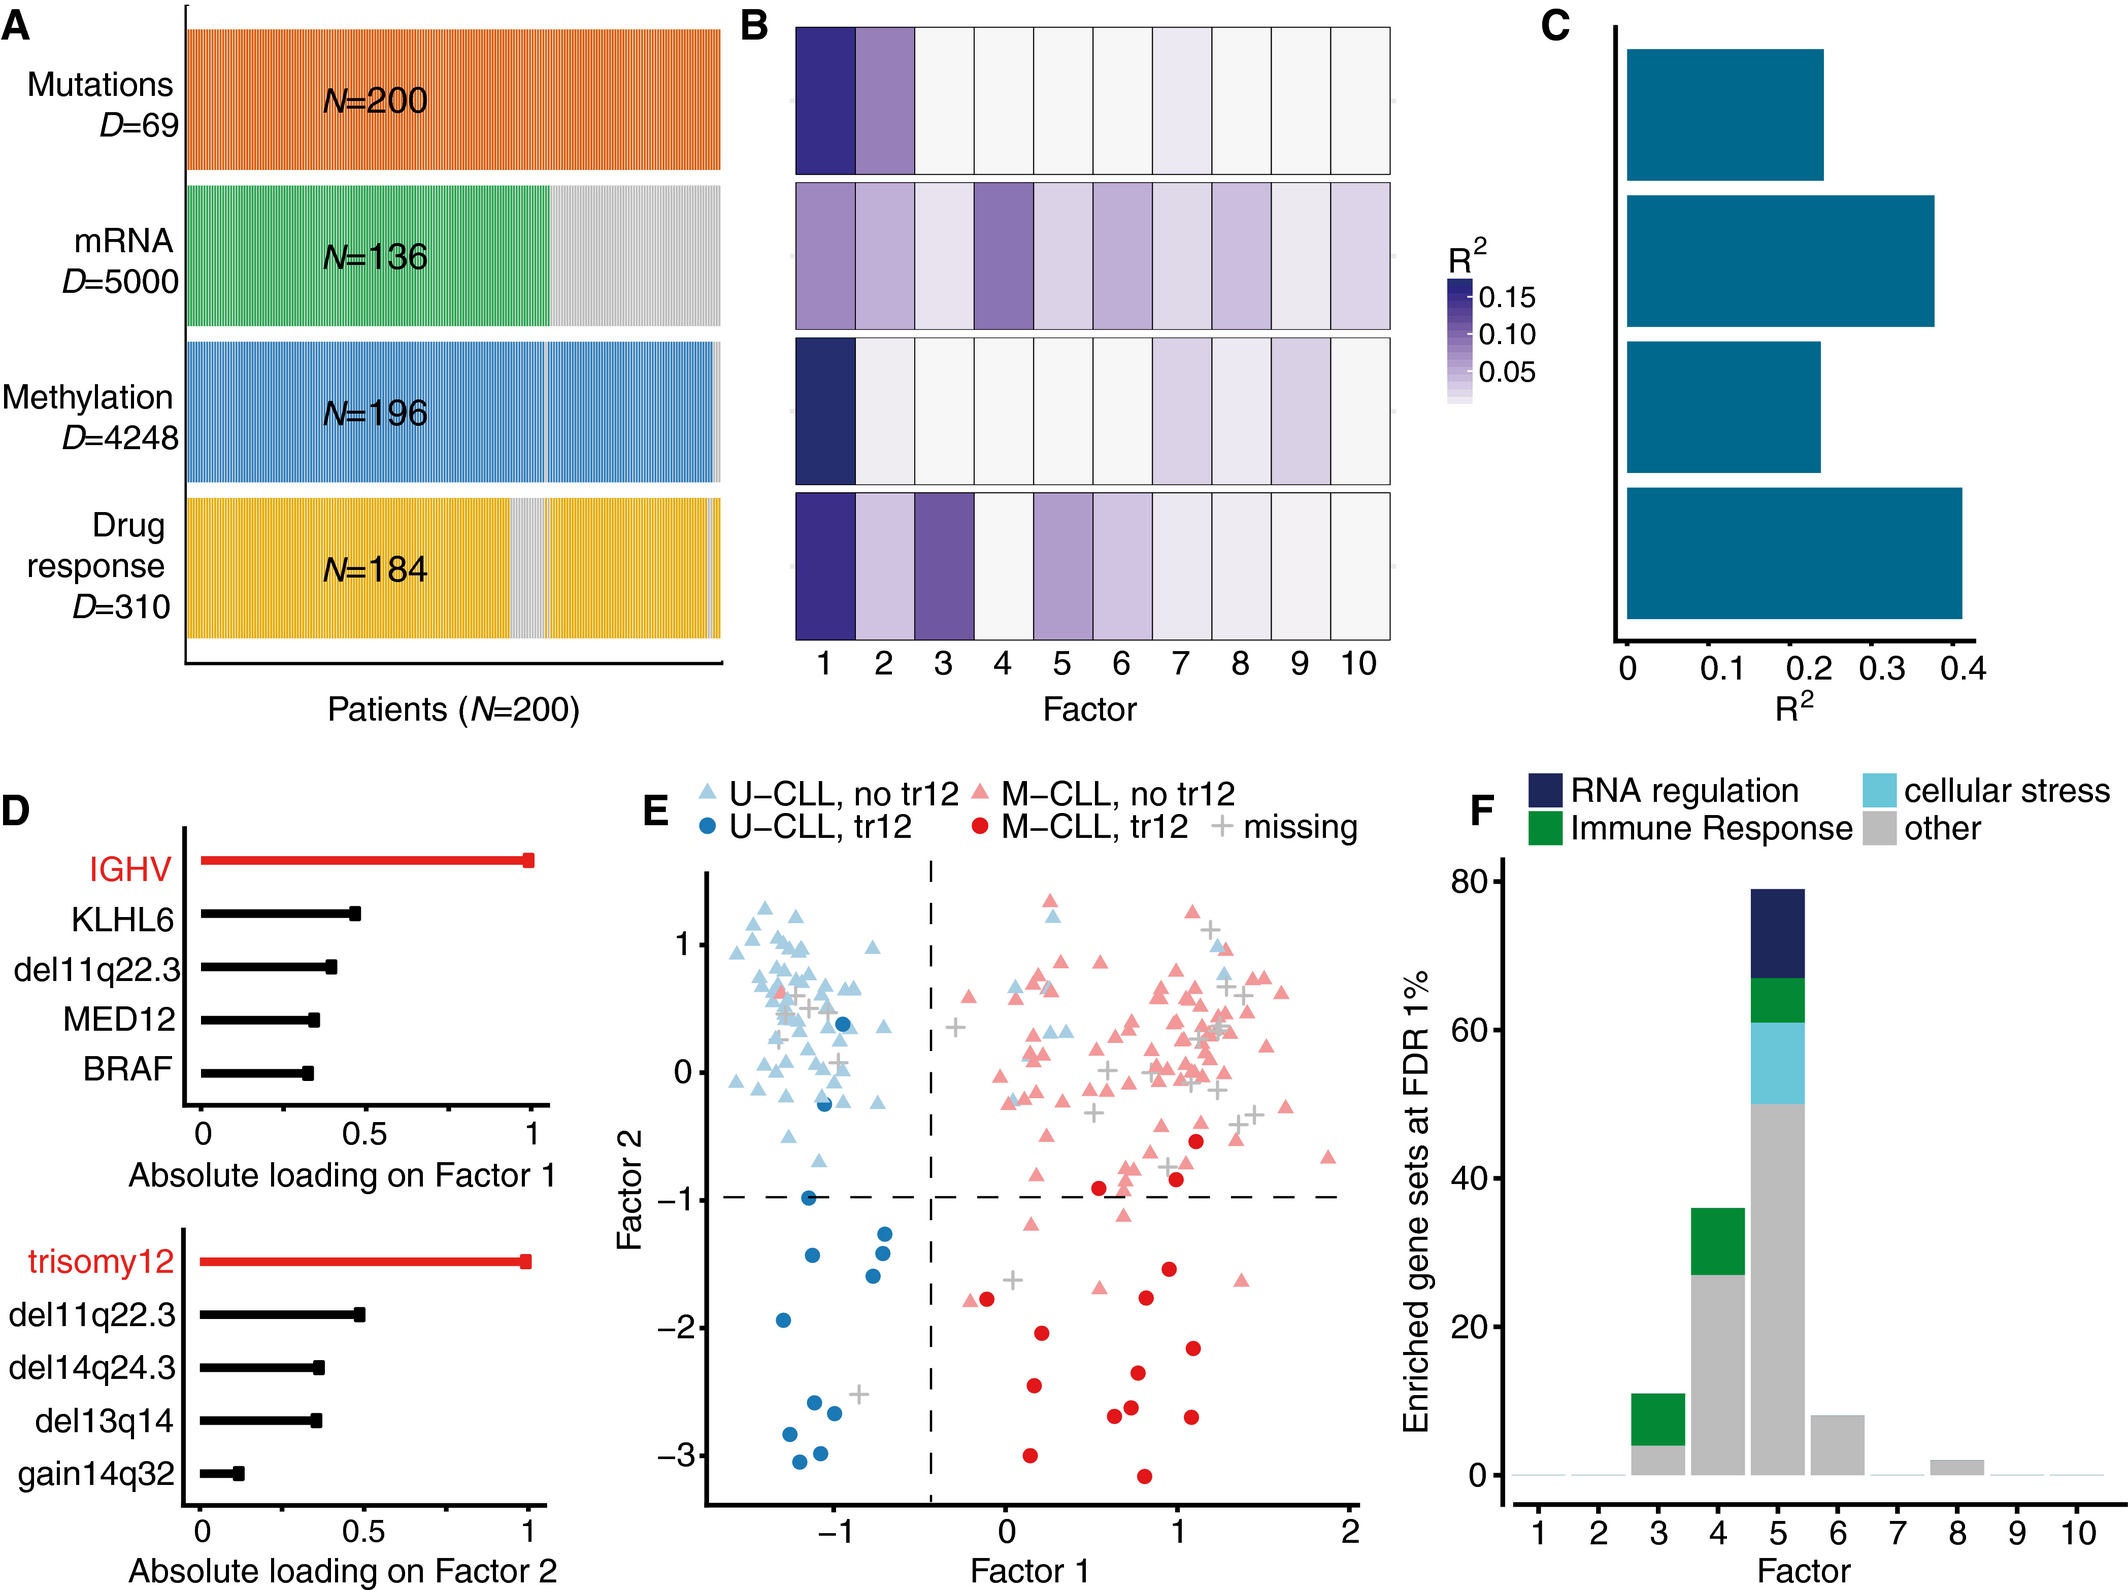
\includegraphics[width=0.95\linewidth]{slides/mofa_cll.png}
  \caption{MOFA applied to chronic lymphocytic leukemia. (A) Four views measured on 200 patients; grey marks missing samples. (B) Variance explained by each factor in each view. (C) Total variance explained per view. (D) Largest absolute loadings of factors 1 and 2 on the mutation view. (E) Patients plotted by factors 1 and 2, coloured by IGHV status (U, unmutated; M, mutated) and trisomy 12. (F) Number of gene sets enriched in the mRNA loadings of each factor. Reproduced from \citet{argelaguet2018}.}
  \label{fig:mofa_cll}
\end{figure}

%======================================================================
\section{Probabilistic principal components analysis}
\label{sec:ppca}
%======================================================================

\subsection{Spherical noise}

Probabilistic PCA~\citep{tipping1999} is factor analysis with one change: the noise covariance is \emph{spherical}, $\mPsi=\sigma^2\mI_P$, a single variance $\sigma^2$ shared by all features,
\begin{equation}
  \vy_n=\mW\vx_n+\veps_n, \qquad \vx_n\sim\Normal(\vzero,\mI_K), \qquad \veps_n\sim\Normal(\vzero,\sigma^2\mI_P),
  \label{eq:ppca}
\end{equation}
so that $\vy_n\sim\Normal(\vzero,\mC)$ with $\mC=\mW\mW^\top+\sigma^2\mI$. Factor analysis allows a separate noise level for each feature; probabilistic PCA assumes they are all equal. Which assumption is better depends on the data. If the features are on different scales or some are much noisier than others, the spherical assumption pushes probabilistic PCA to spend factors explaining the noise of individual features. Figure~\ref{fig:fa_vs_ppca} shows an example with one factor that loads on five features and a sixth feature with large independent noise. Factor analysis recovers the loadings and puts the sixth feature's variance into $\psi_6$; probabilistic PCA with $K=1$ points its single component at the noisy feature, because that is the direction of largest variance. For this reason expression data are usually log-transformed and often standardized before PCA. The advantage of the spherical model is computational: its maximum likelihood estimate has a closed form.

\begin{figure}[tbp]
  \centering
  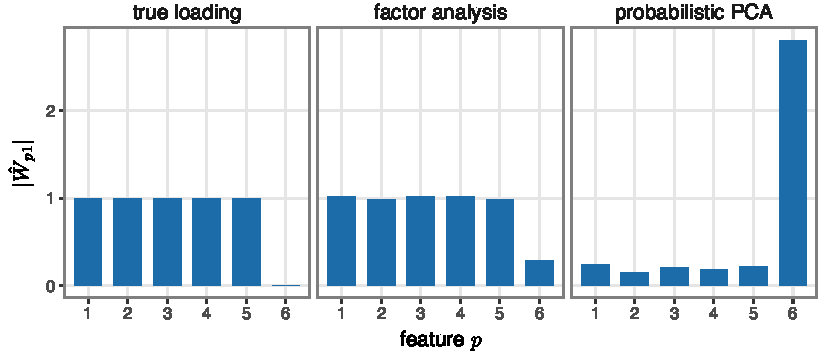
\includegraphics[width=0.85\linewidth]{fa_vs_ppca.pdf}
  \caption{Factor analysis and probabilistic PCA with $K=1$ fitted to $N=500$ simulated points. The true factor loads on features 1--5 (noise variance 0.3 each); feature 6 has no loading and noise variance 9. Factor analysis recovers the loadings; probabilistic PCA puts its component on the noisy feature.}
  \label{fig:fa_vs_ppca}
\end{figure}

\subsection{Maximum likelihood by eigendecomposition}

The log likelihood is~\eqref{eq:fa_loglik_S} with $\mC=\mW\mW^\top+\sigma^2\mI$. The sample covariance $\mS=\frac1N\mY^\top\mY$ is symmetric and positive semi-definite (positive definite if $N>P$ and $\mY$ has full column rank), so it has an eigendecomposition
\begin{equation}
  \mS=\mU\mLambda\mU^\top, \qquad \mU^\top\mU=\mI_P, \qquad \mLambda=\diag(\lambda_1,\dots,\lambda_P),
  \label{eq:eig}
\end{equation}
where $\mU\in\R^{P\times P}$ is orthogonal, its columns $\vu_k$ are the eigenvectors, $\mS\vu_k=\lambda_k\vu_k$, and the eigenvalues are ordered, $\lambda_1\geq\lambda_2\geq\dots\geq\lambda_P\geq0$. Write $\mU_K=\mU[:,1{:}K]$ for the first $K$ columns and $\mLambda_K=\mLambda[1{:}K,1{:}K]$ for the $K$ largest eigenvalues. \citet{tipping1999} showed that the maximum likelihood estimates are
\begin{equation}
  \hat\mW=\mU_K\left(\mLambda_K-\hat\sigma^2\mI_K\right)^{1/2}\mR, \qquad \hat\sigma^2=\frac1{P-K}\sum_{k=K+1}^P\lambda_k,
  \label{eq:ppca_ml}
\end{equation}
where $\mR$ is any $K\times K$ orthogonal matrix, reflecting the rotational non-identifiability, and is usually taken to be $\mI$. The directions of $\hat\mW$ are the $K$ leading eigenvectors of $\mS$. The diagonal matrix $(\mLambda_K-\hat\sigma^2\mI)^{1/2}$ rescales each column $\vu_k$ by $\sqrt{\lambda_k-\hat\sigma^2}$ without changing its direction. The noise variance is the average of the $P-K$ discarded eigenvalues: variance in the directions we do not model as signal is attributed to noise.

To see where~\eqref{eq:ppca_ml} comes from, differentiate~\eqref{eq:fa_loglik_S} with respect to $\mW$. Using $\partial\log|\mC|/\partial\mW=2\mC^{-1}\mW$ and $\partial\tr(\mC^{-1}\mS)/\partial\mW=-2\mC^{-1}\mS\mC^{-1}\mW$ for symmetric $\mC$ and $\mS$, the stationary points satisfy
\begin{equation}
  \mS\mC^{-1}\mW=\mW.
\end{equation}
The push-through identity $(\mW\mW^\top+\sigma^2\mI_P)^{-1}\mW=\mW(\mW^\top\mW+\sigma^2\mI_K)^{-1}$ turns this into $\mS\mW=\mW(\sigma^2\mI+\mW^\top\mW)$. Write the singular value decomposition $\mW=\mL\mD\mR^\top$, with $\mL\in\R^{P\times K}$ having orthonormal columns $\boldsymbol{\ell}_k$, $\mD=\diag(d_1,\dots,d_K)$ and $\mR$ orthogonal. Then $\mW^\top\mW=\mR\mD^2\mR^\top$, and the stationarity condition becomes $\mS\mL\mD\mR^\top=\mL\mD(\sigma^2\mI+\mD^2)\mR^\top$, that is,
\begin{equation}
  \mS\boldsymbol{\ell}_k=(\sigma^2+d_k^2)\,\boldsymbol{\ell}_k \qquad\text{for each }k\text{ with }d_k\neq0.
\end{equation}
Each column direction of $\mW$ is an eigenvector of $\mS$, with eigenvalue $\lambda=\sigma^2+d_k^2$, so $d_k=\sqrt{\lambda-\sigma^2}$. Any $K$ eigenvectors give a stationary point, and \citet{tipping1999} show that the maximum takes those with the $K$ largest eigenvalues; the others are saddle points. Substituting back and maximizing over $\sigma^2$ gives the average of the remaining eigenvalues.

This is unusual: a latent variable model with a likelihood that is not convex in $\mW$ can be fitted exactly, with one call to a standard eigendecomposition routine. The probabilistic formulation also gives a posterior over the factors, the special case of~\eqref{eq:fa_estep} with $\mPsi=\sigma^2\mI$,
\begin{equation}
  \vx_n\mid\vy_n\sim\Normal\left(\mM^{-1}\mW^\top\vy_n,\ \sigma^2\mM^{-1}\right), \qquad \mM=\mW^\top\mW+\sigma^2\mI_K\in\R^{K\times K},
  \label{eq:ppca_post}
\end{equation}
handles missing data through EM, and gives a likelihood with which to compare models.

\subsection{Choosing the number of components}

The eigenvalue $\lambda_k$ is the variance of the data along $\vu_k$, and the \emph{proportion of variance explained} by component $k$ is
\begin{equation}
  \text{PVE}_k=\frac{\lambda_k}{\sum_{k'=1}^P\lambda_{k'}}.
\end{equation}
A plot of the ordered eigenvalues (a \emph{scree plot}, Figure~\ref{fig:eigen}a) typically shows a few large ``signal'' eigenvalues followed by a long tail of small ``noise'' eigenvalues, and a common heuristic is to choose $K$ at the elbow. Two more principled approaches follow from the probabilistic view.

First, the Bayesian treatment of probabilistic PCA allows the marginal likelihood $p(\mY\mid K)$, with $\mW$ integrated out, to be approximated for each $K$~\citep{minka2000}. Choosing the $K$ with the largest approximate marginal likelihood decides how many eigenvectors to treat as signal and how many as noise. Minka's method is implemented in scikit-learn (\texttt{PCA(n\_components="mle")}).

Second, random matrix theory says what the noise eigenvalues should look like. Even if the true covariance is $\sigma^2\mI$, the eigenvalues of the sample covariance are spread out. If the entries of $\mY$ are independent with variance $\sigma^2$, and $N,P\to\infty$ with $P/N\to\gamma\in(0,1]$, the distribution of the eigenvalues of $\mS$ converges to the Marchenko-Pastur law~\citep{marchenko1967}, with density
\begin{equation}
  p(\lambda)=\frac{\sqrt{(\lambda_+-\lambda)(\lambda-\lambda_-)}}{2\pi\sigma^2\gamma\lambda}, \qquad \lambda_-\leq\lambda\leq\lambda_+, \qquad \lambda_\pm=\sigma^2(1\pm\sqrt\gamma)^2.
\end{equation}
Eigenvalues above the upper edge $\lambda_+$ are evidence of signal (Figure~\ref{fig:eigen}). With $N=1000$ samples and $P=200$ features, pure noise of unit variance already produces sample eigenvalues ranging from $0.31$ to $2.09$. Conversely, a factor whose contribution to the variance, $\|\vw_k\|^2$, is below $\sigma^2\sqrt\gamma$ produces no eigenvalue outside the noise bulk and cannot be detected by PCA at all~\citep{baik2005}.

\begin{figure}[tbp]
  \centering
  \begin{subfigure}[b]{0.49\linewidth}
    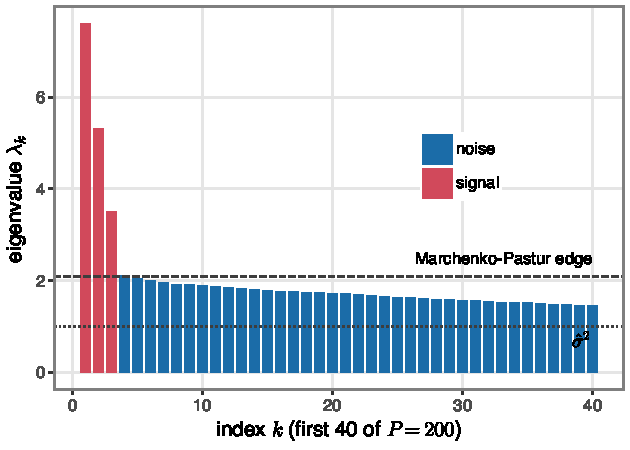
\includegraphics[width=\linewidth]{eigen_scree.pdf}
    \caption{}
  \end{subfigure}\hfill
  \begin{subfigure}[b]{0.49\linewidth}
    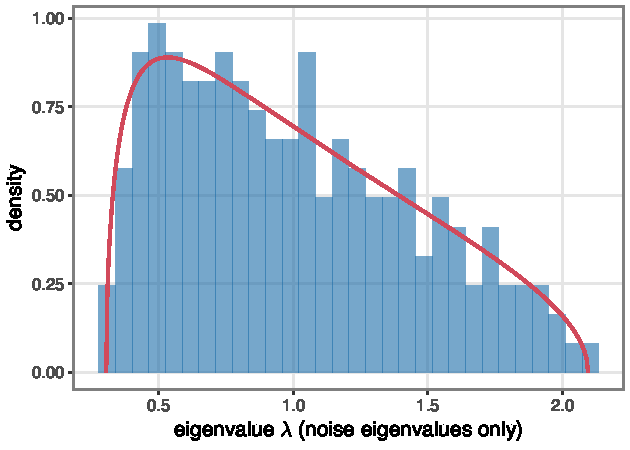
\includegraphics[width=\linewidth]{eigen_mp.pdf}
    \caption{}
  \end{subfigure}
  \caption{Eigenvalues of the sample covariance of simulated data with $N=1000$, $P=200$, $K=3$ factors and noise variance $\sigma^2=1$. (a) The three signal eigenvalues stand above the Marchenko-Pastur upper edge $\lambda_+=(1+\sqrt{0.2})^2\approx2.09$ (dashed); the probabilistic PCA estimate $\hat\sigma^2$, the mean of the remaining eigenvalues, is $0.997$ (dotted). (b) The $197$ noise eigenvalues follow the Marchenko-Pastur density (curve).}
  \label{fig:eigen}
\end{figure}

%======================================================================
\section{Principal components analysis}
\label{sec:pca}
%======================================================================

\subsection{PCA as a limit of probabilistic PCA}

Historically PCA came first~\citep{pearson1901,hotelling1933} and probabilistic PCA was introduced to give it a probabilistic interpretation. Going in the other direction, classical PCA is the limit of probabilistic PCA in which all components are kept, $K\to P$, so that no variance is left for the noise, $\hat\sigma^2\to0$. Then~\eqref{eq:ppca_ml} becomes
\begin{equation}
  \hat\mW=\mU\mLambda^{1/2},
\end{equation}
and $\hat\mW\hat\mW^\top=\mU\mLambda\mU^\top=\mS$ reproduces the sample covariance exactly. As $\sigma^2\to0$ the posterior mean~\eqref{eq:ppca_post} tends to $(\mW^\top\mW)^{-1}\mW^\top\vy_n$, the coordinates of the orthogonal projection of $\vy_n$ onto the column space of $\mW$. In practice one keeps the first $K$ components. The \emph{principal component scores} are the projections $\mY\mU_K\in\R^{N\times K}$, and the rank-$K$ reconstruction $\mY\mU_K\mU_K^\top$ is the best rank-$K$ approximation of $\mY$ in squared error (the Eckart-Young theorem).

\subsection{PCA as the directions of maximal variance}

The classical definition of PCA is that it finds the orthogonal directions along which the data vary most (Figure~\ref{fig:pca_2d}). The variance of the centered data projected onto a unit vector $\vu\in\R^P$ is $\frac1N\sum_n(\vu^\top\vy_n)^2=\vu^\top\mS\vu$. Maximizing this subject to $\vu^\top\vu=1$ with a Lagrange multiplier $\lambda$,
\begin{equation}
  \frac{\partial}{\partial\vu}\left[\vu^\top\mS\vu-\lambda(\vu^\top\vu-1)\right]=2\mS\vu-2\lambda\vu=\vzero
  \quad\Rightarrow\quad \mS\vu=\lambda\vu,
\end{equation}
so $\vu$ is an eigenvector of $\mS$ and the projected variance is $\vu^\top\mS\vu=\lambda$. The maximum is the first eigenvector $\vu_1$, with variance $\lambda_1$. The second principal component maximizes the variance among directions orthogonal to $\vu_1$, which is equivalent to removing the variation along $\vu_1$ and repeating, and gives $\vu_2$; and so on. Eigenvectors of a symmetric matrix are orthogonal, $\vu_i^\top\vu_j=0$ for $i\neq j$.

\begin{figure}[tbp]
  \centering
  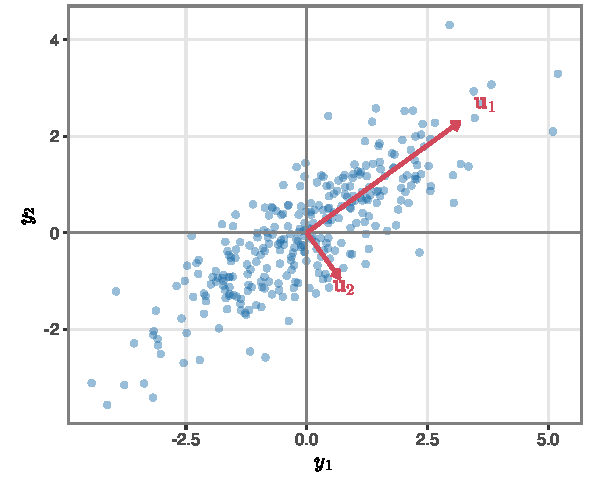
\includegraphics[width=0.5\linewidth]{pca_2d.pdf}
  \caption{PCA of a centered two-dimensional point cloud. The first principal axis $\vu_1$ is the direction of largest variance and $\vu_2$ is orthogonal to it. Each arrow has length $2\sqrt{\lambda_k}$, twice the standard deviation of the data along that axis.}
  \label{fig:pca_2d}
\end{figure}

In practice PCA is computed from the singular value decomposition of the centered data matrix, $\mY=\mA\mD\mB^\top$, without forming $\mS$. Then $\mS=\frac1N\mB\mD^2\mB^\top$, so the eigenvectors are the right singular vectors, $\mU=\mB$, the eigenvalues are $\lambda_k=d_k^2/N$, and the scores are $\mY\mB=\mA\mD$. When only the first few components are needed, truncated or randomized SVD algorithms compute them at a fraction of the cost of the full decomposition.

\subsection{PCA in single-cell analysis}

PCA is a standard first step in most analysis pipelines, and in single-cell RNA-seq it is nearly universal. After normalization and log transformation, the $\sim$20{,}000 genes are filtered to a few thousand highly variable genes, and PCA reduces these to around 30 components. Clustering (Chapter 5), nearest-neighbour graphs and visualizations such as UMAP and t-SNE are then computed in the PC space. This denoises the data, since the discarded components are mostly noise, and makes the downstream computations faster. It is worth considering for any expression analysis whether working with the leading PCs would be better than working with the raw data.

%======================================================================
\section{PCA use case: population structure}
\label{sec:popstruct}
%======================================================================

Two human genomes differ at roughly one position in every thousand, so across the $3\times10^9$ base pairs of the genome a person carries millions of single nucleotide polymorphisms (SNPs) relative to others. Genotyping, by sequencing or with SNP arrays, gives a matrix $\mY\in\{0,1,2\}^{N\times P}$ where $y_{np}$ is the number of copies of the minor allele that individual $n$ carries at SNP $p$, with $P$ in the hundreds of thousands or more. After centering (and usually standardizing) each SNP, PCA of this matrix reveals \emph{population structure}: systematic differences in allele frequencies between groups with different ancestry.

\citet{novembre2008} applied PCA to about 1400 Europeans genotyped at about 200{,}000 SNPs. Plotting the first two PCs, after rotating the axes, reproduces the map of Europe (Figure~\ref{fig:novembre}). Individuals from Spain and Portugal, Italy, France and Switzerland, the British Isles, Scandinavia and south-eastern Europe each occupy the region corresponding to their geography, and barriers to migration such as seas and the Alps appear as gaps. The reason is that for most of the last several thousand years people have mostly had children with partners from nearby. Allele frequencies drift randomly in each place, and limited migration keeps nearby populations similar, so genetic similarity decays with geographic distance. PCA picks up this smooth gradient.

\begin{figure}[tbp]
  \centering
  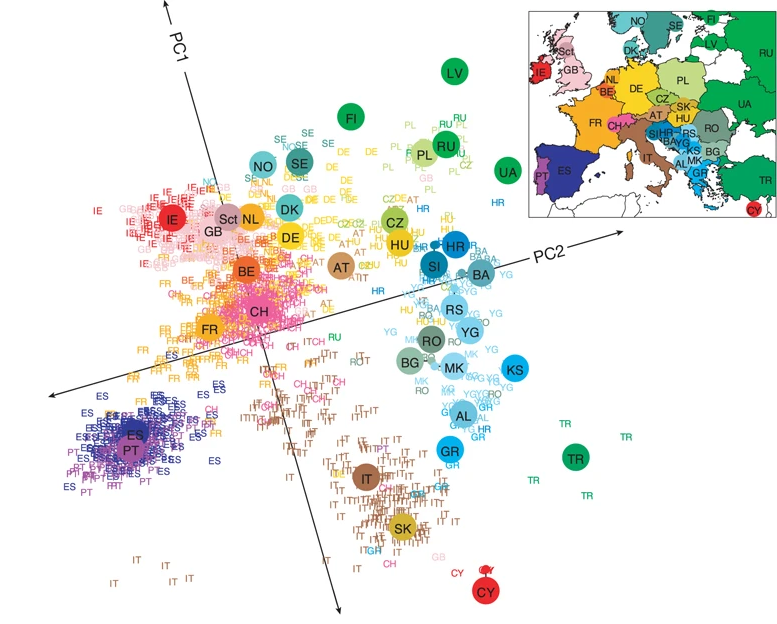
\includegraphics[width=0.75\linewidth]{slides/novembre_pca_europe.png}
  \caption{The first two principal components of genotype data from about 1400 Europeans, coloured by country of origin (labels are country codes; large circles are country medians), with the axes rotated to align with the map (inset). Reproduced from \citet{novembre2008}.}
  \label{fig:novembre}
\end{figure}

Population structure matters because it confounds genetic association studies. A classic example is a study of type 2 diabetes in the Gila River Indian Community in Arizona~\citep{knowler1988}. Individuals carrying the immunoglobulin haplotype $Gm^{3;5,13,14}$ had a much lower prevalence of diabetes at every age (Figure~\ref{fig:knowler}a), suggesting a protective variant. But this haplotype is common in Europeans and rare in Native Americans, and in this community diabetes prevalence rises with the proportion of Native American heritage while the frequency of the haplotype falls (Figure~\ref{fig:knowler}b). The haplotype was a marker of European admixture, and admixture was associated with diabetes risk; when the analysis accounted for heritage, the association largely disappeared. Any variant whose frequency differs between ancestry groups will be associated with any trait that also differs between those groups, for genetic or environmental reasons. A standard correction includes the top genotype PCs as covariates in the association test~\citep{price2006}, which we discuss with genome-wide association studies in Chapter 11.

\begin{figure}[tbp]
  \centering
  \begin{subfigure}[b]{0.38\linewidth}
    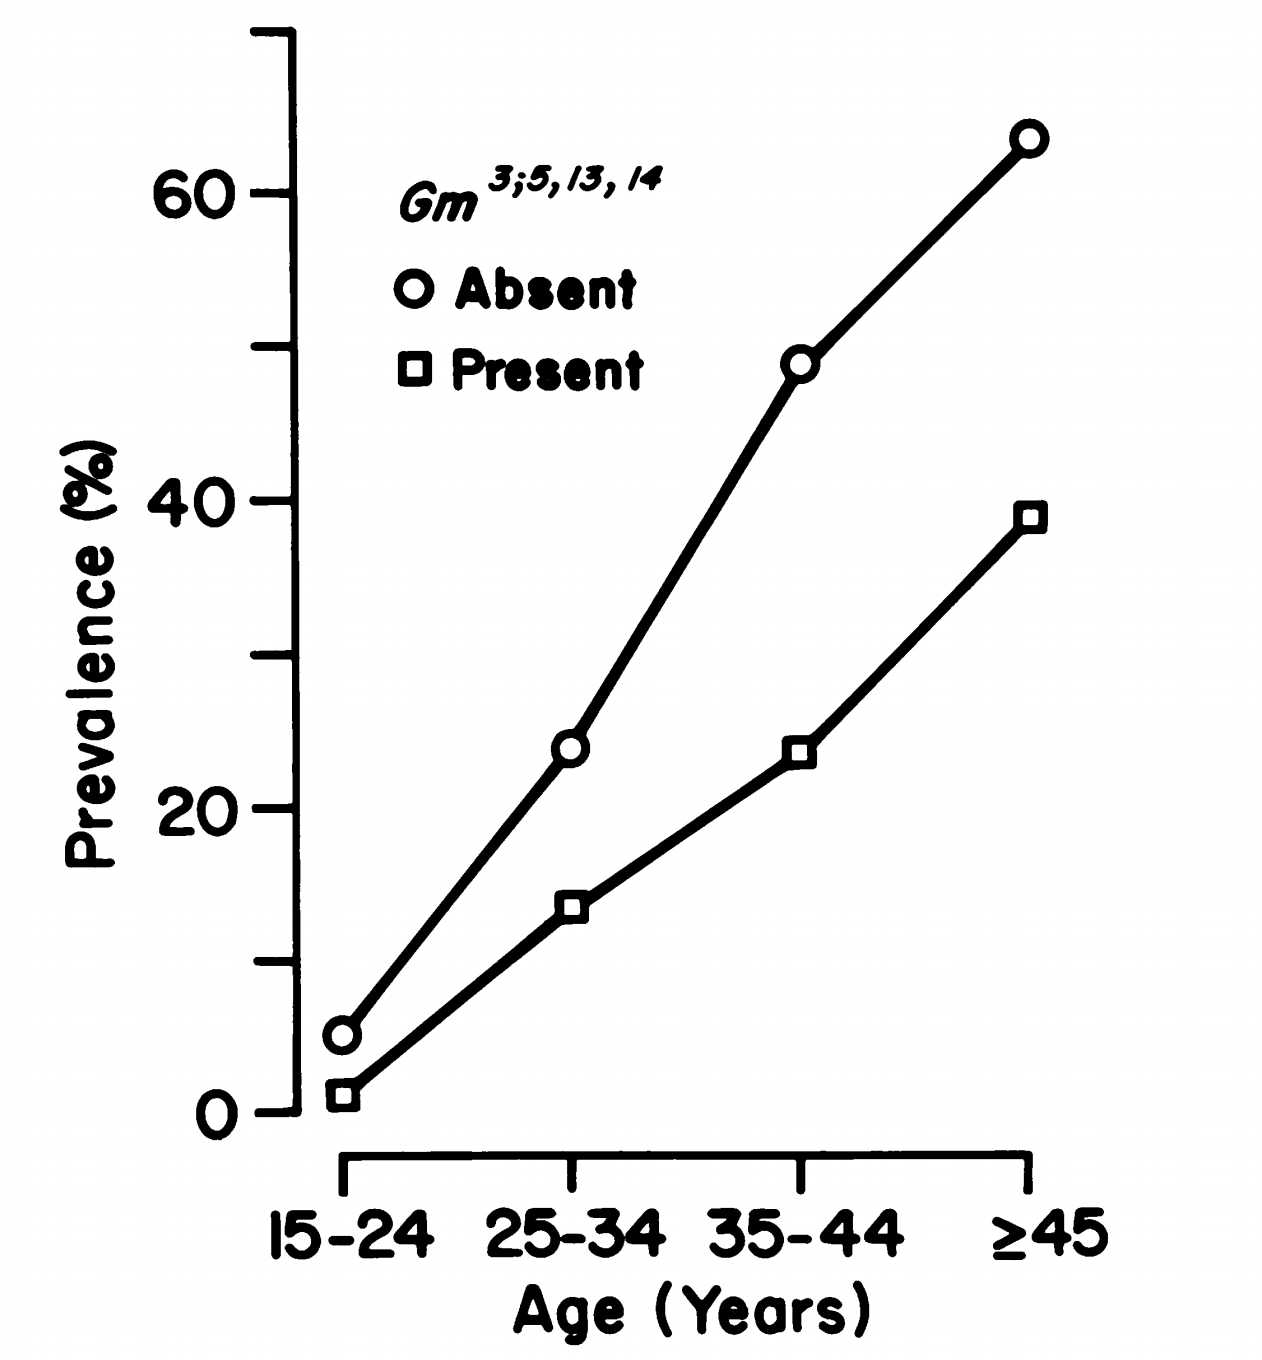
\includegraphics[width=\linewidth]{slides/knowler_fig1.png}
    \caption{}
  \end{subfigure}\hfill
  \begin{subfigure}[b]{0.58\linewidth}
    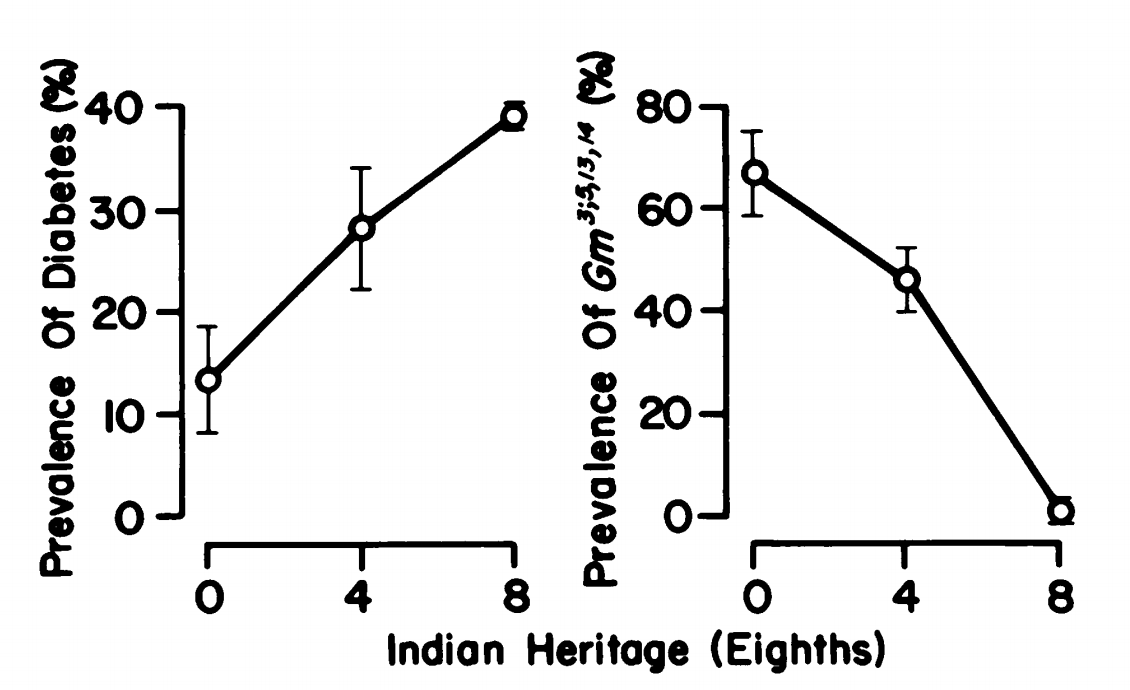
\includegraphics[width=\linewidth]{slides/knowler_fig3.png}
    \caption{}
  \end{subfigure}
  \caption{Confounding by population structure. (a) Prevalence of type 2 diabetes by age among residents of the Gila River Indian Community, by presence of the haplotype $Gm^{3;5,13,14}$. (b) Age-adjusted prevalence ($\pm1$ standard error) of diabetes (left) and of the haplotype (right) by degree of Indian heritage, in eighths. Reproduced from \citet{knowler1988}.}
  \label{fig:knowler}
\end{figure}

%======================================================================
\section{Autoencoders}
\label{sec:ae}
%======================================================================

Recurrent neural networks (Chapter 7) are the deep learning counterpart of hidden Markov models; autoencoders are the deep learning counterpart of matrix factorization. An autoencoder is a neural network trained to reproduce its input. It consists of an \emph{encoder} $f_\phi:\R^P\to\R^K$, which maps a data point $\vy_n$ to a \emph{code} (also called latent representation or embedding) $\vx_n=f_\phi(\vy_n)$, and a \emph{decoder} $g_\theta:\R^K\to\R^P$, which maps the code back to a reconstruction $\hat\vy_n=g_\theta(\vx_n)$ (Figure~\ref{fig:ae}). The parameters $\phi$ and $\theta$ are trained to minimize the reconstruction error,
\begin{equation}
  \min_{\phi,\theta}\sum_{n=1}^N\left\|\vy_n-g_\theta(f_\phi(\vy_n))\right\|^2,
  \label{eq:ae}
\end{equation}
by stochastic gradient descent. Predicting the input from itself is trivial if the network can learn the identity function, so something must stop it from doing so. The simplest constraint is a \emph{bottleneck}, $K\ll P$: the code has fewer dimensions (or, in a convolutional network, fewer channels) than the input, so the network has to find a compressed representation.

\begin{figure}[tbp]
  \centering
  \begin{tikzpicture}[every node/.style={font=\small}, layer/.style={draw, fill=gray!8, minimum width=0.45cm}]
    \node[layer, minimum height=3.2cm] (in) at (0,0) {};
    \node[layer, minimum height=2.3cm] (h1) at (1.8,0) {};
    \node[layer, minimum height=1.1cm, fill=red!15] (code) at (3.6,0) {};
    \node[layer, minimum height=2.3cm] (h2) at (5.4,0) {};
    \node[layer, minimum height=3.2cm] (out) at (7.2,0) {};
    \foreach \a/\b in {in/h1, h1/code, code/h2, h2/out} {
      \draw[gray, dashed] (\a.north east) -- (\b.north west);
      \draw[gray, dashed] (\a.south east) -- (\b.south west);
      \draw[gray, dashed] (\a.north east) -- (\b.south west);
      \draw[gray, dashed] (\a.south east) -- (\b.north west);
    }
    \node[above] at (in.north) {input $\vy_n$};
    \node[above] at (code.north) {code $\vx_n$};
    \node[above] at (out.north) {output $\hat\vy_n$};
    \draw[decorate, decoration={brace, mirror, amplitude=5pt}] (-0.25,-1.8) -- (3.85,-1.8) node[midway, below=6pt] {encoder $f_\phi$};
    \draw[decorate, decoration={brace, mirror, amplitude=5pt}] (3.35,-2.5) -- (7.45,-2.5) node[midway, below=6pt] {decoder $g_\theta$};
    \node[below] at (code.south) {$K\ll P$};
  \end{tikzpicture}
  \caption{An autoencoder. The encoder maps the input $\vy_n\in\R^P$ to a lower-dimensional code $\vx_n\in\R^K$, and the decoder maps the code back to a reconstruction $\hat\vy_n$ of the input. For a denoising autoencoder, the input is a corrupted copy of $\vy_n$ while the reconstruction target is the original.}
  \label{fig:ae}
\end{figure}

\subsection{Linear autoencoders and PCA}

Suppose both encoder and decoder are linear, $\vx_n=\mA\vy_n$ and $\hat\vy_n=\mB\vx_n$ with $\mA\in\R^{K\times P}$ and $\mB\in\R^{P\times K}$. The reconstruction of the whole data matrix is $\hat\mY=\mY\mA^\top\mB^\top$, which has rank at most $K$, and the loss~\eqref{eq:ae} is $\|\mY-\mY\mA^\top\mB^\top\|_F^2$, where $\|\cdot\|_F$ is the Frobenius norm (the square root of the sum of squared entries). By the Eckart-Young theorem no rank-$K$ matrix has smaller squared error than the PCA reconstruction $\mY\mU_K\mU_K^\top$, and the linear autoencoder attains it when $\mB\mA=\mU_K\mU_K^\top$, the orthogonal projection onto the span of the first $K$ principal axes. This holds for $\mB=\mU_K\mG$ and $\mA=\mG^{-1}\mU_K^\top$ with any invertible $\mG\in\R^{K\times K}$, so the decoder spans the PCA subspace but its columns need not be the eigenvectors themselves, the same non-identifiability as in factor analysis. \citet{baldi1989} showed that the loss has no spurious local minima: every local minimum is global and the other stationary points are saddle points. Gradient descent on a linear autoencoder therefore finds the PCA subspace (Figure~\ref{fig:linear_ae}).

\begin{figure}[tbp]
  \centering
  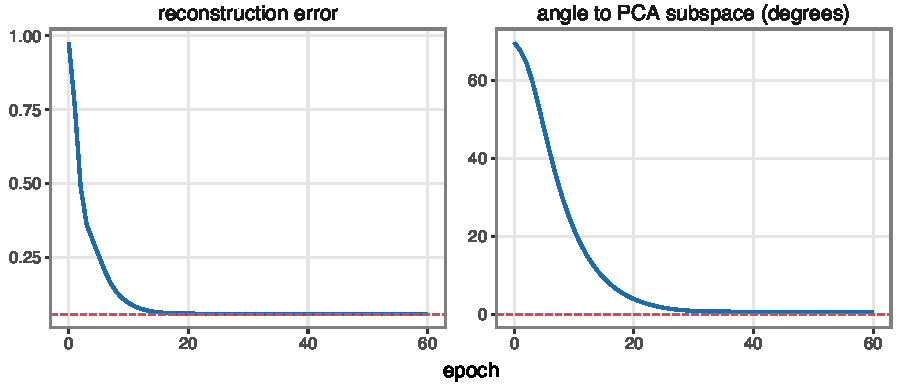
\includegraphics[width=0.9\linewidth]{linear_ae.pdf}
  \caption{A linear autoencoder with $K=3$ trained by minibatch gradient descent on simulated data ($N=2000$, $P=20$, three true factors). Left, the mean squared reconstruction error approaches that of the rank-3 PCA reconstruction (dashed). Right, the largest principal angle between the column space of the decoder $\mB$ and the span of the first three principal axes goes to zero.}
  \label{fig:linear_ae}
\end{figure}

This equivalence has two uses. It gives intuition for what autoencoders do: a nonlinear autoencoder performs a nonlinear analogue of PCA, learning a low-dimensional manifold rather than a subspace~\citep{hinton2006}. And it is a practical way to fit PCA on very large data, since minibatch gradient descent never needs the whole matrix in memory. It also explains the name \emph{latent space} used for autoencoder codes: in the linear case the code is exactly the latent variable $\vx_n$ of probabilistic PCA.

\subsection{Variants}

\begin{itemize}
  \item \emph{Denoising autoencoders}~\citep{vincent2008} corrupt the input, for example by adding noise or setting random entries to zero, and train the network to reconstruct the uncorrupted original, $\min\sum_n\|\vy_n-g_\theta(f_\phi(\tilde\vy_n))\|^2$ with $\tilde\vy_n$ the corrupted copy. The idea is the same as masked language modelling (Chapter 7). Diffusion models~\citep{ho2020} develop the idea formally: they train a denoiser at many known noise levels and use it to generate data.
  \item \emph{Tied} (coupled) autoencoders share parameters between encoder and decoder; in the linear case $\mA=\mB^\top$, as in PCA, where the scores are $\mY\mU_K$ and the reconstruction is $\mY\mU_K\mU_K^\top$. This halves the number of parameters and can help a little.
  \item \emph{Convolutional autoencoders} use convolutions in the encoder and transposed convolutions in the decoder, the operation used by the deconvolutional networks of Chapter 4.
  \item \emph{Variational autoencoders}~\citep{kingma2014} treat the decoder as the generative model $p(\vy_n\mid\vx_n)$ of a latent variable model and the encoder as an \emph{inference network} that outputs an approximate posterior $q(\vx_n\mid\vy_n)$. They are an instance of variational inference, which we cover in a later chapter.
\end{itemize}

%======================================================================
\section{Independent components analysis}
\label{sec:ica}
%======================================================================

\subsection{Heavy-tailed factors}

Independent components analysis keeps the linear model $\vy_n=\mW\vx_n+\veps_n$ but replaces the Gaussian prior on the factors by a heavy-tailed one, with independent components,
\begin{equation}
  p(\vx_n)=\prod_{k=1}^Kp(x_{nk}),
\end{equation}
where $p(x)$ is, for example, a Student-$t$, Laplace ($p(x)\propto e^{-\lambda|x|}$) or Cauchy density. Compared with a Gaussian of the same variance, a heavy-tailed density has more mass near zero and in the tails and less at intermediate values (Figure~\ref{fig:ica}a). This is the same distinction as between the Gaussian and sparse priors on regression coefficients in Chapter 1. Draws from such a prior are \emph{sparse}: for a given data point, most factors are near zero and a few are large.

Figure~\ref{fig:ica}b shows what this does to the data. With Gaussian factors the data form an elliptical cloud. With heavy-tailed factors most points are near the origin, and the rest lie along the directions of individual columns $\vw_k$, because it is rare for two factors to be large at once. The cloud has ``arms'' along the true directions.

\begin{figure}[tbp]
  \centering
  \begin{subfigure}[b]{\linewidth}
    \centering
    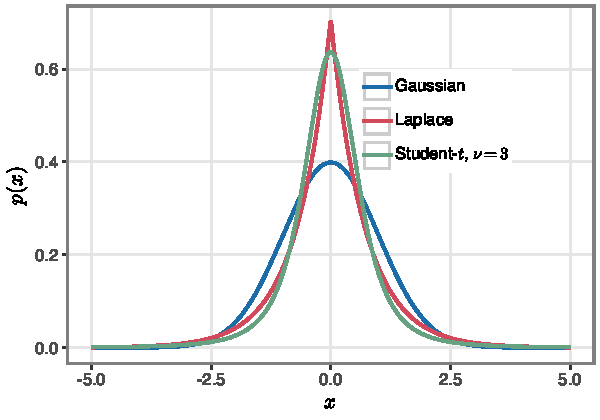
\includegraphics[width=0.5\linewidth]{ica_priors.pdf}
    \caption{}
  \end{subfigure}\\[0.5em]
  \begin{subfigure}[b]{\linewidth}
    \centering
    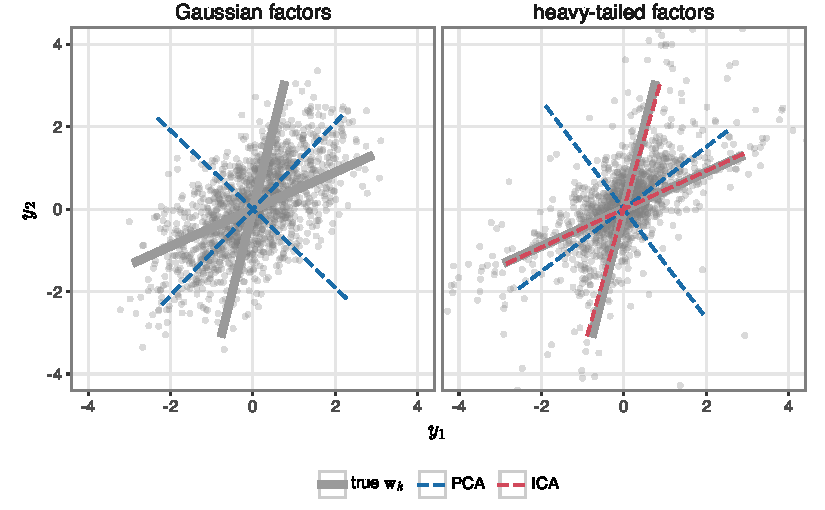
\includegraphics[width=0.85\linewidth]{ica_scatter.pdf}
    \caption{}
  \end{subfigure}
  \caption{Independent components analysis. (a) Gaussian, Laplace and Student-$t$ densities with unit variance; the heavy-tailed densities have more mass near zero and in the tails. (b) Data $\vy_n=\mW\vx_n$ (plus small noise) generated with the same non-orthogonal $\mW$ from Gaussian factors (left) and Student-$t$ factors with 1.5 degrees of freedom (right). Grey lines are the true directions $\vw_1,\vw_2$, blue dashed lines the principal axes, which are orthogonal. With heavy-tailed factors, FastICA (red dashed) recovers the true directions; with Gaussian factors no method can, because the distribution is rotation invariant.}
  \label{fig:ica}
\end{figure}

\subsection{Identifiability}

The heavy-tailed prior resolves the rotational non-identifiability of factor analysis. If $\vx_n\sim\Normal(\vzero,\mI)$ then $\mR^\top\vx_n$ has the same distribution for any orthogonal $\mR$, so $\mW$ and $\mW\mR$ fit equally well. With independent non-Gaussian components, a rotation mixes the components and produces a vector whose entries are no longer independent and whose marginals are closer to Gaussian, by the central limit theorem. The directions $\vw_k$ are then identifiable up to permutation and scaling, provided at most one component is Gaussian~\citep{comon1994}. In Figure~\ref{fig:ica}b the principal axes are orthogonal and do not match the true directions in either panel, while ICA recovers them when the factors are heavy tailed.

Why would biological factors be sparse? Many processes are close to on or off. An immune response is inactive in most cells most of the time and active, to a varying degree, in a few; a cell either is a neuron or is not. A Gaussian factor says every sample is always a little active in every program, which fits such variation poorly.

\subsection{FastICA}

Fitting ICA by maximum likelihood is awkward because the priors are non-standard. The most widely used algorithm is FastICA~\citep{hyvarinen1999,hyvarinen2000}, which is derived from maximizing the non-Gaussianity of the recovered components and works in the noiseless setting with $K=P$ or after reducing to $K$ dimensions by PCA. The data are first \emph{whitened}, $\vz_n=\mLambda_K^{-1/2}\mU_K^\top\vy_n$, so that $\frac1N\sum_n\vz_n\vz_n^\top=\mI_K$. After whitening the remaining unknown is a rotation. For one component, FastICA seeks a unit vector $\vw\in\R^K$ such that $\vw^\top\vz_n$ is as non-Gaussian as possible, using the fixed-point iteration
\begin{equation}
  \vw\leftarrow\frac1N\sum_n\vz_n\,g(\vw^\top\vz_n)-\left[\frac1N\sum_ng'(\vw^\top\vz_n)\right]\vw, \qquad \vw\leftarrow\vw/\|\vw\|,
\end{equation}
where $g$ is a non-linearity such as $g(u)=\tanh(u)$. A fixed-point algorithm repeatedly applies an update until the estimate stops changing; this one is a Newton step and converges quickly. Several components are found together by applying the update to each row of a matrix and re-orthogonalizing the rows after each step. FastICA is fast and has no tuning parameters beyond $K$ and $g$, so it is a reasonable alternative to PCA when sparse, on-off factors are plausible.

%======================================================================
\section{Non-negative matrix factorization}
\label{sec:nmf}
%======================================================================

\subsection{The model}

Many genomic data are non-negative: read counts, normalized expression, mutation counts. Non-negative matrix factorization~\citep{lee1999} approximates a non-negative $\mY\in\R_{\geq0}^{N\times P}$ by $\mX\mW^\top$ with both factors constrained to be non-negative,
\begin{equation}
  \min_{\mX\geq0,\ \mW\geq0}\ \left\|\mY-\mX\mW^\top\right\|_F^2,
  \label{eq:nmf}
\end{equation}
where $\mX\in\R_{\geq0}^{N\times K}$, $\mW\in\R_{\geq0}^{P\times K}$ and the inequalities hold element-wise. Replacing the squared error by the Kullback-Leibler divergence gives the maximum likelihood estimate under a Poisson model for counts, $y_{np}\sim\text{Poisson}(\sum_kx_{nk}w_{pk})$.

Because nothing can be subtracted, each data point has to be built up by adding non-negative parts. NMF therefore tends to give a \emph{parts-based} representation~\citep{lee1999}: each column of $\mW$ is a set of genes that are expressed together (a gene program or ``metagene''~\citep{brunet2004}), and each sample's expression is a non-negative mixture of programs. In PCA, by contrast, loadings and scores have both signs, and a sample can be described as one program minus another, which is harder to interpret. Figure~\ref{fig:nmf} shows simulated data generated from three overlapping non-negative gene programs: NMF recovers the programs, while the principal axes are orthogonal combinations with mixed signs. The non-negativity constraint also removes most of the rotational freedom of factor analysis, since a rotation of non-negative factors generally produces negative entries. A prominent genomic application is the discovery of mutational signatures, the characteristic patterns of somatic mutations left by different mutational processes in cancer genomes~\citep{alexandrov2013}.

\begin{figure}[tbp]
  \centering
  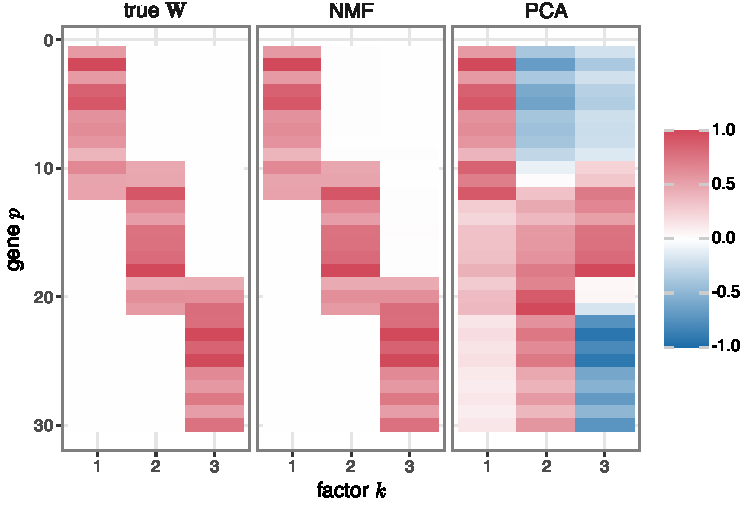
\includegraphics[width=0.75\linewidth]{nmf_vs_pca.pdf}
  \caption{Loadings for simulated non-negative data generated from three overlapping gene programs ($N=300$ samples, $P=30$ genes). Each column is scaled to a maximum absolute value of 1. NMF recovers the programs; PCA loadings mix the programs and have both signs.}
  \label{fig:nmf}
\end{figure}

\subsection{Multiplicative updates}

Problem~\eqref{eq:nmf} is not jointly convex in $\mX$ and $\mW$ but is convex in each given the other. \citet{lee2001} proposed alternating multiplicative updates. The gradient of the objective with respect to $\mX$ is $-2(\mY\mW-\mX\mW^\top\mW)$. A gradient step with an element-wise step size $\eta_{nk}=x_{nk}/(2[\mX\mW^\top\mW]_{nk})$ gives
\begin{equation}
  x_{nk}\leftarrow x_{nk}+\frac{x_{nk}}{[\mX\mW^\top\mW]_{nk}}\left([\mY\mW]_{nk}-[\mX\mW^\top\mW]_{nk}\right)
  = x_{nk}\frac{[\mY\mW]_{nk}}{[\mX\mW^\top\mW]_{nk}},
\end{equation}
and by symmetry
\begin{equation}
  w_{pk}\leftarrow w_{pk}\frac{[\mY^\top\mX]_{pk}}{[\mW\mX^\top\mX]_{pk}}.
\end{equation}
All quantities in the ratios are non-negative, so the updates keep $\mX$ and $\mW$ non-negative without any projection, and \citet{lee2001} showed that the objective never increases. Faster alternatives solve each half as a non-negative least squares problem. As with $K$-means (Chapter 5), the solution depends on the initialization.

\subsection{Integrating single-cell datasets: LIGER}

Single-cell datasets of the same tissue measured with different technologies, in different laboratories or on different days, differ systematically even when they contain the same cell types. These \emph{batch effects} can dominate the variation: a low-dimensional embedding of two datasets combined often separates them by dataset rather than by cell type. LIGER (linked inference of genomic experimental relationships)~\citep{welch2019} integrates datasets with a joint NMF. It is in a sense the opposite of MOFA. In MOFA the samples are shared and each view has its own features; in LIGER each dataset $i=1,\dots,I$ has its own cells $\mY_i\in\R_{\geq0}^{N_i\times P}$ but all datasets measure the same $P$ genes. LIGER therefore uses dataset-specific factors and loadings that are shared up to a dataset-specific perturbation,
\begin{equation}
  \mY_i\approx\mX_i(\mW+\mV_i)^\top,
\end{equation}
with $\mX_i\in\R_{\geq0}^{N_i\times K}$, a shared $\mW\in\R_{\geq0}^{P\times K}$ and dataset-specific $\mV_i\in\R_{\geq0}^{P\times K}$ (Figure~\ref{fig:liger_schematic}). The objective is
\begin{equation}
  \min_{\mX_i,\mV_i,\mW\geq0}\ \sum_{i=1}^I\left\|\mY_i-\mX_i(\mW+\mV_i)^\top\right\|_F^2+\lambda\sum_{i=1}^I\left\|\mX_i\mV_i^\top\right\|_F^2.
  \label{eq:liger}
\end{equation}
Expanding the first term, the residual is $\mY_i-\mX_i\mW^\top-\mX_i\mV_i^\top$. The penalty shrinks the dataset-specific contribution $\mX_i\mV_i^\top$, so the model explains as much of the data as it can with the shared loadings and uses $\mV_i$ only for what the shared part cannot capture. Equivalently, each dataset has its own loadings $\mW_i=\mW+\mV_i$, and the penalty keeps them close to one another; $\lambda$ sets how close. The problem is solved by alternating non-negative least squares.

\begin{figure}[tbp]
  \centering
  \begin{tikzpicture}[every node/.style={font=\small}]
    \foreach \i/\c/\h/\y in {1/blue/1.9/0, 2/red/1.4/-2.6} {
      \draw[fill=\c!25] (0,\y) rectangle (2.4,\y-\h);
      \node at (1.2,\y-\h/2) {$\mY_\i$};
      \node[left] at (0,\y-\h/2) {$N_\i$};
      \node at (2.8,\y-\h/2) {$\approx$};
      \draw[fill=\c!25] (3.2,\y) rectangle (3.8,\y-\h);
      \node at (3.5,\y-\h/2) {$\mX_\i$};
      \node at (4.15,\y-\h/2) {$\times$};
      \node at (4.5,\y-\h/2) {\Large(};
      \draw[fill=black!70] (4.8,\y-\h/2+0.6) rectangle (7.2,\y-\h/2+0.05);
      \node[white] at (6.0,\y-\h/2+0.33) {shared $\mW^\top$};
      \node at (6.0,\y-\h/2-0.12) {$+$};
      \draw[fill=\c!25] (4.8,\y-\h/2-0.3) rectangle (7.2,\y-\h/2-0.85);
      \node at (6.0,\y-\h/2-0.57) {specific $\mV_\i^\top$};
      \node at (7.5,\y-\h/2) {\Large)};
    }
    \node[above] at (1.2,0) {$P$ genes};
    \node[above] at (3.5,0) {$K$};
    \node[above] at (6.0,-0.2) {$P$ genes};
  \end{tikzpicture}
  \caption{LIGER integrates datasets that measure the same $P$ genes in different cells. Each dataset $i$ has its own factors $\mX_i$ and loadings $\mW+\mV_i$, the sum of loadings shared by all datasets and a dataset-specific part. After \citet{welch2019}.}
  \label{fig:liger_schematic}
\end{figure}

After fitting, the factors $\mX_i$ of all datasets live in a common space and serve as the representation of each cell; LIGER further normalizes them across datasets before clustering. Figure~\ref{fig:liger_tsne} shows peripheral blood mononuclear cells profiled with two technologies, Seq-Well and 10x Genomics. In a t-SNE embedding of the LIGER factors (t-SNE and UMAP are nonlinear two-dimensional embeddings discussed in Chapter 5), cells from the two technologies overlap, and the clusters correspond to cell types such as T cells, NK cells, B cells and monocytes, rather than to technology. Integration of this kind works when there is shared biological structure for the model to align; it cannot recover cell types that are present in only one dataset and resemble nothing in the others.

\begin{figure}[tbp]
  \centering
  \begin{subfigure}[b]{0.36\linewidth}
    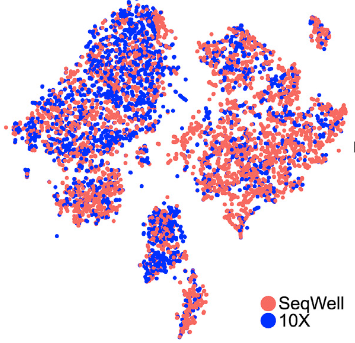
\includegraphics[width=\linewidth]{slides/liger_tsne_technology.png}
    \caption{}
  \end{subfigure}\hfill
  \begin{subfigure}[b]{0.6\linewidth}
    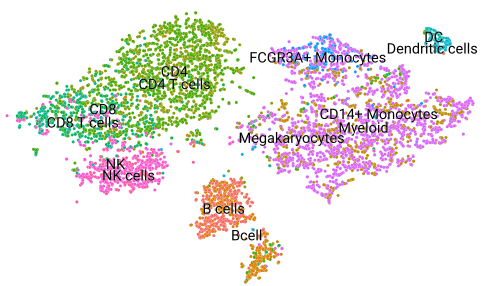
\includegraphics[width=\linewidth]{slides/liger_tsne_celltype.png}
    \caption{}
  \end{subfigure}
  \caption{t-SNE embedding of LIGER factors for peripheral blood cells profiled with Seq-Well and 10x technologies, coloured by (a) technology and (b) cell type label from the original studies. Reproduced from \citet{welch2019}.}
  \label{fig:liger_tsne}
\end{figure}

%======================================================================
\section{Cell type deconvolution of bulk expression}
\label{sec:deconv}
%======================================================================

\subsection{Motivation}

Large patient cohorts, such as The Cancer Genome Atlas, mostly have \emph{bulk} RNA-seq, which measures the summed expression of all cells in a tissue sample. A tumour sample contains cancer cells and also stromal and immune cells, and the immune cells, which may be attacking the tumour or be suppressed by it, are of great clinical interest. \emph{Cell type deconvolution} estimates the proportions of cell types in each bulk sample from its expression profile and a reference expression profile for each cell type. CIBERSORT~\citep{newman2015} made the approach popular and started a large subfield. Its reference profiles came from bulk RNA of experimentally purified cell populations; modern methods typically build them from single-cell RNA-seq, which allows the resolution of the cell types (for example all T cells, or cytotoxic and helper T cells separately) to be chosen \emph{in silico} after the data are generated, rather than fixed by the sorting strategy used to purify the cells.

\begin{figure}[tbp]
  \centering
  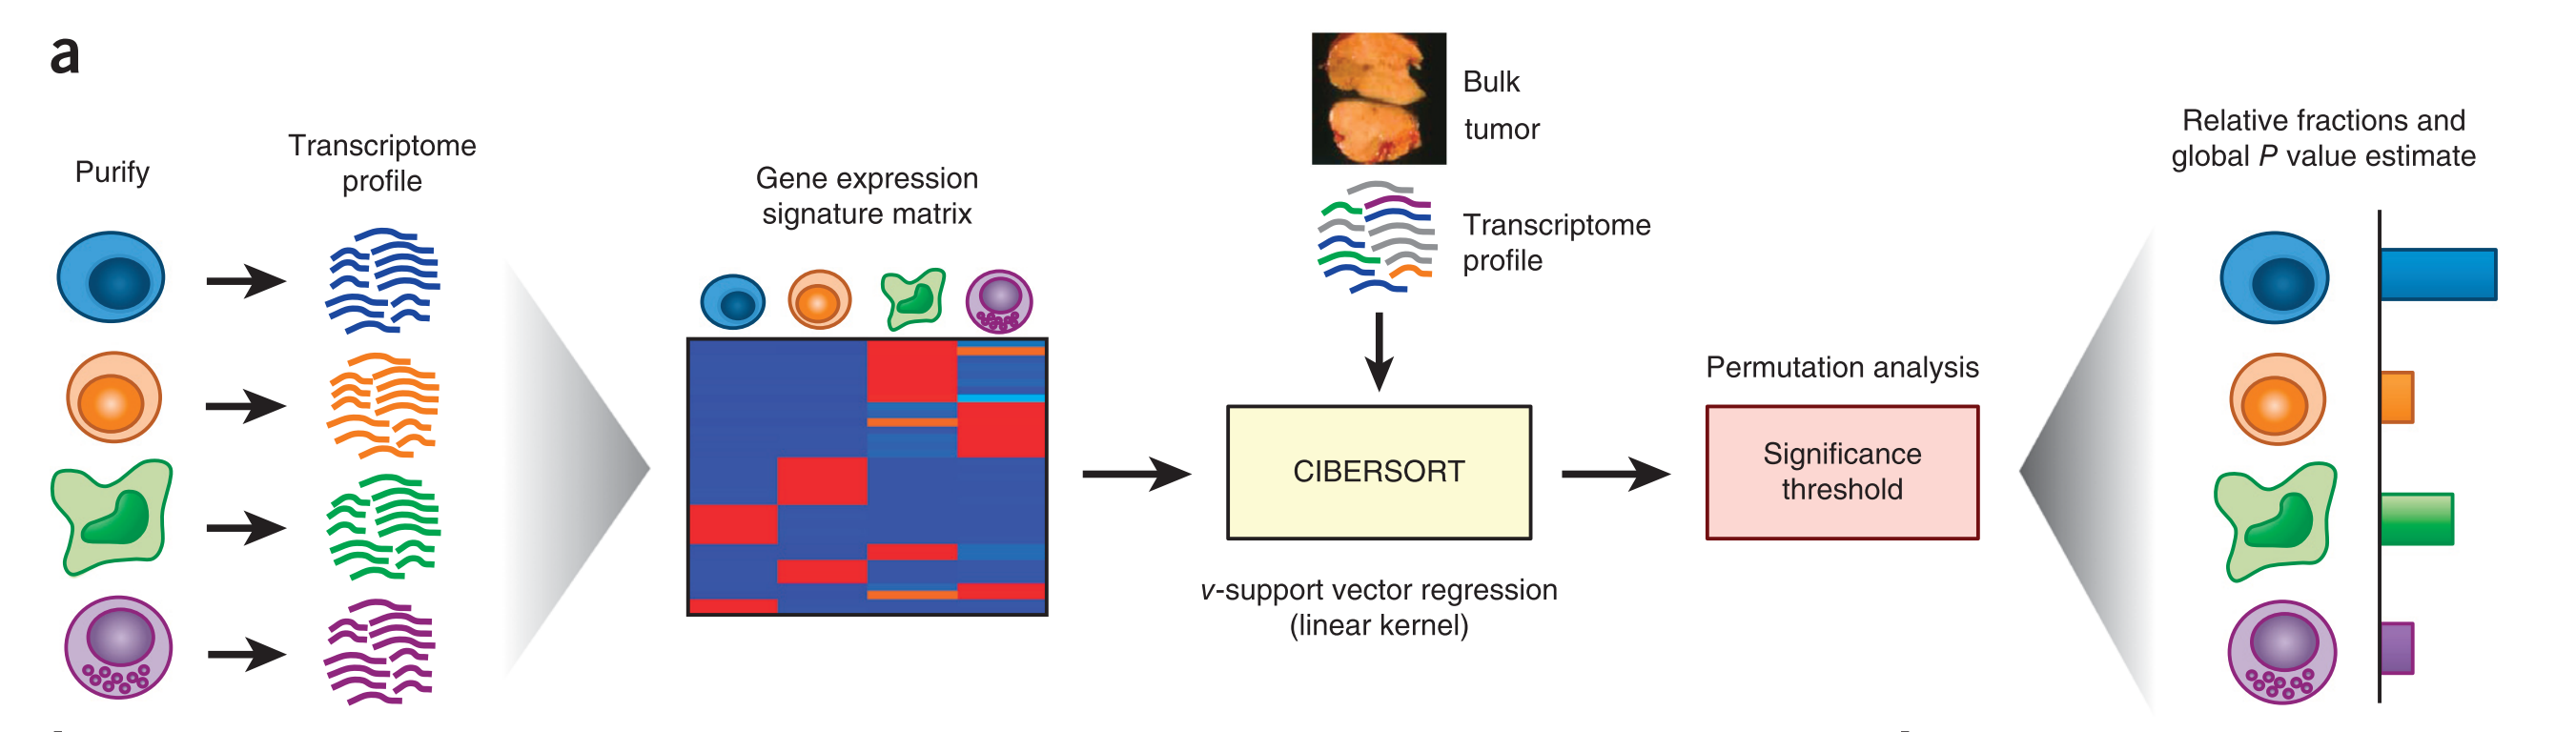
\includegraphics[width=\linewidth]{slides/cibersort_schematic.png}
  \caption{CIBERSORT. Expression profiles of purified cell types form a signature matrix (our $\mW$). The transcriptome of a bulk tumour sample is deconvolved by $\nu$-support vector regression with a linear kernel, giving the relative fractions of the cell types and a $P$ value from a permutation test. Reproduced from \citet{newman2015}.}
  \label{fig:cibersort}
\end{figure}

\subsection{Deconvolution as regression}

Deconvolution has the form of a matrix factorization in which one factor is known. Let $\mY\in\R^{N\times P}$ hold the bulk expression of $P$ genes in $N$ samples, and let $\mW\in\R^{P\times K}$ be the \emph{signature matrix}, with $w_{pk}$ the expression of gene $p$ in cell type $k$ and $K$ the number of cell types. Then
\begin{equation}
  \mY=\mX\mW^\top+\mE, \qquad \vy_n=\mW\vx_n+\veps_n,
\end{equation}
where $x_{nk}$ is the abundance of cell type $k$ in sample $n$, the quantity we want. Since $\mW$ is known, estimating $\vx_n$ is a linear regression for each sample separately, in which the ``data points'' are the $P$ genes and the ``covariates'' are the $K$ columns of $\mW$. Any feature with cell-type-specific signal can be used, for example chromatin accessibility instead of expression.

What makes the problem unusual is the residual $\veps_n$. The signature matrix covers immune and stromal cell types, but a tumour sample also contains cancer cells, whose expression is not in $\mW$ and differs between patients. Their contribution ends up in $\veps_n$, and it is large for the genes the cancer cells express highly. A squared-error loss lets a few genes with large residuals dominate the fit. CIBERSORT instead uses support vector regression, whose loss grows only linearly for large residuals.

\subsection{Support vector regression}

The $\epsilon$-insensitive loss of a residual $r$ is
\begin{equation}
  \ell_\epsilon(r)=\max(0,|r|-\epsilon),
\end{equation}
which is zero inside a ``tube'' $|r|\leq\epsilon$ and grows linearly outside it (Figure~\ref{fig:svr}a). Support vector regression (SVR) for sample $n$ minimizes
\begin{equation}
  \min_{\vx_n,b}\ \frac12\|\vx_n\|^2+C\sum_{p=1}^P\ell_\epsilon\left(y_{pn}-\vw_p^\top\vx_n-b\right),
  \label{eq:svr}
\end{equation}
where $\vw_p^\top$ is row $p$ of $\mW$, $b$ is an intercept and $C>0$ balances the loss against the L2 penalty on $\vx_n$. The lecture slides write the same objective summed over all samples with $C=1$ and no intercept. Compared with squared error, a residual twice as large costs twice as much rather than four times as much, so the fit tolerates a few genes with large errors, such as those dominated by cancer-cell expression (Figure~\ref{fig:svr}b). The absolute loss is the negative log likelihood of Laplace noise, so SVR with $\epsilon=0$ is ridge-penalized least absolute deviation regression, the robust counterpart of ridge regression.

\begin{figure}[tbp]
  \centering
  \begin{subfigure}[b]{0.44\linewidth}
    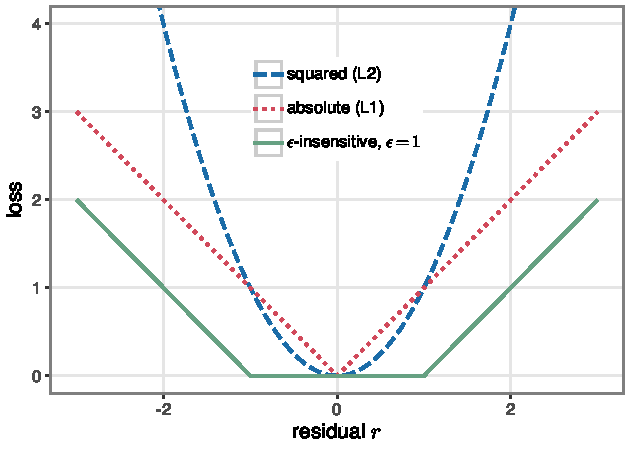
\includegraphics[width=\linewidth]{svr_losses.pdf}
    \caption{}
  \end{subfigure}\hfill
  \begin{subfigure}[b]{0.52\linewidth}
    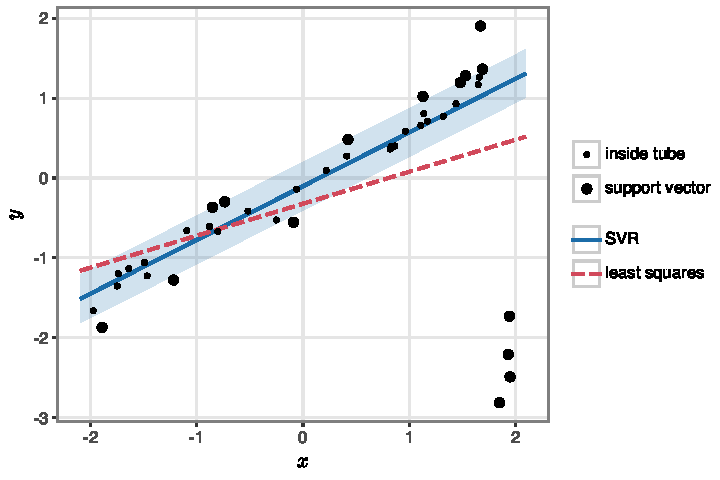
\includegraphics[width=\linewidth]{svr_fit.pdf}
    \caption{}
  \end{subfigure}
  \caption{Support vector regression. (a) Squared, absolute and $\epsilon$-insensitive losses as functions of the residual. (b) Linear SVR with $\epsilon=0.3$ (blue line and tube) and least squares (red dashed) fitted to simulated data with true slope $0.8$ and four outliers at the right. The least-squares slope is pulled down to $0.40$; the SVR slope is $0.67$. Large points are support vectors, on or outside the tube; the fit depends only on them.}
  \label{fig:svr}
\end{figure}

The solution of~\eqref{eq:svr} can be written, through its dual problem, as $\vx_n=\sum_p(a_p-a_p^*)\vw_p$ with dual variables $a_p,a_p^*\in[0,C]$ that are non-zero only for genes whose residual is on or outside the tube. These genes are the \emph{support vectors}. Genes fitted to within $\epsilon$ do not affect the solution at all. The lasso is sparse in the coefficients; SVR is sparse in the data points.

Choosing $\epsilon$ requires knowing the scale of the residuals. $\nu$-SVR~\citep{scholkopf2000} replaces $\epsilon$ by a parameter $\nu\in(0,1]$ and estimates $\epsilon\geq0$ as part of the optimization,
\begin{equation}
  \min_{\vx_n,b,\epsilon\geq0}\ \frac12\|\vx_n\|^2+C\left(\nu\epsilon+\frac1P\sum_{p=1}^P\ell_\epsilon\left(y_{pn}-\vw_p^\top\vx_n-b\right)\right).
\end{equation}
\citet{scholkopf2000} showed that $\nu$ is an upper bound on the fraction of data points outside the tube and a lower bound on the fraction of support vectors, which makes it easier to set than $\epsilon$. CIBERSORT standardizes the mixture and the signature matrix, fits linear $\nu$-SVR with $\nu\in\{0.25,0.5,0.75\}$, keeps the fit with the smallest root mean squared error between the observed and reconstructed mixture, sets negative coefficients to zero and normalizes the rest to sum to one. The result is the relative proportion of each cell type among those in the signature matrix; for a tumour these are fractions of the immune cells, not of all cells. A permutation test, comparing the fit with fits to random mixtures, gives a $P$ value for whether the sample contains any of the signature cell types.

\subsection{Comparison with other regression methods}

SVR is one of several linear regression methods that differ only in their loss and regularization (Table~\ref{tab:regression_losses}). All can be fitted by convex optimization.

\begin{table}[tbp]
  \centering
  \caption{Linear regression methods as combinations of a loss on the residuals and a penalty on the coefficients.}
  \label{tab:regression_losses}
  \begin{tabular}{llll}
    \toprule
    Method & Loss & Regularization & Sparse in \\
    \midrule
    Ordinary least squares & L2 & none & -- \\
    Ridge regression & L2 & L2 & -- \\
    Lasso & L2 & L1 & coefficients \\
    Elastic net & L2 & L1 and L2 & coefficients \\
    SVR with $\epsilon=0$ & L1 & L2 & data points \\
    $\epsilon$-SVR, $\nu$-SVR & $\max(0,|r|-\epsilon)$ & L2 & data points \\
    \bottomrule
  \end{tabular}
\end{table}

Figure~\ref{fig:deconv_sim} compares the losses on simulated deconvolution data. Each of 40 bulk samples is a mixture of five cell types with known signatures, diluted by a sample-specific ``tumour'' profile, not in the signature matrix, that is highly expressed in a random 10\% of genes. Least squares is pulled by the tumour-dominated genes and the proportions it estimates are poor. Least absolute deviation and CIBERSORT-style $\nu$-SVR, whose losses grow linearly, estimate them accurately.

\begin{figure}[tbp]
  \centering
  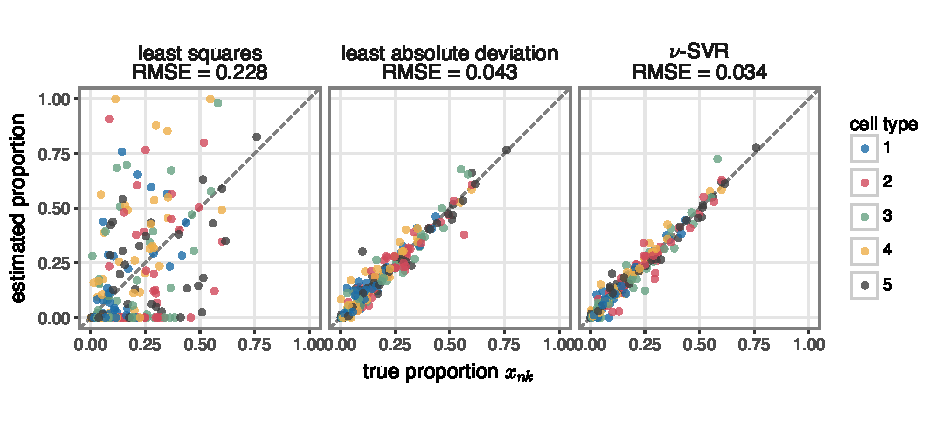
\includegraphics[width=\linewidth]{deconvolution_sim.pdf}
  \caption{Simulated deconvolution. Bulk profiles of $P=400$ genes are mixtures of $K=5$ cell types (immune fraction 30--70\%) plus an unmodelled tumour profile with very high expression of 40 random genes. Estimated against true cell type proportions for least squares, least absolute deviation and $\nu$-SVR, each with negative coefficients set to zero and normalized to sum to one.}
  \label{fig:deconv_sim}
\end{figure}

\subsection{Validation and application}

\citet{newman2015} validated CIBERSORT on blood samples whose composition was measured independently with a Coulter counter, an instrument that counts and sizes cells. The estimated fractions of lymphocytes, monocytes and neutrophils (polymorphonuclear cells, PMNs) correlated with the measured fractions with $R=0.91$ (Figure~\ref{fig:cibersort_validation}). The overall correlation is helped by the large differences between cell types; the agreement within a single cell type, for example the monocytes, is weaker.

\begin{figure}[tbp]
  \centering
  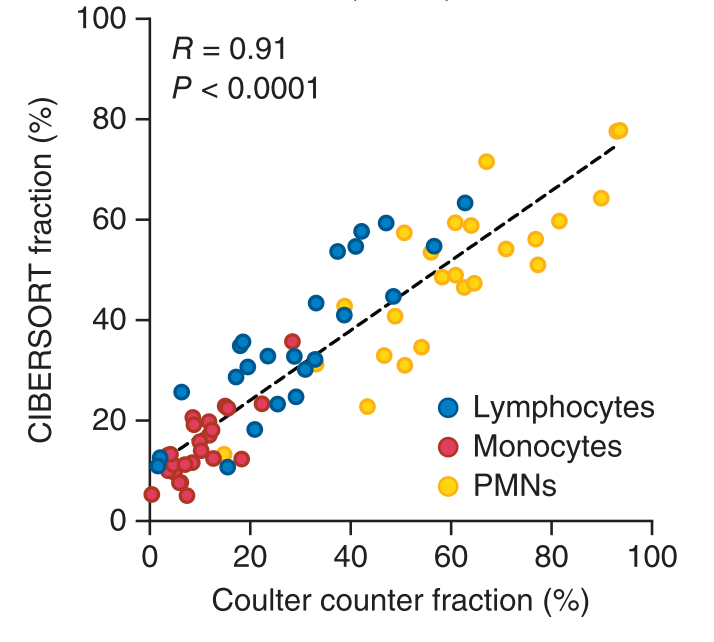
\includegraphics[width=0.45\linewidth]{slides/cibersort_coulter.png}
  \caption{CIBERSORT estimates against Coulter counter measurements of lymphocyte, monocyte and neutrophil (PMN) fractions in blood samples. Reproduced from \citet{newman2015}.}
  \label{fig:cibersort_validation}
\end{figure}

\citet{gentles2015} then applied CIBERSORT to thousands of tumour expression profiles from 25 malignancies with patient survival data. The estimated immune composition differs between cancer types (Figure~\ref{fig:gentles}a). In several blood cancers B cells dominate, because the cancer cells are themselves B cells; brain tumours are rich in monocytes and macrophages. Relating the estimated fractions to survival (Figure~\ref{fig:gentles}b), $\gamma\delta$ T cells were the population most associated with favourable outcomes across cancers, and neutrophils (PMNs) with adverse outcomes. The immune composition of a tumour, estimated computationally from existing bulk data, is thus predictive of prognosis.

\begin{figure}[tbp]
  \centering
  \begin{subfigure}[b]{\linewidth}
    \centering
    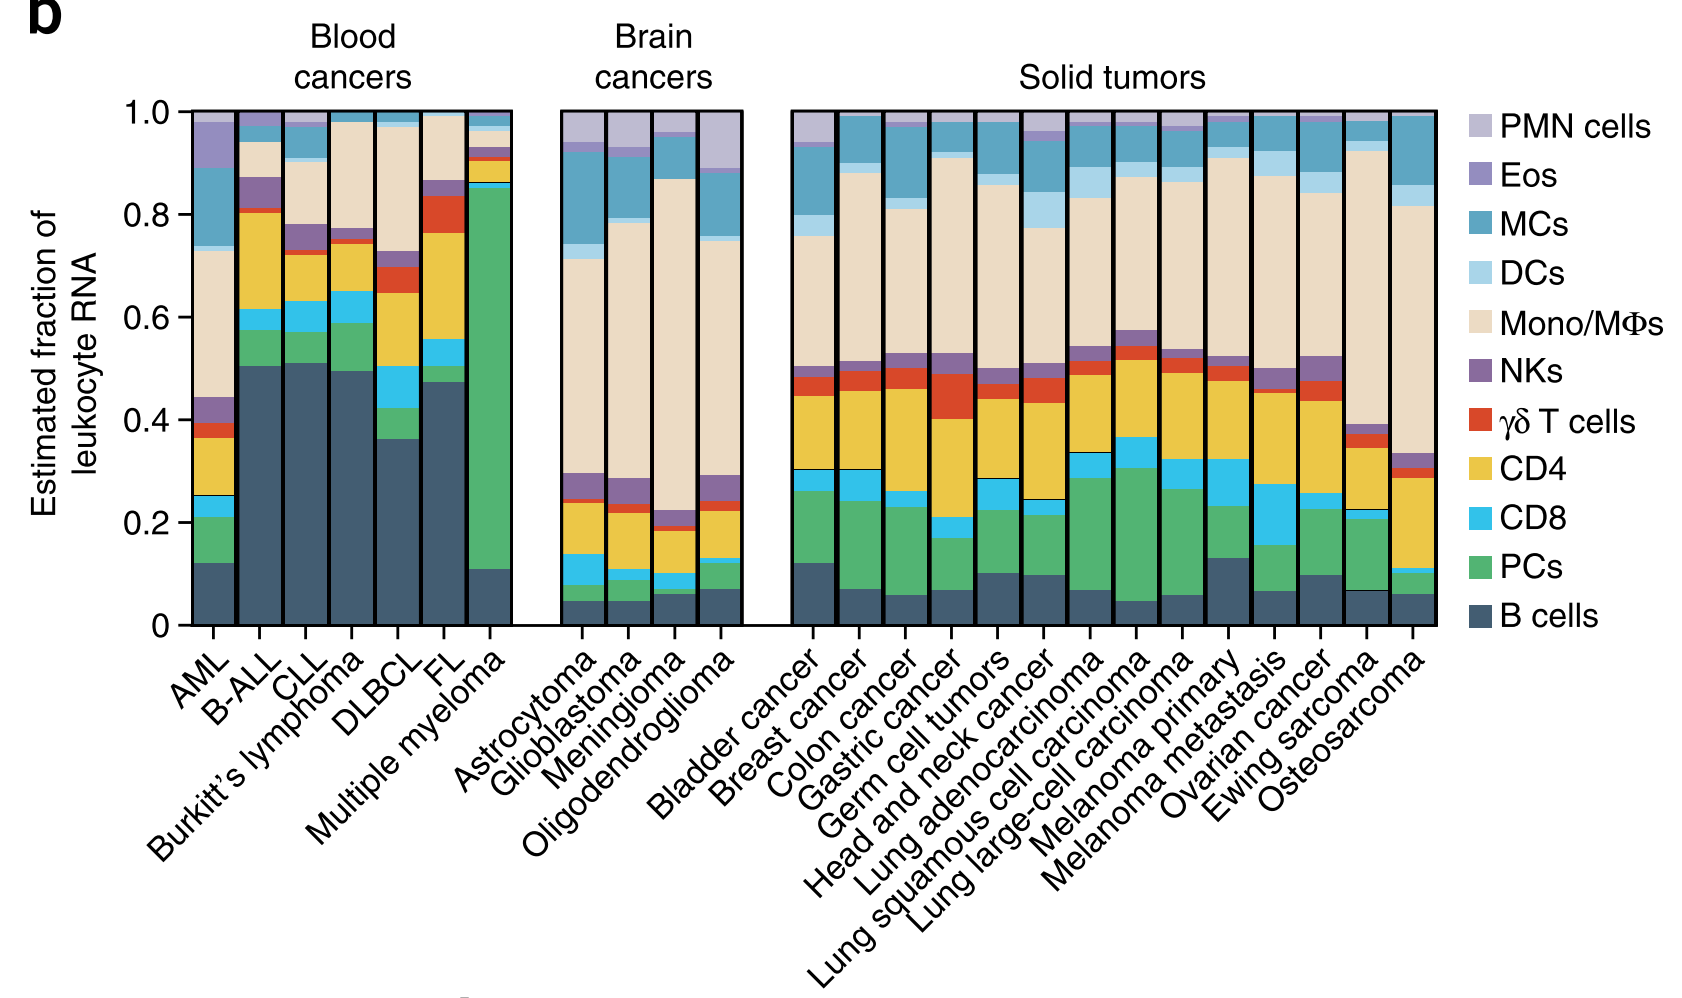
\includegraphics[width=0.85\linewidth]{slides/gentles_fractions.png}
    \caption{}
  \end{subfigure}\\[0.5em]
  \begin{subfigure}[b]{\linewidth}
    \centering
    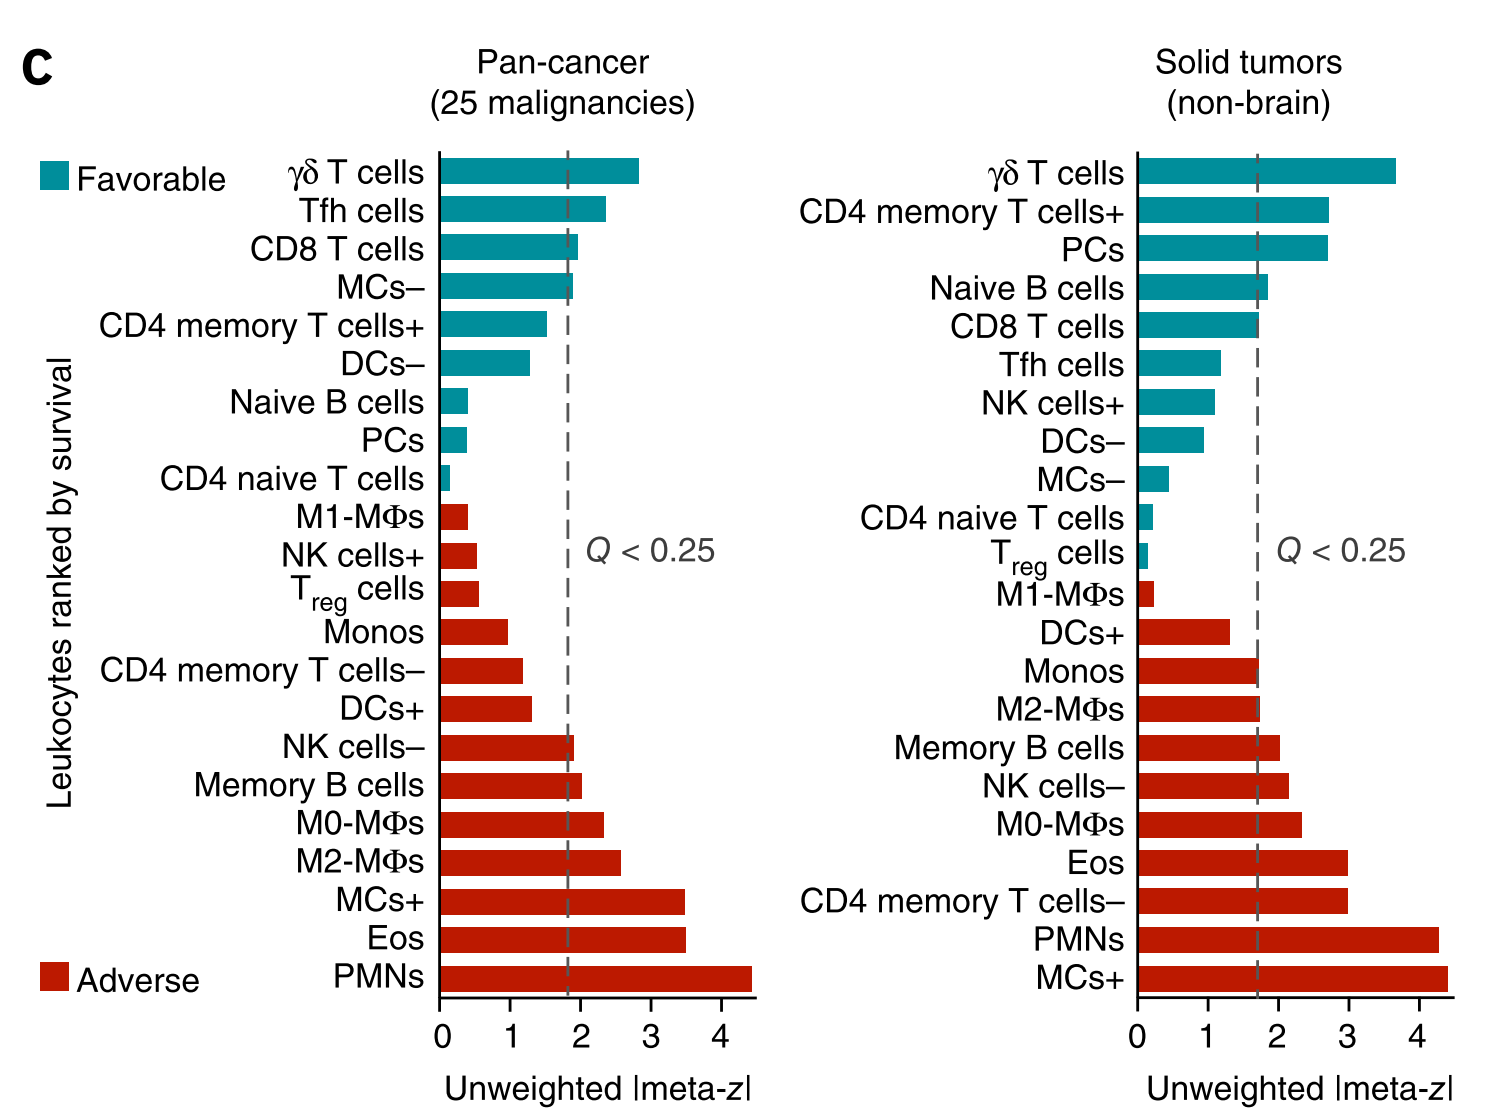
\includegraphics[width=0.75\linewidth]{slides/gentles_survival.png}
    \caption{}
  \end{subfigure}
  \caption{Immune composition of human cancers estimated by CIBERSORT. (a) Estimated fractions of leukocyte RNA by cancer type (panel b of the original). (b) Leukocyte populations ranked by the association of their estimated abundance with survival (meta-analysis $|z|$ score) across 25 malignancies and across non-brain solid tumours; teal, favourable; red, adverse (panel c of the original). MCs, mast cells; PCs, plasma cells; DCs, dendritic cells; M$\Phi$s, macrophages; $+$ and $-$ denote activated and resting states. Reproduced from \citet{gentles2015}.}
  \label{fig:gentles}
\end{figure}

%======================================================================
\section{Summary}
%======================================================================

\begin{itemize}
  \item Matrix factorization models represent each data point as a linear combination of $K$ underlying factors, $\mY\approx\mX\mW^\top$. They are used for dimensionality reduction, visualization, denoising, imputation, removing hidden confounders and integrating datasets.
  \item Factor analysis is the probabilistic base model, with Gaussian factors and feature-specific noise. Integrating out the factors gives a Gaussian with low-rank-plus-diagonal covariance $\mW\mW^\top+\mPsi$, fitted by gradient-based maximum likelihood or by EM. The loadings are identified only up to rotation.
  \item MOFA extends factor analysis to several data types measured on the same samples, with a shared factor matrix and view-specific loadings whose relevance to each view is learned by an ARD prior.
  \item Probabilistic PCA assumes the same noise variance for all features. Its maximum likelihood solution comes from the eigendecomposition of the sample covariance, and PCA is its limit as the noise variance goes to zero. The Marchenko-Pastur law describes the eigenvalues expected from noise and helps choose $K$.
  \item PCA of genotype data reveals population structure, which confounds genetic association studies unless accounted for.
  \item ICA uses heavy-tailed factors, which makes the directions identifiable and suits on-or-off biological programs. NMF constrains both factors to be non-negative and gives parts-based representations; LIGER uses a joint NMF to integrate single-cell datasets.
  \item Autoencoders are the deep learning counterpart; a linear autoencoder learns the PCA subspace.
  \item Cell type deconvolution is a matrix factorization with known loadings. CIBERSORT uses $\nu$-support vector regression, whose robust loss tolerates expression from cell types missing from the signature matrix.
\end{itemize}

%======================================================================
\section*{Exercises}
%======================================================================

\begin{enumerate}
  \item Derive the posterior~\eqref{eq:fa_estep} of the factors in factor analysis from the joint Gaussian distribution of $(\vx_n,\vy_n)$, using the formula for the conditional distribution of a partitioned Gaussian. Show that it agrees with the completing-the-square derivation in the text by using the Woodbury identity.
  \item Implement EM for factor analysis and check that the log likelihood~\eqref{eq:fa_loglik} increases at each iteration. Modify the E- and M-steps to handle missing entries of $\mY$.
  \item Substitute $\hat\mW$ from~\eqref{eq:ppca_ml} into the probabilistic PCA log likelihood and show that the maximizing $\sigma^2$ is the average of the discarded eigenvalues.
  \item Show that the MAP estimate of $\mW$ in probabilistic PCA with the prior $\vw_k\sim\Normal(\vzero,\alpha_k^{-1}\mI)$ on each column, for fixed $\vx_n$, is a ridge regression of $\vy$ on $\vx$. What happens to column $k$ as $\alpha_k\to\infty$?
  \item Verify that the multiplicative update for $\mW$ in NMF is a gradient step with an appropriate element-wise step size, and show that an entry of $\mX$ or $\mW$ that reaches zero stays at zero.
  \item Simulate bulk mixtures as in Figure~\ref{fig:deconv_sim} but without the tumour component. Compare least squares, non-negative least squares and $\nu$-SVR. Which assumption of CIBERSORT does this experiment test, and what changes when a cell type present in the mixture is missing from the signature matrix?
\end{enumerate}

\bibliographystyle{abbrvnat}
\bibliography{../chapter08/chapter08}
\endgroup

% Generated wrapper: chapter 09 with its own figure path, macros and bibliography.
\graphicspath{{../chapter09/figures/}}
\makeatletter\def\input@path{{../chapter09/}}\makeatother
\begingroup
% Chapter 9: biological networks.
% Requires: amsmath, amssymb, bm, graphicx, booktabs, subcaption,
% tikz (arrows.meta, positioning, calc, decorations.pathreplacing, fit, shapes.geometric), natbib.
% Computed figures and figures/network_stats.tex are produced by scripts/make_figures.py;
% figures/slides/ holds figures taken from the lecture slides.

\providecommand{\R}{\mathbb{R}}
\providecommand{\E}{\mathbb{E}}
\providecommand{\Normal}{\mathcal{N}}
\providecommand{\argmax}{\operatorname*{arg\,max}}
\providecommand{\argmin}{\operatorname*{arg\,min}}
\providecommand{\vy}{\mathbf{y}}
\providecommand{\vx}{\mathbf{x}}
\providecommand{\mX}{\mathbf{X}}
\providecommand{\mI}{\mathbf{I}}
\providecommand{\vb}{\boldsymbol{\beta}}
\providecommand{\veps}{\boldsymbol{\epsilon}}
\providecommand{\vp}{\mathbf{p}}
\providecommand{\vg}{\mathbf{g}}
\providecommand{\ind}{\mathbf{1}}
\providecommand{\mA}{\mathbf{A}}
\providecommand{\mTheta}{\boldsymbol{\Theta}}
\providecommand{\mSigma}{\boldsymbol{\Sigma}}
\providecommand{\hSigma}{\hat{\boldsymbol{\Sigma}}}
\providecommand{\mGamma}{\boldsymbol{\Gamma}}
\providecommand{\veta}{\boldsymbol{\eta}}
\providecommand{\vc}{\mathbf{c}}
\providecommand{\vz}{\mathbf{z}}
\providecommand{\vpi}{\boldsymbol{\pi}}
\providecommand{\tr}{\operatorname{tr}}
\providecommand{\cor}{\operatorname{cor}}
\providecommand{\Cov}{\operatorname{Cov}}
\providecommand{\Var}{\operatorname{Var}}
\providecommand{\Bern}{\operatorname{Bernoulli}}
\providecommand{\Cat}{\operatorname{Categorical}}
\providecommand{\Dir}{\operatorname{Dirichlet}}
\providecommand{\indep}{\perp\!\!\!\perp}

\input{figures/network_stats.tex}

\providecommand{\chaptertoc}{}
\chapter{Biological networks}
\label{ch:networks}
\chaptertoc

``Tell me with whom you consort and I will tell you who you are,'' wrote Goethe in his \textit{Maxims and Reflections}. Much of network biology rests on the same idea, often called \emph{guilt by association}: the function of a gene, protein or metabolite can be inferred from the other entities it is connected to. A network, or graph, is a set of nodes and a set of edges between pairs of nodes. In biology the word ``network'' is used for many different things, and the nodes and edges mean different things in each case. On meeting a network in a paper, the first question to ask is what kind of network it is: what are the nodes, what does an edge mean, is it directed, and how was it measured or inferred?

This chapter has three parts. The first surveys the main kinds of biological network: gene regulatory, protein-protein interaction, genetic interaction, metabolic and signaling networks. The second shows how to estimate an undirected network from gene expression data using partial correlations and the graphical lasso, and how to share information when estimating networks for many related tissues. The third treats a network as data in its own right: summary properties from graph theory, and probabilistic models of network structure, the stochastic blockmodel and its mixed membership extension.

%======================================================================
\section{Kinds of biological network}
\label{sec:network_types}
%======================================================================

\subsection{Gene regulatory networks}

Earlier chapters described how transcription factors (TFs) bind DNA near a gene's promoter and increase or decrease its transcription. TFs are proteins, encoded by genes, so their own expression must also be regulated. A TF may activate a set of target genes, some of which are themselves TFs that activate further targets, and some targets feed back to regulate the TF that started the cascade (Figure~\ref{fig:grn_schematic}). Negative feedback of this kind prevents runaway overexpression. The result is a \emph{gene regulatory network} (GRN), in which nodes are genes and a directed edge $A\to B$ means that the product of gene $A$ regulates the expression of gene $B$. Edges are signed: by convention an ordinary arrow denotes activation (up-regulation) and a bar-headed arrow denotes repression (down-regulation).

\begin{figure}[tbp]
  \centering
  \begin{tikzpicture}[>=Stealth, every node/.style={font=\small},
      gene/.style={draw, rounded corners, minimum width=1.6cm, minimum height=0.6cm, fill=blue!8}]
    \node[gene, fill=orange!25] (tf) at (0,0) {TF};
    \node[gene] (a) at (3.2,1.1) {gene A};
    \node[gene] (b) at (3.2,0) {gene B};
    \node[gene, fill=orange!25] (c) at (3.2,-1.1) {gene C (TF)};
    \node[gene] (d) at (6.6,-0.5) {gene D};
    \node[gene] (e) at (6.6,-1.7) {gene E};
    \draw[->, thick] (tf) -- (a);
    \draw[->, thick] (tf) -- (b);
    \draw[->, thick] (tf) -- (c);
    \draw[->, thick] (c) -- (d);
    \draw[-{Bar[width=6pt]}, thick] (c) -- (e);
    \draw[-{Bar[width=6pt]}, thick, red!70!black] (c.south) to[out=-100, in=-90, looseness=1.3] node[below, pos=0.5] {negative feedback} (tf.south);
  \end{tikzpicture}
  \caption{A gene regulatory network. A transcription factor (TF) activates genes A, B and C. Gene C encodes another TF, which activates D, represses E, and represses the first TF, closing a negative feedback loop. Ordinary arrows denote activation, bar-headed arrows repression.}
  \label{fig:grn_schematic}
\end{figure}

The classical way to map a GRN is one gene at a time: knock down or knock out a gene and measure how the expression of other genes changes. Pooled CRISPR screens with single-cell RNA-seq readout, such as Perturb-seq~\citep{dixit2016} and CROP-seq~\citep{datlinger2017}, scale this up. A pool of cells is transduced with a library of guide RNAs so that each cell carries, typically, one perturbation that knocks down (or activates) one gene. The guide identity is recorded in each cell's sequencing library, and single-cell RNA-seq then measures the downstream effect on the whole transcriptome. Figure~\ref{fig:dixit} shows a regulatory network among immune TFs inferred from such a screen in dendritic cells. Early screens perturbed tens to hundreds of genes; genome-scale Perturb-seq has since perturbed every expressed gene in a cell line~\citep{replogle2022}.

\begin{figure}[tbp]
  \centering
  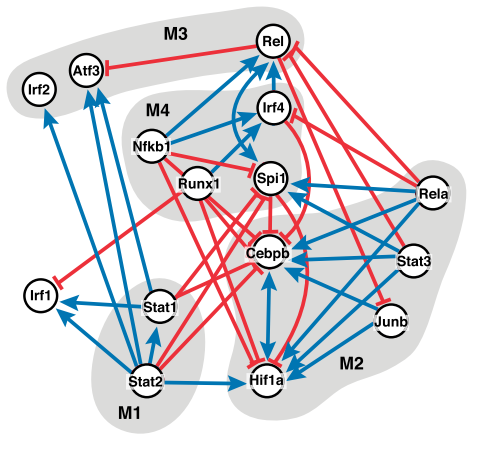
\includegraphics[width=0.5\linewidth]{slides/dixit_perturbseq_network.png}
  \caption{A regulatory network among transcription factors in mouse dendritic cells stimulated with lipopolysaccharide, inferred from a Perturb-seq screen. Blue arrows denote activation and red bar-headed arrows repression; grey regions mark modules M1--M4 of co-functional regulators. Reproduced from \citet{dixit2016}.}
  \label{fig:dixit}
\end{figure}

The readout in these experiments is almost always RNA. Protein levels can be measured for far fewer genes, and some regulation acts on translation or on splicing (Section~\ref{sec:te_ir}), so RNA is not an ideal readout, but it is the one we can measure most completely. Inferring a causal GRN remains hard even with perturbation data. Of the roughly 20{,}000 human protein-coding genes perhaps 8{,}000 are expressed in a given cell type, so the GRN is in principle an $8000\times 8000$ matrix of regulatory effects.

An older strategy reduces the number of parameters in two steps. Genes are first grouped into \emph{modules}, clusters of co-expressed genes, by clustering or by a matrix factorization such as non-negative matrix factorization (Chapter 8) that lets modules share genes. A network is then inferred between modules, or from regulators to modules, rather than between individual genes. Module networks~\citep{segal2003} learned regulators of yeast modules with probabilistic graphical models from observational expression data. \citet{mostafavi2018} applied a similar approach to RNA-seq from the aging human brain, inferring a network of a few tens of modules and linking some of them to amyloid and tau pathology and to cognitive decline. Bayesian network learning of this kind has become less common as perturbation data have grown.

\subsection{Protein-protein interaction networks}

To many biologists ``network'' means a \emph{protein-protein interaction} (PPI) network. The nodes are proteins and an undirected edge means that the two proteins physically bind. Proteins often act in complexes: RNA polymerase II, for example, transcribes DNA to RNA together with a large set of general transcription factors and the Mediator complex, all physically associated with it. Experimental methods usually start from one protein and find its partners, so interaction maps are assembled from many labor-intensive experiments. The results are collected in databases, of which the largest are BioGRID~\citep{stark2006} and STRING~\citep{szklarczyk2019}. STRING also includes predicted functional associations, for example from co-expression and text mining, not only physical binding.

PPI networks are best thought of as having a high false negative rate and a modest false positive rate. An edge in a curated database usually reflects a real interaction, but many true interactions are missing because nobody has tested them, and well-studied proteins have more recorded partners than less-studied ones. Figure~\ref{fig:scz} shows an example network built around genes associated with schizophrenia, which combined known interactions with several hundred newly predicted ones~\citep{ganapathiraju2016}.

\begin{figure}[tbp]
  \centering
  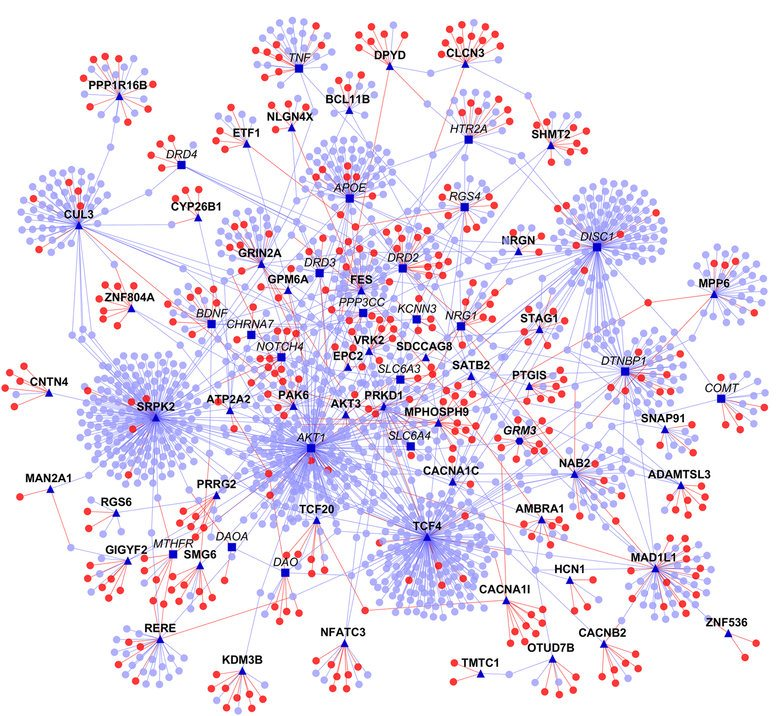
\includegraphics[width=0.65\linewidth]{slides/schizophrenia_interactome.png}
  \caption{A protein-protein interaction network centered on genes associated with schizophrenia (labelled nodes). Known interactions are combined with interactions predicted computationally. Reproduced from \citet{ganapathiraju2016}.}
  \label{fig:scz}
\end{figure}

\paragraph{Yeast two-hybrid screens.} The yeast two-hybrid (Y2H) assay~\citep{fields1989} tests whether two proteins X and Y bind. It uses the yeast transcription factor Gal4, which has two separable parts: a DNA binding domain (BD) that recognizes an upstream activating sequence (UAS), and an activation domain (AD) that recruits the transcriptional machinery. Neither part alone activates transcription. The ``bait'' protein X is fused to the BD and the ``prey'' protein Y to the AD, each expressed from its own plasmid. If X and Y interact, they bring the BD and AD together at the UAS and a reporter gene is transcribed, for example one needed for growth on a selective medium (Figure~\ref{fig:y2h}). Screening a bait against a library of prey reveals its binding partners.

\begin{figure}[tbp]
  \centering
  \begin{tikzpicture}[>=Stealth, every node/.style={font=\small}]
    % plasmids
    \draw[thick] (0,3.0) circle (0.55);
    \draw[line width=3pt, black] (0,3.0) ++(60:0.55) arc (60:110:0.55);
    \draw[line width=3pt, gray] (0,3.0) ++(115:0.55) arc (115:200:0.55);
    \node at (0.45,3.75) {X}; \node at (-0.95,2.95) {BD};
    \node at (0,2.15) {bait plasmid};
    \draw[thick] (4,3.0) circle (0.55);
    \draw[line width=3pt, black] (4,3.0) ++(60:0.55) arc (60:110:0.55);
    \draw[line width=3pt, gray] (4,3.0) ++(115:0.55) arc (115:200:0.55);
    \node at (4.45,3.75) {Y}; \node at (3.05,2.95) {AD};
    \node at (4,2.15) {prey plasmid};
    % fusion proteins
    \node[draw, fill=gray!50, minimum width=0.9cm, minimum height=0.45cm] (bd1) at (-0.3,1.1) {BD};
    \node[draw, ellipse, minimum width=0.7cm, minimum height=0.9cm] (x1) at (0.5,1.3) {X};
    \node[draw, ellipse, minimum width=0.7cm, minimum height=0.9cm] (y1) at (3.65,1.2) {Y};
    \node[draw, circle, fill=gray!50, minimum size=0.75cm] (ad1) at (4.4,0.95) {AD};
    \draw[->] (0,1.95) -- (0,1.75);
    \draw[->] (4,1.95) -- (4,1.75);
    % complex on DNA
    \draw[thick] (-1.2,-1) -- (7.5,-1);
    \node[draw, fill=white, minimum width=1.3cm, minimum height=0.45cm] (uas) at (-0.3,-1) {UAS};
    \node[draw, fill=white, minimum width=2.3cm, minimum height=0.45cm] (rep) at (5.6,-1) {reporter gene};
    \node[draw, fill=gray!50, minimum width=0.9cm, minimum height=0.45cm] (bd2) at (-0.3,-0.48) {BD};
    \node[draw, ellipse, minimum width=0.7cm, minimum height=0.9cm] (x2) at (0.55,-0.25) {X};
    \node[draw, ellipse, minimum width=0.7cm, minimum height=0.9cm] (y2) at (1.25,-0.25) {Y};
    \node[draw, circle, fill=gray!50, minimum size=0.75cm] (ad2) at (2.0,-0.55) {AD};
    \draw[->, thick] (4.45,-0.75) -- (4.45,-0.2) -- (6.6,-0.2) node[above, pos=0.5] {transcription};
    \draw[->, thick] (2.0,0.7) -- (2.0,0.1) node[midway, right] {if X binds Y};
  \end{tikzpicture}
  \caption{The yeast two-hybrid assay. The bait protein X is fused to the Gal4 DNA binding domain (BD) and the prey Y to the Gal4 activation domain (AD). If X and Y bind, the BD and AD are brought together at the upstream activating sequence (UAS) and the reporter gene is transcribed. After a slide figure of the assay~\citep{fields1989}.}
  \label{fig:y2h}
\end{figure}

\subsection{Genetic interaction networks}

Budding yeast, \textit{Saccharomyces cerevisiae}, is single-celled but, like us, a eukaryote, with a nucleus and much of the same core cellular machinery. A surprising amount of biology is conserved between yeast and humans; some of the proteins whose misfolding damages neurons in neurodegenerative disease are also toxic to yeast, for example. Yeast grows fast and is easy to manipulate genetically, which makes possible experiments that would be impractical in mammalian cells.

One such experiment maps \emph{genetic interactions}. A collection of yeast strains each lacking one of the roughly 6{,}000 genes (or carrying a weakened allele of an essential gene) can be crossed systematically to make double mutants, and the fitness of each double mutant measured from the size of its colony on an agar plate. \citet{costanzo2016} constructed and measured roughly 23 million double mutants. The colony size $C_{ij}$ of the double mutant lacking genes $i$ and $j$ is modelled as
\begin{equation}
  C_{ij} = f_{ij}\times t\times s_{ij}\times e,
\end{equation}
where $f_{ij}$ is the double-mutant fitness, $t$ is the growth time, $s_{ij}$ collects systematic experimental effects (such as position on the plate) and $e$ is noise. After estimating and removing $t$ and $s_{ij}$, the double-mutant fitness is compared with the product of the single-mutant fitnesses $f_i$ and $f_j$,
\begin{equation}
  f_{ij} = f_if_j + \epsilon_{ij}.
\end{equation}
The multiplicative model $f_if_j$ is the expected fitness if the two genes act independently, so that each deletion reduces growth by a fixed factor. The deviation $\epsilon_{ij}$ is the \emph{genetic interaction score}. A negative score, with the extreme case of synthetic lethality, means the double mutant is sicker than expected; this often happens when the two genes act in parallel pathways that can compensate for each other. A positive score means the double mutant is healthier than expected, as when both genes act in the same pathway or complex, so that losing one already disables it.

The matrix of scores $\epsilon_{ij}$ defines a weighted network over genes. More informative still is the \emph{profile} of each gene, its row of interaction scores with all other genes. Genes with similar profiles tend to have similar functions. Connecting genes whose profiles are correlated and laying out the resulting network gives the functional map of the yeast cell in Figure~\ref{fig:costanzo}, in which clusters correspond to cellular processes.

\begin{figure}[tbp]
  \centering
  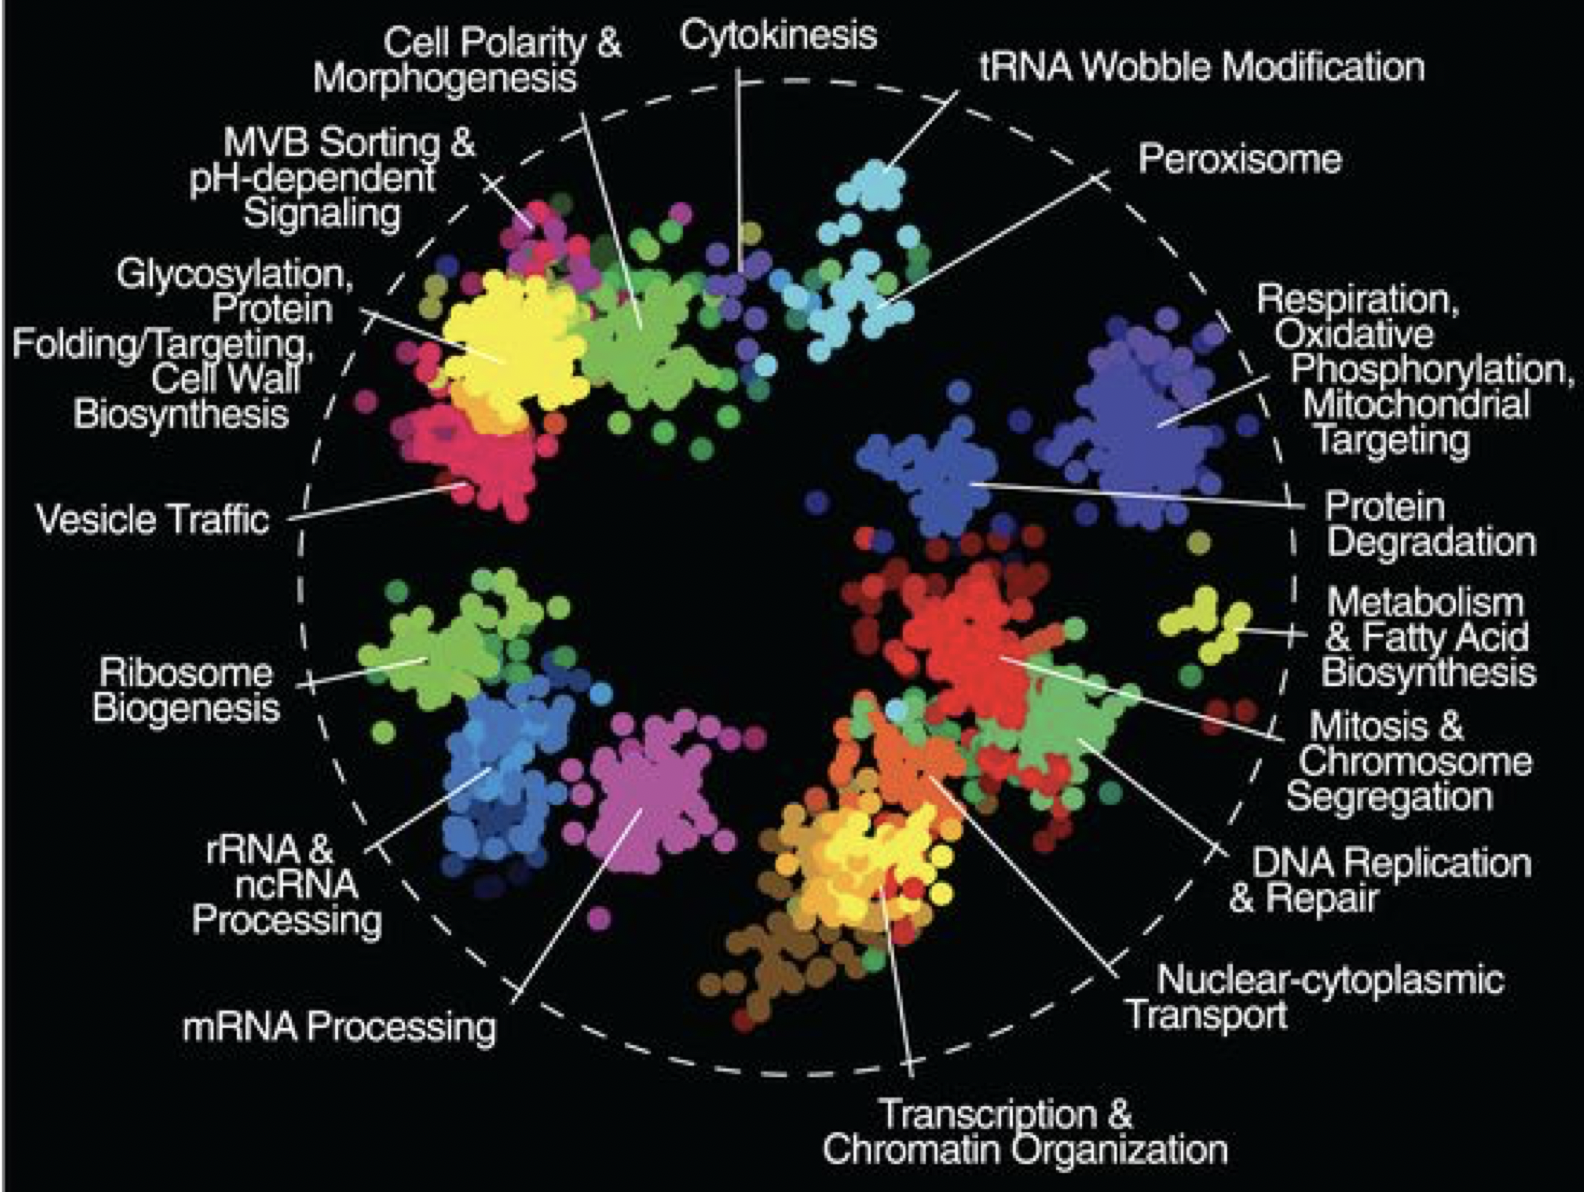
\includegraphics[width=0.75\linewidth]{slides/costanzo_functional_map.png}
  \caption{A global map of the yeast cell from genetic interaction profiles. Each dot is a gene; genes with similar genetic interaction profiles are placed near each other, and colored clusters are labelled by the biological process enriched in them. Reproduced from \citet{costanzo2016}.}
  \label{fig:costanzo}
\end{figure}

\subsection{Metabolic networks}

Metabolism is the set of chemical reactions by which a cell converts nutrients into energy and building blocks. A metabolic network has metabolites as nodes and reactions, catalyzed by enzymes, as edges; more precisely it is a bipartite graph between metabolites and reactions, or a hypergraph, since a reaction can take several substrates to several products. Pathways such as glycolysis, the citric acid cycle and fatty acid synthesis are paths through this network (Figure~\ref{fig:metabolic}). Curated metabolic pathways for many organisms are available in KEGG~\citep{kanehisa2000}.

\begin{figure}[tbp]
  \centering
  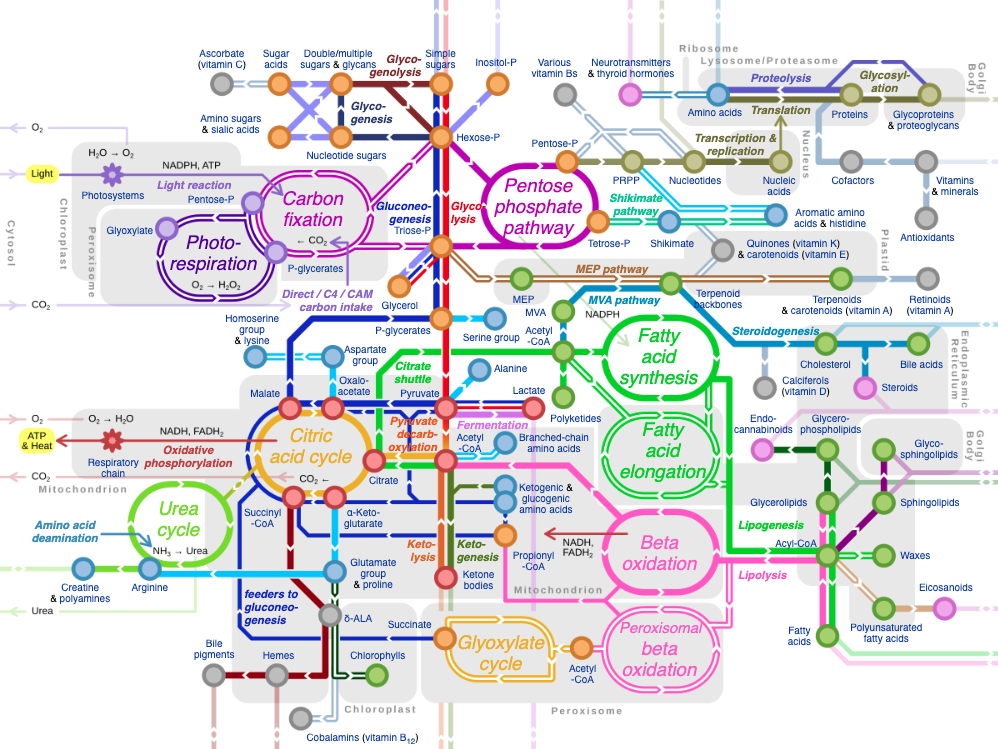
\includegraphics[width=0.8\linewidth]{slides/metabolic_metro_map.png}
  \caption{The core metabolic network drawn as a metro map. Stations are metabolites and lines are pathways. Image by Bert Chan, Hong Kong (``Metabolic Metro Map'', Wikimedia Commons).}
  \label{fig:metabolic}
\end{figure}

\subsection{Signaling networks}

Signaling networks transmit information from outside the cell to the nucleus. A ligand, such as a growth factor, binds a receptor on the cell surface, which triggers a cascade of protein modifications inside the cell, eventually changing the activity of TFs and hence gene expression (Figure~\ref{fig:signaling}). The most common modification is \emph{phosphorylation}: an enzyme called a \emph{kinase} transfers a phosphate group from ATP to a target protein, changing its shape and switching it on or off, and a \emph{phosphatase} removes the phosphate again. A cascade such as Ras$\to$Raf$\to$MEK$\to$ERK is a chain of kinases, each phosphorylating and activating the next. Signaling networks are central to cancer biology. Many oncogenes, such as \textit{RAS} and \textit{BRAF}, encode members of growth signaling pathways whose mutations make the pathway constitutively active, and many targeted cancer drugs are kinase inhibitors.

\begin{figure}[tbp]
  \centering
  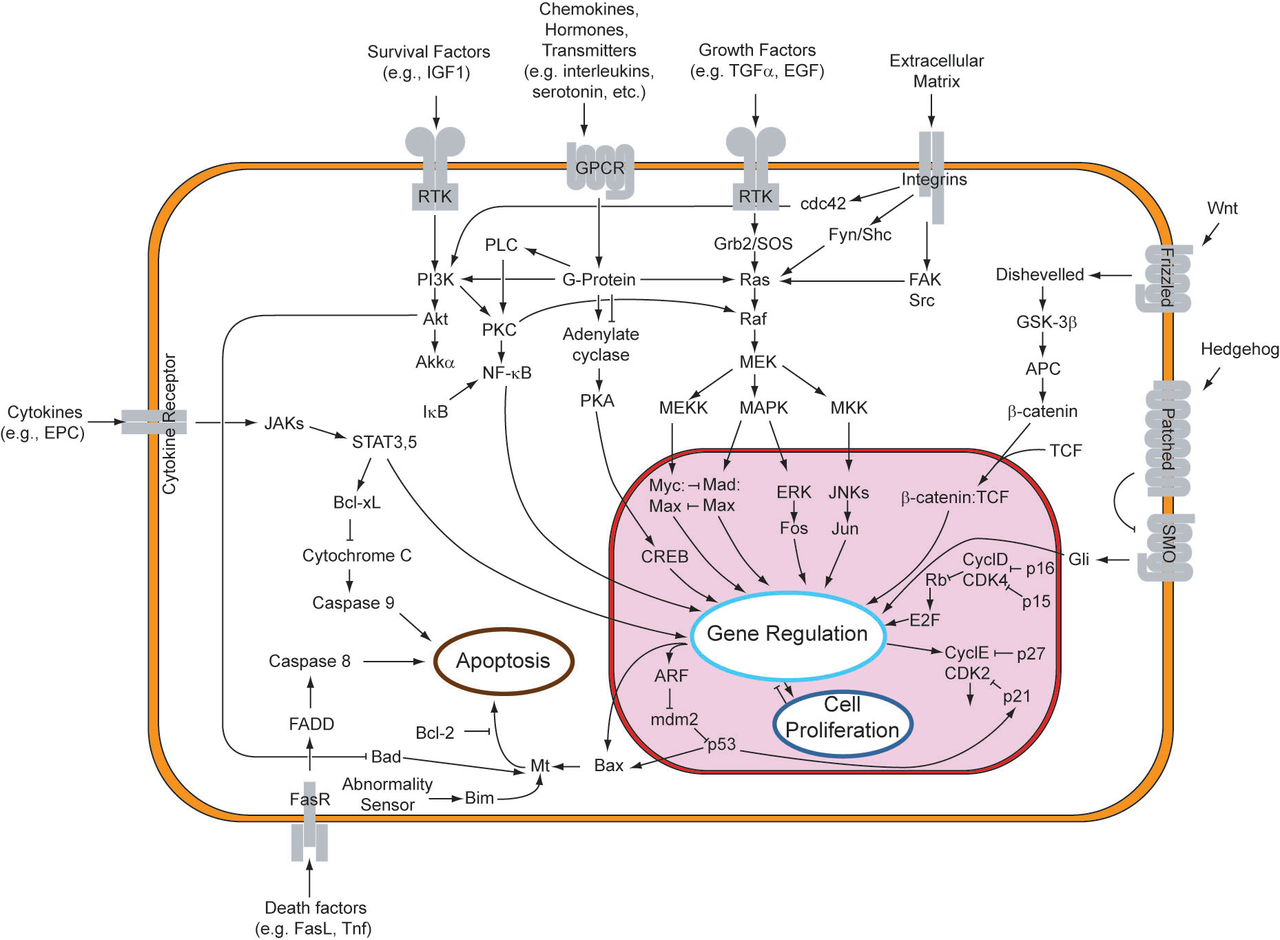
\includegraphics[width=0.85\linewidth]{slides/signaling_pathways.png}
  \caption{Major signaling pathways of a mammalian cell. Receptors at the cell membrane (orange) receive external signals such as growth factors, cytokines and death factors; cascades of protein interactions and phosphorylation in the cytoplasm relay the signal to gene regulation in the nucleus (pink), controlling proliferation and apoptosis. Source: Wikimedia Commons, signal transduction pathways diagram (source and license to be confirmed).}
  \label{fig:signaling}
\end{figure}

\subsection{Co-expression networks}

The networks above are measured, or curated from many experiments. A \emph{co-expression network} is instead inferred from expression data: nodes are genes, and an undirected edge means that the expression levels of the two genes are associated across samples. Genes regulated by the same factors will be correlated, so a co-expression network can be read as a network of co-regulation. The simplest construction connects pairs of genes whose correlation exceeds a threshold. The trouble is that correlation does not distinguish direct from indirect association. If gene $C$ regulates both $A$ and $B$, then $A$ and $B$ are correlated even though neither affects the other. The rest of the first half of this chapter develops a better approach based on partial correlation.

%======================================================================
\section{Networks of expression and splicing}
\label{sec:te_ir}
%======================================================================

Gene expression is not the only quantity a regulatory network can act on. Most human genes produce several \emph{isoforms}, transcripts that differ in which exons they include, through alternative splicing (Chapter 10). Splicing is controlled by \emph{splicing factors}, RNA-binding proteins that promote or repress the use of particular exons. \citet{saha2017} built co-expression networks from GTEx RNA-seq data~\citep{gtex2015} whose nodes are of two types. For each gene, the \emph{total expression} (TE) is the summed expression of all its isoforms. For each isoform, the \emph{isoform ratio} (IR) is its expression divided by the TE of its gene, so the IRs of a gene are non-negative and sum to one.

Table~\ref{tab:te_ir} shows why both are needed. A splicing regulator changes how a gene's transcripts are spliced. When it is abundant, most transcripts of a target gene are isoform 1; when it is scarce, more are isoform 2. The total expression of the target does not change, so a network built on TE alone cannot see this regulation, while the isoform ratios capture it.

\begin{table}[tbp]
  \centering
  \caption{Total expression (TE) and isoform ratios (IR) of a target gene with two isoforms, at high and low levels of a splicing regulator. Counts are numbers of transcripts. The regulator changes the isoform ratios but not the total expression. After an example in \citet{saha2017}.}
  \label{tab:te_ir}
  \begin{tabular}{lccccc}
    \toprule
    Splicing regulator & Isoform 1 & Isoform 2 & TE & IR$_1$ & IR$_2$ \\
    \midrule
    high & 4 & 1 & 5 & 0.8 & 0.2 \\
    low  & 2 & 3 & 5 & 0.4 & 0.6 \\
    \bottomrule
  \end{tabular}
\end{table}

The data for one tissue form a matrix $\mX\in\R^{N\times P}$, with $N$ samples (individuals) as rows and $P$ features as columns, the TE features of all genes followed by the IR features of all isoforms. The goal is a sparse undirected network over the $P$ features. The pipeline (Figure~\ref{fig:twn_pipeline}) computes the $P\times P$ sample covariance matrix, estimates a sparse inverse covariance, or precision, matrix from it with the graphical lasso, and reads the network off the non-zero entries of the precision matrix. The next two sections explain why the precision matrix is the right object and how the graphical lasso estimates it.

\begin{figure}[tbp]
  \centering
  \begin{tikzpicture}[>=Stealth, every node/.style={font=\small}]
    % data matrix
    \fill[blue!15] (0,0) rectangle (1.05,2.1);
    \fill[yellow!35] (1.05,0) rectangle (2.1,2.1);
    \draw (0,0) grid[step=0.35] (2.1,2.1);
    \node[above] at (0.525,2.1) {\footnotesize TE};
    \node[above] at (1.575,2.1) {\footnotesize IR};
    \node[left, rotate=90, anchor=south] at (-0.15,1.05) {samples ($N$)};
    \node[below] at (1.05,-0.05) {data $\mX$};
    \draw[->, thick] (2.4,1.05) -- (3.1,1.05);
    % covariance
    \begin{scope}[xshift=3.4cm]
      \fill[gray!20] (0,0) rectangle (2.1,2.1);
      \draw (0,0) grid[step=0.35] (2.1,2.1);
      \node[below, align=center] at (1.05,-0.05) {sample covariance\\$\hSigma$, $P\times P$};
    \end{scope}
    \draw[->, thick] (5.8,1.05) -- node[above, align=center] {\footnotesize graphical\\[-2pt]\footnotesize lasso} (7.1,1.05);
    % sparse precision
    \begin{scope}[xshift=7.4cm]
      \foreach \i/\j in {0/0,1/1,2/2,3/3,4/4,5/5,0/3,3/0,1/4,4/1,1/2,2/1,4/5,5/4}
        \fill[gray!45] (0.35*\i,2.1-0.35*\j-0.35) rectangle (0.35*\i+0.35,2.1-0.35*\j);
      \draw (0,0) grid[step=0.35] (2.1,2.1);
      \node[below, align=center] at (1.05,-0.05) {sparse precision\\$\hat\mTheta$, $P\times P$};
    \end{scope}
    \draw[->, thick] (9.8,1.05) -- (10.4,1.05);
    % network
    \begin{scope}[xshift=11.1cm, yshift=0.2cm, every node/.style={font=\footnotesize, inner sep=1.5pt}]
      \node[draw, circle, fill=blue!15] (t1) at (0,1.6) {1};
      \node[draw, circle, fill=blue!15] (t2) at (1.2,1.6) {2};
      \node[draw, circle, fill=blue!15] (t3) at (1.6,0.6) {3};
      \node[draw, rectangle, fill=yellow!35] (i4) at (0,0.3) {4};
      \node[draw, rectangle, fill=yellow!35] (i5) at (0.8,-0.2) {5};
      \node[draw, rectangle, fill=yellow!35] (i6) at (1.9,-0.4) {6};
      \draw (t1) -- (i4); \draw (t2) -- (i5); \draw (t2) -- (t3); \draw (i5) -- (i6);
      \node[below, font=\small] at (0.9,-0.6) {network};
    \end{scope}
  \end{tikzpicture}
  \caption{Inferring a network of total expression (TE, circles) and isoform ratio (IR, squares) features. The $N\times P$ data matrix gives a $P\times P$ sample covariance matrix; the graphical lasso estimates a sparse precision matrix whose non-zero off-diagonal entries (grey) are the edges of the network. After \citet{saha2017}.}
  \label{fig:twn_pipeline}
\end{figure}

%======================================================================
\section{Partial correlation}
\label{sec:partial_corr}
%======================================================================

\subsection{Direct and indirect association}

Consider five genes $A,B,C,D,E$. Suppose $C$ is a transcription factor that regulates both $A$ and $B$. Then $A$ and $B$ will be correlated across samples even if there is no direct relationship between them. We want an edge between $A$ and $B$ only if they remain associated after accounting for everything else that is measured. The \emph{partial correlation} of $A$ and $B$ given $C,D,E$ formalizes this. Let $x_{nA}$ be the expression of gene $A$ in sample $n$, and regress $x_A$ on the other genes,
\begin{equation}
  x_{nA} = \sum_{g\in\{C,D,E\}}\beta_gx_{ng} + \epsilon_{nA}, \qquad n=1,\dots,N.
\end{equation}
Fitting by ordinary least squares (Chapter 1) gives $\hat\vb$ and residuals $\hat\epsilon_{nA}=x_{nA}-\sum_g\hat\beta_gx_{ng}$, the part of $x_A$ that $C,D,E$ cannot explain. Doing the same for $B$ gives residuals $\hat\epsilon_{nB}$. The sample partial correlation is the correlation of the residuals,
\begin{equation}
  \cor(A,B\mid C,D,E) = \cor\left(\hat\epsilon_A,\hat\epsilon_B\right).
\end{equation}
If $C$ alone explains the association between $A$ and $B$, the residuals are uncorrelated and the partial correlation is near zero.

Running two regressions for each of the $P(P-1)/2$ pairs of genes would be expensive. It turns out that all partial correlations can be read off a single matrix, the inverse of the covariance matrix.

\subsection{Partial correlations from the precision matrix}

Let $\vx\in\R^P$ be a random vector, one sample of the expression of $P$ genes, with $\vx\sim\Normal(\mathbf{0},\mSigma)$. The data are centered so the mean is zero. $\mSigma\in\R^{P\times P}$ is the covariance matrix and $\mTheta=\mSigma^{-1}\in\R^{P\times P}$ is the \emph{precision matrix}, with entries $\theta_{ij}$. Split the coordinates into a block $1=\{A,B\}$ of size 2 and a block $2$ of the remaining $P-2$ genes, and partition
\begin{equation}
  \vx = \begin{pmatrix}\vx_1\\ \vx_2\end{pmatrix},\qquad
  \mSigma = \begin{pmatrix}\mSigma_{11} & \mSigma_{12}\\ \mSigma_{21} & \mSigma_{22}\end{pmatrix},\qquad
  \mTheta = \begin{pmatrix}\mTheta_{11} & \mTheta_{12}\\ \mTheta_{21} & \mTheta_{22}\end{pmatrix},
\end{equation}
where $\mSigma_{11},\mTheta_{11}$ are $2\times 2$, $\mSigma_{12},\mTheta_{12}$ are $2\times(P-2)$ and $\mSigma_{22},\mTheta_{22}$ are $(P-2)\times(P-2)$.

The population version of regressing $\vx_1$ on $\vx_2$ uses the coefficients that minimize expected squared error, $\mathbf{B}=\mSigma_{12}\mSigma_{22}^{-1}$, a $2\times(P-2)$ matrix. (This is the population analogue of $(\mX^\top\mX)^{-1}\mX^\top\vy$: setting the derivative of $\E\|\vx_1-\mathbf{B}\vx_2\|^2$ to zero gives $\mathbf{B}\mSigma_{22}=\mSigma_{12}$.) The residual $\veps_1=\vx_1-\mathbf{B}\vx_2$ has covariance
\begin{align}
  \Cov(\veps_1) &= \mSigma_{11} - \mathbf{B}\mSigma_{21} - \mSigma_{12}\mathbf{B}^\top + \mathbf{B}\mSigma_{22}\mathbf{B}^\top \nonumber\\
  &= \mSigma_{11} - \mSigma_{12}\mSigma_{22}^{-1}\mSigma_{21},
\end{align}
the \emph{Schur complement} of $\mSigma_{22}$ in $\mSigma$. For Gaussian $\vx$ this is also the covariance of the conditional distribution of $\vx_1$ given $\vx_2$, which is $\Normal(\mathbf{B}\vx_2,\,\mSigma_{11}-\mSigma_{12}\mSigma_{22}^{-1}\mSigma_{21})$.

The block matrix inversion formula states that the top-left block of the inverse of a partitioned matrix is the inverse of this Schur complement,
\begin{equation}
  \mTheta_{11} = \left(\mSigma_{11}-\mSigma_{12}\mSigma_{22}^{-1}\mSigma_{21}\right)^{-1}.
\end{equation}
(To check, multiply $\mSigma$ by $\mTheta$ and use $\mTheta_{21}=-\mSigma_{22}^{-1}\mSigma_{21}\mTheta_{11}$, which follows from the bottom-left block of $\mSigma\mTheta=\mI$.) So $\Cov(\veps_1)=\mTheta_{11}^{-1}$. Writing out the inverse of the $2\times2$ block,
\begin{equation}
  \mTheta_{11}^{-1} = \begin{pmatrix}\theta_{AA} & \theta_{AB}\\ \theta_{AB} & \theta_{BB}\end{pmatrix}^{-1}
  = \frac{1}{\theta_{AA}\theta_{BB}-\theta_{AB}^2}\begin{pmatrix}\theta_{BB} & -\theta_{AB}\\ -\theta_{AB} & \theta_{AA}\end{pmatrix}.
\end{equation}
The correlation of the two residuals is the off-diagonal entry divided by the square root of the product of the diagonal entries; the determinant cancels and
\begin{equation}
  \rho_{AB\mid\text{rest}} = \cor(\epsilon_A,\epsilon_B) = -\frac{\theta_{AB}}{\sqrt{\theta_{AA}\theta_{BB}}}.
  \label{eq:partial_corr}
\end{equation}
The partial correlation of every pair of variables, given all the others, is the corresponding entry of the precision matrix, rescaled by the diagonal and with its sign flipped. In particular, $\rho_{AB\mid\text{rest}}=0$ exactly when $\theta_{AB}=0$.

The same block formula with block $1=\{A\}$ alone relates the precision matrix to the regression of one gene on all the others. Using $\mTheta_{21}=-\mSigma_{22}^{-1}\mSigma_{21}\mTheta_{11}$ with $\mTheta_{11}=\theta_{AA}$ a scalar, the regression coefficients are $\mSigma_{22}^{-1}\mSigma_{21}=-\mTheta_{21}/\theta_{AA}$, that is
\begin{equation}
  \beta_{Aj} = -\frac{\theta_{Aj}}{\theta_{AA}}, \qquad \Var(\epsilon_A) = \frac{1}{\theta_{AA}}.
\end{equation}
Gene $j$ has a non-zero coefficient in the regression of $A$ on all other genes exactly when $\theta_{Aj}\neq 0$. This suggests estimating the network by a sparse (lasso) regression of each gene on all the others, \emph{neighbourhood selection}~\citep{meinshausen2006}.

\subsection{Conditional independence and Gaussian graphical models}

For Gaussian $\vx$, the conditional distribution of $(x_A,x_B)$ given the other genes is Gaussian with covariance $\mTheta_{11}^{-1}$. A bivariate Gaussian has independent components if and only if its covariance is diagonal, so
\begin{equation}
  \rho_{AB\mid\text{rest}}=0 \iff \theta_{AB}=0 \iff x_A\indep x_B\mid \vx_{\text{rest}} .
\end{equation}
The same conclusion follows from the density. Up to a constant, $\log p(\vx) = \frac12\log|\mTheta| - \frac12\sum_{i,j}\theta_{ij}x_ix_j$, so if $\theta_{AB}=0$ no term couples $x_A$ and $x_B$ and the density factorizes into a part involving $x_A$ and a part involving $x_B$, given the rest. A Gaussian distribution together with the graph whose edges are the non-zero off-diagonal entries of $\mTheta$ is a \emph{Gaussian graphical model}, or Gaussian Markov random field. Missing edges are conditional independences. The equivalence between zero partial correlation and conditional independence is special to the Gaussian; for other distributions zero partial correlation only means the absence of linear association given the other variables.

The precision matrix contains the direct associations; the covariance matrix contains direct and indirect associations mixed together. In the five-gene example above, if $A$ is directly linked only to $C$ and $B$ only to $E$, then $\theta_{AB}=0$ and the graph has no $A$--$B$ edge, though $\Sigma_{AB}$ may be far from zero if $C$ and $E$ are themselves associated.

Figure~\ref{fig:partial_corr} illustrates this with a simulated network of eight genes: a hub (gene 1 linked to genes 2, 3 and 4), a chain $5-6-7$, and an isolated gene 8. The sample correlation matrix is dense, because genes 2, 3 and 4 are correlated through gene 1 and genes 5 and 7 through gene 6. With $N=100$ samples genes 5 and 7 have sample correlation $\corrFiveSeven$ but sample partial correlation $\pcorFiveSeven$. The partial correlations computed from the inverse of the sample covariance recover the structure, but with noise everywhere; the graphical lasso (Section~\ref{sec:glasso}) sets most of the spurious entries exactly to zero.

\begin{figure}[tbp]
  \centering
  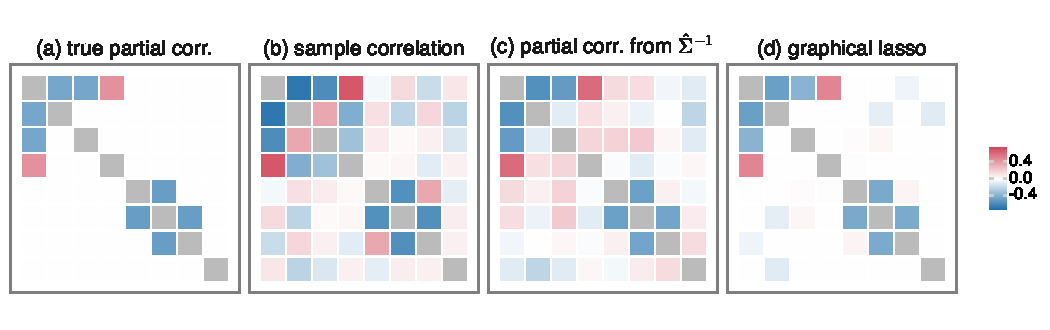
\includegraphics[width=\linewidth]{partial_correlation.pdf}
  \caption{Correlation and partial correlation for eight simulated genes ($N=100$ samples). (a) True partial correlations $-\theta_{ij}/\sqrt{\theta_{ii}\theta_{jj}}$: gene 1 is a hub linked to genes 2--4 and genes 5--6--7 form a chain. (b) The sample correlation matrix is dense, because of indirect associations. (c) Partial correlations from the inverse sample covariance $\hSigma^{-1}$ recover the structure, with noise. (d) Partial correlations from the graphical lasso with $\lambda=0.1$, which are exactly zero for most non-edges. Diagonal entries are grey.}
  \label{fig:partial_corr}
\end{figure}

%======================================================================
\section{The graphical lasso}
\label{sec:glasso}
%======================================================================

\subsection{Gaussian likelihood in terms of the precision matrix}

Let $\vx_n\in\R^P$, $n=1,\dots,N$, be the centered expression vectors of $N$ samples, assumed independent and identically distributed as $\vx_n\sim\Normal(\mathbf{0},\mTheta^{-1})$ with unknown $P\times P$ precision matrix $\mTheta$. The Gaussian density is $p(\vx_n)=(2\pi)^{-P/2}|\mTheta|^{1/2}\exp(-\frac12\vx_n^\top\mTheta\vx_n)$, using $|\mSigma|^{-1/2}=|\mTheta^{-1}|^{-1/2}=|\mTheta|^{1/2}$. The log likelihood is
\begin{equation}
  \log L(\mTheta) = \sum_{n=1}^N\left(\frac12\log|\mTheta| - \frac12\vx_n^\top\mTheta\vx_n\right) + \text{const}.
\end{equation}
A scalar equals its own trace, and the trace is invariant to cyclic permutations, so $\vx_n^\top\mTheta\vx_n=\tr(\vx_n^\top\mTheta\vx_n)=\tr(\mTheta\vx_n\vx_n^\top)$. Summing over $n$ and using linearity of the trace,
\begin{equation}
  \sum_{n=1}^N\vx_n^\top\mTheta\vx_n = \tr\Big(\mTheta\sum_{n=1}^N\vx_n\vx_n^\top\Big) = N\tr(\mTheta\hSigma),
  \qquad \hSigma = \frac1N\sum_{n=1}^N\vx_n\vx_n^\top = \frac1N\mX^\top\mX,
\end{equation}
where $\hSigma\in\R^{P\times P}$ is the sample covariance matrix. Therefore
\begin{equation}
  \log L(\mTheta) = \frac N2\left(\log|\mTheta| - \tr(\mTheta\hSigma)\right) + \text{const}.
  \label{eq:gauss_loglik}
\end{equation}
The data enter only through $\hSigma$, a sufficient statistic.

To maximize, we need two matrix derivatives: $\partial\log|\mTheta|/\partial\mTheta=\mTheta^{-1}$ for symmetric positive definite $\mTheta$, and $\partial\tr(\mTheta\hSigma)/\partial\mTheta=\hSigma$. Setting the gradient of~\eqref{eq:gauss_loglik} to zero gives $\mTheta^{-1}=\hSigma$, so the maximum likelihood estimate is $\hat\mTheta=\hSigma^{-1}$, as used in Figure~\ref{fig:partial_corr}c. This estimate has two problems for genomic data. First, $\hSigma=\frac1N\mX^\top\mX$ has rank at most $N$ (at most $N-1$ once the data are centered), so when $N\le P$ it is singular and the inverse does not exist; with $P=10{,}000$ genes we would need more than 10{,}000 samples. Second, even when $N>P$, $\hSigma^{-1}$ is noisy and dense: no entry is exactly zero, so it does not give a network.

\subsection{The L1-penalized objective}

The graphical lasso~\citep{friedman2008,yuan2007,banerjee2008} applies the idea of the lasso (Chapter 1) to the precision matrix. Multiplying the log likelihood~\eqref{eq:gauss_loglik} by $-2/N$ to obtain a loss, and adding an L1 penalty on the entries of $\mTheta$,
\begin{equation}
  \hat\mTheta = \argmin_{\mTheta\succ 0}\; -\log|\mTheta| + \tr(\mTheta\hSigma) + \lambda\|\mTheta\|_1,
  \qquad \|\mTheta\|_1=\sum_{i,j}|\theta_{ij}|,
  \label{eq:glasso}
\end{equation}
where $\mTheta\succ0$ restricts $\mTheta$ to symmetric positive definite matrices and $\lambda\ge0$ is the regularization strength. Many implementations penalize only the off-diagonal entries, since the diagonal is always non-zero and does not correspond to edges. As in the lasso, the L1 penalty sets many entries of $\hat\mTheta$ exactly to zero, giving a sparse network, and for $\lambda>0$ the solution exists even when $\hSigma$ is singular.

The problem is convex. The function $-\log|\mTheta|$ is convex on positive definite matrices, $\tr(\mTheta\hSigma)$ is linear and $\|\mTheta\|_1$ is convex, so any local minimum is the global minimum. Whatever initialization or algorithm is used, a correct solver arrives at the same answer, unlike many of the non-convex problems in this book.

\subsection{A block coordinate descent algorithm}

The minimizer of~\eqref{eq:glasso} satisfies the subgradient condition
\begin{equation}
  \mTheta^{-1} - \hSigma - \lambda\mGamma = \mathbf{0},
  \label{eq:glasso_kkt}
\end{equation}
where $\mGamma$ is a $P\times P$ matrix with $\gamma_{ij}=\operatorname{sign}(\theta_{ij})$ if $\theta_{ij}\neq0$ and $\gamma_{ij}\in[-1,1]$ if $\theta_{ij}=0$. Let $\mathbf{W}=\mTheta^{-1}$ be the current estimate of the covariance. Condition~\eqref{eq:glasso_kkt} says $|w_{ij}-\hat\sigma_{ij}|\le\lambda$, with equality wherever $\theta_{ij}\neq0$: the estimated covariance may differ from the sample covariance by at most $\lambda$ in each entry.

\citet{friedman2008} solve~\eqref{eq:glasso_kkt} one row and column at a time. Partition $\mathbf{W}$, $\hSigma$, $\mTheta$ and $\mGamma$ with the last row and column separated, for example
\begin{equation}
  \mathbf{W} = \begin{pmatrix}\mathbf{W}_{11} & \mathbf{w}_{12}\\ \mathbf{w}_{12}^\top & w_{22}\end{pmatrix},
\end{equation}
where $\mathbf{W}_{11}$ is $(P-1)\times(P-1)$, $\mathbf{w}_{12}\in\R^{P-1}$ and $w_{22}$ is a scalar. The upper-right block of~\eqref{eq:glasso_kkt} is $\mathbf{w}_{12}-\hat{\boldsymbol\sigma}_{12}-\lambda\boldsymbol\gamma_{12}=\mathbf{0}$. The upper-right block of $\mathbf{W}\mTheta=\mI$ is $\mathbf{W}_{11}\boldsymbol\theta_{12}+\mathbf{w}_{12}\theta_{22}=\mathbf{0}$, so $\mathbf{w}_{12}=\mathbf{W}_{11}\vb$ with $\vb=-\boldsymbol\theta_{12}/\theta_{22}\in\R^{P-1}$. Because $\theta_{22}>0$, $\vb$ and $\boldsymbol\theta_{12}$ have opposite signs and the same zeros, so $\boldsymbol\gamma_{12}=-\boldsymbol\nu$ with $\nu_j\in\operatorname{sign}(\beta_j)$. Substituting,
\begin{equation}
  \mathbf{W}_{11}\vb - \hat{\boldsymbol\sigma}_{12} + \lambda\boldsymbol\nu = \mathbf{0}.
\end{equation}
This is the subgradient condition of
\begin{equation}
  \min_{\vb}\;\frac12\vb^\top\mathbf{W}_{11}\vb - \vb^\top\hat{\boldsymbol\sigma}_{12} + \lambda\|\vb\|_1,
\end{equation}
which is a lasso regression: with $\mathbf{W}_{11}=\hSigma_{11}$ it is exactly the lasso regression of the last variable on the others, written in terms of the covariances $\mX^\top\mX/N$ and $\mX^\top\vy/N$. It can be solved by coordinate descent, cycling over $j$ and updating
\begin{equation}
  \beta_j \leftarrow \frac{\mathcal{S}\big(\hat\sigma_{12,j}-\sum_{k\neq j}(\mathbf{W}_{11})_{kj}\beta_k,\;\lambda\big)}{(\mathbf{W}_{11})_{jj}},
\end{equation}
where $\mathcal{S}(u,\lambda)=\operatorname{sign}(u)\max(|u|-\lambda,0)$ is the soft-thresholding operator from Chapter 1. The algorithm initializes $\mathbf{W}=\hSigma+\lambda\mI$ (the diagonal of~\eqref{eq:glasso_kkt} when the diagonal is penalized), then cycles over the columns: each column in turn is moved to the last position, its lasso problem solved, and $\mathbf{w}_{12}=\mathbf{W}_{11}\hat\vb$ filled in. On convergence, $\mTheta$ is recovered from $\theta_{22}=1/(w_{22}-\mathbf{w}_{12}^\top\hat\vb)$ and $\boldsymbol\theta_{12}=-\hat\vb\,\theta_{22}$. Each column's lasso is the neighbourhood regression of the previous section, coupled across columns through $\mathbf{W}$. \citet{mazumder2012} analyze this algorithm and alternatives, including solving the primal problem directly; proximal gradient methods also work.

\subsection{\texorpdfstring{Choosing $\lambda$}{Choosing lambda}}

As in regression, $\lambda$ trades off fit and sparsity. Cross-validation applies even though there is no response variable: the Gaussian model assigns a likelihood to held-out samples. For each fold, fit $\hat\mTheta$ on the training samples and evaluate~\eqref{eq:gauss_loglik} with $\hat\mTheta$ and the held-out sample covariance. Figure~\ref{fig:glasso_path} shows the regularization path and the cross-validated log likelihood for $P=40$ simulated genes with 25 true edges and only $N=30$ samples, so that $\hSigma$ has rank $\pathRank$ and cannot be inverted. Small $\lambda$ overfits and gives a poor held-out likelihood. The cross-validated optimum, $\lambda=\pathBestLambda$, keeps $\pathBestEdges$ edges, $\pathBestTrue$ of them true. Cross-validation optimizes prediction, and the predictive optimum typically includes some false positive edges; if the network itself is the goal, a larger $\lambda$ or a stability-based criterion may be preferable.

\begin{figure}[tbp]
  \centering
  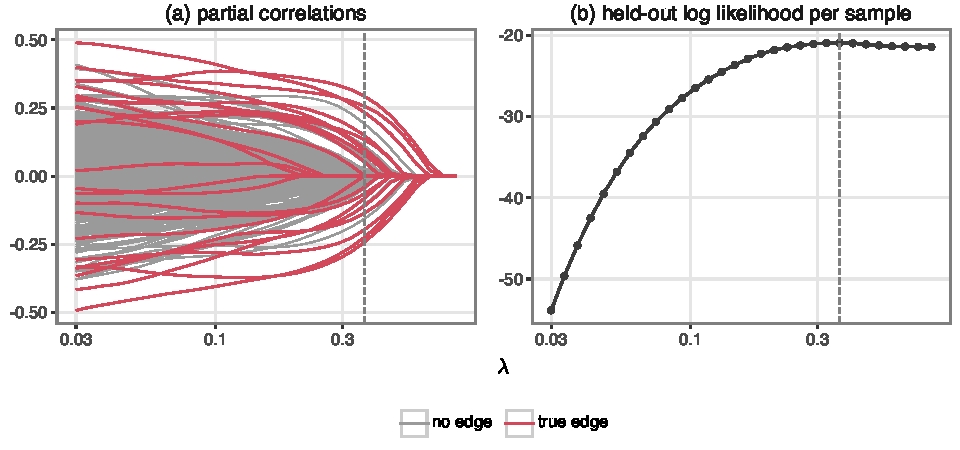
\includegraphics[width=0.95\linewidth]{glasso_path.pdf}
  \caption{The graphical lasso on simulated data with $P=40$ genes, 25 true edges and $N=30$ samples. (a) Partial correlations as a function of $\lambda$, for true edges (red) and non-edges (grey); every partial correlation reaches zero for large enough $\lambda$, and true edges tend to persist longest. (b) Five-fold cross-validated Gaussian log likelihood per held-out sample. The dashed line marks the $\lambda$ that maximizes it.}
  \label{fig:glasso_path}
\end{figure}

\subsection{Using the graphical lasso on expression data}

Several practical points matter when applying the graphical lasso to gene expression.
\begin{itemize}
  \item The model is Gaussian. Count data should be normalized and log-transformed, or each gene's values replaced by Gaussian quantiles of its ranks, an approach formalized by the nonparanormal~\citep{liu2009}.
  \item Hidden confounders, such as batch, RNA quality or cell-type composition, affect many genes at once and induce dense correlations. They are commonly removed first by regressing out known covariates and leading principal components or factors (Chapter 8).
  \item The network is undirected. An edge means a conditional association, not a causal or regulatory direction.
  \item Penalties need not be equal. With TE and IR features, for example, one could use different values of $\lambda$ for TE--TE, TE--IR and IR--IR entries. The isoform ratios of a gene sum to one, so one of them is a linear function of the others; dropping one ratio per gene avoids an exactly singular covariance.
\end{itemize}

\subsection{Network motifs}

Recurring local patterns in a network are called \emph{network motifs}, a term borrowed from the sequence motifs bound by TFs. In a network of TE and IR features, a node connected to many others is a \emph{hub}, and the type of hub suggests a mechanism (Figure~\ref{fig:hubs}). A TE node linked to many TE nodes could be a TF that regulates the expression of many targets. A TE node linked to many IR nodes could be a splicing factor, whose expression level controls the splicing of many targets. An IR node of a gene linked to many TE nodes suggests a TF with several isoforms that differ in their regulatory activity. An IR node linked to many IR nodes suggests alternative splicing of a splicing factor. Splicing factors often regulate the splicing of their own transcripts, a form of autoregulation that complicates the interpretation of such networks.

\begin{figure}[tbp]
  \centering
  \begin{tikzpicture}[every node/.style={font=\footnotesize},
      te/.style={draw, ellipse, fill=blue!15, minimum width=0.75cm, minimum height=0.45cm, inner sep=1pt},
      ir/.style={draw, rectangle, rounded corners=1pt, fill=yellow!35, minimum width=0.6cm, minimum height=0.45cm, inner sep=1pt}]
    \foreach \hx/\htype/\ltype/\lab/\mech in {0/te/te/TE--TE hub/{TF?}, 3.4/te/ir/TE--IR hub/{splicing factor}, 6.8/ir/te/IR--TE hub/{alternative splicing\\of a TF}, 10.2/ir/ir/IR--IR hub/{alternative splicing\\of a splicing factor}} {
      \node[\htype, thick] (h) at (\hx,0) {hub};
      \foreach \a in {90,162,234,306,18} {
        \node[\ltype] (l\a) at ($(\hx,0)+(\a:1.15)$) {};
        \draw (h) -- (l\a);
      }
      \node[below, font=\small] at (\hx,-1.45) {\lab};
      \node[below, align=center] at (\hx,-1.85) {\mech};
    }
  \end{tikzpicture}
  \caption{Four kinds of hub in a network of total expression (TE, ellipses) and isoform ratio (IR, rectangles) features, and the mechanism each suggests. After \citet{saha2017}.}
  \label{fig:hubs}
\end{figure}

%======================================================================
\section{Tissue-specific networks}
\label{sec:gtex}
%======================================================================

\subsection{The GTEx project}

The Genotype-Tissue Expression (GTEx) project~\citep{gtex2013,gtex2015,gtex2020} collected many tissues from postmortem donors, eventually close to a thousand individuals and around 50 tissues, and measured gene expression in each by RNA-seq and the donors' genotypes by sequencing or genotyping arrays. Its main aim was mapping genetic variants that affect expression (Chapter 12), but it is also a resource for asking how gene networks differ between tissues. Different tissues express different genes and are regulated differently, so a network estimated from one tissue need not hold in another.

Sample sizes per tissue are modest. In the early releases most tissues had tens of samples and the best represented, such as whole blood and skeletal muscle, had one to two hundred. Estimating a $10{,}000\times10{,}000$ precision matrix from 168 blood samples, for example, is a very high-dimensional problem. Some tissues are similar to each other, however. GTEx sampled more than ten brain regions, which in retrospect have similar expression profiles; arteries from different sites resemble each other, as do stomach and colon. Hierarchical clustering (Chapter 5) of the tissues' average expression profiles makes these similarities explicit (Figure~\ref{fig:gtex_dendrogram}). Information can therefore be shared between related tissues when estimating their networks. Pooling samples from similar tissues is the crude version of this; \citet{pierson2015} proposed a more principled one. Figure~\ref{fig:coronary} shows part of a network they inferred for coronary artery.

\begin{figure}[tbp]
  \centering
  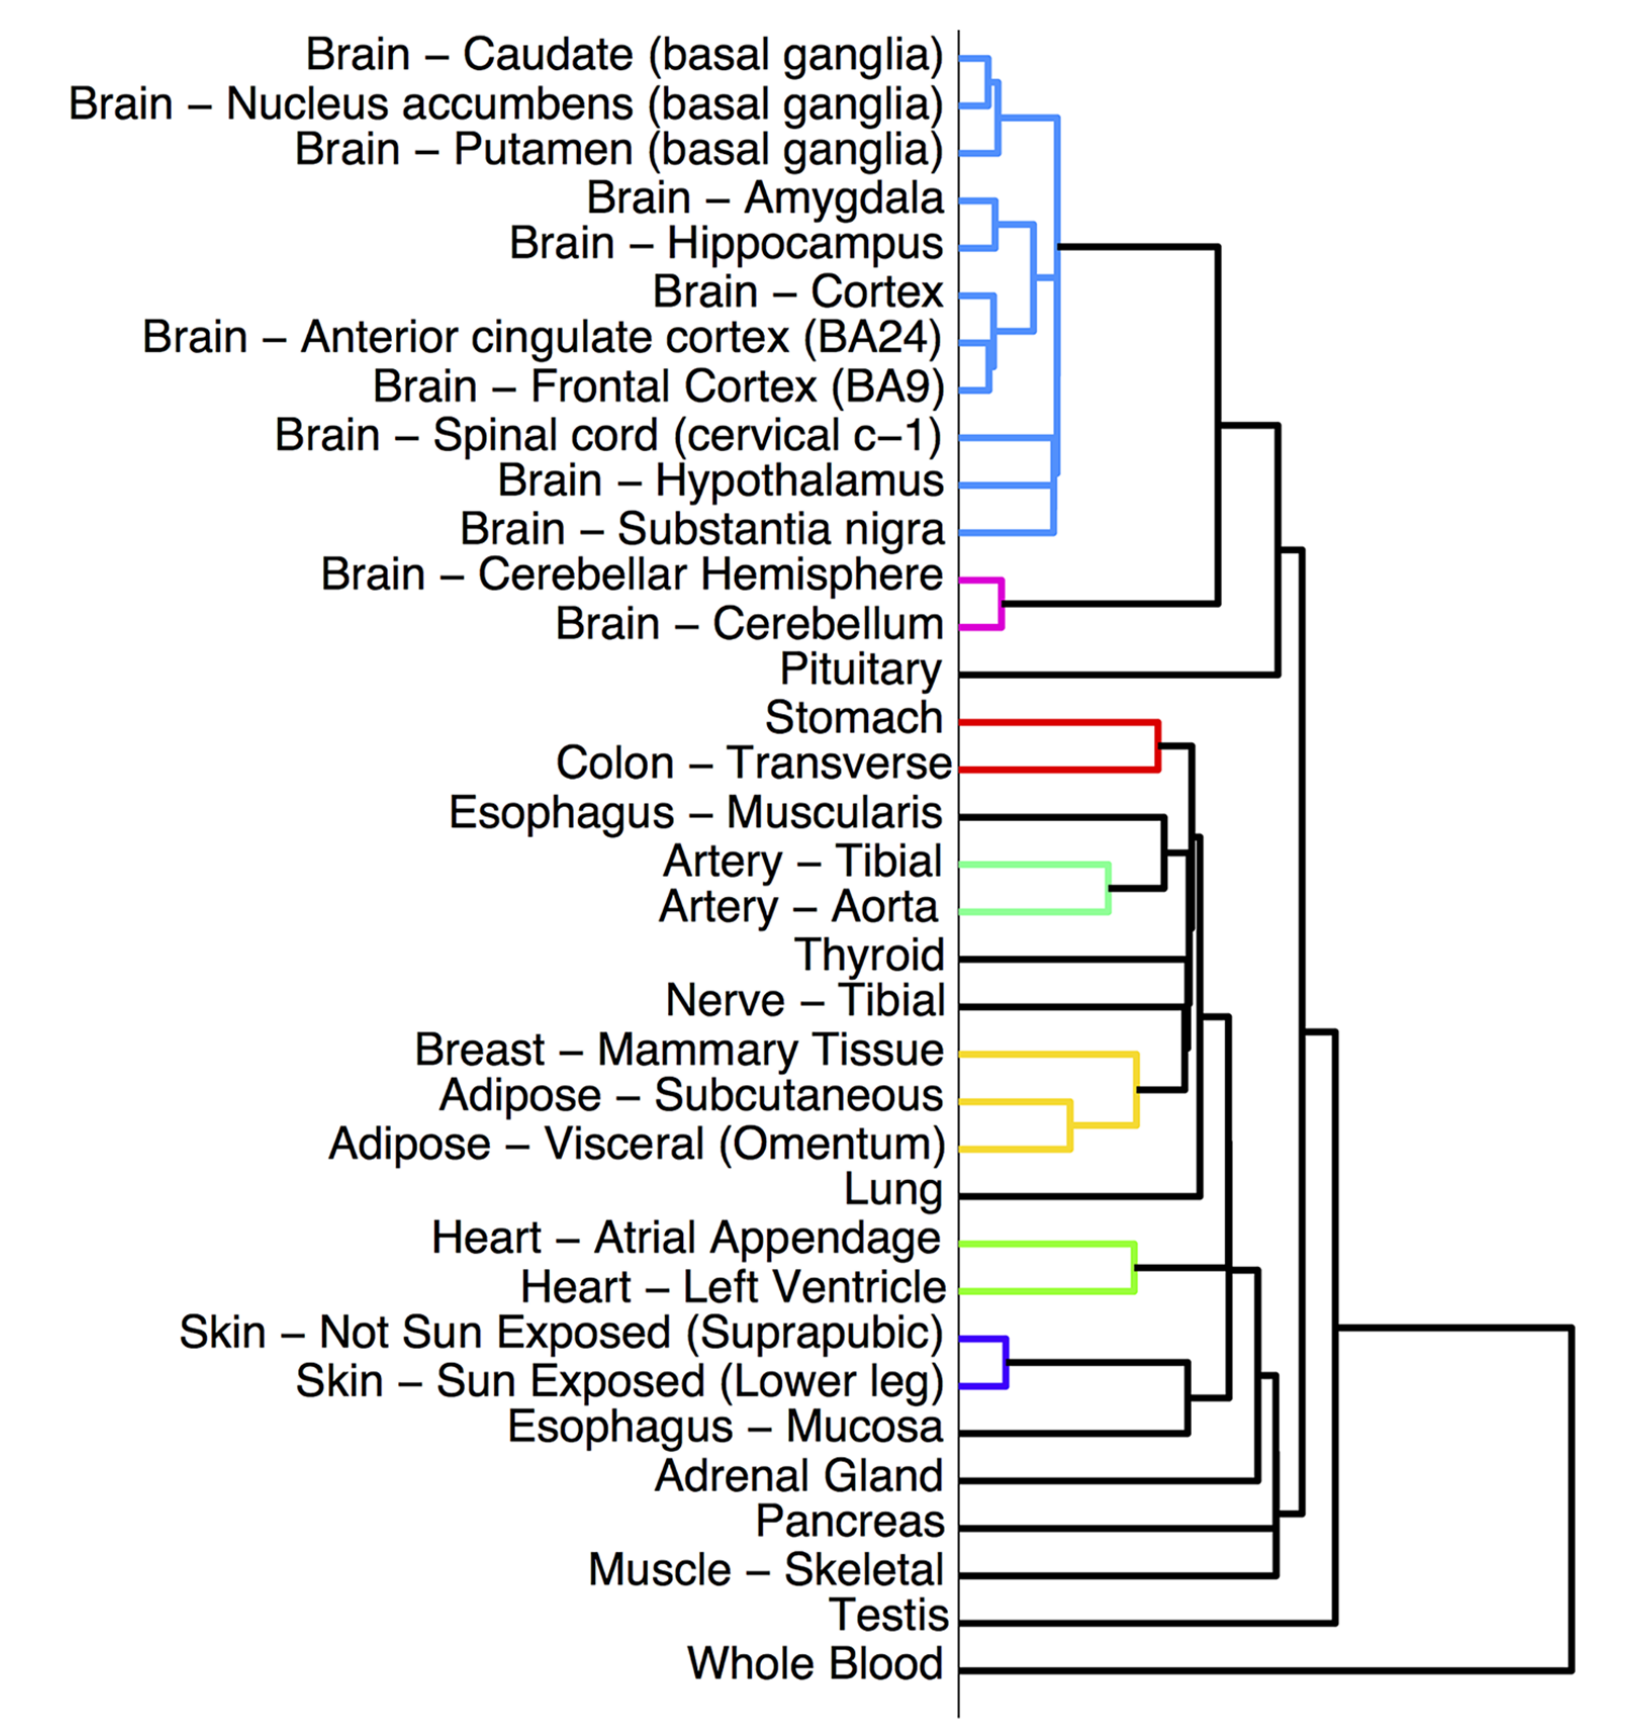
\includegraphics[width=0.6\linewidth]{slides/gtex_tissue_dendrogram.png}
  \caption{Hierarchical clustering of GTEx tissues by their average expression profiles. Brain regions form one tight cluster; arteries, the two adipose depots, the two heart samples and the two skin samples each cluster together. Reproduced from \citet{pierson2015}.}
  \label{fig:gtex_dendrogram}
\end{figure}

\begin{figure}[tbp]
  \centering
  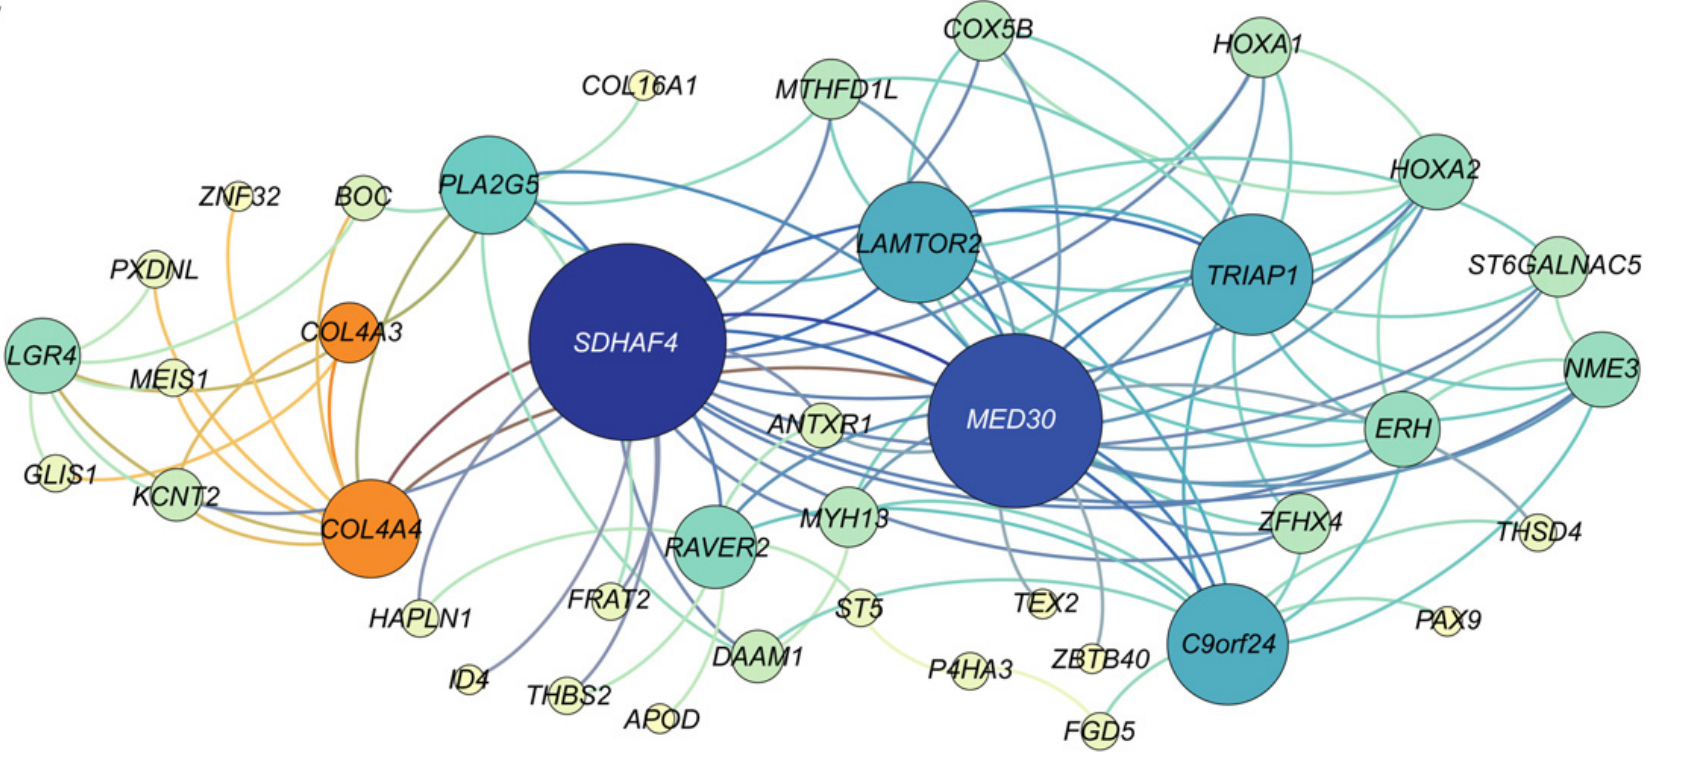
\includegraphics[width=0.8\linewidth]{slides/pierson_coronary_network.png}
  \caption{Part of a co-expression network inferred for GTEx coronary artery. Node size reflects the number of connections. Reproduced from \citet{pierson2015}.}
  \label{fig:coronary}
\end{figure}

\subsection{Sharing networks along a tissue hierarchy}

Let there be $K$ tissues, with $n^{(k)}$ samples and sample covariance $\hSigma^{(k)}\in\R^{P\times P}$ for tissue $k$. The tissue tree from hierarchical clustering is a rooted binary tree with the $K$ observed tissues as leaves, numbered $1,\dots,K$. A rooted binary tree with $K$ leaves has $K-1$ internal nodes, numbered $K+1,\dots,2K-1$ with the root last, and $2K-2$ edges, since every node except the root has exactly one parent. Each internal node can be thought of as an unobserved ``ancestral'' tissue. Give every node $k$ of the tree, leaf or internal, a precision matrix $\mTheta^{(k)}\in\R^{P\times P}$, and let $p(k)$ denote the parent of node $k$. \citet{pierson2015} estimate all $2K-1$ matrices jointly by maximizing
\begin{equation}
  \sum_{k=1}^{K}\frac{n^{(k)}}{2}\left(\log|\mTheta^{(k)}| - \tr\big(\mTheta^{(k)}\hSigma^{(k)}\big) - \lambda_s^{(k)}\|\mTheta^{(k)}\|_1\right)
  - \lambda_p\sum_{k=1}^{2K-2}\big\|\mTheta^{(k)}-\mTheta^{(p(k))}\big\|_2^2 ,
  \label{eq:gtex_objective}
\end{equation}
where $\|\cdot\|_2^2$ is the squared Frobenius norm, the sum of squared entries. The first sum is a graphical lasso objective for each observed tissue, weighted by its sample size, with tissue-specific sparsity penalties $\lambda_s^{(k)}$. The second sum runs over the $2K-2$ edges of the tree and penalizes the squared difference between the precision matrix of each node and that of its parent, with strength $\lambda_p\ge0$. With $\lambda_p=0$ the tissues are estimated independently. As $\lambda_p\to\infty$ all nodes are forced to share one network, which amounts to pooling. In between, each tissue's network is pulled toward those of the tissues near it in the tree. For a tree with $K=3$ leaves in which tissues 1 and 2 share parent 4, and 4 and 3 are children of the root 5, the four penalty terms are $\|\mTheta^{(1)}-\mTheta^{(4)}\|^2$, $\|\mTheta^{(2)}-\mTheta^{(4)}\|^2$, $\|\mTheta^{(4)}-\mTheta^{(5)}\|^2$ and $\|\mTheta^{(3)}-\mTheta^{(5)}\|^2$.

Figure~\ref{fig:tissue_tree} gives the intuition with three genes. Estimated separately, each tissue's network reflects its own small sample. An internal node's network is an average of its children: if both children have an $A$--$B$ edge, so does the parent, and if only one has an $A$--$C$ edge, the parent has a weaker one. Re-estimating each tissue with a pull toward its parent then shares edges between similar tissues.

\begin{figure}[tbp]
  \centering
  \begin{tikzpicture}[every node/.style={font=\scriptsize}]
    \newcommand{\abc}[6]{% x, y, color, A-B width, A-C width, B-C width (0pt = no edge)
      \begin{scope}[shift={(#1,#2)}]
        \node[draw, circle, fill=#3, inner sep=1pt, minimum size=0.36cm] (nA) at (-0.3,0) {A};
        \node[draw, circle, fill=#3, inner sep=1pt, minimum size=0.36cm] (nB) at (0.3,0) {B};
        \node[draw, circle, fill=#3, inner sep=1pt, minimum size=0.36cm] (nC) at (0,-0.5) {C};
        \ifdim#4>0pt \draw[line width=#4] (nA) -- (nB); \fi
        \ifdim#5>0pt \draw[line width=#5] (nA) -- (nC); \fi
        \ifdim#6>0pt \draw[line width=#6] (nB) -- (nC); \fi
      \end{scope}}
    \foreach \sx/\lab in {0/{(a) separate estimates}, 7.2/{(b) shared along the tree}} {
      \begin{scope}[xshift=\sx cm]
        \draw[thick, gray] (0,0.35) -- (0,1.0) -- (1.6,1.0) -- (1.6,0.35);
        \draw[thick, gray] (3.2,0.35) -- (3.2,1.0) -- (4.8,1.0) -- (4.8,0.35);
        \draw[thick, gray] (0.8,1.0) -- (0.8,2.1) -- (4.0,2.1) -- (4.0,1.0);
        \node[font=\small] at (2.4,-1.1) {\lab};
      \end{scope}
    }
    % (a) leaves only
    \abc{0}{0}{green!35}{1.4pt}{0pt}{0pt}
    \abc{1.6}{0}{green!35}{1.4pt}{1.4pt}{0pt}
    \abc{3.2}{0}{red!35}{1.4pt}{0pt}{1.4pt}
    \abc{4.8}{0}{red!35}{0pt}{0pt}{0pt}
    % (b) leaves, parents and root
    \abc{7.2}{0}{green!35}{1.4pt}{0.8pt}{0pt}
    \abc{8.8}{0}{green!35}{1.4pt}{1.2pt}{0pt}
    \abc{10.4}{0}{red!35}{1.2pt}{0pt}{1.4pt}
    \abc{12.0}{0}{red!35}{1.0pt}{0pt}{1.2pt}
    \abc{8.0}{1.7}{green!12}{1.4pt}{0.8pt}{0pt}
    \abc{11.2}{1.7}{red!12}{1.0pt}{0pt}{1.0pt}
    \abc{9.6}{2.85}{white}{1.2pt}{0.4pt}{0.4pt}
  \end{tikzpicture}
  \caption{Sharing networks between related tissues, with three genes $A,B,C$. Two related tissues are green and two are red; the grey tree is the tissue hierarchy. (a) Networks estimated separately for each tissue. (b) Internal nodes carry networks that average their neighbours, and each tissue's network is pulled toward its parent's, so that edges are shared between similar tissues. Line width indicates edge strength. After \citet{pierson2015}.}
  \label{fig:tissue_tree}
\end{figure}

\subsection{Optimization}

Objective~\eqref{eq:gtex_objective} is concave (its negative is convex), and it is maximized by alternating between the two kinds of node.
\begin{enumerate}
  \item \emph{Leaves.} With the internal nodes fixed, the objective separates over tissues. Leaf $k$ appears in its graphical lasso term and in one penalty term, the edge to its parent, so its update is
  \begin{equation}
    \hat\mTheta^{(k)} = \argmax_{\mTheta\succ0}\;\frac{n^{(k)}}{2}\left(\log|\mTheta|-\tr\big(\mTheta\hSigma^{(k)}\big)-\lambda_s^{(k)}\|\mTheta\|_1\right) - \lambda_p\big\|\mTheta-\mTheta^{(p(k))}\big\|_2^2,
  \end{equation}
  a graphical lasso with an extra quadratic term pulling $\mTheta$ toward the parent. It can be solved with the same tools as the graphical lasso, for example proximal gradient methods.
  \item \emph{Internal nodes.} With the leaves fixed, the internal nodes appear only in the penalty, which is quadratic. Differentiating with respect to internal node $m$, which appears in the terms for its two children and, unless it is the root, its parent, and setting the result to zero,
  \begin{equation}
    \sum_{k\in\mathcal{N}(m)}2\lambda_p\left(\mTheta^{(m)}-\mTheta^{(k)}\right)=\mathbf{0}
    \quad\Longrightarrow\quad
    \mTheta^{(m)} = \frac{1}{|\mathcal{N}(m)|}\sum_{k\in\mathcal{N}(m)}\mTheta^{(k)},
  \end{equation}
  where $\mathcal{N}(m)$ is the set of tree neighbours of $m$ (two children and a parent, or two children for the root). At the optimum each internal node is the average of its neighbours. These conditions for all internal nodes form a linear system, the graph Laplacian of the tree restricted to its internal nodes, that is solved once for all entries of the matrices. The solution expresses each internal matrix as a weighted average of the leaf matrices with non-negative weights summing to one, so the internal matrices are positive definite whenever the leaves are.
\end{enumerate}

\subsection{Evaluation and interpretation}

As in Figure~\ref{fig:glasso_path}b, the model is evaluated by the cross-validated Gaussian likelihood of held-out samples. Figure~\ref{fig:pierson_cv} shows the improvement over estimating each tissue separately ($\lambda_p=0$) as $\lambda_p$ increases, for three gene sets. Sharing across the hierarchy improves the held-out likelihood substantially.

\begin{figure}[tbp]
  \centering
  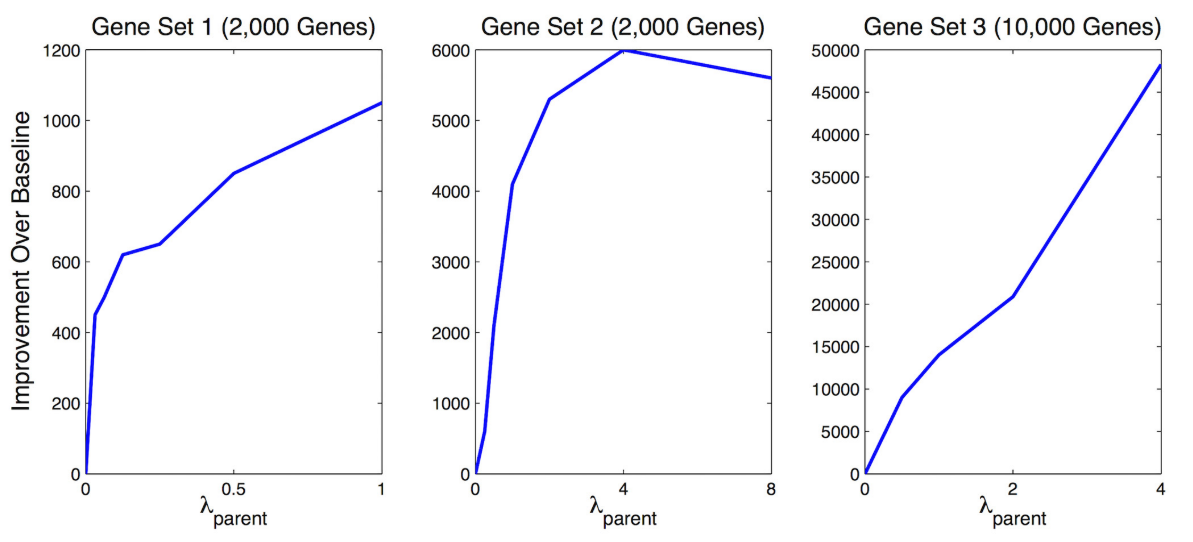
\includegraphics[width=0.85\linewidth]{slides/pierson_cv_likelihood.png}
  \caption{Improvement in cross-validated log likelihood over independent per-tissue graphical lasso ($\lambda_p=0$) as a function of the strength $\lambda_{\text{parent}}=\lambda_p$ of sharing along the tissue hierarchy, for three gene sets. Reproduced from \citet{pierson2015}.}
  \label{fig:pierson_cv}
\end{figure}

The tissue networks can then be compared, for example by finding clusters of genes that are densely connected in one tissue and not in others and testing each cluster for enrichment of gene sets with known function. \citet{pierson2015} report, for instance, a hippocampus-specific cluster enriched for synaptic vesicle genes. Such enrichments should be read with care. Enrichment tests need the right background set: genes expressed in brain are themselves enriched for synaptic functions, so a brain cluster tested against all genes will look enriched for synaptic terms whether or not the network is informative. More generally, validating an inferred network is hard because there is rarely a ground truth to compare against.

%======================================================================
\section{Network properties}
\label{sec:graph_properties}
%======================================================================

Once we have a network, whether measured or inferred, graph theory offers many summaries of its structure. Consider an undirected graph with $M$ nodes and adjacency matrix $\mA\in\{0,1\}^{M\times M}$, where $a_{ij}=a_{ji}=1$ if there is an edge between nodes $i$ and $j$ and $a_{ii}=0$. Let $|\mathcal{E}|=\sum_{i<j}a_{ij}$ be the number of edges. The \emph{degree} of node $i$ is the number of edges it has, $k_i=\sum_ja_{ij}$. Some properties describe the whole network and others describe individual nodes.

\begin{itemize}
  \item \emph{Density} (or sparsity). An undirected graph has $M(M-1)/2$ possible edges (a directed graph without self-loops has $M(M-1)$), and the density is $|\mathcal{E}|/\binom{M}{2}$. The number of possible edges grows as $O(M^2)$. A family of networks is called \emph{sparse} if the number of edges grows more slowly, for example as $O(M)$ or $O(M\log M)$, so that the mean degree $2|\mathcal{E}|/M$ stays small. Biological networks are sparse in this sense.
  \item \emph{Diameter}. The distance $d(a,b)$ between nodes $a$ and $b$ is the number of edges on a shortest path between them. The diameter is the largest distance between any two nodes, $\max_{a,b}d(a,b)$, computed within a connected component, since the distance between disconnected nodes is infinite. All distances from one node can be computed by breadth-first search in $O(M+|\mathcal{E}|)$ time, so the diameter takes $O(M(M+|\mathcal{E}|))$.
  \item \emph{Clustering coefficient}. For node $i$ with $k_i\ge2$ neighbours, the local clustering coefficient is the proportion of pairs of its neighbours that are themselves connected,
  \begin{equation}
    C_i = \frac{\sum_{j<l}a_{ij}a_{il}a_{jl}}{k_i(k_i-1)/2}.
  \end{equation}
  In social terms, it is the proportion of your friends who are friends with each other. The average of $C_i$ over nodes measures how clumped the network is.
  \item \emph{Betweenness centrality}. Let $\sigma_{st}$ be the number of shortest paths between nodes $s$ and $t$, and $\sigma_{st}(v)$ the number of those that pass through node $v$. The betweenness centrality of $v$ is
  \begin{equation}
    b(v) = \frac{1}{\binom{M-1}{2}}\sum_{s<t,\; s\neq v\neq t}\frac{\sigma_{st}(v)}{\sigma_{st}},
  \end{equation}
  the proportion of shortest paths through $v$, averaged over all pairs of other nodes. Nodes with high betweenness are bottlenecks or hubs of a transport network; in the British rail network, London would have very high betweenness, since many journeys pass through it. Brandes' algorithm computes $b(v)$ for all nodes in $O(M|\mathcal{E}|)$ time~\citep{brandes2001}.
  \item \emph{Degree distribution}. The histogram of degrees across nodes, $p(k)$, the fraction of nodes with degree $k$.
\end{itemize}

Figure~\ref{fig:betweenness} shows a random spatial network with $\btwNodes$ nodes and $\btwEdges$ edges, colored by betweenness. Its density is $\btwDensity$, its diameter $\btwDiameter$ and its average clustering coefficient $\btwClustering$; the clustering is high because nodes are connected when they are near each other, so neighbours of a node tend to be near each other too. The nodes with the highest betweenness, up to $\btwMaxBC$, are those that connect otherwise separate regions.

\begin{figure}[tbp]
  \centering
  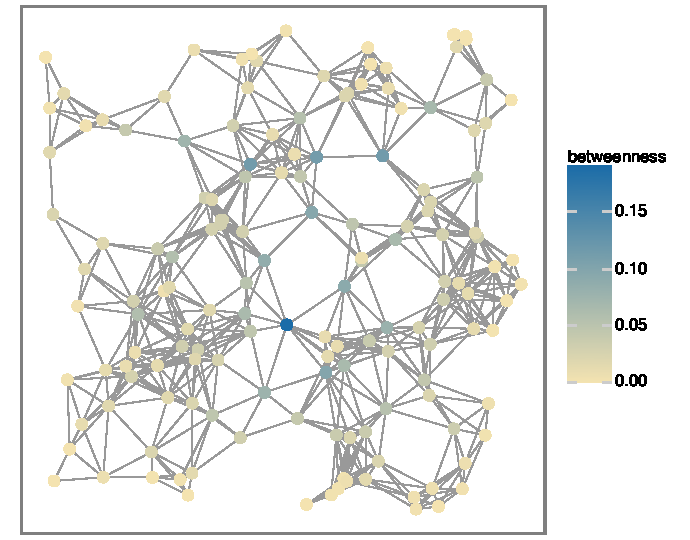
\includegraphics[width=0.6\linewidth]{betweenness.pdf}
  \caption{A random geometric graph (nodes placed uniformly in the unit square and connected if closer than 0.15; largest connected component shown), with nodes colored by betweenness centrality. Nodes that bridge different regions of the graph lie on many shortest paths.}
  \label{fig:betweenness}
\end{figure}

\subsection{Degree distributions and scale-free networks}

The simplest random graph model, the Erdős--Rényi model~\citep{erdos1959}, includes each of the $\binom M2$ possible edges independently with the same probability $p$. The degree of a node is then $\text{Binomial}(M-1,p)$, approximately Poisson with mean $(M-1)p$ for large $M$, and nodes with degree far above the mean are vanishingly rare. Many biological networks look different: most nodes have few edges, but a few hubs have very many. Such degree distributions are often described as \emph{scale-free}, following a power law
\begin{equation}
  p(k)\propto k^{-\gamma} \quad\Longleftrightarrow\quad \log p(k) = -\gamma\log k + \text{const},
\end{equation}
for some exponent $\gamma>0$, so that the distribution is a straight line on a log-log plot. \citet{reguly2006} found an approximately straight line for the degree distribution of literature-curated yeast genetic interactions, with the most connected genes having around 100 partners. A simple mechanism that produces power laws is \emph{preferential attachment}~\citep{barabasi1999}: the network grows one node at a time, and each new node connects to $m$ existing nodes chosen with probability proportional to their current degree, so that the rich get richer. Figure~\ref{fig:degree} compares the two models with the same number of nodes and the same mean degree. The largest degree is $\maxDegER$ under the Erdős--Rényi model and $\maxDegBA$ under preferential attachment.

\begin{figure}[tbp]
  \centering
  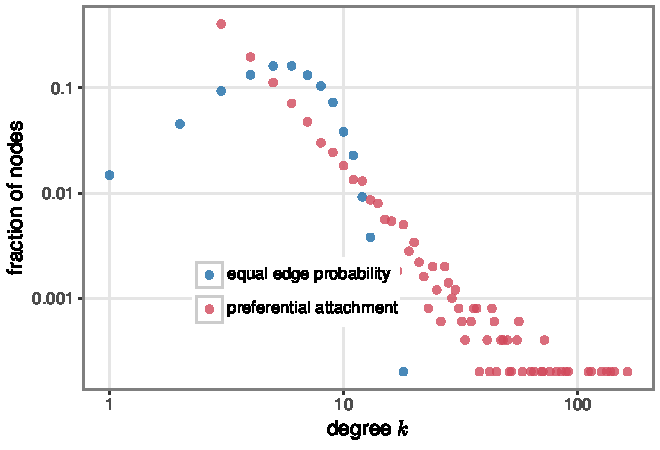
\includegraphics[width=0.6\linewidth]{degree_distribution.pdf}
  \caption{Degree distributions on log-log axes for two simulated networks with $M=5000$ nodes and mean degree 6: an Erdős--Rényi graph, in which every edge has equal probability (blue), and a preferential attachment graph (red, $m=3$). The Erdős--Rényi degree distribution is approximately Poisson and drops off quickly; preferential attachment gives an approximately straight line, a power law, with hubs of degree above 100.}
  \label{fig:degree}
\end{figure}

How widely biological networks are truly scale-free is debated. A systematic test of many networks found strong evidence for power laws in few of them~\citep{broido2019}, and degree distributions of measured networks are distorted by incomplete sampling: in PPI networks, well-studied proteins have more recorded interactions. It remains true that biological networks are much more heavy-tailed than the Erdős--Rényi model predicts.

%======================================================================
\section{Stochastic blockmodels}
\label{sec:sbm}
%======================================================================

The graphical lasso estimates a network from data. A different task is to model the structure of a given network, measured directly (like a PPI network) or estimated. A common structure is \emph{communities}: groups of nodes with many edges among themselves and fewer to the rest of the network. The \emph{stochastic blockmodel} (SBM)~\citep{holland1983,nowicki2001,abbe2018}, developed first for social networks, is a mixture model for this structure. It is to networks what a Gaussian mixture model, the probabilistic counterpart of $k$-means (Chapter 5), is to points.

\subsection{The generative model}

Let $K$ be the number of blocks (clusters, communities). The SBM generates an undirected network on $M$ nodes as follows.
\begin{enumerate}
  \item For each node $i=1,\dots,M$, draw a block assignment $c_i\sim\Cat(\vpi)$, where $\vpi\in\R^K$ is a probability vector; the simplest choice is $\vpi=[1/K,\dots,1/K]$, and $\vpi$ can instead be estimated or given a Dirichlet prior.
  \item For each pair of nodes $i<j$, draw the edge indicator
  \begin{equation}
    a_{ij}\mid c_i,c_j \sim \Bern\left(\eta_{c_ic_j}\right),
  \end{equation}
  and set $a_{ji}=a_{ij}$.
\end{enumerate}
Here $\veta\in[0,1]^{K\times K}$ is a symmetric matrix whose entry $\eta_{kl}$ is the probability of an edge between a node in block $k$ and a node in block $l$. A Bayesian version puts a prior $\eta_{kl}\sim\text{Beta}(a,b)$ on each entry. For example, with $K=3$,
\begin{equation}
  \veta = \begin{pmatrix} 0.5 & 0.01 & 0.01\\ 0.01 & 0.4 & 0.01\\ 0.01 & 0.01 & 0.6\end{pmatrix}
\end{equation}
describes three communities with dense connections within and sparse connections between them. A large diagonal is typical, an \emph{assortative} network, but nothing in the model requires it. A large off-diagonal entry describes two blocks that connect to each other more than to themselves, a \emph{disassortative} structure, as in a bipartite network between, say, enzymes and the metabolites they act on, or kinases and their substrates.

The joint probability of the assignments $\vc=(c_1,\dots,c_M)$ and the network is
\begin{equation}
  p(\mA,\vc\mid\vpi,\veta) = \prod_{i=1}^M\pi_{c_i}\prod_{i<j}\eta_{c_ic_j}^{a_{ij}}\left(1-\eta_{c_ic_j}\right)^{1-a_{ij}}.
  \label{eq:sbm_joint}
\end{equation}

\subsection{Inference}

As for a mixture model, the parameters can be fit by expectation maximization: an E step that infers the block assignments given $\veta$ and $\vpi$, and an M step that re-estimates $\veta$ and $\vpi$ given the assignments. There is one important difference from a Gaussian mixture. There, the posterior over assignments factorizes over data points. In the SBM each edge depends on the assignments of two nodes, so the posterior $p(\vc\mid\mA)$ couples all nodes and has $K^M$ configurations; the exact E step is intractable. The standard solution is \emph{variational EM}~\citep{daudin2008}: approximate the posterior by a factorized (mean-field) distribution $q(\vc)=\prod_iq_i(c_i)$, with $q_{ik}=q_i(c_i=k)$, and maximize the evidence lower bound
\begin{equation}
  \mathcal{L}(q,\vpi,\veta) = \E_q\left[\log p(\mA,\vc\mid\vpi,\veta)\right] - \E_q\left[\log q(\vc)\right].
\end{equation}
Taking the expectation of the log of~\eqref{eq:sbm_joint} under $q$,
\begin{equation}
  \E_q\left[\log p(\mA,\vc\mid\vpi,\veta)\right] = \sum_{i}\sum_kq_{ik}\log\pi_k + \sum_{i<j}\sum_{k,l}q_{ik}q_{jl}\left[a_{ij}\log\eta_{kl}+(1-a_{ij})\log(1-\eta_{kl})\right].
\end{equation}
\emph{M step.} Setting the derivative with respect to $\eta_{kl}$ to zero, and writing the sum over pairs as half a sum over ordered pairs $i\neq j$ to handle the symmetry of $\veta$,
\begin{equation}
  \hat\eta_{kl} = \frac{\sum_{i\neq j}q_{ik}q_{jl}a_{ij}}{\sum_{i\neq j}q_{ik}q_{jl}},
  \qquad \hat\pi_k = \frac1M\sum_iq_{ik},
\end{equation}
the expected number of edges between blocks $k$ and $l$ divided by the expected number of pairs. (The update for $\vpi$ uses a Lagrange multiplier for $\sum_k\pi_k=1$, as in Chapter 5.)

\emph{E step.} Holding all other factors fixed, the optimal $q_i$ is proportional to the exponentiated expected log joint, with the expectation taken over all other nodes,
\begin{equation}
  \log q_{ik} = \log\pi_k + \sum_{j\neq i}\sum_lq_{jl}\left[a_{ij}\log\eta_{kl}+(1-a_{ij})\log(1-\eta_{kl})\right] + \text{const},
\end{equation}
normalized so that $\sum_kq_{ik}=1$. Node $i$ is assigned to blocks whose connection pattern, given the soft assignments of all other nodes, best explains its row of $\mA$. These updates are iterated to convergence. Since $\mathcal{L}$ is not concave, several initializations, for example from spectral clustering (k-means on the leading eigenvectors of $\mA$), are used and the solution with the highest bound kept.

Figure~\ref{fig:sbm} applies this algorithm to a network of $M=120$ nodes simulated from an SBM with $K=4$ blocks: two assortative communities and a disassortative pair of blocks that connect mostly to each other. In the original node order, panel (a), no structure is visible. Ordering the nodes by their inferred block reveals it. The inferred blocks match the true ones exactly (adjusted Rand index $\sbmARI$), and, with blocks in the order shown in panel (b), the estimated edge probabilities are
\begin{equation}
  \hat\veta = \begin{pmatrix} \sbmEtaHat \end{pmatrix},
\end{equation}
close to the simulated values of 0.40 and 0.35 within the assortative blocks, 0.30 between the disassortative pair, and 0.03 to 0.04 elsewhere.

\begin{figure}[tbp]
  \centering
  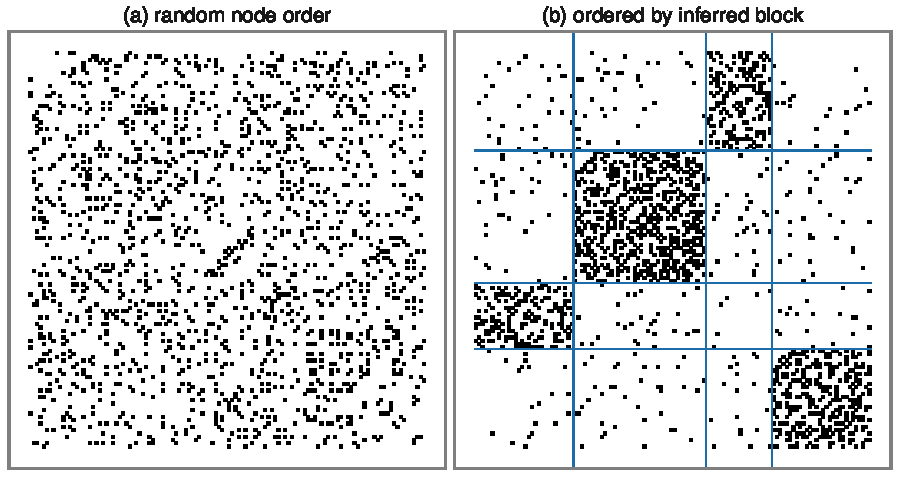
\includegraphics[width=0.85\linewidth]{sbm_adjacency.pdf}
  \caption{A stochastic blockmodel fit to a simulated network ($M=120$ nodes, $K=4$ blocks). Black entries of the adjacency matrix are edges. (a) Nodes in random order. (b) Nodes ordered by the blocks inferred by variational EM, with block boundaries in blue. Two blocks are assortative (dense diagonal blocks); the other two connect mainly to each other (dense off-diagonal blocks).}
  \label{fig:sbm}
\end{figure}

\subsection{Choosing the number of blocks}

The \emph{infinite relational model}~\citep{kemp2006} is a Bayesian nonparametric SBM. It places a Chinese restaurant process prior on the partition of nodes into blocks, which allows an unbounded number of blocks, and infers the number of blocks used by the data along with the assignments, typically by Markov chain Monte Carlo. It also handles several relations and directed relations at once. Bayesian nonparametric models of this kind have elegant mathematics but can be awkward in practice; a common alternative is to fit a model with generous $K$ and prune blocks that receive few nodes, or to compare values of $K$ by held-out likelihood or an information criterion.

\subsection{Predicting missing edges}

Because PPI networks have many false negatives, a natural use of a network model is \emph{link prediction}: scoring pairs of proteins with no recorded interaction by how likely an interaction is. Under a fitted SBM, the predicted probability of an edge between $i$ and $j$ is
\begin{equation}
  p(a_{ij}=1\mid\mA_{\text{obs}}) \approx \sum_{k,l}q_{ik}q_{jl}\hat\eta_{kl}.
\end{equation}
Blockmodels predict missing PPIs better than random guessing, though methods that use additional information, such as protein sequence, structure and co-expression, usually do better.

%======================================================================
\section{Mixed membership stochastic blockmodels}
\label{sec:mmsb}
%======================================================================

In the SBM, as in $k$-means, each node belongs to exactly one block. This is restrictive. In a social network you may have many friends at your university, but also friends from a sport you play and from a school you went to; no single community describes you. Many proteins likewise take part in several complexes or processes. Matrix factorization (Chapter 8) handles this by representing each object with several factors. \emph{Mixed membership} models instead represent each object by a probability distribution over clusters.

The mixed membership stochastic blockmodel (MMSB)~\citep{airoldi2008} replaces the block assignment $c_i$ of node $i$ with a membership vector $\vc_i\in\R^K$, with $c_{ik}\ge0$ and $\sum_kc_{ik}=1$. The generative model is as follows.
\begin{enumerate}
  \item For each node $i$, draw $\vc_i\sim\Dir([1,\dots,1])$. The Dirichlet distribution (Chapter 10) is the standard distribution on probability vectors; with all parameters equal to one it is uniform over the probability simplex.
  \item For each ordered pair of nodes $(i,j)$:
  \begin{enumerate}
    \item draw the block node $i$ acts in for this interaction, $z_{i\to j}\sim\Cat(\vc_i)$;
    \item draw the block node $j$ acts in, $z_{i\leftarrow j}\sim\Cat(\vc_j)$;
    \item draw the edge $a_{ij}\sim\Bern\big(\eta_{z_{i\to j},\,z_{i\leftarrow j}}\big)$.
  \end{enumerate}
\end{enumerate}
In the social example, my membership vector puts weight on ``Columbia faculty'' and on ``climbing''. For a particular person $j$, I draw one of my communities, say Columbia faculty; $j$, whose memberships are, say, Columbia faculty and cycling, draws one of theirs. The chance of a friendship is the entry of $\veta$ for that pair of communities, high if both drew the same community. Each pair gets its own draws, so different edges of a node can be explained by different communities.

Summing over the two indicators gives the probability of an edge given the memberships,
\begin{equation}
  p(a_{ij}=1\mid\vc_i,\vc_j,\veta) = \sum_{k=1}^K\sum_{l=1}^Kp(z_{i\to j}=k)\,p(z_{i\leftarrow j}=l)\,\eta_{kl} = \sum_{k,l}c_{ik}\eta_{kl}c_{jl} = \vc_i^\top\veta\,\vc_j .
\end{equation}
Collecting the memberships as rows of a matrix $\mathbf{C}\in\R^{M\times K}$, the matrix of edge probabilities is $\mathbf{C}\veta\mathbf{C}^\top$, a low-rank, non-negative factorization of the kind seen in Chapter 8. If every $\vc_i$ is a one-hot vector the MMSB reduces to the SBM.

Inference is again by variational EM, with an E step for the indicators $z$ (and the posterior over the memberships $\vc_i$) and an M step for $\veta$. \citet{airoldi2008} applied the MMSB to a yeast PPI network and used the inferred memberships to predict proteins' functional annotations, more accurately than random annotation baselines. The MMSB has the same structure as latent Dirichlet allocation (LDA)~\citep{blei2003}, the standard topic model for text before large language models: a document has a distribution over topics and each word is generated from one topic drawn from it, as a node has a distribution over communities and each interaction uses one community drawn from it. Figure~\ref{fig:sbm_gm} compares the SBM and MMSB as graphical models.

\begin{figure}[tbp]
  \centering
  \begin{tikzpicture}[>=Stealth, every node/.style={font=\small},
      lat/.style={draw, circle, minimum size=0.85cm, inner sep=1pt},
      obs/.style={draw, circle, fill=gray!25, minimum size=0.85cm, inner sep=1pt},
      par/.style={draw, rectangle, minimum size=0.6cm, inner sep=2pt}]
    \node at (-0.5,3.0) {(a) SBM};
    \node[par] (pi) at (1.5,2.3) {$\vpi$};
    \node[lat] (ci) at (0.5,1.0) {$c_i$};
    \node[lat] (cj) at (2.5,1.0) {$c_j$};
    \node[obs] (a) at (1.5,-0.4) {$a_{ij}$};
    \node[par] (eta) at (3.4,-0.4) {$\veta$};
    \draw[->] (pi) -- (ci); \draw[->] (pi) -- (cj);
    \draw[->] (ci) -- (a); \draw[->] (cj) -- (a); \draw[->] (eta) -- (a);
    \begin{scope}[xshift=6.3cm]
      \node at (-1.1,3.0) {(b) MMSB};
      \node[lat] (ci) at (0.3,2.3) {$\vc_i$};
      \node[lat] (cj) at (2.9,2.3) {$\vc_j$};
      \node[lat] (zi) at (0.3,0.95) {$z_{i\to j}$};
      \node[lat] (zj) at (2.9,0.95) {$z_{i\leftarrow j}$};
      \node[obs] (a) at (1.6,-0.4) {$a_{ij}$};
      \node[par] (eta) at (3.6,-0.4) {$\veta$};
      \draw[->] (ci) -- (zi); \draw[->] (cj) -- (zj);
      \draw[->] (zi) -- (a); \draw[->] (zj) -- (a); \draw[->] (eta) -- (a);
    \end{scope}
  \end{tikzpicture}
  \caption{Graphical models for one pair of nodes $(i,j)$. Shaded circles are observed, open circles latent, squares parameters. (a) In the stochastic blockmodel each node has a single block $c_i$, shared by all its edges. (b) In the mixed membership SBM each node has a membership vector $\vc_i$, and each interaction draws its own blocks $z_{i\to j}$ and $z_{i\leftarrow j}$ from the two nodes' memberships.}
  \label{fig:sbm_gm}
\end{figure}

%======================================================================
\section{Summary}
%======================================================================

\begin{itemize}
  \item ``Network'' means different things in biology; always ask what the nodes and edges are. Gene regulatory networks link transcription factors to their target genes (directed, signed); co-expression networks link co-regulated genes (undirected, inferred); protein-protein interaction networks link physically binding proteins; genetic interaction networks link genes whose double mutants deviate from the multiplicative expectation $f_if_j$; metabolic networks link metabolites through enzymatic reactions; signaling networks link kinases and other signaling molecules.
  \item Correlation mixes direct and indirect association. The partial correlation of two variables given all others is $-\theta_{ij}/\sqrt{\theta_{ii}\theta_{jj}}$, where $\mTheta$ is the precision matrix; for Gaussian data a zero entry means conditional independence.
  \item The graphical lasso estimates a sparse precision matrix by minimizing $-\log|\mTheta|+\tr(\mTheta\hSigma)+\lambda\|\mTheta\|_1$. It is convex, works when $N<P$, is fit by block coordinate descent over lasso subproblems, and $\lambda$ can be chosen by cross-validated likelihood.
  \item Networks for related tissues can be estimated jointly by penalizing differences between precision matrices along a tissue hierarchy, which improves held-out likelihood in GTEx.
  \item Network properties from graph theory include density, diameter, clustering coefficient, betweenness centrality and the degree distribution, which in biological networks is heavy-tailed.
  \item Stochastic blockmodels are mixture models for networks, fit by variational EM, and can predict missing edges. Mixed membership SBMs let each node belong to several communities, with edge probability $\vc_i^\top\veta\vc_j$.
\end{itemize}

%======================================================================
\section*{Exercises}
%======================================================================

\begin{enumerate}
  \item Let $x_1\sim\Normal(0,1)$, $x_2=ux_1+\epsilon_2$ and $x_3=vx_2+\epsilon_3$ for scalars $u,v\neq0$, with independent $\epsilon_2,\epsilon_3\sim\Normal(0,1)$. Compute the covariance matrix $\mSigma$ and the precision matrix $\mTheta$ of $(x_1,x_2,x_3)$. Show that $\Sigma_{13}\neq0$ but $\theta_{13}=0$, and interpret.
  \item Using the block matrix inversion formula, show that the coefficients of the population regression of $x_A$ on all other variables are $\beta_{Aj}=-\theta_{Aj}/\theta_{AA}$ and that the residual variance is $1/\theta_{AA}$.
  \item Show that $-\log|\mTheta|$ is convex on the set of positive definite matrices. (Hint: restrict to a line $\mTheta+t\mathbf{V}$ and write the function in terms of the eigenvalues of $\mTheta^{-1/2}\mathbf{V}\mTheta^{-1/2}$.)
  \item For the tissue hierarchy objective~\eqref{eq:gtex_objective} with $K=2$ tissues joined at a root, show that for fixed leaves the optimal root matrix is $\frac12(\mTheta^{(1)}+\mTheta^{(2)})$, and that the penalty then equals $\frac{\lambda_p}{2}\|\mTheta^{(1)}-\mTheta^{(2)}\|_2^2$.
  \item Compute the degree, clustering coefficient and betweenness centrality of every node in a star graph (one centre connected to $M-1$ leaves) and in a cycle of $M$ nodes. What are the diameters?
  \item Derive the M-step update for $\eta_{kl}$ in the SBM and show that when the $q_{ik}$ are one-hot it is the number of edges between blocks $k$ and $l$ divided by the number of node pairs between them.
  \item Implement the graphical lasso with cross-validation on the expression of a few hundred genes from one GTEx tissue. How does the number of edges at the cross-validated $\lambda$ change if you first regress out the top five principal components?
\end{enumerate}

\bibliographystyle{abbrvnat}
\bibliography{../chapter09/chapter09}
\endgroup

% Generated wrapper: chapter 10 with its own figure path, macros and bibliography.
\graphicspath{{../chapter10/figures/}}
\makeatletter\def\input@path{{../chapter10/}}\makeatother
\begingroup
% Chapter 10: RNA splicing, isoform quantification and sequence models of splicing.
% Requires: amsmath, amssymb, bm, graphicx, booktabs, subcaption, algorithm, algpseudocode,
% tikz (arrows.meta, positioning, calc, decorations.pathreplacing, fit), natbib.
% Computed figures are produced by scripts/make_figures.py;
% figures/slides/ holds figures taken from the lecture slides.

\providecommand{\R}{\mathbb{R}}
\providecommand{\E}{\mathbb{E}}
\providecommand{\Normal}{\mathcal{N}}
\providecommand{\argmax}{\operatorname*{arg\,max}}
\providecommand{\argmin}{\operatorname*{arg\,min}}
\providecommand{\vy}{\mathbf{y}}
\providecommand{\vx}{\mathbf{x}}
\providecommand{\mX}{\mathbf{X}}
\providecommand{\mI}{\mathbf{I}}
\providecommand{\vb}{\boldsymbol{\beta}}
\providecommand{\veps}{\boldsymbol{\epsilon}}
\providecommand{\vp}{\mathbf{p}}
\providecommand{\vg}{\mathbf{g}}
\providecommand{\ind}{\mathbf{1}}
\providecommand{\vpi}{\boldsymbol{\pi}}
\providecommand{\vu}{\mathbf{u}}
\providecommand{\mSigma}{\boldsymbol{\Sigma}}
\providecommand{\mLambda}{\boldsymbol{\Lambda}}
\providecommand{\KL}{\operatorname{KL}}
\providecommand{\vtheta}{\boldsymbol{\theta}}
\providecommand{\valpha}{\boldsymbol{\alpha}}
\providecommand{\vphi}{\boldsymbol{\phi}}
\providecommand{\veta}{\boldsymbol{\eta}}
\providecommand{\vz}{\mathbf{z}}
\providecommand{\mZ}{\mathbf{Z}}
\providecommand{\vr}{\mathbf{r}}
\providecommand{\va}{\mathbf{a}}
\providecommand{\vmu}{\boldsymbol{\mu}}
\providecommand{\Dir}{\operatorname{Dir}}
\providecommand{\Disc}{\operatorname{Discrete}}
\providecommand{\Bin}{\operatorname{Binomial}}
\providecommand{\BetaD}{\operatorname{Beta}}
\providecommand{\simplex}{\Delta}

\providecommand{\chaptertoc}{}
\chapter{RNA splicing}
\label{ch:splicing}
\chaptertoc

The central dogma of Chapter 1 says that DNA is transcribed into RNA and RNA is translated into protein. In humans and other eukaryotes there is a step in between. The RNA that RNA polymerase II produces is a \emph{precursor}: before it leaves the nucleus it is capped, cut and polyadenylated, and most of its length, the \emph{introns}, is removed by \emph{splicing}. Which segments are removed can vary between cell types and conditions, so one gene can produce several distinct RNA molecules, its \emph{isoforms}, which may encode different proteins.

This chapter covers three things. The first is the biology: what a gene looks like, how RNA is processed, and how alternative splicing generates isoforms that matter in health and disease. The second is a statistical problem. Short-read RNA-seq breaks RNA into fragments that are much shorter than isoforms, so the abundance of each isoform has to be inferred. We set up a generative model of reads, fit it by expectation maximization (EM), and then use the same model to introduce variational Bayesian inference: coordinate ascent variational inference (CAVI) and its stochastic extensions, which underlie variational autoencoders. The third is prediction of splicing from DNA sequence, from feature-based models of exon inclusion to SpliceAI, a deep residual network of dilated convolutions, and models trained on millions of synthetic sequences. We end with long-read sequencing, which reads whole isoforms directly.

%======================================================================
\section{Gene structure and RNA processing}
\label{sec:gene_structure}
%======================================================================

\subsection{Anatomy of a gene}

Figure~\ref{fig:gene_anatomy} shows the parts of a typical human protein-coding gene. The description is specific to vertebrates; genes in bacteria, and to a lesser extent in yeast, are organized differently. Transcription starts at the \emph{transcription start site} (TSS), just downstream of the promoter that we met in earlier chapters, and ends near the \emph{transcription end site} (TES). The transcribed region is divided into \emph{exons}, the segments that remain in the mature RNA, and \emph{introns}, the segments between them, which are removed by splicing. Walter Gilbert, who coined the terms, derived them from \emph{ex}pressed regions and \emph{in}tragenic regions~\citep{gilbert1978}.

Not every exonic nucleotide codes for protein. Translation starts at a start codon (AUG) some way into the first exon(s) and ends at a stop codon in the last exon. The exonic sequence before the start codon is the $5'$ \emph{untranslated region} (UTR) and the sequence after the stop codon is the $3'$ UTR. UTRs have regulatory roles. The $5'$ UTR affects how efficiently the RNA is translated, which is why therapeutic RNA design often optimizes it. The $3'$ UTR contains binding sites for RNA-binding proteins and microRNAs that control the stability and localization of the RNA.

\begin{figure}[!htbp]
  \centering
  \begin{tikzpicture}[>=Stealth, every node/.style={font=\small}, x=0.95cm, y=1cm]
    % gene line
    \draw[thick] (-0.6,0) -- (13.2,0);
    \node[left] at (-0.6,0) {$5'$};
    \node[right] at (13.2,0) {$3'$};
    % promoter
    \draw[fill=orange!40] (0.0,-0.12) rectangle (0.8,0.12);
    \node[below=4pt, font=\footnotesize] at (0.4,-0.1) {promoter};
    % TSS
    \draw[->, thick, green!50!black] (1.2,0.15) -- (1.2,0.55) -- (1.7,0.55);
    \node[above] at (1.2,0.55) {TSS};
    % exon 1: UTR + CDS
    \draw[fill=blue!12] (1.2,-0.22) rectangle (1.9,0.22);
    \draw[fill=blue!45] (1.9,-0.22) rectangle (2.6,0.22);
    % intron 1
    \draw[decorate, decoration={brace, amplitude=4pt}] (2.65,0.35) -- (6.95,0.35) node[midway, above=4pt] {intron, $\sim$3.5\,kb};
    % exon 2
    \draw[fill=blue!45] (7.0,-0.22) rectangle (7.6,0.22);
    \node[above=3pt, font=\footnotesize, align=center] at (7.3,0.25) {exon\\$\sim$150\,nt};
    % intron 2
    \node[above, font=\footnotesize] at (9.0,0.05) {intron};
    % exon 3: CDS + UTR
    \draw[fill=blue!45] (10.4,-0.22) rectangle (10.9,0.22);
    \draw[fill=blue!12] (10.9,-0.22) rectangle (12.6,0.22);
    \draw[->, thick, red!70!black] (12.6,0.15) -- (12.6,0.55);
    \node[above] at (12.6,0.55) {TES};
    % braces below
    \draw[decorate, decoration={brace, mirror, amplitude=4pt}] (1.2,-0.32) -- (1.9,-0.32) node[midway, below=5pt, font=\footnotesize, align=center] {$5'$ UTR\\$\sim$200\,nt};
    \draw[decorate, decoration={brace, mirror, amplitude=4pt}] (10.9,-0.32) -- (12.6,-0.32) node[midway, below=5pt, font=\footnotesize, align=center] {$3'$ UTR\\$\sim$800\,nt};
    \draw[->] (2.3,1.0) node[above, font=\footnotesize] {start codon} -- (1.92,0.27);
    \draw[->] (10.3,1.0) node[above, font=\footnotesize] {stop codon} -- (10.88,0.27);
    \draw[->] (13.9,-1.2) node[below, font=\footnotesize] {poly(A) signal} -- (12.3,-0.25);
    % zoom on intron 1
    \draw[dashed, gray] (2.6,-0.25) -- (0.6,-2.2);
    \draw[dashed, gray] (7.0,-0.25) -- (12.6,-2.2);
    \begin{scope}[yshift=-2.8cm]
      \draw[fill=blue!45] (0.0,-0.22) rectangle (1.6,0.22);
      \draw[fill=blue!45] (11.4,-0.22) rectangle (13.0,0.22);
      \draw[thick] (1.6,0) -- (11.4,0);
      \node[above=2pt, font=\footnotesize] at (0.8,0.22) {exon};
      \node[above=2pt, font=\footnotesize] at (12.2,0.22) {exon};
      \node[above=2pt, font=\footnotesize] at (6.5,0.0) {intron};
      % donor
      \node[below=3pt, font=\ttfamily\footnotesize] (don) at (1.6,-0.25) {CAG|GUAAGU};
      \node[below=0pt, font=\footnotesize, align=center] at (don.south) {$5'$ splice site\\(donor)};
      % branch point
      \node[below=3pt, font=\ttfamily\footnotesize] (bp) at (8.0,-0.25) {YNYURAY};
      \node[below=0pt, font=\footnotesize, align=center] at (bp.south) {branch point\\18--40\,nt upstream};
      \draw[fill=black] (8.0,0) circle (0.06);
      % polypyrimidine tract
      \draw[line width=2.5pt, orange!70] (9.2,0) -- (10.7,0);
      \node[above=2pt, font=\footnotesize] at (9.95,0.0) {poly-Y tract};
      % acceptor
      \node[below=3pt, font=\ttfamily\footnotesize] (acc) at (11.4,-0.25) {NCAG|G};
      \node[below=0pt, font=\footnotesize, align=center] at (acc.south) {$3'$ splice site\\(acceptor)};
    \end{scope}
  \end{tikzpicture}
  \caption{Anatomy of a human protein-coding gene (not to scale). Top: transcription runs from the TSS to the TES. Exons (boxes) contain the coding sequence (dark) and the $5'$ and $3'$ UTRs (light); introns (lines) are removed by splicing. Typical lengths are indicated; they vary by orders of magnitude between genes~\citep{piovesan2016}. Bottom: consensus sequences at an intron, written in RNA, with $|$ marking the exon-intron boundary. The intron almost always begins with GU and ends with AG. Y is a pyrimidine (C or U), R a purine (A or G), N any nucleotide; the A after R in the branch point consensus is the branch point adenosine.}
  \label{fig:gene_anatomy}
\end{figure}

Some scales are worth keeping in mind~\citep{piovesan2016}. A typical human gene has around ten exons. A few have more than a hundred, and a small fraction have a single exon and no introns. A typical internal exon is about 150 nucleotides (nt) long. The genetic code reads three nucleotides (a codon) per amino acid, so an average exon encodes about 50 amino acids. Introns are much longer: a typical intron is several kilobases (kb), of the order of 3.5\,kb, and some are hundreds of kilobases. The cell therefore transcribes long precursor RNAs and discards most of each one. Why splicing evolved in this form is not settled, but introns are not simply waste: much of the sequence that regulates splicing lies in them.

\subsection{RNA processing}

Three processing steps convert the nascent transcript into a mature messenger RNA (mRNA)~\citep{desterro2020}, and they mostly happen \emph{co-transcriptionally}, while RNA polymerase II (Pol II) is still transcribing the gene (Figure~\ref{fig:mrna_processing}).
\begin{enumerate}
  \item \emph{$5'$ capping.} Shortly after transcription starts, the $5'$ end of the RNA emerges from Pol II and a capping complex adds a modified guanosine, 7-methylguanosine (m$^7$G). The cap is bound by the cap-binding complex, which protects the RNA from degradation and later helps recruit the ribosome.
  \item \emph{Splicing.} As Pol II moves through the gene, the \emph{spliceosome}, a large complex of RNAs and proteins, excises the introns and joins the exons.
  \item \emph{$3'$ end formation.} Near the end of the gene, the cleavage and polyadenylation complex recognizes the polyadenylation signal (consensus AAUAAA) in the $3'$ UTR, cleaves the RNA and adds a tail of adenosines, the poly(A) tail, which also stabilizes the RNA.
\end{enumerate}
The mature mRNA is then exported from the nucleus, translated in the cytoplasm, and eventually degraded at a rate that differs between RNAs. Each of these steps is a point of regulation that the simple central dogma leaves out. The long C-terminal domain (CTD) of Pol II, drawn in green in Figure~\ref{fig:mrna_processing}, is a flexible tail that recruits capping, splicing and polyadenylation factors, which is one way the steps are coupled to transcription.

\begin{figure}[!htbp]
  \centering
  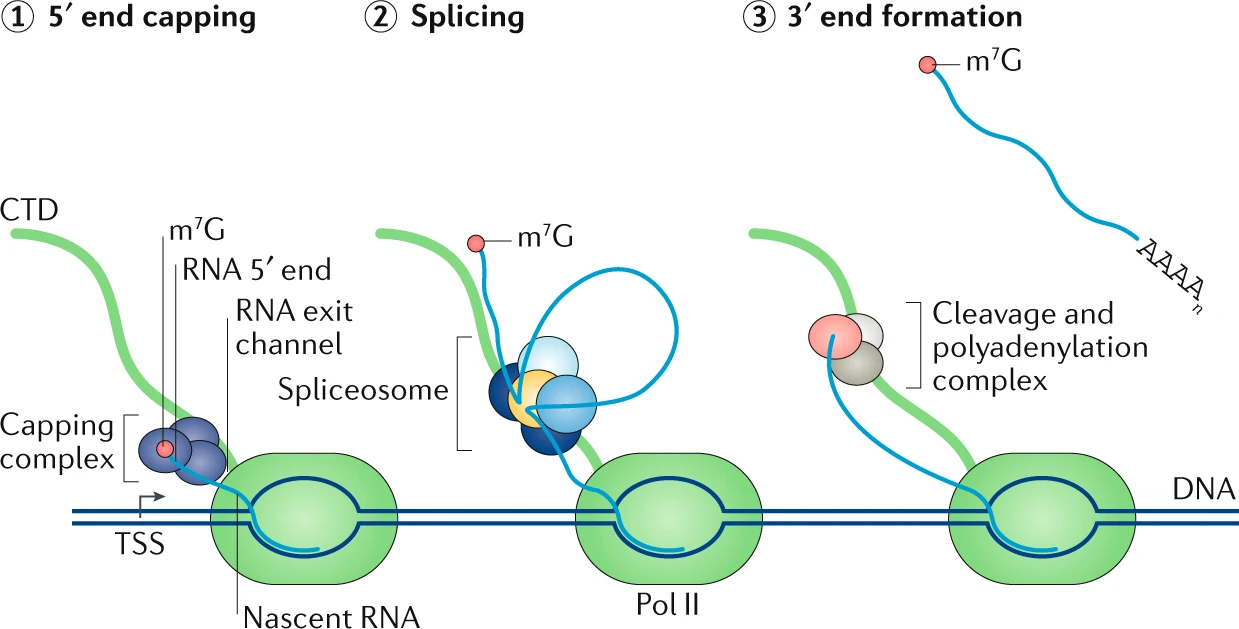
\includegraphics[width=0.85\linewidth]{slides/mrna_processing.png}
  \caption{Co-transcriptional mRNA processing by RNA polymerase II (Pol II): (1) $5'$ capping with 7-methylguanosine (m$^7$G), (2) splicing by the spliceosome, and (3) cleavage and polyadenylation. CTD, C-terminal domain of Pol II; TSS, transcription start site. Reproduced from \citet{desterro2020}.}
  \label{fig:mrna_processing}
\end{figure}

\subsection{The splicing reaction}

Splicing removes an intron in two chemical steps (Figure~\ref{fig:splicing_reaction}). Three sequence features of the intron are essential: the GU dinucleotide at its $5'$ end (the \emph{splice donor}), the AG dinucleotide at its $3'$ end (the \emph{splice acceptor}), and an adenosine at the \emph{branch point}, typically 18--40\,nt upstream of the acceptor. In the first step, the branch point A attacks the G at the start of the intron. This cuts the RNA at the donor and joins the start of the intron to the branch point, making a looped structure called a \emph{lariat}. In the second step, the free end of the upstream exon attacks the acceptor, which joins the two exons and releases the intron as a lariat, which is then degraded. Mutations of the GU, the AG or the branch point usually disrupt splicing of the intron, often with severe consequences for the protein.

\begin{figure}[!htbp]
  \centering
  \begin{tikzpicture}[>=Stealth, every node/.style={font=\small}]
    \tikzset{exon/.style={fill=red!60!black, draw=none}}
    % pre-mRNA
    \node[left] at (-0.2,0) {pre-mRNA};
    \draw (-0.2,0) -- (0,0);
    \fill[exon] (0,-0.15) rectangle (2.4,0.15);
    \draw (2.4,0) -- (7.2,0);
    \fill[exon] (7.2,-0.15) rectangle (9.6,0.15);
    \draw (9.6,0) -- (9.8,0);
    \node[fill=white, inner sep=1pt] (gu) at (2.75,0) {GU};
    \node[fill=white, inner sep=1pt] (a1) at (5.6,0) {A};
    \node[fill=white, inner sep=1pt] at (6.85,0) {AG};
    \node[above] at (1.2,0.15) {exon 1};
    \node[above] at (4.8,0.1) {intron};
    \node[above] at (8.4,0.15) {exon 2};
    \node[below=6pt] at (5.6,-0.1) {branch point};
    \draw[->, red!70!black, thick] (a1.south west) to[out=-150, in=-30] node[below, pos=0.6] {(1)} (gu.south);
    \draw[->, very thick] (4.8,-1.0) -- (4.8,-1.6);
    % intermediate
    \begin{scope}[yshift=-2.6cm]
      \fill[exon] (0,-0.15) rectangle (2.4,0.15);
      \draw (2.4,0) -- (2.6,0);
      \draw (5.6,0) circle (0.0);
      \draw[thick] (5.45,0.0) arc[start angle=0, end angle=330, radius=0.55];
      \node[fill=white, inner sep=1pt] (a2) at (5.6,0) {A};
      \draw (5.8,0) -- (6.6,0);
      \node[fill=white, inner sep=1pt] at (6.85,0) {AG};
      \draw (7.05,0) -- (7.2,0);
      \fill[exon] (7.2,-0.15) rectangle (9.6,0.15);
      \node[font=\footnotesize] at (4.45,-0.85) {lariat};
      \draw[->, red!70!black, thick] (2.4,0.25) to[out=40, in=140] node[above] {(2)} (7.15,0.25);
    \end{scope}
    \draw[->, very thick] (4.8,-3.7) -- (4.8,-4.3);
    % products
    \begin{scope}[yshift=-5.0cm]
      \node[left] at (1.0,0) {spliced mRNA};
      \fill[exon] (1.0,-0.15) rectangle (3.4,0.15);
      \fill[exon] (3.42,-0.15) rectangle (5.8,0.15);
      \node at (6.6,0) {$+$};
      \draw[thick] (8.15,0.0) arc[start angle=0, end angle=330, radius=0.5];
      \node[fill=white, inner sep=1pt] at (8.3,0) {A};
      \draw (8.5,0) -- (9.0,0) node[right] {AG};
      \node[font=\footnotesize] at (7.7,-0.75) {excised lariat};
    \end{scope}
  \end{tikzpicture}
  \caption{The two steps of splicing. (1) The branch point adenosine attacks the G of the GU at the $5'$ end of the intron, cutting at the donor and forming a lariat. (2) The free end of exon 1 attacks the acceptor AG, joining the exons and releasing the intron lariat.}
  \label{fig:splicing_reaction}
\end{figure}

The consensus sequences around the splice sites extend beyond the GU and AG (Figure~\ref{fig:gene_anatomy}, bottom). Around the donor the consensus is CAG$|$GUAAGU, where $|$ is the exon-intron boundary; the GU is almost invariant, while the other positions are only preferred. Upstream of the acceptor lies a \emph{polypyrimidine tract}, a run of C and U, and the acceptor itself has the consensus NCAG$|$G. These letters use the IUPAC code for degenerate nucleotides, in which Y stands for a pyrimidine (C or U, T in DNA), R for a purine (A or G) and N for any nucleotide. The consensus alone does not specify the splice sites: sequences resembling splice sites are common in introns, and most are not used. How the spliceosome picks the right ones is the subject of Section~\ref{sec:seq_models}.

\subsection{Alternative splicing}

When the choice of which segments to remove as introns varies, a gene produces more than one isoform. This is \emph{alternative splicing}. It affects most human multi-exon genes, it can differ between tissues, cell types and conditions, and it increases the number of distinct proteins that a genome can encode.

\paragraph{An example: tau.} The protein tau binds and stabilizes \emph{microtubules}, the polymers that form the cell's internal transport network. They matter most in neurons (Figure~\ref{fig:tau}a). A neuron's cell body is of the order of 50\,$\mu$m across, but its axon, the projection that carries its output signal to synapses, can be up to a metre long. Most RNA and protein is made in or near the cell body, so cargo, including RNA, has to be carried along the axon. Motor proteins called kinesins walk along microtubules carrying this cargo, and tau keeps the tracks intact.

Tau is encoded by the gene \textit{MAPT} (microtubule-associated protein tau); gene and protein names often differ in this way. The best-studied alternative splicing event in \textit{MAPT} is the inclusion or skipping of exon 10, which encodes one of the protein's microtubule-binding repeats (Figure~\ref{fig:tau}b). Skipping exon 10 gives isoforms with three repeats (3R tau), and including it gives isoforms with four repeats (4R tau), which bind microtubules more strongly~\citep{goedert1989}. The balance between 3R and 4R is regulated during development: fetal brain expresses mostly 3R tau, and adult brain expresses 3R and 4R in roughly equal amounts. Mutations that disturb this balance cause disease. Frontotemporal dementia with parkinsonism linked to chromosome 17 (FTDP-17), for example, can be caused by mutations in \textit{MAPT}, some of them near the $5'$ splice site of exon 10, which increase its inclusion and so the proportion of 4R tau~\citep{hutton1998}. Tau is involved in a family of neurodegenerative diseases called tauopathies, and aggregates of tau are a hallmark of Alzheimer's disease.

\begin{figure}[!htbp]
  \centering
  \begin{tikzpicture}[>=Stealth, every node/.style={font=\small}]
    \node at (-1.9,2.3) {(a)};
    % neuron schematic
    \draw[fill=orange!25, draw=orange!60!black] (0.8,1.2) circle (0.55);
    \draw[fill=orange!60, draw=none] (0.85,1.25) circle (0.18);
    \foreach \a in {100,150,200,250} \draw[orange!60!black, thick] ({0.8+0.55*cos(\a)},{1.2+0.55*sin(\a)}) -- ({0.8+1.0*cos(\a)},{1.2+1.0*sin(\a)});
    \draw[orange!60!black, line width=3pt] (1.35,1.2) -- (5.6,1.2);
    \foreach \a in {-40,-15,15,40} \draw[orange!60!black, thick] (5.6,1.2) -- ++(\a:0.6);
    \node[left] at (-0.25,1.2) {cell body};
    \node[above] at (3.5,1.3) {axon};
    \draw[decorate, decoration={brace, mirror, amplitude=3pt}] (0.25,0.35) -- (1.35,0.35) node[midway, below=3pt, font=\footnotesize] {$\sim$50\,$\mu$m};
    \node[right, font=\footnotesize] at (6.2,1.2) {synapses};
    % microtubule zoom
    \draw[gray] (3.0,1.2) circle (0.12);
    \draw[gray] (3.0,1.08) -- (2.4,-0.05); \draw[gray] (3.0,1.08) -- (4.6,-0.05);
    \draw[fill=green!30] (1.9,-0.5) rectangle (5.1,-0.2);
    \foreach \x in {2.1,2.5,...,4.9} \draw[green!50!black] (\x,-0.5) -- (\x,-0.2);
    \node[left, font=\footnotesize] at (1.9,-0.35) {microtubule};
    \draw[blue!70!black, very thick] (2.6,-0.15) -- (3.1,-0.15);
    \draw[blue!70!black, very thick] (3.6,-0.55) -- (4.1,-0.55);
    \node[right, font=\footnotesize, blue!70!black] at (5.1,-0.6) {tau};
    \draw[orange!70!black, thick] (4.3,-0.2) -- (4.3,0.15);
    \draw[fill=yellow!60!green] (4.3,0.3) circle (0.15);
    \node[right, font=\footnotesize] at (4.45,0.35) {kinesin and cargo};
    % (b) exon 10
    \begin{scope}[yshift=-2.0cm]
      \node at (-1.9,0.3) {(b)};
      \node[right, font=\footnotesize] at (-0.2,0.3) {pre-mRNA};
      \foreach \x/\l in {1.6/8, 3.0/9} {\draw[fill=red!45] (\x,0) rectangle ++(0.7,0.35); \node[font=\footnotesize] at (\x+0.35,0.175) {\l};}
      \draw[fill=green!45] (4.4,0) rectangle ++(0.7,0.35); \node[font=\footnotesize] at (4.75,0.175) {10};
      \foreach \x/\l in {5.8/11, 7.2/12} {\draw[fill=blue!35] (\x,0) rectangle ++(0.7,0.35); \node[font=\footnotesize] at (\x+0.35,0.175) {\l};}
      \draw (1.1,0.175) -- (1.6,0.175); \draw (2.3,0.175) -- (3.0,0.175); \draw (3.7,0.175) -- (4.4,0.175);
      \draw (5.1,0.175) -- (5.8,0.175); \draw (6.5,0.175) -- (7.2,0.175); \draw (7.9,0.175) -- (8.4,0.175);
      % 3R
      \node[right, font=\footnotesize] at (-0.2,-1.0) {3R mRNA};
      \draw[fill=red!45] (1.6,-1.2) rectangle ++(1.4,0.35);
      \draw[fill=blue!35] (3.0,-1.2) rectangle ++(1.4,0.35);
      \node[right, font=\footnotesize, align=left] at (4.6,-1.025) {exon 10 skipped: 3 microtubule-binding repeats};
      \draw[red!60!black] (3.7,0.0) to[out=-60, in=-120] (5.8,0.0);
      % 4R
      \node[right, font=\footnotesize] at (-0.2,-1.8) {4R mRNA};
      \draw[fill=red!45] (1.6,-2.0) rectangle ++(1.4,0.35);
      \draw[fill=green!45] (3.0,-2.0) rectangle ++(0.7,0.35);
      \draw[fill=blue!35] (3.7,-2.0) rectangle ++(1.4,0.35);
      \node[right, font=\footnotesize, align=left] at (5.3,-1.825) {exon 10 included: 4 repeats, higher affinity};
    \end{scope}
  \end{tikzpicture}
  \caption{(a) Tau stabilizes microtubules, along which kinesin motors carry cargo down the axon of a neuron. (b) Alternative splicing of \textit{MAPT} exon 10 (green) produces 3R tau (exon skipped) or 4R tau (exon included). Fetal brain expresses mostly 3R tau, adult brain both in similar amounts, and FTDP-17 mutations can shift the balance toward 4R.}
  \label{fig:tau}
\end{figure}

\paragraph{Types of alternative splicing.} Exon 10 of \textit{MAPT} is an example of \emph{exon skipping}, also called a cassette exon, the most common type of alternative splicing in mammals. Figure~\ref{fig:as_types} shows the other common types. An \emph{alternative $5'$ or $3'$ splice site} extends or shortens an exon at one end. Several consecutive exons can be skipped together. In \emph{mutually exclusive exons}, exactly one of two exons is included, and which one depends on the cellular context. Real genes often show combinations of these, which become complicated to describe.

\begin{figure}[!htbp]
  \centering
  \begin{tikzpicture}[every node/.style={font=\small}, x=0.55cm, y=0.55cm]
    \tikzset{con/.style={fill=black}, alt/.style={fill=white, draw=black}}
    % exon skipping
    \begin{scope}[shift={(0,0)}]
      \node at (4.5,2.2) {exon skipping};
      \fill[con] (0,-0.3) rectangle (2,0.3); \draw[alt] (3.5,-0.3) rectangle (5.5,0.3); \fill[con] (7,-0.3) rectangle (9,0.3);
      \draw[dashed] (2,0) -- (3.5,0); \draw[dashed] (5.5,0) -- (7,0);
      \draw (2,0.3) to[out=60, in=120] (3.5,0.3); \draw (5.5,0.3) to[out=60, in=120] (7,0.3);
      \draw (2,-0.3) to[out=-50, in=-130] (7,-0.3);
    \end{scope}
    % alternative splice site
    \begin{scope}[shift={(12,0)}]
      \node at (4.5,2.2) {alternative $5'$/$3'$ splice site};
      \fill[con] (0,-0.3) rectangle (2,0.3); \draw[alt] (2,-0.3) rectangle (2.8,0.3); \fill[con] (7,-0.3) rectangle (9,0.3);
      \draw[dashed] (2.8,0) -- (7,0);
      \draw (2.8,0.3) to[out=50, in=130] (7,0.3);
      \draw (2,-0.3) to[out=-50, in=-130] (7,-0.3);
    \end{scope}
    % multiple exons skipped
    \begin{scope}[shift={(0,-5)}]
      \node at (5.5,2.2) {multiple exons skipped};
      \fill[con] (0,-0.3) rectangle (2,0.3); \draw[alt] (3,-0.3) rectangle (5,0.3); \draw[alt] (6,-0.3) rectangle (8,0.3); \fill[con] (9,-0.3) rectangle (11,0.3);
      \draw[dashed] (2,0) -- (3,0); \draw[dashed] (5,0) -- (6,0); \draw[dashed] (8,0) -- (9,0);
      \draw (2,0.3) to[out=60, in=120] (3,0.3); \draw (5,0.3) to[out=60, in=120] (6,0.3); \draw (8,0.3) to[out=60, in=120] (9,0.3);
      \draw (2,-0.3) to[out=-40, in=-140] (9,-0.3);
    \end{scope}
    % mutually exclusive
    \begin{scope}[shift={(12,-5)}]
      \node at (5.5,2.2) {mutually exclusive exons};
      \fill[con] (0,-0.3) rectangle (2,0.3); \draw[alt] (3,-0.3) rectangle (5,0.3); \draw[alt] (6,-0.3) rectangle (8,0.3); \fill[con] (9,-0.3) rectangle (11,0.3);
      \draw[dashed] (2,0) -- (3,0); \draw[dashed] (5,0) -- (6,0); \draw[dashed] (8,0) -- (9,0);
      \draw (2,0.3) to[out=60, in=120] (3,0.3); \draw (5,0.3) to[out=50, in=130] (9,0.3);
      \draw (2,-0.3) to[out=-50, in=-130] (6,-0.3); \draw (8,-0.3) to[out=-60, in=-120] (9,-0.3);
    \end{scope}
  \end{tikzpicture}
  \caption{Common types of alternative splicing. Black boxes are constitutive exons, white boxes alternative exonic sequence, dashed lines introns, and arcs the splice junctions joining exons in different isoforms. Junctions above and below each gene belong to different isoforms.}
  \label{fig:as_types}
\end{figure}

\paragraph{Splicing and disease.} Splicing is disrupted in many diseases. Some mutations destroy or create splice sites in a single gene, as in FTDP-17. Others hit the splicing machinery itself: recurrent mutations in splicing factors such as SF3B1, SRSF2 and U2AF1 drive myelodysplastic syndromes and some leukaemias~\citep{desterro2020}. In amyotrophic lateral sclerosis (ALS) and related neurodegenerative diseases, loss of the RNA-binding protein TDP-43 from the nucleus leads to widespread splicing errors, including the inclusion of \emph{cryptic exons}, intronic sequences that are normally never included. This makes splicing both a target for diagnosis and, increasingly, for therapy.

%======================================================================
\section{Measuring isoforms with RNA-seq}
\label{sec:rnaseq_isoforms}
%======================================================================

\subsection{Split reads}

Recall the RNA-seq protocol of Chapter 1. RNA is extracted from a sample, fragmented and reverse transcribed into complementary DNA (cDNA), and the cDNA fragments are sequenced to give reads of typically 100--150\,nt, which are aligned to the genome. Most of the RNA in a typical library is mature mRNA, from which the introns have already been removed. A read from a mature mRNA can therefore cross an exon-exon junction: it is contiguous in the transcript but not in the genome, and its alignment is split across two exons (Figure~\ref{fig:split_reads}). These \emph{split} or \emph{junction} reads are direct evidence that a particular pair of splice sites was joined, and they are the main source of information about splicing in short-read data. Aligners designed for RNA-seq, such as STAR~\citep{dobin2013}, search for such split alignments.

\begin{figure}[!htbp]
  \centering
  \begin{tikzpicture}[>=Stealth, every node/.style={font=\small}]
    \node[left] at (0,2.0) {mature mRNA};
    \draw[fill=blue!40] (0,1.85) rectangle (2.0,2.15);
    \draw[fill=green!40] (2.0,1.85) rectangle (3.2,2.15);
    \draw[fill=red!35] (3.2,1.85) rectangle (5.2,2.15);
    \foreach \x/\y in {0.3/2.35, 1.6/2.35, 2.9/2.6, 4.2/2.35} \draw[very thick] (\x,\y) -- (\x+0.8,\y);
    \node[right] at (5.4,2.45) {reads};
    \draw[->, thick] (2.6,1.7) -- (2.6,1.05) node[midway, right] {align to genome};
    \node[left] at (0,0) {genome};
    \draw (0,0) -- (11.4,0);
    \draw[fill=blue!40] (0,-0.15) rectangle (2.0,0.15);
    \draw[fill=green!40] (4.6,-0.15) rectangle (5.8,0.15);
    \draw[fill=red!35] (9.4,-0.15) rectangle (11.4,0.15);
    % unspliced reads
    \draw[very thick] (0.3,0.35) -- (1.1,0.35);
    \draw[very thick] (10.0,0.35) -- (10.8,0.35);
    % split reads
    \draw[very thick] (1.6,0.35) -- (2.0,0.35); \draw[densely dotted] (2.0,0.35) -- (4.6,0.35); \draw[very thick] (4.6,0.35) -- (5.0,0.35);
    \draw[very thick] (5.5,0.6) -- (5.8,0.6); \draw[densely dotted] (5.8,0.6) -- (9.4,0.6); \draw[very thick] (9.4,0.6) -- (9.9,0.6);
    \node[above, font=\footnotesize] at (3.3,0.35) {split read};
    \node[above, font=\footnotesize] at (7.6,0.6) {split read};
  \end{tikzpicture}
  \caption{Reads from a mature mRNA that cross an exon-exon junction align to the genome in two pieces, separated by the intron (dotted). These split reads show which splice sites were joined.}
  \label{fig:split_reads}
\end{figure}

\subsection{The isoform quantification problem}

Reads are much shorter than isoforms, which are typically thousands of nucleotides long, and different isoforms of a gene share most of their sequence. A read therefore usually cannot be assigned to a single isoform. Figure~\ref{fig:read_ambiguity} shows a gene with three isoforms and five reads. Read a lies in a region shared by all three isoforms; read b is compatible with the blue and green isoforms; read c with blue and red; read e with green and red. Only read d, a split read joining two exons that are adjacent only in the red isoform, identifies its isoform uniquely.

\begin{figure}[!htbp]
  \centering
  \begin{tikzpicture}[every node/.style={font=\small}]
    \tikzset{iso/.style={line width=3pt}}
    % isoforms: E1 [0,3), E1s [0,1.5), E2 [5,7), E3 [10,13) scaled by 0.6
    \begin{scope}[x=0.6cm]
      \draw[iso, blue!80!black] (0,0) -- (3,0); \draw[dotted, thick] (3,0) -- (5,0); \draw[iso, blue!80!black] (5,0) -- (7,0);
      \node[left] at (-0.2,0) {blue};
      \draw[iso, green!60!black] (0,-0.6) -- (3,-0.6); \draw[dotted, thick] (3,-0.6) -- (10,-0.6); \draw[iso, green!60!black] (10,-0.6) -- (13,-0.6);
      \node[left] at (-0.2,-0.6) {green};
      \draw[iso, red!80!black] (0,-1.2) -- (1.5,-1.2); \draw[dotted, thick] (1.5,-1.2) -- (5,-1.2); \draw[iso, red!80!black] (5,-1.2) -- (7,-1.2); \draw[dotted, thick] (7,-1.2) -- (10,-1.2); \draw[iso, red!80!black] (10,-1.2) -- (13,-1.2);
      \node[left] at (-0.2,-1.2) {red};
      \draw (0,-1.8) -- (13,-1.8); \node[right] at (13.1,-1.8) {genome};
      % reads
      \draw[very thick] (0.3,0.7) -- (1.3,0.7) node[midway, below=1pt] {a};
      \draw[very thick] (1.8,0.7) -- (2.8,0.7) node[midway, below=1pt] {b};
      \draw[very thick] (5.5,0.7) -- (6.5,0.7) node[midway, below=1pt] {c};
      \draw[very thick] (6.5,1.5) -- (7,1.5); \draw (7,1.5) -- (10,1.5); \draw[very thick] (10,1.5) -- (10.5,1.5);
      \node[below=1pt] at (8.5,1.5) {d};
      \draw[very thick] (11.3,0.7) -- (12.3,0.7) node[midway, below=1pt] {e};
      % pies
      \newcommand{\readpie}[4]{%
        \begin{scope}[shift={(#1,#2)}]
          \foreach \c/\s/\e in {#3} \fill[\c] (0,0) -- (\s:0.25) arc[start angle=\s, end angle=\e, radius=0.25] -- cycle;
          \draw (0,0) circle (0.25);
        \end{scope}}
      \readpie{0.8}{1.3}{blue!80!black/90/210, green!60!black/210/330, red!80!black/330/450}{}
      \readpie{2.3}{1.3}{blue!80!black/90/270, green!60!black/270/450}{}
      \readpie{6.0}{1.3}{blue!80!black/90/270, red!80!black/270/450}{}
      \readpie{8.5}{2.2}{red!80!black/0/360}{}
      \readpie{11.8}{1.3}{green!60!black/90/270, red!80!black/270/450}{}
    \end{scope}
  \end{tikzpicture}
  \caption{Ambiguity in assigning short reads to isoforms, after \citet{pachter2011}. Three isoforms of a gene (coloured lines; dotted segments are introns) and five aligned reads. The pie above each read shows the isoforms it is compatible with. Only the split read d is unique to one isoform.}
  \label{fig:read_ambiguity}
\end{figure}

We want to know two things: how abundant each isoform is, and which isoform each read came from. The two problems are coupled. If we knew which isoform each read came from, we could estimate abundances by counting. Conversely, if we knew the abundances, we could assign each read probabilistically: if the green and red isoforms were barely expressed, read a would most likely come from the blue isoform. This is the structure of a latent variable problem, the assignments being latent, and like the clustering problems of Chapter 5 it is solved by EM~\citep{trapnell2010,li2011rsem,pachter2011,bray2016}.

Real genes can be much more complicated than this cartoon. Figure~\ref{fig:neurexin} shows the isoforms of neurexin 1$\alpha$, a synaptic protein implicated in neurodevelopmental and psychiatric disorders, sequenced as full-length molecules with long reads: 247 distinct isoforms were found among 2,574 sequenced transcripts, produced by combinations of alternative exons that encode parts of different protein domains~\citep{treutlein2014}. Inferring such a repertoire from short reads is very poorly determined.

\begin{figure}[!htbp]
  \centering
  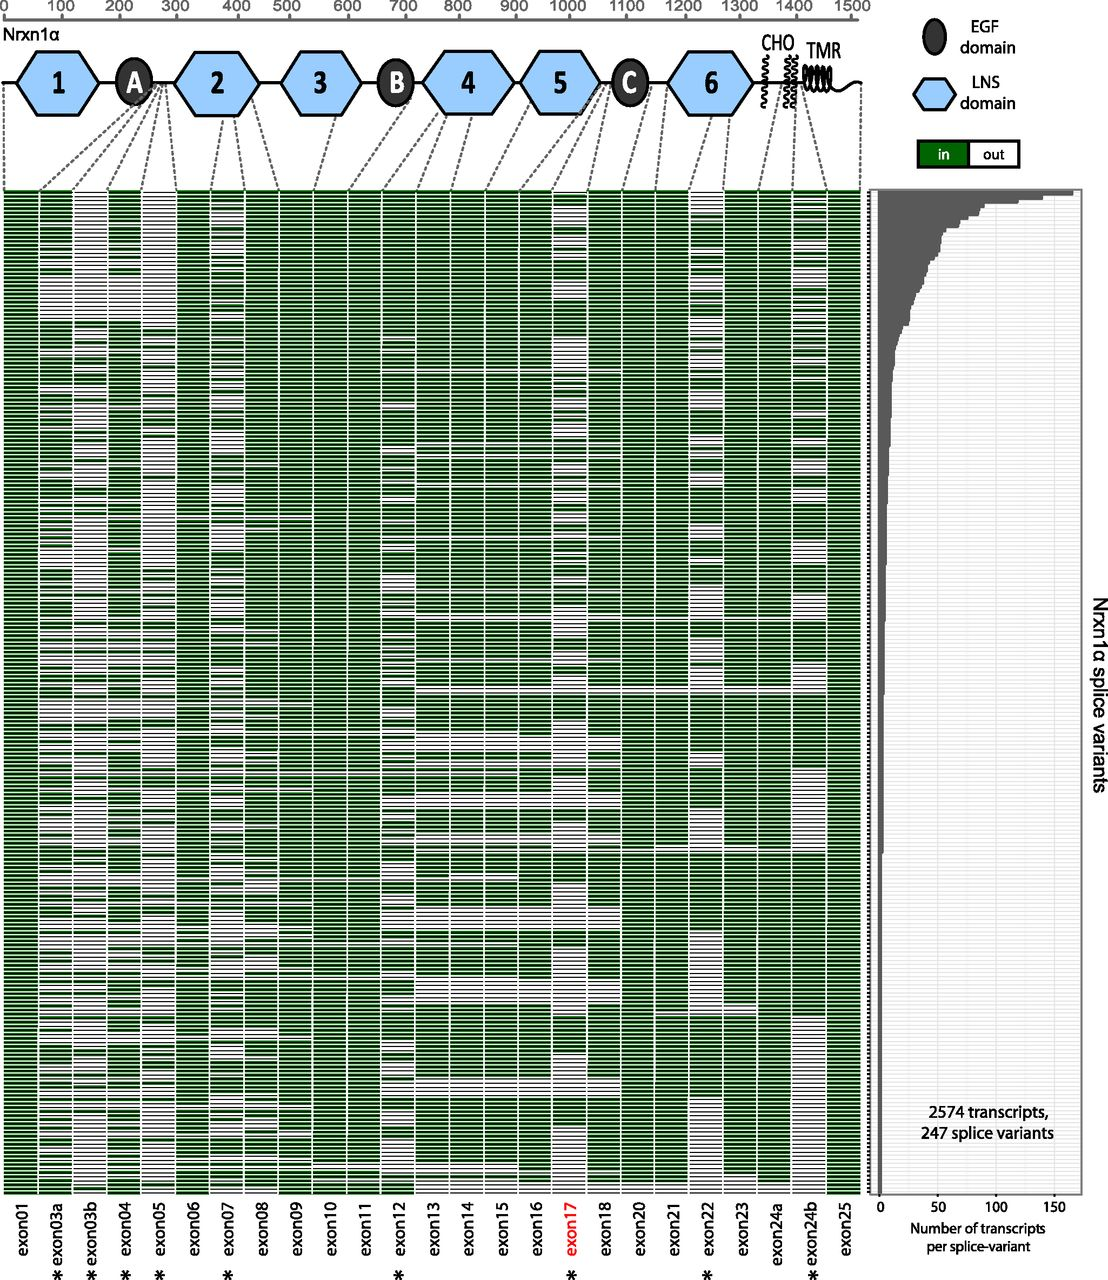
\includegraphics[width=0.6\linewidth]{slides/neurexin_isoforms.jpg}
  \caption{Splice isoforms of mouse neurexin 1$\alpha$ (\textit{Nrxn1}$\alpha$) observed by single-molecule long-read sequencing of full-length mRNAs. Rows are the 247 distinct isoforms and columns are exons, coloured green if included; the bar graph on the right gives the number of transcripts observed for each isoform, and the protein domains encoded by the exons are shown at the top. Reproduced from \citet{treutlein2014}.}
  \label{fig:neurexin}
\end{figure}

%======================================================================
\section{A generative model for RNA-seq reads}
\label{sec:generative}
%======================================================================

\subsection{The model}

Most isoform quantification methods use a variant of the following generative model~\citep{glaus2012,nariai2013,hensman2015}. Let $N$ be the number of reads and $M$ the number of isoforms, indexed by $n\in\{1,\dots,N\}$ and $m\in\{1,\dots,M\}$. In a whole transcriptome $M$ is of the order of $10^5$, since the roughly 20,000 human protein-coding genes have several annotated isoforms each, and $N$ is tens of millions. Let $\vtheta=(\theta_1,\dots,\theta_M)$ be a probability vector, $\theta_m\geq 0$ and $\sum_m\theta_m=1$, where $\theta_m$ is the probability that a randomly chosen read comes from isoform $m$. Let $t_n\in\{1,\dots,M\}$ be the isoform that read $n$ came from, and $r_n$ the observed read (its sequence and alignment). The model is
\begin{align}
  \vtheta &\sim \Dir(\valpha), \nonumber\\
  t_n\mid\vtheta &\sim \Disc(\vtheta), \qquad n=1,\dots,N, \label{eq:genmodel}\\
  r_n\mid t_n &\sim p(r_n\mid t_n), \nonumber
\end{align}
where $\valpha\in\R_{>0}^M$ is the parameter of a Dirichlet prior (Section~\ref{sec:dirichlet}) and $\Disc(\vtheta)$ is the discrete (categorical) distribution with $p(t_n=m\mid\vtheta)=\theta_m$. The prior encodes the intuition that an isoform that makes up more of the RNA is, a priori, more likely to be the source of any given read.

The last line is the \emph{read likelihood}. We do not model the read sequence in detail. Instead, we write $p_{nm}=p(r_n\mid t_n=m)$ for the probability of observing exactly read $n$ given that it came from isoform $m$. In the simplest version, a read of length $l$ is equally likely to start at any position of the isoform, and isoform $m$, of length $L_m$, has
\begin{equation}
  \tilde L_m = L_m - l + 1
\end{equation}
possible start positions: place the read at the start of the isoform and slide it one position at a time until it reaches the end. $\tilde L_m$ is called the \emph{effective length}. If read $n$ aligns to isoform $m$ at one of these positions, it is one of $\tilde L_m$ equally likely reads, so
\begin{equation}
  p_{nm} = \frac{y_{nm}}{\tilde L_m}, \qquad
  y_{nm} = \begin{cases} 1 & \text{if read $n$ is compatible with isoform $m$},\\ 0 & \text{otherwise}. \end{cases}
  \label{eq:readlik}
\end{equation}
The values $p_{nm}$ are computed once from the alignments and stay fixed; only $\vtheta$ and the $t_n$ are unknown. Practical methods refine~\eqref{eq:readlik} with the distribution of fragment lengths for paired-end reads, sequencing error probabilities, and biases in where fragments start along the transcript~\citep{li2011rsem,glaus2012,patro2017}, but these only change the values of $p_{nm}$.

Because a long isoform yields more reads than a short one present in the same number of copies, $\theta_m$ is the share of \emph{reads}, not of molecules. If $\tau_m$ is the fraction of RNA molecules that are isoform $m$, then $\theta_m\propto\tau_m\tilde L_m$, and conversely
\begin{equation}
  \tau_m = \frac{\theta_m/\tilde L_m}{\sum_{m'}\theta_{m'}/\tilde L_{m'}} .
\end{equation}
Multiplying $\tau_m$ by $10^6$ gives the familiar unit of transcripts per million (TPM).

\paragraph{Indicator notation.} It helps to encode $t_n$ as a one-hot vector $\vz_n\in\{0,1\}^M$ with $z_{nm}=\ind[t_n=m]$, where $\ind[\cdot]$ is the indicator function, so that $\sum_m z_{nm}=1$. Then $p(t_n\mid\vtheta)=\theta_{t_n}=\prod_m\theta_m^{z_{nm}}$. The product picks out the right element because $\theta^0=1$ and $\theta^1=\theta$: every factor except the one for $m=t_n$ equals one. Similarly $p(r_n\mid t_n)=p_{nt_n}=\prod_m p_{nm}^{z_{nm}}$. Writing $\mZ\in\{0,1\}^{N\times M}$ for the matrix with rows $\vz_n^\top$ and $R=\{r_1,\dots,r_N\}$ for the reads, the joint distribution of all variables is the product of the three terms of~\eqref{eq:genmodel},
\begin{equation}
  p(\vtheta,\mZ,R) = \underbrace{\frac{\Gamma(\alpha_\cdot)}{\prod_m\Gamma(\alpha_m)}\prod_{m=1}^M\theta_m^{\alpha_m-1}}_{\text{Dirichlet prior}}\;
  \underbrace{\prod_{n=1}^N\prod_{m=1}^M\theta_m^{z_{nm}}}_{\text{read origins}}\;
  \underbrace{\prod_{n=1}^N\prod_{m=1}^M p_{nm}^{z_{nm}}}_{\text{read likelihood}},
  \label{eq:joint}
\end{equation}
where $\Gamma$ is the gamma function and $\alpha_\cdot=\sum_m\alpha_m$.

\subsection{The Dirichlet distribution}
\label{sec:dirichlet}

The Dirichlet distribution is the standard distribution over probability vectors, in the way the Gaussian is the standard distribution over real vectors. For $K$ categories, its random variable is a vector $\vpi\in\R^K$ in the \emph{probability simplex}
\begin{equation}
  \simplex^{K-1} = \Big\{\vpi\in\R^K : \pi_k\geq 0,\ \textstyle\sum_{k=1}^K\pi_k=1\Big\},
\end{equation}
which has dimension $K-1$ because of the sum constraint. Its parameter is a vector $\va\in\R_{>0}^K$, and its density is
\begin{equation}
  \Dir(\vpi;\va) = \frac{\Gamma(a_\cdot)}{\prod_{k=1}^K\Gamma(a_k)}\prod_{k=1}^K\pi_k^{a_k-1}, \qquad a_\cdot=\sum_{k=1}^K a_k ,
  \label{eq:dirichlet}
\end{equation}
where the dot subscript denotes a sum over the index. The ratio of gamma functions is the normalizing constant; the dependence on $\vpi$ is the simple product $\prod_k\pi_k^{a_k-1}$. For $K=2$ the Dirichlet is the beta distribution. Its main properties are:
\begin{itemize}
  \item mean $\E[\pi_k]=a_k/a_\cdot$, the normalized parameter vector;
  \item mode $(a_k-1)/(a_\cdot-K)$, the normalized vector $\va-\mathbf{1}$, provided all $a_k>1$;
  \item variance $\operatorname{Var}[\pi_k]=\dfrac{a_k(a_\cdot-a_k)}{a_\cdot^2(a_\cdot+1)}$;
  \item $\E[\log\pi_k]=\psi(a_k)-\psi(a_\cdot)$, where $\psi(x)=\frac{d}{dx}\log\Gamma(x)$ is the digamma function.
\end{itemize}
The mean suggests a second parameterization, $\va=c\vp$, where $\vp\in\simplex^{K-1}$ is the mean and the scalar $c=a_\cdot>0$ is the \emph{concentration}. The variance becomes $p_k(1-p_k)/(c+1)$, so larger $c$ concentrates the distribution around its mean.

Figure~\ref{fig:dirichlet_simplex} shows Dirichlet densities for $K=3$. The simplex $\simplex^2$ is a triangle in $\R^3$ with corners at $(1,0,0)$, $(0,1,0)$ and $(0,0,1)$; we view it face on, and the distance from a point to each edge is the corresponding component. With $\va=(1,1,1)$, that is $c=3$ and $\vp=(\frac13,\frac13,\frac13)$, the density is uniform. Increasing $c$ concentrates the mass around the centre, and changing $\vp$ moves it. Figure~\ref{fig:dirichlet_draws} shows draws for $K=10$. With $c=100$ a draw is close to its mean; with $c=3$ it is far from it, and many components are close to zero. When some $a_k<1$ (for a uniform mean, when $c<K$), the density becomes infinite at the edges of the simplex and draws are sparse, with most of their mass on a few components.

\begin{figure}[!htbp]
  \centering
  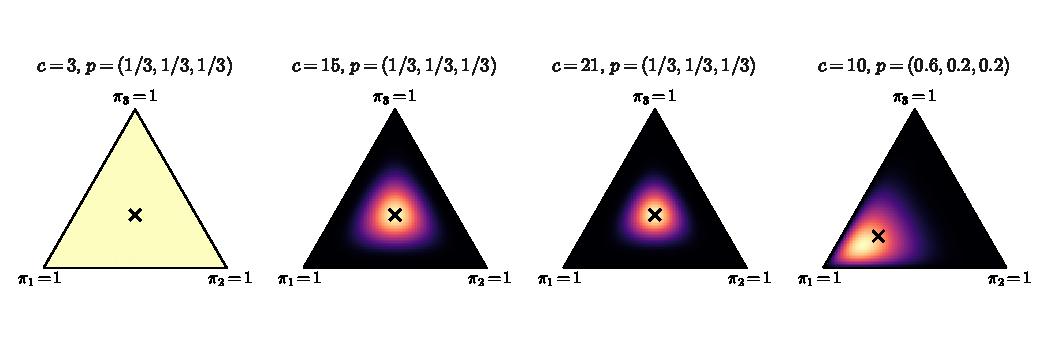
\includegraphics[width=0.95\linewidth]{dirichlet_simplex.pdf}
  \caption{Dirichlet densities on the simplex $\simplex^2$, viewed face on, for parameter $\va=c\vp$. The first three panels have mean $\vp=(\frac13,\frac13,\frac13)$ (cross) and increasing concentration $c$; $c=3$ gives the uniform distribution. The last has mean $(0.6,0.2,0.2)$, nearest the corner where $\pi_1=1$. Lighter colours indicate higher density.}
  \label{fig:dirichlet_simplex}
\end{figure}

\begin{figure}[!htbp]
  \centering
  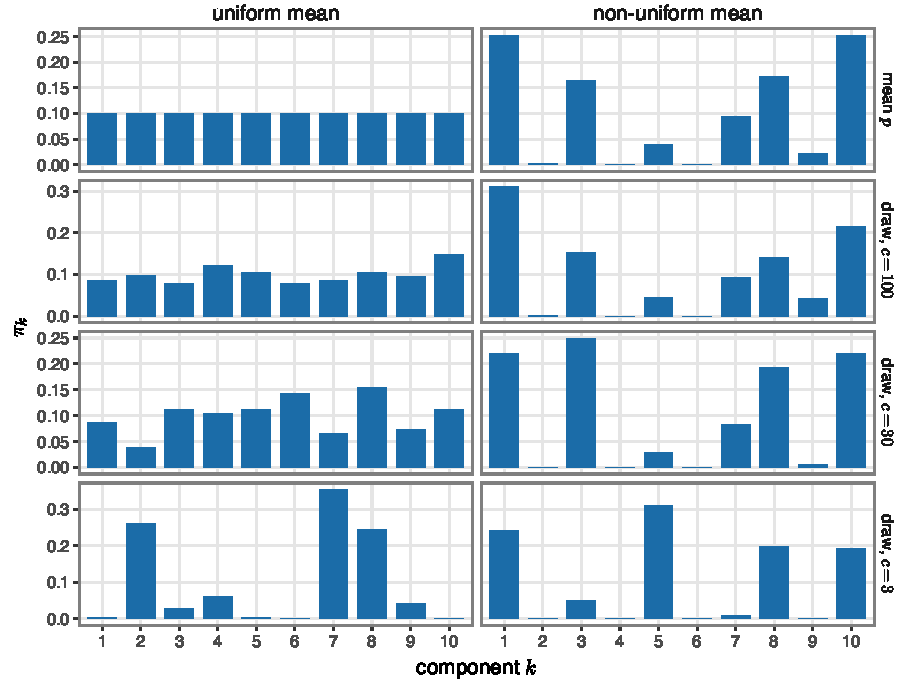
\includegraphics[width=0.95\linewidth]{dirichlet_draws.pdf}
  \caption{Single draws from $\Dir(c\vp)$ with $K=10$, for a uniform mean (left) and a non-uniform mean (right, top row), at concentrations $c=100$, 30 and 3. As $c$ decreases, draws move further from the mean and become sparse.}
  \label{fig:dirichlet_draws}
\end{figure}

The Dirichlet is the \emph{conjugate prior} of the discrete distribution: if $\vpi\sim\Dir(\va)$ and we observe $n_k$ draws of category $k$ from $\Disc(\vpi)$, the posterior is $\Dir(\va+\mathbf{n})$, where $\mathbf{n}=(n_1,\dots,n_K)$. This follows from multiplying~\eqref{eq:dirichlet} by the likelihood $\prod_k\pi_k^{n_k}$, which gives $\prod_k\pi_k^{a_k+n_k-1}$. The parameter $a_k$ therefore acts as a pseudo-count, and $\va=\mathbf{1}$ adds no pseudo-counts at all. In the isoform model, if we knew the read origins $\mZ$, the posterior of $\vtheta$ would be $\Dir(\valpha+\sum_n\vz_n)$. Conjugacy will make every update in the next two sections available in closed form.

\subsection{Graphical model}

Figure~\ref{fig:graphical_model-10} shows the model as a directed graphical model, a notation we used for hidden Markov models in Chapter 6. Each node is a random variable, an edge means that the distribution of the child depends on the parent, and shaded nodes are observed. The rectangles are \emph{plates}: the variables inside a plate are repeated the number of times shown in its corner, like the body of a for loop, and plates can be nested like nested loops. There is one $z_{nm}$ for every read and every isoform, $N\times M$ in total, and one observed read $r_n$ per read. Each $z_{nm}$ depends on $\vtheta$, and each $r_n$ depends on $\vz_n$.

\begin{figure}[!htbp]
  \centering
  \begin{tikzpicture}[>=Stealth, every node/.style={font=\small},
      var/.style={circle, draw, minimum size=0.9cm}, obs/.style={var, fill=gray!25}]
    \node[var] (alpha) at (-2.0,0) {$\valpha$};
    \node[var] (theta) at (0,0) {$\vtheta$};
    \node[var] (z) at (2.8,0) {$z_{nm}$};
    \node[obs] (r) at (2.8,-2.0) {$r_n$};
    \draw[->] (alpha) -- (theta);
    \draw[->] (theta) -- (z);
    \draw[->] (z) -- (r);
    \node[draw, rounded corners, fit=(z), inner sep=0.35cm, label={[anchor=south east]south east:$M$}] (pm) {};
    \node[draw, rounded corners, fit=(pm)(r), inner sep=0.3cm, label={[anchor=south east]south east:$N$}] {};
  \end{tikzpicture}
  \caption{Graphical model for isoform quantification, adapted from \citet{hensman2015}. Plates denote repetition over isoforms $m$ and reads $n$; the shaded node is observed. The quantity of interest is the posterior $p(\vtheta\mid R)$.}
  \label{fig:graphical_model-10}
\end{figure}

What we would like is the posterior $p(\vtheta\mid R)$. Obtaining it requires summing the joint~\eqref{eq:joint} over the latent assignments $\mZ$. The sum over the assignment of each read is easy, but the posterior over $\vtheta$ that results, $p(\vtheta\mid R)\propto\Dir(\vtheta;\valpha)\prod_n\sum_m\theta_m p_{nm}$, is a product of $N$ sums. Expanding it gives a mixture of up to $M^N$ Dirichlet distributions, one per joint assignment of reads to isoforms, which cannot be computed. We consider two ways around this: point estimation of $\vtheta$ by EM, and approximation of the full posterior by variational inference.

%======================================================================
\section{EM for isoform abundance}
\label{sec:em-10}
%======================================================================

EM was derived in Chapter 5 for mixture models and used in Chapter 6 for hidden Markov models. It maximizes a lower bound on the log marginal probability of the data by alternating two steps: the E step sets a distribution $q(\mZ)$ over the latent variables to their posterior given the current parameters, and the M step maximizes the expected log joint probability under $q$ over the parameters. Here the latent variables are the read assignments $\mZ$ and the parameter is $\vtheta$. Because we keep the Dirichlet prior, the M step maximizes the expected log \emph{posterior} and EM finds a maximum a posteriori (MAP) estimate of $\vtheta$; with $\valpha=\mathbf{1}$ the prior is flat and the estimate is the maximum likelihood estimate.

\subsection{E step}

The E step computes the posterior over the assignments given the current $\vtheta$. Only the second and third factors of~\eqref{eq:joint} involve $\mZ$, and they factorize over reads, so the assignments of different reads are independent given $\vtheta$ and
\begin{equation}
  q(\vz_n) = p(\vz_n\mid r_n,\vtheta) \propto \prod_{m=1}^M\theta_m^{z_{nm}}p_{nm}^{z_{nm}} = \prod_{m=1}^M\left(\theta_m p_{nm}\right)^{z_{nm}} .
\end{equation}
This is the probability mass function of a discrete distribution over which entry of $\vz_n$ equals one, with unnormalized probabilities $\phi^*_{nm}=\theta_m p_{nm}$. Normalizing,
\begin{equation}
  q(\vz_n) = \prod_{m=1}^M\phi_{nm}^{z_{nm}}, \qquad
  \phi_{nm} = \frac{\theta_m p_{nm}}{\sum_{m'=1}^M\theta_{m'}p_{nm'}} ,
  \label{eq:estep}
\end{equation}
where $\phi_{nm}\in[0,1]$, with $\sum_m\phi_{nm}=1$, is the posterior probability that read $n$ came from isoform $m$, also called its \emph{responsibility}. The general pattern is worth noting. Collect the terms of the joint that involve the variable of interest, recognize the result as the unnormalized form of a standard distribution, and read off its parameters. The same pattern recurs in the M step and in variational inference.

\subsection{M step}

The M step maximizes the expected log joint under $q(\mZ)=\prod_n q(\vz_n)$. Taking the log of~\eqref{eq:joint},
\begin{equation}
  \log p(\vtheta,\mZ,R) = \sum_{m=1}^M(\alpha_m-1)\log\theta_m + \sum_{n=1}^N\sum_{m=1}^M z_{nm}\log\theta_m + \sum_{n=1}^N\sum_{m=1}^M z_{nm}\log p_{nm} + \text{const},
\end{equation}
where the constant is the log normalizer of the Dirichlet, which does not involve $\vtheta$. Expectation is linear, so it moves inside the sums, and $\E_q[z_{nm}]=\phi_{nm}$ because $z_{nm}$ is one with probability $\phi_{nm}$ and zero otherwise. Dropping terms that do not involve $\vtheta$ and exchanging the order of the sums over $n$ and $m$,
\begin{equation}
  \E_q\left[\log p(\vtheta,\mZ,R)\right] = \sum_{m=1}^M\Big(\alpha_m-1+\sum_{n=1}^N\phi_{nm}\Big)\log\theta_m + \text{const}
  = \sum_{m=1}^M(\alpha'_m-1)\log\theta_m + \text{const},
\end{equation}
with
\begin{equation}
  \alpha'_m = \alpha_m + \sum_{n=1}^N\phi_{nm} .
  \label{eq:alphaprime}
\end{equation}
Up to a constant this is the log density of $\Dir(\vtheta;\valpha')$, so the M step returns its mode. To derive the mode, maximize $\sum_m(\alpha'_m-1)\log\theta_m$ subject to $\sum_m\theta_m=1$ with a Lagrange multiplier $\lambda$. Setting the derivative of $\sum_m(\alpha'_m-1)\log\theta_m-\lambda(\sum_m\theta_m-1)$ with respect to $\theta_m$ to zero gives $(\alpha'_m-1)/\theta_m=\lambda$, so $\theta_m=(\alpha'_m-1)/\lambda$, and the constraint gives $\lambda=\sum_m(\alpha'_m-1)=\alpha_\cdot-M+N$, using $\sum_n\sum_m\phi_{nm}=N$. The M step is therefore
\begin{equation}
  \theta_m^{\text{new}} = \frac{\alpha'_m-1}{\alpha'_\cdot-M} = \frac{\alpha_m-1+\sum_n\phi_{nm}}{N+\alpha_\cdot-M},
  \label{eq:mstep-10}
\end{equation}
which requires $\alpha'_m\geq 1$; for $\alpha_m<1$ the maximum can lie on the boundary $\theta_m=0$. With a flat prior, $\valpha=\mathbf{1}$, the update is $\theta_m^{\text{new}}=\frac{1}{N}\sum_n\phi_{nm}$.

The quantity $\sum_n\phi_{nm}$ is the \emph{expected count} of reads from isoform $m$, the analogue of the expected number of points in a cluster in EM for a Gaussian mixture. The algorithm alternates between dividing each read among the isoforms it is compatible with, in proportion to their current abundances weighted by $1/\tilde L_m$, and re-estimating the abundances from the resulting fractional counts (Algorithm~\ref{alg:em}).

\begin{algorithm}[!htbp]
  \caption{EM for isoform abundance}
  \label{alg:em}
  \begin{algorithmic}[1]
    \State Compute $p_{nm}=y_{nm}/\tilde L_m$ from the read alignments
    \State Initialize $\theta_m\gets 1/M$ for all $m$
    \Repeat
      \State E step: $\phi_{nm}\gets\theta_m p_{nm}/\sum_{m'}\theta_{m'}p_{nm'}$ for all $n,m$
      \State M step: $\theta_m\gets(\alpha_m-1+\sum_n\phi_{nm})/(N+\alpha_\cdot-M)$ for all $m$
    \Until{the log posterior $\log\Dir(\vtheta;\valpha)+\sum_n\log\sum_m\theta_m p_{nm}$ stops increasing}
    \State Return $\vtheta$, and $\tau_m\propto\theta_m/\tilde L_m$
  \end{algorithmic}
\end{algorithm}

\subsection{Properties}

As shown in Chapter 5, each EM iteration cannot decrease the objective, here the log posterior
\begin{equation}
  \log p(\vtheta\mid R) = \sum_{m=1}^M(\alpha_m-1)\log\theta_m + \sum_{n=1}^N\log\sum_{m=1}^M\theta_m p_{nm} + \text{const}.
\end{equation}
Unlike the Gaussian mixture, this objective is concave in $\vtheta$ when $\valpha\geq\mathbf{1}$: each $\sum_m\theta_m p_{nm}$ is linear in $\vtheta$, the logarithm of a linear function is concave, sums of concave functions are concave, and the simplex is convex. EM therefore converges to a global maximum, although it can be slow when isoforms are hard to distinguish, and the maximum need not be unique. If two isoforms are compatible with exactly the same reads, for example, only their combined abundance is determined by the data.

The E step depends on a read only through its vector $(p_{n1},\dots,p_{nM})$, which by~\eqref{eq:readlik} is determined by the set of isoforms the read is compatible with. Reads with the same compatibility set, an \emph{equivalence class}, have identical responsibilities, so the E step can be computed once per class and weighted by the number of reads in it. Fast methods such as kallisto~\citep{bray2016} and salmon~\citep{patro2017} exploit this, together with fast approximate alignment (pseudoalignment), to quantify tens of millions of reads in minutes.

Figure~\ref{fig:em_toy} runs EM on a simulated gene with the three-isoform structure of Figure~\ref{fig:read_ambiguity}. Starting from uniform abundances, the estimates converge within a few tens of iterations to the maximum likelihood estimate, which is close to the values used to simulate the data, and the log likelihood increases at every iteration.

\begin{figure}[!htbp]
  \centering
  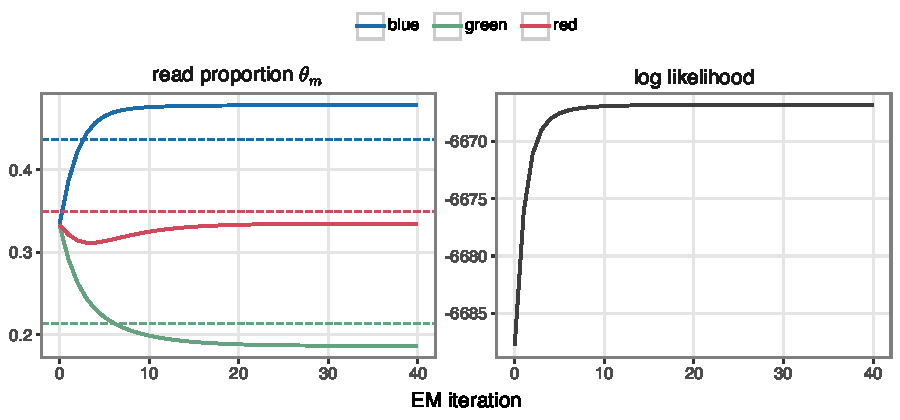
\includegraphics[width=0.9\linewidth]{em_toy.pdf}
  \caption{EM for a simulated three-isoform gene with the structure of Figure~\ref{fig:read_ambiguity} ($N=1000$ reads of length $l=50$, flat prior). Left: estimated read proportions $\theta_m$ by iteration, with the values used to simulate the data dashed. Right: the log likelihood $\sum_n\log\sum_m\theta_m p_{nm}$ never decreases.}
  \label{fig:em_toy}
\end{figure}

%======================================================================
\section{Variational Bayesian inference}
\label{sec:vi}
%======================================================================

EM keeps a distribution over the read assignments $\mZ$, so it represents our uncertainty about which isoform each read came from, but it returns a single value of $\vtheta$. That can be misleading. An isoform supported by only a handful of reads, or one that can be distinguished from another only through a few junction reads, has an abundance we know poorly, and a point estimate does not say so. The Bayesian answer is the posterior $p(\vtheta\mid R)$, which we saw is intractable. \emph{Variational inference} approximates it: we choose a family of tractable distributions $q$ and find the member closest to the posterior. It replaces a hard integration problem with an optimization problem, which is usually easier in high dimensions.

\subsection{The evidence lower bound}

Consider a general model with latent variables $\vz$ (which may include parameters) and data $\vx$. By Bayes' rule the posterior is
\begin{equation}
  p(\vz\mid\vx) = \frac{p(\vx\mid\vz)\,p(\vz)}{p(\vx)} = \frac{f(\vz)}{C},
\end{equation}
where $f(\vz)=p(\vx,\vz)$ is the joint probability, which we can evaluate, and $C=p(\vx)=\int f(\vz)\,d\vz$ is the evidence or marginal likelihood, which we cannot. For any distribution $q(\vz)$, multiplying and dividing by $q$ inside the integral and applying Jensen's inequality to the concave logarithm, as in Chapter 5,
\begin{equation}
  \log C = \log\int q(\vz)\frac{f(\vz)}{q(\vz)}\,d\vz \geq \int q(\vz)\log\frac{f(\vz)}{q(\vz)}\,d\vz \equiv \mathcal{F}[q] .
\end{equation}
$\mathcal{F}[q]$ is the evidence lower bound (ELBO), or variational free energy. The gap is
\begin{equation}
  \log C - \mathcal{F}[q] = \int q(\vz)\left[\log C + \log\frac{q(\vz)}{f(\vz)}\right]d\vz = \int q(\vz)\log\frac{q(\vz)}{p(\vz\mid\vx)}\,d\vz = \KL\big(q\,\|\,p(\cdot\mid\vx)\big),
  \label{eq:vi_gap}
\end{equation}
using $\int q=1$ and $f/C=p(\vz\mid\vx)$. The Kullback-Leibler (KL) divergence $\KL(q\|p)=\int q\log(q/p)$ is non-negative and zero only when $q=p$. Since $\log C$ does not depend on $q$, maximizing $\mathcal{F}[q]$ over $q$ is the same as minimizing the KL divergence from $q$ to the posterior, and it requires only the joint $f$, not the evidence. EM is the special case in which $q$ is unrestricted over the latent variables and a point mass over the parameters.

\subsection{Which divergence?}

The KL divergence is not symmetric, and the direction matters. $\KL(q\|p)$ averages $\log(q/p)$ under $q$. Where $p$ is close to zero and $q$ is not, $\log(q/p)$ is very large, so the optimal $q$ avoids putting mass where the posterior has none. This is called \emph{zero forcing}. As a result, $q$ tends to fit one mode of a multimodal $p$ and ignore the others, which is called \emph{mode seeking}, and it tends to underestimate the spread of $p$. The reverse divergence $\KL(p\|q)$ penalizes $q$ for missing mass that $p$ has, so it spreads $q$ to cover all of $p$; for a Gaussian $q$ it matches the mean and variance of $p$. \citet{minka2005} placed both in the family of $\alpha$-divergences,
\begin{equation}
  D_\alpha(p\,\|\,q) = \frac{1}{\alpha(1-\alpha)}\int\left[\alpha p(\vz)+(1-\alpha)q(\vz)-p(\vz)^\alpha q(\vz)^{1-\alpha}\right]d\vz,
\end{equation}
which tends to $\KL(q\|p)$ as $\alpha\to 0$ and to $\KL(p\|q)$ as $\alpha\to 1$, with intermediate values interpolating between zero forcing and mass covering (Figure~\ref{fig:kl_directions}). Standard variational inference uses $\KL(q\|p)$, the one direction in which the expectation is under the tractable $q$; expectation propagation uses the other.

\begin{figure}[!htbp]
  \centering
  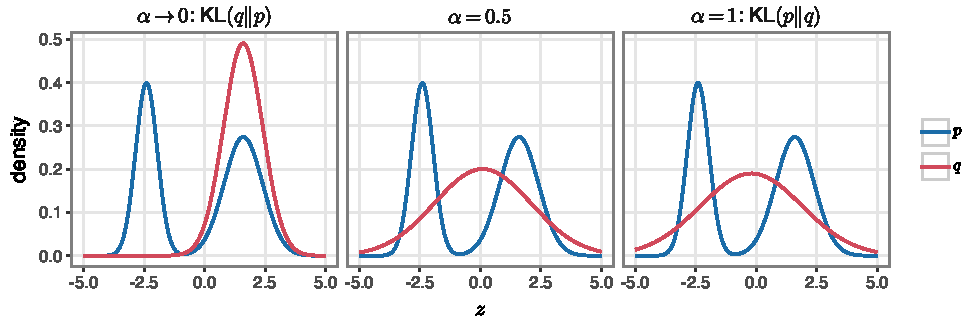
\includegraphics[width=0.95\linewidth]{kl_directions.pdf}
  \caption{The Gaussian $q$ (red) that minimizes the $\alpha$-divergence $D_\alpha(p\|q)$ to a bimodal $p$ (blue), found numerically. $\alpha\to0$ gives $\KL(q\|p)$, used by variational inference, which locks onto one mode (zero forcing); $\alpha=1$ gives $\KL(p\|q)$, which matches the mean and variance of $p$ and covers both modes.}
  \label{fig:kl_directions}
\end{figure}

\subsection{Mean-field approximation and coordinate ascent}

The family of approximating distributions must be simple enough that $\mathcal{F}[q]$ can be computed. In \emph{mean-field} variational inference (the name comes from statistical physics) we assume $q$ factorizes over groups of variables,
\begin{equation}
  q(\vz) = \prod_{i=1}^I q_i(\vz_i),
\end{equation}
where $\vz_1,\dots,\vz_I$ partition $\vz$, and we make no other assumption about the form of the factors. The true posterior has dependencies between the groups; in the isoform model, for instance, the components of $\vtheta$ must sum to one, so if one is larger the others must be smaller. The factorized $q$ ignores such dependencies.

The factors can be optimized one at a time, holding the others fixed. Write $q_{-i}=\prod_{j\neq i}q_j$ and $\E_{-i}$ for expectation under $q_{-i}$. Separating the terms of $\mathcal{F}$ that involve $q_i$,
\begin{equation}
  \mathcal{F}[q] = \int q_i(\vz_i)\,\E_{-i}\left[\log f(\vz)\right]d\vz_i - \int q_i(\vz_i)\log q_i(\vz_i)\,d\vz_i + \text{const},
\end{equation}
where the constant collects the entropies of the other factors. Define the distribution
\begin{equation}
  \tilde p_i(\vz_i) = \frac{1}{Z_i}\exp\E_{-i}\left[\log f(\vz)\right],
\end{equation}
where $Z_i$ is its normalizing constant. Then the first two terms equal $-\KL(q_i\|\tilde p_i)+\log Z_i$, which is maximized by $q_i=\tilde p_i$. This gives the \emph{coordinate ascent variational inference} (CAVI) update~\citep{blei2017}, also known as variational Bayes EM,
\begin{equation}
  q_i^{\text{new}}(\vz_i) \propto \exp\left(\int\log f(\vz)\prod_{j\neq i}q_j(\vz_j)\,d\vz_{-i}\right) = \exp\,\E_{-i}\left[\log p(\vx,\vz)\right].
  \label{eq:cavi}
\end{equation}
Cycling through the factors increases $\mathcal{F}$ at every step, so CAVI converges to a local maximum of the ELBO.

\subsection{CAVI for isoform abundance}

For the isoform model we treat both $\vtheta$ and $\mZ$ as unknowns and assume
\begin{equation}
  q(\vtheta,\mZ) = q(\vtheta)\prod_{n=1}^N q(\vz_n),
\end{equation}
that is, abundances independent of assignments, and assignments of different reads independent of each other. Given $\vtheta$ the reads are independent anyway, so the only approximation is the independence of $\vtheta$ and $\mZ$.

\paragraph{Update for $q(\vz_n)$.} The terms of the log joint $\log p(\vtheta,\mZ,R)$ that involve $\vz_n$ are $\sum_m z_{nm}(\log\theta_m+\log p_{nm})$, so by~\eqref{eq:cavi}
\begin{equation}
  q^{\text{new}}(\vz_n) \propto \exp\,\E_{q(\vtheta)}\Big[\sum_{m=1}^M z_{nm}\log\theta_m + z_{nm}\log p_{nm}\Big] = \prod_{m=1}^M\left(p_{nm}e^{\E[\log\theta_m]}\right)^{z_{nm}},
\end{equation}
a discrete distribution, $q(\vz_n)=\prod_m\phi_{nm}^{z_{nm}}$, with
\begin{equation}
  \phi_{nm} = \frac{p_{nm}\exp(\E_{q(\vtheta)}[\log\theta_m])}{\sum_{m'}p_{nm'}\exp(\E_{q(\vtheta)}[\log\theta_{m'}])} .
  \label{eq:vb_phi}
\end{equation}
This is the E step~\eqref{eq:estep} with $\theta_m$ replaced by $\exp\E[\log\theta_m]$.

\paragraph{Update for $q(\vtheta)$.} The terms involving $\vtheta$ are the Dirichlet prior and the read origins. Taking the expectation under $q(\mZ)$, with $\E[z_{nm}]=\phi_{nm}$,
\begin{equation}
  q^{\text{new}}(\vtheta) \propto \exp\,\E_{q(\mZ)}\Big[\sum_m(\alpha_m-1)\log\theta_m + \sum_n\sum_m z_{nm}\log\theta_m\Big] = \prod_{m=1}^M\theta_m^{\alpha'_m-1},
\end{equation}
with $\alpha'_m=\alpha_m+\sum_n\phi_{nm}$ as in~\eqref{eq:alphaprime}. This is the kernel of a Dirichlet, so $q(\vtheta)=\Dir(\vtheta;\valpha')$. The computation is the same as in the M step; the only difference is that we exponentiate rather than maximize, and so keep the whole distribution rather than its mode. The expectation needed in~\eqref{eq:vb_phi} then has a closed form,
\begin{equation}
  \E_{q(\vtheta)}[\log\theta_m] = \psi(\alpha'_m) - \psi(\alpha'_\cdot).
\end{equation}

We assumed only the factorization. That $q(\vz_n)$ came out discrete and $q(\vtheta)$ came out Dirichlet was not assumed: it follows from~\eqref{eq:cavi} because the Dirichlet prior is conjugate to the discrete distribution of the read origins. The model is \emph{conditionally conjugate}: each variable's conditional distribution given the others is in the same family as its prior.

Algorithm~\ref{alg:cavi} collects the updates. Convergence can be monitored with the ELBO. Substituting the factors into $\mathcal{F}=\E_q[\log p(\vtheta,\mZ,R)]-\E_q[\log q(\vtheta)]-\sum_n\E_q[\log q(\vz_n)]$, the terms in $\E[\log\theta_m]$ cancel once $\valpha'=\valpha+\sum_n\vphi_n$, leaving
\begin{equation}
  \mathcal{F} = \log\frac{\Gamma(\alpha_\cdot)}{\Gamma(\alpha'_\cdot)} + \sum_{m=1}^M\log\frac{\Gamma(\alpha'_m)}{\Gamma(\alpha_m)} + \sum_{n=1}^N\sum_{m=1}^M\phi_{nm}\log\frac{p_{nm}}{\phi_{nm}} .
\end{equation}

\begin{algorithm}[!htbp]
  \caption{CAVI for isoform abundance}
  \label{alg:cavi}
  \begin{algorithmic}[1]
    \State Compute $p_{nm}$ from the alignments; initialize $\valpha'\gets\valpha+N/M$
    \Repeat
      \State $\phi_{nm}\gets p_{nm}\exp(\psi(\alpha'_m)-\psi(\alpha'_\cdot))$, then normalize over $m$, for all $n$
      \State $\alpha'_m\gets\alpha_m+\sum_n\phi_{nm}$ for all $m$
    \Until{the ELBO $\mathcal{F}$ stops increasing}
    \State Return $q(\vtheta)=\Dir(\valpha')$, with posterior mean $\alpha'_m/\alpha'_\cdot$
  \end{algorithmic}
\end{algorithm}

The update has a simple interpretation. For large $x$, $\exp(\psi(x))\approx x-\frac12$, so for well-supported isoforms $\exp\E[\log\theta_m]\approx(\alpha'_m-\frac12)/\alpha'_\cdot$, close to the EM value. For isoforms with small expected counts, $\exp(\psi(x))$ is much smaller than $x$ (it tends to zero as $x\to 0$), so CAVI is less willing than EM to give reads to isoforms that have little support, and it can drive their abundance toward zero.

\subsection{Does it work?}

\citet{hensman2015} implemented this algorithm in BitSeq, which previously sampled the posterior by Markov chain Monte Carlo (MCMC)~\citep{glaus2012}. MCMC draws samples whose distribution converges to the exact posterior; it is the traditional approach to Bayesian inference but is slow and hard to diagnose. They assessed accuracy with technical replicates, in which the same biological sample is sequenced twice, so the true abundances are the same and the mean absolute error between the two estimates measures reproducibility (Figure~\ref{fig:bitseq}). The variational version was slightly less reproducible than MCMC, the cost of the factorization assumption, but better than most other methods and about an order of magnitude faster than MCMC. Kallisto~\citep{bray2016}, which runs EM on equivalence classes after pseudoalignment, was the fastest by far and somewhat less accurate.

\begin{figure}[!htbp]
  \centering
  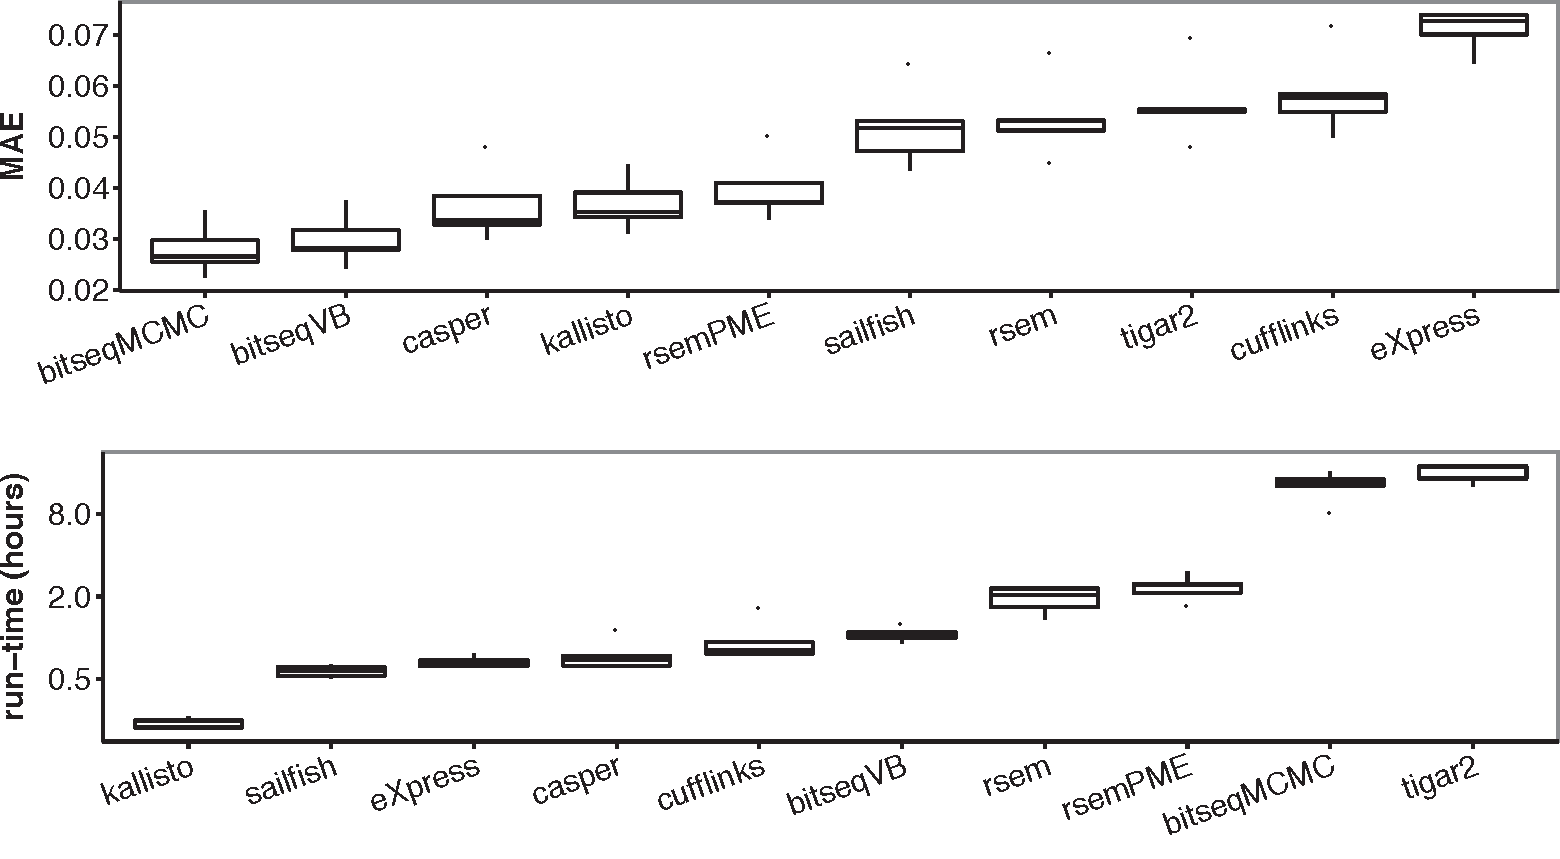
\includegraphics[width=0.8\linewidth]{slides/bitseq_comparison.pdf}
  \caption{Comparison of isoform quantification methods on five pairs of ENCODE technical replicates. Top: mean absolute error (MAE) between estimates from the two replicates. Bottom: run time for about 25 million mapped reads per sample. bitseqVB is the CAVI algorithm of this section; bitseqMCMC samples the same posterior by MCMC. Reproduced from \citet{hensman2015}.}
  \label{fig:bitseq}
\end{figure}

Figure~\ref{fig:vb_vs_gibbs} compares CAVI with the exact posterior, approximated by a long run of Gibbs sampling, on a simulated gene with few reads. The posterior means agree, but the CAVI marginals are narrower than the exact ones: their standard deviations are between about two thirds and three quarters of the exact values.

\begin{figure}[!htbp]
  \centering
  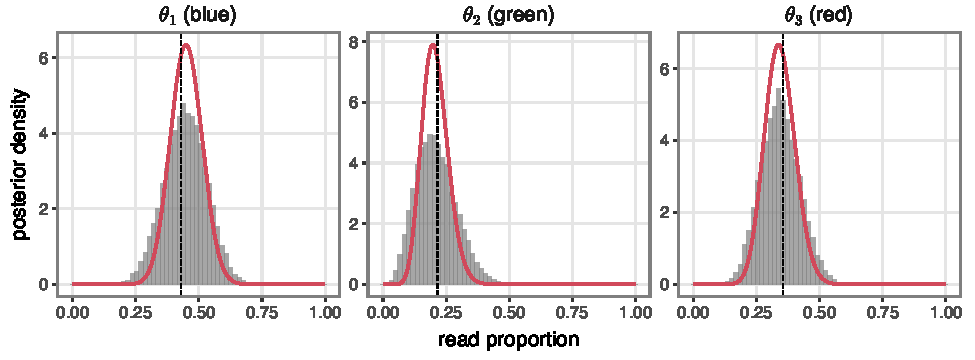
\includegraphics[width=0.95\linewidth]{vb_vs_gibbs.pdf}
  \caption{Posterior marginals of the read proportions $\theta_m$ for a simulated three-isoform gene with $N=60$ reads and $\valpha=\mathbf{1}$: Gibbs sampling, which converges to the exact posterior (histograms, 20,000 samples), and CAVI (lines, the beta marginals of $\Dir(\valpha')$). Dashed lines mark the values used to simulate the data. CAVI recovers the posterior means but underestimates the uncertainty.}
  \label{fig:vb_vs_gibbs}
\end{figure}

\subsection{Limitations of CAVI}

CAVI has three main limitations.
\begin{enumerate}
  \item \emph{It requires conditionally conjugate models.} The updates came out in closed form because the Dirichlet is conjugate to the discrete distribution. With a different prior on $\vtheta$, for example a logistic-normal distribution that could model correlations between isoform abundances, the expectations in~\eqref{eq:cavi} are no longer available in closed form.
  \item \emph{It underestimates posterior variance.} The mean-field factorization combined with the zero-forcing KL divergence makes $q$ too narrow when the posterior has strong dependencies (Figure~\ref{fig:meanfield}). For a Gaussian posterior $\Normal(\vmu,\mLambda^{-1})$ over $\vz\in\R^2$ with precision matrix $\mLambda$, the CAVI update~\eqref{eq:cavi} for $q_1(z_1)$ collects the terms of $-\frac12(\vz-\vmu)^\top\mLambda(\vz-\vmu)$ that involve $z_1$, namely $-\frac12\Lambda_{11}z_1^2+z_1\left(\Lambda_{11}\mu_1-\Lambda_{12}(\E[z_2]-\mu_2)\right)$, which is the log density of a Gaussian with variance $1/\Lambda_{11}$. At the fixed point the means are exact, but $1/\Lambda_{11}=\Sigma_{11}(1-\rho^2)$, where $\mSigma=\mLambda^{-1}$ and $\rho$ is the posterior correlation, so the approximate variance is smaller than the true marginal variance $\Sigma_{11}$ by the factor $1-\rho^2$. The more correlated the posterior, the more uncertainty is lost, which defeats part of the purpose of Bayesian inference.
  \item \emph{It does not scale to large data.} Each update of the global factor $q(\vtheta)$ requires a pass over all $N$ reads, like full-batch rather than stochastic gradient descent.
\end{enumerate}

\begin{figure}[!htbp]
  \centering
  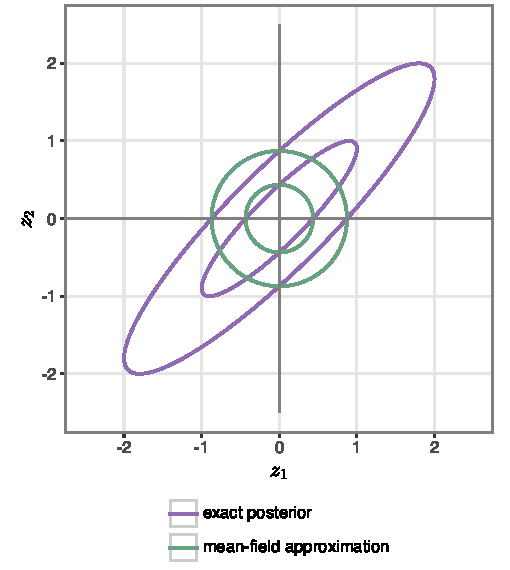
\includegraphics[width=0.5\linewidth]{meanfield.pdf}
  \caption{A correlated Gaussian posterior (purple, correlation $\rho=0.9$) and its mean-field approximation minimizing $\KL(q\|p)$ (green). Contours enclose 39\% and 86\% of the mass (one and two standard deviations). The approximation has the right mean but its variances, $\Sigma_{ii}(1-\rho^2)$, are much smaller than the true marginal variances.}
  \label{fig:meanfield}
\end{figure}

%======================================================================
\section{Stochastic variational inference}
\label{sec:svi}
%======================================================================

Stochastic variational inference addresses all three limitations by applying stochastic gradient methods directly to the KL divergence~\citep{nott2012,paisley2012,salimans2013,hoffman2013,ranganath2014}. It is stochastic in two ways: it uses Monte Carlo samples to approximate the expectations in the objective, which removes the need for conjugacy, and it uses minibatches of data, which makes it scale. It is the basis of the variational autoencoder, which we meet in a later chapter.

\paragraph{Monte Carlo estimation.} For a distribution $q(\vz)$ and a function $g(\vz)$, the expectation $\E_q[g(\vz)]$ can be estimated by drawing $S$ samples $\vz^{(1)},\dots,\vz^{(S)}\sim q$ and averaging,
\begin{equation}
  \E_q[g(\vz)] \approx \frac{1}{S}\sum_{s=1}^S g(\vz^{(s)}).
\end{equation}
The estimate is \emph{unbiased}: its expectation is exactly $\E_q[g(\vz)]$ for any $S$, and its variance decreases as $1/S$. Stochastic gradient descent needs only unbiased estimates of the gradient (Chapter 2), so even $S=1$ suffices.

\paragraph{The reparameterization trick.} Let $q_{\veta}(\vz)$ be a parametric approximation with variational parameters $\veta$, and write $p(\vz)$ for the joint $p(\vx,\vz)$ as a function of $\vz$, which differs from the posterior only by the constant $\log C$. Then
\begin{equation}
  \KL(q_{\veta}\|p) = \int q_{\veta}(\vz)\log q_{\veta}(\vz)\,d\vz - \int q_{\veta}(\vz)\log p(\vz)\,d\vz = -H[q_{\veta}] - \E_{q_{\veta}}[\log p(\vz)],
\end{equation}
where $H[q]=-\int q\log q$ is the entropy, which for common families such as the Gaussian has a closed form. The second term is an expectation under a distribution that depends on $\veta$, so we cannot simply differentiate inside a Monte Carlo average. The trick is to write a draw from $q_{\veta}$ as a deterministic, differentiable function of $\veta$ and of noise $\vu$ drawn from a fixed distribution $\pi_0(\vu)$: $\vz=h(\vu,\veta)$ with $\vu\sim\pi_0$, chosen so that $\vz\sim q_{\veta}$. For example, $z=m+\sqrt{v}\,u$ with $u\sim\Normal(0,1)$ and $\veta=\{m,v\}$ gives $z\sim\Normal(m,v)$. Changing variables,
\begin{equation}
  \KL(q_{\veta}\|p) = -H[q_{\veta}] - \int\pi_0(\vu)\log p(h(\vu,\veta))\,d\vu ,
\end{equation}
and now the distribution under the integral does not depend on $\veta$, so the gradient can move inside it,
\begin{align}
  \nabla_{\veta}\KL &= -\nabla_{\veta}H[q_{\veta}] - \int\pi_0(\vu)\,\nabla_{\veta}\log p(h(\vu,\veta))\,d\vu \nonumber\\
  &\approx -\nabla_{\veta}H[q_{\veta}] - \nabla_{\veta}\log p(h(\vu,\veta)), \qquad \vu\sim\pi_0 .
\end{align}
The single-sample estimate is unbiased, so it can drive stochastic gradient descent, and the gradient $\nabla_{\veta}\log p(h(\vu,\veta))$ is computed by automatic differentiation, as for a neural network. In the Gaussian example, $H=\frac12\log(2\pi e v)$ and, by the chain rule, $\partial\log p/\partial m=\partial\log p/\partial z$ and $\partial\log p/\partial v=(\partial\log p/\partial z)\,u/(2\sqrt v)$.

\paragraph{Minibatches.} When the data are $N$ conditionally independent observations, $\log p(\vx,\vz)=\log p(\vz)+\sum_{n=1}^N\log p(\vx_n\mid\vz)$. Replacing the sum by $\frac{N}{B}$ times the sum over a random minibatch of $B$ observations gives another unbiased estimate, so each gradient step touches only $B$ observations. In the isoform model, the assignment of each read can be summed out exactly, $\log p(r_n\mid\vtheta)=\log\sum_m\theta_m p_{nm}$, and $q(\vtheta)$ could be any distribution on the simplex that can be reparameterized, for example $\vtheta=\operatorname{softmax}(\vmu+\operatorname{diag}(\boldsymbol{\sigma})\vu)$ with $\vu\sim\Normal(\mathbf{0},\mI)$, whose parameters $\vmu,\boldsymbol{\sigma}\in\R^M$ are learned; no conjugacy is required. Probabilistic programming frameworks such as Pyro~\citep{bingham2019}, built on PyTorch, and NumPyro~\citep{phan2019}, built on JAX, automate these steps for models written as programs, including models with neural network components.

%======================================================================
\section{Predicting splicing from sequence}
\label{sec:seq_models}
%======================================================================

\subsection{How splice sites are recognized}

Splicing is carried out and regulated by many proteins and RNAs (Figure~\ref{fig:spliceosome}). The core of the spliceosome is a set of \emph{small nuclear ribonucleoproteins} (snRNPs), each a complex of proteins with a short non-coding RNA. Several of them recognize their targets by base pairing. Early in spliceosome assembly, U1 snRNP binds the $5'$ splice site because the U1 RNA is complementary to the donor consensus; this is a different mechanism from the protein-DNA recognition used by transcription factors. At the other end of the intron, SF1 binds the branch point, the U2AF heterodimer binds the polypyrimidine tract (U2AF65) and the terminal AG (U2AF35), and U2 snRNP then base pairs with the branch point. Later, the U4/U6 and U5 snRNPs join, the complex is rearranged, and the two chemical steps of Figure~\ref{fig:splicing_reaction} take place.

Whether a candidate exon is used is further controlled by \emph{splicing regulatory elements}, short sequence motifs analogous to enhancers and silencers of transcription. Exonic splicing enhancers (ESEs) and silencers (ESSs) lie in exons, intronic splicing enhancers (ISEs) and silencers (ISSs) in introns. They are bound by RNA-binding proteins acting as splicing factors. SR proteins, named for their domains rich in serine (S) and arginine (R), typically bind ESEs and promote exon inclusion, while heterogeneous nuclear RNPs (hnRNPs) such as hnRNP A1 typically bind silencers and promote skipping. The polypyrimidine tract binding protein PTBP1 competes with U2AF for the polypyrimidine tract. Many splicing factors are expressed differently across cell types, which is how one gene can be spliced differently in different tissues. Because splicing is mostly co-transcriptional, the C-terminal domain of Pol II, which recruits splicing factors, and the speed of transcription, which sets how long a splice site is available before competing sites are transcribed, also influence splicing.

\begin{figure}[!htbp]
  \centering
  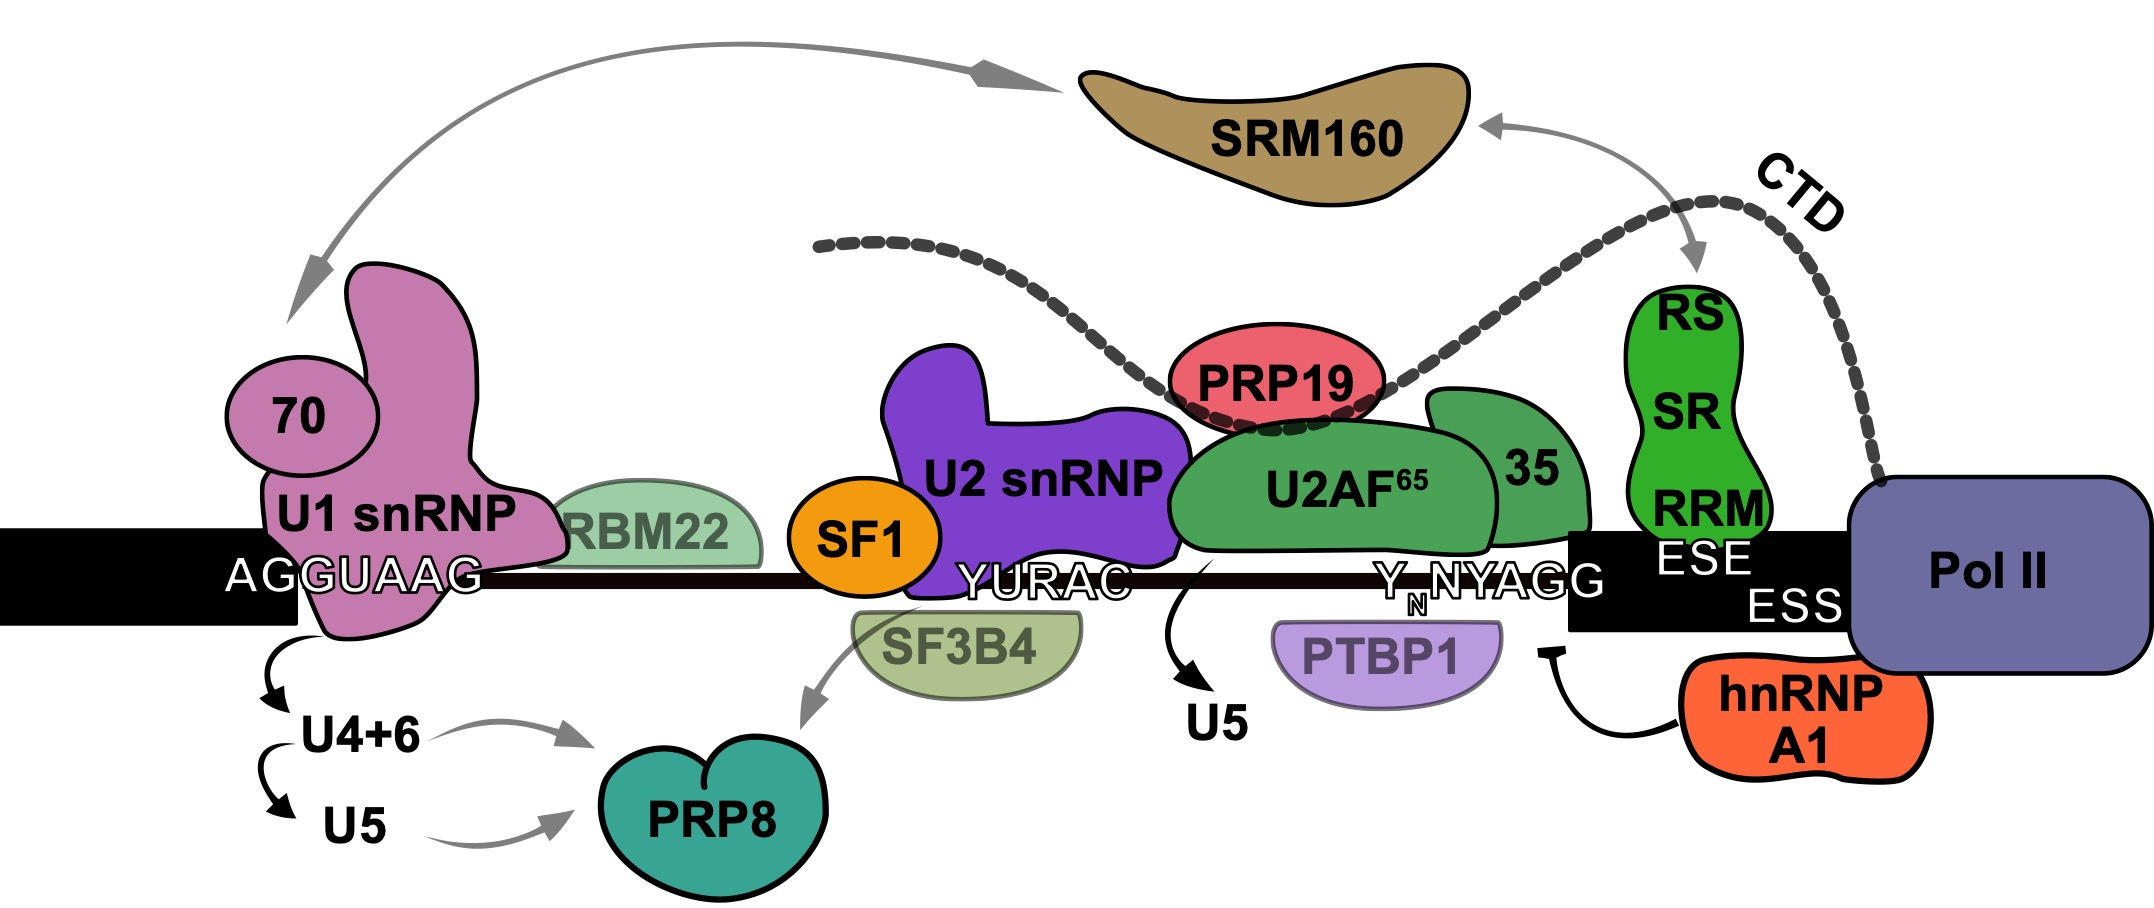
\includegraphics[width=0.95\linewidth]{slides/spliceosome.jpg}
  \caption{Some of the factors involved in splicing an intron (thin line) between two exons (black). U1 snRNP recognizes the $5'$ splice site (consensus AG$|$GUAAG); SF1, U2AF65/35 and U2 snRNP recognize the branch point (YURAC), polypyrimidine tract and $3'$ splice site (Y$_n$NYAG$|$G). An SR protein bound to an exonic splicing enhancer (ESE) and hnRNP A1 bound to an exonic splicing silencer (ESS) regulate the use of the downstream exon. The C-terminal domain (CTD) of Pol II helps recruit splicing factors co-transcriptionally. Drawn by the author.}
  \label{fig:spliceosome}
\end{figure}

This machinery is too complex to model from first principles, so splicing has been an early and productive application of machine learning in genomics: learn the mapping from sequence to splicing outcome from data. Two kinds of target have been used: the inclusion level of known alternative exons, and the location of splice sites anywhere in a pre-mRNA.

\subsection{Percent spliced in}

The \emph{percent spliced in} $\Psi\in[0,1]$ of an alternative exon in a sample is the fraction of the gene's transcripts that include it. It can be estimated from RNA-seq without solving the full isoform problem, by counting the reads that discriminate between inclusion and skipping (Figure~\ref{fig:psi}). Let $a$ be the number of reads that support inclusion, such as reads within the exon and junction reads joining it to a flanking exon, and $b$ the number that support exclusion, the junction reads joining the two flanking exons directly. After normalizing the counts for the number of positions at which each kind of read can arise (the inclusion isoform, for example, has two informative junctions and the skipping isoform one), the estimate is $\hat\Psi=a/(a+b)$.

\begin{figure}[!htbp]
  \centering
  \begin{tikzpicture}[every node/.style={font=\small}]
    \draw (0,0) -- (9,0);
    \fill (0.6,-0.2) rectangle (1.0,0.2);
    \draw[fill=white] (4.3,-0.2) rectangle (4.8,0.2);
    \fill (8.0,-0.2) rectangle (8.4,0.2);
    \node[above] at (4.55,0.25) {alternative exon};
    \node[left, align=right, font=\footnotesize] at (-0.1,0) {gene};
    % inclusion reads
    \foreach \y in {-0.6,-0.8,-1.0} {\draw[thick] (0.8,\y) -- (1.0,\y); \draw[densely dotted] (1.0,\y) -- (4.3,\y); \draw[thick] (4.3,\y) -- (4.45,\y);}
    \foreach \y in {-0.6,-0.8} {\draw[thick] (4.7,\y-0.6) -- (4.8,\y-0.6); \draw[densely dotted] (4.8,\y-0.6) -- (8.0,\y-0.6); \draw[thick] (8.0,\y-0.6) -- (8.2,\y-0.6);}
    \draw[thick] (4.35,-0.5) -- (4.75,-0.5);
    \draw[thick] (4.4,-0.7) -- (4.8,-0.7);
    \draw[decorate, decoration={brace, amplitude=4pt}] (9.1,-0.4) -- (9.1,-1.5) node[midway, right=5pt] {$a=7$ reads support inclusion};
    % exclusion reads
    \foreach \y in {-1.9,-2.1,-2.3} {\draw[thick] (0.75,\y) -- (1.0,\y); \draw[densely dotted] (1.0,\y) -- (8.0,\y); \draw[thick] (8.0,\y) -- (8.25,\y);}
    \draw[decorate, decoration={brace, amplitude=4pt}] (9.1,-1.8) -- (9.1,-2.4) node[midway, right=5pt] {$b=3$ reads support exclusion};
  \end{tikzpicture}
  \caption{Estimating the percent spliced in $\Psi$ of an alternative exon (white) from RNA-seq reads. Reads inside the exon and junction reads to it support inclusion; junction reads joining the flanking constitutive exons (black) support exclusion. After \citet{xiong2015}.}
  \label{fig:psi}
\end{figure}

The counts carry information about uncertainty as well. If each discriminating read independently supports inclusion with probability $\Psi$, then $a\mid\Psi\sim\Bin(a+b,\Psi)$, and with a uniform $\BetaD(1,1)$ prior the posterior is $\Psi\mid a,b\sim\BetaD(a+1,b+1)$, the $K=2$ case of the Dirichlet conjugacy of Section~\ref{sec:dirichlet}. Seven inclusion and three exclusion reads give the same point estimate as 70 and 30, but a much broader posterior (Figure~\ref{fig:psi_beta}). Models trained to predict $\Psi$ should account for this: an exon with few reads gives a noisy target.

\begin{figure}[!htbp]
  \centering
  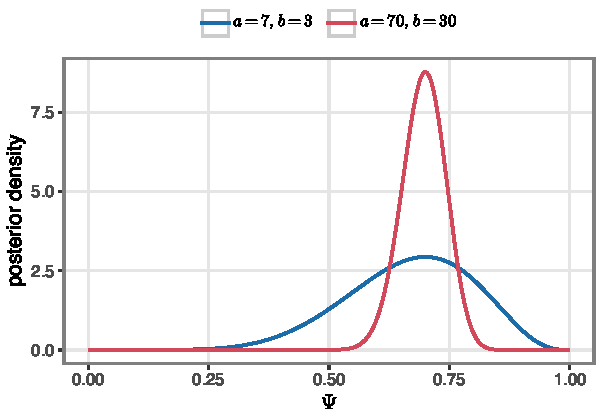
\includegraphics[width=0.55\linewidth]{psi_beta.pdf}
  \caption{Posterior distribution of $\Psi$ under a binomial model with a uniform prior, for $a=7$ inclusion and $b=3$ exclusion reads, and for ten times as many reads. Both have mode $0.7$; the posterior standard deviations are 0.13 and 0.045.}
  \label{fig:psi_beta}
\end{figure}

\subsection{The splicing code}

\citet{barash2010} and \citet{xiong2015} built models that predict $\Psi$ for an exon in a given tissue from its sequence and that of its neighbourhood, an approach they called the \emph{splicing code}. Training data came from RNA-seq of 16 human tissues, giving $\Psi$ for some ten thousand alternative exons in each. The model of \citet{xiong2015} is close to classical machine learning:
\begin{itemize}
  \item \emph{Targets.} The binomial model gives a distribution over $\Psi$ for each exon and tissue, with additional variance from bootstrap resampling of read positions. The loss is the KL divergence from this target distribution $P(\Psi)$ to the model's predicted distribution $Q(\Psi\mid\vx)$, where $\vx$ are the features, so noisy targets count for less.
  \item \emph{Features.} 1,393 hand-engineered features of the exon, its flanking introns and its neighbouring exons, including the presence of known splicing regulatory elements, splice site strength, \emph{translatability} (whether including or skipping the exon preserves the reading frame or introduces a premature stop codon), evolutionary conservation, and predicted nucleosome positioning.
  \item \emph{Model.} An ensemble of neural networks with two sigmoidal hidden layers, treated as Bayesian neural networks and fit by MCMC.
\end{itemize}
Some features are informative for an unusual reason. The spliceosome cannot check whether an exon preserves the reading frame, or whether its sequence is conserved in chimpanzees. These features are predictive because natural selection has shaped which exons are included: an exon whose inclusion would break the protein is unlikely to be included at high levels in a healthy tissue, and an exon whose sequence is conserved is more likely to be functional. A model using them partly learns the outcome of evolution rather than the mechanism of splicing, which matters when we use it to predict the effect of new mutations. Nucleosome features are relevant for a more mechanistic reason: transcription and splicing are coupled, and nucleosomes are enriched on exons.

The predictions correlate well with measured $\Psi$ across exons (Figure~\ref{fig:xiong}a), although with a sigmoidal bias. Predicting which exons are included is easier than predicting how inclusion of one exon changes between tissues, since differences between tissues are much smaller than differences between exons. A model that maps sequence to splicing can also be used in place of a mutagenesis experiment, as for the models of transcription factor binding in Chapters 2 and 4: run it on the reference and the variant sequence and take the difference $\Delta\Psi$ (Figure~\ref{fig:xiong}b). Applied to hundreds of thousands of genetic variants, predicted effects were largest within exons and in the first few tens of nucleotides of the flanking introns, near the splice sites, although some deeper intronic variants had large predicted effects too. Variants associated with disease had larger predicted effects than common variants, and this held for \emph{synonymous} exonic variants, which do not change the amino acid sequence, as well as for missense variants, which do. A synonymous variant can still change the protein by changing splicing.

\begin{figure}[!htbp]
  \centering
  \begin{subfigure}[b]{0.38\linewidth}
    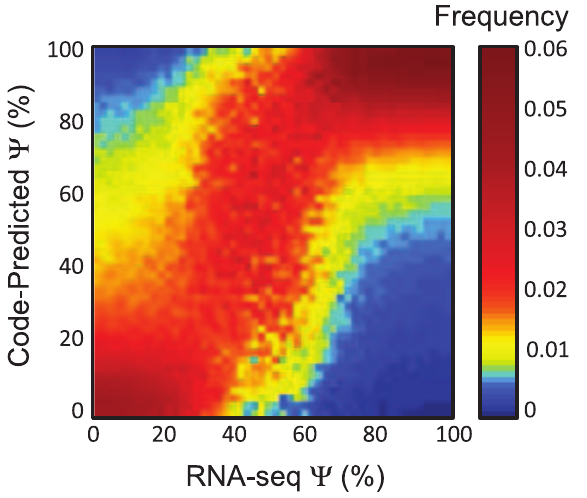
\includegraphics[width=\linewidth]{slides/xiong_psi_prediction.png}
    \caption{}
  \end{subfigure}\hfill
  \begin{subfigure}[b]{0.6\linewidth}
    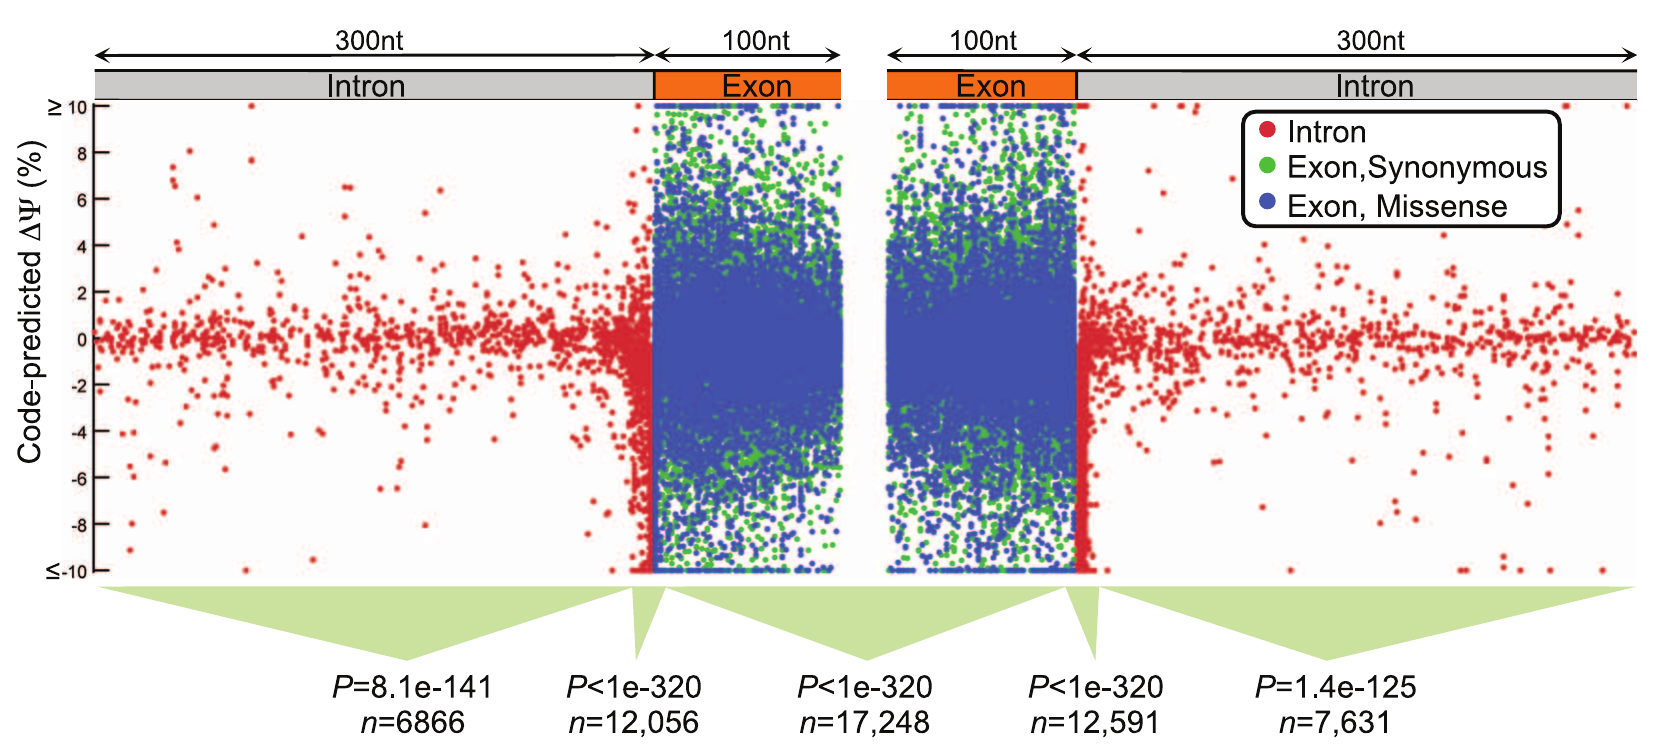
\includegraphics[width=\linewidth]{slides/xiong_delta_psi.png}
    \caption{}
  \end{subfigure}
  \caption{The splicing code. (a) Predicted against RNA-seq-measured $\Psi$ for 10,689 test exons in 16 tissues; for each bin of measured $\Psi$ (column) the colour shows the distribution of predictions. (b) Locations and predicted $\Delta\Psi$ of 81,608 disease-annotated intronic and exonic (synonymous or missense) variants, in the 300\,nt of intron and 100\,nt of exon on either side of each splice site; $|\Delta\Psi|$ is truncated at 10\%. Reproduced from \citet{xiong2015}.}
  \label{fig:xiong}
\end{figure}

\subsection{SpliceAI}

SpliceAI~\citep{jaganathan2019} takes a different approach. Rather than predicting the inclusion of known exons from engineered features, it predicts from sequence alone, at every position of a pre-mRNA, whether the position is a splice \emph{acceptor} (the end of an intron), a splice \emph{donor} (the start of an intron) or neither. This is a three-class classification problem at each position, trained with the cross-entropy loss of Chapter 1 against splice sites annotated in GENCODE transcripts, and tested on held-out chromosomes. The input is the one-hot encoded pre-mRNA sequence with up to 5,000\,nt of context on each side of each position. Long context matters because the spliceosome must choose among many candidate sites, and the right choice depends on the surrounding exons, introns and regulatory elements.

\paragraph{Architecture.} SpliceAI is a deep convolutional network built from two ingredients that we met in Chapter 3: residual connections and dilated convolutions (Figure~\ref{fig:resnet_dilated}).

A \emph{residual block}~\citep{he2016} computes $\vx+F(\vx)$ rather than $F(\vx)$, where $\vx$ is the block's input (the network input or the activations of an earlier layer) and $F$ is a small stack of layers. If the weights of $F$ are zero, the block is the identity, so a block can learn to do nothing, and with small initial weights each block starts close to the identity. The identity path also lets gradients pass directly to early layers, the same idea by which LSTM and GRU cells (Chapter 7) improve on a vanilla recurrent network. Residual connections made it possible to train much deeper networks for image recognition~\citep{he2016}. Since $\vx$ and $F(\vx)$ are added, they must have the same dimensions, so operations that change the resolution, such as max pooling, cannot be used inside a block. In SpliceAI each residual block is two repeats of batch normalization~\citep{ioffe2015}, a ReLU and a convolution (Figure~\ref{fig:spliceai_arch}).

A \emph{dilated convolution}~\citep{yu2016} with dilation $d$ applies its filter to input positions $d$ apart. For a one-dimensional input $f$ and a filter $k$ of width $W$, the output at position $t$ is
\begin{equation}
  (k *_d f)_t = \sum_{\tau} k_\tau\, f_{t-d\tau},
\end{equation}
where $\tau$ ranges over the $W$ filter positions; $d=1$ is ordinary convolution. Dilation is different from a stride, which moves the filter by more than one position between outputs and so reduces the resolution. A dilated convolution keeps one output per position but widens the stretch of input each output depends on. A width-$W$ convolution with dilation $d$ extends the receptive field by $(W-1)d$ positions, so increasing the dilation from layer to layer makes the receptive field grow much faster with depth than for ordinary convolutions.

\begin{figure}[!htbp]
  \centering
  \begin{tikzpicture}[>=Stealth, every node/.style={font=\small},
      box/.style={draw, minimum width=2.4cm, minimum height=0.5cm, fill=gray!8}]
    \node at (-1.6,4.4) {(a)};
    \node (x) at (0,4.4) {$\vx$};
    \node[box] (b1) at (0,3.5) {batch norm, ReLU};
    \node[box] (c1) at (0,2.8) {conv $(N,W,D)$};
    \node[box] (b2) at (0,2.1) {batch norm, ReLU};
    \node[box] (c2) at (0,1.4) {conv $(N,W,D)$};
    \node[circle, draw, inner sep=1pt] (plus) at (0,0.5) {$+$};
    \node (out) at (0,-0.3) {$\vx+F(\vx)$};
    \draw[->] (x) -- (b1); \draw[->] (b1) -- (c1); \draw[->] (c1) -- (b2); \draw[->] (b2) -- (c2); \draw[->] (c2) -- (plus); \draw[->] (plus) -- (out);
    \draw[->] (0,4.15) -- (1.8,4.15) -- (1.8,0.5) node[midway, right] {identity} -- (plus);
    \draw[decorate, decoration={brace, mirror, amplitude=4pt}] (-1.35,3.75) -- (-1.35,1.15) node[midway, left=5pt] {$F(\vx)$};
    % (b) dilated stack
    \begin{scope}[xshift=4.2cm, yshift=0.2cm]
      \node at (-0.5,4.2) {(b)};
      \foreach \lay/\lab in {0/input, 1/{$d=1$}, 2/{$d=2$}, 3/{$d=4$}} {
        \foreach \i in {0,...,16} \fill[gray!50] ({\i*0.45},{\lay*1.25}) circle (0.06);
        \node[right, font=\footnotesize] at (7.4,{\lay*1.25}) {\lab};
      }
      % connections for output unit at index 8
      \newcommand{\dconn}[3]{\draw[blue!70!black] ({(#1)*0.45},{(#3)*1.25}) -- ({(#2)*0.45},{(#3)*1.25-1.25});}
      \foreach \j in {-4,0,4} {\dconn{8}{8+\j}{3}}
      \foreach \cc in {4,8,12} {\foreach \j in {-2,0,2} {\dconn{\cc}{\cc+\j}{2}}}
      \foreach \cc in {2,4,6,8,10,12,14} {\foreach \j in {-1,0,1} {\dconn{\cc}{\cc+\j}{1}}}
      \foreach \i in {1,...,15} \fill[blue!70!black] ({\i*0.45},0) circle (0.07);
      \fill[blue!70!black] (8*0.45,3*1.25) circle (0.08);
      \draw[decorate, decoration={brace, mirror, amplitude=4pt}] (0.45,-0.25) -- (15*0.45,-0.25) node[midway, below=4pt, font=\footnotesize] {receptive field $1+2(1+2+4)=15$};
    \end{scope}
  \end{tikzpicture}
  \caption{(a) A residual block as used in SpliceAI: two repeats of batch normalization, ReLU and a convolution with $N$ channels, filter width $W$ and dilation $D$, added to the block input. (b) Three layers of width-3 convolutions with dilations 1, 2 and 4. The output unit (top) depends on 15 input positions; with ordinary convolutions it would depend on 7.}
  \label{fig:resnet_dilated}
\end{figure}

The largest model, SpliceAI-10k, first maps the one-hot input to 32 channels with a width-1 convolution, then applies 16 residual blocks in four groups of four, with filter width and dilation $(W,D)=(11,1)$, $(11,4)$, $(21,10)$ and $(41,25)$ (Figure~\ref{fig:spliceai_arch}). Every block has 32 channels, so the sequence length and channel number never change. In addition, the activations after each group pass through a width-1 convolution and are summed into the output, a skip connection over many blocks. A final width-1 convolution with three output channels and a softmax gives the acceptor, donor and neither probabilities at each position. Each residual block contains two convolutions, so the total receptive field is
\begin{align}
  1 + 2\times 4\times\left[(11-1)\cdot 1 + (11-1)\cdot 4 + (21-1)\cdot 10 + (41-1)\cdot 25\right]
  &= 1 + 8\times 1250 \nonumber\\
  &= 10{,}001
\end{align}
nucleotides, 5,000 on each side of the predicted position. The smaller models SpliceAI-80nt, -400nt and -2k use only the first one, two or three groups, and their receptive fields of 80, 400 and 2,000 nt (plus one) follow from the same calculation.

\begin{figure}[!htbp]
  \centering
  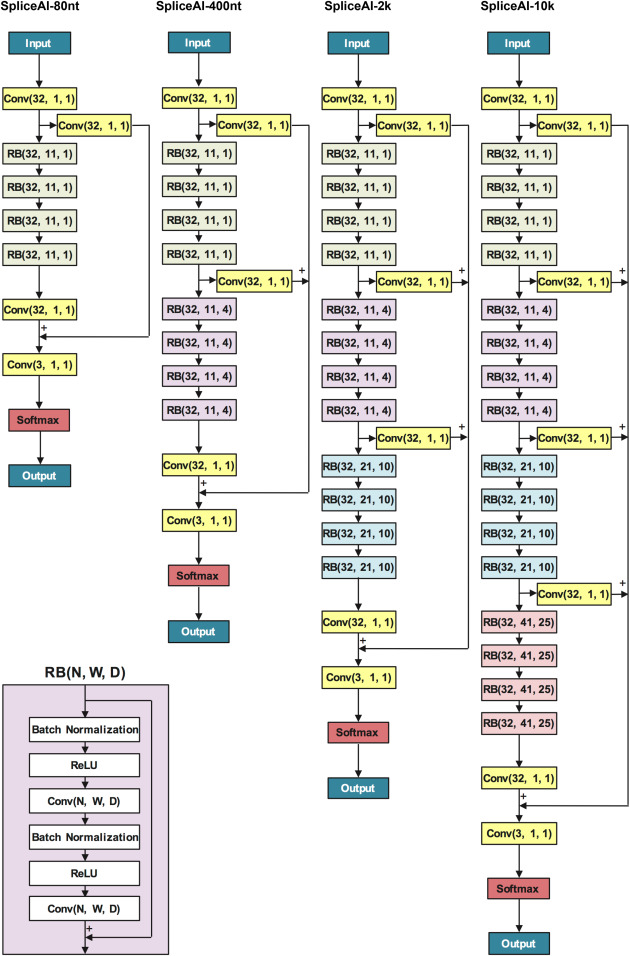
\includegraphics[width=0.48\linewidth]{slides/spliceai_architecture.png}
  \caption{SpliceAI architectures with increasing context. RB$(N,W,D)$ is a residual block with $N$ channels, filter width $W$ and dilation $D$ (inset); Conv$(N,W,D)$ is a convolution. Reproduced from \citet{jaganathan2019}.}
  \label{fig:spliceai_arch}
\end{figure}

\paragraph{Accuracy.} Splice sites are rare, a few per ten thousand positions, so accuracy is measured with metrics suited to class imbalance (Chapter 1). The \emph{top-$k$ accuracy} is computed by setting the threshold so that the number of positions called splice sites equals the actual number of splice sites $k$, and reporting the fraction of those $k$ calls that are correct; it is the precision at the point where precision equals recall. The second metric is the area under the precision-recall curve (PR-AUC). Accuracy increases with context (Table~\ref{tab:spliceai}). The earlier methods in the table use much shorter windows; MaxEntScan~\citep{yeo2004}, for example, scores 9\,nt around a donor and 23\,nt around an acceptor, so the comparison mainly shows how much the wider context helps.

\begin{table}[!htbp]
  \centering
  \caption{Splice site prediction on held-out chromosomes, from \citet{jaganathan2019}.}
  \label{tab:spliceai}
  \begin{tabular}{lcc}
    \toprule
    Model & Top-$k$ accuracy & PR-AUC \\
    \midrule
    SpliceAI-80nt & 0.57 & 0.60 \\
    SpliceAI-400nt & 0.90 & 0.95 \\
    SpliceAI-2k & 0.93 & 0.97 \\
    SpliceAI-10k & \textbf{0.95} & \textbf{0.98} \\
    \midrule
    GeneSplicer & 0.30 & 0.23 \\
    MaxEntScan & 0.22 & 0.15 \\
    NNSplice & 0.22 & 0.15 \\
    \bottomrule
  \end{tabular}
\end{table}

Figure~\ref{fig:spliceai_cftr}a shows predictions across the full pre-mRNA of \textit{CFTR}, the gene mutated in cystic fibrosis, about 189\,kb long with exons that are tiny compared with the introns. At the threshold that calls as many sites as there are true sites, SpliceAI-10k recovers almost all annotated acceptors and donors, while MaxEntScan's calls are scattered through the introns. In silico mutagenesis (Chapter 4) of the sequence around an acceptor (Figure~\ref{fig:spliceai_cftr}b) shows that the model relies on the AG and the polypyrimidine tract and on the GT at the downstream donor, and also on exonic motifs such as GAAGA, which resembles known ESEs.

\begin{figure}[!htbp]
  \centering
  \begin{subfigure}[b]{\linewidth}
    \centering
    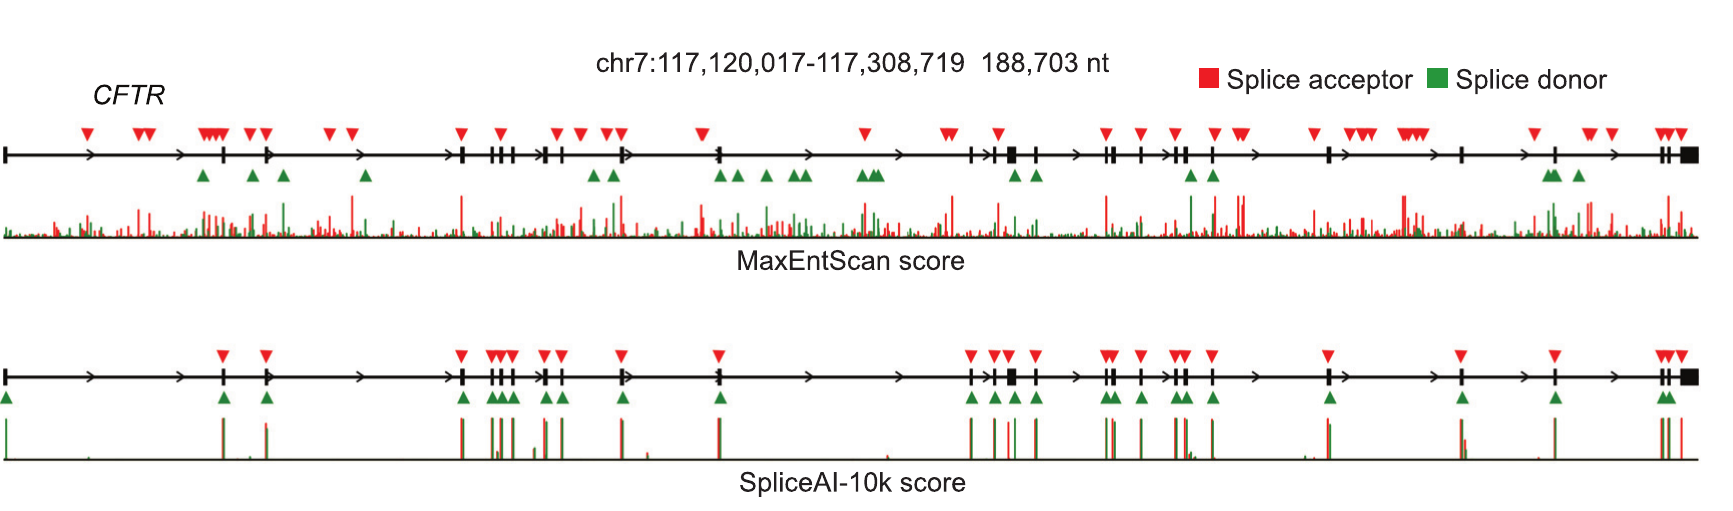
\includegraphics[width=0.85\linewidth]{slides/spliceai_cftr.png}
    \caption{}
  \end{subfigure}
  \begin{subfigure}[b]{\linewidth}
    \centering
    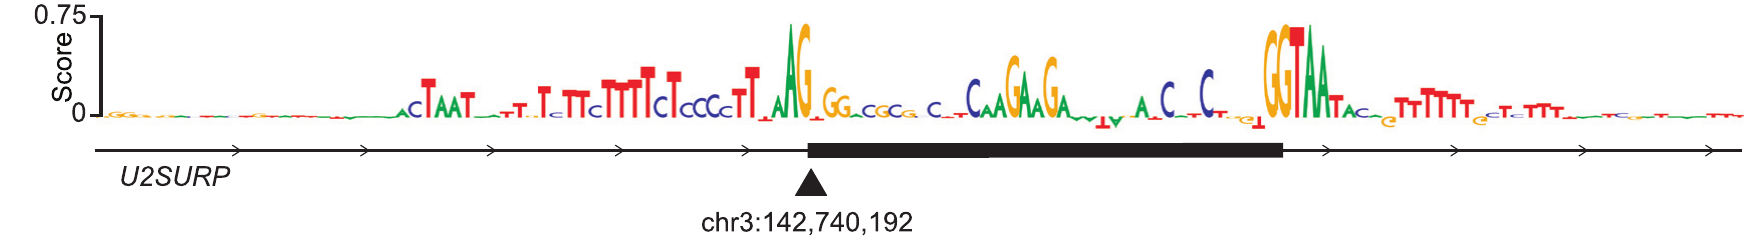
\includegraphics[width=0.85\linewidth]{slides/spliceai_saliency.png}
    \caption{}
  \end{subfigure}
  \caption{SpliceAI predictions. (a) The pre-mRNA of \textit{CFTR} scored by MaxEntScan (top) and SpliceAI-10k (bottom); triangles are predicted acceptors (red) and donors (green), and black boxes are the exons. (b) In silico mutagenesis around exon 9 of \textit{U2SURP}: the height of each nucleotide is the decrease in predicted acceptor strength at the black triangle when that nucleotide is mutated. Reproduced from \citet{jaganathan2019}.}
  \label{fig:spliceai_cftr}
\end{figure}

\paragraph{Variant effects.} To score a variant, SpliceAI is run on the reference and the alternative sequence, and the changes in predicted acceptor and donor probabilities at positions near the variant are summarized as four quantities: acceptor gain, acceptor loss, donor gain and donor loss. Their maximum, the $\Delta$ score between 0 and 1, is used to call variants splice-altering. Figure~\ref{fig:spliceai_pygb} shows an example confirmed by RNA-seq. A C$>$T variant in \textit{PYGB} creates a GT that is used as a new donor, shortening the exon by 35\,nt in the individual who carries it. Since 35 is not a multiple of 3, this shifts the reading frame of everything downstream.

\begin{figure}[!htbp]
  \centering
  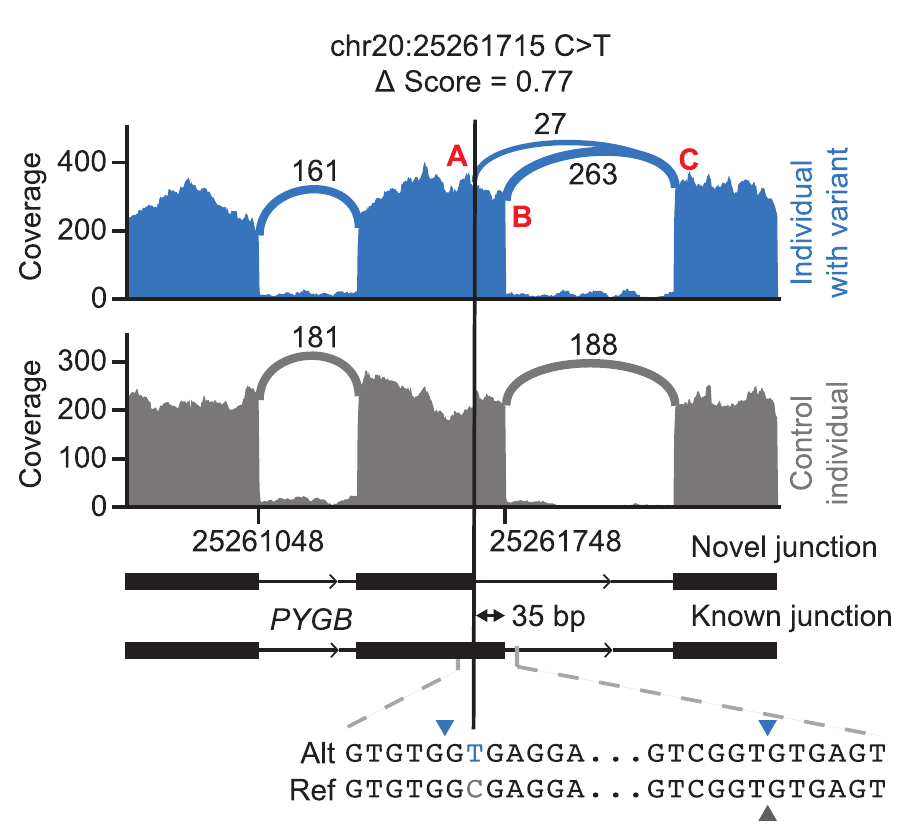
\includegraphics[width=0.6\linewidth]{slides/spliceai_pygb.png}
  \caption{A variant predicted by SpliceAI to create a donor ($\Delta$ score 0.77) in \textit{PYGB}. RNA-seq coverage and junction read counts (arcs) in an individual carrying the variant (blue) and a control individual (grey); the carrier uses a novel junction 35\,bp upstream of the known donor. Reproduced from \citet{jaganathan2019}.}
  \label{fig:spliceai_pygb}
\end{figure}

\paragraph{De novo mutations in neurodevelopmental disorders.} Autism spectrum disorder (ASD) and intellectual disability (ID) have a substantial contribution from \emph{de novo} mutations, mutations that arose in a parent's germ line and so are present in the child but in neither parent. Each person carries of the order of 70 de novo mutations, most of them harmless; the damaging ones in affected children are enriched in particular genes. \citet{jaganathan2019} scored de novo mutations from exome or genome sequencing of 4,293 individuals with ID from the Deciphering Developmental Disorders study~\citep{mcrae2017} and 3,953 individuals with ASD from the Simons Simplex Collection and the Autism Sequencing Consortium~\citep{turner2016,sanders2015}, and compared them with mutations in unaffected siblings. De novo mutations predicted to disrupt splicing were enriched in cases (Table~\ref{tab:denovo}), and counting them alongside protein-truncating mutations identified additional candidate genes. RNA-seq from affected individuals in the Simons Simplex Collection confirmed aberrant splicing for predicted variants, for example a de novo mutation in \textit{MED13}, a subunit of the Mediator complex that links transcription factors to Pol II.

\begin{table}[!htbp]
  \centering
  \caption{De novo mutations predicted by SpliceAI to disrupt splicing in intellectual disability (ID) and autism spectrum disorder (ASD) cohorts, compared with unaffected controls, as summarized from \citet{jaganathan2019}. The proportion is the estimated share of disease-causing de novo mutations that act through splicing.}
  \label{tab:denovo}
  \begin{tabular}{lcc}
    \toprule
    & ID ($n=4{,}293$) & ASD ($n=3{,}953$) \\
    \midrule
    Fold enrichment & 1.54 & 1.38 \\
    $p$-value & $<0.001$ & $<0.01$ \\
    Proportion of disease mutations & 7\% & 16\% \\
    New candidate genes & 5 & 2 \\
    \bottomrule
  \end{tabular}
\end{table}

Many of the genes implicated in ASD are expressed specifically in neurons and act at synapses, as one might expect, but many others are general regulators of transcription and chromatin, such as \textit{MED13}, expressed in every cell type. One explanation is that neurons, with their complex and long-lived gene expression programs, are especially sensitive to defects in such general machinery.

\subsection{Learning from random sequences}

All the models so far were trained on natural sequences. The human genome is large, but it contains a limited number of exons and introns, and the natural examples are confounded by evolution: as we saw, features such as conservation and translatability are predictive without being mechanisms. \citet{rosenberg2015} instead measured splicing for more than two million synthetic \emph{minigenes}. Each construct has fixed flanking exons and an intron of a few hundred nucleotides, much shorter than a typical human intron because of the cost of synthesizing long DNA, into which one or two random 25\,nt segments are inserted (Figure~\ref{fig:rosenberg}a). In the alternative $5'$ splice site library shown, two donors, SD$_1$ and SD$_2$, compete; the random sequence can strengthen or weaken them, create a new donor inside the random segment (SD$_\text{new}$) or activate a cryptic one (SD$_\text{crypt}$). A random barcode in the downstream exon identifies each construct after the library is transfected into cells and the spliced RNA is sequenced, so the usage of each splice site can be measured for every random sequence.

With this much unconfounded data, simple models work well. The \emph{hexamer additive linear} (HAL) model predicts the log-odds of using one splice site rather than another as a sum of weights, one per $k$-mer per random region, over the $k$-mers present: it is a linear model on $k$-mer counts. Figure~\ref{fig:rosenberg}b shows how accuracy depends on the amount of training data and on $k$. A $k$-mer model has $4^k$ features per region: 64 for $k=3$ and 16,384 for $k=7$. With little data the simplest model, using 3-mers, is most accurate, and it plateaus early because it cannot represent longer motifs. As the training set grows, models with longer $k$-mers overtake it, and with the full data set the 6-mer and 7-mer models are best. This illustrates the bias-variance trade-off of Chapter 1 directly: the best model complexity depends on how much data there is.

\begin{figure}[!htbp]
  \centering
  \begin{subfigure}[b]{\linewidth}
    \centering
    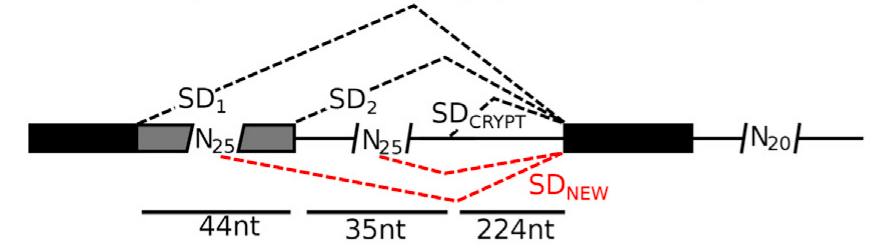
\includegraphics[width=0.6\linewidth]{slides/rosenberg_library.png}
    \caption{}
  \end{subfigure}
  \begin{subfigure}[b]{\linewidth}
    \centering
    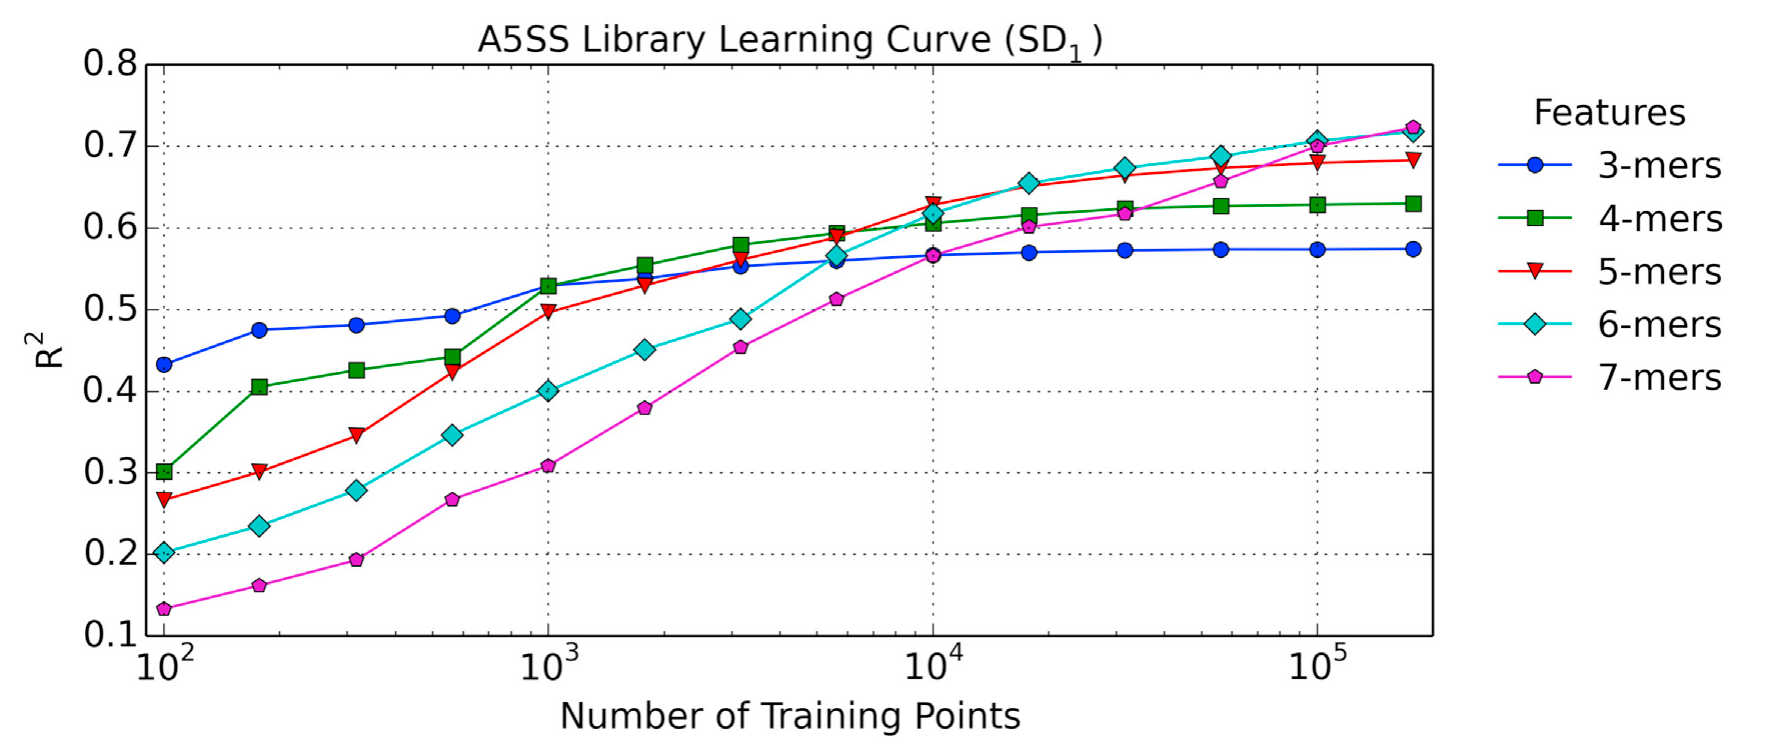
\includegraphics[width=0.8\linewidth]{slides/rosenberg_learning_curve.png}
    \caption{}
  \end{subfigure}
  \caption{Learning splicing from random sequences. (a) Design of the alternative $5'$ splice site library: fixed exons (black) and intron, random 25\,nt segments (N$_{25}$) near two competing donors (SD$_1$, SD$_2$), possible new and cryptic donors (red), and a random barcode (N$_{20}$). (b) Learning curves: held-out $R^2$ for predicting SD$_1$ usage with $k$-mer linear models, as a function of the number of training sequences. Reproduced from \citet{rosenberg2015}.}
  \label{fig:rosenberg}
\end{figure}

A model trained on synthetic sequences can be applied to natural ones. On a small set of variants in \textit{BRCA2}, \textit{CFTR} and \textit{SMN2} whose effects on splicing had been measured by RT-PCR, HAL's predicted $\Delta\Psi$ explained much more of the variance than SPANR, the splicing code model of \citet{xiong2015}, with $R^2=0.51$ against $0.17$ (Figure~\ref{fig:hal_spanr}). A linear model with large, unbiased training data beat a neural network trained on natural sequence, which suggests that the quality and diversity of training data, rather than model architecture, was the limiting factor. Neither model is accurate within any one gene, however.

\begin{figure}[!htbp]
  \centering
  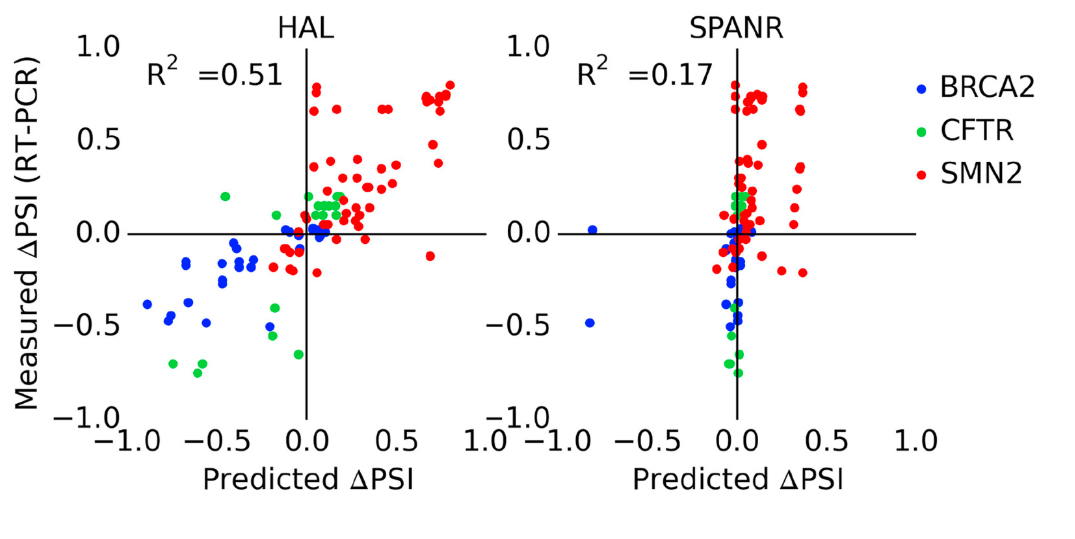
\includegraphics[width=0.6\linewidth]{slides/hal_vs_spanr.png}
  \caption{Predicted against measured (RT-PCR) changes in exon inclusion $\Delta\Psi$ for variants in three genes, for HAL, trained on random-sequence libraries, and SPANR~\citep{xiong2015}, trained on natural sequences. Reproduced from \citet{rosenberg2015}.}
  \label{fig:hal_spanr}
\end{figure}

%======================================================================
\section{Long-read RNA sequencing}
\label{sec:longreads}
%======================================================================

The short-read sequencing that made functional genomics a large field, mostly on Illumina instruments, now produces billions of reads per run, but each read is typically about 150\,nt, while human mRNAs are typically a few thousand nucleotides long. That mismatch is why isoform abundances have to be inferred with EM or variational inference. Long-read technologies aim to sequence whole RNA molecules, so that each read is an isoform (Figure~\ref{fig:long_reads}). Pacific Biosciences (PacBio) sequences circularized cDNA molecules repeatedly and combines the passes into an accurate consensus. Oxford Nanopore Technologies (ONT) pulls a DNA or RNA strand through a protein pore embedded in a membrane and infers the sequence from the changes in ionic current as the nucleotides pass through; it can sequence native RNA without reverse transcription. Nanopore reads have higher error rates than Illumina or PacBio reads, but throughput and accuracy have improved quickly, and large long-read RNA-seq data sets have appeared in the last few years. In practice many reads do not span the whole molecule, because of RNA degradation and incomplete reverse transcription; typical read lengths are around 1.5\,kb, enough to cover many but not all isoforms, so quantification still benefits from a model of which isoforms each read is compatible with.

\begin{figure}[!htbp]
  \centering
  \begin{tikzpicture}[every node/.style={font=\small}]
    \tikzset{ex/.style={minimum width=0.5cm, minimum height=0.25cm, inner sep=0pt}}
    \foreach \side/\xs/\title in {0/0/short reads, 1/6.6/long reads} {
      \begin{scope}[xshift=\xs cm]
        \node at (2.6,1.3) {\title};
        % three isoforms with exons at 0,1,2,3,4 (each 0.6 wide, spacing 1.1)
        \foreach \y/\col/\exs in {0.6/blue!60/{0,1,2,4}, 0.1/orange!70/{0,2,3,4}, -0.4/violet!60/{0,1,3,4}} {
          \draw[gray] (0,\y) -- (5.0,\y);
          \foreach \e in \exs \fill[\col] (\e*1.1,\y-0.12) rectangle (\e*1.1+0.6,\y+0.12);
        }
      \end{scope}
    }
    % short reads
    \foreach \x/\y in {0.1/-1.0, 0.9/-1.0, 2.3/-1.0, 3.5/-1.0, 4.5/-1.0, 0.4/-1.3, 1.3/-1.3, 2.9/-1.3, 4.0/-1.3, 0.0/-1.6, 1.9/-1.6, 3.3/-1.6, 4.6/-1.6}
      \draw[very thick, gray!70!black] (\x,\y) -- (\x+0.45,\y);
    \node[align=center, font=\footnotesize] at (2.6,-2.2) {which isoforms are present\\must be inferred};
    % long reads
    \begin{scope}[xshift=6.6cm]
      \foreach \y/\col/\exs in {-1.0/blue!60/{0,1,2,4}, -1.3/orange!70/{0,2,3,4}, -1.6/violet!60/{1,3,4}} {
        \foreach \e in \exs \draw[very thick, \col] (\e*1.1,\y) -- (\e*1.1+0.6,\y);
        \draw[densely dotted, \col] (0,\y) -- (5.0,\y);
      }
      \node[align=center, font=\footnotesize] at (2.6,-2.2) {each read spans most or all\\of one isoform};
    \end{scope}
  \end{tikzpicture}
  \caption{Short reads (left) cover a small part of an isoform and are often compatible with several; long reads (right) span most or all of a molecule, so its exon structure can be read off directly. The bottom long read is truncated at its $5'$ end, as many real reads are.}
  \label{fig:long_reads}
\end{figure}

Long-read data also enable a new kind of sequence model, one that predicts whole isoforms rather than individual splice sites or exons. \citet{saberi2024} cast this as language modelling. They extend the nucleotide alphabet so that each token records both the nucleotide and its role: uppercase A, C, G, U for exonic positions, lowercase for intronic positions, and four further letters for positions outside the gene. A gene sequence annotated with one isoform's structure then becomes a string, for example \texttt{XWZY\,AUGCAG\,guaagu\ldots{}uucag\,GUUCAA\,ZXWY} for an exon, an intron and a second exon flanked by sequence outside the gene (an invented example), and a model trained to predict the next token, a long-context state-space model of the kind mentioned in Chapter 7, learns jointly which sequences are transcribed and which are spliced out. Trained on long-read data, it can score or sample isoforms for a sequence. One limitation is that the model does not condition on cell type or condition, whereas splicing depends on both. Other approaches, including graph neural networks over the possible exon structures of a gene, are being developed.

%======================================================================
\section{Summary}
%======================================================================

\begin{itemize}
  \item Human genes consist of exons separated by much longer introns. The precursor RNA is capped, spliced and polyadenylated, mostly co-transcriptionally. Splicing removes introns in two steps defined by the GU donor, the branch point A and the AG acceptor.
  \item Alternative splicing, variation in which segments are removed, produces several isoforms per gene. It differs between tissues and development, as for 3R and 4R tau, and is disrupted in many diseases, including cancers driven by splicing factor mutations and neurodegeneration.
  \item Short RNA-seq reads are often compatible with several isoforms. A generative model with a Dirichlet prior on the read proportions $\vtheta$, a discrete latent origin for each read and a read likelihood $p_{nm}=y_{nm}/\tilde L_m$ underlies most quantification methods. EM alternates fractional assignment of reads to isoforms with re-estimation of $\vtheta$ from expected counts.
  \item Variational inference approximates an intractable posterior by the member of a tractable family closest in $\KL(q\|p)$, equivalently maximizing the ELBO. Under a mean-field factorization the CAVI update is $q_i\propto\exp\E_{-i}[\log p]$; for the isoform model it gives a Dirichlet posterior for $\vtheta$ and discrete posteriors for the read origins. CAVI needs conditionally conjugate models, underestimates posterior variance, and needs full passes over the data.
  \item Stochastic variational inference uses Monte Carlo estimates, made differentiable by the reparameterization trick, and minibatches, so that it applies to non-conjugate models and large data.
  \item Splicing can be predicted from sequence. Feature-based models predict exon inclusion $\Psi$; SpliceAI, a deep residual network of dilated convolutions with a 10\,kb receptive field, predicts splice sites at every position and scores the effects of variants, including de novo mutations in neurodevelopmental disorders. Models trained on millions of random sequences show the value of large, unconfounded training data.
  \item Long-read sequencing reads whole isoforms and supports models that predict complete isoform structures from sequence.
\end{itemize}

%======================================================================
\section*{Exercises}
%======================================================================

\begin{enumerate}
  \item Show that the mean of $\Dir(\va)$ is $a_k/a_\cdot$ and its mode is $(a_k-1)/(a_\cdot-K)$ when all $a_k>1$. (Hint: for the mean, use $\Gamma(x+1)=x\Gamma(x)$ and the normalizing constant of a Dirichlet with $a_k$ increased by one.)
  \item Show that the Dirichlet is conjugate to the discrete distribution: if $\vpi\sim\Dir(\va)$ and $t_1,\dots,t_N\mid\vpi\overset{\text{iid}}{\sim}\Disc(\vpi)$, then $\vpi\mid t_{1:N}\sim\Dir(\va+\mathbf{n})$, where $n_k=\sum_n\ind[t_n=k]$.
  \item A gene has two isoforms of effective lengths $\tilde L_1=1000$ and $\tilde L_2=500$. Isoform 2 is isoform 1 with a 500\,nt segment removed. Of $N=150$ reads, 50 fall in the segment unique to isoform 1 and 100 are compatible with both isoforms. Find the maximum likelihood $\vtheta$ by solving the EM fixed point, and convert it to molecule fractions $\tau_m$.
  \item Show that the log likelihood $\sum_n\log\sum_m\theta_m p_{nm}$ is concave in $\vtheta$, and give an example of reads and isoforms for which its maximum over the simplex is not unique.
  \item Derive the ELBO for the CAVI algorithm of Section~\ref{sec:vi} and verify that the terms in $\E[\log\theta_m]$ cancel when $\valpha'=\valpha+\sum_n\vphi_n$.
  \item For a bivariate Gaussian target with correlation $\rho$, show that the mean-field approximation minimizing $\KL(q\|p)$ has variances $\Sigma_{ii}(1-\rho^2)$, and find the mean-field approximation minimizing $\KL(p\|q)$ instead.
  \item Compute the receptive field of SpliceAI-2k from its architecture (Figure~\ref{fig:spliceai_arch}). How many residual blocks of width-11 ordinary (undilated) convolutions would be needed to reach the same receptive field?
  \item Implement EM and CAVI for a simulated three-isoform gene, and compare the CAVI posterior with samples from a Gibbs sampler that alternates $t_n\mid\vtheta$ and $\vtheta\mid t_{1:N}$.
\end{enumerate}

\bibliographystyle{abbrvnat}
\bibliography{../chapter10/chapter10}
\endgroup

% Generated wrapper: chapter 11 with its own figure path, macros and bibliography.
\graphicspath{{../chapter11/figures/}}
\makeatletter\def\input@path{{../chapter11/}}\makeatother
\begingroup
% Chapter 11: genome-wide association studies.
% Requires: amsmath, amssymb, bm, graphicx, booktabs, subcaption,
% tikz (arrows.meta, positioning, calc, decorations.pathreplacing, fit), natbib.
% Computed figures are produced by scripts/make_figures.py; figures/slides/ holds figures taken from the lecture slides.

\providecommand{\R}{\mathbb{R}}
\providecommand{\E}{\mathbb{E}}
\providecommand{\Normal}{\mathcal{N}}
\providecommand{\argmax}{\operatorname*{arg\,max}}
\providecommand{\argmin}{\operatorname*{arg\,min}}
\providecommand{\vy}{\mathbf{y}}
\providecommand{\vx}{\mathbf{x}}
\providecommand{\mX}{\mathbf{X}}
\providecommand{\mI}{\mathbf{I}}
\providecommand{\vb}{\boldsymbol{\beta}}
\providecommand{\veps}{\boldsymbol{\epsilon}}
\providecommand{\vp}{\mathbf{p}}
\providecommand{\vg}{\mathbf{g}}
\providecommand{\ind}{\mathbf{1}}
\providecommand{\vz}{\mathbf{z}}
\providecommand{\vzh}{\hat{\mathbf{z}}}
\providecommand{\ve}{\mathbf{e}}
\providecommand{\vu}{\mathbf{u}}
\providecommand{\vr}{\mathbf{r}}
\providecommand{\va}{\mathbf{a}}
\providecommand{\vc}{\mathbf{c}}
\providecommand{\vone}{\mathbf{1}}
\providecommand{\vgamma}{\boldsymbol{\gamma}}
\providecommand{\vtheta}{\boldsymbol{\theta}}
\providecommand{\vlambda}{\boldsymbol{\lambda}}
\providecommand{\mR}{\mathbf{R}}
\providecommand{\mK}{\mathbf{K}}
\providecommand{\mU}{\mathbf{U}}
\providecommand{\mS}{\mathbf{S}}
\providecommand{\mC}{\mathbf{C}}
\providecommand{\mA}{\mathbf{A}}
\providecommand{\mH}{\mathbf{H}}
\providecommand{\mZ}{\mathbf{Z}}
\providecommand{\Var}{\operatorname{Var}}
\providecommand{\Cov}{\operatorname{Cov}}
\providecommand{\logit}{\operatorname{logit}}

\chapter{Genome-wide association studies}
\label{ch:gwas}

So far this book has mostly modelled molecular measurements of cells: expression, chromatin accessibility, transcription factor binding, methylation. This chapter turns to the other main use of sequencing introduced in Chapter 1, reading the genomes of many individuals and relating the differences between them to traits and diseases. A genome-wide association study (GWAS) tests each of millions of genetic variants for association with a trait. Statistically, a GWAS is little more than millions of small linear or logistic regressions, but it has to deal with three complications that make it interesting from a machine learning point of view: the features (genotypes) are strongly correlated with their neighbours along the genome, the samples (people) are not independent because they share ancestry, and the effects are tiny and numerous. We first describe human genetic variation and how a GWAS is run, then the population genetics that creates correlation between variants, then the statistical tools built on top of GWAS results: linear mixed models for population structure, summary statistics, fine-mapping and LD score regression. We end with an example where the biology of a GWAS association was worked out in detail, the obesity association at the \textit{FTO} locus.

%======================================================================
\section{Human genetic variation}
\label{sec:variation}
%======================================================================

Humans are diploid: apart from the sex chromosomes, each person carries two copies of every chromosome, one inherited from each parent. The human genome is about $3\times10^9$ base pairs (bp) long and contains roughly 20{,}000--25{,}000 protein-coding genes. Two copies of the genome, whether the two copies within one person or copies from two different people, differ at roughly one position in every thousand. A typical genome differs from the reference genome at 4--5 million sites~\citep{kg2015}. Almost all of these differences are inherited; a few dozen per person (of the order of 50--100) are \emph{de novo} mutations that arose in a parent's egg or sperm.

A position where the population carries more than one nucleotide is \emph{polymorphic}. The alternative versions are called \emph{alleles}. Most polymorphic positions are \emph{bi-allelic}, with two alleles. Genetic variants are classified by size:
\begin{itemize}
  \item \emph{Single nucleotide polymorphisms} (SNPs) change one nucleotide. There are about 3 million \emph{common} SNPs, conventionally those whose rarer allele has frequency above 5\% in a population, and many more rare ones, down to \emph{private} variants seen in one family and \emph{de novo} variants seen in one person.
  \item \emph{Indels} are short insertions or deletions, up to about 50 bp.
  \item \emph{Structural variants} are larger insertions, deletions (\emph{copy number variants}), inversions and other rearrangements, up to millions of bp.
\end{itemize}
All of these are \emph{germline} variants, present in every cell and passed on to children. \emph{Somatic} mutations arise in a single cell during a person's lifetime, by chance or through exposures such as tobacco smoke or ultraviolet light, and are inherited only by that cell's descendants. They drive cancer but are not the subject of this chapter.

At a bi-allelic SNP we call the allele in the human reference genome the \emph{reference} allele and the other the \emph{alternative} allele. The rarer of the two in a population is the \emph{minor} allele, and its frequency is the \emph{minor allele frequency} (MAF), at most $0.5$. A person's \emph{genotype} at the SNP is the unordered pair of alleles they carry, for example AA, AC or CC. We usually ignore which allele came from which parent. (The exception is \emph{imprinting}, where only the copy from one parent is expressed.)

Most SNPs are rare. Under the simplest population genetic model, a population of constant size with no selection, the expected number of SNPs at which the alternative allele is carried by $i$ of $n$ sampled chromosomes is proportional to $1/i$. Rare variants therefore make up most SNPs (Figure~\ref{fig:sfs}, blue). Real human populations have grown rapidly in the last few thousand years, which adds still more rare variants. Rare variants contribute little to the differences between two people, however. A person is heterozygous at a SNP with allele frequency $f$ with probability $2f(1-f)$, so most of the sites at which one person carries two different alleles are common SNPs (Figure~\ref{fig:sfs}, orange).

\begin{figure}[!htbp]
  \centering
  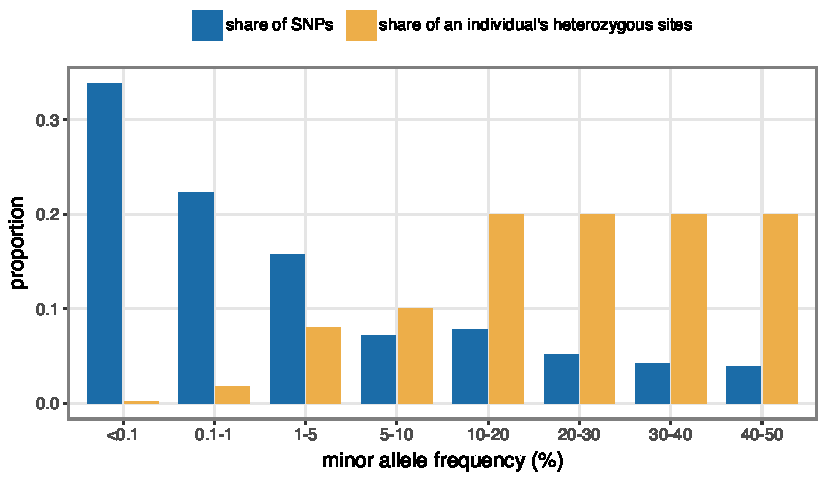
\includegraphics[width=0.75\linewidth]{sfs.pdf}
  \caption{Expected allele frequency distribution under the neutral constant-size model, for a sample of 20{,}000 chromosomes. Blue, the share of all SNPs in each minor allele frequency bin: most SNPs are rare. Orange, the share of the heterozygous sites of one individual: these are mostly common SNPs.}
  \label{fig:sfs}
\end{figure}

%======================================================================
\section{Why look for the genetic basis of disease?}
%======================================================================

There are three main motivations for mapping the genetic variants that affect disease risk.
\begin{enumerate}
  \item \emph{Understanding disease biology.} Complex diseases are often studied in animal models, for example mice engineered to carry human risk genes. These models reproduce some aspects of a human disease but not others. A mouse lives about two years, so a mouse model of a late-onset disease such as Alzheimer's disease has neurons that are two years old rather than seventy. Genetic associations come from human data, so they point at processes that matter in the human disease.
  \item \emph{Personalized prediction and treatment.} If we knew the variants that affect risk we could predict who is at higher risk and intervene earlier. This works well for some variants with large effects; for most common diseases, prediction from genotype remains modest.
  \item \emph{Identifying drug targets.} Retrospective analyses of drug development pipelines found that drug targets supported by human genetic evidence are about twice as likely to progress from clinical trials to approval~\citep{nelson2015,king2019} (Chapter 1). Given that bringing one drug to market costs of the order of a billion dollars, this is a strong argument for genetics.
\end{enumerate}

%======================================================================
\section{Mendelian and complex traits}
%======================================================================

\subsection{Mendelian genetics}

The first well-understood genetics was Gregor Mendel's work on pea plants~\citep{mendel1866}, decades before DNA was known to carry hereditary information. Consider one position in the genome with two alleles, A and T, and two parents that are both heterozygous, AT (Figure~\ref{fig:punnett}). Each gamete (pollen grain or egg cell in the plant, sperm or egg in a human) carries one copy of the genome, and so one of the parent's two alleles, chosen with probability $1/2$ each. Which gametes combine is also random, so an offspring is AA, AT or TT with probabilities $1/4$, $1/2$ and $1/4$.

In Mendel's flowers the A allele is \emph{dominant}: one copy is enough to make the flower purple, and only TT plants are white. The T allele is \emph{recessive}. A biochemical explanation could be that the T allele breaks an enzyme that makes purple pigment, and a single working copy of the enzyme makes enough pigment.

\begin{figure}[!htbp]
  \centering
  \begin{tikzpicture}[every node/.style={font=\small}, cell/.style={minimum width=1.6cm, minimum height=1.0cm, draw, align=center}]
    \node[cell, fill=yellow!25] at (1.6,1.0) {A};
    \node[cell, fill=blue!12] at (3.2,1.0) {T};
    \node[cell, fill=yellow!25] at (0,0) {A};
    \node[cell, fill=blue!12] at (0,-1.0) {T};
    \node[cell, fill=violet!35] at (1.6,0) {AA\\[-1pt]\footnotesize $1/4$};
    \node[cell, fill=violet!35] at (3.2,0) {AT\\[-1pt]\footnotesize $1/4$};
    \node[cell, fill=violet!35] at (1.6,-1.0) {TA\\[-1pt]\footnotesize $1/4$};
    \node[cell, fill=white] at (3.2,-1.0) {TT\\[-1pt]\footnotesize $1/4$};
    \node[above] at (2.4,1.55) {father's gamete (pollen)};
    \node[rotate=90, above] at (-0.85,-0.5) {mother's gamete};
    \node[right, align=left] at (4.3,0.0) {\tikz\fill[violet!35] (0,0) rectangle (0.3,0.2); purple flower (AA, AT)};
    \node[right, align=left] at (4.3,-0.6) {\tikz\draw (0,0) rectangle (0.3,0.2); white flower (TT)};
  \end{tikzpicture}
  \caption{A Punnett square for a cross between two heterozygous (AT) parents. Each gamete carries one allele, chosen at random, so each of the four combinations has probability $1/4$. With A dominant, three quarters of the offspring have the dominant (purple) phenotype.}
  \label{fig:punnett}
\end{figure}

Many human diseases follow this pattern. They are called \emph{Mendelian} diseases because a variant in a single gene is enough to cause them. Cystic fibrosis is a recessive disease caused by loss-of-function variants in \textit{CFTR}, which encodes a chloride channel~\citep{riordan1989}. It is the most common severe recessive disease in people of European ancestry, about 4\% of whom are heterozygous \emph{carriers}. Carriers are healthy, because one working copy suffices, but each child of two carriers has a $1/4$ chance of inheriting two broken copies, exactly as for the white flower. Marriage between relatives raises the probability that both parents carry the same rare recessive variant, inherited from a shared ancestor. Mendelian disease genes were mapped by following variants through families and are catalogued in Online Mendelian Inheritance in Man (OMIM).

\subsection{Complex traits}

Most common diseases, such as type 2 diabetes, schizophrenia and Alzheimer's disease, and quantitative traits such as height do not follow Mendelian patterns. They are called \emph{complex} traits. For these~\citep{manolio2009}:
\begin{itemize}
  \item no single variant is necessary or sufficient for disease;
  \item many genes and variants contribute, each with a small effect on risk, often raising it by a few percent;
  \item environment and chance also matter: diet and exercise for type 2 diabetes, for example;
  \item a single diagnosis can cover heterogeneous underlying mechanisms. Alzheimer's disease includes forms dominated by memory loss and forms dominated by language impairment, and neurodevelopmental conditions such as autism vary widely within a diagnosis;
  \item rare variants, \emph{de novo} mutations, interactions between variants (\emph{epistasis}) and parent-of-origin effects may contribute. Even the largest current studies are too small to test interactions between variants systematically, so most analyses assume that effects add up across the genome.
\end{itemize}
There are also indirect effects. Parents' genotypes affect their children's traits beyond the alleles the children inherit, for example through the environment the parents provide; this is sometimes called \emph{genetic nurture}~\citep{kong2018}.

Genome-wide association studies were designed for complex traits. The number of genome-wide significant associations has grown from a handful in 2006 to hundreds of thousands, catalogued in the GWAS Catalog~\citep{buniello2019}.

%======================================================================
\section{The genome-wide association study}
\label{sec:gwas_model}
%======================================================================

\subsection{Case-control association}

The simplest GWAS compares people who have a disease (\emph{cases}) with people who do not (\emph{controls}). Controls should be matched to cases on factors such as age: for a late-onset disease such as Alzheimer's, a young control may simply not have developed the disease yet. Each person is genotyped, traditionally with a genotyping array that measures a few hundred thousand chosen SNPs and increasingly by whole-genome sequencing. At each SNP we tabulate genotype counts in cases and controls and test whether genotype and disease status are independent (Figure~\ref{fig:casecontrol}).

\begin{figure}[!htbp]
  \centering
  \begin{tikzpicture}[every node/.style={font=\small}, >=Stealth]
    \node[anchor=west, inner sep=0] at (0,0.00) {\texttt{GGCATACG\textcolor{orange!80!black}{\textbf{A}}TATTAGCAA\textcolor{green!45!black}{\textbf{A}}TAAAC}};
    \node[anchor=west, inner sep=0] at (0,-0.42) {\texttt{GGCATACG\textcolor{orange!80!black}{\textbf{A}}TATTAGCAA\textcolor{green!45!black}{\textbf{A}}TAAAC}};
    \node[anchor=west, inner sep=0] at (0,-0.84) {\texttt{GGCATACG\textcolor{orange!80!black}{\textbf{A}}TATTAGCAA\textcolor{green!45!black}{\textbf{A}}TAAAC}};
    \node[anchor=west, inner sep=0] at (0,-1.26) {\texttt{GGCATACG\textcolor{orange!80!black}{\textbf{C}}TATTAGCAA\textcolor{green!45!black}{\textbf{G}}TAAAC}};
    \node[anchor=west, inner sep=0] at (0,-1.68) {\texttt{GGCATACG\textcolor{orange!80!black}{\textbf{C}}TATTAGCAA\textcolor{green!45!black}{\textbf{G}}TAAAC}};
    \node[anchor=west, inner sep=0] at (0,-2.10) {\texttt{GGCATACG\textcolor{orange!80!black}{\textbf{A}}TATTAGCAA\textcolor{green!45!black}{\textbf{A}}TAAAC}};
    \node[anchor=west, inner sep=0] at (0,-2.87) {\texttt{GGCATACG\textcolor{orange!80!black}{\textbf{A}}TATTAGCAA\textcolor{green!45!black}{\textbf{A}}TAAAC}};
    \node[anchor=west, inner sep=0] at (0,-3.29) {\texttt{GGCATACG\textcolor{orange!80!black}{\textbf{C}}TATTAGCAA\textcolor{green!45!black}{\textbf{G}}TAAAC}};
    \node[anchor=west, inner sep=0] at (0,-3.71) {\texttt{GGCATACG\textcolor{orange!80!black}{\textbf{C}}TATTAGCAA\textcolor{green!45!black}{\textbf{G}}TAAAC}};
    \node[anchor=west, inner sep=0] at (0,-4.13) {\texttt{GGCATACG\textcolor{orange!80!black}{\textbf{C}}TATTAGCAA\textcolor{green!45!black}{\textbf{G}}TAAAC}};
    \node[anchor=west, inner sep=0] at (0,-4.55) {\texttt{GGCATACG\textcolor{orange!80!black}{\textbf{C}}TATTAGCAA\textcolor{green!45!black}{\textbf{G}}TAAAC}};
    \node[anchor=west, inner sep=0] at (0,-4.97) {\texttt{GGCATACG\textcolor{orange!80!black}{\textbf{C}}TATTAGCAA\textcolor{green!45!black}{\textbf{G}}TAAAC}};
    \draw[decorate, decoration={brace, amplitude=4pt}] (-0.15,-2.3) -- (-0.15,0.2) node[midway, left=6pt] {controls};
    \draw[decorate, decoration={brace, amplitude=4pt}] (-0.15,-5.15) -- (-0.15,-2.65) node[midway, left=6pt] {cases};
    \foreach \k in {0,2,4} \draw[gray] (4.6,-\k*0.42+0.12) -- (4.75,-\k*0.42+0.12) -- (4.75,-\k*0.42-0.54) -- (4.6,-\k*0.42-0.54);
    \foreach \k in {6,8,10} \draw[gray] (4.6,-\k*0.42-0.23) -- (4.75,-\k*0.42-0.23) -- (4.75,-\k*0.42-0.89) -- (4.6,-\k*0.42-0.89);
    \node[anchor=west, align=left] at (4.9,-0.21) {one person};
    \node[anchor=north] at (1.55,-5.3) {SNP 1};
    \node[anchor=north] at (3.45,-5.3) {SNP 2};
    \node[anchor=west] at (6.6,-2.5) {%
      \begin{tabular}{lccc}
        \multicolumn{4}{c}{SNP 1 genotype counts}\\[2pt]
        \toprule
                 & AA & AC & CC \\
        \midrule
        controls & 1  & 2  & 0  \\
        cases    & 0  & 1  & 2  \\
        \bottomrule
      \end{tabular}};
  \end{tikzpicture}
  \caption{A cartoon case-control study with three controls and three cases, each carrying two copies of a short stretch of genome. Two positions are polymorphic (coloured). At SNP 1 (A or C) the genotype counts are tabulated in cases and controls and tested for association. Here SNP 2 (A or G) is perfectly correlated with SNP 1 in this sample, so it gives the same test result: correlation between nearby variants makes the causal variant hard to identify. Real studies involve tens or hundreds of thousands of people.}
  \label{fig:casecontrol}
\end{figure}

\subsection{Dosage and regression}

In practice each SNP is encoded as a \emph{dosage}, the number of copies of the alternative allele, $x\in\{0,1,2\}$: 0 for homozygous reference (AA, if A is the reference allele), 1 for heterozygous (AG) and 2 for homozygous alternative (GG). Some software counts the minor allele or the reference allele instead, which flips the sign of the effect, so the coding must be tracked when combining results.

Let $N$ be the number of individuals and $P$ the number of SNPs. Let $\mX\in\{0,1,2\}^{N\times P}$ be the genotype matrix, with entry $x_{is}$ the dosage of individual $i$ at SNP $s$ and column $\mX_{:s}\in\R^N$. Let $\vy\in\R^N$ be the phenotype and $\vc_i\in\R^Q$ a vector of $Q$ covariates for individual $i$, such as age, sex and the top genotype principal components (Section~\ref{sec:popstruct-11}). For each SNP $s$ in turn we fit the regression
\begin{equation}
  y_i = \beta_s x_{is} + \vgamma^\top\vc_i + \epsilon_i, \qquad \epsilon_i\overset{\text{iid}}{\sim}\Normal(0,\sigma^2),
  \label{eq:gwas_snp}
\end{equation}
where $\beta_s\in\R$ is the \emph{effect size} of SNP $s$ (the change in $y$ per copy of the alternative allele), $\vgamma\in\R^Q$ are the covariate coefficients and $\sigma^2$ the noise variance. For a binary trait we use logistic regression instead (Chapter 1), and $e^{\beta_s}$ is the \emph{odds ratio} per allele. The same per-SNP analysis is repeated for every one of the millions of SNPs. From a machine learning point of view it would be more natural to model all SNPs jointly. The per-SNP analysis is a pragmatic choice that scales easily, and, as we will see in Section~\ref{sec:sumstats}, the per-SNP results together with the correlations between SNPs retain most of the information in the data.

\paragraph{Estimate and test.} Consider one SNP with no covariates, and let $\tilde x_i = x_{is}-\bar x_s$ and $\tilde y_i=y_i-\bar y$ be centered genotype and phenotype. The least-squares estimate and its standard error are
\begin{equation}
  \hat\beta_s = \frac{\sum_i\tilde x_i\tilde y_i}{\sum_i\tilde x_i^2}, \qquad
  \operatorname{SE}(\hat\beta_s) = \frac{\hat\sigma}{\sqrt{\sum_i\tilde x_i^2}},
\end{equation}
where $\hat\sigma^2$ is the residual variance. If the two alleles a person carries are independent draws, each the alternative allele with probability $f_s$ (Hardy--Weinberg equilibrium), then $x_{is}$ is the sum of two independent Bernoulli($f_s$) variables, so $\Var(x_{is})=2f_s(1-f_s)$ and $\sum_i\tilde x_i^2\approx 2Nf_s(1-f_s)$. Rare variants therefore have large standard errors. To test the null hypothesis $\beta_s=0$ we use the Wald statistic
\begin{equation}
  \hat z_s = \frac{\hat\beta_s}{\operatorname{SE}(\hat\beta_s)},
\end{equation}
which is approximately $\Normal(0,1)$ under the null, so that $\chi^2_s=\hat z_s^2$ is approximately $\chi^2_1$ and the two-sided p-value is $2\Phi(-|\hat z_s|)$, with $\Phi$ the standard normal cumulative distribution function. Likelihood ratio tests give almost identical results at GWAS sample sizes. If $\mX_{:s}$ and $\vy$ are standardized to mean zero and variance one, $\hat\beta_s$ equals the sample correlation $r_s$ between genotype and phenotype, and $\hat z_s\approx\sqrt N r_s$ when $r_s$ is small.

\subsection{Multiple testing and the Manhattan plot}

Under the null hypothesis p-values are uniformly distributed, so at a threshold of 0.05 one in twenty null SNPs would appear significant. With millions of tests a much stricter threshold is needed. The Bonferroni correction divides the target error rate by the number of tests. SNPs are not independent tests, because nearby SNPs are correlated, and the effective number of independent common-variant tests in European-ancestry genomes was estimated to be about one million. The convention is therefore to call an association \emph{genome-wide significant} if $p<0.05/10^6=5\times10^{-8}$.

Results are displayed as a \emph{Manhattan plot} (Figure~\ref{fig:manhattan}): $-\log_{10}p$ for every SNP against its position, with chromosomes laid end to end. Associations appear as towers of points, because the SNPs correlated with an associated SNP are themselves associated. The towers are usually labelled with a nearby gene, but, as we will see, the nearest gene need not be the one through which the variant acts.

\begin{figure}[!htbp]
  \centering
  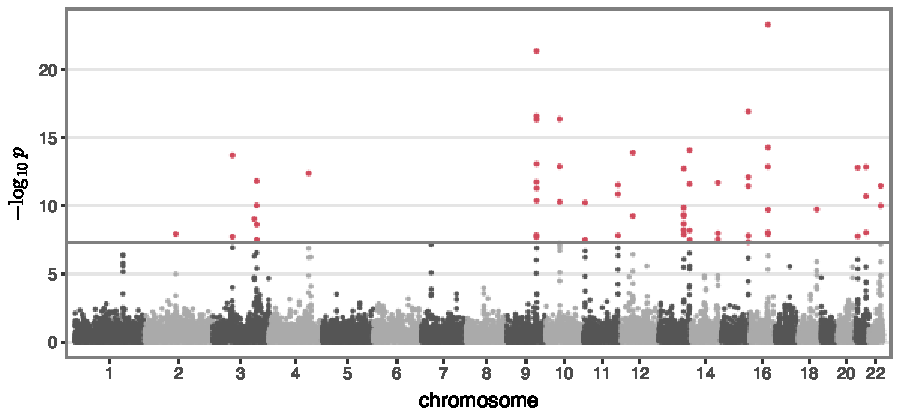
\includegraphics[width=0.9\linewidth]{manhattan.pdf}
  \caption{A Manhattan plot of a simulated GWAS of 23{,}000 SNPs. Each point is a SNP, placed by chromosome and position; the horizontal line marks genome-wide significance, $p=5\times10^{-8}$, and significant SNPs are red. Thirty causal variants were placed at random, with correlation between SNPs decaying with distance; each association appears as a tower of correlated SNPs. The z-scores were simulated from the summary statistic model of Section~\ref{sec:sumstats}.}
  \label{fig:manhattan}
\end{figure}

The early history of GWAS, in the mid-2000s, was marked by many associations that did not replicate in independent cohorts, because sample sizes of a few thousand were too small to detect realistic effects and statistical methods, particularly for population structure, were immature. With sample sizes now in the hundreds of thousands and the methods described in this chapter, GWAS associations replicate well~\citep{visscher2017}.

%======================================================================
\section{Recombination and linkage disequilibrium}
\label{sec:ld}
%======================================================================

\subsection{Inheritance and recombination}

Each of us inherits half of our genome from each parent, and therefore in expectation a quarter from each grandparent. This one fact determines how related any two relatives are. A parent and child share exactly half their genome in the sense that one of the child's two copies at every position came from that parent. Two full siblings also share half on average, but with some variance, because each received a random half from each parent. First cousins share one eighth on average.

The pieces we inherit are not whole chromosomes. During meiosis, the cell division that produces gametes, each pair of homologous chromosomes (the copy a parent received from their own mother and the copy from their own father) is duplicated into sister chromatids, and segments are exchanged between the homologs by \emph{crossing over}, or \emph{recombination} (Figure~\ref{fig:recomb}b). The chromosome passed on in a gamete is therefore a mosaic of the parent's two homologs: for example, a stretch from the paternal grandfather followed by a stretch from the paternal grandmother (Figure~\ref{fig:recomb}a). Each chromosome undergoes one to a few crossovers per meiosis. After many generations, a chromosome is a mosaic of small segments from many ancestors.

\begin{figure}[!htbp]
  \centering
  \newcommand{\chrom}[3]{% x, y, list of top/bottom/colour from the top (0) to the bottom (1)
    \foreach \t/\b/\c in {#3} {\fill[\c] (#1-0.12,#2-1.4*\t) rectangle (#1+0.12,#2-1.4*\b);}
    \draw[gray!60!black, rounded corners=1pt] (#1-0.12,#2) rectangle (#1+0.12,#2-1.4);}
  \begin{subfigure}[b]{0.58\linewidth}
    \centering
    \begin{tikzpicture}[every node/.style={font=\small}, person/.style={draw, very thick, gray, minimum width=1.0cm, minimum height=1.9cm}]
      % grandparents
      \node[person] (pgf) at (0,4.4) {}; \chrom{-0.2}{5.1}{0/1/blue!60}\chrom{0.2}{5.1}{0/1/red!60}
      \node[person, ellipse, minimum width=1.2cm] (pgm) at (1.8,4.4) {}; \chrom{1.6}{5.1}{0/1/green!60!black}\chrom{2.0}{5.1}{0/1/violet!60}
      \node[person] (mgf) at (4.0,4.4) {}; \chrom{3.8}{5.1}{0/1/cyan!70}\chrom{4.2}{5.1}{0/1/orange!80}
      \node[person, ellipse, minimum width=1.2cm] (mgm) at (5.8,4.4) {}; \chrom{5.6}{5.1}{0/1/brown!70}\chrom{6.0}{5.1}{0/1/lime!40}
      % parents
      \node[person] (fa) at (0.9,1.9) {}; \chrom{0.7}{2.6}{0/0.45/red!60,0.45/1/blue!60}\chrom{1.1}{2.6}{0/0.6/green!60!black,0.6/1/violet!60}
      \node[person, ellipse, minimum width=1.2cm] (mo) at (4.9,1.9) {}; \chrom{4.7}{2.6}{0/0.3/cyan!70,0.3/1/orange!80}\chrom{5.1}{2.6}{0/0.5/brown!70,0.5/1/lime!40}
      % child
      \node[person, ellipse, minimum width=1.2cm] (ch) at (2.9,-0.6) {}; \chrom{2.7}{0.1}{0/0.35/green!60!black,0.35/0.55/red!60,0.55/1/blue!60}\chrom{3.1}{0.1}{0/0.3/cyan!70,0.3/0.45/orange!80,0.45/0.6/brown!70,0.6/1/lime!40}
      \draw[gray, thick] (pgf.south) -- ++(0,-0.3) -| (pgm.south);
      \draw[gray, thick] (0.9,3.15) -- (fa.north);
      \draw[gray, thick] (mgf.south) -- ++(0,-0.3) -| (mgm.south);
      \draw[gray, thick] (4.9,3.15) -- (mo.north);
      \draw[gray, thick] (fa.south) -- ++(0,-0.3) -| (mo.south);
      \draw[gray, thick] (2.9,0.65) -- (ch.north);
      \node[left] at (-0.6,4.4) {grandparents};
      \node[left] at (0.3,1.9) {parents};
      \node[left] at (2.2,-0.6) {child};
    \end{tikzpicture}
    \caption{}
  \end{subfigure}\hfill
  \begin{subfigure}[b]{0.4\linewidth}
    \centering
    \begin{tikzpicture}[every node/.style={font=\small}]
      \chrom{0}{3}{0/1/red!60}\chrom{0.4}{3}{0/0.65/red!60,0.65/1/blue!50}
      \chrom{1.8}{3}{0/0.65/blue!50,0.65/1/red!60}\chrom{2.2}{3}{0/1/blue!50}
      \draw[decorate, decoration={brace, amplitude=3pt}] (-0.15,3.1) -- (0.55,3.1) node[midway, above=3pt, align=center, font=\footnotesize] {sister\\[-2pt]chromatids};
      \draw[decorate, decoration={brace, amplitude=3pt}] (1.65,3.1) -- (2.35,3.1) node[midway, above=3pt, align=center, font=\footnotesize] {sister\\[-2pt]chromatids};
      \draw[decorate, decoration={brace, amplitude=4pt}] (-0.2,4.05) -- (2.4,4.05) node[midway, above=4pt] {homologous chromosomes};
      \draw[decorate, decoration={brace, amplitude=3pt, mirror}] (0.3,1.5) -- (1.9,1.5) node[midway, below=3pt, align=center, font=\footnotesize] {exchanged by\\[-2pt]recombination};
    \end{tikzpicture}
    \caption{}
  \end{subfigure}
  \caption{(a) Inheritance through a pedigree (squares male, circles female). Each grandparent's two copies of one chromosome are given distinct colours. A parent passes on a mosaic of their two copies, so the child's paternal copy contains segments from both paternal grandparents. (b) Crossing over in meiosis. Each homologous chromosome (red, inherited from one parent; blue, from the other) is duplicated into two sister chromatids, and segments are exchanged between non-sister chromatids. Each resulting gamete receives one of the four chromatids.}
  \label{fig:recomb}
\end{figure}

Recombination is not uniform along the genome. In humans and many other mammals, most crossovers occur in \emph{recombination hotspots}, short regions of a few kilobases~\citep{myers2005}. Their positions are set largely by the zinc-finger protein PRDM9, which binds a specific DNA motif and marks nearby sites for recombination~\citep{baudat2010}. Dogs have lost a functional \textit{PRDM9} and lack such hotspots~\citep{axelsson2012}, and a woman with no functional PRDM9 was found to be healthy and fertile, with the crossovers in her children placed away from the usual hotspots~\citep{narasimhan2016}.

\subsection{Linkage disequilibrium}

Recombination is the reason that variants close together on a chromosome are correlated in a population. When a new mutation arises, it does so on one copy of the genome, alongside the particular alleles that copy carries at nearby SNPs. Over the following generations, recombination events between the mutation and a nearby SNP gradually break up this association, but if the two are close, a recombination between them is rare and the association persists for many generations. The non-random association of alleles at different loci is called \emph{linkage disequilibrium} (LD).

To quantify LD, consider two bi-allelic loci with alleles A/a and B/b, and let $f_A$ and $f_B$ be the frequencies of alleles A and B and $f_{AB}$ the frequency of haplotypes (single chromosome copies) carrying both A and B. If the loci were independent we would have $f_{AB}=f_Af_B$. The deviation
\begin{equation}
  D = f_{AB}-f_Af_B
\end{equation}
measures LD. Let $h_A\in\{0,1\}$ and $h_B\in\{0,1\}$ indicate whether a randomly chosen haplotype carries A and B. Then $\Cov(h_A,h_B)=\E[h_Ah_B]-\E[h_A]\E[h_B]=f_{AB}-f_Af_B=D$, and the squared correlation
\begin{equation}
  r^2 = \frac{D^2}{f_A(1-f_A)\,f_B(1-f_B)}
  \label{eq:r2}
\end{equation}
is the most widely used measure of LD. It lies between 0 (independence) and 1 (one allele perfectly predicts the other). The correlation between the dosages of two SNPs across individuals is approximately $r$ as well.

\paragraph{Decay of LD.} Let $c$ be the probability that a recombination occurs between the two loci in one meiosis, the \emph{recombination fraction}. Assume random mating in a large population and no selection. A haplotype in the next generation is non-recombinant with probability $1-c$, in which case it is a copy of a parental haplotype and carries A and B together with probability $f_{AB}$. With probability $c$ it is recombinant, its allele at the first locus comes from one parental haplotype and its allele at the second locus from the other, and in a randomly mating population these two haplotypes are independent, so it carries A and B with probability $f_Af_B$. Allele frequencies do not change, so the haplotype frequency and LD in the next generation are
\begin{align}
  f_{AB}' &= (1-c)f_{AB}+cf_Af_B,\\
  D' &= f_{AB}'-f_Af_B = (1-c)(f_{AB}-f_Af_B) = (1-c)D,
\end{align}
and after $t$ generations
\begin{equation}
  D_t = (1-c)^tD_0 .
\end{equation}
LD decays geometrically, at a rate set by the recombination fraction. For loci a few kilobases apart $c$ is of the order of $10^{-5}$ to $10^{-4}$, so LD can persist for thousands of generations. Recombination hotspots break LD sharply, so the genome is broken into \emph{LD blocks}, runs of SNPs with high mutual correlation separated by hotspots~\citep{gabriel2002}.

Random genetic drift in a finite population works in the opposite direction, creating LD by chance. The balance between the two depends on the effective population size and on the population's history. All modern humans descend from populations in Africa, and the ancestors of non-African populations left Africa around 60{,}000 years ago in a relatively small group that then expanded rapidly. This bottleneck means that non-African populations descend from fewer ancestral haplotypes and have had fewer generations of large population size, so LD extends further in non-African populations than in African populations~\citep{hapmap2005}, and African populations retain more genetic diversity than the rest of the world. Figure~\ref{fig:ld_heatmap} illustrates the effect in a simulation. A practical consequence is that association signals in African-ancestry cohorts are confined to fewer correlated SNPs, which helps to locate causal variants; most GWAS to date, however, have been in European-ancestry cohorts.

\begin{figure}[!htbp]
  \centering
  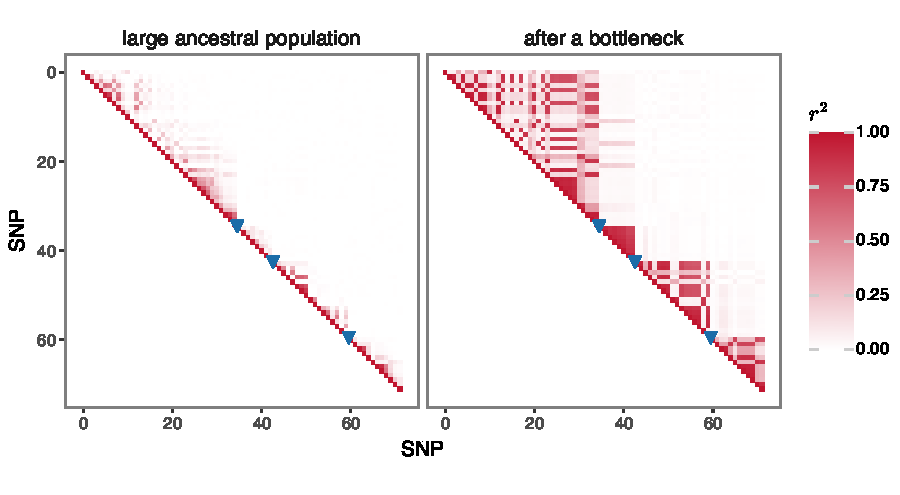
\includegraphics[width=0.9\linewidth]{ld_heatmap.pdf}
  \caption{Linkage disequilibrium ($r^2$ between pairs of SNPs, upper triangle) in two simulated populations of 1000 individuals that share recombination hotspots (triangles on the diagonal). Haplotypes were simulated as mosaics of ancestral founder haplotypes, switching founder rarely within blocks and often at hotspots. Left, a large population descended from 60 founder haplotypes with frequent historical recombination. Right, a population descended from 5 of the same founders with fewer generations of recombination, as after a bottleneck: LD is stronger and extends across blocks. SNPs with minor allele frequency above 5\% in both populations are shown in genomic order.}
  \label{fig:ld_heatmap}
\end{figure}

\subsection{LD and the causal variant}

LD is what makes a GWAS work with a few hundred thousand genotyped SNPs, since an untyped causal variant is detected through the typed SNPs correlated with it. It is also what makes it hard to tell which variant is causal. Figure~\ref{fig:fto_locus}A shows a \emph{LocusZoom} plot~\citep{pruim2010} of the strongest association with body mass index (BMI), in an intron of the gene \textit{FTO} on chromosome 16~\citep{frayling2007}. Each point is a SNP, placed by position and $-\log_{10}p$, and coloured by its $r^2$ with the most significant (lead) SNP. The blue line is the recombination rate, which peaks at two hotspots about 50 kb apart. Between them is an LD block of dozens of SNPs with p-values near $10^{-60}$, any of which could be causal. Panels B and C of the figure show how additional data can help, and we return to them in Section~\ref{sec:fto}.

\begin{figure}[!htbp]
  \centering
  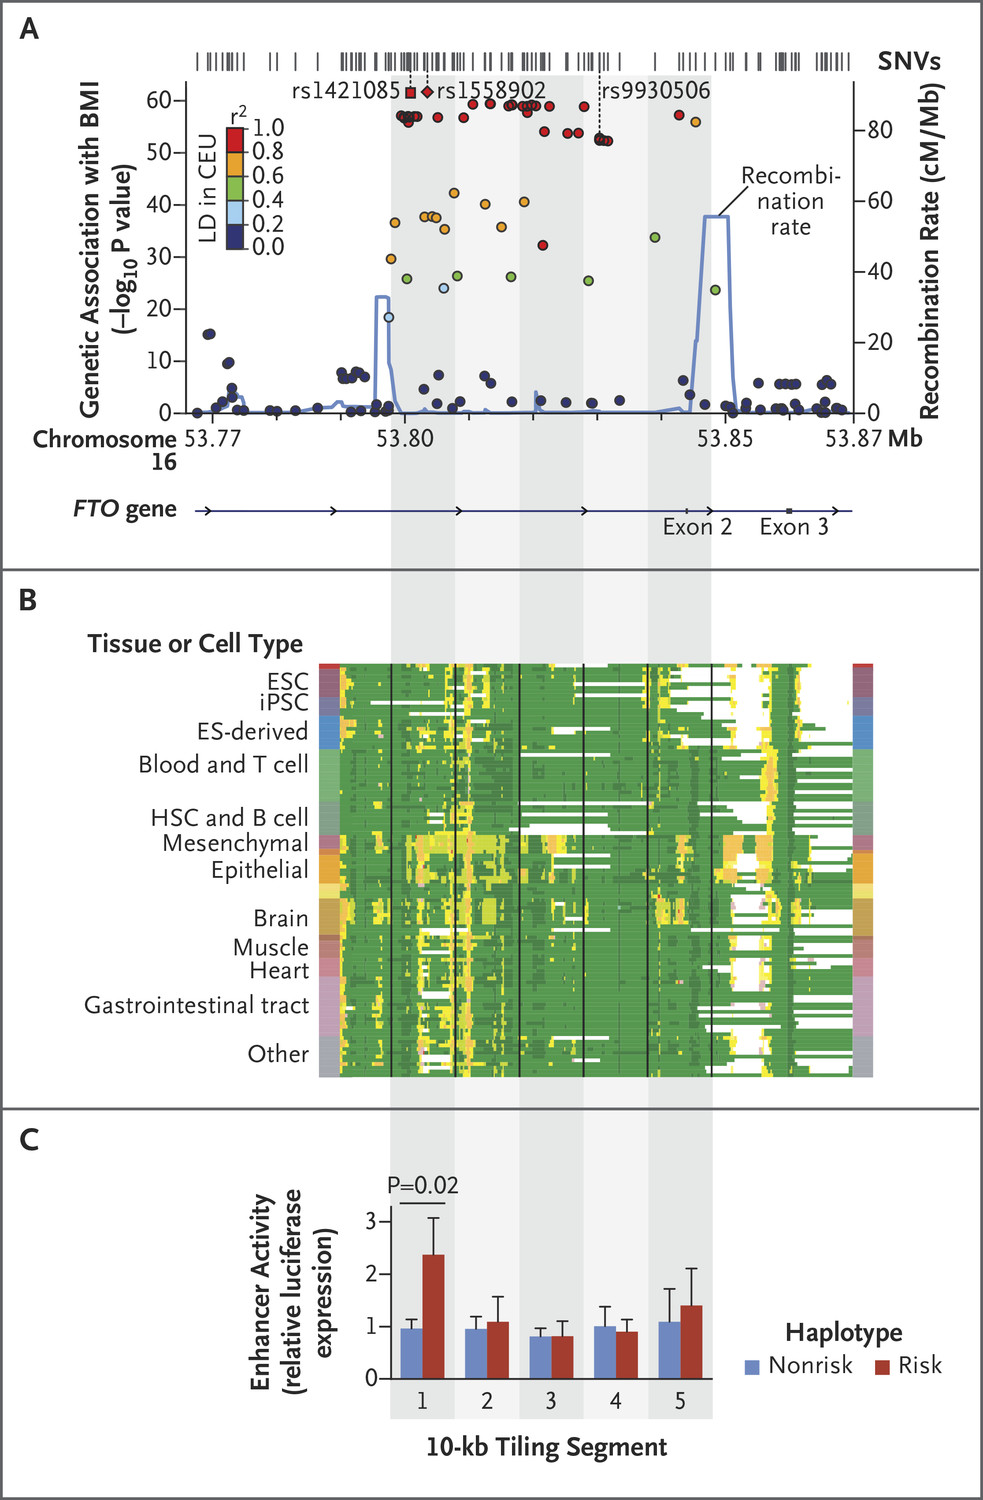
\includegraphics[width=0.62\linewidth]{slides/fto_locus.png}
  \caption{The \textit{FTO} obesity locus. (A) LocusZoom plot of association with BMI; colour shows LD ($r^2$) with the lead SNP in European-ancestry (CEU) reference data, and the blue line the recombination rate. (B) Chromatin states inferred by ChromHMM in 127 reference epigenomes grouped by tissue or cell type; yellow and orange states are enhancers. (C) Enhancer activity of five 10-kb segments of the locus, risk versus non-risk haplotype, in a luciferase reporter assay. Reproduced from \citet{claussnitzer2015}.}
  \label{fig:fto_locus}
\end{figure}

%======================================================================
\section{Genotyping arrays and imputation}
\label{sec:imputation}
%======================================================================

Whole-genome sequencing reads the genotype at every position, but most large GWAS cohorts were genotyped with arrays that measure 300{,}000--1{,}000{,}000 SNPs. LD makes it possible to predict, or \emph{impute}, the genotypes at the millions of SNPs that were not measured, using a \emph{reference panel} of sequenced individuals such as the 1000 Genomes Project~\citep{kg2015} (Figure~\ref{fig:imputation}).

\begin{figure}[!htbp]
  \centering
  \begin{tikzpicture}[every node/.style={font=\small}]
    \node (ref) at (0,0) {%
      \setlength{\tabcolsep}{3.5pt}\begin{tabular}{|cccccccccccc|}
        \hline
        0&0&1&1&1&0&0&1&0&1&1&0\\ \hline
        0&0&0&0&1&1&1&0&1&0&0&1\\ \hline
        1&1&1&1&0&0&0&1&0&0&0&0\\ \hline
        1&0&1&1&0&0&1&1&1&1&0&1\\ \hline
      \end{tabular}};
    \node (stu) at (0,-2.6) {%
      \setlength{\tabcolsep}{3.5pt}\begin{tabular}{cccccccccccc}
        1&\textcolor{red}{?}&\textcolor{red}{?}&2&\textcolor{red}{?}&0&\textcolor{red}{?}&\textcolor{red}{?}&1&\textcolor{red}{?}&\textcolor{red}{?}&1\\
        1&\textcolor{red}{?}&\textcolor{red}{?}&1&\textcolor{red}{?}&0&\textcolor{red}{?}&\textcolor{red}{?}&1&\textcolor{red}{?}&\textcolor{red}{?}&0\\
        0&\textcolor{red}{?}&\textcolor{red}{?}&1&\textcolor{red}{?}&1&\textcolor{red}{?}&\textcolor{red}{?}&2&\textcolor{red}{?}&\textcolor{red}{?}&1\\
        2&\textcolor{red}{?}&\textcolor{red}{?}&2&\textcolor{red}{?}&0&\textcolor{red}{?}&\textcolor{red}{?}&0&\textcolor{red}{?}&\textcolor{red}{?}&0\\
        1&\textcolor{red}{?}&\textcolor{red}{?}&\textcolor{red}{?}&\textcolor{red}{?}&1&\textcolor{red}{?}&\textcolor{red}{?}&1&\textcolor{red}{?}&\textcolor{red}{?}&2\\
      \end{tabular}};
    \draw[<->] ($(ref.south west)+(-0.3,-0.35)$) -- ($(ref.south east)+(0.3,-0.35)$) node[right] {genome};
    \draw[decorate, decoration={brace, amplitude=4pt}] ($(ref.north east)+(0.15,0)$) -- ($(ref.south east)+(0.15,0)$) node[midway, right=6pt, align=left] {reference haplotypes\\(sequenced panel)};
    \draw[decorate, decoration={brace, amplitude=4pt}] ($(stu.north east)+(0.15,0)$) -- ($(stu.south east)+(0.15,0)$) node[midway, right=6pt, align=left] {study genotypes\\(array; dosages 0/1/2)};
  \end{tikzpicture}
  \caption{The imputation problem. Reference haplotypes (top; 0 and 1 are the two alleles) are known at all SNPs. Study individuals (bottom) are genotyped at a subset of SNPs and their genotypes at the remaining SNPs (red question marks) are predicted from the reference panel using LD; missing calls at typed SNPs are filled in the same way. Adapted from a diagram on the IMPUTE2 website.}
  \label{fig:imputation}
\end{figure}

The simplest view of imputation is as a regression: for each untyped SNP, train a model in the reference panel that predicts its genotype from nearby typed SNPs, and apply it to the study individuals. The standard methods, such as IMPUTE2~\citep{howie2009}, instead use a hidden Markov model (Chapter 6) introduced by \citet{li2003}. Each haplotype of a study individual is modelled as a mosaic of the reference haplotypes, exactly as in the simulation of Figure~\ref{fig:ld_heatmap}. The hidden state at SNP $s$ is which reference haplotype is being copied. The transition probability of switching to another reference haplotype between adjacent SNPs increases with the genetic distance between them, mimicking historical recombination. The emission probability is close to 1 if the study allele matches the copied haplotype and small otherwise, allowing for mutation and genotyping error. The forward-backward algorithm gives the posterior probability of each genotype at each untyped SNP, and the imputed dosage is its posterior mean, $\E[x_{is}]=P(x_{is}=1)+2P(x_{is}=2)\in[0,2]$. These fractional dosages are used directly in the regression~\eqref{eq:gwas_snp}. Imputation accuracy is lower for rare variants, which are poorly tagged by typed SNPs, and when the reference panel does not match the ancestry of the study. Imputation matters for fine-mapping as well: a causal variant that is neither genotyped nor imputed can never be identified.

%======================================================================
\section{The genetic architecture of complex traits}
\label{sec:architecture}
%======================================================================

\subsection{Heritability and variance explained}

The \emph{heritability} $h^2$ of a trait is the fraction of its variance across individuals in a population that is explained by genetic differences. For a phenotype standardized to variance one, a single SNP with allele frequency $f_s$ and per-allele effect $\beta_s$ explains
\begin{equation}
  q_s^2 = \Var(\beta_sx_{is}) = \beta_s^2\Var(x_{is}) = 2f_s(1-f_s)\beta_s^2
  \label{eq:varexp}
\end{equation}
of the variance, using $\Var(x_{is})=2f_s(1-f_s)$ under Hardy--Weinberg equilibrium. The power to detect it depends on $Nq_s^2$. From Section~\ref{sec:gwas_model}, with standardized genotype and phenotype $\hat z_s\approx\sqrt N r_s$, and the sample correlation $r_s$ has mean approximately $\pm q_s$ and variance approximately $1/N$. Hence
\begin{equation}
  \E[\hat z_s^2]\approx 1+Nq_s^2,
\end{equation}
and $\hat z_s^2$ follows approximately a non-central $\chi^2_1$ distribution with non-centrality parameter (NCP) $Nq_s^2$. At $p<5\times10^{-8}$, that is $|\hat z_s|>5.45$, 80\% power requires an NCP of about 40. With $N=100{,}000$, this means $q_s^2\geq 4\times10^{-4}$: a SNP with $f_s=0.3$ needs $|\beta_s|\geq0.03$ phenotypic standard deviations per allele, while a SNP with $f_s=0.005$ needs $|\beta_s|\geq0.2$.

\subsection{Polygenicity}

One of the main findings of GWAS is that complex traits are highly \emph{polygenic}: they are affected by very many variants, each with a small effect. Before GWAS, many expected a typical disease to involve perhaps ten genes. The schizophrenia GWAS of the Psychiatric Genomics Consortium found 108 associated loci in 2014~\citep{ripke2014} and 287 in 2022 as the sample size grew~\citep{trubetskoy2022} (Figure~\ref{fig:scz-11}), and estimates of the total number of contributing variants are in the thousands. \citet{boyle2017} argued that gene regulatory networks are so densely connected that variants affecting the expression of almost any gene expressed in the relevant cell types will eventually have a small knock-on effect on the core genes of the trait. They called this the \emph{omnigenic} model.

\begin{figure}[!htbp]
  \centering
  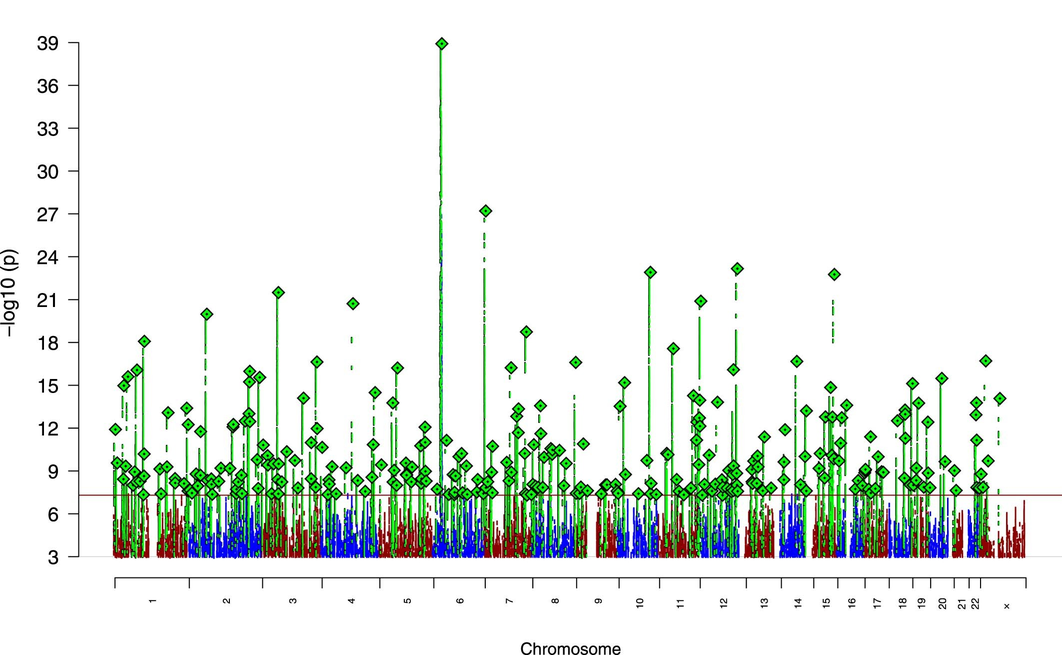
\includegraphics[width=0.7\linewidth]{slides/scz_manhattan.png}
  \caption{Manhattan plot of a schizophrenia GWAS, with 287 genome-wide significant loci (index SNPs as green diamonds above the red line, $p=5\times10^{-8}$). Reproduced from \citet{trubetskoy2022}.}
  \label{fig:scz-11}
\end{figure}

\subsection{Effect size and allele frequency}

Among associated variants there is an inverse relationship between effect size and minor allele frequency (Figure~\ref{fig:or_maf}). Common variants have odds ratios close to 1, while the few low-frequency variants with MAF below 1\% that reach significance have odds ratios of 2 or more.

\begin{figure}[!htbp]
  \centering
  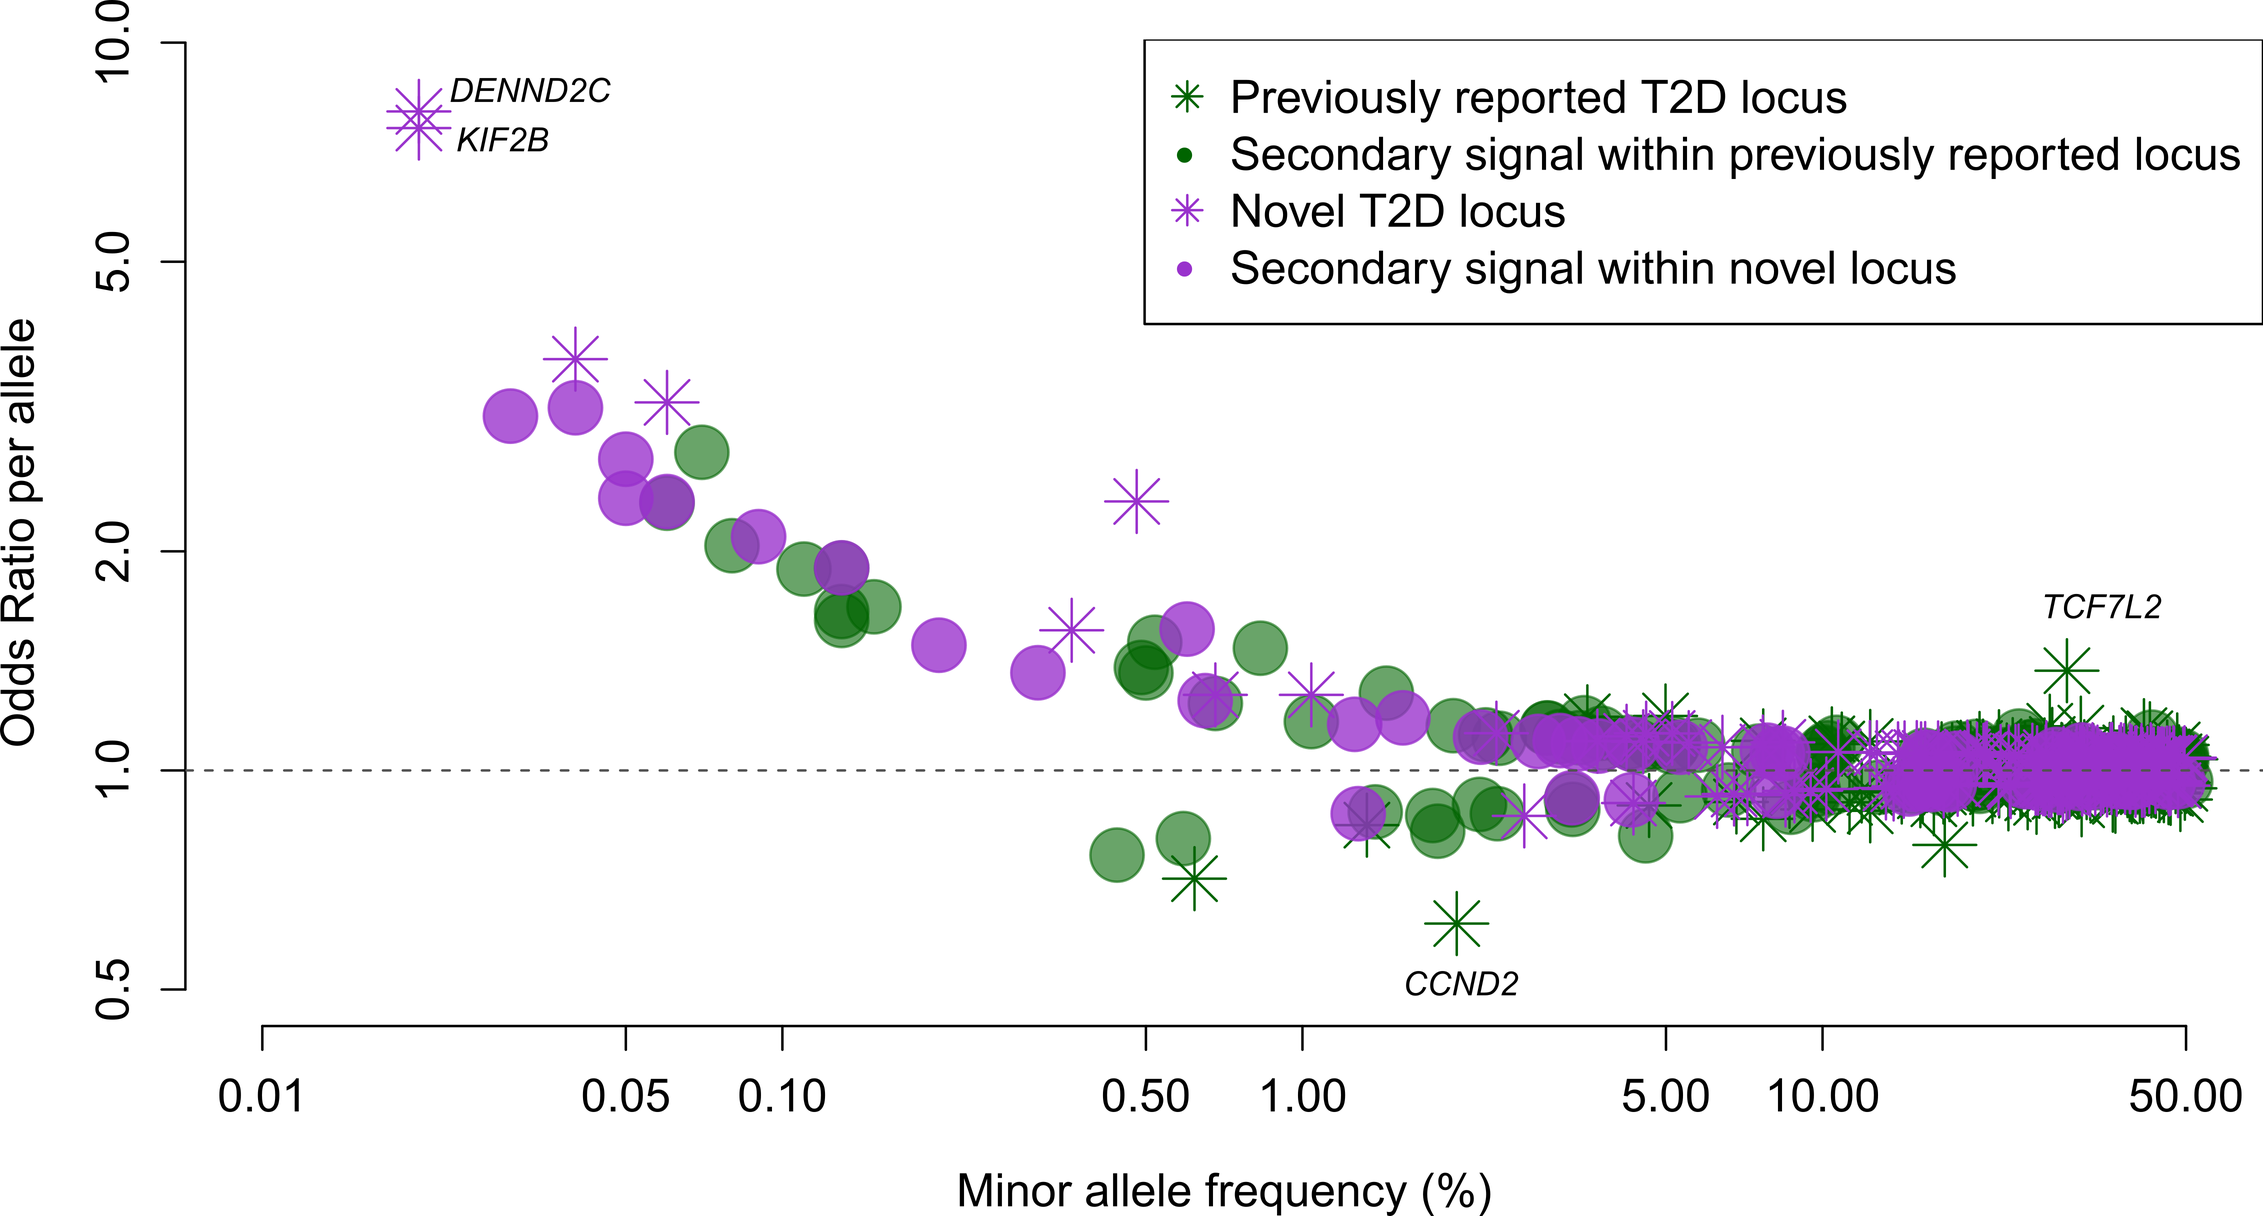
\includegraphics[width=0.7\linewidth]{slides/t2d_or_maf.png}
  \caption{Odds ratio per allele against minor allele frequency for 403 distinct association signals for type 2 diabetes, at previously reported and novel loci (stars, primary signals; circles, secondary signals). Reproduced from \citet{mahajan2018}.}
  \label{fig:or_maf}
\end{figure}

Two factors produce this pattern. The first is \emph{negative selection}. A variant that increases disease risk reduces, however slightly, its carriers' expected number of children, so natural selection acts to lower its frequency. Selection is more effective on variants with larger effects, which are therefore held at low frequency, while very rare variants are close to invisible to selection. A convenient model lets the variance of effect sizes depend on allele frequency,
\begin{equation}
  \Var(\beta_s\mid f_s)\propto\bigl[2f_s(1-f_s)\bigr]^{S},
\end{equation}
where $S\leq0$ measures the strength of the coupling: $S=0$ means effect sizes are independent of frequency, and $S=-1$ means each variant explains the same variance~\eqref{eq:varexp} on average whatever its frequency. Estimates for many human traits are negative~\citep{zeng2018}. Selection does not act on variants whose effects appear after reproductive age, which is one reason that strong risk alleles for late-onset diseases, such as the $\varepsilon4$ allele of \textit{APOE} for Alzheimer's disease, are common.

The second factor is \emph{power}. Since detection requires $2f_s(1-f_s)\beta_s^2$ to exceed a threshold, rare variants are detected only if their effects are large, whatever the underlying distribution of effects. Figure~\ref{fig:power_maf} separates the two factors in a simulation. Without selection, the discovered variants are almost all common. With $S=-1$, rare variants with large effects are frequent enough that many are discovered, and the discoveries show a strong inverse relationship. In both cases the discoveries lie just above the detection threshold.

\begin{figure}[!htbp]
  \centering
  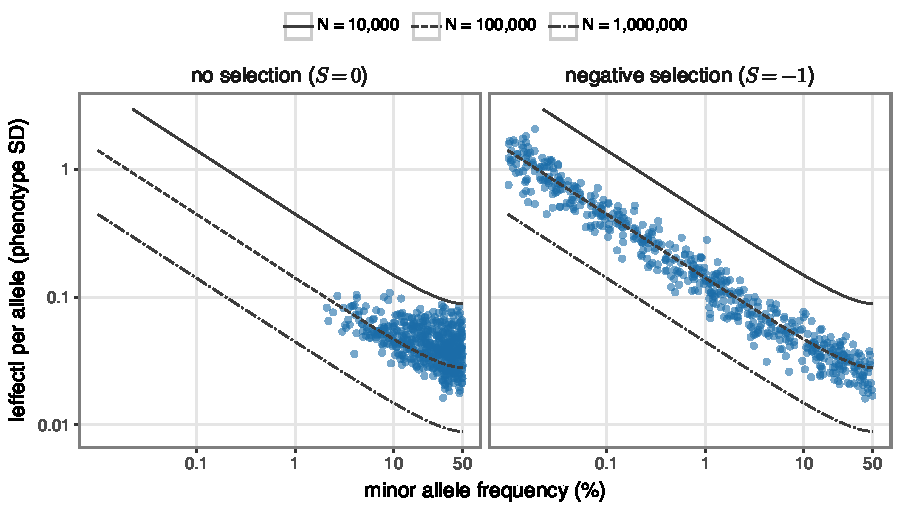
\includegraphics[width=0.9\linewidth]{power_maf.pdf}
  \caption{Lines, the per-allele effect (in phenotypic standard deviations) needed for 80\% power at $p<5\times10^{-8}$ for three sample sizes $N$, from~\eqref{eq:varexp}. Points, variants discovered in a simulated GWAS of $N=100{,}000$ individuals for a trait with heritability $0.5$ spread over 5000 causal variants, with minor allele frequencies drawn from the neutral spectrum and effect variance proportional to $[2f(1-f)]^S$. Left, no coupling between effect size and frequency ($S=0$): 524 variants are discovered, none with MAF below 1\%. Right, negative selection ($S=-1$): 545 discoveries, 267 with MAF below 1\%.}
  \label{fig:power_maf}
\end{figure}

%======================================================================
\section{Population structure and relatedness}
\label{sec:popstruct-11}
%======================================================================

\subsection{Confounding by ancestry}

The regression~\eqref{eq:gwas_snp} assumes independent noise. Two features of real samples violate this. The first is \emph{population structure} or \emph{stratification}: the sample contains people of different ancestry, allele frequencies differ by ancestry, and so does the phenotype, for genetic or environmental reasons. Then every SNP whose frequency differs between ancestry groups is associated with the phenotype, causal or not. A classic example comes from the Pima and Tohono O'odham communities of Arizona, where a haplotype of the immunoglobulin gene region \textit{Gm} was associated with lower risk of type 2 diabetes. The haplotype is common in Europeans and marked European admixture, which was itself associated with lower diabetes risk; within groups with the same degree of admixture the association disappeared~\citep{knowler1988}.

The second is \emph{relatedness}. Relatives share more of their genomes than unrelated people, and, for a heritable trait, more of their genetic predisposition. Unknown relatives in a sample (\emph{cryptic relatedness}) make the noise in~\eqref{eq:gwas_snp} correlated, so test statistics are inflated even at SNPs with no effect. Related individuals can be removed, but in large biobanks that discards many samples.

A simple diagnostic is the \emph{genomic inflation factor}~\citep{devlin1999}
\begin{equation}
  \lambda_{GC} = \frac{\operatorname{median}_s\,\hat z_s^2}{0.455},
\end{equation}
where 0.455 is the median of the $\chi^2_1$ distribution, so $\lambda_{GC}\approx1$ if most SNPs are null and the tests are calibrated. Dividing all $\chi^2$ statistics by $\lambda_{GC}$ (\emph{genomic control}) is a crude correction. As we will see in Section~\ref{sec:ldsc}, polygenicity alone also gives $\lambda_{GC}>1$ in large studies, so inflation is not by itself evidence of confounding.

\subsection{Genotype principal components}

Chapter 8 showed that the top principal components (PCs) of the standardized genotype matrix capture ancestry; for Europeans the first two reproduce a map of Europe. Including the top PCs as covariates $\vc_i$ in~\eqref{eq:gwas_snp} removes the part of genotype and phenotype explained by broad ancestry gradients~\citep{price2006}. By the Frisch--Waugh theorem, this is equivalent to regressing both $\mX_{:s}$ and $\vy$ on the PCs and testing the residuals. PCs work well for continuous ancestry gradients but do not capture fine-scale structure or family relationships.

\subsection{Linear mixed models}

A linear mixed model (LMM) accounts for both structure and relatedness. Let $s$ index the SNP being tested, $\mC\in\R^{N\times Q}$ the covariate matrix (including a column of ones) with coefficients $\vgamma\in\R^Q$, and $\beta_s\in\R$ the effect of SNP $s$. The model is
\begin{equation}
  \underbrace{\vy}_{N\times1} = \underbrace{\mX_{:s}}_{N\times1}\underbrace{\beta_s}_{1\times1} + \mC\vgamma + \underbrace{\vu}_{N\times1} + \underbrace{\veps}_{N\times1},\qquad
  \vu\sim\Normal(\mathbf{0},\sigma_g^2\mK),\qquad \veps\sim\Normal(\mathbf{0},\sigma_e^2\mI),
  \label{eq:lmm}
\end{equation}
where $\vu$ is a \emph{random effect} with covariance proportional to a relatedness matrix $\mK\in\R^{N\times N}$, $\sigma_g^2$ is the genetic variance component and $\sigma_e^2$ the noise variance. The usual choice is the \emph{realized relatedness matrix}
\begin{equation}
  \mK = \frac1P\mZ\mZ^\top,
\end{equation}
where $\mZ\in\R^{N\times P}$ is the genotype matrix with each column standardized to mean zero and variance one. Entry $K_{ii'}=\frac1P\sum_jZ_{ij}Z_{i'j}$ is the average over SNPs of the product of the two individuals' standardized genotypes. It is close to 1 for $i=i'$ and for identical twins, about $1/2$ for parents and children or siblings, $1/8$ for first cousins and near 0 for unrelated people. It is called ``realized'' because it estimates the relatedness actually realized in the genotypes rather than the relatedness expected from a pedigree. People of similar ancestry also have larger $K_{ii'}$, because they tend to share the alleles that are common in their ancestry group, so $\mK$ captures population structure too.

There is a useful interpretation of the random effect. Suppose all $P$ SNPs affect the trait, $\vu=\mZ\boldsymbol{\alpha}$, with independent effects $\alpha_j\sim\Normal(0,\sigma_g^2/P)$. Then $\Cov(\vu)=\mZ\,(\sigma_g^2/P)\mI\,\mZ^\top=\sigma_g^2\mK$. The LMM is therefore a joint regression on all SNPs with a Gaussian prior on their effects, which is ridge regression (Chapter 1), combined with a fixed effect for the SNP under test. Under this model $\sigma_g^2/(\sigma_g^2+\sigma_e^2)$ is the heritability explained by the SNPs~\citep{yang2010}. The background polygenic effect $\vu$ absorbs the phenotypic similarity of relatives and of people with shared ancestry, so it is not attributed to the test SNP.

\paragraph{Likelihood.} Integrating out $\vu$ and $\veps$, which are independent and Gaussian,
\begin{equation}
  \vy\sim\Normal\bigl(\mA\vtheta,\ \sigma_g^2\mK+\sigma_e^2\mI\bigr) = \Normal\bigl(\mA\vtheta,\ \sigma_g^2\mH\bigr),\qquad \mH=\mK+\delta\mI,
\end{equation}
where $\mA=[\mC,\mX_{:s}]\in\R^{N\times(Q+1)}$ collects the fixed-effect covariates, $\vtheta=(\vgamma^\top,\beta_s)^\top\in\R^{Q+1}$, and $\delta=\sigma_e^2/\sigma_g^2$. The log likelihood is
\begin{equation}
  \log L(\vtheta,\sigma_g^2,\delta) = -\frac N2\log(2\pi\sigma_g^2) - \frac12\log|\mH| - \frac1{2\sigma_g^2}(\vy-\mA\vtheta)^\top\mH^{-1}(\vy-\mA\vtheta).
  \label{eq:lmm_ll}
\end{equation}
For fixed $\delta$, setting the gradient with respect to $\vtheta$ to zero gives the generalized least squares (GLS) estimate, and setting the derivative with respect to $\sigma_g^2$ to zero gives its maximum likelihood estimate:
\begin{equation}
  \hat\vtheta = (\mA^\top\mH^{-1}\mA)^{-1}\mA^\top\mH^{-1}\vy,\qquad
  \hat\sigma_g^2 = \frac1N(\vy-\mA\hat\vtheta)^\top\mH^{-1}(\vy-\mA\hat\vtheta).
\end{equation}
Since $\hat\vtheta$ is linear in $\vy$, its covariance is $\Cov(\hat\vtheta)=\sigma_g^2(\mA^\top\mH^{-1}\mA)^{-1}$, and the test statistic for SNP $s$ is $\hat z_s=\hat\beta_s/\sqrt{\hat\sigma_g^2[(\mA^\top\mH^{-1}\mA)^{-1}]_{Q+1,Q+1}}$. Substituting $\hat\vtheta$ and $\hat\sigma_g^2$ into~\eqref{eq:lmm_ll} gives the profile log likelihood of $\delta$,
\begin{equation}
  \log L(\delta) = -\frac N2\bigl[\log(2\pi\hat\sigma_g^2(\delta))+1\bigr] - \frac12\log|\mK+\delta\mI|,
\end{equation}
a function of one scalar that can be maximized by a grid or line search.

\paragraph{Computation.} Evaluated naively, $\mH^{-1}$ and $\log|\mH|$ cost $O(N^3)$, for each value of $\delta$ and each of millions of SNPs, which is infeasible for $N$ in the hundreds of thousands. Two observations make LMMs practical. First, each SNP explains a tiny fraction of the variance, so $\delta$ can be estimated once under the null model without any test SNP and reused for all SNPs~\citep{kang2010}. Second, the eigendecomposition of $\mK$ diagonalizes $\mH$ for every $\delta$~\citep{lippert2011}. Write $\mK=\mU\mS\mU^\top$ with $\mU\in\R^{N\times N}$ orthogonal and $\mS=\operatorname{diag}(s_1,\dots,s_N)$ the eigenvalues. Then
\begin{equation}
  \mH = \mU(\mS+\delta\mI)\mU^\top,\qquad \mH^{-1}=\mU(\mS+\delta\mI)^{-1}\mU^\top,\qquad \log|\mH|=\sum_{i=1}^N\log(s_i+\delta).
\end{equation}
Define rotated data $\tilde\vy=\mU^\top\vy$ and $\tilde\mA=\mU^\top\mA$, with rows $\tilde\va_i^\top$. The quadratic form in~\eqref{eq:lmm_ll} becomes
\begin{equation}
  (\vy-\mA\vtheta)^\top\mH^{-1}(\vy-\mA\vtheta) = (\tilde\vy-\tilde\mA\vtheta)^\top(\mS+\delta\mI)^{-1}(\tilde\vy-\tilde\mA\vtheta) = \sum_{i=1}^N\frac{(\tilde y_i-\tilde\va_i^\top\vtheta)^2}{s_i+\delta},
\end{equation}
so in the rotated coordinates the LMM is a weighted least squares problem with independent observations and weights $1/(s_i+\delta)$. The eigendecomposition costs $O(N^3)$ once (or $O(NP_K^2)$ via a singular value decomposition of $\mZ$ if $\mK$ is built from $P_K<N$ SNPs). After that, each test SNP requires one rotation $\mU^\top\mX_{:s}$, which costs $O(N^2)$, or $O(NP_K)$ in the low-rank case, followed by $O(N)$ work. Methods for biobank-scale data, such as BOLT-LMM, avoid forming $\mK$ altogether by using iterative solvers~\citep{loh2015}.

Two practical points. If the test SNP, or SNPs in LD with it, are included in $\mK$, part of its effect is absorbed by $\vu$ and power is lost (\emph{proximal contamination}). The usual fix is to compute $\mK$ from all chromosomes except the one containing the test SNP (\emph{leave one chromosome out}). And the LMM is derived for a continuous trait; for case-control traits with strong ascertainment it remains widely used but needs care~\citep{yang2014}.

Figure~\ref{fig:popstrat} compares the three approaches in a simulation with two populations and sibling pairs. Plain regression is badly inflated at null SNPs. Adding two PCs removes most of the inflation, which comes from the population difference, but not the remainder due to relatedness. The LMM is close to calibrated.

\begin{figure}[!htbp]
  \centering
  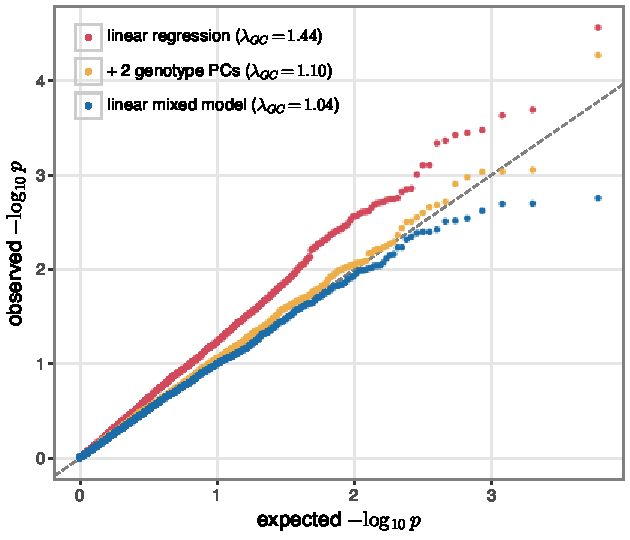
\includegraphics[width=0.55\linewidth]{popstrat_qq.pdf}
  \caption{Quantile-quantile plot of p-values at 3000 null SNPs in a simulated cohort of 1000 people from two populations ($F_{ST}=0.01$), 60\% of them in sibling pairs. The phenotype has heritability 0.5 from 500 causal SNPs elsewhere in the genome, plus a non-genetic difference between the populations. Points above the dashed diagonal indicate inflated test statistics. The relatedness matrix $\mK$ for the LMM and the PCs were computed from 5000 SNPs that exclude the tested SNPs, as in leave-one-chromosome-out analysis.}
  \label{fig:popstrat}
\end{figure}

%======================================================================
\section{Summary statistics}
\label{sec:sumstats}
%======================================================================

\subsection{What and why}

A GWAS is usually reported as \emph{summary statistics}: for every SNP, the estimated effect $\hat\beta_s$, its standard error, the p-value, the alleles and their frequency, and the sample size. Any two of $\hat\beta_s$, $\operatorname{SE}(\hat\beta_s)$, $\hat z_s$ and the p-value (with the sign of the effect) determine the others approximately. Summary statistics have become the main currency of human genetics, for two reasons.
\begin{itemize}
  \item \emph{Sharing.} Individual genotypes and phenotypes are protected by the consent agreements under which they were collected and often cannot leave the institution or country that holds them. Summary statistics usually can be shared and are often public.
  \item \emph{Scale.} Individual-level data for a large GWAS is a matrix of millions of SNPs by hundreds of thousands of people. Summary statistics are a few numbers per SNP.
\end{itemize}
Sharing summary statistics allows \emph{meta-analysis}, combining studies of the same trait in different cohorts. In machine learning terms this is the simplest instance of federated learning, in which models are fitted where the data live and only parameters are pooled. Suppose $K$ cohorts report estimates $\hat\beta_{sk}$ with standard errors $\operatorname{SE}_{sk}$ for the same SNP $s$ and the same true effect $\beta_s$, $k=1,\dots,K$, so that $\hat\beta_{sk}\sim\Normal(\beta_s,\operatorname{SE}_{sk}^2)$ independently. The log likelihood of $\beta_s$ is $-\sum_k(\hat\beta_{sk}-\beta_s)^2/(2\operatorname{SE}_{sk}^2)$ plus a constant, and setting its derivative to zero gives the inverse-variance weighted estimate
\begin{equation}
  \hat\beta_s = \frac{\sum_kw_k\hat\beta_{sk}}{\sum_kw_k},\qquad w_k=\frac1{\operatorname{SE}_{sk}^2},\qquad \operatorname{SE}(\hat\beta_s)=\Bigl(\sum_kw_k\Bigr)^{-1/2}.
\end{equation}
This fixed-effects meta-analysis is what tools such as METAL implement~\citep{willer2010}. There is now a large literature of methods that use only summary statistics, often together with an estimate of the LD between SNPs from a reference panel~\citep{pasaniuc2017}.

\subsection{Summary statistics and LD}

Summary statistics together with the LD matrix carry essentially the same information as the individual-level data for a linear model. To see this, suppose that each column of $\mX\in\R^{N\times P}$ and $\vy$ are standardized to mean zero and variance one, where $\mX$ now holds the $P$ SNPs of one region, and that the phenotype follows a joint linear model in these SNPs,
\begin{equation}
  \vy=\mX\vb+\veps,\qquad\veps\sim\Normal(\mathbf{0},\sigma^2\mI),
\end{equation}
with true joint effects $\vb\in\R^P$. The noise $\veps$ includes the effects of variants elsewhere in the genome, which are unlinked to, and so uncorrelated with, the genotypes in the region. The per-SNP (marginal) least-squares estimate for SNP $j$ is $\hat\beta_j=\mX_{:j}^\top\vy/\mX_{:j}^\top\mX_{:j}=\mX_{:j}^\top\vy/N$. Stacking these into a vector,
\begin{equation}
  \hat\vb = \frac1N\mX^\top\vy = \frac1N\mX^\top\mX\vb + \frac1N\mX^\top\veps = \mR\vb + \frac1N\mX^\top\veps,
\end{equation}
where $\mR=\mX^\top\mX/N\in\R^{P\times P}$ is the matrix of correlations between SNPs, the \emph{LD matrix}, with ones on the diagonal and $R_{jk}=r_{jk}$. Given $\mX$, the noise term has mean zero and covariance $\frac1{N^2}\mX^\top(\sigma^2\mI)\mX=\frac{\sigma^2}N\mR$, so
\begin{equation}
  \hat\vb\sim\Normal\Bigl(\mR\vb,\ \frac{\sigma^2}N\mR\Bigr).
\end{equation}
A single region explains a small fraction of the phenotypic variance, so $\sigma^2\approx1$ and the marginal standard errors are all approximately $\sqrt{1/N}$. Defining the z-scores $\vzh=\sqrt N\hat\vb\in\R^P$ and the \emph{true} (joint) z-scores $\vz=\sqrt N\vb\in\R^P$,
\begin{equation}
  \vzh\sim\Normal(\mR\vz,\ \mR).
  \label{eq:zR}
\end{equation}
The true z-scores are unobserved. One way to think of them is as the expected z-score each SNP would have if it were the only SNP in the model, or, divided by $\sqrt N$, as the joint effect sizes that an infinitely large study would recover.

Equation~\eqref{eq:zR} says that the observed z-scores are the true z-scores \emph{mixed} by LD, plus noise that is itself correlated by LD. Suppose that a region contains a single causal SNP $c$, so that $\vz=z_c\ve_c$, where $\ve_c$ is the $c$-th standard basis vector. Then $\E[\hat z_j]=R_{jc}z_c$: the causal SNP has the largest expected signal, since $R_{cc}=1$, and the signal leaks into every SNP $j$ in proportion to its correlation with $c$. SNPs that are associated only through LD with a causal SNP are called \emph{tag} SNPs. The grey line in Figure~\ref{fig:finemap}a is this expected signal for a simulated locus. Because the noise is also correlated, a tag SNP can by chance have a larger $|\hat z_j|$ than the causal SNP.

Equation~\eqref{eq:zR} can be used as a likelihood, with $\vzh$ the observed data and $\vz$ latent variables to be inferred, and with priors on $\vz$ that may depend on features of each SNP~\citep{hormozdiari2014,zhu2017}. Two caveats apply. The derivation used the LD in the GWAS sample itself (\emph{in-sample} LD); in practice $\mR$ usually comes from a reference panel, and a mismatch between the two can create spurious signals. And $\mR$ is $P\times P$ with $P$ in the millions, but LD decays with distance, so $\mR$ is close to block diagonal and is stored and used one region at a time.

%======================================================================
\section{Fine-mapping}
\label{sec:finemap}
%======================================================================

\emph{Fine-mapping} is the task of identifying the causal variants within an associated locus, as opposed to the many tag SNPs. The usual approach is Bayesian: compute, for each SNP, the posterior probability that it is causal.

\subsection{A single causal variant}

Assume that a locus of $P$ SNPs contains exactly one causal SNP, with unknown index $c\in\{1,\dots,P\}$ and prior $P(c=j)=\pi_j$. Given $c=j$, the true z-scores are $\vz=\lambda\ve_j$, with $\lambda\sim\Normal(0,\omega^2)$ a prior on the causal effect on the z-score scale. Under the model~\eqref{eq:zR}, $\vzh\mid c=j,\lambda\sim\Normal(\lambda\vr_j,\mR)$, where $\vr_j$ is the $j$-th column of $\mR$.

The Bayes factor comparing ``SNP $j$ is causal'' with the null model $\vz=\mathbf{0}$ depends only on $\hat z_j$. To see this, factorize $p(\vzh)=p(\hat z_j)\,p(\vzh_{-j}\mid\hat z_j)$, where $\vzh_{-j}$ denotes the other $P-1$ z-scores. Under $c=j$, $\hat z_j\mid\lambda\sim\Normal(\lambda,1)$ since $R_{jj}=1$. By the conditioning formula for the multivariate Gaussian, the conditional distribution of the others is
\begin{equation}
  \vzh_{-j}\mid\hat z_j,\lambda\sim\Normal\bigl(\lambda\vr_{-j}+\vr_{-j}(\hat z_j-\lambda),\ \mR_{-j,-j}-\vr_{-j}\vr_{-j}^\top\bigr) = \Normal\bigl(\vr_{-j}\hat z_j,\ \mR_{-j,-j}-\vr_{-j}\vr_{-j}^\top\bigr),
\end{equation}
where $\vr_{-j}$ is $\vr_j$ without its $j$-th entry and $\mR_{-j,-j}$ is $\mR$ without row and column $j$. This does not depend on $\lambda$, and it is the same under the null ($\lambda=0$). It therefore cancels in the Bayes factor. Integrating $\lambda$ out of $p(\hat z_j\mid\lambda)$ gives $\hat z_j\sim\Normal(0,1+\omega^2)$ under $c=j$, against $\Normal(0,1)$ under the null, so
\begin{equation}
  \mathrm{BF}_j = \frac{\Normal(\hat z_j;0,1+\omega^2)}{\Normal(\hat z_j;0,1)} = \frac1{\sqrt{1+\omega^2}}\exp\left(\frac{\hat z_j^2}2\,\frac{\omega^2}{1+\omega^2}\right).
  \label{eq:abf}
\end{equation}
This is the approximate Bayes factor of \citet{wakefield2009}, written on the z-score scale: with $\hat\beta_j\sim\Normal(\beta_j,V)$ and prior $\beta_j\sim\Normal(0,W)$, $\omega^2=W/V$. The posterior probability that SNP $j$ is the causal one, its \emph{posterior inclusion probability} (PIP), follows from Bayes' rule:
\begin{equation}
  \mathrm{PIP}_j = P(c=j\mid\vzh) = \frac{\pi_j\mathrm{BF}_j}{\sum_{k=1}^P\pi_k\mathrm{BF}_k}.
  \label{eq:pip}
\end{equation}
A $95\%$ \emph{credible set} is the smallest set of SNPs whose PIPs sum to at least $0.95$~\citep{maller2012}. The single-causal-variant model needs only the marginal z-scores, not $\mR$. Its weakness is the assumption itself: many loci contain several independent signals. Models with multiple causal variants use $\mR$ explicitly, either by enumerating configurations of causal SNPs~\citep{hormozdiari2014} or, in the widely used SuSiE method, by writing $\vb$ as a sum of single-effect vectors, each of which has a single-causal-variant posterior of the form~\eqref{eq:pip}~\citep{wang2020susie}.

\subsection{Functional fine-mapping}

The prior $\pi_j$ need not be uniform. SNPs in regulatory elements of a relevant cell type, or SNPs that change protein sequence, are more likely to be causal. \emph{Functional fine-mapping} sets the prior from annotations of each SNP, for example
\begin{equation}
  \pi_j = \frac{\exp(\vlambda^\top\va_j)}{\sum_{k=1}^P\exp(\vlambda^\top\va_k)},
  \label{eq:annot_prior}
\end{equation}
a softmax over a linear function of an annotation vector $\va_j\in\R^L$ (for example, indicators of the ChromHMM state the SNP falls in, Chapter 6), with weights $\vlambda\in\R^L$. The weights are shared across many loci and learned by maximizing the marginal likelihood across loci (Section~\ref{sec:interpret}). \citet{mahajan2018} fine-mapped type 2 diabetes loci using chromatin states from pancreatic islets, the cell type thought to drive much of the genetic risk. Incorporating the annotations raised the PIPs of variants in islet enhancers and promoters and lowered those of variants in heterochromatin (Figure~\ref{fig:t2d_finemap}).

\begin{figure}[!htbp]
  \centering
  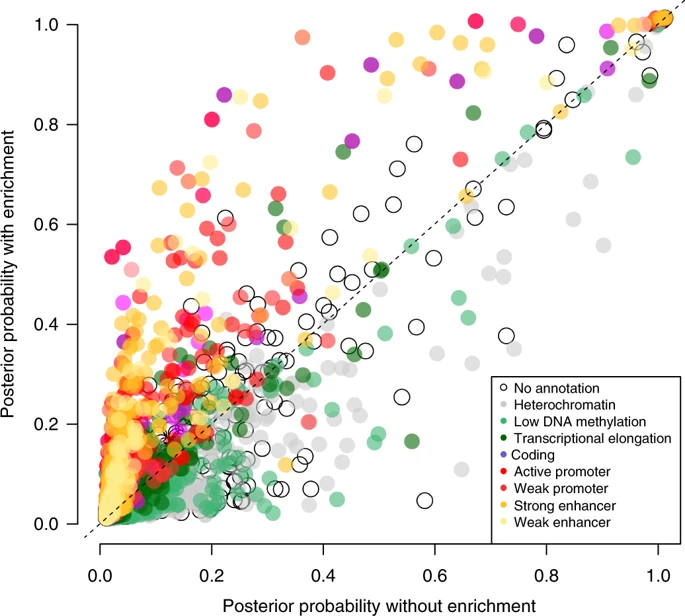
\includegraphics[width=0.5\linewidth]{slides/t2d_functional_finemap.png}
  \caption{Posterior probability that each variant is causal at type 2 diabetes loci, with and without a prior informed by islet chromatin states (colour). Variants in enhancers and promoters move above the diagonal. Reproduced from \citet{mahajan2018}.}
  \label{fig:t2d_finemap}
\end{figure}

Figure~\ref{fig:finemap} shows statistical and functional fine-mapping in a simulated locus. The causal SNP is in an LD block with several others. In this realization, which we chose because it illustrates the point (in most simulations of this locus the lead SNP is the causal one), noise makes a tag SNP the lead SNP. With a uniform prior the causal SNP has PIP 0.23 and the lead SNP 0.50; the 95\% credible set contains five SNPs, including the causal one. With a prior that gives SNPs in annotated elements ten times the weight of others, the causal SNP's PIP rises to 0.71.

\begin{figure}[!htbp]
  \centering
  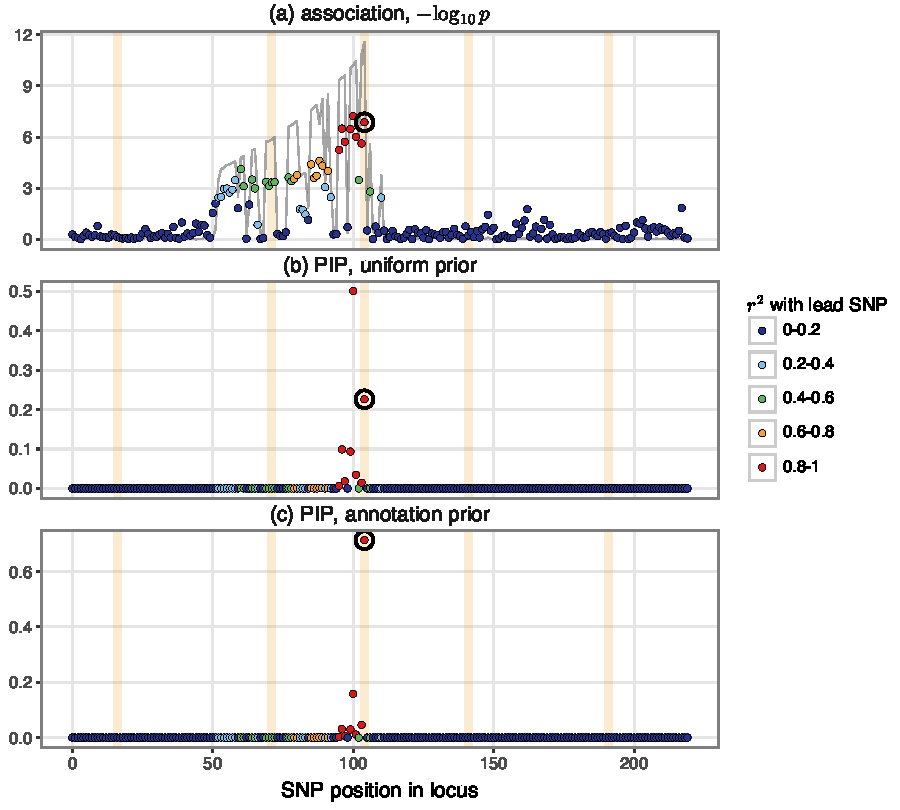
\includegraphics[width=0.9\linewidth]{finemap.pdf}
  \caption{Fine-mapping a simulated locus (5000 individuals, 220 SNPs, three recombination hotspots), with a single causal SNP (ringed) whose true z-score is 7. (a) Marginal association, coloured by $r^2$ with the lead SNP; the grey line is the expected signal $-\log_{10}p$ of $R_{jc}z_c$, showing how the causal signal leaks into correlated SNPs. (b) Posterior inclusion probabilities with a uniform prior, using the Bayes factor~\eqref{eq:abf} with $\omega^2=112.5$. (c) PIPs with prior weight ten times higher for SNPs in annotated elements (shaded), one of which contains the causal SNP.}
  \label{fig:finemap}
\end{figure}

%======================================================================
\section{LD score regression}
\label{sec:ldsc}
%======================================================================

LD score regression~\citep{bulik2015} uses the relation~\eqref{eq:zR} to estimate heritability, and to separate polygenic signal from confounding, using only summary statistics and LD.

\subsection{Derivation}

Take the joint model $\vy=\mX\vb+\veps$ with standardized genotypes and phenotype, and treat the effects as random: $\beta_k$ independent across SNPs with mean zero and variance $h^2/P$, so that the $P$ SNPs together explain heritability $h^2$. From the derivation of~\eqref{eq:zR}, $\vzh=\sqrt N\mR\vb+\ve$ with $\ve\sim\Normal(\mathbf{0},\mR)$ independent of $\vb$, so for SNP $j$
\begin{equation}
  \hat z_j = \sqrt N\sum_{k=1}^PR_{jk}\beta_k + e_j .
\end{equation}
The statistic $\chi^2_j=\hat z_j^2$ has expectation
\begin{equation}
  \E[\chi^2_j] = N\,\E\Bigl[\Bigl(\sum_kR_{jk}\beta_k\Bigr)^2\Bigr] + \E[e_j^2] = N\sum_kR_{jk}^2\Var(\beta_k) + 1 = \frac{Nh^2}P\,\ell_j + 1,
\end{equation}
where the cross term vanishes because $\vb$ and $\ve$ are independent with mean zero, $\E[\beta_k\beta_{k'}]=0$ for $k\neq k'$, $\E[e_j^2]=R_{jj}=1$, and
\begin{equation}
  \ell_j = \sum_{k=1}^P r_{jk}^2
\end{equation}
is the \emph{LD score} of SNP $j$: the sum of its squared correlations with all SNPs, including itself. Since LD is local, the sum is computed in a window around $j$ (1 centimorgan in the original method). Applying~\eqref{eq:zR} to the whole genome glosses over one detail. The noise variance is $1-h^2$ rather than 1, but chance in-sample correlations between unlinked SNPs, of order $1/\sqrt N$ each, add about $h^2$ to $\E[\chi^2_j]$ when summed over the genome, so the constant term is still close to 1. \citet{bulik2015} handle this by noting that a sample $r^2$ has expectation $r^2+(1-r^2)/N$. The intuition is that a SNP's $\chi^2$ collects signal from every causal variant it tags, in proportion to $r^2$, so under polygenicity SNPs with high LD scores have larger $\chi^2$ on average (Figure~\ref{fig:ldscore_schematic}).

\begin{figure}[!htbp]
  \centering
  \begin{tikzpicture}[every node/.style={font=\small}, >=Stealth]
    \draw[thick] (0,0) -- (10,0);
    \foreach \x in {0.6,1.4,2.2,3.0,3.8,5.0,6.2,7.0,7.8,8.6,9.4} \fill[gray] (\x,0) circle (2pt);
    \fill[black] (5.0,0) circle (3pt) node[below=3pt] {$j$};
    \foreach \x/\i/\h in {2.2/1/1.3, 6.2/2/0.6, 8.6/3/1.2}
      {\fill[red!70!black] (\x,0) circle (3pt); \node[below=3pt] at (\x,0) {$k=\i$};
       \draw[->, red!70!black, thick] (\x,0.1) .. controls (\x,\h) and (5.0,\h) .. (5.0,0.12);
       \node[red!70!black, above] at ({(\x+5.0)/2},{0.75*\h}) {$r_{j\i}^2$};}
    \node[above] at (5.0,1.75) {$\chi^2_j$ collects signal from every SNP $k$ in LD with $j$};
  \end{tikzpicture}
  \caption{Intuition for LD scores. The test statistic at SNP $j$ (black) includes signal from the causal SNPs $k$ it is correlated with (red), each weighted by $r_{jk}^2$. Under polygenicity every SNP has a small effect, so $\E[\chi_j^2]$ grows with $\ell_j=\sum_kr_{jk}^2$.}
  \label{fig:ldscore_schematic}
\end{figure}

Confounding by population structure or cryptic relatedness adds a bias term $\sqrt Nb_j$ to $\hat z_j$, where $b_j$ reflects the correlation between SNP $j$ and the confounder. Let $a=\E[b_j^2]$. Allele frequency differences between populations arise from genetic drift at each SNP and are not systematically larger at SNPs with high LD scores, so to a good approximation $a$ does not depend on $\ell_j$, giving
\begin{equation}
  \E[\chi^2_j] = \frac{Nh^2}P\,\ell_j + Na + 1 .
  \label{eq:ldsc}
\end{equation}
This is a linear regression of $\chi^2_j$ on $\ell_j$ across SNPs, with slope $Nh^2/P$ and intercept $1+Na$. The $\chi^2_j$ come from summary statistics, $N$ is known and $\ell_j$ is computed from a reference panel, so fitting the regression estimates $h^2$ from the slope and the amount of confounding from the intercept. Inflation due to polygenicity increases with LD score; inflation due to confounding does not. In practice the regression is weighted to account for the heteroskedasticity and correlation of the $\chi^2_j$, and standard errors are estimated with a block jackknife over the genome.

Figure~\ref{fig:ldsc} applies~\eqref{eq:ldsc} to simulated summary statistics. Without confounding, $\lambda_{GC}=1.56$ although there is no confounding at all, and LD score regression gives an intercept of 1.00 and recovers $h^2=0.5$. With population stratification, the intercept rises to 1.27 (the value implied by the simulation is 1.24) while the slope, and so the heritability estimate, changes little.

\begin{figure}[!htbp]
  \centering
  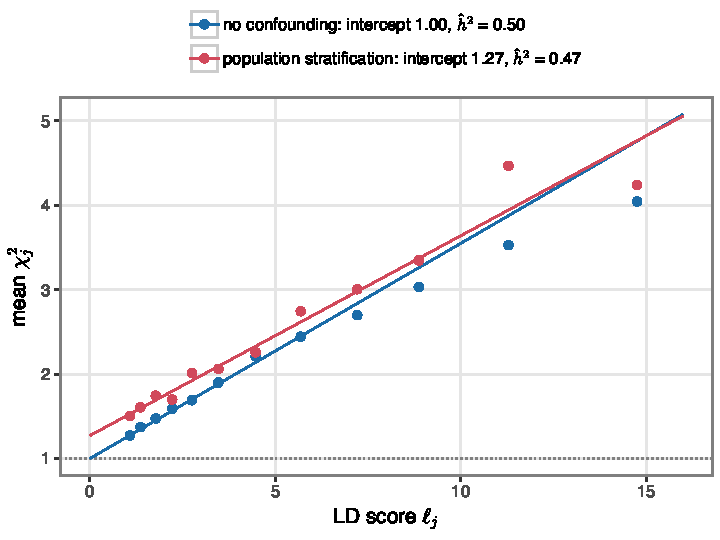
\includegraphics[width=0.6\linewidth]{ldsc.pdf}
  \caption{LD score regression on simulated summary statistics for 98{,}000 SNPs, $N=50{,}000$ and $h^2=0.5$, generated from $\vzh=\sqrt N\mR\vb+\ve$ with $\mR$ from simulated haplotypes in 4000 regions of varying LD. Points are mean $\chi^2$ in bins of LD score, lines the least-squares fits to all SNPs. Stratification was simulated by adding a term proportional to each SNP's allele frequency difference between two populations.}
  \label{fig:ldsc}
\end{figure}

\subsection{Stratified LD score regression}

The same argument partitions heritability by functional annotation~\citep{finucane2015}. Let $C_1,\dots,C_M$ be sets of SNPs defined by annotations (coding, promoter, enhancer in a given tissue, and so on), which may overlap, and let the variance of each effect depend on the annotations of its SNP,
\begin{equation}
  \beta_k\sim\Normal\Bigl(0,\ \sum_{c=1}^M\tau_c\ind[k\in C_c]\Bigr),
\end{equation}
where $\tau_c$ is the per-SNP contribution to heritability of annotation $c$. Repeating the derivation,
\begin{equation}
  \E[\chi^2_j] = N\sum_kR_{jk}^2\sum_c\tau_c\ind[k\in C_c] + Na+1 = N\sum_{c=1}^M\tau_c\,\ell(j,c) + Na + 1,\qquad \ell(j,c)=\sum_{k\in C_c}r_{jk}^2,
\end{equation}
where $\ell(j,c)$ is the LD score of SNP $j$ with respect to annotation $c$: how much of the signal that SNP $j$ picks up comes from SNPs in $C_c$. Fitting this multiple regression of $\chi^2_j$ on the $M$ annotation-specific LD scores estimates the $\tau_c$. The heritability in annotation $c$ is $h^2(C_c)=\sum_{k\in C_c}\Var(\beta_k)$, and its \emph{enrichment} is the fraction of heritability in $C_c$ divided by the fraction of SNPs in $C_c$. \citet{finucane2015} fitted a baseline model of several dozen annotations, including coding, UTR, promoter and enhancer regions and conserved sequence. Regions conserved across mammals, which contain about 2.6\% of common SNPs, were the most enriched, explaining about a third of the heritability averaged across traits. The model also gives a principled test of tissue specificity (Section~\ref{sec:interpret}).

A cross-trait version regresses the product $\hat z_{1j}\hat z_{2j}$ of z-scores for two traits on $\ell_j$ to estimate their \emph{genetic correlation}~\citep{bulik2015b}. Schizophrenia, bipolar disorder and major depression, for example, are genetically correlated: variants that raise risk for one tend to raise risk for the others.

%======================================================================
\section{Interpreting GWAS associations}
\label{sec:interpret}
%======================================================================

\subsection{Most associations are non-coding}

A variant that changes the amino acid sequence of a protein points directly at a gene and suggests a mechanism. Most GWAS associations, however, lie in introns or between genes~\citep{hindorff2009}, and presumably act by changing how much of a gene is expressed, when and where, or how it is spliced. This makes them harder to interpret: the variant, the cell type in which it acts and the gene it regulates are all unknown.

\citet{pickrell2014} estimated the contribution of different classes of variant by fitting a hierarchical model to the summary statistics of 18 traits. The genome is split into regions $k$, each containing a set $S_k$ of SNPs and assumed to contain at most one causal variant. The model has two levels. The prior probability $\Pi_k$ that region $k$ contains an association depends on region-level features $I_{kl}$ (such as gene density), and given an association, the probability $\pi_{ik}$ that SNP $i$ is the causal one depends on SNP-level annotations $I_{il}$ (such as falling in a coding exon or in a DNase I hypersensitive site in some cell type):
\begin{equation}
  \logit(\Pi_k)=\log\frac{\Pi_k}{1-\Pi_k} = \kappa+\sum_{l=1}^{L_1}\gamma_lI_{kl},\qquad
  \pi_{ik} = \frac{e^{x_i}}{\sum_{j\in S_k}e^{x_j}},\quad x_i=\sum_{l=1}^{L_2}\lambda_lI_{il},
\end{equation}
where $\kappa$ is an intercept, $\gamma_l$ are the coefficients of the $L_1$ region-level features and $\lambda_l$ those of the $L_2$ SNP-level annotations. The second level is the functional prior~\eqref{eq:annot_prior}. Which SNP is causal is never observed, so the model is fitted by maximizing the marginal likelihood. By the law of total probability, the probability of the data $\mathcal{D}_k$ in region $k$ is $(1-\Pi_k)\,p(\mathcal{D}_k\mid\text{null})+\Pi_k\sum_{i\in S_k}\pi_{ik}\,p(\mathcal{D}_k\mid\text{SNP $i$ causal})$. Dividing by $p(\mathcal{D}_k\mid\text{null})$, which does not depend on the parameters, and using the Bayes factors~\eqref{eq:abf} gives the likelihood relative to the null,
\begin{equation}
  L_k(\kappa,\vgamma,\vlambda) = (1-\Pi_k) + \Pi_k\sum_{i\in S_k}\pi_{ik}\mathrm{BF}_i,
\end{equation}
and the parameters maximize $\sum_k\log L_k$. Once fitted, the model gives each region's posterior probability of containing an association and each SNP's PIP, from which the fraction of associations attributable to coding variants follows. That fraction ranged from a few percent to about 20\% across traits (Figure~\ref{fig:pickrell}a): the large majority of the signal is non-coding.

\subsection{Which tissues?}

If a trait's heritability is concentrated in regulatory elements active in one tissue, that tissue is likely to be where the causal variants act. Stratified LD score regression tests this directly: add an annotation of the regulatory elements of one cell type (for example, regions marked by the enhancer-associated histone modifications H3K27ac or H3K4me1 in Roadmap Epigenomics data, Chapter 3) to the baseline model and test whether its coefficient $\tau_c$ is positive. Controlling for the baseline annotations matters, because regulatory elements in every tissue are enriched for heritability compared with the genome as a whole. Figure~\ref{fig:pickrell}b shows the results for ten groups of cell types~\citep{finucane2015}. Most make biological sense: central nervous system (CNS) elements for schizophrenia and bipolar disorder, immune cells for rheumatoid arthritis and Crohn's disease, connective tissue and bone for height, liver for HDL cholesterol. BMI is enriched in CNS, consistent with a role for appetite and behaviour, as are years of education and smoking. The \textit{FTO} example below shows that adipose tissue matters for BMI too.

\begin{figure}[!htbp]
  \centering
  \begin{subfigure}[b]{\linewidth}
    \centering
    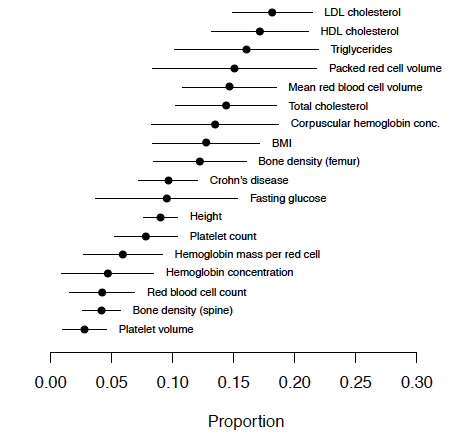
\includegraphics[width=0.45\linewidth]{slides/coding_fraction.png}
    \caption{}
  \end{subfigure}\\[4pt]
  \begin{subfigure}[b]{\linewidth}
    \centering
    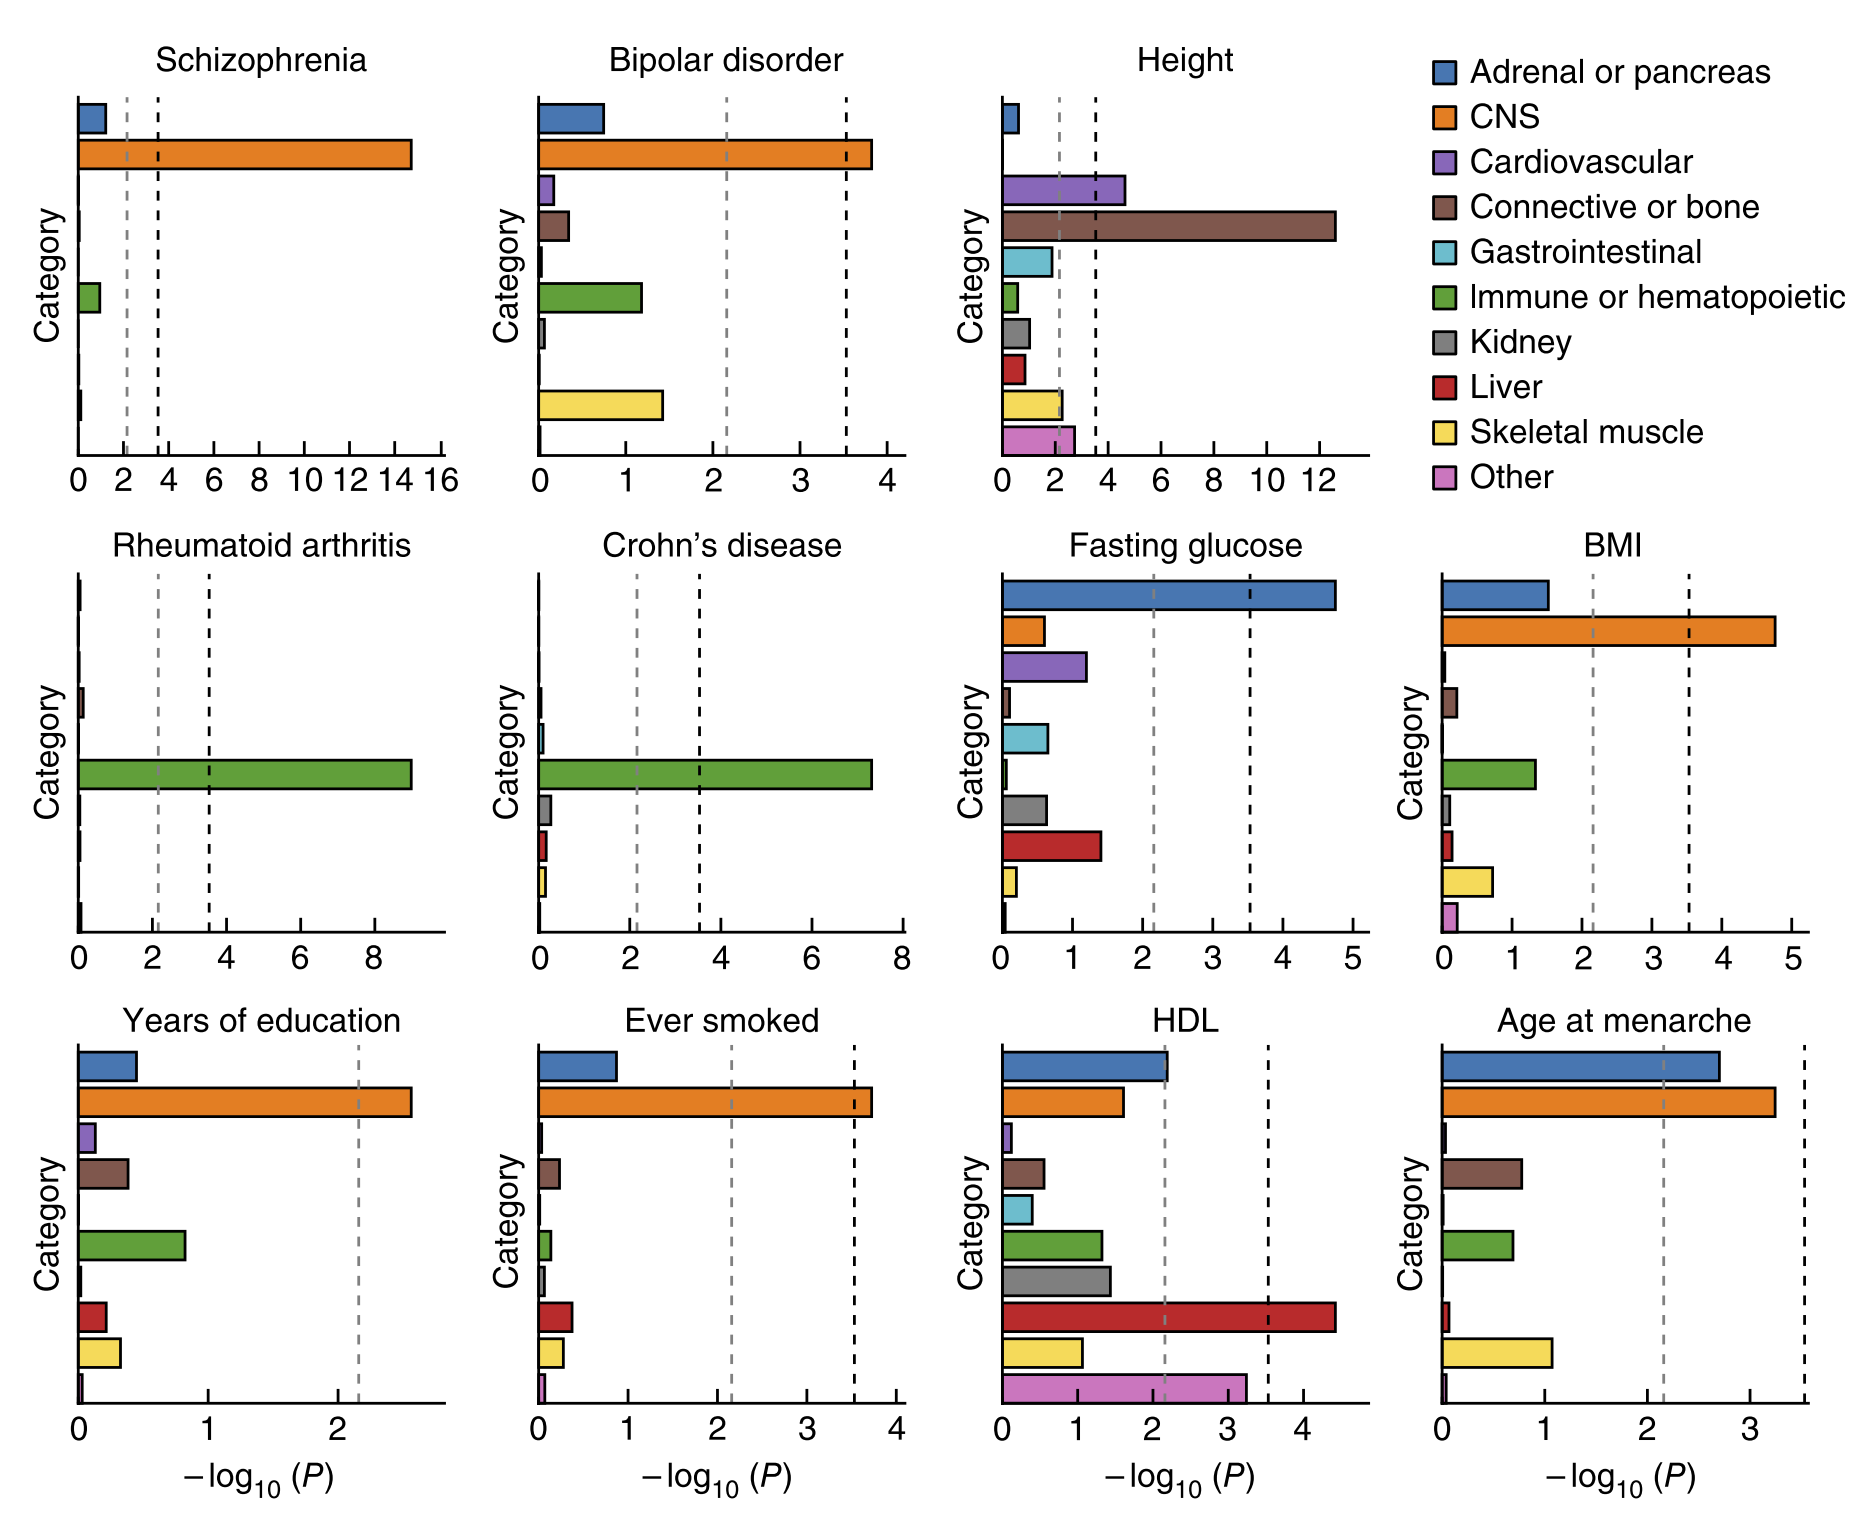
\includegraphics[width=0.85\linewidth]{slides/tissue_enrichment.png}
    \caption{}
  \end{subfigure}
  \caption{(a) Estimated proportion of association signals due to non-synonymous (coding) variants for 18 traits, with confidence intervals. Reproduced from \citet{pickrell2014}. (b) Enrichment of heritability in regulatory elements of ten groups of cell types, estimated by stratified LD score regression, for twelve traits. Bars are $-\log_{10}p$ for a positive coefficient $\tau_c$; dashed lines are multiple-testing thresholds. Reproduced from \citet{finucane2015}.}
  \label{fig:pickrell}
\end{figure}

\subsection{Other routes to interpretation}

Annotation overlap is one of several tools for interpreting GWAS loci. Sequence-to-function models such as those of Chapters 2 and 3 predict the effect of each variant on chromatin accessibility or expression, by in silico mutagenesis (Chapter 4), and these predictions can serve as annotations $\va_j$. Molecular quantitative trait loci, genetic associations with molecular phenotypes such as gene expression, connect variants to genes and cell types directly; they are the subject of the next chapter.

%======================================================================
\section{Case study: the \textit{FTO} obesity locus}
\label{sec:fto}
%======================================================================

The strongest common-variant association with obesity, in both adults~\citep{frayling2007} and children~\citep{bradfield2012}, lies in the first introns of the gene \textit{FTO} on chromosome 16 (Figure~\ref{fig:fto_locus}A). It is a typical GWAS locus: dozens of SNPs in strong LD, in a non-coding region, with several genes nearby. For years it was assumed that the variants act through \textit{FTO}, simply because they lie inside it. \citet{claussnitzer2015} worked through the locus systematically, using many of the ideas of this book, and the story is one of the clearest dissections of a GWAS association.

\paragraph{Cell type.} Chromatin states inferred by ChromHMM (Chapter 6) across 127 Roadmap reference epigenomes showed that the region of strongest association is in an enhancer state in mesenchymal cells, a class that includes adipocyte (fat cell) progenitors, and not in most other cell types (Figure~\ref{fig:fto_locus}B). In a luciferase reporter assay, which measures how strongly a DNA segment drives expression of a reporter gene, one 10-kb segment carrying the risk haplotype had more than twice the enhancer activity of the non-risk haplotype (Figure~\ref{fig:fto_locus}C).

\paragraph{Target genes.} The enhancer could regulate any gene within reach. Hi-C data (Chapter 3) showed long-range contacts in pre-adipocytes between the risk region and promoters up to about a megabase away (Figure~\ref{fig:fto_genes}c), consistent with earlier evidence of contacts with \textit{IRX3} in other cell types~\citep{smemo2014}. Comparing expression between people carrying the risk and non-risk genotypes, in pre-adipocytes, showed no difference for \textit{FTO} itself but higher expression of \textit{IRX3} and \textit{IRX5}, which lie about 0.5 and 1.2 Mb away (Figure~\ref{fig:fto_genes}b). The effect was specific to pre-adipocytes. The obvious culprit, \textit{FTO}, appears innocent here; in many other loci, though, the nearest gene is the causal one.

\begin{figure}[!htbp]
  \centering
  \begin{subfigure}[b]{\linewidth}
    \centering
    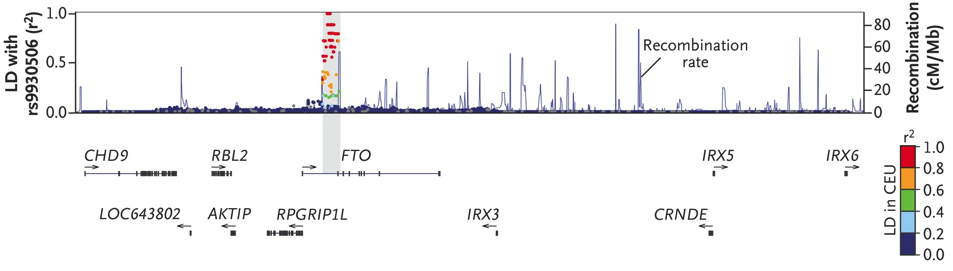
\includegraphics[width=0.85\linewidth]{slides/fto_region.png}
    \caption{}
  \end{subfigure}\\[2pt]
  \begin{subfigure}[b]{\linewidth}
    \centering
    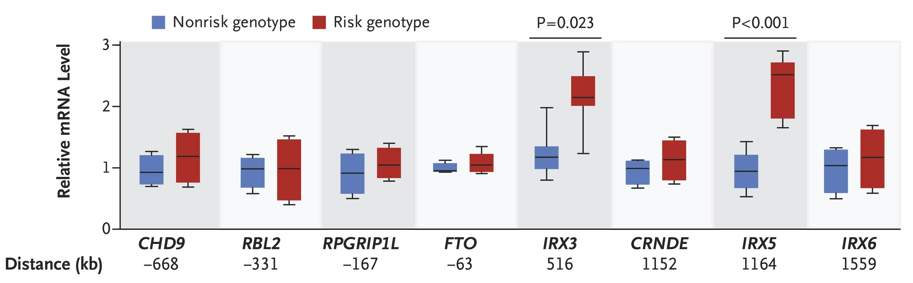
\includegraphics[width=0.85\linewidth]{slides/fto_expression.png}
    \caption{}
  \end{subfigure}\\[2pt]
  \begin{subfigure}[b]{\linewidth}
    \centering
    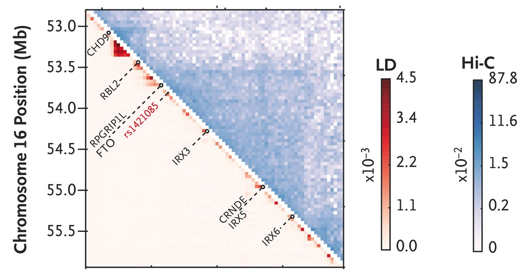
\includegraphics[width=0.55\linewidth]{slides/fto_hic.png}
    \caption{}
  \end{subfigure}
  \caption{Target genes of the \textit{FTO} risk locus. (a) The 2.5-Mb region around the locus, with genes; points show LD with the lead SNP rs9930506 and the blue line the recombination rate. The LD block (grey) is confined to \textit{FTO}. (b) Expression of genes in the region in human pre-adipocytes from carriers of the risk and non-risk genotypes, with distance from the risk variant; only \textit{IRX3} and \textit{IRX5} differ. (c) LD (lower triangle, red) and Hi-C contact frequency in pre-adipocytes (upper triangle, blue) across the region; the risk variant rs1421085 contacts distant promoters although LD does not extend to them. Reproduced from \citet{claussnitzer2015}.}
  \label{fig:fto_genes}
\end{figure}

\paragraph{Causal variant and mechanism.} Using conservation and the predicted disruption of transcription factor binding motifs to prioritize among the SNPs in the block, \citet{claussnitzer2015} identified rs1421085 as the likely causal variant: its risk allele (C instead of T) disrupts a binding motif for the repressor ARID5B, derepressing the enhancer and raising \textit{IRX3} and \textit{IRX5} expression. Higher \textit{IRX3} and \textit{IRX5} expression shifts the fate of adipocyte progenitors away from \emph{beige} adipocytes, which burn lipids to produce heat (thermogenesis), toward \emph{white} adipocytes, which store lipids. Editing the risk allele to the non-risk allele with CRISPR-Cas9 in adipocyte progenitors from risk-allele carriers restored thermogenesis. A tendency to store rather than burn energy was probably advantageous when food was scarce and is maladaptive when it is abundant.

The \textit{FTO} story uses most of the steps that are now standard in interpreting a GWAS locus: fine-mapping within the LD block, chromatin state annotations to find the relevant cell type, chromatin contacts and expression differences between genotypes to find the target genes, sequence motifs to find the causal variant, and experiments to confirm the mechanism. It also suggests possible interventions, for example reducing \textit{IRX3} or \textit{IRX5} activity in adipocyte progenitors.

%======================================================================
\section{Summary}
%======================================================================

\begin{itemize}
  \item Humans differ at millions of sites, mostly SNPs. Most SNPs are rare, but most of the differences between two people are at common SNPs.
  \item Mendelian diseases are caused by variants in single genes; complex traits are influenced by thousands of variants of small effect together with environment. Large-effect variants tend to be rare, because of negative selection and because rare variants are detected only when their effects are large.
  \item A GWAS regresses the phenotype on each SNP's dosage separately and calls associations at $p<5\times10^{-8}$.
  \item Recombination breaks up the correlation between nearby variants slowly, $D_t=(1-c)^tD_0$, leaving LD blocks between hotspots. LD allows imputation of unmeasured SNPs from reference panels, with hidden Markov models, but makes the causal variant within a block hard to identify.
  \item Population structure and relatedness confound association tests. Genotype PCs correct for broad ancestry; linear mixed models with a realized relatedness matrix correct for both, and an eigendecomposition makes them fast.
  \item Summary statistics are easy to share and meta-analyse. Under a linear model, marginal z-scores satisfy $\vzh\sim\Normal(\mR\vz,\mR)$: the true signal is mixed by LD.
  \item Fine-mapping computes posterior inclusion probabilities and credible sets; under a single causal variant they depend only on the marginal z-scores. Functional annotations sharpen them through the prior.
  \item LD score regression, $\E[\chi^2_j]=Nh^2\ell_j/P+Na+1$, separates polygenicity (slope) from confounding (intercept), and its stratified form partitions heritability across annotations and tissues.
  \item Most associations are non-coding and act through gene regulation in specific cell types; finding the causal variant, cell type and gene, as at \textit{FTO}, remains the central task after a GWAS.
\end{itemize}

%======================================================================
\section*{Exercises}
%======================================================================

\begin{enumerate}
  \item Show that for two loci, $D=f_{AB}f_{ab}-f_{Ab}f_{aB}$, where the four terms are haplotype frequencies. If $c=0.01$, how many generations does it take for $D$ to halve?
  \item Under Hardy--Weinberg equilibrium, show that $\Var(x_{is})=2f_s(1-f_s)$. For $N=500{,}000$, what per-allele effect gives 80\% power at $p<5\times10^{-8}$ for a SNP with MAF 1\%? Use the non-centrality parameter of about 40.
  \item Derive the profile log likelihood of $\delta$ for the LMM by substituting $\hat\vtheta$ and $\hat\sigma_g^2$ into~\eqref{eq:lmm_ll}, and write it in terms of the eigenvalues of $\mK$ and the rotated data.
  \item Suppose a locus contains two SNPs with correlation $r$, one of which is causal with true z-score $z$. Using~\eqref{eq:zR}, find the probability that the non-causal SNP has the larger $|\hat z|$ as a function of $r$ and $z$, and evaluate it for $r=0.95$, $z=6$.
  \item Show that inverse-variance weighted meta-analysis of $K$ cohorts gives the same $\hat\beta$ as pooling the data into one regression when there are no covariates, the genotypes are centered within each cohort and the noise variance is the same in every cohort.
  \item Extend the LD score regression derivation to two traits measured in the same individuals, with genetic covariance $\rho_g$ between the effects $\beta_{1k}$ and $\beta_{2k}$ and phenotypic correlation $\rho$, and find $\E[\hat z_{1j}\hat z_{2j}]$.
  \item Implement the single-causal-variant fine-mapping of Section~\ref{sec:finemap}, apply it to the simulated locus in \texttt{make\_figures.py}, and study how the size of the 95\% credible set changes with $N$ and with the LD around the causal SNP.
\end{enumerate}

\bibliographystyle{abbrvnat}
\bibliography{../chapter11/chapter11}
\endgroup

% Generated wrapper: chapter 12 with its own figure path, macros and bibliography.
\graphicspath{{../chapter12/figures/}}
\makeatletter\def\input@path{{../chapter12/}}\makeatother
\begingroup
% Chapter 12: molecular quantitative trait loci.
% Requires: amsmath, amssymb, bm, graphicx, booktabs, multirow, subcaption,
% tikz (arrows.meta, positioning, calc, decorations.pathreplacing, decorations.pathmorphing, shapes.geometric, fit), natbib.
% Computed figures are produced by scripts/make_figures.py; figures/slides/ holds figures taken from the lecture slides.

\providecommand{\R}{\mathbb{R}}
\providecommand{\E}{\mathbb{E}}
\providecommand{\Normal}{\mathcal{N}}
\providecommand{\argmax}{\operatorname*{arg\,max}}
\providecommand{\argmin}{\operatorname*{arg\,min}}
\providecommand{\vy}{\mathbf{y}}
\providecommand{\vx}{\mathbf{x}}
\providecommand{\mX}{\mathbf{X}}
\providecommand{\mI}{\mathbf{I}}
\providecommand{\vb}{\boldsymbol{\beta}}
\providecommand{\veps}{\boldsymbol{\epsilon}}
\providecommand{\vp}{\mathbf{p}}
\providecommand{\vg}{\mathbf{g}}
\providecommand{\ind}{\mathbf{1}}
% new in this chapter
\providecommand{\mY}{\mathbf{Y}}
\providecommand{\mW}{\mathbf{W}}
\providecommand{\mE}{\mathbf{E}}
\providecommand{\mS}{\mathbf{S}}
\providecommand{\mF}{\mathbf{F}}
\providecommand{\mG}{\mathbf{G}}
\providecommand{\mR}{\mathbf{R}}
\providecommand{\mU}{\mathbf{U}}
\providecommand{\mV}{\mathbf{V}}
\providecommand{\mD}{\mathbf{D}}
\providecommand{\mA}{\mathbf{A}}
\providecommand{\mSigma}{\boldsymbol{\Sigma}}
\providecommand{\vw}{\mathbf{w}}
\providecommand{\vz}{\mathbf{z}}
\providecommand{\va}{\mathbf{a}}
\providecommand{\vs}{\mathbf{s}}
\providecommand{\vf}{\mathbf{f}}
\providecommand{\vbhat}{\hat{\mathbf{b}}}
\providecommand{\vbb}{\mathbf{b}}
\providecommand{\vm}{\mathbf{m}}
\providecommand{\ve}{\mathbf{e}}
\providecommand{\vlambda}{\boldsymbol{\lambda}}
\providecommand{\vzero}{\mathbf{0}}
\providecommand{\diag}{\operatorname{diag}}
\providecommand{\Gam}{\operatorname{Gamma}}
\providecommand{\Var}{\operatorname{Var}}
\providecommand{\Cov}{\operatorname{Cov}}
\providecommand{\Bin}{\operatorname{Bin}}
\providecommand{\BetaBin}{\operatorname{BetaBin}}
\providecommand{\NB}{\operatorname{NB}}
\providecommand{\Pois}{\operatorname{Pois}}
\providecommand{\BetaDist}{\operatorname{Beta}}
\providecommand{\BetaFn}{\mathrm{B}}

\chapter{Molecular quantitative trait loci}
\label{ch:molqtl}

Chapter 11 showed that genome-wide association studies (GWAS) have found tens of thousands of genomic regions associated with traits and diseases, and that most of the associated variants do not change the sequence of a protein. They are thought to act by changing gene regulation: when, where and how much a gene is expressed or how its RNA is spliced. This chapter is about the main tool for studying that regulation in human populations, the \emph{molecular quantitative trait locus} (molecular QTL): a genetic variant associated with a molecular phenotype such as the expression level of a gene. We cover how molecular QTL studies are designed and analysed, how to remove the hidden confounders that plague large omics data sets, how allele-specific measurements give a second, better controlled view of the same genetic effects, what the large tissue atlases have taught us, and finally how molecular QTLs are combined with GWAS to propose causal genes, using colocalization, transcriptome-wide association studies and Mendelian randomization.

%======================================================================
\section{From GWAS loci to molecular mechanisms}
%======================================================================

\subsection{The FTO locus}

The strongest common genetic association with obesity, in adults and in children~\citep{bradfield2012}, lies in a region of chromosome 16 that contains the gene \textit{FTO}. The associated variants fall in an intron of \textit{FTO}, so the locus was named after it and \textit{FTO} was assumed to be the causal gene. \citet{claussnitzer2015} worked through this locus in detail, and their analysis uses many of the ideas of this and earlier chapters, so it is a good place to start.

Figure~\ref{fig:fto_locus-12}a is a LocusZoom plot of the association with body mass index (BMI). Many variants are strongly associated, and their colour, the linkage disequilibrium (LD) $r^2$ with the lead variant, shows that they are all correlated with each other: genetic association alone cannot say which of them is causal (Chapter 11). The authors next looked at chromatin states from the Roadmap Epigenomics project, the ChromHMM annotation of Chapter 6, across many cell types (Figure~\ref{fig:fto_locus-12}b). The associated region is in an active, enhancer-like state in mesenchymal cells, the progenitors of connective tissue that include adipocytes (fat cells) and their precursors, and much less active elsewhere. That points to adipocyte progenitors as the cell type in which the variants act.

\begin{figure}[!htbp]
  \centering
  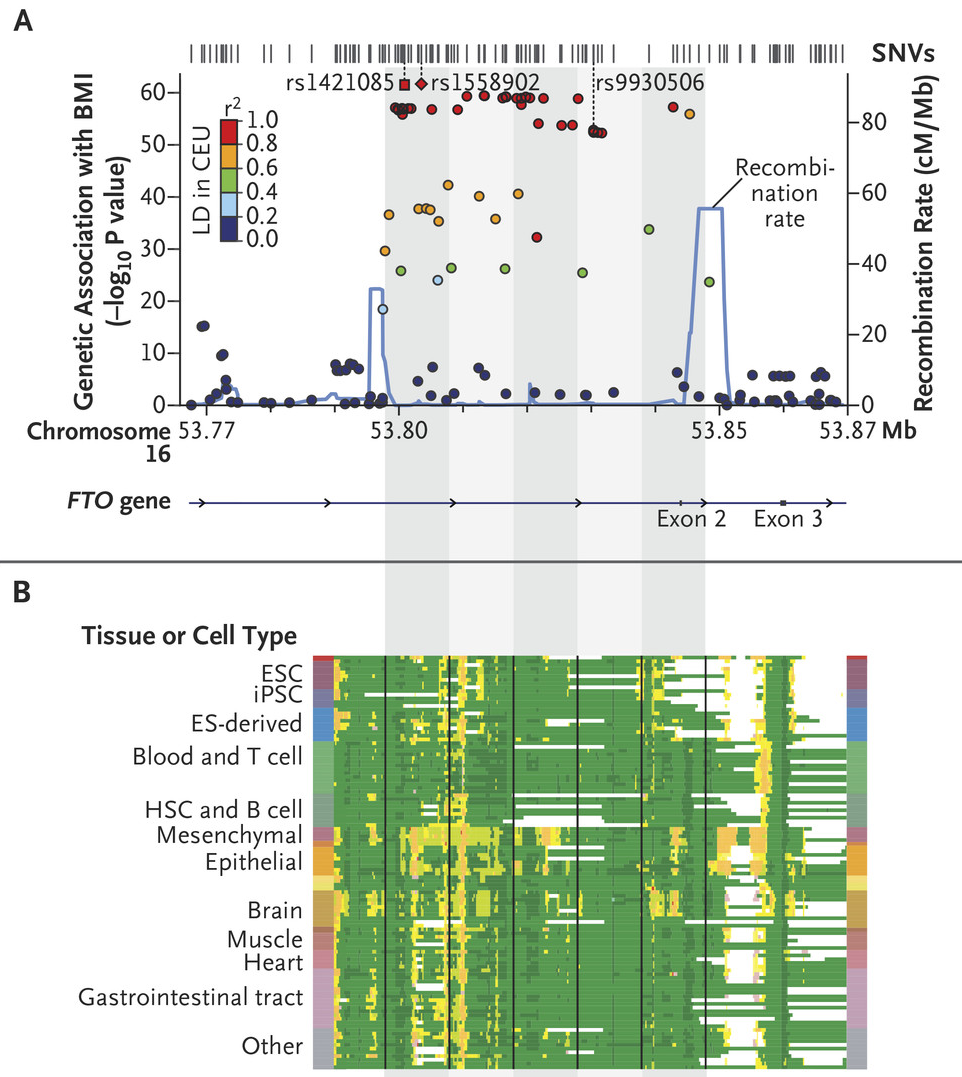
\includegraphics[width=0.72\linewidth]{slides/fto_locus.png}
  \caption{The \textit{FTO} obesity locus. (a) Association of variants with BMI ($-\log_{10}$ p value) along chromosome 16, coloured by LD ($r^2$ in European-ancestry samples) with the lead variants, with the recombination rate and the \textit{FTO} gene below. (b) Roadmap Epigenomics chromatin states across tissues and cell types for the same region; the associated region is in an active enhancer state (yellow) in mesenchymal cells. Reproduced from \citet{claussnitzer2015}.}
  \label{fig:fto_locus-12}
\end{figure}

Which gene does the enhancer regulate? The region contains several genes besides \textit{FTO} (Figure~\ref{fig:fto_expression}, top). In pre-adipocytes from people with the risk and non-risk genotypes, expression of \textit{FTO} itself did not differ, but expression of \textit{IRX3} and \textit{IRX5}, which lie 0.5 and 1.2 megabases (Mb) away, was higher with the risk genotype (Figure~\ref{fig:fto_expression}, bottom). The effect was specific to pre-adipocytes. \textit{IRX3} and \textit{IRX5} encode transcription factors that shift the fate of adipocyte progenitors: higher expression makes a progenitor more likely to become a white adipocyte, which stores lipid, and less likely to become a beige adipocyte, which burns lipid to produce heat (thermogenesis). The risk allele therefore tilts the balance toward fat storage. The authors identified a single nucleotide variant, rs1421085, that disrupts a binding site for the repressor ARID5B, and showed that editing it with CRISPR switched the expression of \textit{IRX3} and \textit{IRX5} and the thermogenic programme. Storing more fat may have been advantageous when food was scarce; in an environment with abundant food the same variant is maladaptive.

\begin{figure}[!htbp]
  \centering
  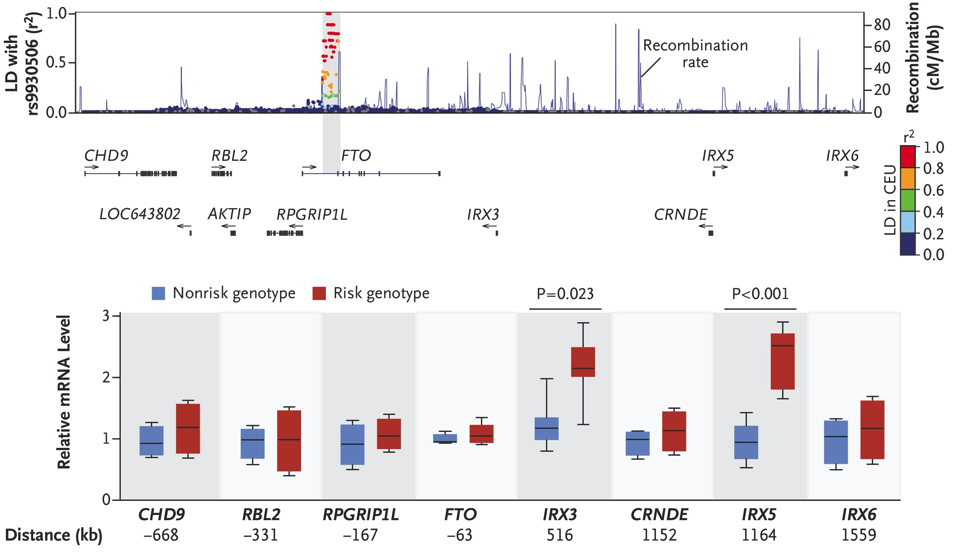
\includegraphics[width=0.85\linewidth]{slides/fto_expression.png}
  \caption{Genes near the \textit{FTO} association (top; LD with the lead variant rs9930506 and recombination rate) and their expression in human pre-adipocytes from carriers of the risk and non-risk genotypes (bottom). Only \textit{IRX3} and \textit{IRX5}, more than 500 kb from the associated variants, differ. Distances are from the associated region. Reproduced from \citet{claussnitzer2015}.}
  \label{fig:fto_expression}
\end{figure}

The example illustrates three general difficulties of interpreting a GWAS locus, which recur throughout this chapter: finding the \emph{causal variant} among many correlated ones, finding the \emph{cell type} (and possibly the cell state) in which it acts, and finding the \emph{target gene}, which need not be the nearest gene. It also shows why we care. Knowing that the locus acts through \textit{IRX3} and \textit{IRX5} in adipocyte progenitors suggests interventions, such as reducing their activity to favour beige adipocytes, and more generally tells us about the human biology of a disease without a clinical trial.

\subsection{Molecular mediators of genetic effects}

The logic of the \textit{FTO} analysis is that of mediation (Figure~\ref{fig:mediation}). A genetic variant is associated with disease risk, and we want to find the molecular changes, such as a change in the expression of a gene, that lie on the causal path between them. Genetic variation is useful here because it gives us one route to causality: genotypes are fixed at conception, so an association between a variant and a molecular trait cannot be caused by the trait. The reverse arrows in Figure~\ref{fig:mediation} are a reminder that the data do not have to follow the simple chain. A variant can raise disease risk through some other route, and the disease can then change gene expression as the body responds to it, so an association between disease and expression measured in patients need not be causal for the disease.

\begin{figure}[!htbp]
  \centering
  \begin{tikzpicture}[>=Stealth, every node/.style={font=\small}, box/.style={draw, rounded corners, minimum width=2.6cm, minimum height=0.8cm, align=center}]
    \node[box, fill=green!12] (g) {genetic variant};
    \node[box, fill=blue!10, right=1.6cm of g] (m) {molecular change\\(e.g.\ expression)};
    \node[box, fill=red!10, right=1.6cm of m] (d) {disease risk};
    \draw[->, thick] ([yshift=3pt]g.east) -- ([yshift=3pt]m.west);
    \draw[->, thick] ([yshift=3pt]m.east) -- ([yshift=3pt]d.west);
    \draw[->, dashed, gray] ([yshift=-3pt]d.west) -- ([yshift=-3pt]m.east) node[midway, below] {reverse};
    \draw[->, dashed, gray] (g.south) to[out=-25, in=-155] node[midway, below] {other paths} (d.south);
  \end{tikzpicture}
  \caption{Molecular mediators of genetic effects. We would like to find molecular changes on the causal path from a variant to disease. Disease can also change molecular phenotypes (reverse causation), and a variant can affect disease through other paths.}
  \label{fig:mediation}
\end{figure}

%======================================================================
\section{Molecular QTLs}
%======================================================================

\subsection{Layers of omics}

Any molecular readout that can be measured at scale across many individuals can be associated with genotype. The readouts follow the layers of gene regulation met in earlier chapters:
\begin{itemize}
  \item the \emph{genome}: the genetic variants themselves;
  \item the \emph{epigenome}: transcription factor binding (ChIP-seq), DNA methylation (bisulfite sequencing or, more cheaply and at larger scale, methylation arrays), chromatin accessibility (ATAC-seq, DNase-seq) and histone modifications;
  \item the \emph{transcriptome}: gene expression and splicing (RNA-seq);
  \item the \emph{proteome}: protein levels, now measured for a few thousand proteins in tens of thousands of people with affinity-based assays;
  \item the \emph{metabolome}: small molecules in cells or blood.
\end{itemize}
A QTL for each readout gets its own name (Table~\ref{tab:qtl_types}). The most studied are expression QTLs (eQTLs). A gene with at least one significant eQTL is an \emph{eGene}, a variant significantly associated with its expression is an \emph{eVariant}, and the most significant variant for a gene is the \emph{lead} or \emph{top} variant. The terms are awkward but widely used.

\begin{table}[!htbp]
  \centering
  \caption{Types of molecular QTL. Each associates genotype at a variant with a molecular phenotype measured across individuals.}
  \label{tab:qtl_types}
  \small
  \begin{tabular}{p{3.6cm}p{5.6cm}p{3.6cm}}
    \toprule
    QTL & phenotype & typical assay \\
    \midrule
    eQTL (expression) & RNA level of a gene or transcript & RNA-seq \\
    sQTL (splicing) & inclusion ratio of an exon, ratio of isoforms, intron usage & RNA-seq \\
    pQTL (protein) & protein level of a gene & mass spectrometry, affinity assays \\
    meQTL (methylation) & methylation ratio of a CpG site & bisulfite sequencing, arrays \\
    caQTL (chromatin accessibility) & accessibility of a region & ATAC-seq, DNase-seq \\
    hQTL (histone modification) & ChIP-seq peak height of a histone mark & ChIP-seq \\
    \bottomrule
  \end{tabular}
\end{table}

\subsection{Approaches to interpreting GWAS variants}

QTL mapping is one of several ways to interpret a GWAS association~\citep{albert2015}. The simplest is \emph{annotation overlap}: does the variant fall in a gene, a conserved region, or a ChromHMM promoter or enhancer state in a relevant cell type, as in the \textit{FTO} example? A second is \emph{predictive models}, which score how likely a variant is to be functional, either from annotations and conservation or, as in Chapters 2 and 3, from sequence by \emph{in silico} mutagenesis of a deep learning model. A third is \emph{QTL mapping}, the subject of this chapter, which measures the effect of the variant on a molecular phenotype directly in a population. A fourth, \emph{outlier detection}, looks for individuals whose expression is far outside the population distribution and asks whether they carry rare variants; we return to rare variants in the next chapter.

Why not simply predict the effect of each variant from its annotation? For coding variants the consequences are reasonably well understood. A nonsense variant introduces a premature stop codon, a frameshift changes the reading frame, and both usually truncate the protein or trigger nonsense-mediated decay of the RNA. A missense variant changes one amino acid, which may alter the protein's structure or function but not its dosage. For non-coding variants the picture is murkier. Variants in the 5$'$ untranslated region (UTR) can change how efficiently the RNA is translated, variants in the 3$'$ UTR can change its stability, variants near splice sites can change splicing, which can change either the protein sequence or, through decay of a non-productive isoform, the dosage, and variants in promoters and enhancers can change transcription. Most of these variants have no effect at all. Tools exist that label each variant with its possible consequences, but there are few experimentally labelled examples from which to learn which non-coding variants matter. QTL mapping supplies noisy but genome-wide evidence of exactly that.

%======================================================================
\section{Mapping expression QTLs}
%======================================================================

\subsection{Study design}

An eQTL study needs two measurements on the same individuals (Figure~\ref{fig:study_design}). One is genotype, from DNA sequencing or, more cheaply, a genotyping array followed by imputation (Chapter 11). The other is a molecular readout from one or several tissues, most often RNA-seq. RNA-seq gives two kinds of genetic signal. Comparing expression levels across individuals with different genotypes gives eQTLs. Within an individual who is heterozygous at a variant in the transcribed sequence, reads carrying each allele can be counted separately, which gives \emph{allelic expression} (AE), the subject of Section~\ref{sec:ase}.

\begin{figure}[!htbp]
  \centering
  \begin{tikzpicture}[>=Stealth, every node/.style={font=\small}, box/.style={draw, rounded corners, minimum width=2.8cm, minimum height=0.7cm, align=center, fill=gray!8}]
    \node (ppl) at (2.6,0) {\tikz{\foreach \x in {0,0.3,...,2.1} {\fill[gray!70] (\x,0.32) circle (0.08); \draw[gray!70, line width=2pt] (\x,0.22) -- (\x,0);}}};
    \node[right=0.1cm of ppl] {100+ individuals};
    \node[box] (rna) at (0,-1.4) {RNA from one or\\several tissues};
    \node[box] (dna) at (5.2,-1.4) {DNA};
    \node[box] (rseq) at (0,-2.7) {RNA-seq};
    \node[box] (gseq) at (5.2,-2.7) {genome sequencing\\or array + imputation};
    \node[box] (expr) at (0,-4.0) {expression levels};
    \node[box] (geno) at (5.2,-4.0) {genotypes};
    \node[box, fill=blue!10] (eqtl) at (0.6,-5.4) {eQTLs};
    \node[box, fill=blue!10] (ae) at (4.6,-5.4) {allelic expression};
    \node[box, fill=green!10] (down) at (2.6,-6.7) {downstream biological questions};
    \draw[->] (ppl) -- (rna); \draw[->] (ppl) -- (dna);
    \draw[->] (rna) -- (rseq); \draw[->] (dna) -- (gseq);
    \draw[->] (rseq) -- (expr); \draw[->] (gseq) -- (geno);
    \draw[->] (expr) -- (eqtl); \draw[->] (geno) -- (eqtl);
    \draw[->] (rseq.east) -- (ae); \draw[->] (geno) -- (ae);
    \draw[->] (eqtl) -- (down); \draw[->] (ae) -- (down);
    \node[right, gray, align=left] at (7.4,-1.4) {biospecimens};
    \node[right, gray] at (7.4,-2.7) {raw data};
    \node[right, gray] at (7.4,-4.0) {processed data};
    \node[right, gray] at (7.4,-5.4) {integrated data};
  \end{tikzpicture}
  \caption{Design of a molecular QTL study. Genotypes and RNA-seq (or another molecular assay) are measured on the same individuals. Expression levels compared across genotypes give eQTLs; read counts for the two alleles within heterozygous individuals give allelic expression.}
  \label{fig:study_design}
\end{figure}

Sample sizes are modest compared with GWAS. The smallest eQTL studies have around 50 individuals, typical ones a few hundred, well-powered ones around 1000, and meta-analyses tens of thousands. A large GWAS of a disease or of height, by contrast, has hundreds of thousands of individuals. eQTL studies can afford to be smaller because the effects are larger, often a substantial fraction of a gene's expression variance, and, as we discuss next, because they only search a small part of the genome for each gene.

\subsection{The association model}

Let $N$ be the number of individuals and $y_n$ the normalized expression of one gene in individual $n$, for example log counts per million after library size normalization, often followed by an inverse normal transform across individuals. Let $g_n\in\{0,1,2\}$ be the genotype of individual $n$ at one biallelic SNP, coded as the number of copies of the alternative (or minor) allele. Imputed genotypes give an expected count, or \emph{dosage}, in $[0,2]$. The standard model is the linear regression of Chapter 1,
\begin{equation}
  y_n = \mu + \beta g_n + \vx_n^\top\boldsymbol{\delta} + \epsilon_n, \qquad \epsilon_n\sim\Normal(0,\sigma^2),
  \label{eq:eqtl_lm}
\end{equation}
where $\mu$ is the intercept, $\beta$ is the eQTL effect size, $\vx_n\in\R^C$ is a vector of $C$ covariates (sex, genotype principal components for ancestry, technical factors, and the hidden factors of Section~\ref{sec:hidden}) with coefficients $\boldsymbol{\delta}\in\R^C$, and $\sigma^2$ is the noise variance. Coding the genotype as an allele count assumes the two copies of the gene act additively: the heterozygote is halfway between the two homozygotes. This is a reasonable default, since what happens on one chromosome is mostly independent of what happens on the other, and it is the same additive model used for GWAS. We test $H_0:\beta=0$ with the $t$ statistic $\hat\beta/\widehat{\text{se}}(\hat\beta)$, which has a $t$ distribution with $N-2-C$ degrees of freedom under the null. Figure~\ref{fig:eqtl_example} shows a simulated eQTL.

\begin{figure}[!htbp]
  \centering
  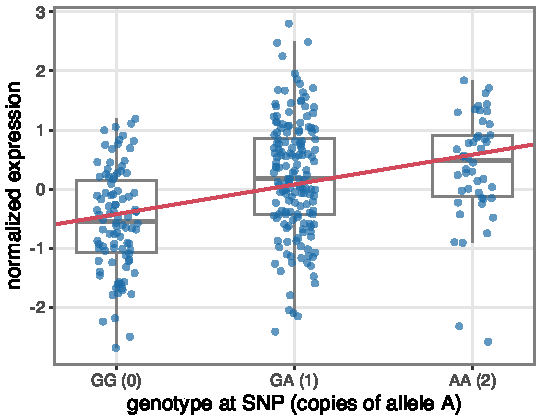
\includegraphics[width=0.5\linewidth]{eqtl_example.pdf}
  \caption{A simulated eQTL in $N=300$ individuals: normalized expression of a gene against genotype at a nearby SNP, with the least-squares fit of~\eqref{eq:eqtl_lm} (red). Each copy of allele A raises expression by about half a standard deviation.}
  \label{fig:eqtl_example}
\end{figure}

When individuals are related, or the cohort has strong population structure, the linear mixed models of Chapter 11 replace~\eqref{eq:eqtl_lm}, with a random effect whose covariance is the genetic relatedness matrix. Simple regression remains the most common choice, and fast matrix implementations test all SNP-gene pairs in a study in minutes~\citep{shabalin2012}.

\subsection{Cis windows and the testing burden}

Which SNPs should be tested for each gene? Empirically, by far the strongest genetic effects on a gene's expression come from variants close to it. The usual practice is to test every SNP within a window, typically 1\,Mb on either side of the transcription start site (TSS). These are \emph{cis}-eQTLs. With roughly one common SNP per kilobase, a 2\,Mb window holds of the order of $M=2000$ SNPs, compared with millions for a GWAS. For chromatin phenotypes such as histone marks or accessibility, genetic effects are even more local, and the window is often only the peak itself plus a few kilobases.

The smaller search space is the second reason eQTL studies work at modest sample size. With Bonferroni correction (below), a GWAS needs a p value below $0.05/(3\times10^6)\approx 1.7\times10^{-8}$, while a single gene's cis window needs $0.05/2000=2.5\times10^{-5}$.

\subsection{Multiple testing at two levels}

Multiple testing in an eQTL study has two levels. For each gene we test $M$ SNPs, and we do this for $P$ genes, typically $P\approx 20{,}000$. The usual strategy is first to compute one p value per gene for the null hypothesis that no SNP in its window affects it, and then to control the false discovery rate across genes.

\paragraph{Within a gene.} Let $p_1,\dots,p_M$ be the p values of the SNPs in the window, and $p_{\min}=\min_m p_m$. Under the null each $p_m$ is uniform on $[0,1]$, so for a threshold $t$ the union bound gives
\begin{equation}
  \Pr(p_{\min}\leq t) = \Pr\Big(\bigcup_{m=1}^M\{p_m\leq t\}\Big) \leq \sum_{m=1}^M\Pr(p_m\leq t) = Mt.
\end{equation}
Choosing $t=0.05/M$ controls the probability of any false positive in the window at 5\%; this is the \emph{Bonferroni correction}, and $\min(1,Mp_{\min})$ is the Bonferroni-adjusted gene-level p value. The bound is close to tight when the tests are independent, since then $\Pr(p_{\min}\leq t)=1-(1-t)^M\approx Mt$ for small $t$. SNPs in a cis window are far from independent: LD makes neighbouring SNPs proxies for each other, so the window contains fewer effectively independent tests than $M$, and Bonferroni is conservative.

\emph{Permutation} gives the exact null distribution of $p_{\min}$ for the window. Permuting the expression values across individuals (equivalently, permuting genotype vectors as whole rows, so that LD between SNPs is preserved) breaks any association between genotype and expression while keeping the LD structure and the distribution of expression. For permutations $b=1,\dots,B$ we recompute $p_{\min}^{(b)}$, and the permutation p value is
\begin{equation}
  p_{\text{perm}} = \frac{1+\sum_{b=1}^B\ind\big[p_{\min}^{(b)}\leq p_{\min}\big]}{B+1}.
\end{equation}
Any statistic can be used in place of $p_{\min}$, for example the maximum $|r|$ or $R^2$. Permutation has to recompute the regressions $B$ times for every gene, which is expensive when small gene-level p values must be resolved; FastQTL~\citep{ongen2016} reduces the cost by fitting a beta distribution to a modest number of permuted $p_{\min}$ values and extrapolating. Covariates complicate permutation, because permuting $y$ also breaks its relation to the covariates; the usual remedy is to regress the covariates out of expression first and permute the residuals. Figure~\ref{fig:permutation_null} compares the permutation null of $p_{\min}$ for a window of independent SNPs and for a window with realistic LD. With LD, the 5\% permutation threshold is several times less stringent than Bonferroni, as if the window contained only a quarter of its SNPs.

\begin{figure}[!htbp]
  \centering
  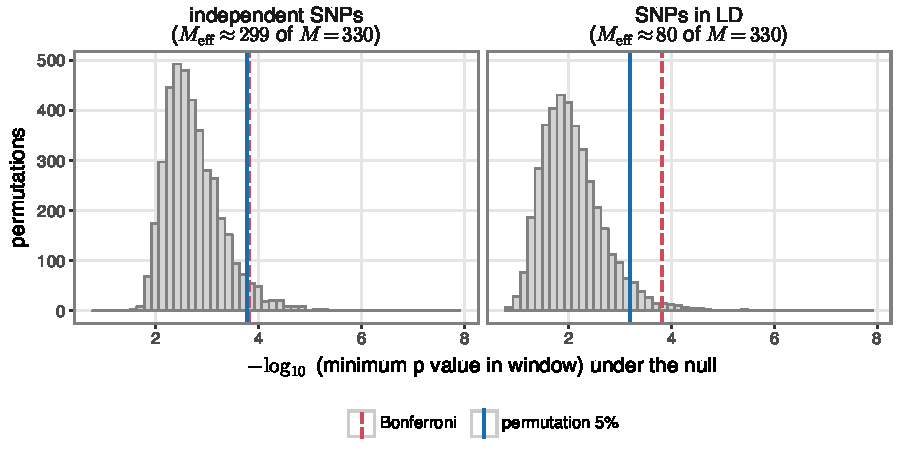
\includegraphics[width=0.85\linewidth]{permutation_null.pdf}
  \caption{Permutation null distribution of the minimum p value across a cis window of $M=330$ SNPs in $N=200$ individuals, from 4000 permutations of a null expression vector. Left, SNPs simulated independently; right, SNPs simulated with block-like LD. The Bonferroni threshold $0.05/M$ (red, dashed) matches the permutation 5\% threshold (blue) for independent SNPs but is conservative with LD. $M_{\text{eff}}=0.05/t_{\text{perm}}$ is the number of independent tests that would give the same threshold.}
  \label{fig:permutation_null}
\end{figure}

\paragraph{Across genes.} Controlling the probability of any false positive across $20{,}000$ genes would be very stringent. Instead we control the \emph{false discovery rate} (FDR), the expected fraction of false positives among the genes we call significant,
\begin{equation}
  \text{FDR} = \E\left[\frac{V}{\max(R,1)}\right],
\end{equation}
where $R$ is the number of genes called eGenes and $V$ the number of those that are null. If we report 5000 eGenes at 10\% FDR, we expect about 500 to be false positives, though we do not know which. The Benjamini-Hochberg (BH) procedure~\citep{benjamini1995} takes the $P$ gene-level p values, sorts them, $p_{(1)}\leq\dots\leq p_{(P)}$, finds the largest $k$ such that
\begin{equation}
  p_{(k)} \leq \frac{k}{P}q,
\end{equation}
and calls the genes with the $k$ smallest p values significant. For independent (or positively dependent) tests this controls the FDR at level $q$. One way to see why: if all $P$ genes were null, about $Pt$ of them would have p values below $t$, so with $k$ genes below $t=p_{(k)}$ the estimated fraction of false discoveries is $Pp_{(k)}/k$, and BH picks the largest set for which this estimate is at most $q$. The $q$-value approach~\citep{storey2003} also estimates the fraction of genes that are null, which gains power when many genes are eGenes. GTEx and most other studies apply the FDR procedure to permutation-based gene-level p values and then, within each eGene, call as eVariants the SNPs whose nominal p values fall below a gene-specific threshold derived from the gene-level cutoff.

%======================================================================
\section{Hidden confounders}
\label{sec:hidden}
%======================================================================

\subsection{Sources of unwanted variation}

Large omics data sets always contain variation that is not the biology we want to study. Some is technical: who prepared the samples, on which day, with which reagent batch, on which sequencing machine. Many eQTL studies use post-mortem tissue, where the \emph{ischaemic time} between death and preservation degrades RNA, and the RNA integrity number (RIN) measures the result. Some is biological but not of interest here: age, sex, environment, recent infections, and in bulk tissue the proportions of different cell types, which vary between people and between pieces of tissue. In GTEx, a study of almost 1000 post-mortem donors and around 50 tissues~\citep{gtex2020}, sample collection variables (ventilator use, ischaemic time, RIN), sequencing batch and library construction are each associated with the main axes of expression variation in many tissues, with $R^2$ up to about 0.3, and estimated cell type proportions are associated to a similar degree.

Such factors affect many genes at once. They do not usually create false eQTLs, because they are not associated with the genotype of a particular SNP, but they add noise to every test and so reduce power. Known factors can be included as covariates in~\eqref{eq:eqtl_lm}. Unknown ones have to be inferred from the expression data.

\subsection{PEER: a factor model for expression}

Chapter 8 introduced factor analysis, $\mY\approx\mX\mW^\top$, and its Bayesian version with an automatic relevance determination (ARD) prior. Because confounders affect many genes, they appear as low-rank structure in the expression matrix, and factor analysis is a natural way to estimate them. PEER (probabilistic estimation of expression residuals)~\citep{stegle2010,stegle2012} combines this with the genetic and known covariate effects in one model (Figure~\ref{fig:peer_model}).

Let $\mY\in\R^{N\times P}$ be the expression matrix of $N$ individuals and $P$ genes (the PEER paper writes the transpose, genes by individuals). The model decomposes it into four parts,
\begin{equation}
  \mY = \underbrace{\mS\mW_S^\top}_{\text{genotype}} + \underbrace{\mF\mW_F^\top}_{\text{known factors}} + \underbrace{\mX\mW^\top}_{\text{hidden factors}} + \mE,
  \label{eq:peer}
\end{equation}
where $\mS\in\{0,1,2\}^{N\times M}$ holds the genotypes of $M$ SNPs with effects $\mW_S\in\R^{P\times M}$; $\mF\in\R^{N\times C}$ holds $C$ measured covariates such as age, sex and batch, with coefficients $\mW_F\in\R^{P\times C}$; $\mX\in\R^{N\times K}$ holds $K$ hidden factors with loadings $\mW\in\R^{P\times K}$; and $\mE\in\R^{N\times P}$ is noise. Element-wise, for gene $p$ and individual $n$,
\begin{equation}
  y_{np}\sim\Normal\Big(\sum_m s_{nm}w^S_{pm}+\sum_c f_{nc}w^F_{pc}+\sum_{k=1}^K x_{nk}w_{pk},\ \tau_p^{-1}\Big),
\end{equation}
with a noise precision $\tau_p$ for each gene, as in factor analysis. The hidden-factor part has the priors of Chapter 8,
\begin{align}
  x_{nk}&\sim\Normal(0,1), & w_{pk}&\sim\Normal(0,\alpha_k^{-1}), & \alpha_k&\sim\Gam(a_\alpha,b_\alpha), & \tau_p&\sim\Gam(a_\tau,b_\tau).
  \label{eq:peer_priors}
\end{align}
The prior precision $\alpha_k$ is shared by all loadings of factor $k$. This is ARD again: if the data do not support factor $k$, $\alpha_k$ grows, the prior variance $1/\alpha_k$ of its loadings shrinks to zero, and the factor is switched off. To see how $\alpha_k$ is set, consider the terms of the log joint density that involve it,
\begin{multline}
  \sum_{p=1}^P\log\Normal(w_{pk}\mid0,\alpha_k^{-1}) + \log\Gam(\alpha_k\mid a_\alpha,b_\alpha) \\ = \frac{P}{2}\log\alpha_k - \frac{\alpha_k}{2}\|\vw_k\|^2 + (a_\alpha-1)\log\alpha_k - b_\alpha\alpha_k + \text{const},
\end{multline}
where $\vw_k\in\R^P$ is column $k$ of $\mW$. Setting the derivative with respect to $\alpha_k$ to zero gives
\begin{equation}
  \hat\alpha_k = \frac{P+2(a_\alpha-1)}{\|\vw_k\|^2+2b_\alpha}\approx\frac{P}{\|\vw_k\|^2},
\end{equation}
the inverse of the mean squared loading. A factor with small loadings gets a large $\alpha_k$, which shrinks its loadings further at the next update, and the iteration drives it to zero. In a variational treatment $\|\vw_k\|^2$ is replaced by its posterior expectation. ARD makes the choice of $K$ less critical: we can set $K$ generously and let the model prune unneeded factors. PEER fits the whole model by mean-field variational Bayes (coordinate ascent variational inference, Chapter 10), which approximates the posterior over $\mX$, $\mW$, $\boldsymbol{\alpha}$ and $\boldsymbol{\tau}$ by a product of independent factors and updates each in turn.

\begin{figure}[!htbp]
  \centering
  \begin{tikzpicture}[>=Stealth, every node/.style={font=\small},
      lat/.style={circle, draw, minimum size=0.85cm, inner sep=0pt},
      obs/.style={circle, draw, double, minimum size=0.85cm, inner sep=0pt},
      plate/.style={draw, rounded corners, inner sep=5pt}]
    \node[obs, fill=green!15] (s) at (0,2.6) {$s_{nm}$};
    \node[lat, fill=green!15] (ws) at (0,0.9) {$w^S_{pm}$};
    \node[obs, fill=blue!12] (f) at (2.4,2.6) {$f_{nc}$};
    \node[lat, fill=blue!12] (wf) at (2.4,0.9) {$w^F_{pc}$};
    \node[lat, fill=red!12] (x) at (4.8,2.6) {$x_{nk}$};
    \node[lat, fill=red!12] (w) at (4.8,0.9) {$w_{pk}$};
    \node[lat, fill=red!12] (al) at (6.4,0.9) {$\alpha_k$};
    \node[obs, fill=gray!20] (y) at (2.4,-1.0) {$y_{np}$};
    \node[lat] (tau) at (4.6,-1.0) {$\tau_p$};
    \draw[->] (s) -- (y); \draw[->] (ws) -- (y);
    \draw[->] (f) -- (y); \draw[->] (wf) -- (y);
    \draw[->] (x) -- (y); \draw[->] (w) -- (y);
    \draw[->] (al) -- (w); \draw[->] (tau) -- (y);
    \node[plate, fit=(s)(ws), label={[green!40!black]above:SNPs $m$}] {};
    \node[plate, fit=(f)(wf), label={[blue!60!black]above:covariates $c$}] {};
    \node[plate, fit=(x)(w)(al), label={[red!60!black]above:factors $k$}] {};
    \node[plate, fit=(ws)(wf)(w)(y)(tau), inner sep=12pt, label={[gray]below:genes $p$}] {};
  \end{tikzpicture}
  \caption{Graphical model of PEER, after \citet{stegle2010}. Double circles are observed; plates denote replication over SNPs, covariates, hidden factors and genes (the plate over individuals $n$, which contains $s_{nm}$, $f_{nc}$, $x_{nk}$ and $y_{np}$, is omitted for clarity). The ARD precision $\alpha_k$ controls whether hidden factor $k$ is used.}
  \label{fig:peer_model}
\end{figure}

\subsection{PEER in practice}

Fitting all four components of~\eqref{eq:peer} jointly is slow and difficult. In practice the genotype term is left out of the factor model: the known covariates and hidden factors are fitted first, as a pre-processing step, and the eQTL tests are then run with the simple regression~\eqref{eq:eqtl_lm}, either on the residuals or with the inferred factors $\hat\mX$ included as covariates. GTEx chose the number of PEER factors by sample size, using more factors for tissues with more samples. Simpler alternatives work about as well: taking the top principal components of the expression matrix as covariates, as in Chapter 8, matches or outperforms PEER in benchmarks~\citep{zhou2022pca}.

Removing hidden factors greatly increases the number of eQTLs found. In GTEx tissues, the number of eGenes detected at 5\% FDR roughly doubles as the number of PEER factors included as covariates increases from 0 to 60, with diminishing returns beyond that~\citep{fan2020}. Figure~\ref{fig:hidden_factors} shows the same effect on simulated data, which also shows ARD at work. The simulated expression of $P=2000$ genes in $N=200$ individuals has $K=10$ hidden factors and one cis SNP per gene, 30\% of which have a genetic effect. An ARD factor analysis model started with 30 factors keeps exactly 10 (Figure~\ref{fig:hidden_factors}a), and regressing out these factors finds as many eGenes as regressing out the true factors, three times as many as with no correction (Figure~\ref{fig:hidden_factors}b). Regressing out expression principal components improves power up to the true number of factors. Beyond that, extra components capture noise; removing them costs degrees of freedom and removes some genetic signal by chance, so power declines. In real data, with many confounders of decreasing strength, the curve usually rises and then plateaus instead.

\begin{figure}[!htbp]
  \centering
  \begin{subfigure}[b]{0.48\linewidth}
    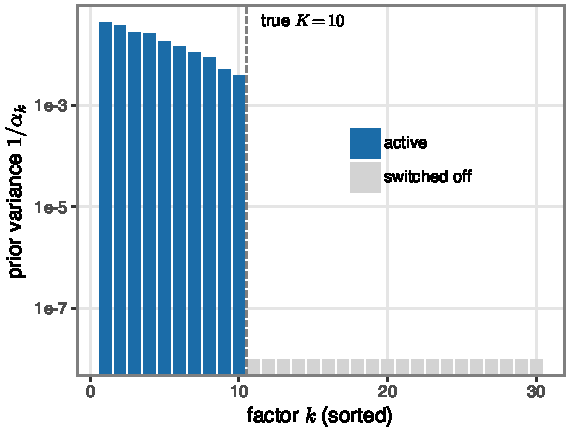
\includegraphics[width=\linewidth]{ard_factors.pdf}
    \caption{}
  \end{subfigure}\hfill
  \begin{subfigure}[b]{0.48\linewidth}
    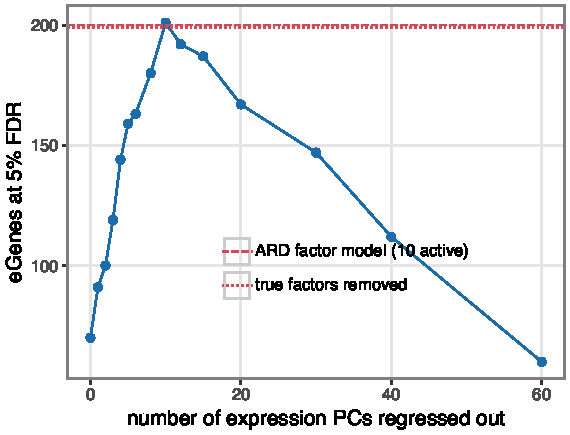
\includegraphics[width=\linewidth]{hidden_factors_power.pdf}
    \caption{}
  \end{subfigure}
  \caption{Removing hidden confounders from simulated expression ($N=200$ individuals, $P=2000$ genes, $K=10$ hidden factors). (a) Prior variances $1/\alpha_k$ of the factors of an ARD factor analysis model fitted with 30 factors (the switched-off factors are at the numerical floor $10^{-8}$). (b) eGenes detected at 5\% FDR after regressing out increasing numbers of expression principal components (blue), the 10 active ARD factors (dotted) or the true factors (dashed); the two horizontal lines coincide. The simulation has 617 true eGenes.}
  \label{fig:hidden_factors}
\end{figure}

There are two caveats. First, the factors should capture confounders, not the genetic signal itself. Cis effects are specific to one gene each and are not low-rank, so they survive. A trans-acting variant that changes the expression of many genes, for example through a transcription factor, does produce low-rank structure, and regressing out factors can remove it; hidden-factor correction is therefore risky for trans-eQTL analysis. Second, factors can capture interesting biology, such as cell type composition or an immune response. Removing them helps in finding eQTLs that act in all conditions, at the cost of hiding those whose effect depends on the condition (Section~\ref{sec:interaction}).

%======================================================================
\section{Cis and trans effects}
%======================================================================

A cis-eQTL acts on the copy of the gene on the same chromosome, typically through a promoter or enhancer variant that changes transcription factor binding (Figure~\ref{fig:cis_trans}, top). Cis-eQTLs are the classical eQTL: they are robust, replicate well between studies, and can be found with as few as 70 individuals. A \emph{trans}-eQTL acts at a distance, usually on another chromosome. A typical mechanism is a variant that changes the expression or the protein sequence of a transcription factor, which then changes the expression of the factor's targets throughout the genome (Figure~\ref{fig:cis_trans}, bottom). Trans effects are biologically interesting, since they reveal regulatory networks, but they are hard to find and to replicate. Each effect is small, and without a window to restrict the search we are back to testing millions of SNPs per gene, with a testing burden of millions of SNPs times $20{,}000$ genes. Reliable trans-eQTL mapping needs thousands of individuals, and false positives from technical artefacts, such as reads from one gene mis-mapped to a paralogous gene elsewhere in the genome, are a constant worry.

The cis-trans distinction is about mechanism, not distance alone: a cis effect is one that acts only on the allele on the same DNA molecule. This is what allele-specific expression measures, as we see next. In practice, eQTL studies use physical distance as a proxy and call any SNP within 1\,Mb of a gene cis.

\begin{figure}[!htbp]
  \centering
  \begin{tikzpicture}[>=Stealth, every node/.style={font=\small}, tf/.style={regular polygon, regular polygon sides=5, draw, fill=violet!20, minimum size=0.55cm, inner sep=0pt}]
    % cis
    \node[anchor=west] at (-0.3,0.9) {\textbf{cis}};
    \draw[thick, blue!60!black] (0,0) -- (8,0);
    \draw[fill=blue!20] (4,-0.18) rectangle (6.5,0.18);
    \node at (5.25,0) {\footnotesize gene};
    \draw[->, thick, blue!60!black] (4,0.18) -- (4,0.45) -- (4.6,0.45);
    \node[tf] at (2,0.42) {};
    \node[fill=white, inner sep=1pt] at (2,0) {\footnotesize G};
    \draw[->, dashed] (2.3,0.6) to[out=30, in=150] node[above] {\footnotesize same chromosome} (4.1,0.7);
    \draw[thick, magenta!70!black] (0,-1.0) -- (8,-1.0);
    \draw[fill=magenta!15] (4,-1.18) rectangle (6.5,-0.82);
    \node at (5.25,-1.0) {\footnotesize gene};
    \draw[->, magenta!70!black] (4,-0.82) -- (4,-0.65) -- (4.3,-0.65);
    \node[fill=white, inner sep=1pt] at (2,-1.0) {\footnotesize A};
    \node[tf] at (1.3,-0.55) {};
    \draw[decorate, decoration={snake, amplitude=1pt, segment length=4pt}, red!70!black] (6.8,0.15) -- (7.8,0.15);
    \draw[decorate, decoration={snake, amplitude=1pt, segment length=4pt}, red!70!black] (6.8,0.40) -- (7.8,0.40);
    \draw[decorate, decoration={snake, amplitude=1pt, segment length=4pt}, red!70!black] (6.8,-0.75) -- (7.8,-0.75);
    \node[right, align=left] at (8.2,-0.4) {\footnotesize two haplotypes\\\footnotesize of one person};
    % trans
    \begin{scope}[yshift=-3.0cm]
      \node[anchor=west] at (-0.3,0.9) {\textbf{trans}};
      \draw[thick] (0,0) -- (3.4,0);
      \draw[fill=violet!15] (1.0,-0.18) rectangle (2.6,0.18);
      \node at (1.8,0) {\footnotesize TF gene};
      \node[fill=white, inner sep=1pt] at (0.5,0) {\footnotesize G/A};
      \node[below] at (1.7,-0.25) {\footnotesize chromosome 1};
      \draw[thick] (4.6,0) -- (8,0);
      \draw[fill=blue!20] (6.2,-0.18) rectangle (7.8,0.18);
      \node at (7.0,0) {\footnotesize target};
      \node[below] at (6.3,-0.25) {\footnotesize chromosome 7};
      \node[tf] (t) at (5.4,0.42) {};
      \draw[->, dashed] (2.6,0.3) to[out=40, in=150] node[above] {\footnotesize TF protein} (t.north west);
    \end{scope}
  \end{tikzpicture}
  \caption{Cis and trans effects. Top: a cis-regulatory variant changes binding of a transcription factor (pentagon) near a gene and so changes expression only of the copy of the gene on the same chromosome, giving more RNA from the G haplotype. Bottom: a trans effect, in which a variant in or near a transcription factor (TF) gene changes the TF's level or activity, which changes expression of its target genes elsewhere in the genome, on both of their copies.}
  \label{fig:cis_trans}
\end{figure}

%======================================================================
\section{Linkage disequilibrium and the causal variant}
%======================================================================

An eQTL association has the same problem as a GWAS association: LD. Figure~\ref{fig:ld_locus} shows a simulated cis window in which one SNP affects expression. Many SNPs in high LD with it are almost as significant, SNPs in moderate LD are moderately significant, and with a little noise the most significant SNP need not be the causal one. SNPs in LD act as proxies, or \emph{tag SNPs}, for the causal variant. The ease of finding an associated locus and the difficulty of finding the variant within it are two sides of the same coin. Fine-mapping methods (Chapter 11), such as SuSiE~\citep{wang2020susie}, compute for each SNP the posterior probability that it is causal and report credible sets that contain a causal variant with high probability, allowing for several causal variants per gene. Functional annotations can sharpen the posterior (Section~\ref{sec:annotations}). The definitive test is experimental: editing the variant with CRISPR and measuring expression, which has been done for the lead variants of some eQTLs.

\begin{figure}[!htbp]
  \centering
  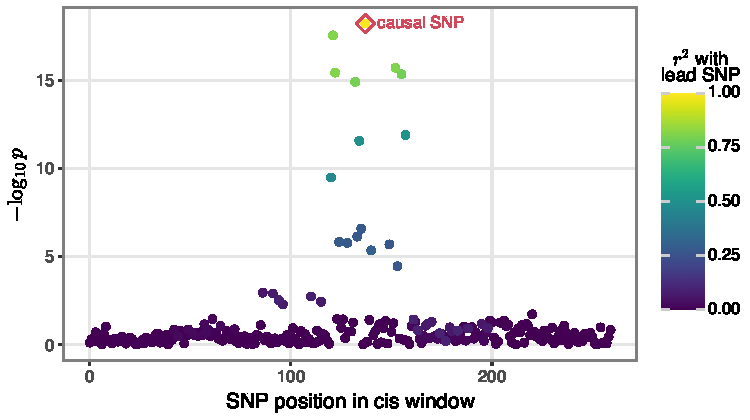
\includegraphics[width=0.7\linewidth]{ld_locus.pdf}
  \caption{A simulated cis-eQTL with one causal SNP (diamond) among 260 SNPs with block-like LD, in $N=500$ individuals. Each point is a SNP, coloured by its LD ($r^2$) with the most significant (lead) SNP. SNPs in high LD with the causal variant are nearly as significant as the causal variant.}
  \label{fig:ld_locus}
\end{figure}

%======================================================================
\section{Allele-specific expression}
\label{sec:ase}
%======================================================================

\subsection{Two views of the same cis effect}

A cis-eQTL can be seen in two ways (Figure~\ref{fig:ase}). Across individuals, those with more copies of the high-expression allele have higher total expression of the gene. Within a single individual who is heterozygous at the regulatory variant, the copy of the gene on the haplotype with the high-expression allele produces more RNA than the copy on the other haplotype. (A \emph{haplotype} is the sequence of one of the two copies of a chromosome, one inherited from each parent.) To see the within-individual difference we need a way to tell the RNA from the two copies apart. If the individual is also heterozygous at a SNP in the transcribed sequence, for example a coding or UTR SNP with alleles T and C, RNA-seq reads that cover it carry one allele or the other, and counting them measures \emph{allele-specific expression} (ASE). An imbalance away from 50:50 indicates a cis-regulatory difference between the two haplotypes.

\begin{figure}[!htbp]
  \centering
  \begin{tikzpicture}[>=Stealth, every node/.style={font=\small}, tf/.style={regular polygon, regular polygon sides=5, draw, fill=violet!20, minimum size=0.6cm, inner sep=0pt}]
    \draw[thick, blue!60!black] (0,0) -- (7.5,0);
    \draw[fill=blue!15] (3.2,-0.22) rectangle (6.4,0.22);
    \fill[green!30] (5.0,-0.2) rectangle (5.35,0.2); \node at (5.17,0) {T};
    \draw[->, very thick, blue!60!black] (3.2,0.22) -- (3.2,0.6) -- (4.0,0.6);
    \node[tf] at (1.8,0.33) {};
    \node[fill=white, inner sep=1pt] at (1.8,-0.05) {\footnotesize G};
    \draw[thick, blue!60!black] (0,-1.2) -- (7.5,-1.2);
    \draw[fill=blue!15] (3.2,-1.42) rectangle (6.4,-0.98);
    \fill[violet!30] (5.0,-1.4) rectangle (5.35,-1.0); \node at (5.17,-1.2) {C};
    \draw[->, blue!60!black] (3.2,-0.98) -- (3.2,-0.75) -- (3.6,-0.75);
    \node[fill=white, inner sep=1pt] at (1.8,-1.2) {\footnotesize A};
    \node[tf] at (1.0,-0.65) {};
    \node[above] at (1.8,0.75) {regulatory variant};
    \node[above] at (5.17,0.55) {exonic SNP};
    % reads
    \foreach \y/\a in {-2.0/T,-2.3/T,-2.6/T,-2.9/T} {
      \draw[green!50!black, thick] (4.3,\y) -- (4.95,\y); \draw[green!50!black, thick] (5.4,\y) -- (6.1,\y);
      \node at (5.17,\y) {\footnotesize \a};}
    \foreach \y/\a in {-3.2/C,-3.5/C} {
      \draw[violet!70!black, thick] (4.3,\y) -- (4.95,\y); \draw[violet!70!black, thick] (5.4,\y) -- (6.1,\y);
      \node at (5.17,\y) {\footnotesize \a};}
    \node[right, align=left] at (6.3,-2.75) {RNA-seq reads:\\4 T, 2 C};
  \end{tikzpicture}
  \caption{Allele-specific expression. In an individual heterozygous at a regulatory variant, a transcription factor (pentagon) binds the G allele but not the A allele, so the copy of the gene on the G haplotype is expressed more. If the individual is also heterozygous at a SNP in the transcript (T/C), RNA-seq reads covering it can be assigned to a haplotype, and the read counts show the imbalance.}
  \label{fig:ase}
\end{figure}

ASE requires an individual to be heterozygous at a transcribed SNP, and, to connect the imbalance to a candidate regulatory variant, the phase of the two SNPs: which allele of the regulatory variant lies on the same haplotype as which allele of the exonic SNP. Phase is estimated statistically from population genotype data or read directly from long reads. The heterozygous exonic SNP is only a marker. It is usually not the cause of the imbalance, which is due to some other variant in cis. The same idea applies to other sequencing assays. In ChIP-seq or ATAC-seq, reads overlapping a heterozygous SNP in a binding site or accessible region measure allele-specific binding or accessibility, and there the SNP being counted is often itself the cause, since a variant inside a binding site can directly change binding.

\subsection{Counting alleles: binomial and beta-binomial models}

Consider one individual and one heterozygous exonic SNP. Let $d$ be the number of reads covering the SNP that carry either allele, $y\leq d$ the number carrying the reference allele, and $\pi$ the expected fraction of reads from the reference haplotype. If reads were independent draws,
\begin{equation}
  y\mid d,\pi \sim \Bin(d,\pi), \qquad \Pr(y\mid d,\pi) = \binom{d}{y}\pi^y(1-\pi)^{d-y},
\end{equation}
and testing for allelic imbalance means testing $H_0:\pi=1/2$. Reads are not independent draws, however. Library preparation amplifies the cDNA by PCR, so several reads can come from one original molecule; mapping and capture efficiencies vary from site to site; and the true imbalance varies between individuals and cells. All of these make the counts more variable than the binomial allows, and a binomial test applied to such data reports far too many significant imbalances.

The \emph{beta-binomial} distribution adds this extra variation by treating $\pi$ as random. Let $\pi\sim\BetaDist(a,b)$ with $a,b>0$ and density
\begin{equation}
  p(\pi\mid a,b) = \frac{\pi^{a-1}(1-\pi)^{b-1}}{\BetaFn(a,b)}, \qquad \BetaFn(a,b)=\int_0^1 u^{a-1}(1-u)^{b-1}du = \frac{\Gamma(a)\Gamma(b)}{\Gamma(a+b)}.
\end{equation}
The beta is the conjugate prior of the binomial (the density has the same form $\pi^{\cdot}(1-\pi)^{\cdot}$ as the likelihood) and is the two-category case of the Dirichlet distribution used for isoform proportions in Chapter 10. Its mean and variance are
\begin{equation}
  \E[\pi] = \frac{a}{a+b}=:\mu, \qquad \Var(\pi) = \frac{ab}{(a+b)^2(a+b+1)} = \frac{\mu(1-\mu)}{c+1},
\end{equation}
where $c=a+b$ is the \emph{concentration}. The ratio of $a$ to $b$ sets the mean, and the concentration sets how tightly $\pi$ is distributed around it. Integrating $\pi$ out gives the beta-binomial,
\begin{align}
  \Pr(y\mid d,a,b) &= \int_0^1\binom{d}{y}\pi^y(1-\pi)^{d-y}\,\frac{\pi^{a-1}(1-\pi)^{b-1}}{\BetaFn(a,b)}\,d\pi \nonumber\\
  &= \binom{d}{y}\frac{1}{\BetaFn(a,b)}\int_0^1\pi^{y+a-1}(1-\pi)^{d-y+b-1}\,d\pi
  = \binom{d}{y}\frac{\BetaFn(y+a,\,d-y+b)}{\BetaFn(a,b)}.
  \label{eq:betabinom}
\end{align}
We write $\BetaBin(y\mid d,\mu,c)$ for this distribution parameterized by its mean fraction $\mu=a/c$ and concentration $c$, so $a=\mu c$ and $b=(1-\mu)c$. The moments follow from the laws of total expectation and variance. The mean is $\E[y]=\E[\E[y\mid\pi]]=d\E[\pi]=d\mu$. For the variance,
\begin{align}
  \Var(y) &= \E[\Var(y\mid\pi)] + \Var(\E[y\mid\pi]) = d\,\E[\pi(1-\pi)] + d^2\Var(\pi) \nonumber\\
  &= d\big(\mu(1-\mu)-\Var(\pi)\big) + d^2\Var(\pi) = d\mu(1-\mu) + d(d-1)\Var(\pi) \nonumber\\
  &= d\mu(1-\mu)\left[1+\frac{d-1}{c+1}\right],
\end{align}
using $\E[\pi(1-\pi)]=\E[\pi]-\E[\pi^2]=\mu-\Var(\pi)-\mu^2$. The first factor is the binomial variance, and the bracket is the overdispersion factor. As $c\to\infty$ it tends to one and the beta-binomial becomes the binomial; small $c$ means noisy allelic counts. Figure~\ref{fig:count_models}a compares a binomial and a beta-binomial with the same mean: the beta-binomial with $c=17$ and $d=30$ has a variance $2.6$ times larger.

\subsection{Counting molecules: Poisson and negative binomial models}

The total read count for a gene in an individual is a count without a fixed number of trials. The basic model is the Poisson, $y\sim\Pois(\lambda)$ with $\Pr(y\mid\lambda)=\lambda^ye^{-\lambda}/y!$, the limit of a binomial with many trials, each with small success probability. Like the binomial it has one parameter: $\E[y]=\Var(y)=\lambda$, so fixing the mean fixes the variance. RNA-seq counts are much more variable between biological replicates than this, for the same reasons as allelic counts and because true expression varies between individuals.

The fix follows the same recipe. Let the rate be random, $\lambda\sim\Gam(\phi,r)$ with shape $\phi$ and rate $r$, density $r^\phi\lambda^{\phi-1}e^{-r\lambda}/\Gamma(\phi)$, mean $\phi/r$ and variance $\phi/r^2$. The gamma is conjugate to the Poisson, and integrating out $\lambda$ gives
\begin{align}
  \Pr(y\mid\phi,r) &= \int_0^\infty \frac{\lambda^ye^{-\lambda}}{y!}\,\frac{r^\phi\lambda^{\phi-1}e^{-r\lambda}}{\Gamma(\phi)}\,d\lambda
  = \frac{r^\phi}{y!\,\Gamma(\phi)}\int_0^\infty\lambda^{y+\phi-1}e^{-(r+1)\lambda}\,d\lambda \nonumber\\
  &= \frac{r^\phi}{y!\,\Gamma(\phi)}\,\frac{\Gamma(y+\phi)}{(r+1)^{y+\phi}}
  = \frac{\Gamma(y+\phi)}{\Gamma(\phi)\,y!}\left(\frac{r}{r+1}\right)^\phi\left(\frac{1}{r+1}\right)^y,
\end{align}
the \emph{negative binomial} distribution, better described as the gamma-Poisson. (Its name comes from another derivation, as the number of failures before the $\phi$-th success in a sequence of coin flips with success probability $r/(r+1)$.) The mean is $m=\E[y]=\E[\lambda]=\phi/r$, and by the law of total variance
\begin{equation}
  \Var(y) = \E[\Var(y\mid\lambda)]+\Var(\E[y\mid\lambda]) = \E[\lambda]+\Var(\lambda) = \frac{\phi}{r}+\frac{\phi}{r^2} = m + \frac{m^2}{\phi}.
\end{equation}
We write $\NB(y\mid m,\phi)$ for the distribution with mean $m$ and shape $\phi$, so $r=\phi/m$. The variance always exceeds the Poisson variance $m$, by an amount controlled by the shape, which plays the role of a concentration: as $\phi\to\infty$ we recover the Poisson. $1/\phi$ is called the dispersion, and the same model underlies standard differential expression tools. Figure~\ref{fig:count_models}b compares a Poisson and a negative binomial with mean 30; with $\phi=8$ the variance is $30+900/8=142.5$ rather than 30.

\begin{figure}[!htbp]
  \centering
  \begin{subfigure}[b]{0.48\linewidth}
    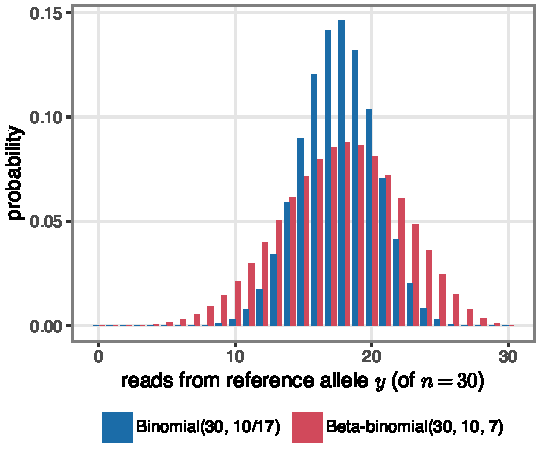
\includegraphics[width=\linewidth]{betabinom.pdf}
    \caption{}
  \end{subfigure}\hfill
  \begin{subfigure}[b]{0.48\linewidth}
    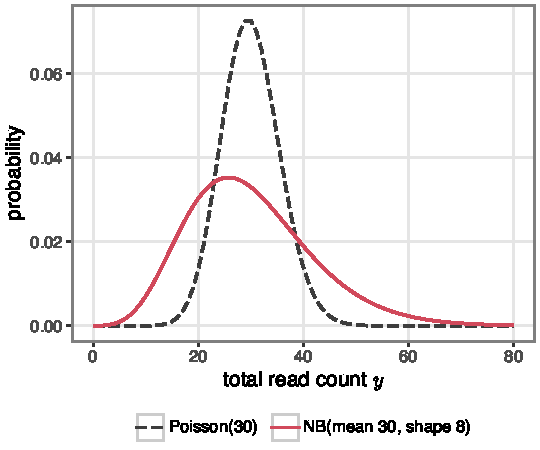
\includegraphics[width=\linewidth]{negbin.pdf}
    \caption{}
  \end{subfigure}
  \caption{Overdispersed count models. (a) Binomial with $d=30$ trials and $\pi=10/17$ and beta-binomial with $d=30$, $a=10$, $b=7$; both have mean 17.6, but the variances are 7.3 and 19.0. (b) Poisson with mean 30 and negative binomial with mean 30 and shape $\phi=8$.}
  \label{fig:count_models}
\end{figure}

\subsection{Combining total and allele-specific counts}

The combined haplotype test (CHT)~\citep{mcvicker2013}, implemented in WASP~\citep{vandegeijn2015}, uses both the between-individual signal in total counts and the within-individual signal in allelic counts to test a candidate cis-regulatory SNP. We describe a simplified version. Let $\theta_R$ and $\theta_A$ be the expression of one copy of the gene on a haplotype carrying the reference and the alternative allele of the test SNP. The expected allelic fraction in a heterozygote is the \emph{allelic imbalance}
\begin{equation}
  \pi = \frac{\theta_R}{\theta_R+\theta_A},
\end{equation}
and the expected total expression of individual $n$ depends on their genotype at the test SNP,
\begin{equation}
  \lambda_n = T_n\times\begin{cases} 2\theta_R & \text{if $n$ is homozygous reference},\\ \theta_R+\theta_A & \text{if $n$ is heterozygous},\\ 2\theta_A & \text{if $n$ is homozygous alternative}, \end{cases}
\end{equation}
where $T_n$ is a scaling factor for how deeply individual $n$ was sequenced. This is the additive model of~\eqref{eq:eqtl_lm} on the count scale. For individual $n$, let $y^t_n$ be the total read count of the gene and $y^a_n$ the number of reads from the haplotype carrying the reference allele of the test SNP, out of $d_n$ reads covering heterozygous exonic SNPs (using the phase to assign reads to haplotypes). The likelihood is
\begin{equation}
  L(\theta_R,\theta_A) = \prod_{n=1}^N \NB\big(y^t_n\mid\lambda_n,\phi\big)\;\prod_{n:\,\text{het}}\BetaBin\big(y^a_n\mid d_n,\pi,c\big)\;\prod_{n:\,\text{hom}}\BetaBin\big(y^a_n\mid d_n,\tfrac12,c\big),
  \label{eq:cht}
\end{equation}
with shape $\phi$ and concentration $c$ estimated across genes. Individuals who are homozygous at the test SNP have the same regulatory allele on both haplotypes, so their allelic counts are expected to be balanced; their term does not depend on $\theta$, but it would show imbalance, and so evidence against this SNP, if the true causal variant were a different one. The test of $H_0:\theta_R=\theta_A$ is a \emph{likelihood ratio test}: maximize~\eqref{eq:cht} with $\theta_R$ and $\theta_A$ free and with $\theta_R=\theta_A$, and compare
\begin{equation}
  \Lambda = 2\left[\log L(\hat\theta_R,\hat\theta_A) - \log L(\hat\theta_0,\hat\theta_0)\right]
\end{equation}
with a $\chi^2_1$ distribution, which by Wilks' theorem is its distribution under the null for large samples. The full CHT also models genotyping errors and estimates the dispersions per individual. WASP also corrects \emph{reference mapping bias}: reads carrying the reference allele align to the reference genome slightly more easily than reads carrying the alternative allele, which mimics allelic imbalance. WASP flips the allele in each read that overlaps a SNP, remaps it, and discards reads that do not map to the same place. RASQUAL~\citep{kumasaka2016} is a related model that combines the two signals and also handles uncertainty in phasing.

\subsection{Calibration and power}

Results of genome-wide tests are summarized by \emph{quantile-quantile (QQ) plots} (Figure~\ref{fig:ase_qq}). If the test is calibrated, its p values are uniform on $[0,1]$ under the null. We sort the $J$ observed p values and plot $-\log_{10}$ of each against $-\log_{10}$ of the corresponding uniform quantile, $(i-0.5)/J$ for the $i$-th smallest. If there is no signal, the points lie on the diagonal. True associations bend the curve upward at the right, while a curve that leaves the diagonal from the start indicates a miscalibrated test or confounding.

Figure~\ref{fig:ase_qq} shows both effects on simulated data with 20 individuals and 2000 SNP-gene pairs, 20\% with a true cis effect, using overdispersed counts ($\phi=10$, $c=30$). On null genes (panel a), a binomial test of allelic imbalance is badly inflated: 14\% of null tests have $p<0.05$. The beta-binomial test with the correct concentration is calibrated (5.4\%). On all genes (panel b), the combined test of~\eqref{eq:cht} finds more than twice as many associations at 5\% FDR as a linear regression on log total counts (232 versus 95 of 407 true effects). \citet{vandegeijn2015} found the same in real data: on H3K27ac ChIP-seq from only 10 lymphoblastoid cell lines, where the linear model found almost nothing, the combined test found many histone QTLs, and it also found substantially more eQTLs in 70 lymphoblastoid cell lines.

\begin{figure}[!htbp]
  \centering
  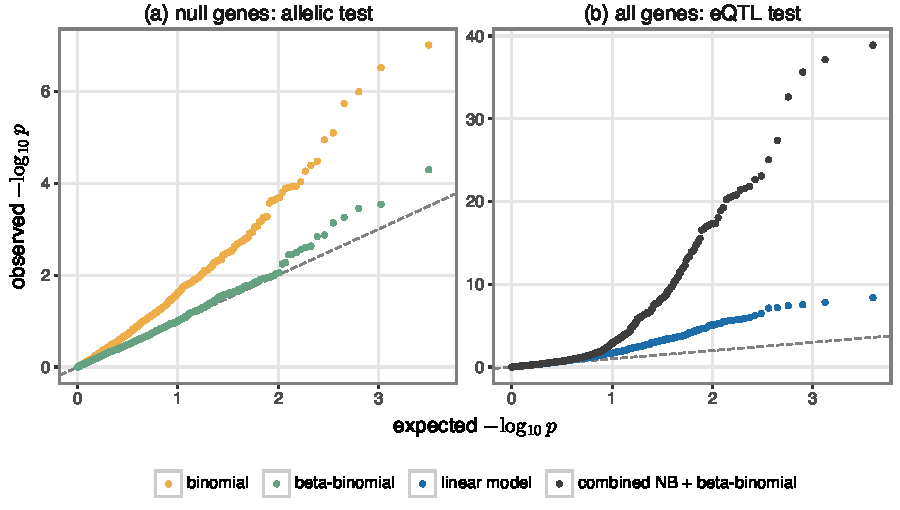
\includegraphics[width=0.9\linewidth]{ase_qq.pdf}
  \caption{QQ plots of simulated allele-specific tests ($N=20$ individuals, 2000 SNP-gene pairs, 20\% with a cis effect, overdispersed counts). (a) Tests of allelic imbalance among heterozygotes on null genes: the binomial test is inflated, the beta-binomial test is calibrated. (b) eQTL tests on all genes: linear regression of log total counts on genotype, and the combined likelihood ratio test of total (negative binomial) and allelic (beta-binomial) counts. Dashed line, $y=x$.}
  \label{fig:ase_qq}
\end{figure}

Why is the within-individual comparison so powerful? The two haplotypes of an individual are in the same cells, in the same tissue, exposed to the same environment and processed in the same experiment. Comparing them is a built-in control: almost all of the technical and environmental variation that differs between people cancels, leaving the effect of the sequence difference. This gives some insight into regulatory variation even with very small samples, where between-individual eQTL mapping fails. It also separates cis from trans effects, since a trans effect, acting through a diffusible factor, affects both copies of a gene equally. The limitations are that a gene must carry a heterozygous transcribed SNP with enough reads in enough individuals, and that the extra machinery (phasing, mapping bias correction, overdispersion) makes the analysis slower and more involved.

%======================================================================
\section{Lessons from tissue atlases}
%======================================================================

\subsection{eQTLs and sQTLs across tissues}

The Genotype-Tissue Expression (GTEx) project collected RNA-seq from around 50 tissues of almost 1000 post-mortem donors, with whole-genome sequencing of each donor~\citep{gtex2017,gtex2020}. The number of samples per tissue ranges from under 100 to around 700, because some tissues are much harder to collect than others. Figure~\ref{fig:gtex_egenes} shows the fraction of tested genes with a significant cis-eQTL or cis-sQTL in each tissue. Discovery grows steadily with sample size and has not saturated, and eQTLs are easier to detect than sQTLs. Across tissues, 95\% of protein-coding genes have at least one cis-eQTL and 79\% at least one cis-sQTL. With larger samples, conditional analysis (adding the lead variant as a covariate and searching again) finds a second, third or further independent eVariant for an increasing fraction of genes, so the one-causal-variant-per-gene picture is a consequence of limited power rather than biology. Trans-eQTLs were found for only on the order of a hundred genes, consistent with their small effects.

\begin{figure}[!htbp]
  \centering
  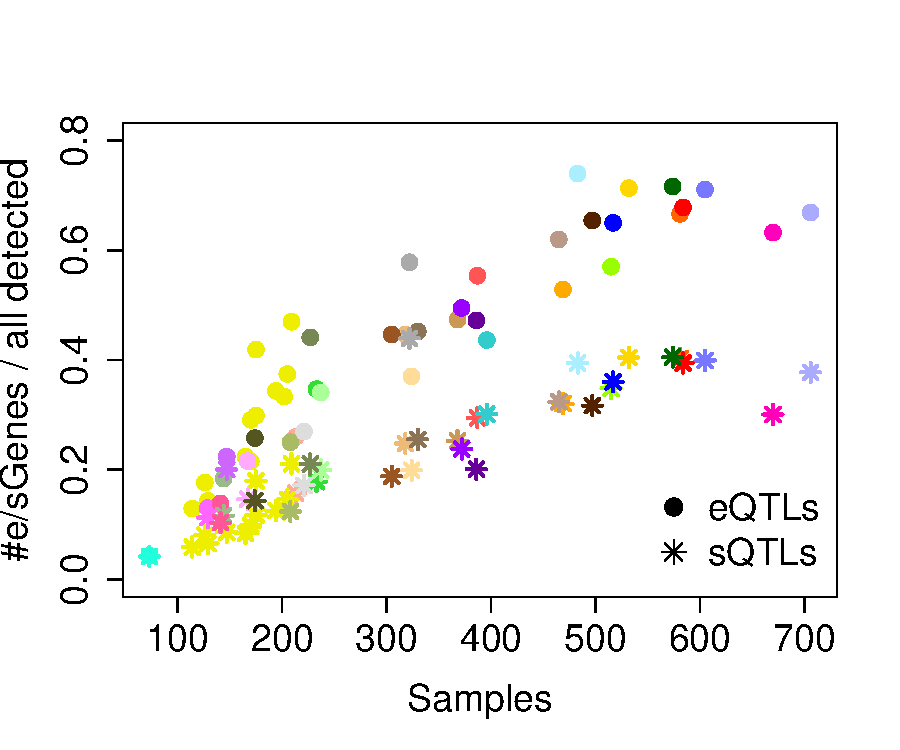
\includegraphics[width=0.5\linewidth]{slides/gtex_egenes.pdf}
  \caption{Fraction of tested genes with a cis-eQTL (eGenes, dots) or cis-sQTL (sGenes, stars) at 5\% FDR, against the number of samples, for each GTEx tissue (colours). From the GTEx Consortium~\citep{gtex2020}.}
  \label{fig:gtex_egenes}
\end{figure}

\subsection{Sharing of eQTLs across tissues}

How much of the genetic regulation of expression is shared between tissues? The naive approach maps eQTLs separately in each tissue and counts how often an eQTL significant in one is also significant in another. This confuses the absence of evidence with evidence of absence. Tissues differ in sample size and therefore in power, so an eQTL can be significant in one tissue and not another just because the second has fewer samples. Figure~\ref{fig:sharing_naive} shows this for simulated eQTLs whose true effects are identical in two tissues with 500 and 150 samples: of the eQTLs significant in at least one tissue, 77\% are significant only in the larger one and would be called tissue-specific. Early studies made exactly this mistake and concluded that eQTLs are mostly tissue-specific. The general lesson is that comparing ``significant in condition 1'' with ``significant in condition 2'' is not a test of whether the effect differs; that requires a model of the effects in both conditions together.

\begin{figure}[!htbp]
  \centering
  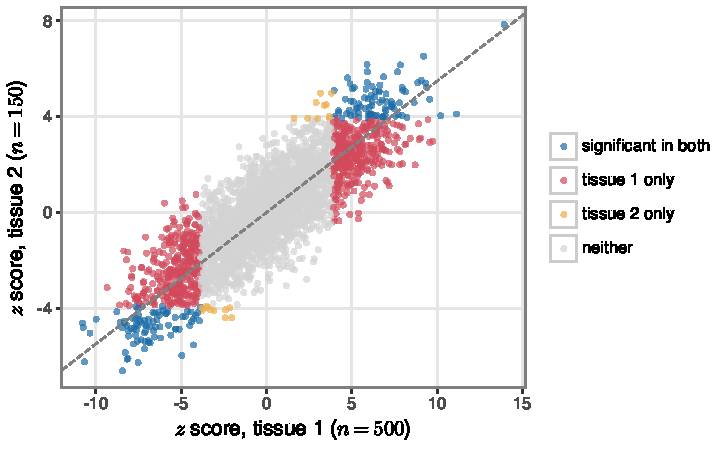
\includegraphics[width=0.62\linewidth]{sharing_naive.pdf}
  \caption{The ``significant here, not there'' fallacy. Simulated $z$ scores for 3000 eQTLs with the same true effect in two tissues, measured in 500 and 150 individuals. Points are coloured by whether they pass $p<10^{-4}$ in both, one or neither tissue. Most eQTLs significant in the larger tissue are not significant in the smaller one, although none is tissue-specific. Dashed line, the expected ratio $\sqrt{150/500}$ of the $z$ scores.}
  \label{fig:sharing_naive}
\end{figure}

Multivariate adaptive shrinkage (mash)~\citep{urbut2019} models the effects jointly from summary statistics. For SNP-gene pair $j$ and tissue $r=1,\dots,R$, let $b_{jr}$ be the true effect, $\hat b_{jr}$ its estimate (from~\eqref{eq:eqtl_lm} or another test) and $s_{jr}$ the standard error of $\hat b_{jr}$. Collect them into vectors $\vbb_j,\vbhat_j\in\R^R$ and the diagonal matrix $\mS_j=\diag(s_{j1}^2,\dots,s_{jR}^2)$. The likelihood treats the estimates as unbiased and normally distributed,
\begin{equation}
  \vbhat_j\mid\vbb_j \sim \Normal(\vbb_j,\mS_j),
\end{equation}
which can be extended to correlated errors when tissues share donors. The prior on the vector of true effects is a mixture of zero-mean multivariate normals,
\begin{equation}
  \vbb_j \sim \sum_{k=1}^K\sum_{l=1}^L \pi_{kl}\,\Normal(\vzero,\omega_l\mU_k), \qquad \sum_{k,l}\pi_{kl}=1,
  \label{eq:mash_prior}
\end{equation}
where each $\mU_k\in\R^{R\times R}$ is a candidate covariance matrix describing a pattern of sharing across tissues, $\omega_l>0$ is one of $L$ scaling factors on a fixed grid, and $\pi_{kl}\geq0$ are mixture weights. The $\mU_k$ include \emph{canonical} matrices (the identity, for independent effects in each tissue; a matrix of ones, for an identical effect in all tissues; and $R$ matrices with a single non-zero diagonal entry, for an effect in only one tissue) and \emph{data-driven} matrices estimated from the strongest associations, for example by PCA or sparse factor analysis of their $z$ scores. Because the prior and likelihood are Gaussian, $\vbb_j$ can be integrated out within each component,
\begin{equation}
  \vbhat_j \sim \sum_{k,l}\pi_{kl}\,\Normal\big(\vzero,\ \omega_l\mU_k+\mS_j\big),
\end{equation}
and only the weights $\pi_{kl}$ are learned, by maximizing this likelihood over many SNP-gene pairs. The problem is convex in $\pi$ and is solved by EM or convex optimization. With the weights fixed, Bayes' rule gives a posterior for each $\vbb_j$ that is again a mixture of normals. For component $(k,l)$ with prior covariance $\mSigma_{kl}=\omega_l\mU_k$, the posterior covariance and mean are
\begin{equation}
  \mV_{jkl} = \big(\mSigma_{kl}^{-1}+\mS_j^{-1}\big)^{-1}, \qquad \vm_{jkl} = \mV_{jkl}\mS_j^{-1}\vbhat_j,
\end{equation}
and the posterior component weights are $\tilde\pi_{jkl}\propto\pi_{kl}\Normal(\vbhat_j;\vzero,\mSigma_{kl}+\mS_j)$. The posterior means shrink noisy estimates toward the sharing patterns that are common in the data, borrowing strength across tissues. Sharing is then assessed on the posterior effects, for example by asking in which tissues the posterior mean has the same sign as, and is within a factor of two of, the strongest effect, and significance by the \emph{local false sign rate} (lfsr), the posterior probability that the sign of the effect is wrong.

Applied to GTEx, mash estimated that the effects of cis-eQTLs are strongly correlated across tissues (Figure~\ref{fig:mash_heatmap}). The brain regions form a highly correlated block, as do related tissues such as the two skin samples, the arteries and the parts of the gut, while testis, liver, whole blood and lymphoblastoid cells are the most distinct. From an expression genetics point of view the many brain regions sampled by GTEx look much alike; more donors would have given more information than more regions.

\begin{figure}[!htbp]
  \centering
  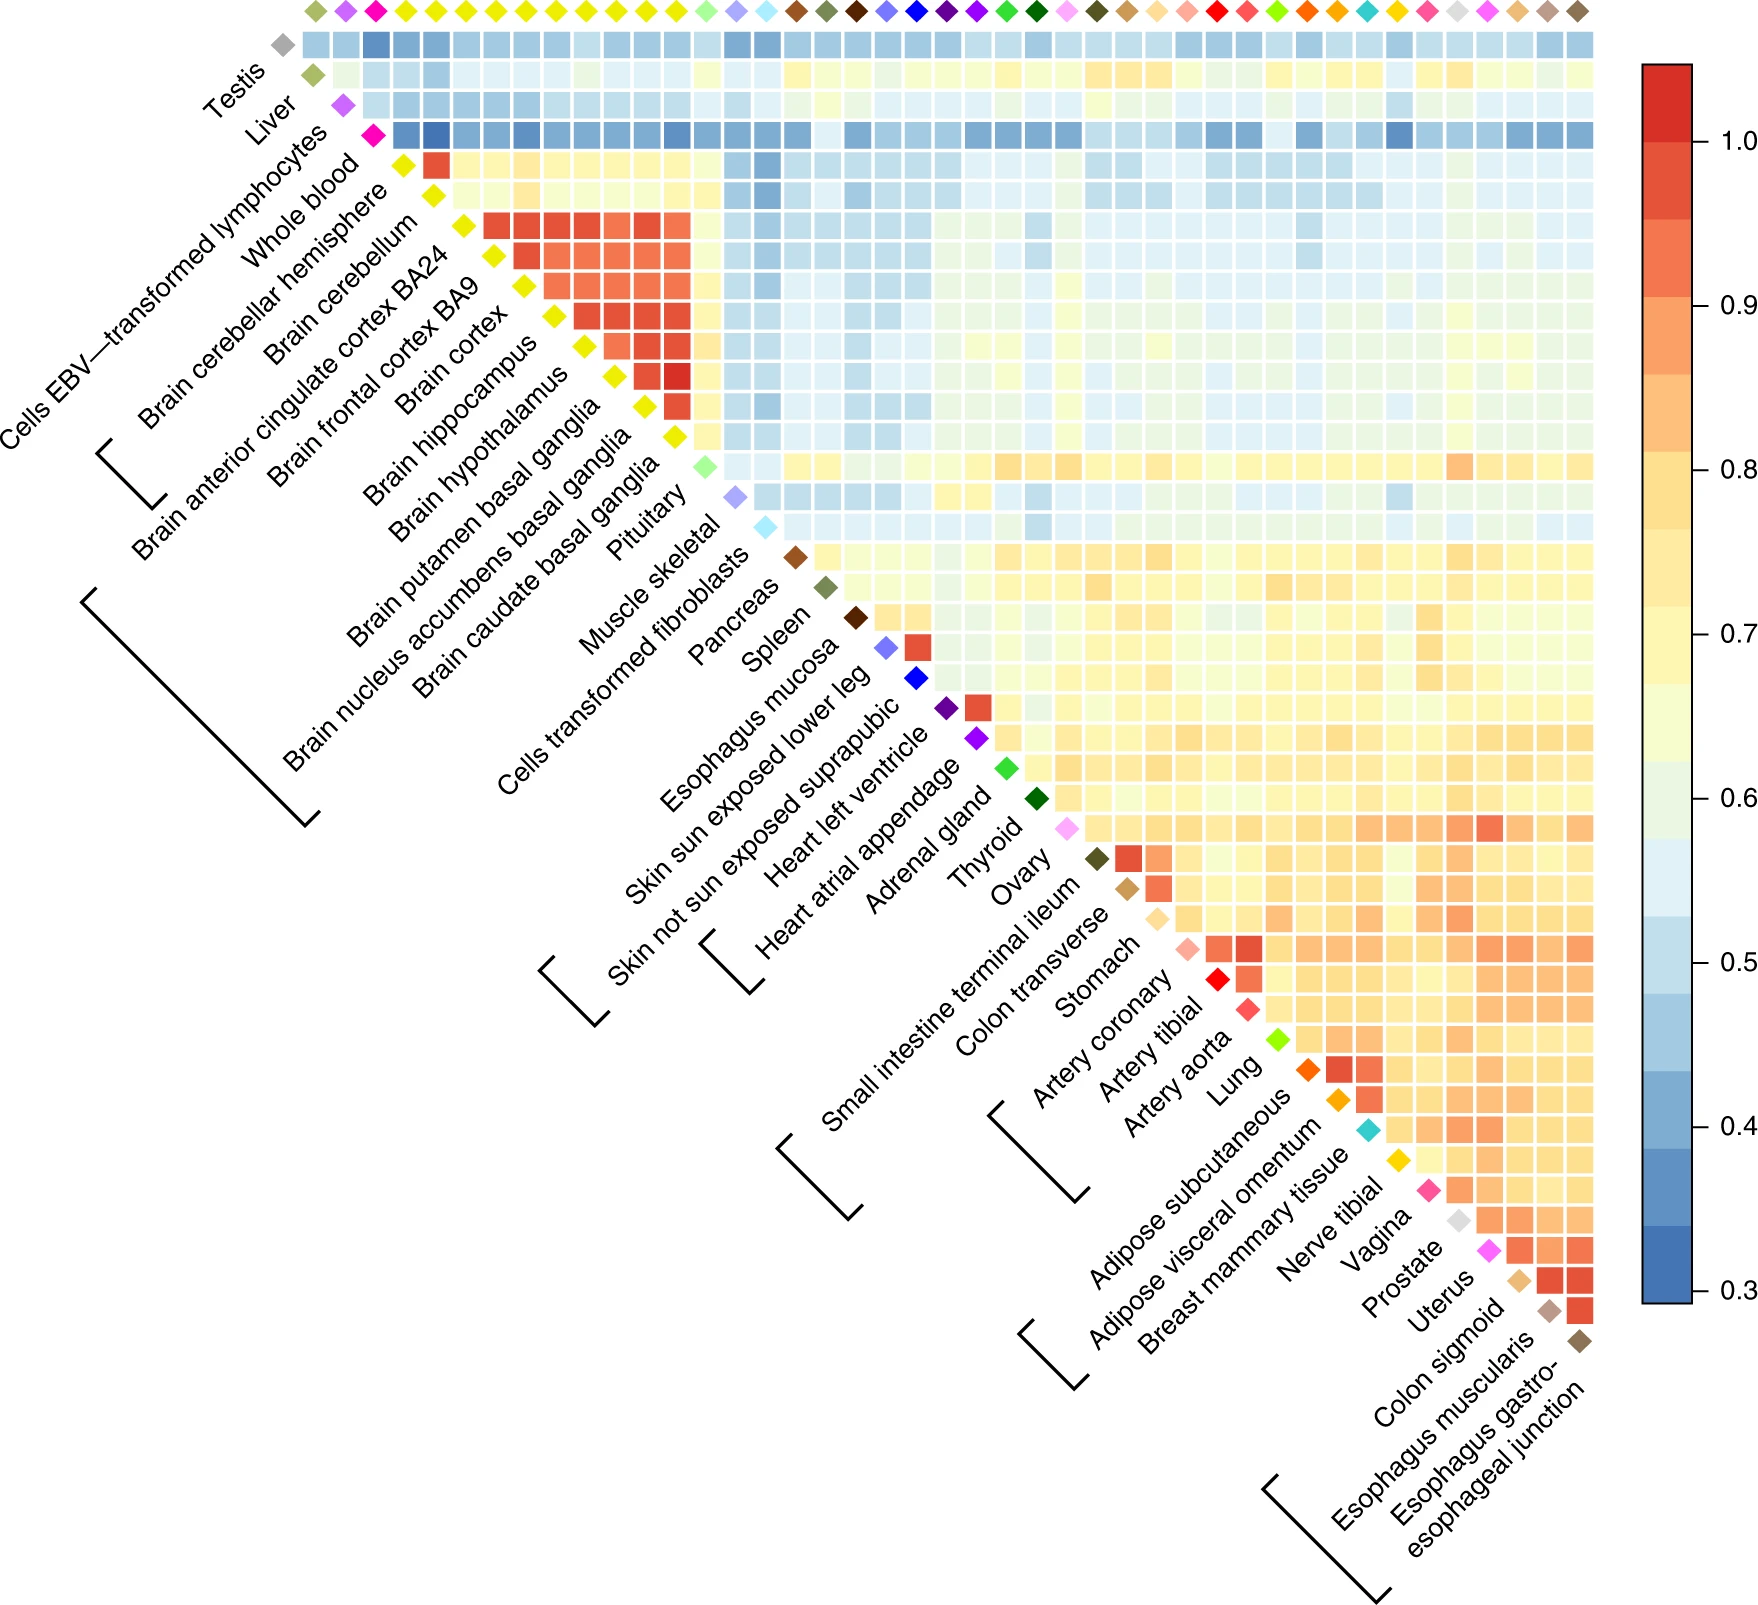
\includegraphics[width=0.62\linewidth]{slides/mash_tissue_correlation.png}
  \caption{Correlation between tissues of cis-eQTL effects in GTEx, estimated by mash. The colour scale starts at 0.3: all tissue pairs are positively correlated. Reproduced from \citet{urbut2019}.}
  \label{fig:mash_heatmap}
\end{figure}

Counting the number of tissues in which each eQTL is active gives a U-shaped distribution: most eQTLs are either specific to one or a few tissues or active in nearly all of them~\citep{gtex2017}. One explanation is the type of regulatory element. A promoter is used by its gene in every tissue in which the gene is expressed, so a promoter variant can act everywhere, while enhancers are often tissue-specific, so an enhancer variant acts only where its enhancer is active. Tissue-specific eQTLs are often shared between tissues with similar cell types. This suggests that the transcription factors that mediate eQTLs tend to be either constitutive or highly specific. Trans-eQTLs appear more tissue-specific than cis-eQTLs, although their lower power makes this hard to establish.

\subsection{Cell type composition and interaction QTLs}
\label{sec:interaction}

Most eQTL atlases are built from bulk tissue, which mixes many cell types, and the proportions vary between samples. Deconvolution methods, such as CIBERSORT (Chapter 8) or the enrichment scores of xCell~\citep{aran2017}, estimate the abundance of each cell type from expression. In GTEx they recover the expected patterns, such as hepatocytes in liver, keratinocytes in skin, myocytes in skeletal muscle, neurons in brain and neutrophils in blood, spleen and lung, and the similarity of tissues in cell type composition correlates with their similarity in eQTL and sQTL sharing~\citep{kimhellmuth2020}. Cell type composition is a major driver of variation in bulk expression between individuals.

If an eQTL acts in only one cell type, its effect in bulk tissue scales with that cell type's proportion. An \emph{interaction QTL} test looks for this,
\begin{equation}
  y_n = \mu + \beta_g g_n + \beta_c c_n + \beta_{gc}\,g_n c_n + \epsilon_n,
  \label{eq:ieqtl}
\end{equation}
where $c_n$ is the estimated proportion (or enrichment score) of the cell type in sample $n$, $\beta_c$ its effect on expression, and $\beta_{gc}$ the interaction: how much the genetic effect changes per unit change in cell type proportion. Testing $\beta_{gc}=0$ identifies cell type interacting eQTLs, many of which turn out to be cell type-specific eQTLs~\citep{kimhellmuth2020}. The test has limited power, because it depends on variation in proportions between samples and on noisy proportion estimates. Single-cell eQTL studies measure cell type-specific effects directly but are so far smaller and cover few tissues. The same interaction model applies to any measured context, such as age, sex, or a stimulus, which we meet again in Section~\ref{sec:coloc}.

%======================================================================
\section{Which variants are causal? Genomic annotations}
\label{sec:annotations}
%======================================================================

Fine-mapping one gene at a time is limited by LD. Pooling information across all genes can help, because the properties that make a variant more likely to be causal, such as lying in accessible chromatin or near the TSS, are shared. \citet{gaffney2012} built a hierarchical model that learns these properties from eQTL data and uses them as a prior for fine-mapping.

For gene $p$ with $M_p$ SNPs in its cis window, let $z_p\in\{0,1,\dots,M_p\}$ indicate the causal SNP, with $z_p=0$ if the gene has no eQTL; the model assumes at most one causal SNP per gene. Let $\va_{pm}\in\R^A$ be a vector of $A$ annotations of SNP $m$, such as indicators for overlapping a DNase I hypersensitive site, a histone mark peak or a predicted transcription factor binding site, and bins of distance to the TSS. The prior is
\begin{equation}
  \Pr(z_p\neq0) = \Pi, \qquad \Pr(z_p=m\mid z_p\neq0) = q_{pm} = \frac{\exp(\vlambda^\top\va_{pm})}{\sum_{m'=1}^{M_p}\exp(\vlambda^\top\va_{pm'})},
\end{equation}
a softmax over the SNPs in the window with annotation weights $\vlambda\in\R^A$, as in the multiclass logistic regression of Chapter 1. Holding the other annotations fixed, a SNP with annotation $a$ is $e^{\lambda_a}$ times more likely to be causal than one without, so $e^{\lambda_a}$ is the enrichment of the annotation. The data enter through the Bayes factor $\text{BF}_{pm}=p(\vy_p\mid z_p=m)/p(\vy_p\mid z_p=0)$ comparing the model in which SNP $m$ affects the expression $\vy_p\in\R^N$ of gene $p$ with the null model, computed from a single-SNP Bayesian regression. The marginal likelihood of gene $p$, relative to the null, is
\begin{equation}
  \frac{p(\vy_p\mid\Pi,\vlambda)}{p(\vy_p\mid z_p=0)} = (1-\Pi) + \Pi\sum_{m=1}^{M_p}q_{pm}\text{BF}_{pm},
\end{equation}
and the posterior probability that SNP $m$ is causal is
\begin{equation}
  r_{pm} = \Pr(z_p=m\mid\vy_p) = \frac{\Pi\,q_{pm}\text{BF}_{pm}}{(1-\Pi)+\Pi\sum_{m'}q_{pm'}\text{BF}_{pm'}}.
\end{equation}
$\Pi$ and $\vlambda$ are estimated by maximizing the product of the marginal likelihoods over all genes with EM. The E-step computes $r_{pm}$. The M-step sets $\Pi$ to the average of $\sum_m r_{pm}$ over genes and fits $\vlambda$ by maximizing $\sum_p\sum_m r_{pm}\log q_{pm}(\vlambda)$, a multiclass logistic regression in which each gene is one example, the classes are its SNPs and the labels are the soft posteriors $r_{pm}$ rather than observed causal variants. We never observe which variant is causal; the model learns from the noisy evidence summarized by the Bayes factors. The same structure is used for GWAS fine-mapping with annotations in Chapter 11.

Figure~\ref{fig:gaffney} shows the results for lymphoblastoid cell lines. SNPs in DNase I hypersensitive sites, which mark accessible chromatin, are about four times as likely to be causal as other SNPs, SNPs in H3K27ac and other active histone mark peaks are also enriched, and SNPs in regions marked by the repressive H3K27me3 are depleted. The enrichments hold for SNPs more than 5\,kb upstream of the TSS, which excludes promoters. The prior probability that a SNP is causal is highest at the TSS and falls quickly with distance, by an order of magnitude within a few tens of kilobases, and at every distance it is higher inside DNase sites. This is why a 1\,Mb window is generous for most eQTLs. Among transcription factors, SNPs in ChIP-seq peaks of factors such as JunD and NF-$\kappa$B are strongly enriched.

\begin{figure}[!htbp]
  \centering
  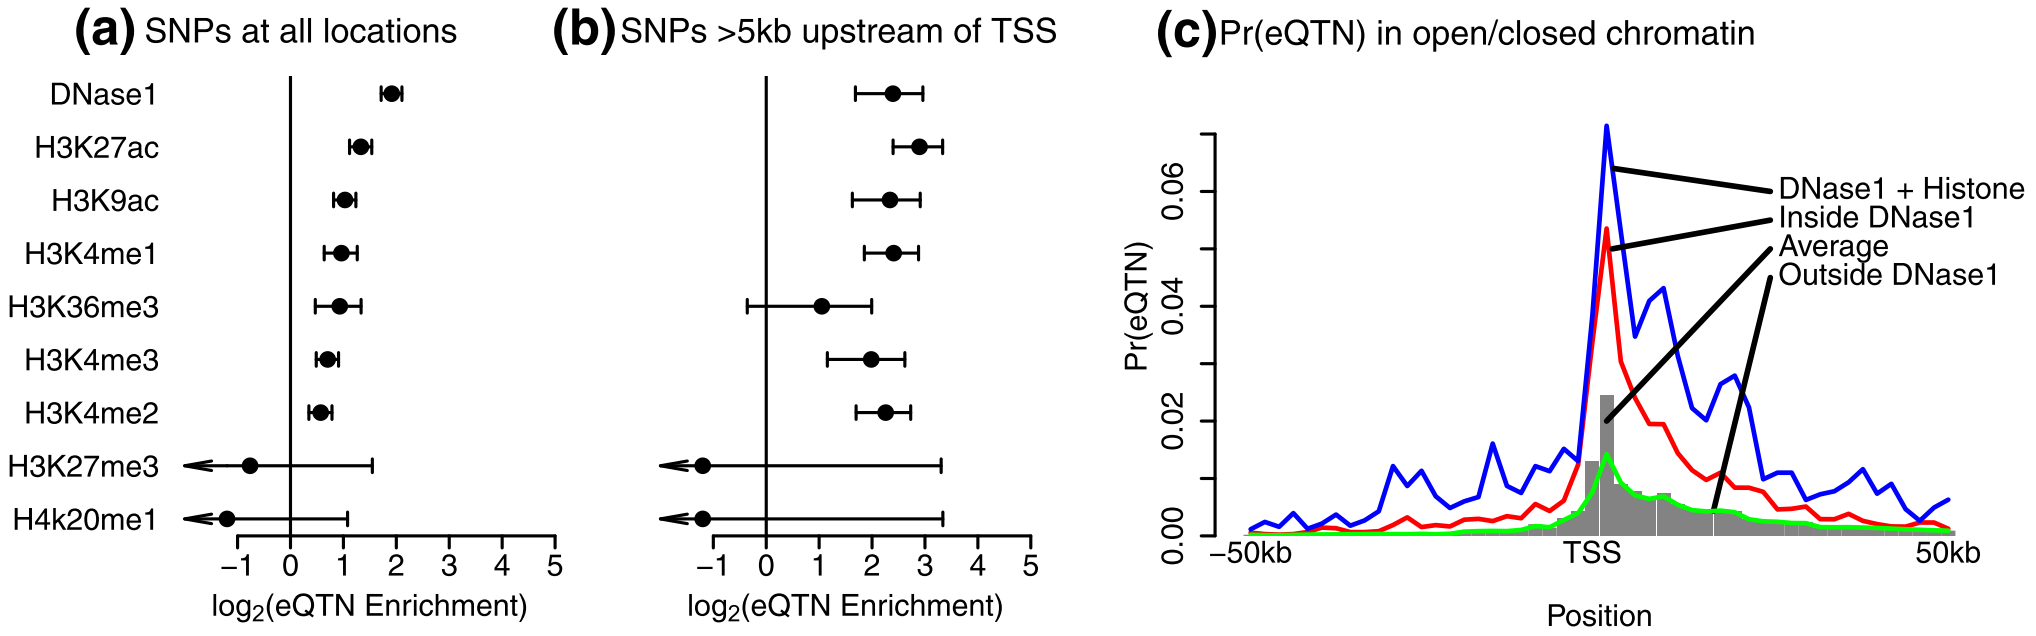
\includegraphics[width=\linewidth]{slides/gaffney_annotation_enrichment.png}
  \caption{Annotations of causal eQTL variants in lymphoblastoid cell lines. (a) Enrichment ($\log_2$, with 95\% intervals) of causal variants in DNase I hypersensitive sites and histone mark peaks, for all SNPs and (b) for SNPs more than 5\,kb upstream of the TSS. (c) Prior probability that a SNP is the causal variant as a function of position relative to the TSS, for SNPs in DNase sites and active histone marks (blue), in DNase sites (red), on average (grey) and outside DNase sites (green). Reproduced from \citet{gaffney2012}.}
  \label{fig:gaffney}
\end{figure}

Several related models exist. LirNet~\citep{lee2009lirnet} learns, across genes, how a SNP's regulatory features set the strength of its regularization in a sparse regression of expression on genotype. TORUS~\citep{wen2016} extends the hierarchical model to allow several causal SNPs per gene and controls a Bayesian FDR for eGene discovery. SuSiE~\citep{wang2020susie}, the sum of single effects model of Chapter 11, is now the most widely used fine-mapping method; it allows several causal variants, is fitted by coordinate ascent variational inference, and can take annotation-based priors such as those learned by TORUS.

Could sequence-based deep learning models (Chapters 2 and 3) replace this? Models such as Enformer predict the effects of a sequence on chromatin and expression, and so in principle predict the effect of every variant. They are good at predicting local features such as transcription factor binding and accessibility, and expression differences between genes, but not yet at predicting expression differences between individuals from their genotypes. \citet{sasse2023} compared predictions from personal genome sequences with measured brain expression: for most genes the correlation across individuals was near zero, and among genes with significant correlations, about a third had the wrong sign. The models often predict correctly that a variant matters but get the direction of its effect wrong.

%======================================================================
\section{Explaining GWAS associations with QTLs: colocalization}
\label{sec:coloc}
%======================================================================

A GWAS locus and an eQTL for a nearby gene overlap. Does that mean the gene mediates the disease association? Three questions need answers. Is there a significant eQTL in the locus at all? If so, are the GWAS and eQTL association patterns so similar that they probably share a causal variant, or could two different causal variants in LD produce overlapping signals by coincidence? And is the eQTL measured in the right tissue, cell type or cell state? \emph{Colocalization} analysis addresses the second question.

\subsection{The coloc model}

The coloc method~\citep{giambartolomei2014} considers a region of $M$ SNPs and two traits, say the expression of a gene (trait 1) and a disease (trait 2), measured in different samples. It assumes that each trait has at most one causal variant in the region, and compares five hypotheses (Figure~\ref{fig:coloc}):
\begin{itemize}
  \item $H_0$: no association with either trait;
  \item $H_1$: association with trait 1 only;
  \item $H_2$: association with trait 2 only;
  \item $H_3$: association with both traits, with two different causal variants;
  \item $H_4$: association with both traits, with one shared causal variant.
\end{itemize}
$H_4$ is what we hope to find. It does not prove that the gene causes the disease, since the shared variant could affect the disease through another gene, but it is a necessary condition. $H_3$ is the case a naive overlap analysis gets wrong.

Each hypothesis is a set of \emph{configurations}, which say which SNP, if any, is causal for each trait: one configuration for $H_0$, $M$ each for $H_1$, $H_2$ and $H_4$, and $M(M-1)$ for $H_3$. Each configuration gets a prior probability: $p_1$ for a configuration with a causal SNP for trait 1 only, $p_2$ for trait 2 only, $p_1p_2$ for two different causal SNPs, and $p_{12}$ for one shared SNP, with typical defaults $p_1=p_2=10^{-4}$ and $p_{12}=10^{-5}$. Because the two traits are measured in different samples, the likelihood factorizes over traits, and the Bayes factor of a configuration against $H_0$ is the product of a Bayes factor for each trait. Let $\text{BF}^{(1)}_m$ and $\text{BF}^{(2)}_m$ be the Bayes factors for SNP $m$ being the causal variant for traits 1 and 2. Summing over configurations, the posterior probabilities are proportional to
\begin{align}
  \Pr(H_0\mid D) &\propto 1, &
  \Pr(H_1\mid D) &\propto p_1\sum_m \text{BF}^{(1)}_m, \nonumber\\
  \Pr(H_2\mid D) &\propto p_2\sum_m \text{BF}^{(2)}_m, &
  \Pr(H_3\mid D) &\propto p_1p_2\sum_{m\neq m'}\text{BF}^{(1)}_m\text{BF}^{(2)}_{m'}, \nonumber\\
  \Pr(H_4\mid D) &\propto p_{12}\sum_m\text{BF}^{(1)}_m\text{BF}^{(2)}_m,
\end{align}
where $D$ denotes the data for both traits. The $H_3$ sum is computed as $\big(\sum_m\text{BF}^{(1)}_m\big)\big(\sum_{m'}\text{BF}^{(2)}_{m'}\big)-\sum_m\text{BF}^{(1)}_m\text{BF}^{(2)}_m$. $H_4$ wins when both traits put their Bayes factor mass on the same SNPs, and $H_3$ wins when they put it on different SNPs.

The Bayes factors need only summary statistics. Let $\hat\beta_m$ be the estimated effect of SNP $m$ on a trait, with sampling variance $V_m=\text{se}(\hat\beta_m)^2$, so $\hat\beta_m\mid\beta_m\sim\Normal(\beta_m,V_m)$. Under the null $\beta_m=0$, and under the alternative $\beta_m\sim\Normal(0,W)$ with prior variance $W$, so marginally $\hat\beta_m\sim\Normal(0,V_m+W)$. The ratio of the two densities is Wakefield's approximate Bayes factor~\citep{wakefield2009},
\begin{equation}
  \text{BF}_m = \frac{\Normal(\hat\beta_m;0,V_m+W)}{\Normal(\hat\beta_m;0,V_m)} = \sqrt{\frac{V_m}{V_m+W}}\exp\left(\frac{z_m^2}{2}\,\frac{W}{V_m+W}\right),
  \label{eq:abf-12}
\end{equation}
where $z_m=\hat\beta_m/\sqrt{V_m}$. It increases with $z_m^2$, and the prefactor penalizes the alternative for spreading its prior over effects that the data could have shown but did not. Under the single-causal-variant assumption, the Bayes factor of the configuration ``SNP $m$ is causal'' is $\text{BF}_m$ computed from the marginal statistics of SNP $m$ alone, so no LD matrix is needed. The assumption is restrictive when a locus has several causal variants; extensions combine coloc with SuSiE fine-mapping to test each pair of credible sets.

Figure~\ref{fig:coloc} shows coloc on simulated data, with an eQTL study of 500 individuals and a GWAS of 5000. When the same SNP is causal for both traits, the association patterns match and the posterior probability of $H_4$ is 0.99. When the GWAS causal variant is a different SNP in weak LD ($r^2=0.31$) with the eQTL causal variant, both traits show associations across the same region, but their peaks are at different SNPs, and the posterior probability of $H_3$ is 0.94.

\begin{figure}[!htbp]
  \centering
  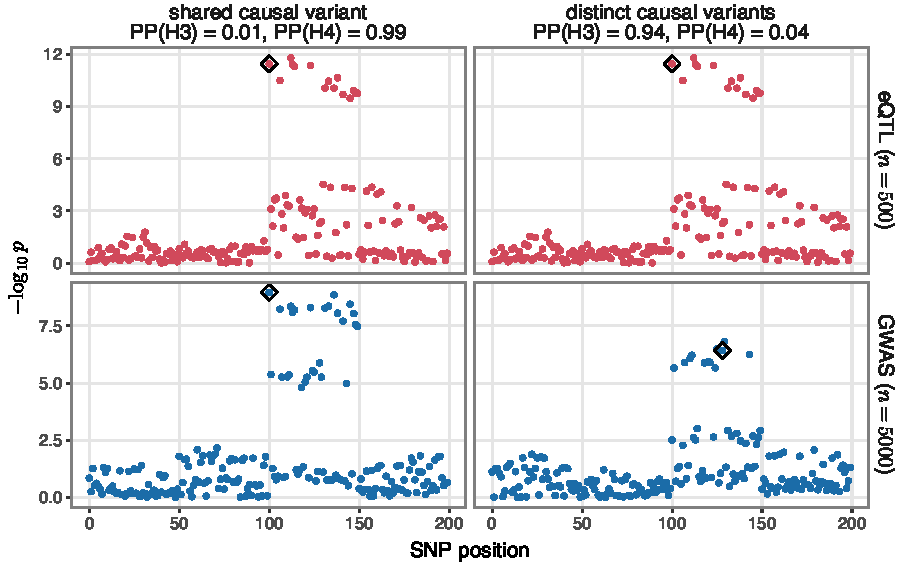
\includegraphics[width=0.9\linewidth]{coloc_example.pdf}
  \caption{Colocalization on simulated data. Association $-\log_{10}p$ along a region of 200 SNPs for an eQTL ($N=500$, red) and a GWAS ($N=5000$, blue); diamonds mark the causal variants. Left, one shared causal variant; right, distinct causal variants in weak LD. Panel titles give the coloc posterior probabilities of $H_3$ and $H_4$ with default priors and $W=0.15^2$.}
  \label{fig:coloc}
\end{figure}

\subsection{What colocalization has found}

The GTEx consortium ran colocalization for GWAS of many traits, including lipid levels, BMI and autoimmune diseases~\citep{gtex2017}. A substantial fraction of GWAS loci colocalize with an eQTL in at least one tissue, and the colocalizing gene is often not the gene nearest to the lead GWAS variant, as for \textit{FTO}, \textit{IRX3} and \textit{IRX5}. Many loci, however, do not colocalize with any eQTL. Some of this gap is power, but some is because eQTL studies measure the wrong context. Expression effects relevant to an immune disease may only appear when immune cells respond to a challenge, while blood samples contain mostly resting cells. \citet{kimhellmuth2017} stimulated monocytes from 134 donors with bacterial and viral ligands and found eQTLs that appeared only after stimulation, some of which colocalized with autoimmune disease associations that resting-cell eQTLs did not explain. The cell state can matter, not just the cell type.

Why does this matter? Drug targets with human genetic support are more likely to succeed in clinical trials (Chapter 1). The effects involved are small: a typical eQTL changes expression by perhaps 5--10\%, and each GWAS variant changes disease risk slightly, so these results are of little use for predicting who will get a disease. They do give a view of the causal biology of disease in humans, without the limitations of animal models and without a clinical trial.

%======================================================================
\section{Transcriptome-wide association studies}
%======================================================================

A transcriptome-wide association study (TWAS)~\citep{gamazon2015,gusev2016} links expression to a trait through genetically predicted expression (Figure~\ref{fig:twas}). In a \emph{reference panel} with genotypes and expression, we train a model to predict each gene's expression from the genotypes of its cis SNPs,
\begin{equation}
  e_n = \vx_n^\top\vw + \epsilon_n,
\end{equation}
where $e_n$ is the expression of the gene in individual $n$ of the panel, $\vx_n\in\R^M$ holds the standardized genotypes of the $M$ cis SNPs and $\vw\in\R^M$ the weights, usually fitted with the elastic net or lasso of Chapter 1, or with a Bayesian sparse regression. In a GWAS cohort, which has genotypes and the trait but no expression, we then impute expression, $\hat e_n=\vx_n^\top\hat\vw$, and test the association between $\hat e_n$ and the trait.

\begin{figure}[!htbp]
  \centering
  \begin{tikzpicture}[>=Stealth, every node/.style={font=\small},
      mat/.style={draw, minimum width=1.6cm, minimum height=1.0cm, align=center, fill=gray!8}]
    \node[mat] (gref) at (0,0) {cis SNPs\\$\mX_{\text{ref}}$};
    \node[mat, fill=red!10, minimum width=0.8cm] (eref) at (2.2,0) {$\ve$};
    \node at (1.2,0) {$\sim$};
    \node[above] at (1.1,0.6) {reference panel};
    \draw[->, thick] (2.2,-0.6) -- (2.2,-1.3) node[midway, right] {fit $\hat\vw$};
    \node[mat] (ggw) at (0,-2.4) {cis SNPs\\$\mX_{\text{GWAS}}$};
    \node[mat, fill=red!5, minimum width=0.8cm, dashed] (ehat) at (2.2,-2.4) {$\hat\ve$};
    \node[mat, fill=blue!8, minimum width=0.8cm] (trait) at (3.8,-2.4) {trait\\$\vy$};
    \draw[->] (gref.south) -- (ggw.north) node[midway, left] {\footnotesize same SNPs};
    \draw[->, thick] (ggw) -- (ehat) node[midway, above] {\footnotesize$\hat\vw$};
    \node at (3.0,-2.4) {$\sim$};
    \node[below, align=center] at (1.9,-3.1) {individual-level TWAS};
    % summary based
    \node[mat, minimum width=2.4cm] (z) at (7.4,-0.2) {GWAS $z$ scores\\$z_1,\dots,z_M$};
    \node[mat, minimum width=2.4cm] (ld) at (7.4,-1.6) {LD reference\\$\mSigma$};
    \node[mat, fill=red!5, dashed, minimum width=2.6cm] (zt) at (7.4,-3.0) {$z_{\text{TWAS}}=\dfrac{\hat\vw^\top\vz}{\sqrt{\hat\vw^\top\mSigma\hat\vw}}$};
    \draw[->] (z) -- (ld); \draw[->] (ld) -- (zt);
    \node[above] at (7.4,0.45) {summary-based TWAS};
    \draw[dashed, gray] (5.2,0.8) -- (5.2,-3.6);
  \end{tikzpicture}
  \caption{Transcriptome-wide association study. Left: weights $\hat\vw$ predicting a gene's expression from cis SNPs are learned in a reference panel, used to impute expression in a GWAS cohort, and imputed expression is tested for association with the trait. Right: the same test computed from GWAS summary statistics and an LD reference. After \citet{gusev2016}.}
  \label{fig:twas}
\end{figure}

Individual-level GWAS data are often unavailable, but the test can be computed from GWAS summary statistics~\citep{gusev2016}. Let $\mX\in\R^{N\times M}$ be the standardized cis genotypes of the $N$ GWAS individuals and $\vy\in\R^N$ the standardized trait. The marginal $z$ score of SNP $m$ is approximately $z_m=\vx_m^\top\vy/\sqrt N$, where $\vx_m$ is column $m$ of $\mX$, so $\vz=\mX^\top\vy/\sqrt N$. The imputed expression is $\hat\ve=\mX\hat\vw$, with sample variance $\hat\vw^\top\mSigma\hat\vw$, where $\mSigma=\mX^\top\mX/N$ is the LD (correlation) matrix of the SNPs. The $z$ score for the association of $\hat\ve$ with $\vy$ is
\begin{equation}
  z_{\text{TWAS}} = \frac{\hat\ve^\top\vy}{\sqrt N\sqrt{\hat\vw^\top\mSigma\hat\vw}} = \frac{\hat\vw^\top\mX^\top\vy/\sqrt N}{\sqrt{\hat\vw^\top\mSigma\hat\vw}} = \frac{\hat\vw^\top\vz}{\sqrt{\hat\vw^\top\mSigma\hat\vw}},
  \label{eq:twas}
\end{equation}
a weighted sum of the GWAS $z$ scores, normalized by its null standard deviation: under the null $\vz\sim\Normal(\vzero,\mSigma)$, so $\Var(\hat\vw^\top\vz)=\hat\vw^\top\mSigma\hat\vw$. The LD matrix comes from a reference sample of the same ancestry.

TWAS has two attractions. It is signed: the sign of $z_{\text{TWAS}}$ says whether higher genetically predicted expression increases or decreases risk, which is what we need to know to design a drug that inhibits or activates a target. And it is protected against reverse causation. Expression measured in patients reflects the disease as well as causing it; in Alzheimer's disease, for example, microglia in the brain respond to the damage, so much of the expression difference between cases and controls is a consequence of the disease. Genetically predicted expression is fixed at conception and cannot be changed by the disease.

Figure~\ref{fig:twas_pd} shows a TWAS of Parkinson's disease~\citep{li2018leafcutter}, using 537 dorsolateral prefrontal cortex RNA-seq samples from the CommonMind consortium~\citep{fromer2016} as the reference panel and a GWAS of about 14{,}000 cases and 95{,}000 controls~\citep{nalls2014}. With predicted splicing (intron usage quantified by LeafCutter, Chapter 10) as well as predicted expression, 26 genes were associated through splicing and 18 through expression at 5\% FDR. The strongest signal was splicing of \textit{MAPT}, which encodes tau.

\begin{figure}[!htbp]
  \centering
  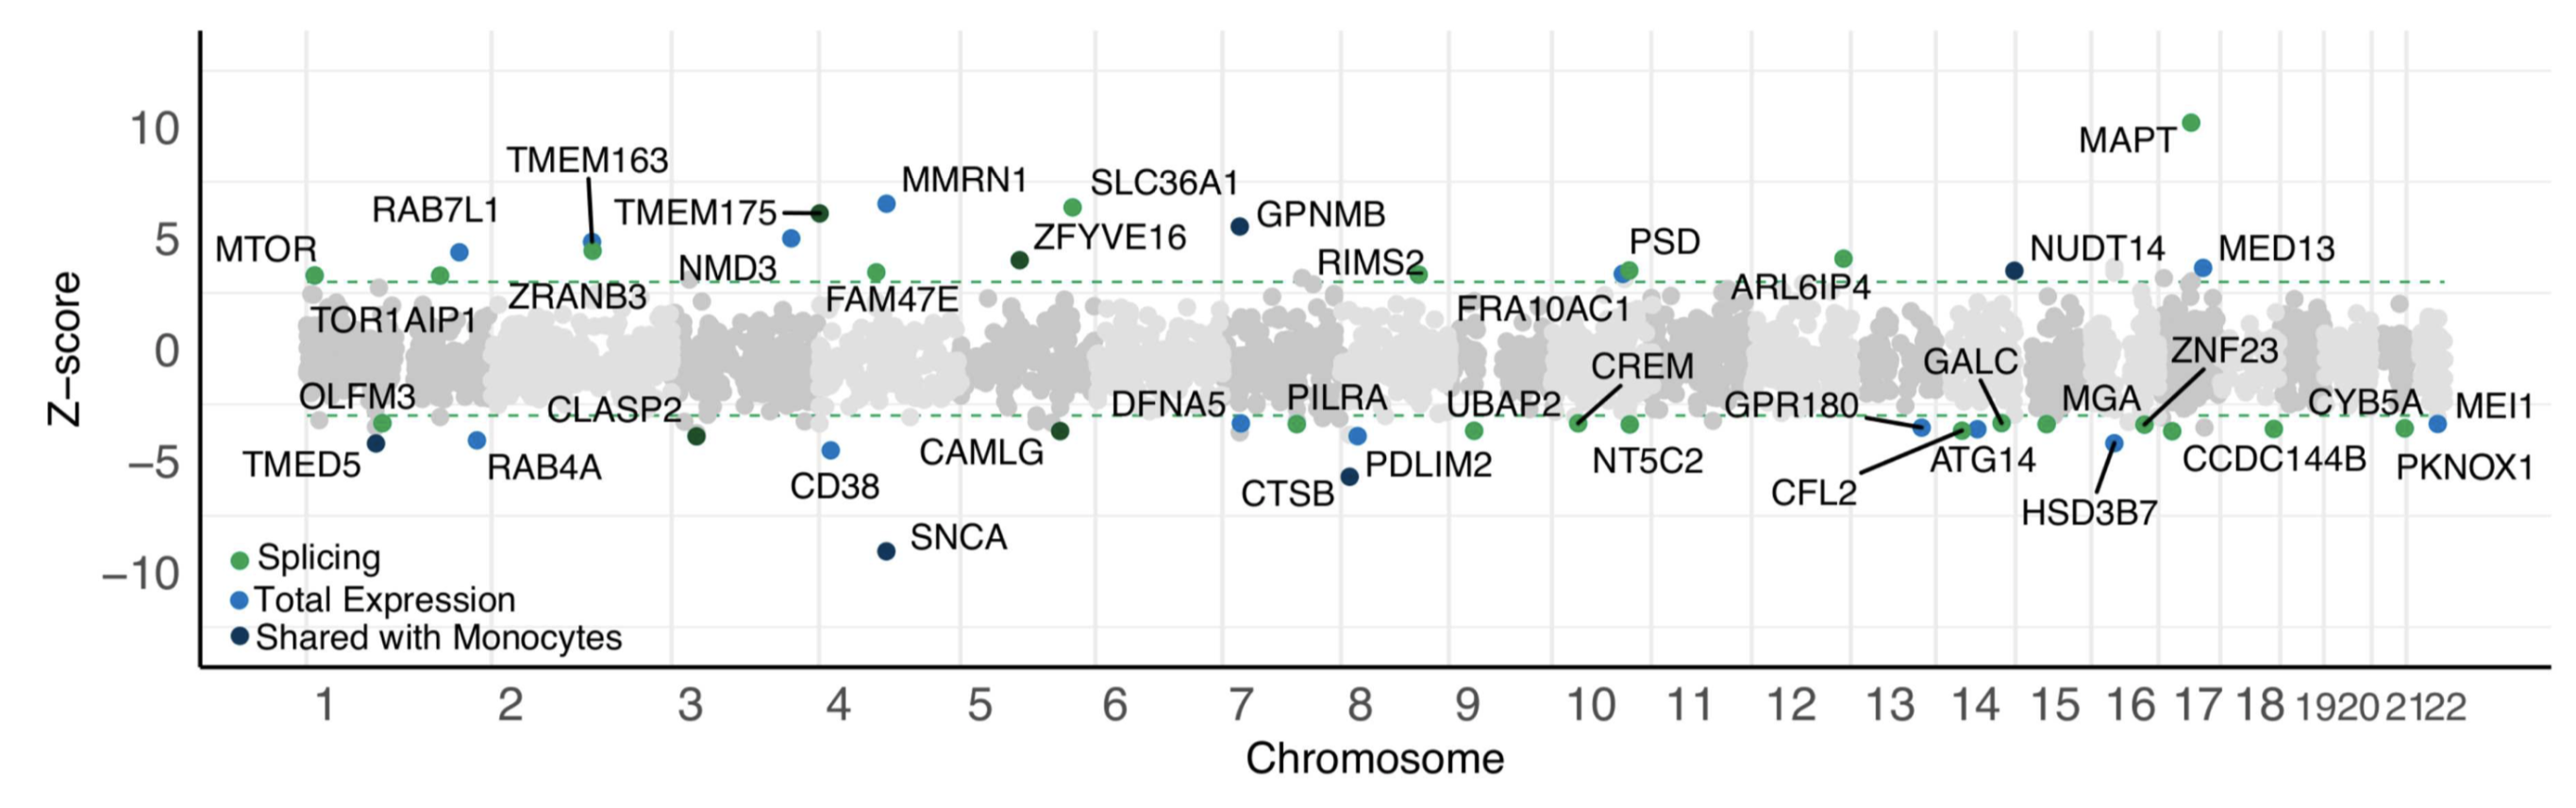
\includegraphics[width=0.85\linewidth]{slides/twas_parkinsons.png}
  \caption{TWAS of Parkinson's disease using brain expression (blue) and splicing (green) reference panels; dark points are associations shared with monocytes. Each point is a gene's TWAS $z$ score along the genome; dashed lines mark significance at 5\% FDR. Reproduced from \citet{li2018leafcutter}.}
  \label{fig:twas_pd}
\end{figure}

TWAS inherits the limitations of its components. Genes in the same locus have correlated predicted expression, because they share cis SNPs and LD, so a TWAS association, like an overlapping eQTL, can be driven by a neighbouring gene or by a variant acting through another mechanism. TWAS assumes the variants in the predictor affect the trait only through the gene's expression. This is the central assumption of Mendelian randomization, to which TWAS is closely related.

%======================================================================
\section{Mendelian randomization}
%======================================================================

\subsection{Instrumental variables}

Mendelian randomization (MR)~\citep{daveysmith2003} estimates the causal effect of an \emph{exposure} $X$, such as the expression of a gene or a biomarker like LDL cholesterol, on an \emph{outcome} $Y$, such as disease risk. The problem is the usual one of observational data: an association between $X$ and $Y$ can be due to a confounder $U$ that affects both, or to reverse causation. MR uses a genetic variant $G_j$ associated with the exposure as an \emph{instrumental variable} (Figure~\ref{fig:mr_dag}). Alleles are assigned at random at conception, given the parents' genotypes, much as treatments are in a randomized trial, hence the name. The instrument is valid under three assumptions:
\begin{enumerate}
  \item \emph{relevance}: $G_j$ is associated with $X$;
  \item \emph{independence}: $G_j$ is not associated with any confounder $U$ of $X$ and $Y$;
  \item \emph{exclusion restriction}: $G_j$ affects $Y$ only through $X$, with no direct (pleiotropic) path.
\end{enumerate}
In an eQTL setting, the exposure is the expression of a gene and the instrument is a cis-eQTL, which makes the first assumption easy to check and the third plausible but not guaranteed.

\begin{figure}[!htbp]
  \centering
  \begin{tikzpicture}[>=Stealth, every node/.style={font=\small}, var/.style={draw, rounded corners, minimum width=1.5cm, minimum height=0.7cm, align=center}]
    \node[var, fill=green!12] (g) at (0,0) {SNP $G_j$\\(instrument)};
    \node[var, fill=blue!10] (x) at (4,0) {exposure $X$};
    \node[var, fill=red!10] (y) at (8,0) {outcome $Y$};
    \node[var, fill=orange!20] (u) at (6,1.8) {confounder $U$};
    \draw[->, thick] (g) -- node[above] {$\gamma_j$} (x);
    \draw[->, thick] (x) -- node[above] {$\beta$} (y);
    \draw[->] (u) -- (x); \draw[->] (u) -- (y);
    \draw[->, dashed, gray] (g.north) to[out=50, in=180] node[midway, above, black] {$\times$} (u.west);
    \draw[->, dashed, gray] (g.south) to[out=-25, in=-155] node[midway, below, black] {$\times$ \ $\alpha_j$} (y.south);
  \end{tikzpicture}
  \caption{Mendelian randomization. A SNP $G_j$ affects the exposure $X$ with effect $\gamma_j$, and $X$ affects the outcome $Y$ with causal effect $\beta$. The SNP must not be associated with the confounder $U$, and must have no direct effect $\alpha_j$ on the outcome (crossed dashed paths).}
  \label{fig:mr_dag}
\end{figure}

\subsection{The ratio estimate}

Write a linear model for the exposure and the outcome,
\begin{equation}
  X = \gamma_jG_j + U + \epsilon_X, \qquad Y = \beta X + \alpha_jG_j + \kappa U + \epsilon_Y,
\end{equation}
where $\gamma_j$ is the effect of SNP $j$ on the exposure, $\beta$ the causal effect of the exposure on the outcome, $\alpha_j$ a direct (pleiotropic) effect of the SNP on the outcome, $\kappa$ the effect of the confounder, and $\epsilon_X,\epsilon_Y$ independent noise. Under the independence assumption $\Cov(G_j,U)=0$, so
\begin{align}
  \Cov(G_j,X) &= \gamma_j\Var(G_j), \\
  \Cov(G_j,Y) &= \beta\Cov(G_j,X) + \alpha_j\Var(G_j) = (\beta\gamma_j+\alpha_j)\Var(G_j).
\end{align}
The regression coefficients of the exposure and the outcome on the SNP are therefore $\gamma_j$ and $\Gamma_j=\beta\gamma_j+\alpha_j$, and these are exactly what GWAS of the exposure and of the outcome estimate. The confounder has dropped out. If the exclusion restriction holds, $\alpha_j=0$ and the \emph{ratio} (Wald) estimate
\begin{equation}
  \hat\beta_j = \frac{\hat\Gamma_j}{\hat\gamma_j} = \frac{\hat\beta_{\text{SNP}\to\text{outcome}}}{\hat\beta_{\text{SNP}\to\text{exposure}}}
\end{equation}
is a consistent estimate of $\beta$. With pleiotropy it estimates $\beta+\alpha_j/\gamma_j$, biased by an amount that is larger for weaker instruments.

\subsection{Multiple instruments}

With $J$ independent instruments (SNPs not in LD with each other), the inverse-variance weighted (IVW) estimate~\citep{burgess2013} combines the ratio estimates. Treating $\hat\gamma_j$ as known and $\text{se}(\hat\beta_j)\approx\text{se}(\hat\Gamma_j)/|\hat\gamma_j|$, weighting each ratio by its inverse variance gives
\begin{equation}
  \hat\beta_{\text{IVW}} = \frac{\sum_j \hat\beta_j\,\hat\gamma_j^2\sigma_j^{-2}}{\sum_j\hat\gamma_j^2\sigma_j^{-2}} = \frac{\sum_j\hat\gamma_j\hat\Gamma_j\sigma_j^{-2}}{\sum_j\hat\gamma_j^2\sigma_j^{-2}},
\end{equation}
where $\sigma_j=\text{se}(\hat\Gamma_j)$. This is the weighted least-squares slope of a regression of $\hat\Gamma_j$ on $\hat\gamma_j$ through the origin. If the pleiotropic effects $\alpha_j$ average to zero (balanced pleiotropy), IVW is still consistent. If they do not (directional pleiotropy, mean $\mu_\alpha\neq0$), IVW is biased.

MR-Egger regression~\citep{bowden2015} relaxes the assumption. Writing $\alpha_j=\mu_\alpha+(\alpha_j-\mu_\alpha)$,
\begin{equation}
  \Gamma_j = \mu_\alpha + \beta\gamma_j + (\alpha_j-\mu_\alpha).
\end{equation}
If the pleiotropic effects are independent of the instrument strengths $\gamma_j$ across SNPs (the InSIDE assumption, instrument strength independent of direct effect), the last term is uncorrelated with $\gamma_j$, and a weighted regression of $\hat\Gamma_j$ on $\hat\gamma_j$ \emph{with an intercept} estimates the causal effect $\beta$ as its slope and the average pleiotropy $\mu_\alpha$ as its intercept. Before fitting, each SNP is oriented so that $\hat\gamma_j>0$; otherwise the intercept would depend on the arbitrary choice of reference allele. A non-zero intercept is evidence of directional pleiotropy. Figure~\ref{fig:mr_egger} shows simulated data in which all SNPs have a small positive direct effect on the outcome: IVW overestimates the causal effect (0.30 against a true 0.2), while the Egger slope is closer (0.24) and its intercept (0.012) estimates the mean direct effect (0.018 in this sample).

\begin{figure}[!htbp]
  \centering
  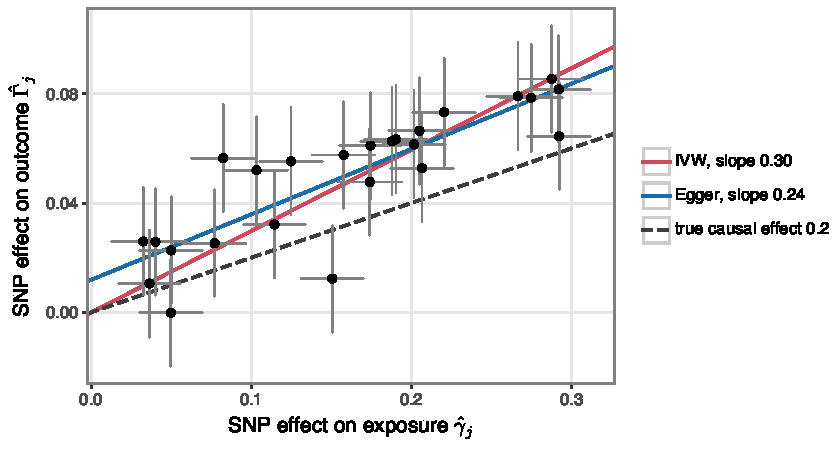
\includegraphics[width=0.8\linewidth]{mr_egger.pdf}
  \caption{IVW and Egger regression on 25 simulated instruments with directional pleiotropy. Each point is a SNP's estimated effects on the exposure and the outcome, with 95\% intervals. IVW (red) is a regression through the origin and is biased by the positive direct effects; Egger regression (blue) has an intercept and its slope is closer to the true causal effect (dashed).}
  \label{fig:mr_egger}
\end{figure}

The InSIDE assumption fails when pleiotropy is \emph{correlated}: if some SNPs affect both exposure and outcome through a shared heritable factor, their direct effects are correlated with their effects on the exposure, and the Egger slope is biased too. CAUSE~\citep{morrison2020} models a mixture of SNPs with and without such shared effects, and Welch-weighted Egger regression~\citep{brown2021welch} reduces the resulting false positives. All these methods need several valid or nearly valid instruments, and molecular exposures often have only one or two strong cis instruments.

TWAS and MR are closely related. The TWAS statistic~\eqref{eq:twas} is a weighted combination of SNP-outcome associations with weights from the SNP-exposure model, and with a single SNP it is the GWAS $z$ score of that SNP, whose ratio to the eQTL effect is the MR estimate. TWAS tests $\beta=0$ while MR estimates $\beta$, and both rely on the exclusion restriction.

\subsection{Causal networks}

Molecular phenotypes come in large numbers: thousands of genes, splicing events, proteins and metabolites, as well as complex traits. MR between every pair gives a matrix of pairwise causal effect estimates, but these are \emph{total} effects, which include all paths through other phenotypes. We would often rather know the \emph{direct} effects, the edges of a causal network (Figure~\ref{fig:networks}).

\begin{figure}[!htbp]
  \centering
  \begin{tikzpicture}[>=Stealth, every node/.style={font=\small}, nd/.style={circle, draw, fill=blue!15, minimum size=0.7cm}]
    \begin{scope}
      \node[above] at (1.5,1.3) {direct effects $\mG$};
      \node[nd, fill=orange!30] (a) at (0,0) {$A$};
      \node[nd] (b) at (1.5,0.9) {$B$};
      \node[nd] (c) at (1.5,-0.9) {$C$};
      \node[nd, fill=yellow!40, diamond, inner sep=1pt] (d) at (3.0,0) {$D$};
      \draw[->, thick] (a) -- (b); \draw[->, thick] (a) -- (c);
      \draw[->, thick] (c) -- (b); \draw[->, thick] (b) -- (d);
    \end{scope}
    \begin{scope}[xshift=6cm]
      \node[above] at (1.5,1.3) {total effects $\mR=(\mI-\mG)^{-1}$};
      \node[nd, fill=orange!30] (a) at (0,0) {$A$};
      \node[nd] (b) at (1.5,0.9) {$B$};
      \node[nd] (c) at (1.5,-0.9) {$C$};
      \node[nd, fill=yellow!40, diamond, inner sep=1pt] (d) at (3.0,0) {$D$};
      \draw[->, thick] (a) -- (b); \draw[->, thick] (a) -- (c);
      \draw[->, thick] (c) -- (b); \draw[->, thick] (b) -- (d);
      \draw[->, dotted, thick] (a) -- (d);
      \draw[->, dotted, thick] (c) to[out=10, in=-100] (d);
    \end{scope}
  \end{tikzpicture}
  \caption{Direct and total effects. Left, a network of direct causal effects in which a transcription factor $A$ regulates genes $B$ and $C$, $C$ regulates $B$, and $B$ affects a trait $D$. Right, the total effects estimated by pairwise MR include indirect effects (dotted), such as $A$ on $D$ through $B$, and $A$ on $B$ both directly and through $C$.}
  \label{fig:networks}
\end{figure}

A linear structural model relates the two. Let $\mY\in\R^{N\times D}$ hold $D$ phenotypes for $N$ individuals and $\mG\in\R^{D\times D}$ the direct effects, with $G_{ij}$ the effect of phenotype $i$ on phenotype $j$ and $G_{ii}=0$. Each phenotype is a linear function of the others plus external perturbations $\mE\in\R^{N\times D}$, which include the effects of genetic instruments and environment,
\begin{equation}
  \mY = \mY\mG + \mE \quad\Rightarrow\quad \mY(\mI-\mG) = \mE \quad\Rightarrow\quad \mY = \mE(\mI-\mG)^{-1}.
\end{equation}
A unit perturbation of phenotype $i$ (row vector $\mE$ with a one in position $i$) therefore changes phenotype $j$ by $[(\mI-\mG)^{-1}]_{ij}$, the total effect. When the network has no feedback loops strong enough to make the series diverge,
\begin{equation}
  (\mI-\mG)^{-1} = \mI + \mG + \mG^2 + \mG^3 + \cdots,
\end{equation}
and $[\mG^2]_{ij}=\sum_kG_{ik}G_{kj}$ sums the paths of length two from $i$ to $j$. In the network of Figure~\ref{fig:networks}, the total effect of $A$ on $B$ is $G_{AB}+G_{AC}G_{CB}$, the direct edge plus the path through $C$, and the total effect of $A$ on $D$ is $(G_{AB}+G_{AC}G_{CB})G_{BD}$.

MR estimates the total effect of a perturbation that changes $i$ by one unit, so the matrix of MR estimates is $\mR=\mD^{-1}(\mI-\mG)^{-1}$ with $\mD$ the diagonal of $(\mI-\mG)^{-1}$, normalizing each row so that $R_{ii}=1$. Then $\mR^{-1}=(\mI-\mG)\mD$, whose off-diagonal entries are $-G_{ij}D_{jj}$ and diagonal entries $D_{ii}$. A sparse network $\mG$ therefore means a sparse inverse of $\mR$, and the direct effects are recovered as $G_{ij}=-[\mR^{-1}]_{ij}/[\mR^{-1}]_{jj}$. Inverting a noisy estimate $\hat\mR$ directly amplifies the noise, so bimmer~\citep{brown2020bimmer} and its successor inspre~\citep{brown2023inspre} solve a regularized problem,
\begin{equation}
  \min_{\mU,\mV}\ \sum_{i,j}w_{ij}\big(\hat R_{ij}-U_{ij}\big)^2 + \lambda\|\mV\|_1 \quad\text{subject to}\quad \mU\mV=\mI,
\end{equation}
where $\mU\in\R^{D\times D}$ is a denoised version of $\hat\mR$, $\mV=\mU^{-1}$ is its sparse inverse, $w_{ij}\geq0$ are weights reflecting the precision of each MR estimate (zero for missing entries), and $\|\mV\|_1=\sum_{ij}|V_{ij}|$. The problem is biconvex (convex in $\mU$ for fixed $\mV$ and vice versa) and is solved with the alternating direction method of multipliers (ADMM)~\citep{boyd2011admm}. It is the directed analogue of the graphical lasso of Chapter 9~\citep{friedman2008}, which finds a sparse inverse of a covariance matrix, and $\lambda$ is chosen by a stability criterion adapted from StARS~\citep{liu2010stars}. In simulations of random, hub-like and scale-free directed networks, this approach recovers the network much more accurately than estimating each node's parents by sparse regression on pairwise MR estimates. Applied with CRISPR knockdowns as the perturbations instead of genetic instruments, the same method estimates gene regulatory networks from Perturb-seq data~\citep{brown2023inspre}.

%======================================================================
\section{Summary}
%======================================================================

\begin{itemize}
  \item Molecular QTLs are associations between genotype and molecular phenotypes such as expression (eQTLs), splicing (sQTLs) and chromatin accessibility (caQTLs). They help interpret GWAS loci, most of which are non-coding, by suggesting causal genes, tissues and cell types, as in the \textit{FTO} locus, where the obesity variants regulate \textit{IRX3} and \textit{IRX5} in adipocyte progenitors.
  \item eQTLs are mapped by linear regression of normalized expression on genotype, usually for SNPs within 1\,Mb of each gene. Multiple testing is handled at two levels: within a gene by Bonferroni or permutation, which accounts for LD, and across genes by FDR control.
  \item Technical and biological confounders affect many genes at once and can be estimated as hidden factors with a factor model with an ARD prior (PEER) or by PCA. Regressing them out greatly increases power for cis-eQTLs but can remove trans signals and context-specific biology.
  \item Cis-eQTLs are common, large and easy to find with tens to hundreds of individuals; trans-eQTLs are small and need thousands. LD makes the causal variant hard to identify; fine-mapping and genome-wide annotation enrichment, which shows causal variants concentrated in accessible chromatin near the TSS, help.
  \item Allele-specific expression compares the two haplotypes within an individual, a built-in control for environmental and technical variation that isolates cis effects. Overdispersed counts are modelled with the beta-binomial (allelic counts) and negative binomial (total counts), and combining the two signals gains power, especially in small samples. QQ plots check calibration.
  \item Tissue atlases show that most genes have cis-eQTLs, often several, that eQTLs are mostly either shared across tissues or specific to a few, and that comparing significance between tissues is misleading; mash models effects jointly. Cell type composition shapes bulk eQTLs, and interaction models can recover cell type-specific effects.
  \item Colocalization tests whether a GWAS and an eQTL signal share a causal variant; TWAS associates genetically predicted expression with a trait; Mendelian randomization estimates causal effects using SNPs as instrumental variables, with Egger and related methods relaxing the no-pleiotropy assumption. Extending MR to many phenotypes leads to sparse causal network inference.
\end{itemize}

%======================================================================
\section*{Exercises}
%======================================================================

\begin{enumerate}
  \item Show that under the null, with $M$ independent SNPs, $\Pr(p_{\min}\leq t)=1-(1-t)^M$, and that the Bonferroni threshold $t=0.05/M$ gives a family-wise error rate between 0.0488 and 0.05 for all $M\geq1$.
  \item Starting from~\eqref{eq:betabinom}, show that $\Pr(y\mid d,\mu,c)\to\binom{d}{y}\mu^y(1-\mu)^{d-y}$ as $c\to\infty$ with $\mu$ fixed. Show similarly that $\NB(y\mid m,\phi)\to\Pois(y\mid m)$ as $\phi\to\infty$.
  \item In the combined model~\eqref{eq:cht}, suppose all individuals are heterozygous at the test SNP and the dispersions are known. Write the log likelihood as a function of $\theta_R$ and $\theta_A$ and explain which terms carry the between-individual and which the within-individual information. What changes if no individual is heterozygous?
  \item Derive Wakefield's approximate Bayes factor~\eqref{eq:abf-12}. Show that for fixed $z_m$ it decreases to zero as $W\to\infty$, and explain why.
  \item Under the null $\vz\sim\Normal(\vzero,\mSigma)$, show that $z_{\text{TWAS}}$ in~\eqref{eq:twas} is standard normal. Show that if $\hat\vw$ has a single non-zero entry, $z_{\text{TWAS}}=\pm z_m$ for that SNP.
  \item For the network in Figure~\ref{fig:networks}, write $\mG$ with symbolic entries, compute $(\mI-\mG)^{-1}$ and check the total effects given in the text. Verify that $\mG$ is nilpotent, so the series for $(\mI-\mG)^{-1}$ terminates.
  \item Simulate genotypes for 300 individuals at 500 SNPs with LD (for example by copying segments of a few founder haplotypes) and expression for 1000 genes, 10\% of which have one causal cis SNP. Call eGenes at 5\% FDR using Bonferroni-adjusted and permutation-based gene-level p values with Benjamini-Hochberg, and compare the number of discoveries.
\end{enumerate}

\bibliographystyle{abbrvnat}
\bibliography{../chapter12/chapter12}
\endgroup

% Generated wrapper: chapter 13 with its own figure path, macros and bibliography.
\graphicspath{{../chapter13/figures/}}
\makeatletter\def\input@path{{../chapter13/}}\makeatother
\begingroup
% Chapter 13: rare variants.
% Requires: amsmath, amssymb, bm, graphicx, booktabs, multirow, subcaption,
% tikz (arrows.meta, positioning, calc, decorations.pathreplacing, shapes.geometric, fit), natbib.
% Computed figures are produced by scripts/make_figures.py;
% figures/slides/ holds figures taken from the lecture slides.

\providecommand{\R}{\mathbb{R}}
\providecommand{\E}{\mathbb{E}}
\providecommand{\Normal}{\mathcal{N}}
\providecommand{\argmax}{\operatorname*{arg\,max}}
\providecommand{\argmin}{\operatorname*{arg\,min}}
\providecommand{\vy}{\mathbf{y}}
\providecommand{\vx}{\mathbf{x}}
\providecommand{\mX}{\mathbf{X}}
\providecommand{\mI}{\mathbf{I}}
\providecommand{\vb}{\boldsymbol{\beta}}
\providecommand{\veps}{\boldsymbol{\epsilon}}
\providecommand{\vp}{\mathbf{p}}
\providecommand{\vg}{\mathbf{g}}
\providecommand{\ind}{\mathbf{1}}
\providecommand{\valpha}{\boldsymbol{\alpha}}
\providecommand{\vz}{\mathbf{z}}
\providecommand{\va}{\mathbf{a}}
\providecommand{\vr}{\mathbf{r}}
\providecommand{\vmu}{\boldsymbol{\mu}}
\providecommand{\vphi}{\boldsymbol{\phi}}
\providecommand{\vw}{\mathbf{w}}
\providecommand{\vd}{\mathbf{d}}
\providecommand{\vc}{\mathbf{c}}
\providecommand{\vS}{\mathbf{S}}
\providecommand{\mG}{\mathbf{G}}
\providecommand{\mK}{\mathbf{K}}
\providecommand{\mW}{\mathbf{W}}
\providecommand{\mR}{\mathbf{R}}
\providecommand{\mP}{\mathbf{P}}
\providecommand{\mD}{\mathbf{D}}
\providecommand{\mV}{\mathbf{V}}
\providecommand{\mSigma}{\boldsymbol{\Sigma}}
\providecommand{\Var}{\operatorname{Var}}
\providecommand{\Cov}{\operatorname{Cov}}
\providecommand{\tr}{\operatorname{tr}}
\providecommand{\Bin}{\operatorname{Binomial}}
\providecommand{\BetaD}{\operatorname{Beta}}
\providecommand{\Pois}{\operatorname{Poisson}}

\chapter{Rare variants}
\label{ch:rare_variants}

Chapters 11 and 12 tested genetic variants one at a time for association with a disease, a quantitative trait or a molecular phenotype such as gene expression. That approach works for common variants, those whose minor allele is carried by at least a few percent of people. Most human genetic variants are rare, however, and some of the variants with the largest effects on disease are rare because natural selection keeps them that way. For variants carried by a handful of people, and for \emph{de novo} mutations, which are present in a single individual, a single-variant test has little or no power.

This chapter covers the methods developed for this setting. They rest on two ideas. The first is to aggregate: instead of testing each variant, test whether a gene or region carries more, or more damaging, variation in cases than in controls. This gives burden tests and the variance component tests SKAT and SKAT-O. The second is to use prior information about which variants are likely to matter. Pathogenicity predictors such as LINSIGHT, which learns from patterns of natural selection, and the deep learning models of regulatory sequence from Chapters 2 and 3 provide such information, and the functional score test and DeepRVAT build it into the association test. A case study of noncoding de novo mutations in autism shows these pieces used together, followed by network-based pathway analysis and experimental validation. The chapter ends with molecular data from patients: RNA-seq can reveal the consequences of a rare variant directly, as an expression, splicing or allelic outlier.

%======================================================================
\section{Why rare variants need different methods}
\label{sec:why_rare}
%======================================================================

\subsection{The allele frequency spectrum}

Recall from Chapter 11 that two unrelated people differ at roughly one position in every thousand. Each variable position, or single nucleotide polymorphism (SNP), usually has two alleles, and the \emph{minor allele frequency} (MAF) $f\in(0,0.5]$ is the frequency of the less common one. About three million SNPs per genome have $f\geq 5\%$ and are called common. Many more variants are rare. When large numbers of people are sequenced, the number of distinct variants keeps growing, and most newly found variants are seen in only one or a few individuals. The Genome Aggregation Database (gnomAD), which aggregated exome and genome sequences from 141,456 people~\citep{karczewski2020}, illustrates this: most of the variants it catalogues are rare, and a large fraction are \emph{singletons}, observed in a single person. A \emph{private} variant is found only in one family, and a \emph{de novo} mutation arose in a parent's germ cell, so that the child carries it and neither parent does. A typical genome carries around 70 de novo single nucleotide mutations.

\subsection{Effect size and allele frequency}

Effect sizes and allele frequencies are inversely related (Figure~\ref{fig:effect_freq})~\citep{manolio2009}. The variants that cause Mendelian diseases are rare and have large effects. The variants found by genome-wide association studies (GWAS) of common diseases are common and have small effects, with odds ratios typically below 1.5. Between these lie low-frequency variants of intermediate effect. Few common variants have large effects on common disease, and rare variants with small effects are very hard to find by genetic means at all.

The inverse relationship arises through natural selection. A variant that increases the risk of a disease that reduces the number of children its carriers have is selected against, and the stronger its effect, the more effectively selection keeps its frequency low. A variant of small effect is almost invisible to selection and can drift to high frequency. An exception is late-onset disease. Selection is blind to effects after reproductive age, which is one reason why alleles such as the \textit{APOE} $\varepsilon4$ allele, which increases the risk of Alzheimer's disease, remain common.

\begin{figure}[!htbp]
  \centering
  \begin{tikzpicture}[>=Stealth, every node/.style={font=\small}, x=2.0cm, y=1.25cm]
    \draw[->, thick] (0,0) -- (6.3,0) node[below left=2pt and 0pt, align=right] {allele frequency};
    \draw[->, thick] (0,0) -- (0,4.4) node[above] {effect size};
    \foreach \x/\l in {1.2/0.001, 2.4/0.005, 4.1/0.05} {
      \draw (\x,0) -- (\x,-0.08) node[below] {\footnotesize \l};
    }
    \node[below, font=\footnotesize, gray, text height=1.5ex, text depth=.25ex] at (0.6,-0.45) {very rare};
    \node[below, font=\footnotesize, gray, text height=1.5ex, text depth=.25ex] at (1.8,-0.45) {rare};
    \node[below, font=\footnotesize, gray, text height=1.5ex, text depth=.25ex] at (3.25,-0.45) {low frequency};
    \node[below, font=\footnotesize, gray, text height=1.5ex, text depth=.25ex] at (5.2,-0.45) {common};
    \foreach \y/\l in {0.4/1.1, 1.3/1.5, 2.2/3.0, 3.8/50} {
      \draw (0,\y) -- (-0.08,\y) node[left] {\footnotesize \l};
    }
    \draw[dashed, gray] (0.3,4.2) -- (6.0,1.7);
    \draw[dashed, gray] (0.3,2.1) -- (5.0,0.05);
    \tikzset{blob/.style={ellipse, draw, align=center, font=\footnotesize, inner sep=0pt}}
    \node[blob, fill=blue!25, draw=blue!50!black] at (1.0,3.2) {rare alleles\\causing\\Mendelian\\disease};
    \node[blob, fill=cyan!10, draw=blue!50!black] at (3.0,2.25) {low-frequency\\variants of\\intermediate\\effect};
    \node[blob, fill=brown!35, draw=brown!60!black] at (5.2,0.95) {common\\variants\\found by\\GWAS};
    \node[blob, fill=blue!15, draw=blue!50!black] at (5.1,3.45) {few examples\\of common\\variants with\\large effect};
    \node[blob, fill=white, draw=black] at (1.55,0.85) {rare variants\\of small effect,\\very hard\\to identify};
  \end{tikzpicture}
  \caption{Effect size (odds ratio, log scale) against risk allele frequency. Most known associations lie between the dashed lines. Redrawn after \citet{manolio2009}.}
  \label{fig:effect_freq}
\end{figure}

\subsection{Power of a single-variant test}
\label{sec:power}

Consider a quantitative trait and a single variant. Let $N$ be the number of individuals, $g_i\in\{0,1,2\}$ the number of copies of the minor allele carried by individual $i$, and $y_i\in\R$ the trait. The additive model from Chapter 11 is
\begin{equation}
  y_i = \mu + \beta g_i + \epsilon_i, \qquad \epsilon_i\overset{\text{iid}}{\sim}\Normal(0,\sigma^2),
\end{equation}
with intercept $\mu$, per-allele effect $\beta\in\R$ and noise variance $\sigma^2$. The least-squares estimate is $\hat\beta=\sum_i(g_i-\bar g)(y_i-\bar y)/\sum_i(g_i-\bar g)^2$, with variance $\sigma^2/\sum_i(g_i-\bar g)^2$. Under Hardy-Weinberg equilibrium $g_i\sim\Bin(2,f)$, so $\Var(g_i)=2f(1-f)$ and $\sum_i(g_i-\bar g)^2\approx 2Nf(1-f)$. The test statistic $z=\hat\beta/\operatorname{se}(\hat\beta)$ is then approximately normal with unit variance and mean
\begin{equation}
  \E[z] \approx \frac{\beta}{\sigma}\sqrt{2Nf(1-f)} .
  \label{eq:ncp}
\end{equation}
For a two-sided test at level $\alpha$ with critical value $z_{\alpha/2}$, the power, the probability of detecting the association when it is real, is
\begin{equation}
  \text{power} = \Phi\left(\E[z]-z_{\alpha/2}\right) + \Phi\left(-\E[z]-z_{\alpha/2}\right),
\end{equation}
where $\Phi$ is the standard normal cumulative distribution function. For rare variants $1-f\approx 1$, so power depends on the sample size and allele frequency only through $Nf$, which is half the expected number of minor alleles in the sample, and on the standardized effect $\beta/\sigma$. Halving the allele frequency requires doubling the sample size for the same power.

Figure~\ref{fig:power_single} shows the consequence at the genome-wide threshold $\alpha=5\times10^{-8}$. With $10^5$ individuals, a variant with a large effect, half a standard deviation per allele, is detected reliably down to a MAF of about $10^{-3}$, but a variant with a modest effect of $0.1\sigma$ needs a MAF of a few percent. Variants with $f=10^{-5}$ are out of reach even with a million people. For a de novo mutation, $Nf$ is effectively one: the variant is carried by one person, and no sample size will make a single-variant test informative.

\begin{figure}[!htbp]
  \centering
  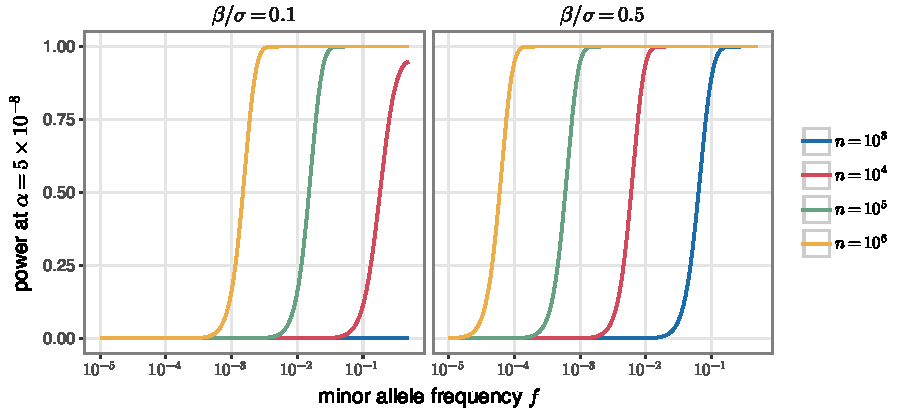
\includegraphics[width=0.9\linewidth]{power_single_variant.pdf}
  \caption{Power of a single-variant additive test at $\alpha=5\times10^{-8}$ as a function of MAF, for sample sizes from $10^3$ to $10^6$ and two standardized effect sizes. Power depends on $N$ and $f$ through approximately $Nf$, so the curves are shifted copies on the log scale. Computed from~\eqref{eq:ncp}.}
  \label{fig:power_single}
\end{figure}

Two strategies follow. Since we cannot test each rare variant on its own, we \emph{aggregate} variants within a unit, usually a gene, and test the unit. And since aggregation dilutes the signal with neutral variants, we use \emph{prior information} to pick out, or upweight, the variants likely to be functional.

%======================================================================
\section{Burden tests}
\label{sec:burden}
%======================================================================

A burden test asks whether a gene carries more variants, or more damaging variants, in affected individuals than expected by chance. Let a gene or region contain $M$ variants that pass some filter, for example $f_j<1\%$ and a predicted loss of function. Let $\mG\in\{0,1,2\}^{N\times M}$ be the genotype matrix, with $G_{ij}$ the number of minor alleles of variant $j$ carried by individual $i$, and let $\vw\in\R^M_{\geq 0}$ be a vector of variant weights. The \emph{burden score} of individual $i$ is
\begin{equation}
  C_i = \sum_{j=1}^M w_j G_{ij} .
\end{equation}
Early versions collapse the variants into an indicator of carrying any qualifying variant, $C_i=\ind[\sum_j G_{ij}>0]$~\citep{morgenthaler2007, li2008}, or weight each variant by $w_j=1/\sqrt{f_j(1-f_j)}$, so that rarer variants count for more~\citep{madsen2009}. The burden score then replaces the genotype in a regression. With covariates $\vx_i\in\R^{C}$ (for example age, sex and genetic principal components), coefficients $\valpha\in\R^C$ and mean $\mu_i=\E[y_i]$,
\begin{equation}
  h(\mu_i) = \vx_i^\top\valpha + C_i\beta ,
  \label{eq:burden_glm}
\end{equation}
where $h$ is the identity for a quantitative trait and the logit for a binary trait. The test of $H_0:\beta=0$ is a single-degree-of-freedom test, so it is as cheap as testing one common variant.

The burden model is the per-variant model $h(\mu_i)=\vx_i^\top\valpha+\sum_j G_{ij}\beta_j$ with the constraint $\beta_j=w_j\beta$. It assumes that every qualifying variant has an effect, in the same direction, of size proportional to its weight. When this holds, pooling the variants concentrates their signal into one statistic. When it does not, the test loses power: neutral variants add noise to $C_i$, and variants with opposite effects cancel.

\subsection{The score test}

The tests in this chapter are \emph{score tests}, which need only the model fitted under the null hypothesis. For a quantitative trait, fit $y_i=\vx_i^\top\valpha+\epsilon_i$ by least squares and let $\hat\mu_i=\vx_i^\top\hat\valpha$ be the fitted values. The score for $\beta$ at $\beta=0$ is the derivative of the log likelihood, $\sigma^{-2}\sum_i C_i(y_i-\hat\mu_i)$. Define the score statistic of variant $j$ as
\begin{equation}
  S_j = \sum_{i=1}^N G_{ij}(y_i-\hat\mu_i), \qquad \vS = \mG^\top(\vy-\hat\vmu)\in\R^M ,
  \label{eq:score}
\end{equation}
so that the burden score is $\sum_i C_i(y_i-\hat\mu_i)=\vw^\top\vS$. Let $\mP_0=\mI-\mX(\mX^\top\mX)^{-1}\mX^\top$ be the $N\times N$ projection onto the residual space of the covariate matrix $\mX\in\R^{N\times C}$. The residuals are $\vy-\hat\vmu=\mP_0\vy$, and under $H_0$ they are distributed as $\Normal(\mathbf{0},\sigma^2\mP_0)$, since $\mP_0$ is symmetric and idempotent. It follows that
\begin{equation}
  \vS\sim\Normal\left(\mathbf{0},\ \sigma^2\mG^\top\mP_0\mG\right), \qquad
  Q_{\text{burden}} = \frac{(\vw^\top\vS)^2}{\hat\sigma^2\,\vw^\top\mG^\top\mP_0\mG\vw} \sim \chi^2_1 .
\end{equation}
For a binary trait fitted by logistic regression the same holds with $\sigma^2\mI$ replaced by $\mV=\operatorname{diag}(\hat\mu_i(1-\hat\mu_i))$ and $\mP_0$ by its weighted version. The vector $\vS$ and its covariance are \emph{summary statistics}: studies can share them without sharing genotypes, and they can be combined across studies by adding them, which makes the tests below suitable for meta-analysis.

\subsection{Counting tests and de novo mutations}

In a case-control study, the simplest burden test counts carriers. Let $a$ of $N_1$ cases and $b$ of $N_0$ controls carry a qualifying variant in the gene. Fisher's exact test on the $2\times 2$ table of carrier status against disease status tests whether the carrier proportions differ.

For de novo mutations the comparison is against a mutation model rather than controls. Sequencing parent-child trios identifies the mutations each child carries that neither parent does. Let $T$ be the number of trios and $\mu_g$ the per-generation probability that a new mutation of a given class (for example protein-truncating) arises in gene $g$ on one haploid genome. Each child receives two haploid genomes, so the expected number of de novo mutations in gene $g$ across the cohort is $\lambda_g=2T\mu_g$, and the number observed, $k_g$, is approximately Poisson distributed under the null hypothesis that the gene plays no role in the disease. The p-value is
\begin{equation}
  P(K\geq k_g) = 1-\sum_{k=0}^{k_g-1}\frac{\lambda_g^k e^{-\lambda_g}}{k!}, \qquad K\sim\Pois(\lambda_g).
\end{equation}
The mutation rate $\mu_g$ must be modelled carefully, because some positions mutate much more often than others. The cytosine of a CpG dinucleotide is usually methylated, and methylated cytosine deaminates spontaneously to thymine, so CG$\to$TG changes occur roughly an order of magnitude more often than other transitions. Gene-level rates are therefore computed by summing per-site probabilities that depend on the sequence context, typically the trinucleotide around each site~\citep{samocha2014}. A gene with many CpGs, or a long gene, is expected to receive more mutations by chance.

\subsection{Practical choices}

A burden analysis involves several choices, each of which can make or break it.
\begin{itemize}
  \item \emph{Which variants qualify.} A MAF threshold (1\%, 0.1\%, singletons only) and a functional filter: protein-truncating variants only, or also missense variants predicted to be damaging, and if so by which predictor (Section~\ref{sec:pathogenicity}). Including more variants adds signal if they are functional and noise if not.
  \item \emph{Missing data.} Sequencing coverage varies across the genome and between samples. A variant can be absent from a sample because it is not there or because the site was not sequenced well enough to call it. If coverage differs between cases and controls, for example because they were sequenced at different centres, the difference alone creates spurious burden.
  \item \emph{Controls.} Sequencing controls is expensive, so it is tempting to compare cases with public databases such as gnomAD~\citep{karczewski2020}, which report allele counts for well over a hundred thousand individuals. TRAPD~\citep{guo2018} does this for exome data: it restricts the comparison to sites that are well covered in both data sets, applies matched quality filters, and calibrates the test using synonymous variants, which should show no excess in cases. Differences in sequencing technology, variant calling and ancestry between cases and public controls remain the main source of false positives.
\end{itemize}

Population data also tell us which genes tolerate damaging variation. For each gene, gnomAD compares the number of protein-truncating (loss-of-function, LoF) variants observed in the population with the number expected under a mutation model like the one above. A gene in which far fewer LoF variants are seen than expected is under strong selection: losing one copy is harmful enough that carriers have fewer children. The upper bound of the confidence interval on the observed/expected ratio (LOEUF) summarizes this constraint~\citep{karczewski2020}. Restricting a burden test to LoF-intolerant genes, or upweighting them, enriches for genes where a new damaging variant is likely to cause disease. We will see this in Section~\ref{sec:autism}.

%======================================================================
\section{Predicting pathogenicity}
\label{sec:pathogenicity}
%======================================================================

Burden tests need to know which variants to include, and every method in this chapter benefits from knowing which variants are likely to be functional. For protein-coding variants we have the genetic code: a premature stop codon or frameshift usually destroys the protein, a missense variant changes one amino acid, and a synonymous variant changes none, although it can still alter splicing (Chapter 10). Most of the genome is noncoding, and there the question of which variants matter is much harder. Pathogenicity predictors fall into a few families.
\begin{itemize}
  \item \emph{Conservation scores} measure how much a position has changed across species. phyloP~\citep{pollard2010} tests each position for slower (or faster) evolution than expected under neutrality on a phylogeny of many species; phastCons~\citep{siepel2005} uses a phylogenetic hidden Markov model (Chapter 6) to find conserved elements; GERP++~\citep{davydov2010} counts ``rejected substitutions''. Conservation is informative but misses functional elements that are specific to humans or primates, and regulatory elements turn over fast in evolution.
  \item \emph{Supervised combinations of annotations.} CADD~\citep{kircher2014} trains a classifier, originally a linear support vector machine, to distinguish variants that became fixed in the human lineage since the human-chimpanzee ancestor, which have survived selection and are mostly benign, from simulated de novo variants, which include deleterious ones in their natural proportion. Its features are many annotations, including conservation, regulatory marks and gene models. FunSeq2~\citep{fu2014} scores noncoding variants by combining conservation, regulatory annotations and network information.
  \item \emph{Unsupervised combinations.} Eigen~\citep{ionitalaza2016} combines many annotations without labelled variants. Its simplest variant, Eigen-PC, scores a variant by the projection of its annotations onto the leading eigenvector of their correlation matrix.
  \item \emph{Sequence models.} Deep learning models such as DeepSEA~\citep{zhou2015} (Chapter 2) predict chromatin features from sequence and so can score the effect of any variant, including variants never seen before, by comparing predictions for the two alleles.
\end{itemize}
A recurring problem is the lack of labels. There are few confirmed pathogenic noncoding variants, and those we have are biased towards particular regions, such as promoters of known disease genes. LINSIGHT avoids labelled variants altogether by learning from the signature that natural selection leaves in population and comparative genomic data.

\subsection{LINSIGHT}

LINSIGHT~\citep{huang2017} combines a generalized linear model of genomic features with INSIGHT, a probabilistic model of molecular evolution~\citep{gronau2013}. Its predecessor fitCons~\citep{gulko2015} grouped sites by their pattern of functional genomic marks and fitted INSIGHT to each group; LINSIGHT replaces the groups with a linear model, which scales to many features and gives a score for each site.

The data are of two kinds (Figure~\ref{fig:linsight_model}). Polymorphism data come from human genomes (54 unrelated individuals in the original study) and record, for each site, whether it is variable in humans and at what frequency. Divergence data come from outgroup primate genomes (chimpanzee, orangutan and rhesus macaque), which, through a phylogenetic model, give the probable ancestral allele and whether the human lineage has acquired a substitution since the ancestor. Natural selection changes both. At a site under purifying selection, new mutations are removed, so we expect fewer substitutions, fewer polymorphisms, and those polymorphisms that exist to be at low frequency, because harmful alleles do not drift to high frequency. A neutral site accumulates substitutions and polymorphisms at the background rate, with the neutral distribution of allele frequencies. The neutral rates vary along the genome with local mutation rate and genealogy, so they are estimated from flanking regions assumed to be neutral.

\begin{figure}[!htbp]
  \centering
  \begin{tikzpicture}[>=Stealth, every node/.style={font=\small},
      lat/.style={circle, draw, minimum size=8mm, inner sep=0pt},
      obs/.style={circle, draw, fill=gray!25, minimum size=8mm, inner sep=0pt},
      det/.style={diamond, draw, aspect=1, inner sep=1.5pt}]
    % outgroup tree
    \node[lat] (r) at (0,3.2) {};
    \node[lat] (n2) at (1.2,2.4) {};
    \node[lat] (Z) at (2.4,1.6) {$Z_i$};
    \node[obs] (o1) at (-0.8,0) {};
    \node[obs] (o2) at (0.6,0) {};
    \node[obs] (o3) at (1.8,0) {};
    \draw[->] (r) -- (o1); \draw[->, dashed] (r) -- (n2); \draw[->] (n2) -- (o2); \draw[->] (Z) -- (o3);
    \draw[->] (n2) -- (Z);
    \node[below=1mm of o2, align=center] {outgroups (primates)};
    \node[lat] (A) at (4.2,1.6) {$A_i$};
    \node[obs] (X) at (4.2,0) {$X_i$};
    \node[below=1mm of X, align=center] {human\\polymorphism};
    \draw[->] (Z) -- node[above] {$\lambda_i$} (A);
    \draw[->] (A) -- node[left, font=\footnotesize] {$\theta_i,\boldsymbol\beta$} (X);
    \node[lat] (Si) at (5.8,2.6) {$S_i$};
    \draw[->] (Si) -- (A); \draw[->] (Si) -- (X);
    \node (rho) at (8.1,2.6) {$\rho_i=g(\vw_\rho^\top\vd_i)$};
    \node (gam) at (8.1,0.3) {$\gamma_i=h(\vw_\gamma^\top\vd_i)$};
    \draw[->] (rho) -- (Si); \draw[->] (gam) -- (X);
    \node[draw, rounded corners, align=left, font=\footnotesize] (feat) at (11.4,1.45) {features $\vd_i$:\\phyloP score\\DNase peak\\TF binding site\\\dots};
    \draw[->] (feat.west) -- (rho.east); \draw[->] (feat.west) -- (gam.east);
  \end{tikzpicture}
  \caption{The LINSIGHT model for site $i$. Grey nodes are observed. Outgroup sequences inform the human-chimpanzee ancestral allele $Z_i$ and, with the neutral divergence rate $\lambda_i$, the human ancestral allele $A_i$. The observed human polymorphism data $X_i$ depend on the neutral polymorphism rate $\theta_i$, the neutral frequency spectrum $\boldsymbol\beta$ and the selection indicator $S_i$. The prior probability of selection $\rho_i$ and the relative rate of low-frequency polymorphism under selection $\gamma_i$ are functions of genomic features $\vd_i$. Redrawn after \citet{huang2017}.}
  \label{fig:linsight_model}
\end{figure}

Table~\ref{tab:linsight} lists the quantities in the model. For site $i$, the binary variable $S_i$ indicates whether the site is under selection, with prior probability $\rho_i$. To see how the likelihood works, assume the ancestral allele is known and classify the human data at site $i$ into five patterns: monomorphic with the ancestral allele ($\mathsf{M}$); monomorphic with a derived allele, that is, a substitution on the human lineage ($\mathsf{D}$); or polymorphic with the derived allele at low ($\mathsf{L}$), intermediate ($\mathsf{I}$) or high ($\mathsf{H}$) frequency. Under neutrality a polymorphism occurs with probability $\theta_i$ and its derived allele frequency falls into the three classes with probabilities $\boldsymbol\beta=(\beta_1,\beta_2,\beta_3)$, and a substitution occurs with probability $\lambda_i$. Under selection, substitutions and intermediate- or high-frequency polymorphisms are not allowed, and low-frequency polymorphisms occur at a rate reduced by the factor $\gamma_i$. This gives
\begin{center}
  \begin{tabular}{lcc}
    \toprule
    pattern $X_i$ & $P(X_i\mid S_i=0)$, neutral & $P(X_i\mid S_i=1)$, selected \\
    \midrule
    $\mathsf{M}$, monomorphic, ancestral & $(1-\theta_i)(1-\lambda_i)$ & $1-\gamma_i\theta_i$ \\
    $\mathsf{D}$, substitution & $(1-\theta_i)\lambda_i$ & $0$ \\
    $\mathsf{L}$, low-frequency derived & $\theta_i\beta_1$ & $\gamma_i\theta_i$ \\
    $\mathsf{I}$, intermediate-frequency derived & $\theta_i\beta_2$ & $0$ \\
    $\mathsf{H}$, high-frequency derived & $\theta_i\beta_3$ & $0$ \\
    \bottomrule
  \end{tabular}
\end{center}
Each column sums to one. INSIGHT also allows adaptive substitutions under selection; LINSIGHT drops this term because positive selection has a negligible effect at the genome-wide scale. The full model integrates over the uncertain ancestral allele with the outgroup phylogeny, and defines frequency classes by a threshold on the minor allele frequency, which complicates the expressions without changing their logic. Marginalizing over $S_i$, the likelihood of site $i$ is
\begin{equation}
  P(X_i) = \rho_i\,P(X_i\mid S_i=1) + (1-\rho_i)\,P(X_i\mid S_i=0) .
  \label{eq:linsight_lik}
\end{equation}

\begin{table}[!htbp]
  \centering
  \caption{Quantities in the LINSIGHT model, after \citet{huang2017}.}
  \label{tab:linsight}
  \begin{tabular}{lp{0.68\linewidth}}
    \toprule
    \multicolumn{2}{l}{\emph{Parameters inherited from INSIGHT}} \\
    $\rho_i$ & probability that site $i$ is under selection; the LINSIGHT score of site $i$ \\
    $\gamma_i$ & expected relative rate of low-frequency derived alleles at site $i$ given that it is under selection \\
    $\lambda_i$ & neutral substitution (divergence) rate at site $i$ \\
    $\theta_i$ & neutral polymorphism rate at site $i$ \\
    $\boldsymbol\beta=(\beta_1,\beta_2,\beta_3)$ & fractions of neutral polymorphisms with low-, intermediate- and high-frequency derived alleles \\
    \midrule
    \multicolumn{2}{l}{\emph{Variables inherited from INSIGHT}} \\
    $X_i$ & observed polymorphism data at site $i$: major allele, minor allele and minor allele frequency class \\
    $Z_i$ & human-chimpanzee ancestral allele at site $i$ \\
    $A_i$ & human ancestral allele at site $i$ \\
    $S_i$ & indicator of whether site $i$ is under selection \\
    \midrule
    \multicolumn{2}{l}{\emph{Components of the generalized linear model}} \\
    $\vd_i\in\R^m$ & genomic feature vector of site $i$ \\
    $\vw_\rho\in\R^m$ & weight vector for $\rho$ (free parameters) \\
    $\vw_\gamma\in\R^m$ & weight vector for $\gamma$ (free parameters) \\
    \bottomrule
  \end{tabular}
\end{table}

A single site carries almost no information: nearly all sites are monomorphic in a sample of a few dozen genomes, whether selected or not. INSIGHT obtained information by pooling many sites of the same type and estimating one $\rho$ for the group. LINSIGHT pools through features instead. Let $\vd_i\in\R^m$ be the feature vector of site $i$, including an intercept; the original model used $m=48$ features in three classes, conservation scores (phyloP, phastCons and others), predicted binding sites (transcription factor and microRNA binding sites, splice sites) and regional annotations (ChIP-seq, DNase-seq and histone modification peaks, enhancer annotations, distance to the nearest transcription start site). The two selection parameters are
\begin{equation}
  \rho_i = g(\vw_\rho^\top\vd_i), \qquad \gamma_i = h(\vw_\gamma^\top\vd_i),
\end{equation}
with weight vectors $\vw_\rho,\vw_\gamma\in\R^m$. The link $h$ is the logistic function. For $g$, LINSIGHT uses the asymmetric Gompertz function $g(x)=\exp(-3e^{-x})$, which, unlike the logistic, keeps the gradient from vanishing when $\rho_i$ is close to zero, as it is at most sites. The neutral parameters $\lambda_i$, $\theta_i$ and $\boldsymbol\beta$ are estimated beforehand from the flanking neutral regions and held fixed. The weights maximize the log likelihood $\sum_i\log P(X_i)$ over all noncoding sites in the genome, billions of terms, which is done by stochastic gradient ascent on minibatches of sites (Chapter 2). The model is a generalized linear model whose ``response'' $X_i$ is linked to the linear predictor through the mixture~\eqref{eq:linsight_lik} rather than through a standard exponential family.

The LINSIGHT score of a site is $\rho_i$, the \emph{prior} probability of selection given its features, not the posterior $P(S_i=1\mid X_i)$. This is deliberate: the score of a site should not depend on whether a polymorphism happens to have been observed there in 54 genomes, and the prior is defined for every site, including those where a patient carries a variant never seen before. Because $\rho_i$ is a probability that a mutation at site $i$ is selected against, it is also called the \emph{fitness consequence} of the site. Figure~\ref{fig:linsight_fitness}a shows that it behaves as expected across annotation classes: low for intergenic and intronic sites, higher for UTRs, promoters and binding sites, and highest at splice sites.

\begin{figure}[!htbp]
  \centering
  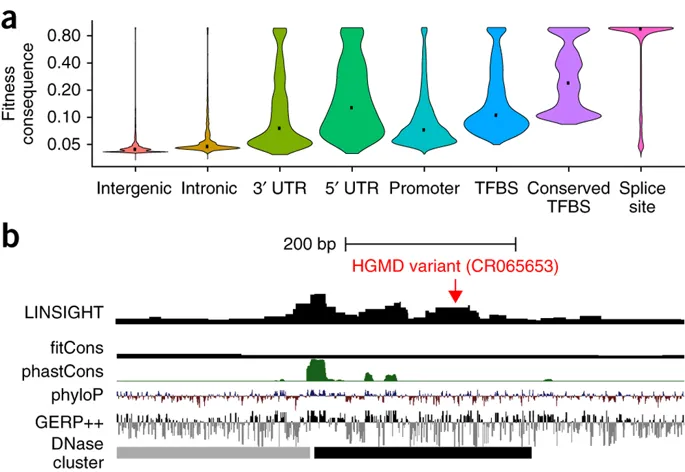
\includegraphics[width=0.75\linewidth]{slides/linsight_fitness.png}
  \caption{(a) Distribution of LINSIGHT scores (fitness consequence, log scale) of noncoding sites in different annotation classes. TFBS, transcription factor binding site. (b) LINSIGHT and other scores around a noncoding disease variant from the Human Gene Mutation Database. LINSIGHT is elevated across the DNase hypersensitive region containing the variant, whereas the conservation scores (phastCons, phyloP, GERP++) give little signal at the variant itself. Reproduced from \citet{huang2017}.}
  \label{fig:linsight_fitness}
\end{figure}

\subsection{Evaluating pathogenicity scores}

To evaluate a predictor we need variants of known effect. \citet{huang2017} used noncoding variants from the Human Gene Mutation Database (HGMD), which catalogues variants reported to cause inherited disease, and from ClinVar, as positives, and common SNPs (MAF $>1\%$) as negatives. The ROC curves (Chapter 1) in Figure~\ref{fig:linsight_roc} show LINSIGHT ahead of the alternatives, with phyloP, which uses conservation alone, the weakest. Two caveats apply to this kind of benchmark. Common variants are an easy negative set, since a variant that has risen to high frequency is unlikely to be strongly deleterious, so the task differs from the clinical one of distinguishing a pathogenic rare variant from a benign rare variant. The authors therefore also used negatives matched to the positives by distance to the transcription start site, or drawn from within 1 kb of each disease variant. And the positives are biased toward regions people have looked at, such as promoters of known disease genes, so methods that learn ``near a known disease gene'' are rewarded.

\begin{figure}[!htbp]
  \centering
  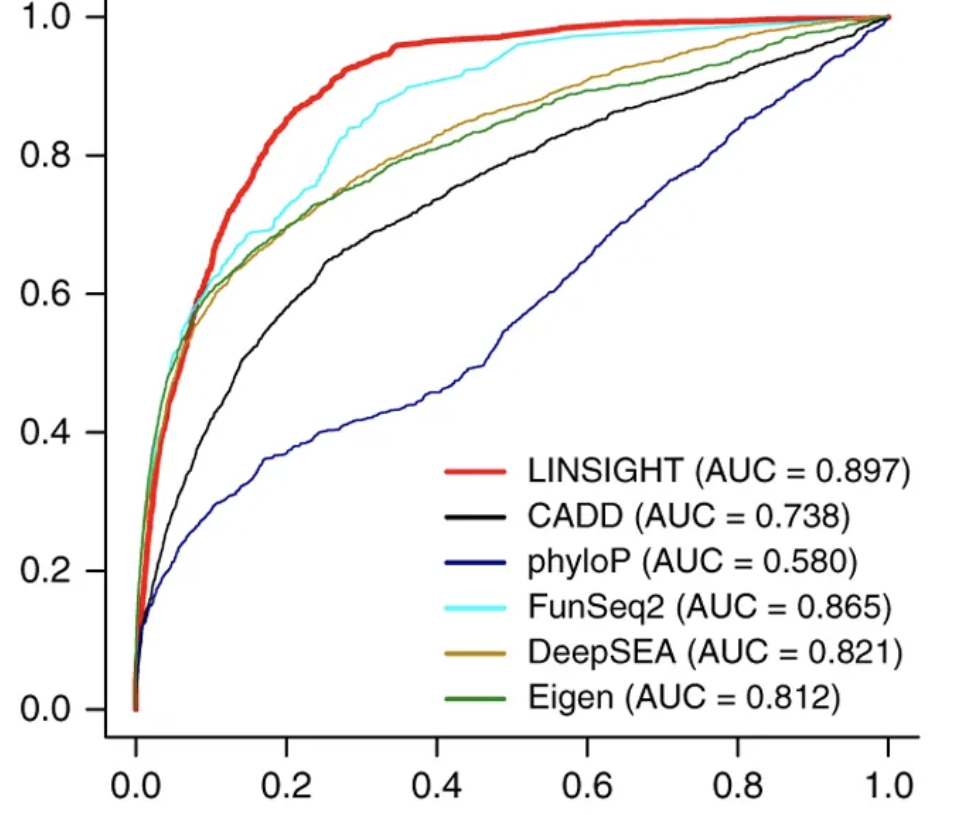
\includegraphics[width=0.5\linewidth]{slides/linsight_hgmd_roc.png}
  \caption{ROC curves (true positive rate against false positive rate) for distinguishing noncoding disease variants from HGMD from common SNPs not matched to the disease variants by location. phyloP, conservation across species; CADD, a classifier of observed against simulated variants; FunSeq2 and DeepSEA, see text; Eigen, an unsupervised combination of annotations. Reproduced from \citet{huang2017}.}
  \label{fig:linsight_roc}
\end{figure}

%======================================================================
\section{Variance component tests: SKAT and SKAT-O}
\label{sec:skat}
%======================================================================

Burden tests assume that all qualifying variants act in the same direction. This is reasonable for loss-of-function variants in a gene where losing one copy is harmful, but not in general. Some missense variants increase protein activity and others decrease it; in a regulatory region some variants increase expression and others decrease it; and most variants in a region may be neutral. The sequence kernel association test (SKAT)~\citep{wu2011} drops the assumption by treating the per-variant effects as random with mean zero, and SKAT-O~\citep{lee2012} interpolates between SKAT and the burden test.

\subsection{The model}

Let $\vg_i\in\{0,1,2\}^M$ be the genotypes of individual $i$ at the $M$ variants, so that $\vg_i^\top$ is row $i$ of $\mG$. The per-variant model is
\begin{equation}
  h(\mu_i) = \vx_i^\top\valpha + \vg_i^\top\vb, \qquad \vb\in\R^M,
\end{equation}
with $\vb$ random and
\begin{equation}
  \E[\beta_j]=0, \qquad \Var(\beta_j)=w_j^2\tau, \qquad \Cov(\beta_{j_1},\beta_{j_2})=\rho\,w_{j_1}w_{j_2}\tau \quad (j_1\neq j_2),
  \label{eq:skat_prior}
\end{equation}
where $\tau\geq 0$ is a variance component, $w_j$ is the weight of variant $j$ and $\rho\in[0,1]$ is the correlation between effects. In matrix form, $\Cov(\vb)=\tau\mW\mR_\rho\mW$, with $\mW=\operatorname{diag}(\vw)$ and $\mR_\rho=(1-\rho)\mI_M+\rho\ind\ind^\top$, where $\ind$ is the vector of $M$ ones. Two cases are of interest. With $\rho=0$ the effects are independent, with random signs and magnitudes that scale with $w_j$; this is SKAT, also called a \emph{dispersion} test, because it detects effects that spread the trait in either direction. With $\rho=1$ the effects are perfectly correlated, so $\vb=\vw\beta_0$ for a single random $\beta_0$ with variance $\tau$, which is the burden model~\eqref{eq:burden_glm}. The null hypothesis $\vb=\mathbf{0}$ becomes $H_0:\tau=0$, a test of one parameter however many variants the region contains.

\subsection{Deriving the score statistic}

For a quantitative trait with Gaussian noise, take $\vb$ to be Gaussian as well. Then $\vb$ can be integrated out, as for ridge regression in Chapter 1, and
\begin{equation}
  \vy\sim\Normal\left(\mX\valpha,\ \mSigma(\tau)\right), \qquad \mSigma(\tau) = \sigma^2\mI_N + \tau\mK, \qquad \mK = \mG\mW\mR_\rho\mW\mG^\top ,
\end{equation}
where $\mK\in\R^{N\times N}$ is a kernel matrix: $K_{ii'}$ measures the weighted genetic similarity of individuals $i$ and $i'$ in the region. Let $\vr=\vy-\mX\valpha$. The log likelihood is $\ell(\tau)=-\frac{1}{2}\log|\mSigma(\tau)|-\frac{1}{2}\vr^\top\mSigma(\tau)^{-1}\vr+\text{const}$. Using $\partial\log|\mSigma|/\partial\tau=\tr(\mSigma^{-1}\partial\mSigma/\partial\tau)$ and $\partial\mSigma^{-1}/\partial\tau=-\mSigma^{-1}(\partial\mSigma/\partial\tau)\mSigma^{-1}$, with $\partial\mSigma/\partial\tau=\mK$,
\begin{equation}
  \frac{\partial\ell}{\partial\tau} = -\frac{1}{2}\tr\left(\mSigma^{-1}\mK\right) + \frac{1}{2}\vr^\top\mSigma^{-1}\mK\mSigma^{-1}\vr .
\end{equation}
At $\tau=0$, $\mSigma=\sigma^2\mI$ and
\begin{equation}
  \left.\frac{\partial\ell}{\partial\tau}\right|_{\tau=0} = \frac{1}{2\sigma^4}\vr^\top\mK\vr - \frac{1}{2\sigma^2}\tr(\mK) .
\end{equation}
The trace term does not depend on the data, so the test can be based on the quadratic form in the residuals $\hat\vr=\vy-\mX\hat\valpha$ from the null model. Substituting $\mK$ and the score vector $\vS=\mG^\top\hat\vr$ from~\eqref{eq:score},
\begin{equation}
  Q_\rho = \hat\vr^\top\mK\hat\vr = \vS^\top\mW\mR_\rho\mW\vS
  = (1-\rho)\underbrace{\sum_{j=1}^M w_j^2S_j^2}_{Q_{\text{SKAT}}} + \rho\underbrace{\Big(\sum_{j=1}^M w_jS_j\Big)^2}_{Q_{\text{burden}}} .
  \label{eq:skat_q}
\end{equation}
The SKAT statistic is a weighted sum of the squared single-variant score statistics, and the burden statistic is the square of their weighted sum. The difference explains when each works. Under the alternative, $\E[S_j]$ has the sign of $\beta_j$ (for variants in weak linkage disequilibrium). Squaring before summing makes $Q_{\text{SKAT}}$ insensitive to the signs, while in $Q_{\text{burden}}$ variants with opposite effects cancel. Conversely, when all effects share a sign, $Q_{\text{burden}}$ adds their signals coherently while $Q_{\text{SKAT}}$ also accumulates noise from the squared scores of neutral variants. For binary traits the same argument applied to a logistic mixed model gives a score statistic of the same form~\eqref{eq:skat_q}, with residuals $y_i-\hat\mu_i$ from the null logistic regression~\citep{wu2011}.

The SKAT framework allows any positive semi-definite kernel in place of $\mG\mW\mW\mG^\top$, for example kernels based on the number of alleles two people share identical by state, which can capture interactions between variants~\citep{wu2011}. The weighted linear kernel is the one used in practice.

\subsection{The null distribution}

Under $H_0$, $\vS\sim\Normal(\mathbf{0},\sigma^2\boldsymbol{\Omega})$ with $\boldsymbol{\Omega}=\mG^\top\mP_0\mG\in\R^{M\times M}$, as shown in Section~\ref{sec:burden}. Write $\vS=\sigma\boldsymbol{\Omega}^{1/2}\vz$ with $\vz\sim\Normal(\mathbf{0},\mI_M)$ and let $\mathbf{A}_\rho=\mW\mR_\rho\mW$. Then
\begin{equation}
  \frac{Q_\rho}{\sigma^2} = \vz^\top\boldsymbol{\Omega}^{1/2}\mathbf{A}_\rho\boldsymbol{\Omega}^{1/2}\vz = \sum_{k=1}^M \lambda_k u_k^2, \qquad u_k\overset{\text{iid}}{\sim}\Normal(0,1),
\end{equation}
where $\lambda_1,\dots,\lambda_M\geq 0$ are the eigenvalues of $\boldsymbol{\Omega}^{1/2}\mathbf{A}_\rho\boldsymbol{\Omega}^{1/2}$ and the second equality follows by rotating $\vz$ into its eigenbasis. The null distribution of $Q_\rho/\sigma^2$ is therefore a weighted sum of independent $\chi^2_1$ variables. Its tail probability has no closed form but can be computed by numerically inverting the characteristic function~\citep{davies1980} or approximated by matching moments to a scaled $\chi^2$~\citep{liu2009}. In practice $\sigma^2$ is replaced by its estimate under the null. For burden ($\rho=1$) the matrix $\mathbf{A}_1=\vw\vw^\top$ has rank one, a single eigenvalue $\lambda_1=\vw^\top\boldsymbol{\Omega}\vw$ is non-zero, and we recover the $\chi^2_1$ test of Section~\ref{sec:burden}.

\subsection{Variant weights}

The default SKAT weights are the $\BetaD(1,25)$ density evaluated at the MAF, $w_j=25(1-f_j)^{24}$ (Figure~\ref{fig:maf_weights}). The weight is nearly constant for $f_j$ below about 0.005 and falls to almost zero by $f_j=0.1$, so rare variants dominate the statistic, which encodes the expectation from Figure~\ref{fig:effect_freq} that rarer variants have larger effects. Under~\eqref{eq:skat_prior} the expected contribution of variant $j$ to the trait variance is $2f_j(1-f_j)w_j^2\tau$, so the choice of weights is a prior on how variance explained is spread across the frequency spectrum. The weights are also the natural place to put functional information, a point we return to in Section~\ref{sec:fst}.

\begin{figure}[!htbp]
  \centering
  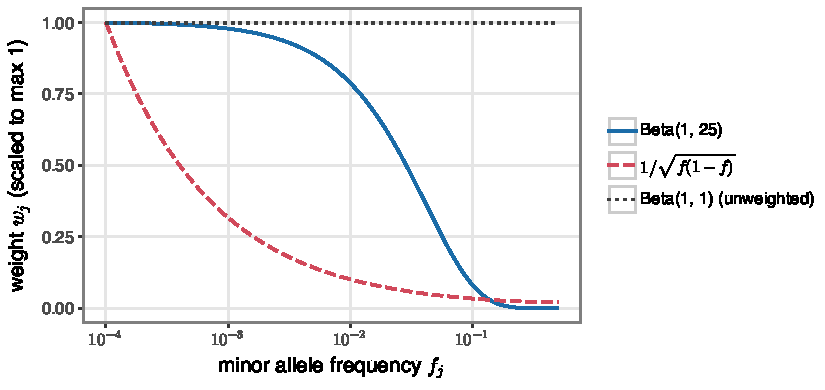
\includegraphics[width=0.8\linewidth]{maf_weights.pdf}
  \caption{Variant weights as a function of MAF, each scaled to a maximum of one: the $\BetaD(1,25)$ density used by default in SKAT, the Madsen-Browning weight $1/\sqrt{f(1-f)}$, and equal weights.}
  \label{fig:maf_weights}
\end{figure}

\subsection{SKAT-O}

We rarely know in advance whether a gene's variants act in one direction. SKAT-O~\citep{lee2012} computes $Q_\rho$ over a grid $0=\rho_1<\rho_2<\dots<\rho_B=1$, for example $\rho\in\{0,0.1^2,0.2^2,0.3^2,0.4^2,0.5^2,1\}$, and uses the smallest p-value,
\begin{equation}
  T = \min_{b=1,\dots,B} p_{\rho_b},
\end{equation}
where $p_{\rho_b}$ is the p-value of $Q_{\rho_b}$. $T$ is not itself a p-value, because taking the minimum over several tests makes small values more likely. Its null distribution follows from the joint distribution of the $Q_\rho$, which are all quadratic forms in the same $\vS$. Because $Q_\rho$ is linear in $\rho$, it is a combination of $Q_{\text{SKAT}}$ and $Q_{\text{burden}}$, and \citet{lee2012} decompose it into a $\chi^2_1$ part and an approximately independent remainder, which reduces the p-value of $T$ to a one-dimensional numerical integral. They also give a small-sample correction for binary traits, where the asymptotic null distribution can be poor.

Why not estimate $\rho$, for example by maximum likelihood, and plug it in? Under $H_0$, $\tau=0$ and $\rho$ has no effect on the likelihood: it is not identifiable. A parameter that exists only under the alternative breaks the usual asymptotic theory for likelihood ratio and score tests, so the plug-in statistic has no standard null distribution. Taking the minimum p-value over a grid and computing the exact null distribution of the minimum sidesteps the problem. The price is a modest loss of power relative to knowing the best $\rho$ in advance.

\subsection{Comparing the tests}

Figure~\ref{fig:skat_power} compares the three tests in a simulated region of 39 rare variants. When most variants are causal and all increase the trait, the burden test is the most powerful. When few variants are causal, or when effects have mixed signs, SKAT is much more powerful, and with mixed signs the burden test has almost no power at all. SKAT-O is close to the better of the two in every setting. It is never the best by much, but it is never far from the best, which is why it is a common default.

\begin{figure}[!htbp]
  \centering
  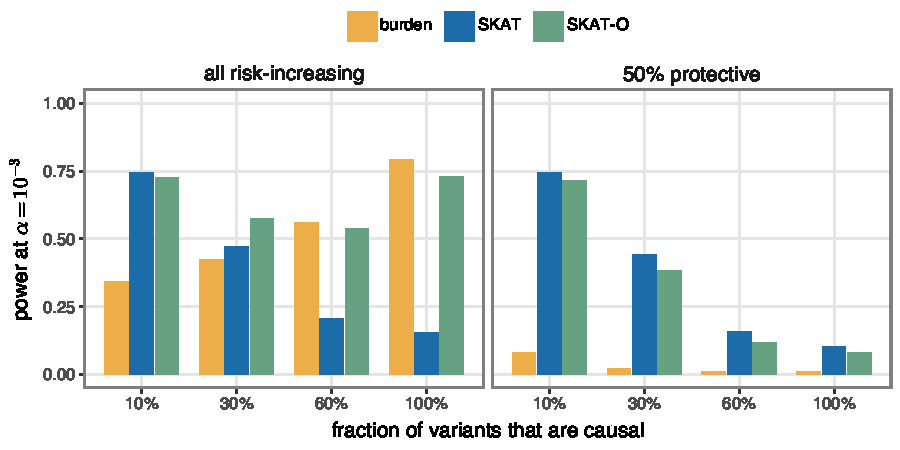
\includegraphics[width=0.9\linewidth]{skat_power.pdf}
  \caption{Power of burden, SKAT and SKAT-O tests (with $\BetaD(1,25)$ weights) in a simulated region of $M=39$ independent variants with MAF between 0.0005 and 0.02, for a quantitative trait in $N=2000$ individuals. Each variant is causal with the probability on the horizontal axis and has effect $|\beta_j|=a|\log_{10}f_j|$, with the sign either always positive (left) or random (right). The scale $a$ is smaller for larger causal fractions, so power should be compared between tests within a group of bars, not across groups. Null distributions were computed by simulating $2\times10^5$ score vectors for the fixed genotype matrix; 1000 replicates per setting.}
  \label{fig:skat_power}
\end{figure}

%======================================================================
\section{Using functional annotations in the test}
\label{sec:fst}
%======================================================================

A pathogenicity score such as LINSIGHT, CADD or Eigen gives, for each variant, an estimate of how likely it is to be functional. There are two simple ways to use it in a set-based test: filter variants on a threshold, as in a burden analysis, or multiply the MAF weights by the score, $w_j\to w_jZ_j$, where $Z_j\geq 0$ is the score of variant $j$. Both help if the score predicts which variants affect the trait and hurt if it does not. For noncoding variants, where scores are weak and a score built for one purpose (say, conservation) may not predict effects on a particular trait, this matters. \citet{he2017} proposed tests that use several annotations at once and lose little power when an annotation is uninformative. We call this the functional score test (FST).

\subsection{The model}

Let $q$ be the number of annotations and $Z_{jk}$ the $k$-th functional score of variant $j$, $k=1,\dots,q$. The effect of variant $j$ is decomposed as
\begin{equation}
  \beta_j = \gamma_{j0} + \sum_{k=1}^q Z_{jk}\gamma_{jk} ,
\end{equation}
where each $\gamma_{jk}$ is random with mean zero, $\Var(\gamma_{jk})=w_j^2\tau_k$ and $\Cov(\gamma_{j_1k},\gamma_{j_2k})=\rho\,w_{j_1}w_{j_2}\tau_k$, and the $\gamma_{j0},\dots,\gamma_{jq}$ are independent for each $j$. The variance component $\tau_k\geq 0$ measures how much of the genetic effect in the region tracks annotation $k$, and $\tau_0$ the part that tracks no annotation. Then
\begin{align}
  \Var(\beta_j) &= w_j^2\Big(\tau_0+\sum_{k=1}^q Z_{jk}^2\tau_k\Big), \\
  \Cov(\beta_{j_1},\beta_{j_2}) &= \rho\,w_{j_1}w_{j_2}\Big(\tau_0+\sum_{k=1}^q Z_{j_1k}Z_{j_2k}\tau_k\Big).
\end{align}
Setting $Z_{j0}=1$ and $\mD_k=\operatorname{diag}(w_1Z_{1k},\dots,w_MZ_{Mk})$, the covariance of $\vb$ is a sum of SKAT-O covariances, one per annotation,
\begin{equation}
  \Cov(\vb) = \sum_{k=0}^q \tau_k\,\mD_k\mR_\rho\mD_k ,
\end{equation}
and the null hypothesis of no association is $H_0:\tau_0=\tau_1=\dots=\tau_q=0$.

\subsection{The test}

Repeating the derivation of Section~\ref{sec:skat} for each $\tau_k$ in turn gives one score statistic per annotation,
\begin{equation}
  Q_{\rho,k} = \vS^\top\mD_k\mR_\rho\mD_k\vS = (1-\rho)\sum_{j=1}^M w_j^2Z_{jk}^2S_j^2 + \rho\Big(\sum_{j=1}^M w_jZ_{jk}S_j\Big)^2 ,
\end{equation}
which is the SKAT-O statistic with weights $w_jZ_{jk}$. $Q_{\rho,0}$ is the original test with MAF weights only. \citet{he2017} combine these statistics by their minimum p-value, $T=\min_{k,\rho}p_{\rho,k}$, over $k=0,\dots,q$ and, in practice, $\rho\in\{0,1\}$, so that the combined test takes the best of the dispersion and burden tests for each annotation. The null distribution of $T$ is obtained from the null distribution of $\vS$ alone. Score vectors are drawn from $\Normal(\mathbf{0},\hat\sigma^2\boldsymbol{\Omega})$, each $p_{\rho,k}$ is computed by moment matching, and the vector of normal scores $\boldsymbol\delta$ with elements $\Phi^{-1}(p_{\rho,k})$ is approximated as multivariate normal with the correlation matrix estimated from the draws. The p-value of an observed $T=t$ is then $1-P(\delta_{\rho,k}>\Phi^{-1}(t)\text{ for all }k,\rho)$, a multivariate normal probability. Only $\vS$ and $\boldsymbol{\Omega}$ are needed, so the test works with summary statistics and, by adding them across studies, in meta-analysis.

The construction has a simple logic. The unified test always contains the original test, $k=0$, so when the annotations are uninformative it loses only what the multiple-testing correction across the $2(q+1)$ statistics costs. When an annotation is informative, the corresponding reweighted statistic carries the signal.

\subsection{Power}

\citet{he2017} simulated regions in which 10\% of variants were causal and annotation $k$ predicted the causal variants with probability $P_k$. They compared the original tests with $\BetaD(1,25)$ weights (O), tests with weights multiplied by the first score (W1), and unified tests with the first score (U1) or the first two scores (U1+2). When neither score was informative ($P_1=P_2=0$), W1 lost a large fraction of the power of O while U1 and U1+2 lost none, and could even gain slightly. When the first score was informative, W1, U1 and U1+2 all improved on O. When only the second score was informative, U1+2 was the most powerful and W1 the least. The pattern held for dispersion, burden and combined tests.

Figure~\ref{fig:fst_power} reproduces the logic in a small simulation of our own, using a region simulated as in Figure~\ref{fig:skat_power} and a single annotation. With an uninformative score, reweighting (W) costs most of the power, while the unified test (U) stays close to the original (O). With an informative score, reweighting helps the burden test a great deal, because it removes the neutral variants that dilute the burden, and the unified test captures most of the gain. SKAT gains less from the annotation, since squaring the scores already lets the variants with large $S_j$ dominate.

\begin{figure}[!htbp]
  \centering
  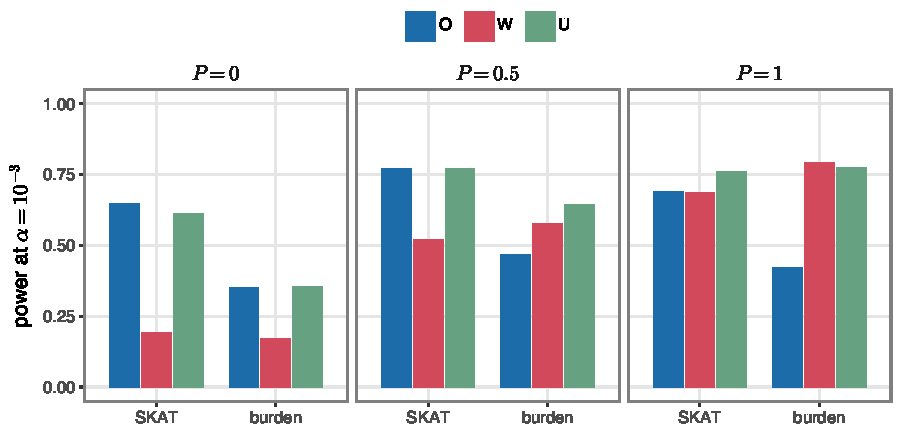
\includegraphics[width=0.9\linewidth]{fst_power.pdf}
  \caption{Power of SKAT and burden tests with $\BetaD(1,25)$ weights (O), weights multiplied by a functional score (W), and the unified minimum p-value test over both weightings (U). In a region simulated as in Figure~\ref{fig:skat_power}, 20\% of variants are causal with positive effects $\beta_j=0.28|\log_{10}f_j|$. The score is $\chi^2_1$ for non-causal variants; for each causal variant it is non-central $\chi^2_1$ (non-centrality 4) with probability $P$ and $\chi^2_1$ otherwise. 50 draws of the causal set and scores, 20 trait replicates each, $\alpha=10^{-3}$. Within a panel the tests are applied to the same simulated traits.}
  \label{fig:fst_power}
\end{figure}

%======================================================================
\section{Case study: noncoding de novo mutations in autism}
\label{sec:autism}
%======================================================================

Autism spectrum disorder (ASD) has a substantial contribution from de novo mutations. Exome sequencing of families found that children with ASD carry more de novo protein-truncating mutations than their unaffected siblings~\citep{iossifov2014}, and burden tests of such mutations have identified many ASD genes. In Chapter 10 we saw that de novo mutations predicted by SpliceAI to disrupt splicing are also enriched in ASD and intellectual disability. Most de novo mutations, about 70 per genome, fall outside coding sequence, and whether noncoding de novo mutations contribute was an open question. Noncoding mutations cannot be tested one at a time, and there is no simple equivalent of ``protein-truncating'' to define which ones to aggregate. \citet{zhou2019} used deep learning sequence models to supply that definition.

\subsection{Data and design}

The data were whole genomes from 1,790 \emph{simplex} families from the Simons Simplex Collection, 7,097 genomes in total. A simplex family has exactly one affected child, the proband, together with unaffected parents and, in most families, an unaffected sibling (Figure~\ref{fig:asd_pipeline}). Simplex families are enriched for de novo causes, because an inherited cause of large effect would often have affected other family members. The unaffected siblings are a natural control group. They have the same parents, so their expected de novo mutation rate is similar, and their genomes were sequenced and processed in the same way as the probands', so technical artefacts in mutation calling affect both groups alike. The comparison is therefore between the de novo mutations of probands and those of siblings, and the question is whether the probands' mutations are more damaging.

\subsection{Scoring mutations}

Each de novo mutation was scored with two DeepSEA-style convolutional networks (Chapter 2), which take 1,000 bp of sequence centred on the variant and predict the probability of each of many chromatin or RNA-binding features. The transcriptional regulation model predicts 2,002 features (DNase hypersensitivity, transcription factor binding and histone marks) and was trained on ENCODE and Roadmap Epigenomics profiles. The post-transcriptional model predicts 232 features, mostly RNA-binding protein (RBP) binding sites measured by CLIP-seq, which captures the sites on RNA bound by a given protein. For each mutation and feature $\ell$, the variant effect is the absolute difference between the predictions for the two alleles, $|p_\ell(\text{alt})-p_\ell(\text{ref})|$.

These thousands of predicted effects must be reduced to one number per mutation, the probability that it is harmful. \citet{zhou2019} trained a regularized logistic regression (Chapter 1) with the standardized predicted effects as features, separately for transcriptional and post-transcriptional effects. Positive examples were 4,401 noncoding regulatory mutations reported in HGMD to cause disease. Negative examples were 999,668 \emph{singleton} variants observed in healthy individuals in the 1000 Genomes Project. Singletons are a better negative set than common variants because they are rare, like de novo mutations, and so have similar sequence context and mutational processes; they are mostly benign, but selection has had little time to remove the damaging ones, so the negative set is somewhat contaminated. Classes were weighted inversely to their size to counter the imbalance. The predicted probabilities were standardized across all proband and sibling mutations to give a \emph{disease impact score} (DIS) for each mutation. The classifier never sees autism data: it learns what Mendelian disease mutations look like through the eyes of the sequence models, and is then applied to a different disease.

\begin{figure}[!htbp]
  \centering
  \begin{tikzpicture}[>=Stealth, every node/.style={font=\small},
      box/.style={draw, rounded corners, align=center, inner sep=4pt}]
    % pedigree
    \node[draw, minimum size=8mm] (fa) at (0,2.2) {};
    \node[draw, circle, minimum size=8mm] (mo) at (2.0,2.2) {};
    \node[above=1pt of fa, font=\footnotesize] {father};
    \node[above=1pt of mo, font=\footnotesize] {mother};
    \draw (fa.east) -- (mo.west);
    \draw (1.0,2.2) -- (1.0,1.5) -- (0,1.5) -- (0,1.1);
    \draw (1.0,1.5) -- (2.0,1.5) -- (2.0,1.1);
    \node[draw, diamond, fill=black, minimum size=9mm, inner sep=0pt] (pr) at (0,0.7) {};
    \node[draw, diamond, minimum size=9mm, inner sep=0pt] (sb) at (2.0,0.7) {};
    \node[below=1pt of pr, font=\footnotesize] {proband};
    \node[below=1pt of sb, font=\footnotesize] {sibling};
    \node[align=center, font=\footnotesize] at (1.0,-0.6) {1,790 simplex families\\7,097 genomes};
    % pipeline
    \begin{scope}[box/.append style={text width=6.2cm, font=\footnotesize}]
    \node[box] (seq) at (7.0,2.9) {1,000 bp around each de novo mutation (reference and alternative allele)};
    \node[box, below=4mm of seq] (cnn) {DeepSEA models: 2,002 transcriptional and 232 post-transcriptional features};
    \node[box, below=4mm of cnn] (lr) {regularized logistic regression on $|\Delta p|$: HGMD (4,401) vs singletons (999,668)};
    \node[box, below=4mm of lr] (dis) {disease impact score per mutation};
    \end{scope}
    \node[box, text width=2.3cm, font=\footnotesize] (cmp) at (12.2,-0.9) {proband vs sibling: rank-sum test};
    \node[box, text width=2.3cm, font=\footnotesize] (nd) at (12.2,0.7) {network enrichment (NDEA)};
    \draw[->] (seq) -- (cnn); \draw[->] (cnn) -- (lr); \draw[->] (lr) -- (dis);
    \draw[->] (dis) -- (cmp); \draw[->] (dis.east) -- ++(0.4,0) |- (nd.west);
    \draw[->, dashed] (2.6,0.7) -- (3.6,0.7) node[midway, above, font=\footnotesize] {DNMs};
  \end{tikzpicture}
  \caption{Design of the autism noncoding mutation study. Each simplex family has one affected child (proband, filled) and an unaffected sibling. De novo mutations (DNMs) are scored by sequence models, the predicted effects are combined into a disease impact score by a classifier trained on known disease mutations, and the scores of proband and sibling mutations are compared. After \citet{zhou2019}.}
  \label{fig:asd_pipeline}
\end{figure}

\subsection{Comparing probands and siblings}

The scores of proband and sibling mutations were compared with a one-sided Wilcoxon rank-sum (Mann-Whitney) test. Let $d^P_1,\dots,d^P_{n_P}$ be the DIS values of proband mutations and $d^S_1,\dots,d^S_{n_S}$ those of sibling mutations. Rank all $n_P+n_S$ values together, let $R_P$ be the sum of the ranks of the proband mutations, and define $U=R_P-n_P(n_P+1)/2$, the number of (proband, sibling) pairs in which the proband mutation has the higher score. Under the null hypothesis that the two groups have the same distribution, and with no ties,
\begin{equation}
  \E[U]=\frac{n_Pn_S}{2}, \qquad \Var(U)=\frac{n_Pn_S(n_P+n_S+1)}{12},
\end{equation}
and $(U-\E[U])/\sqrt{\Var(U)}$ is approximately standard normal for large samples. The test uses only ranks, so it is robust to the heavy tail of the score distribution, in which a few mutations have very high predicted impact. The quantity $U/(n_Pn_S)$ is the probability that a random proband mutation scores higher than a random sibling mutation, the same quantity as the AUROC of Chapter 1.

Proband mutations had significantly higher disease impact scores than sibling mutations, for both transcriptional and post-transcriptional effects (Figure~\ref{fig:asd_dis}). The difference was larger for mutations near genes, and larger again near genes that are intolerant of loss-of-function variation in the population. The effect is small on average, as expected if only a minority of probands carry a causal noncoding mutation.

\begin{figure}[!htbp]
  \centering
  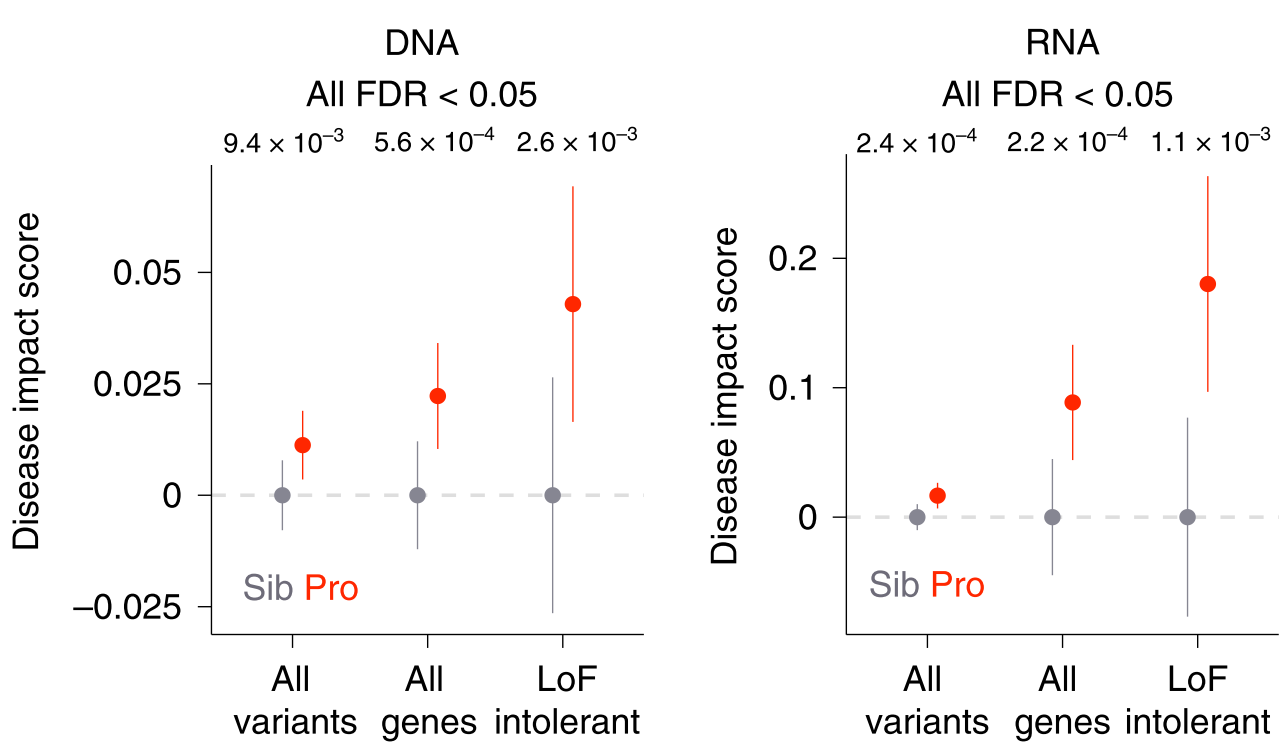
\includegraphics[width=0.7\linewidth]{slides/asd_disease_impact.png}
  \caption{Mean disease impact score of de novo mutations in probands (red) and unaffected siblings (grey), for predicted transcriptional (DNA) and post-transcriptional (RNA) effects. Scores are normalized by subtracting the sibling mean, so siblings are at zero; bars show 95\% confidence intervals. Mutations are shown for all variants, variants assigned to any gene, and variants assigned to genes intolerant of loss of function, with the significance of each comparison above; all comparisons have false discovery rate below 0.05. Reproduced from \citet{zhou2019}.}
  \label{fig:asd_dis}
\end{figure}

%======================================================================
\section{Network differential enrichment analysis}
\label{sec:ndea}
%======================================================================

Even with a good score, de novo mutations are too sparse to implicate individual genes: most genes receive no mutation in either group, and few receive more than one. \citet{zhou2019} therefore borrowed strength across genes using a gene network. The network was the brain-specific functional network of \citet{greene2015}, one of a set of tissue-specific networks built by Bayesian integration of thousands of genome-scale data sets (expression, protein interactions, and others) against tissue-specific gold standards. Unlike the co-expression and partial-correlation networks of Chapter 9, its edges are not estimated from one data type: the weight $A_{uv}\in[0,1]$ is the posterior probability that genes $u$ and $v$ act together in brain.

Network differential enrichment analysis (NDEA) asks, for each gene $u$, whether the mutations in genes functionally connected to $u$ have higher scores in probands than in siblings. Let $\mathcal{P}$ and $\mathcal{S}$ be the sets of proband and sibling mutations, $d_m$ the disease impact score of mutation $m$, and $v(m)$ the gene to which it is assigned (the nearest gene within a distance threshold). Each mutation receives a weight for gene $u$,
\begin{equation}
  a_{um} = \frac{A_{u,v(m)}}{n_{v(m)}} ,
\end{equation}
where $n_{v}$ is the number of mutations in the same group (proband or sibling) assigned to gene $v$, so that a gene with many mutations does not dominate. The weighted mean scores of the two groups are
\begin{equation}
  \mu_{\mathcal{P}}(u) = \frac{\sum_{m\in\mathcal{P}}a_{um}d_m}{\sum_{m\in\mathcal{P}}a_{um}}, \qquad
  \mu_{\mathcal{S}}(u) = \frac{\sum_{m\in\mathcal{S}}a_{um}d_m}{\sum_{m\in\mathcal{S}}a_{um}} ,
\end{equation}
and they are compared with a weighted version of Welch's $t$ statistic,
\begin{equation}
  t_u = \frac{\mu_{\mathcal{P}}(u)-\mu_{\mathcal{S}}(u)}{\sqrt{V_{\mathcal{P}}(u)/N_{\mathcal{P}}(u)+V_{\mathcal{S}}(u)/N_{\mathcal{S}}(u)}} .
  \label{eq:ndea}
\end{equation}
Here, for group $\mathcal{G}\in\{\mathcal{P},\mathcal{S}\}$, dropping the dependence on $u$,
\begin{equation}
  V_{\mathcal{G}} = \frac{\sum_{m\in\mathcal{G}}a_{m}(d_m-\mu_{\mathcal{G}})^2}{\sum_{m\in\mathcal{G}}a_m-\sum_{m\in\mathcal{G}}a_m^2\big/\sum_{m\in\mathcal{G}}a_m}, \qquad
  N_{\mathcal{G}} = \frac{\left(\sum_{m\in\mathcal{G}}a_m\right)^2}{\sum_{m\in\mathcal{G}}a_m^2} .
\end{equation}
Both quantities generalize their unweighted counterparts. Suppose the $d_m$ in a group are independent with mean $\mu$ and variance $v$, and the weights are fixed. Writing $A_1=\sum_m a_m$ and $A_2=\sum_m a_m^2$, the weighted mean $\hat\mu=\sum_m a_md_m/A_1$ has variance
\begin{equation}
  \Var(\hat\mu) = \frac{\sum_m a_m^2 v}{A_1^2} = \frac{v}{N}, \qquad N=\frac{A_1^2}{A_2},
\end{equation}
so $N$ is the \emph{effective sample size}: the number of equally weighted observations that would give the same variance. It equals the number of mutations when the weights are equal, and is smaller when a few mutations carry most of the weight. For the variance, $\sum_ma_m(d_m-\hat\mu)^2=\sum_ma_md_m^2-A_1\hat\mu^2$, with $\E[\sum_ma_md_m^2]=A_1(v+\mu^2)$ and $\E[\hat\mu^2]=\mu^2+vA_2/A_1^2$, so
\begin{equation}
  \E\Big[\sum_ma_m(d_m-\hat\mu)^2\Big] = A_1(v+\mu^2) - A_1\mu^2 - v\frac{A_2}{A_1} = v\left(A_1-\frac{A_2}{A_1}\right),
\end{equation}
and $V$ is an unbiased estimate of $v$. With equal weights $a_m=1$ in a group of $n$ mutations, $A_1=n$, $A_2=n$, $N=n$ and $V=\sum_m(d_m-\hat\mu)^2/(n-1)$, the usual sample variance, so~\eqref{eq:ndea} reduces to Welch's $t$. The statistic is compared with a $t$ distribution whose degrees of freedom follow from the Welch-Satterthwaite approximation with $N_{\mathcal{P}}$ and $N_{\mathcal{S}}$ in place of the group sizes.

A gene can score highly without carrying a single mutation, if its network neighbours carry high-impact proband mutations (Figure~\ref{fig:ndea}). The same test applies to a gene set, such as a Gene Ontology (GO) term, by treating the set as one node whose edge weight to gene $v$ is the average of $A_{u v}$ over the genes $u$ in the set. Among the terms enriched at false discovery rate below 0.05 were many neuronal functions: regulation of synapse assembly, axon guidance, dendrite development, the synaptic vesicle cycle, postsynaptic density and neuron migration. Clustering the top-ranked genes on the network gave groups related to synaptic function and to chromatin regulation. Both themes had already emerged from coding de novo mutations in ASD: genes for synaptic function, which are specific to neurons, and genes for transcriptional and chromatin regulation, which act in every cell type yet seem to matter most for neurodevelopment. The noncoding mutations point to the same biology.

\begin{figure}[!htbp]
  \centering
  \begin{tikzpicture}[>=Stealth, every node/.style={font=\small},
      gene/.style={circle, draw, minimum size=8mm, inner sep=0pt, fill=blue!10}]
    \node[gene, fill=orange!30, minimum size=10mm] (u) at (0,0) {$u$};
    \node[gene] (v1) at (-2.6,1.2) {$v_1$};
    \node[gene] (v2) at (-2.4,-1.4) {$v_2$};
    \node[gene] (v3) at (2.6,1.0) {$v_3$};
    \node[gene] (v4) at (2.8,-1.2) {$v_4$};
    \draw[line width=2.2pt, gray] (u) -- node[above, black, font=\footnotesize] {0.9} (v1);
    \draw[line width=1.6pt, gray] (u) -- node[below, black, font=\footnotesize] {0.6} (v2);
    \draw[line width=0.6pt, gray] (u) -- node[above, black, font=\footnotesize] {0.1} (v3);
    \draw[line width=1.2pt, gray] (u) -- node[below, black, font=\footnotesize] {0.4} (v4);
    \foreach \n/\c/\dx/\dy in {v1/red/-0.8/0.5, v1/red/-0.9/-0.1, v2/red/-0.9/-0.3, v2/gray/-0.5/-0.8, v3/gray/0.9/0.4, v4/red/0.9/-0.5, v4/gray/0.6/-0.9} {
      \draw[\c!80!black] (\n) -- ++(\dx,\dy) node[star, star points=5, fill=\c!70, draw=\c!80!black, inner sep=1.2pt] {};
    }
    \node[align=left, font=\footnotesize] at (6.3,0.3) {\textcolor{red!70!black}{$\star$} proband mutation\\\textcolor{gray}{$\star$} sibling mutation\\edge: $A_{uv}$};
  \end{tikzpicture}
  \caption{Network differential enrichment analysis for gene $u$. Mutations assigned to other genes $v$ are weighted by the network edge weight $A_{uv}$, and the weighted mean disease impact scores of proband and sibling mutations are compared with a weighted $t$ test. Gene $u$ can be implicated without carrying a mutation itself.}
  \label{fig:ndea}
\end{figure}

%======================================================================
\section{Experimental validation}
\label{sec:validation}
%======================================================================

Statistical enrichment shows that proband mutations as a group have higher predicted impact, not that any particular mutation does anything. \citet{zhou2019} tested prioritized mutations with \emph{luciferase reporter assays}. For each selected proband mutation with predicted transcriptional effect (positive disease impact score, near a gene with prior evidence for a role in ASD), 230 bp of sequence around the mutation was cloned, once with the de novo allele and once with the reference allele carried by the sibling, upstream of a minimal promoter driving the firefly luciferase gene. The constructs were transfected into a human neuroblastoma cell line, and the light produced, normalized to a co-transfected control reporter and to the empty vector, measures how strongly each sequence drives transcription. Of 59 tested regions that showed transcriptional activity, 57 showed a significant difference between the two alleles (Figure~\ref{fig:luciferase}). A predicted splicing-disrupting mutation was tested in a similar way with a minigene, a reporter containing the exon and flanking introns, and reduced inclusion of the exon.

\begin{figure}[!htbp]
  \centering
  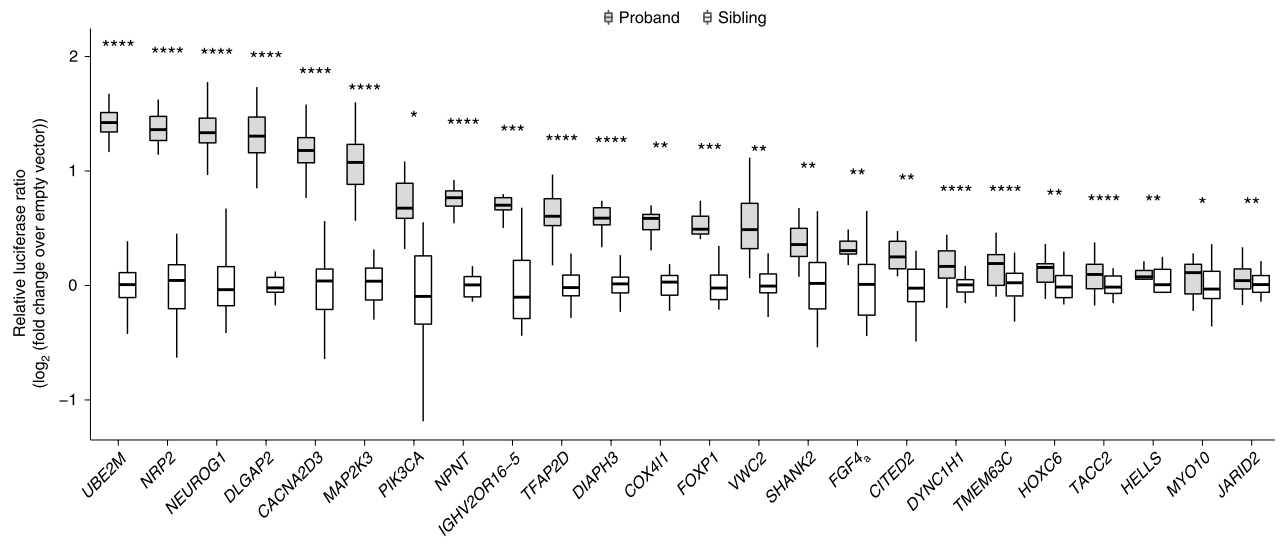
\includegraphics[width=\linewidth]{slides/asd_luciferase.png}
  \caption{Luciferase reporter activity (log$_2$ fold change over empty vector) of sequences carrying the proband's de novo allele (grey) or the reference allele carried by the sibling (white), for prioritized mutations near the genes shown. Asterisks mark significant differences between alleles. Reproduced from \citet{zhou2019}.}
  \label{fig:luciferase}
\end{figure}

Reporter assays have clear limits. The sequence is tested outside its chromosomal context, on a plasmid, in one cell line that may not express the relevant transcription factors, and without the gene it normally regulates. A difference between alleles shows that the mutation changes regulatory activity, not that the change affects the target gene in the developing brain, let alone that it contributes to ASD. Massively parallel reporter assays apply the same idea to thousands of sequences at once, and genome editing of the endogenous locus gives stronger evidence at much greater cost.

%======================================================================
\section{Using molecular data from patients}
\label{sec:molecular}
%======================================================================

So far the evidence that a rare variant matters has come from prediction or from aggregating many individuals. For a patient with a suspected Mendelian disease, the question is narrower: which of the patient's rare variants, if any, causes the disease? Exome or genome sequencing finds a causal variant in only a minority of patients, often because the culprit is noncoding or its effect is not recognizable from sequence. RNA-seq from the patient, increasingly obtained alongside whole-genome sequencing in clinical genetics, can show the consequence of a variant directly. A variant that disrupts a promoter or enhancer lowers the expression of the haplotype that carries it (Figure~\ref{fig:reg_variant}); one that disrupts a splice site produces aberrant isoforms; one that creates a premature stop codon triggers nonsense-mediated decay of the transcript. Each leaves a trace in RNA-seq, and the task is to recognize a trace that is unusual relative to the population. The tissue matters: the relevant gene must be expressed in the sample, which is why blood, skin fibroblasts and, for muscle diseases, muscle biopsies are used.

\begin{figure}[!htbp]
  \centering
  \begin{tikzpicture}[>=Stealth, every node/.style={font=\small}]
    \node[font=\ttfamily\footnotesize, anchor=west] (s1) at (0,0.25) {AGTACCAGTCGATGTTTACGTACCGTACGATCGAATCGATCCATCGAATT};
    \node[font=\ttfamily\footnotesize, anchor=west] (s2) at (0,-0.25) {AGTACCAGTCGATGTTTACGTACCG\textcolor{red}{C}ACGATCGAATCGATCCATCGAATT};
    \draw[thick] (0,0.75) -- (12.8,0.75);
    \draw[thick] (0,-0.75) -- (12.8,-0.75);
    \fill (9.2,0.6) rectangle (12.4,0.9); \node[white, font=\footnotesize\itshape] at (10.8,0.75) {GENE ABC};
    \fill (9.2,-0.9) rectangle (12.4,-0.6); \node[white, font=\footnotesize\itshape] at (10.8,-0.75) {GENE ABC};
    \draw[line width=2.5pt, -{Stealth[length=3mm]}] (9.2,0.9) -- (9.2,1.35) -- (10.2,1.35);
    \draw[line width=0.6pt, -{Stealth[length=1.5mm]}] (9.2,-0.9) -- (9.2,-1.2) -- (9.8,-1.2);
    \node[right, font=\footnotesize] at (0,1.05) {haplotype 1: high expression};
    \node[right, font=\footnotesize] at (0,-1.05) {haplotype 2: rare regulatory variant, low expression};
  \end{tikzpicture}
  \caption{A rare variant (red) in a regulatory element upstream of a gene reduces transcription from the haplotype that carries it. In RNA-seq this appears as reduced total expression and as allelic imbalance at heterozygous sites in the gene.}
  \label{fig:reg_variant}
\end{figure}

\subsection{Expression and splicing outliers}

An \emph{expression outlier} is a gene whose expression in the patient is extreme relative to a reference population, such as the GTEx samples of the same tissue. After normalizing expression and removing the effects of known covariates and hidden confounders (Chapter 12), the expression of gene $u$ in the patient is converted to a $z$-score, $z_u=(e_u-\bar e_u)/s_u$, with $\bar e_u$ and $s_u$ the mean and standard deviation of the normalized expression $e_u$ across the reference samples (Figure~\ref{fig:outliers}a). In GTEx, individuals who were expression outliers for a gene, particularly consistently across tissues, were enriched for rare variants near that gene, with the strongest enrichment for structural variants, frameshifts and splice-site variants~\citep{li2017}. Combining expression, splicing and allelic outlier signals with variant annotations improves the prioritization further~\citep{ferraro2020}.

A \emph{splicing outlier} is an aberrant splicing event: a splice junction that is used in the patient but rarely or never in controls, or a change in the relative usage of junctions (Figure~\ref{fig:outliers}b). Splicing quantification was the subject of Chapter 10. \citet{cummings2017} applied RNA-seq of muscle biopsies to patients with rare muscle disorders who remained undiagnosed after exome or genome sequencing, and found pathogenic exon skipping, exon extension and splice-site creation events absent from GTEx muscle samples, which established a diagnosis for a substantial fraction of the patients. Several of the causal variants were deep intronic or exonic changes whose effect on splicing had not been recognized from sequence.

\begin{figure}[!htbp]
  \centering
  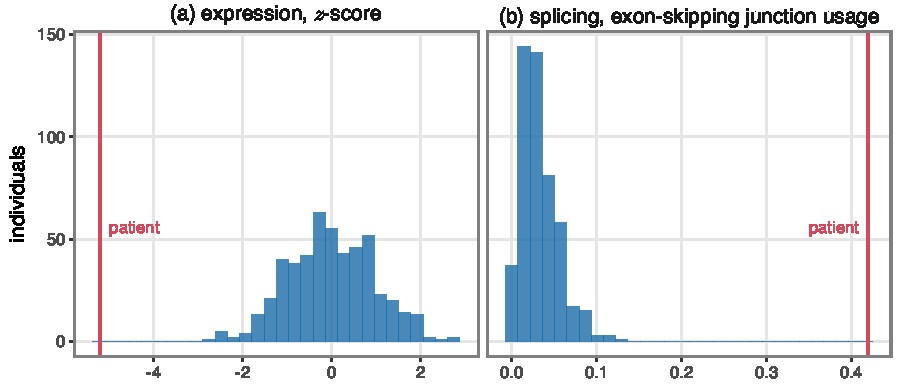
\includegraphics[width=0.95\linewidth]{outliers.pdf}
  \caption{Outlier detection against a reference population of 500 simulated individuals. (a) Expression $z$-scores of one gene; the patient (red) has $z=-5.2$. (b) Fraction of reads at an exon that use a junction skipping it; the patient uses the skipping junction in 42\% of reads, against a few percent in the reference population.}
  \label{fig:outliers}
\end{figure}

\subsection{Allelic outliers}

Allele-specific expression (ASE), introduced in Chapter 12, gives a test within the patient: at a heterozygous site in a transcribed region, the reads from the two haplotypes can be counted, and an imbalance means that one haplotype is expressed more than the other. A rare regulatory variant or a nonsense-mediated decay trigger on one haplotype produces exactly this. The difficulty is that allelic imbalance is common. Most genes have common eQTLs, and in any individual, the two haplotypes of a gene often differ in expression for reasons unrelated to disease. A raw test of imbalance against $1/2$ flags thousands of genes per person.

ANEVA-DOT~\citep{mohammadi2019} addresses this by asking whether the imbalance is unusual \emph{for that gene}. Genes differ in how much regulatory variation the population tolerates. For a dosage-sensitive gene, selection keeps regulatory variants rare and their effects small, so the genetic variance of its expression is low; for a tolerant gene, large common eQTL effects are normal. ANEVA estimates this genetic variance, $V^G$, for each gene from ASE data in a reference population (GTEx). ANEVA-DOT then tests a patient's allelic counts against the distribution implied by $V^G$.

A simplified version of the model is as follows. Let $s\in\R$ be the log$_2$ ratio of the expression of haplotype 1 to haplotype 2 in an individual, the allelic fold change. In the population, $s\sim\Normal(0,V^G)$. Given $s$, a read comes from haplotype 1 with probability $\pi(s)=2^s/(1+2^s)$, and with $n$ reads at the site, the count $r$ from haplotype 1 is beta-binomial (Chapter 12), which allows for overdispersion from technical sources such as PCR duplicates,
\begin{equation}
  r\mid s \sim \operatorname{BetaBinomial}\big(n,\ c\,\pi(s),\ c\,(1-\pi(s))\big),
\end{equation}
where $c>0$ is a concentration parameter. Integrating over $s$ gives the null distribution of $r$ for a patient whose regulatory variation is typical of the population,
\begin{equation}
  P(r\mid n) = \int \Normal(s\mid 0, V^G)\,P(r\mid n,s)\,ds ,
\end{equation}
and the two-sided p-value of the observed count $r_{\text{obs}}$ is $2\min\{P(r\leq r_{\text{obs}}\mid n),P(r\geq r_{\text{obs}}\mid n)\}$. Figure~\ref{fig:aneva_dot} shows the same patient counts, 640 reads from one haplotype and 157 from the other, a four-fold imbalance, against two genes. For a gene with low $V^G$ the imbalance is far outside the population distribution ($p\approx 10^{-12}$); for a gene with high $V^G$ it is unremarkable ($p\approx 0.07$). The scale of what counts as an outlier is set by the population, gene by gene.

\begin{figure}[!htbp]
  \centering
  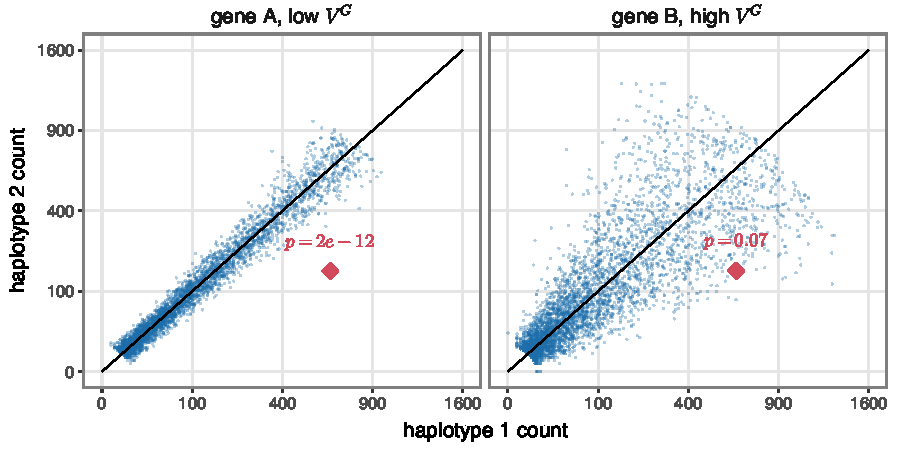
\includegraphics[width=0.9\linewidth]{aneva_dot.pdf}
  \caption{Allelic counts at a heterozygous site for 4000 simulated individuals (blue) drawn from the population model with low ($V^G=0.02$, left) and high ($V^G=1.2$, right) genetic variance of allelic fold change, total counts between 10 and 1600 and beta-binomial concentration $c=200$. Axes are on a square-root scale; the diagonal is allelic balance. The patient (red) has 640 and 157 reads from the two haplotypes; the p-values are from the marginal beta-binomial model. After the ANEVA-DOT analysis of \citet{mohammadi2019}.}
  \label{fig:aneva_dot}
\end{figure}

%======================================================================
\section{Learning gene impairment scores: DeepRVAT}
\label{sec:deeprvat}
%======================================================================

Every test in this chapter needs a rule for turning an individual's variants in a gene into evidence: which variants to include, how to weight them by frequency, and which annotations to trust. Burden tests and SKAT fix the rule in advance. The functional score test picks among a few candidate rules. DeepRVAT~\citep{clarke2024} learns the rule from data with a neural network, shared across genes and traits.

\subsection{A set function of variants}

Let $\mathcal{V}_{iu}$ be the set of rare variants that individual $i$ carries in gene $u$, and $\va_k\in\R^D$ the annotation vector of variant $k$. DeepRVAT used $D=34$ annotations: a transform of the MAF, predicted consequences (missense, stop gain, splice region and so on), protein-level scores (SIFT, PolyPhen-2, AlphaMissense, PrimateAI), CADD and ConDel, splicing predictions (SpliceAI, AbSplice), principal components of DeepSEA chromatin predictions, and predicted RNA-binding protein binding. The \emph{gene impairment score} of individual $i$ in gene $u$ is
\begin{equation}
  \psi(\mathcal{V}_{iu}) = \operatorname{logit}^{-1}\Big(\kappa\Big(\max_{k\in\mathcal{V}_{iu}}\phi(\va_k)\Big)\Big) \in (0,1),
  \label{eq:deeprvat}
\end{equation}
where $\phi:\R^D\to\R^H$ is a multilayer perceptron applied to each variant, the maximum is taken elementwise over the variants in the set, $\kappa:\R^H\to\R$ is a second multilayer perceptron, and $\operatorname{logit}^{-1}$ is the logistic function. (\citet{clarke2024} write $\rho$ for $\kappa$ and $f$ for the pooling operation.) The score is close to one if the gene is likely impaired and close to zero if the variants look benign.

Equation~\eqref{eq:deeprvat} is a \emph{deep set} architecture~\citep{zaheer2017}. The input is a set, with no natural order and variable size, so the function must be invariant to permutations of the variants. \citet{zaheer2017} showed that permutation-invariant functions of sets can be written as $\kappa(\sum_k\phi(\va_k))$ for suitable $\phi$ and $\kappa$; replacing the sum by an elementwise maximum keeps the invariance. The maximum has a natural interpretation here: one damaging variant is enough to impair a gene, and adding benign variants should not increase the score, which a sum would do. Each hidden unit of $\phi$ acts as a learned detector for one kind of damaging variant, and the maximum records whether any variant in the set triggers it.

\begin{figure}[!htbp]
  \centering
  \begin{tikzpicture}[>=Stealth, every node/.style={font=\small},
      box/.style={draw, rounded corners, align=center, inner sep=3pt, minimum height=7mm}]
    \foreach \k/\y in {1/1.2, 2/0, 3/-1.2} {
      \node (a\k) at (0,\y) {$\va_{k_\k}$};
      \node[box, fill=blue!10] (p\k) at (1.8,\y) {$\phi$};
      \draw[->] (a\k) -- (p\k);
    }
    \node[box, fill=orange!20] (mx) at (3.8,0) {elementwise\\max};
    \foreach \k in {1,2,3} \draw[->] (p\k.east) -- (mx.west);
    \node[box, fill=blue!10] (rh) at (5.6,0) {$\kappa$};
    \node[box] (sg) at (7.3,0) {$\operatorname{logit}^{-1}$};
    \node (psi) at (9.1,0) {$\psi(\mathcal{V}_{iu})$};
    \draw[->] (mx) -- (rh); \draw[->] (rh) -- (sg); \draw[->] (sg) -- (psi);
    \node[box] (lin) at (7.6,-1.9) {$\vx_i^\top\valpha^{(p)}+\sum_{u\in\mathcal{S}^{(p)}}w_u^{(p)}\psi(\mathcal{V}_{iu})$};
    \draw[->] (psi) -- (psi |- lin.north);
    \node[right=2mm of lin] {$=\hat y_i^{(p)}$, trait $p$};
    \draw[decorate, decoration={brace, amplitude=4pt}] (-0.4,-1.65) -- (-0.4,1.65) node[midway, left=5pt, align=right] {variants of\\individual $i$\\in gene $u$};
  \end{tikzpicture}
  \caption{DeepRVAT. Each variant's annotations pass through a shared network $\phi$, the outputs are pooled by an elementwise maximum, and a second network $\kappa$ with a logistic output gives the gene impairment score $\psi$. During training, the scores of seed genes predict each trait through a linear model. After \citet{clarke2024}.}
  \label{fig:deeprvat}
\end{figure}

\subsection{Training and testing}

The score function is trained to predict traits. For trait $p$, with covariates $\vx_i$ (age, sex, genetic principal components) and coefficients $\valpha^{(p)}$, the prediction is
\begin{equation}
  \hat y_i^{(p)} = \vx_i^\top\valpha^{(p)} + \sum_{u\in\mathcal{S}^{(p)}} w_u^{(p)}\,\psi(\mathcal{V}_{iu}),
\end{equation}
where $\mathcal{S}^{(p)}$ is a set of \emph{seed genes} for trait $p$ and $w_u^{(p)}\in\R$ is a gene-specific coefficient. The networks $\phi$ and $\kappa$ are shared across all genes and all traits; only $\valpha^{(p)}$ and $w_u^{(p)}$ are specific to a trait. The loss is the squared error averaged over traits, minimized by stochastic gradient descent. The seed genes give the training signal. They were the genes significant in a conventional analysis that combines burden and SKAT tests of loss-of-function and missense variants with $\BetaD(1,25)$ weights. Training used 21 quantitative traits in about 160,000 exome-sequenced individuals from the UK Biobank. Sharing $\psi$ across traits means that what is learned about damaging variants from, say, lipid genes transfers to every other gene and trait. The score is ``trait-agnostic'', a learned, general-purpose definition of gene impairment.

For association testing, the trained $\psi$ is computed for every gene and individual and used as the burden score of Section~\ref{sec:burden}: for each gene $u$, the trait is regressed on $\psi(\mathcal{V}_{iu})$ and the covariates, and $H_0:\beta=0$ is tested with a score test. Genes outside the seed set can therefore be discovered. To avoid circularity, the model is trained with cross-validation: each individual's score is computed from models that were not trained on that individual. The seed genes themselves were chosen using the full data, so \citet{clarke2024} also checked the discoveries by replication in a larger UK Biobank release and on traits not used in training. Compared with burden and SKAT baselines, DeepRVAT found more significant gene-trait associations across the quantitative and binary traits it was applied to, and its scores improved the identification of individuals at high genetic risk.

DeepRVAT illustrates the trajectory of this chapter. A burden test hard-codes the prior that rare damaging variants matter; SKAT and the functional score test let the data choose among a few such priors; DeepRVAT learns the prior as a flexible function of annotations, with the statistical test kept simple so that its calibration is easy to check.

%======================================================================
\section{Summary}
%======================================================================

\begin{itemize}
  \item The power of a single-variant test depends on the sample size and MAF through approximately $Nf$, so rare variants need very large samples and de novo mutations cannot be tested individually. Rare variants can still have large effects, because selection keeps damaging variants rare.
  \item Burden tests aggregate the variants in a gene into a single score. They are powerful when most qualifying variants are causal with effects in the same direction, and depend on choices of frequency threshold, functional filter, controls and quality control. De novo mutations are tested against a mutation-rate model that accounts for sequence context such as CpG sites.
  \item Pathogenicity predictors include conservation scores, supervised and unsupervised combinations of annotations, and sequence models. LINSIGHT learns from the patterns of divergence and polymorphism that natural selection produces, with the prior probability of selection modelled as a function of genomic features.
  \item SKAT treats per-variant effects as random with mean zero and tests their variance component with a score statistic $\sum_jw_j^2S_j^2$ whose null distribution is a mixture of $\chi^2_1$ variables. It is robust to mixed effect directions. SKAT-O combines SKAT and burden through a correlation parameter $\rho$ and the minimum p-value over a grid.
  \item The functional score test adds one variance component per annotation and combines the resulting statistics, gaining power when annotations are informative and losing little when they are not.
  \item In autism, de novo noncoding mutations scored with deep learning sequence models and a classifier trained on known disease mutations have higher predicted impact in probands than in siblings. Network differential enrichment pools sparse mutations across functionally related genes, implicating synaptic and chromatin regulation genes. Reporter assays confirm that prioritized mutations alter regulatory activity.
  \item RNA-seq from patients reveals the consequences of rare variants as expression, splicing or allelic outliers, judged against a reference population, and ANEVA-DOT calibrates allelic imbalance by each gene's tolerance of regulatory variation.
  \item DeepRVAT learns a gene impairment score from variant annotations with a deep set network trained across traits, and uses it as the burden score in a conventional test.
\end{itemize}

%======================================================================
\section*{Exercises}
%======================================================================

\begin{enumerate}
  \item Using~\eqref{eq:ncp}, find the sample size needed for 80\% power at $\alpha=5\times10^{-8}$ to detect a variant with $f=10^{-3}$ and $\beta=0.25\sigma$. How does the answer change if the variant is ten times rarer?
  \item Starting from the marginal likelihood $\vy\sim\Normal(\mX\valpha,\sigma^2\mI+\tau\mG\mW\mR_\rho\mW\mG^\top)$, derive the score statistic~\eqref{eq:skat_q} and show that it equals $(1-\rho)Q_{\text{SKAT}}+\rho Q_{\text{burden}}$.
  \item Suppose a region has $M$ independent variants with equal weights and equal frequencies, half with effect $+\beta$ and half with effect $-\beta$. Show that the expected burden score statistic $\E[\vw^\top\vS]$ is zero under the alternative, while $\E[Q_{\text{SKAT}}]$ increases with $\beta^2$.
  \item For the simplified LINSIGHT likelihood~\eqref{eq:linsight_lik}, derive the gradient of $\log P(X_i)$ with respect to $\vw_\rho$, for the Gompertz link $g(x)=\exp(-3e^{-x})$. Show that sites with the pattern $\mathsf{D}$ always push $\rho_i$ down, and explain why monomorphic sites push it up only slightly.
  \item Show that the effective sample size $N=(\sum_ma_m)^2/\sum_ma_m^2$ satisfies $1\leq N\leq n$ for $n$ positive weights, with equality at the upper end only when all weights are equal.
  \item In the ANEVA-DOT model, show that without overdispersion ($c\to\infty$) and with $V^G\to 0$, the test reduces to a binomial test of $r$ against $n/2$. Why does this test flag far too many genes in practice?
  \item Explain why the elementwise maximum in~\eqref{eq:deeprvat} makes $\psi$ invariant to the order of the variants. Construct an example in which replacing the maximum by a sum would make a gene with many benign variants look more impaired than a gene with one damaging variant.
\end{enumerate}

\bibliographystyle{abbrvnat}
\bibliography{../chapter13/chapter13}
\endgroup

% Generated wrapper: chapter 14 with its own figure path, macros and bibliography.
\graphicspath{{../chapter14/figures/}}
\makeatletter\def\input@path{{../chapter14/}}\makeatother
\begingroup
% Chapter 14: protein structure prediction with AlphaFold 2.
% Requires: amsmath, amssymb, bm, graphicx, booktabs, multirow, subcaption, algorithm, algpseudocode,
% tikz (arrows.meta, positioning, calc, decorations.pathreplacing, decorations.pathmorphing, shapes.geometric, fit), natbib.
% Computed figures are produced by scripts/make_figures.py; figures/slides/ holds figures taken from the lecture slides.

\providecommand{\R}{\mathbb{R}}
\providecommand{\E}{\mathbb{E}}
\providecommand{\Normal}{\mathcal{N}}
\providecommand{\argmax}{\operatorname*{arg\,max}}
\providecommand{\argmin}{\operatorname*{arg\,min}}
\providecommand{\vy}{\mathbf{y}}
\providecommand{\vx}{\mathbf{x}}
\providecommand{\mX}{\mathbf{X}}
\providecommand{\mI}{\mathbf{I}}
\providecommand{\vb}{\boldsymbol{\beta}}
\providecommand{\veps}{\boldsymbol{\epsilon}}
\providecommand{\vp}{\mathbf{p}}
\providecommand{\vg}{\mathbf{g}}
\providecommand{\ind}{\mathbf{1}}
\providecommand{\vh}{\mathbf{h}}
\providecommand{\vq}{\mathbf{q}}
\providecommand{\vk}{\mathbf{k}}
\providecommand{\vv}{\mathbf{v}}
\providecommand{\vz}{\mathbf{z}}
\providecommand{\ve}{\mathbf{e}}
\providecommand{\va}{\mathbf{a}}
\providecommand{\vs}{\mathbf{s}}
\providecommand{\mW}{\mathbf{W}}
\providecommand{\mR}{\mathbf{R}}
\providecommand{\softmax}{\operatorname{softmax}}
\providecommand{\vm}{\mathbf{m}}
\providecommand{\vo}{\mathbf{o}}
\providecommand{\vt}{\mathbf{t}}
\providecommand{\vu}{\mathbf{u}}
\providecommand{\vw}{\mathbf{w}}
\providecommand{\vc}{\mathbf{c}}
\providecommand{\vf}{\mathbf{f}}
\providecommand{\mF}{\mathbf{F}}
\providecommand{\mM}{\mathbf{M}}
\providecommand{\mJ}{\mathbf{J}}
\providecommand{\SE}{\mathrm{SE}(3)}
\providecommand{\SO}{\mathrm{SO}(3)}
\providecommand{\LN}{\operatorname{LN}}
\providecommand{\sigm}{\operatorname{sigmoid}}
\providecommand{\Ca}{C$\alpha$}

\providecommand{\chaptertoc}{}
\chapter{Protein structure prediction with AlphaFold~2}
\label{ch:alphafold}
\chaptertoc

A protein is a chain of amino acids that folds into a three-dimensional shape, and that shape determines what the protein does. Measuring the shape experimentally takes months or years per protein, while sequencing gives us the amino acid sequences of millions of proteins cheaply. Predicting structure from sequence has therefore been a central problem of computational biology for half a century. AlphaFold~2~\citep{jumper2021} solved a large part of this problem in 2020, predicting the structures of many proteins with an accuracy close to that of experiment. It has had a large influence on the interface of machine learning and biology, and its main ideas recur in later models.

AlphaFold~2 combines ideas we have met in earlier chapters, attention and transformers (Chapter 3) and representation learning from large data sets, with ideas specific to proteins. This chapter covers four of these. The first is \emph{evolutionary information}: related proteins in other species, lined up in a multiple sequence alignment, reveal which positions of a protein are in contact. The second is the \emph{Evoformer}, a transformer that operates on two coupled representations, one of the alignment and one of pairs of residues, and that is built to respect the geometry of distances. The third is the \emph{structure module}, which places each residue in space as a rigid body and is designed so that its predictions rotate and translate with the protein. The fourth is the training objective, in particular a loss that compares structures without first superimposing them, and the model's prediction of its own confidence. The presentation follows \citet{jumper2021} and the expository account of \citet{bouatta2021}; the supplementary information of \citet{jumper2021} gives every layer in pseudocode.

%======================================================================
\section{Proteins and the structure prediction problem}
\label{sec:proteins}
%======================================================================

\subsection{Amino acids, the backbone and side chains}

Chapter 1 introduced the central dogma: DNA is transcribed to RNA, which is translated into protein. Translation reads the RNA three nucleotides (one codon) at a time and appends one of 20 amino acids for each codon, so a protein is a linear polymer, a sequence over an alphabet of 20 letters. In the context of a protein, each amino acid is called a \emph{residue}. Typical proteins are a few hundred residues long.

Every amino acid shares the same core of atoms: a nitrogen (N), a central carbon called the alpha carbon (\Ca) and a carbonyl carbon (C, sometimes written C$'$) bonded to an oxygen. Consecutive residues are joined by a \emph{peptide bond} between the carbonyl carbon of one residue and the nitrogen of the next. The repeating chain N--\Ca--C--N--\Ca--C--$\cdots$ is the \emph{backbone} (Figure~\ref{fig:backbone}). What distinguishes the 20 amino acids is the \emph{side chain} attached to the \Ca, which ranges from a single hydrogen (glycine) to large ring structures (tryptophan), and which can be hydrophobic, charged or polar.

The backbone is not rigid. Bond lengths and bond angles are nearly fixed, so the conformation of the backbone is described by three \emph{torsion} (dihedral) angles per residue: $\phi$ about the N--\Ca{} bond, $\psi$ about the \Ca--C bond and $\omega$ about the peptide bond. The peptide bond has partial double-bond character, so $\omega$ is close to $180^\circ$ in almost all residues. Not all combinations of $\phi$ and $\psi$ are possible, because some would make atoms collide; the allowed regions of the $(\phi,\psi)$ plane form the Ramachandran plot~\citep{ramachandran1963}. Repeating patterns of $(\phi,\psi)$ give the regular \emph{secondary structures}, the $\alpha$-helix and the $\beta$-strand. Side chains have up to four further torsion angles, $\chi_1,\dots,\chi_4$, that set their conformation.

\begin{figure}[!htbp]
  \centering
  \begin{tikzpicture}[>=Stealth, every node/.style={font=\small},
      atom/.style={circle, draw, inner sep=1.2pt, minimum size=5mm},
      tri/.style={fill=red!15, draw=red!70!black, thick}]
    % three residues in a zig-zag
    \foreach \r/\x in {1/0, 2/4.2, 3/8.4} {
      \coordinate (N\r) at (\x,0);
      \coordinate (A\r) at (\x+1.2,0.8);
      \coordinate (C\r) at (\x+2.6,0.2);
      \fill[tri] (N\r) -- (A\r) -- (C\r) -- cycle;
    }
    \draw[thick] (C1) -- (N2); \draw[thick] (C2) -- (N3);
    \foreach \r in {1,2,3} {
      \draw[thick] (N\r) -- (A\r) -- (C\r);
      \draw[thick] (C\r) -- ++(0.15,-1.0) coordinate (O\r);
      \draw[thick] (A\r) -- ++(0,1.0) coordinate (S\r);
      \node[atom, fill=blue!25] at (N\r) {N};
      \node[atom, fill=gray!30] at (A\r) {\scriptsize C$\alpha$};
      \node[atom, fill=gray!60] at (C\r) {C};
      \node[atom, fill=red!40] at (O\r) {O};
      \node[draw, rounded corners, fill=orange!30, inner sep=2pt] at (S\r) {R$_\r$};
    }
    \draw[gray] ($(C1)!0.5!(N2)$) -- (3.25,-0.45) node[right, font=\footnotesize] {peptide bond};
    % torsion labels for residue 2
    \draw[->, blue!60!black] ($(N2)!0.5!(A2)+(-0.35,0.35)$) arc[start angle=150, end angle=390, x radius=0.22, y radius=0.12];
    \node[blue!60!black] at ($(N2)!0.5!(A2)+(-0.55,0.55)$) {$\phi$};
    \draw[->, blue!60!black] ($(A2)!0.5!(C2)+(0.1,0.32)$) arc[start angle=150, end angle=390, x radius=0.22, y radius=0.12];
    \node[blue!60!black] at ($(A2)!0.5!(C2)+(0.1,0.65)$) {$\psi$};
    \draw[->, blue!60!black] ($(C2)!0.5!(N3)+(0,0.3)$) arc[start angle=150, end angle=390, x radius=0.22, y radius=0.12];
    \node[blue!60!black] at ($(C2)!0.5!(N3)+(0,0.62)$) {$\omega$};
    \node[orange!60!black, font=\footnotesize, align=center] at (5.4,2.75) {side chain,\\torsions $\chi_1,\dots,\chi_4$};
    \draw[decorate, decoration={brace, mirror, amplitude=4pt}] (4.0,-1.35) -- (7.0,-1.35) node[midway, below=4pt, font=\footnotesize] {residue $i$};
    \node[left] at (-0.3,0) {$\cdots$}; \node[right] at (11.3,0.2) {$\cdots$};
  \end{tikzpicture}
  \caption{Three residues of a protein backbone. Each residue contributes N, \Ca{} and C atoms to the backbone and carries a side chain R$_i$ on its \Ca. The backbone conformation is set by the torsion angles $\phi$, $\psi$ and $\omega$ (shown for the middle residue), and each side chain by up to four further torsions. AlphaFold~2 represents each residue by the rigid triangle of its N, \Ca{} and C atoms (shaded).}
  \label{fig:backbone}
\end{figure}

\subsection{Why structure, and where the data come from}

The sequence of a protein determines its structure, at least for proteins that fold on their own: an unfolded protein in solution refolds into its native shape~\citep{anfinsen1973}. The structure in turn determines function. An enzyme's active site is a pocket in which a few residues, often far apart in the sequence, are brought together; a receptor binds its ligand through a surface whose shape and charge match it. Knowing the structure of a protein helps to design drugs that bind it, to interpret the effects of mutations (which we met as genetic variants in earlier chapters), and to engineer new proteins.

Structures are determined experimentally, mostly by X-ray crystallography, nuclear magnetic resonance and, increasingly, cryo-electron microscopy. Crystallography requires coaxing the protein to form a crystal, which can take years for a single protein. The Protein Data Bank (PDB) collects the results: around 200,000 structures from about five decades of work. This is the training data that made AlphaFold possible. Every component of the model had earlier work behind it; much of the advance was in combining these components and training them together on this data.

\subsection{The prediction problem}

The input to AlphaFold~2 is a single amino acid sequence of length $R$ (the number of residues). The output is the three-dimensional coordinates of every heavy atom of the protein, together with a per-residue confidence. Low confidence does not only reflect a lack of training data. Some regions of proteins are \emph{intrinsically disordered}: they do not adopt a single structure but move between many conformations, and no single prediction can be correct for them. A useful confidence measure flags these regions.

Two properties of the problem shape the model. First, a structure has no preferred position or orientation: rotating or translating a protein does not change it. The model's output should rotate and translate with any rotation or translation of its internal coordinates, and the loss should not depend on them. Second, the information in a single sequence is limited; most of the signal AlphaFold uses comes from related sequences, which we turn to next.

%======================================================================
\section{Evolutionary information}
\label{sec:evolution}
%======================================================================

\subsection{Homologs and multiple sequence alignments}

New genes arise mostly by duplication of existing genes followed by divergence, and genes are passed from ancestral species to their descendants. Genes that share a common ancestor are \emph{homologs}. Homologs in different species, such as human and mouse haemoglobin $\beta$, are \emph{orthologs}; homologs within the same species, such as human haemoglobin $\alpha$ and $\beta$, are \emph{paralogs}. Homologous proteins usually have similar structures even when their sequences have diverged considerably, because structure is under stronger selection than sequence.

AlphaFold's first step is a \emph{genetic database search}: it searches large protein sequence databases, built from sequenced genomes and metagenomes, for homologs of the input sequence. The homologs are lined up in a \emph{multiple sequence alignment} (MSA) in which each row is one sequence and each column corresponds to one position of the input (the \emph{target}) sequence (Figure~\ref{fig:msa_cartoon}). Insertions relative to the target are removed and deletions are marked with a gap symbol, so the MSA is an $S\times R$ array over 21 symbols, where $S$ is the number of sequences. The target sequence is the first row. Deep MSAs, with thousands of diverse sequences, are available for well-studied protein families; some proteins, called orphans, have few or no detectable homologs.

\begin{figure}[!htbp]
  \centering
  \begin{tikzpicture}[>=Stealth, every node/.style={font=\small}]
    % columns of the alignment (one list per column, top row = target)
    \foreach \col [count=\i] in {{A,A,G,G,A,G},{R,R,K,K,R,R},{P,P,P,P,P,A},{C,C,C,C,C,C},{L,I,L,I,L,V},{V,V,V,I,V,V},{D,D,E,E,D,D},{S,C,S,S,S,A},{Q,N,H,D,A,T}} {
      \foreach \c [count=\s] in \col {
        \node[font=\ttfamily\small, minimum width=0.5cm, minimum height=0.45cm, inner sep=0pt] at (0.55*\i, -0.45*\s) {\c};
      }
    }
    \draw[thick, red!70!black, rounded corners=2pt] (0.55*2-0.25,-0.2) rectangle (0.55*2+0.25,-2.92);
    \draw[thick, red!70!black, rounded corners=2pt] (0.55*7-0.25,-0.2) rectangle (0.55*7+0.25,-2.92);
    \draw[thick, blue!60!black, rounded corners=2pt] (0.55*4-0.25,-0.2) rectangle (0.55*4+0.25,-2.92);
    \draw[thick, green!50!black, rounded corners=2pt] (0.55*9-0.25,-0.2) rectangle (0.55*9+0.25,-2.92);
    \draw[red!70!black] (0.55*2,0.0) -- (0.55*2,0.25) -- node[above, font=\footnotesize] {co-evolving} (0.55*7,0.25) -- (0.55*7,0.0);
    \node[blue!60!black, font=\footnotesize, align=center] at (0.55*4,-3.45) {conserved};
    \node[green!50!black, font=\footnotesize, align=center] at (0.55*9+0.15,-3.45) {variable};
    \node[left, font=\footnotesize] at (0.2,-0.45) {target};
    \draw[decorate, decoration={brace, amplitude=4pt}] (0.05,-2.85) -- (0.05,-0.7) node[midway, left=5pt, font=\footnotesize, align=right] {homologs};
    % folded chain with the two co-evolving positions in contact
    \begin{scope}[xshift=7.6cm, yshift=-1.5cm]
      \coordinate (p1) at (-1.6,-0.9); \coordinate (p2) at (-0.9,-0.3); \coordinate (p3) at (-1.2,0.6);
      \coordinate (p4) at (-0.3,1.2); \coordinate (p5) at (0.6,0.9); \coordinate (p6) at (1.0,0.0);
      \coordinate (p7) at (0.0,-0.35); \coordinate (p8) at (0.5,-1.1); \coordinate (p9) at (1.4,-1.3);
      \draw[thick, gray] (p1) \foreach \k in {2,...,9} { -- (p\k) };
      \foreach \k in {1,...,9} \fill[gray!60] (p\k) circle (0.13);
      \fill[blue!60!black] (p4) circle (0.15);
      \fill[red!70!black] (p2) circle (0.16); \fill[red!70!black] (p7) circle (0.16);
      \draw[red!70!black, dashed, thick] (p2) -- (p7);
      \node[red!70!black, font=\footnotesize] at (-0.45,-0.75) {contact};
      \node[font=\footnotesize] at (p2) [above left] {2};
      \node[font=\footnotesize] at (p7) [below right] {7};
    \end{scope}
  \end{tikzpicture}
  \caption{A toy multiple sequence alignment. Each row is a homolog of the target sequence (top row) and each column an aligned position. Position 4 is conserved; position 9 varies freely. Positions 2 and 7 co-evolve: wherever position 2 has R, position 7 has D, and wherever position 2 has K, position 7 has E. A positive residue at one position is always paired with a negative residue at the other, as expected if the two form a salt bridge. Positions that co-evolve are often in contact in the folded structure (right), even when they are far apart in the sequence. After a slide adapted from M.~AlQuraishi.}
  \label{fig:msa_cartoon}
\end{figure}

\subsection{Conservation and coevolution}

An MSA carries two kinds of information about structure. The first is in single columns. A \emph{conserved} column, where almost every homolog has the same residue, marks a position under strong selection, often one that is buried in the core of the protein or that takes part in its function. The second is in pairs of columns. Suppose residues $i$ and $j$ are in contact in the folded structure, for example a positive and a negative residue forming a salt bridge. A mutation at $i$ that changes its charge breaks the contact and destabilizes the protein, unless a compensating mutation at $j$ restores it. Over evolutionary time, the residues at $i$ and $j$ therefore change together: they \emph{co-evolve}. Detecting co-evolving pairs of columns gives a prediction of which residues are in contact, even when they are far apart in sequence~\citep{gobel1994}. A map of contacts, in turn, constrains the fold.

Let $x_{si}\in\{1,\dots,q\}$ be the symbol of sequence $s$ at position $i$, with $q=21$ for the 20 amino acids and the gap. The single and pair frequencies are
\begin{equation}
  f_i(a) = \frac{1}{S}\sum_{s=1}^S \ind[x_{si}=a], \qquad
  f_{ij}(a,b) = \frac{1}{S}\sum_{s=1}^S \ind[x_{si}=a]\,\ind[x_{sj}=b],
  \label{eq:msa_freqs}
\end{equation}
for $a,b\in\{1,\dots,q\}$, usually computed with a small pseudocount and with sequences reweighted to reduce redundancy. The \emph{mutual information} between columns $i$ and $j$,
\begin{equation}
  \text{MI}_{ij} = \sum_{a=1}^q\sum_{b=1}^q f_{ij}(a,b)\log\frac{f_{ij}(a,b)}{f_i(a)\,f_j(b)},
\end{equation}
is zero when the two columns are independent and positive otherwise. Ranking pairs by MI is the simplest coevolution-based contact predictor. It has two weaknesses. First, the sequences in an MSA are related by a phylogeny: closely related sequences share many residues by descent, not because of structural constraints, and this inflates MI for all pairs of variable columns. A simple fix is the \emph{average product correction} (APC)~\citep{dunn2008},
\begin{equation}
  \text{MI}^{\text{APC}}_{ij} = \text{MI}_{ij} - \frac{\overline{\text{MI}}_{i\cdot}\,\overline{\text{MI}}_{\cdot j}}{\overline{\text{MI}}_{\cdot\cdot}},
\end{equation}
where $\overline{\text{MI}}_{i\cdot}$ is the mean MI of column $i$ with all other columns and $\overline{\text{MI}}_{\cdot\cdot}$ the mean over all pairs. Columns that are correlated with everything, through phylogeny or high variability, are penalized. Second, correlations are transitive: if $i$ contacts $j$ and $j$ contacts $k$, columns $i$ and $k$ are correlated without being in contact. \emph{Direct coupling analysis}~\citep{morcos2011,marks2011} addresses this by fitting a global model to the whole alignment, a Potts model
\begin{equation}
  p(x_1,\dots,x_R) = \frac{1}{Z}\exp\left(\sum_{i=1}^R h_i(x_i) + \sum_{i<j} J_{ij}(x_i,x_j)\right),
  \label{eq:potts}
\end{equation}
with fields $h_i(a)$ that capture conservation, couplings $J_{ij}(a,b)$ that capture direct interactions, and normalizing constant $Z$. The size of the fitted coupling matrix $\mJ_{ij}\in\R^{q\times q}$ predicts contacts. Correlations between $i$ and $k$ that are explained by couplings through $j$ do not need a direct coupling $J_{ik}$.

Figure~\ref{fig:coevolution} illustrates these points on simulated data. We evolved 256 sequences of length 40 down a binary tree, with each branch applying a few rounds of mutation under selection by a Potts model with 12 planted contacts and six strongly conserved positions. Raw MI is dominated by phylogenetic correlation: its 12 highest-scoring pairs include 5 of the true contacts. After APC, 8 of the 12 are true contacts. The conserved positions have low MI with everything, since a column that does not vary cannot covary.

\begin{figure}[!htbp]
  \centering
  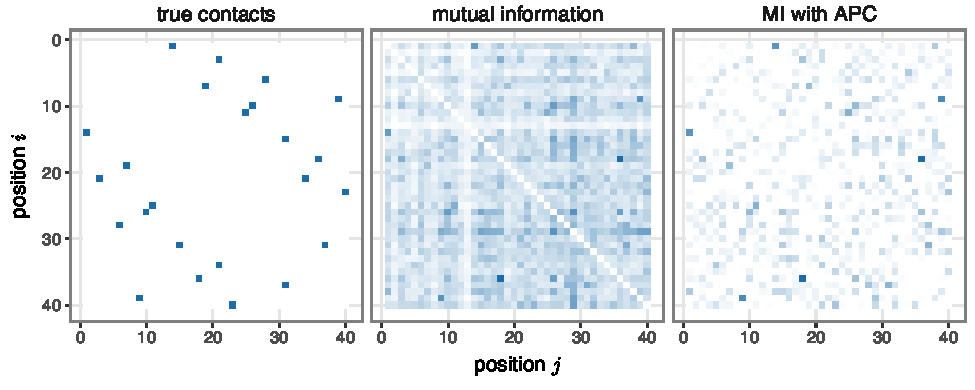
\includegraphics[width=\linewidth]{coevolution.pdf}
  \caption{Contact prediction from coevolution on a simulated alignment of 256 sequences and 40 positions, evolved down a binary tree under a Potts model~\eqref{eq:potts} with 12 planted contacts. Left: true contacts. Middle: mutual information between columns, scaled to a maximum of one. Right: mutual information after the average product correction, negative values set to zero. Phylogenetic structure gives every pair of variable columns some mutual information; the correction removes much of it.}
  \label{fig:coevolution}
\end{figure}

\subsection{From contacts to structure}

Coevolution-based contact maps, fed to physics-based folding programs, gave the first accurate predictions of the structures of large protein families from sequence alone~\citep{marks2011}. Deep learning then replaced the statistical models: convolutional networks applied to the pair features of an MSA predicted contacts, and then full \emph{distograms}, probability distributions over the distance between every pair of residues. AlphaFold~1~\citep{senior2020} predicted distograms with a deep residual network and then found a structure by gradient descent on a potential built from them.

A distance map is a strong constraint on structure but not the same thing as a structure. Given exact pairwise distances, the structure is determined only up to rotation, translation and mirror reflection; given noisy or partial distances, there may be no structure that satisfies all of them. AlphaFold~2 differs from its predecessors in predicting the coordinates directly, with a model trained end to end from sequence and MSA to structure~\citep{jumper2021}, an approach also pursued by \citet{alquraishi2019}. Its authors identify this end-to-end training as one of the reasons for its accuracy.

%======================================================================
\section{Overview of AlphaFold~2}
\label{sec:overview}
%======================================================================

Figure~\ref{fig:af2_arch} shows the architecture. Starting from the input sequence, there are three steps.

\begin{enumerate}
  \item \emph{Inputs.} A genetic database search builds an MSA of homologs, and a structure database search finds \emph{templates}, homologs whose structures are in the PDB. Templates are optional; the model works without them. The MSA is embedded as the \emph{MSA representation}, a tensor of shape $S\times R\times D_m$, with one $D_m$-dimensional vector $\vm_{si}$ for each sequence $s$ and residue $i$. Pair features are embedded as the \emph{pair representation}, of shape $R\times R\times D_z$, with one vector $\vz_{ij}$ for each pair of residues. The pair representation is initialized from the target sequence alone (the ``pairing'' step in Figure~\ref{fig:af2_arch}): $\vz_{ij}$ is the sum of a linear embedding of the amino acid at $i$, one of the amino acid at $j$, and an embedding of the sequence separation $j-i$, which acts as a relative positional encoding (Chapter 3). Template structures, when available, add pair features such as the distances between residues in the template.
  \item \emph{Evoformer.} A stack of 48 Evoformer blocks updates the two representations, passing information between them in every block (Section~\ref{sec:evoformer}).
  \item \emph{Structure module.} The first row of the MSA representation, the one for the target sequence, is projected to the \emph{single representation} $\vs_i\in\R^{D_s}$. The structure module, eight blocks with shared weights, uses the single and pair representations to place every residue in space and outputs the coordinates of all atoms and a per-residue confidence (Section~\ref{sec:structure_module}).
\end{enumerate}
The whole network is then run again, three more times at inference, with the outputs of the previous pass added to the inputs of the next: the final pair representation, the first row of the MSA representation and the distances in the predicted structure. This \emph{recycling} lets the network refine its prediction, and acts as a further, shared-weight deepening of an already deep network. Table~\ref{tab:af2_dims} lists the sizes of the representations.

\begin{figure}[!htbp]
  \centering
  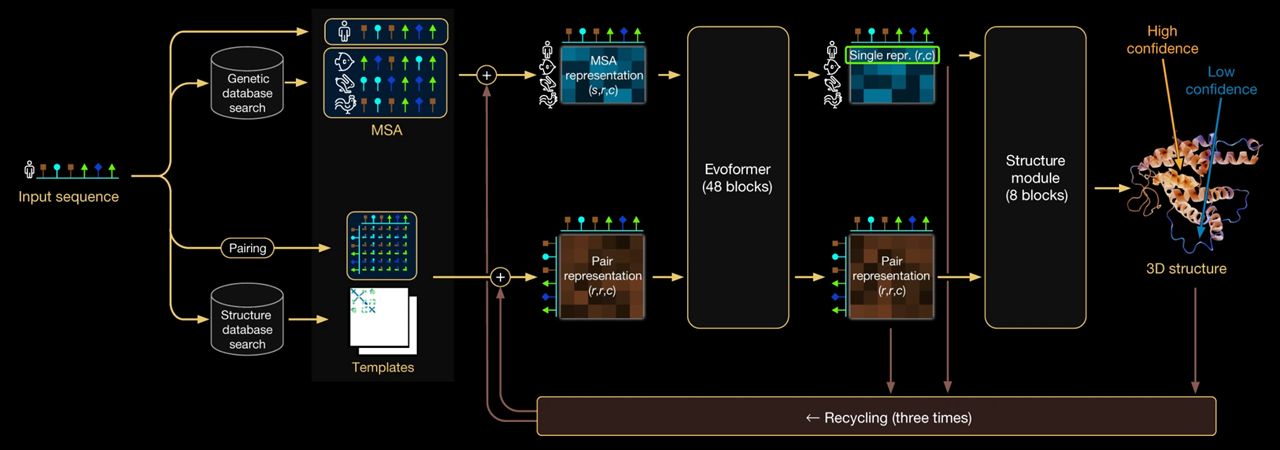
\includegraphics[width=\linewidth]{slides/alphafold2_architecture.png}
  \caption{The AlphaFold~2 architecture. The input sequence is used to search genetic and structure databases for an MSA and templates, which initialize the MSA representation ($s\times r\times c$: sequences $\times$ residues $\times$ channels) and the pair representation ($r\times r\times c$). After 48 Evoformer blocks, the single representation (the first row of the MSA representation) and the pair representation are passed to the structure module, which outputs a 3D structure coloured by predicted confidence. The whole network is recycled three times. Reproduced from \citet{jumper2021}.}
  \label{fig:af2_arch}
\end{figure}

\begin{table}[!htbp]
  \centering
  \caption{Representations in AlphaFold~2 and their sizes in the published model~\citep{jumper2021}. $R$ is the number of residues, cropped to at most 384 during training; $S$ is the number of MSA sequences processed by the main Evoformer stack (512 at inference). A further stack of four lighter blocks processes thousands of additional MSA sequences and feeds only the pair representation.}
  \label{tab:af2_dims}
  \begin{tabular}{llll}
    \toprule
    Representation & Element & Shape & Channels \\
    \midrule
    MSA & $\vm_{si}$, sequence $s$, residue $i$ & $S\times R\times D_m$ & $D_m=256$ \\
    Pair & $\vz_{ij}$, residues $i,j$ & $R\times R\times D_z$ & $D_z=128$ \\
    Single & $\vs_i$, residue $i$ & $R\times D_s$ & $D_s=384$ \\
    Backbone frames & $T_i=(\mR_i,\vt_i)$, residue $i$ & $R\times(3\times3+3)$ & -- \\
    \bottomrule
  \end{tabular}
\end{table}

The paper writes $s$, $r$ and $c$ for the numbers of sequences, residues and channels. In this chapter $S$ and $R$ are the numbers of sequences and residues, $s,t$ index sequences, $i,j,k$ index residues, and $D_m$, $D_z$, $D_s$ are channel dimensions.

%======================================================================
\section{Attention with a bias}
\label{sec:attention_recap}
%======================================================================

AlphaFold~2 contains no convolutions. Apart from position-wise linear layers and multilayer perceptrons, all of its layers are variants of attention~\citep{vaswani2017}. We use the notation of Chapter 3. For positions $i,j\in\{1,\dots,L\}$ with representations $\vh_i,\vh_j\in\R^D$, the query, key and value are $\vq_i=\mW^Q\vh_i\in\R^P$, $\vk_j=\mW^K\vh_j\in\R^P$ and $\vv_j=\mW^V\vh_j\in\R^{D_v}$, position $i$ attends to position $j$ with weight
\begin{equation}
  a_{ij} = \softmax_j\left(\frac{\vq_i^\top\vk_j}{\sqrt{P}} + b_{ij}\right) = \frac{\exp\left(\vq_i^\top\vk_j/\sqrt{P} + b_{ij}\right)}{\sum_{j'=1}^L\exp\left(\vq_i^\top\vk_{j'}/\sqrt{P} + b_{ij'}\right)},
  \label{eq:biased_attention}
\end{equation}
and its output is $\vg_i=\sum_j a_{ij}\vv_j$. Compared with Chapter 3 there is one new term, a scalar \emph{bias} $b_{ij}$ added to the score of each pair before the softmax. A positive bias makes $i$ attend more to $j$ whatever their queries and keys say, and a large negative bias forbids it. In Chapter 3 relative positional encodings could enter attention as a bias of this form, depending only on $j-i$; in AlphaFold the bias is computed from the pair representation and so carries the network's current belief about how residues $i$ and $j$ are related.

Two further details recur. AlphaFold uses multi-head attention throughout, with $M$ heads indexed by $m$, each with its own projections and bias. And most attention layers are \emph{gated}: the output of each head is multiplied elementwise by a gate $\sigm(\mW^G\vh_i)\in(0,1)^{D_v}$ computed from the input, which lets each position switch off the update from attention. Each layer is wrapped in layer normalization and a residual connection, as in the transformer block of Chapter 3. To keep the equations short we omit gating, layer normalization and bias vectors of linear layers below unless they matter for the argument; the supplementary information of \citet{jumper2021} gives them all.

%======================================================================
\section{The Evoformer}
\label{sec:evoformer}
%======================================================================

The Evoformer turns the raw MSA and pair features into representations from which a structure can be read off. Its design follows from three questions. How can attention be applied to a two-dimensional array of sequences by positions at a tolerable cost? How should information pass between the MSA and the pair representations? And how can the pair representation be encouraged to behave like a description of geometry? Figure~\ref{fig:evoformer_schematic} summarizes the answers.

\begin{figure}[!htbp]
  \centering
  \begin{tikzpicture}[>=Stealth, every node/.style={font=\small}]
    \pgfmathsetseed{14}
    % MSA representation: S x R grid
    \begin{scope}
      \fill[green!55!black!35] (-0.15,-0.15) rectangle (4.35,2.55);
      \foreach \i in {0,...,8} \foreach \s in {0,...,5} {
        \pgfmathsetmacro{\v}{20+60*rnd}
        \fill[green!\v!yellow] (0.5*\i,0.4*\s) rectangle ++(0.46,0.36);
      }
      \draw[very thick, red!80!black] (-0.05,1.57) rectangle (4.5,1.99);
      \draw[very thick, orange!90!black] (2.96,-0.08) rectangle (3.42,2.48);
      \node[above, align=center] at (2.1,2.6) {MSA representation, $S\times R\times D_m$\\ \footnotesize columns: residues $i$};
      \node[red!80!black, right] at (4.55,1.78) {row attention};
      \node[orange!90!black, below] at (3.19,-0.15) {column attention};
      \draw[decorate, decoration={brace, amplitude=4pt}] (-0.3,0) -- (-0.3,2.36) node[midway, left=5pt] {sequences $s$};
    \end{scope}
    % pair representation: R x R grid
    \begin{scope}[yshift=-6.0cm]
      \fill[blue!45] (-0.15,-0.15) rectangle (4.35,4.65);
      \foreach \i in {0,...,8} \foreach \j in {0,...,8} {
        \pgfmathsetmacro{\v}{15+60*rnd}
        \fill[green!\v!teal!70!black] (0.5*\i,0.5*\j) rectangle ++(0.46,0.46);
      }
      \node[below] at (2.1,-0.2) {pair representation, $R\times R\times D_z$};
      \draw[very thick, red!80!black] (2.46,2.96) rectangle (2.96,3.46);
      \node[white, font=\footnotesize] at (2.71,3.21) {$ij$};
      \draw[decorate, decoration={brace, mirror, amplitude=4pt}] (-0.3,4.5) -- (-0.3,0) node[midway, left=5pt] {residues $i$};
    \end{scope}
    % arrows between tracks
    \draw[->, very thick, blue!60!black] (1.0,-1.35) -- node[left, align=right, font=\footnotesize] {pair bias $b_{ij}$\\ into row attention} (1.0,-0.25);
    \draw[->, very thick, red!70!black] (3.2,-0.6) -- node[right, align=left, font=\footnotesize] {outer product mean\\ of columns $i$ and $j$} (3.2,-1.35);
    \draw[->, very thick, teal!70!black] (4.45,-3.4) arc[start angle=90, end angle=-200, radius=0.45];
    \node[right, align=left, font=\footnotesize, teal!50!black] at (5.0,-3.9) {triangle updates\\ (multiplicative and\\ attention)};
  \end{tikzpicture}
  \caption{The two tracks of the Evoformer. The MSA representation (top) is updated by axial attention, first along each row (residues of one sequence, biased by the pair representation) and then along each column (homologs at one position). The pair representation (bottom) receives the outer product mean of two columns of the MSA representation and is updated by triangle operations that couple each entry $ij$ to the entries $ik$ and $jk$. After slides by M.~AlQuraishi and N.~Bouatta.}
  \label{fig:evoformer_schematic}
\end{figure}

\subsection{Axial attention over the MSA}

The MSA representation has $S\times R$ entries. Treating each entry as a token and letting every token attend to every other would cost $(SR)^2$ attention scores per head. For $S=512$ sequences and $R=384$ residues that is about $3.9\times10^{10}$ scores, too many for each of 48 blocks. AlphaFold instead uses \emph{axial attention}~\citep{ho2019}, alternating attention along the two axes. In \emph{row-wise} attention each entry attends to the other residues of the same sequence, and in \emph{column-wise} attention to the same residue in the other sequences. The cost is $SR^2$ scores for the rows plus $RS^2$ for the columns, $SR(S+R)$ in total, about $1.8\times10^8$ for the sizes above, a saving by a factor $SR/(S+R)\approx 220$. Two rounds of axial attention connect any entry $(s,i)$ to any other $(t,j)$, through $(s,j)$.

\paragraph{Row-wise attention with pair bias.} For sequence $s$ and head $m$, the queries, keys and values are linear maps of the MSA representation, $\vq^m_{si}=\mW^{Q,m}\vm_{si}$, $\vk^m_{sj}=\mW^{K,m}\vm_{sj}$ (both in $\R^P$) and $\vv^m_{sj}=\mW^{V,m}\vm_{sj}\in\R^{D_v}$. The bias is a linear projection of the pair representation, $b^m_{ij}=\vw^{B,m\top}\LN(\vz_{ij})$ with $\vw^{B,m}\in\R^{D_z}$. Residue $i$ of sequence $s$ attends to residue $j$ of the same sequence with weight
\begin{equation}
  a^m_{sij} = \softmax_j\left(\frac{\vq^{m\top}_{si}\vk^m_{sj}}{\sqrt{P}} + b^m_{ij}\right),
  \label{eq:row_attention}
\end{equation}
and the update is
\begin{equation}
  \vm_{si} \leftarrow \vm_{si} + \mW^O\operatorname{concat}_{m=1}^{M}\Big(\sum_{j=1}^R a^m_{sij}\vv^m_{sj}\Big),
\end{equation}
with output projection $\mW^O\in\R^{D_m\times MD_v}$. The same bias $b^m_{ij}$ is used for every sequence $s$. This is how information flows from the pair representation to the MSA representation. If the pair representation encodes that residues $i$ and $j$ are close in space, the bias can make $i$ attend to $j$ in every row, so that the representation of residue $i$ in each homolog draws on that of its structural neighbours.

\paragraph{Column-wise attention.} For residue $i$, sequence $s$ attends to sequence $t$ with weight
\begin{equation}
  a^m_{sti} = \softmax_t\left(\frac{\vq^{m\top}_{si}\vk^m_{ti}}{\sqrt{P}}\right),
\end{equation}
and $\vm_{si}\leftarrow\vm_{si}+\mW^O\operatorname{concat}_m\big(\sum_{t=1}^S a^m_{sti}\vv^m_{ti}\big)$, with separate parameters from the row-wise layer. This lets each homolog's representation at position $i$ draw on the others, for example to compute the conservation of the column. A position-wise MLP (the \emph{transition}) follows, as in a transformer block. Both attention layers treat the sequences as an unordered set: permuting the rows of the MSA permutes the rows of the output and leaves the pair representation unchanged.

\subsection{From the MSA to the pair representation: the outer product mean}

Information flows from the MSA representation to the pair representation through the \emph{outer product mean}. Two linear maps reduce each entry to $D_o$ channels ($D_o=32$), $\va_{si}=\mW^A\vm_{si}$ and $\vc_{sj}=\mW^C\vm_{sj}$ in $\R^{D_o}$. For each pair of residues, the outer products of the two columns are averaged over sequences and projected to the pair channels,
\begin{equation}
  \underbrace{\vo_{ij}}_{D_o\times D_o} = \frac{1}{S}\sum_{s=1}^S \underbrace{\va_{si}}_{D_o\times1}\underbrace{\vc_{sj}^\top}_{1\times D_o}, \qquad
  \vz_{ij} \leftarrow \vz_{ij} + \mW^Z\operatorname{vec}(\vo_{ij}),
  \label{eq:opm}
\end{equation}
where $\operatorname{vec}$ stacks the $D_o^2$ entries into a vector and $\mW^Z\in\R^{D_z\times D_o^2}$. The mean removes the sequence dimension, which the pair representation does not have, and is the simplest way to do so for any number of sequences and in a way that does not depend on their order.

The outer product mean computes coevolution statistics. Substituting the linear maps,
\begin{equation}
  \vo_{ij} = \mW^A\Big(\frac{1}{S}\sum_{s=1}^S\vm_{si}\vm_{sj}^\top\Big)\mW^{C\top},
\end{equation}
a linear function of the matrix of second moments between columns $i$ and $j$ of the MSA representation. If the MSA representation were the raw one-hot encoding, $\vm_{si}=\ve_{x_{si}}\in\{0,1\}^q$, the matrix in brackets would be exactly the pair frequency table $\mF_{ij}\in\R^{q\times q}$ with entries $f_{ij}(a,b)$ from~\eqref{eq:msa_freqs}, the quantity from which mutual information and coupling estimates are computed. In AlphaFold the $\vm_{si}$ are learned features that have already passed through row and column attention, and the outer product mean is applied in every block, so the network can learn richer and more refined pair statistics than those of Section~\ref{sec:evolution}.

\subsection{The triangle inequality and triangle updates}

The pair representation is meant to encode the geometry of the protein, roughly how close each pair of residues is. Geometric quantities satisfy constraints that arbitrary arrays do not. Let $\vx_i\in\R^3$ be the position of residue $i$ (say of its \Ca) and $d_{ij}=\|\vx_i-\vx_j\|$. For any three residues $i,j,k$, with $x=d_{ij}$, $y=d_{ik}$ and $z=d_{jk}$ the lengths of the sides of the triangle they form, the \emph{triangle inequality} requires
\begin{equation}
  z \leq x + y ,
\end{equation}
and likewise for the other two sides (Figure~\ref{fig:triangle}a). If the entries of the pair representation were updated independently of one another, for instance by a position-wise MLP, nothing would make them consistent in this sense. Figure~\ref{fig:triangle}c shows how easily independent errors break consistency: adding independent noise with a standard deviation of 1\,\AA{} to the true \Ca{} distances of a helix makes about a quarter of all triples of residues violate the triangle inequality, so that no set of coordinates could produce the distances.

AlphaFold does not impose the triangle inequality as a constraint. Instead it gives the network layers in which the update of entry $ij$ depends on the entries $ik$ and $jk$ for all $k$, the other two edges of every triangle that contains edge $ij$ (Figure~\ref{fig:triangle}b), and lets it learn to use them. There are two kinds of such layers, each in two orientations.

\begin{figure}[!htbp]
  \centering
  \begin{subfigure}[b]{0.3\linewidth}
    \centering
    \begin{tikzpicture}[every node/.style={font=\small}]
      \coordinate (i) at (1.2,2.2); \coordinate (j) at (0,0); \coordinate (k) at (2.8,-0.1);
      \draw[thick] (i) -- node[above left] {$x$} (j) -- node[below] {$z$} (k) -- node[above right] {$y$} cycle;
      \foreach \p/\pos in {i/above, j/left, k/right} \fill (\p) circle (0.05) node[\pos] {$\p$};
      \node at (1.4,-1.0) {$z\leq x+y$};
    \end{tikzpicture}
    \caption{}
  \end{subfigure}\hfill
  \begin{subfigure}[b]{0.3\linewidth}
    \centering
    \begin{tikzpicture}[every node/.style={font=\small}, >=Stealth]
      \fill[blue!45] (-0.1,-0.1) rectangle (3.3,3.3);
      \pgfmathsetseed{5}
      \foreach \a in {0,...,7} \foreach \b in {0,...,7} {
        \pgfmathsetmacro{\v}{15+60*rnd}
        \fill[green!\v!teal!70!black] (0.4*\a,0.4*\b) rectangle ++(0.37,0.37);
      }
      % columns/rows: i=1, j=3, k=6 ; row index r at y = 0.4*(7-r)
      \foreach \lab/\c in {i/1, j/3, k/6} {
        \node[above] at (0.4*\c+0.18,3.3) {$\lab$};
        \node[left] at (-0.1,0.4*7-0.4*\c+0.18) {$\lab$};
      }
      \draw[very thick, red!80!black] (0.4*3,0.4*6) rectangle ++(0.37,0.37);
      \node[white, font=\scriptsize] at (0.4*3+0.18,0.4*6+0.18) {$ij$};
      \draw[very thick, orange] (0.4*6,0.4*6) rectangle ++(0.37,0.37);
      \node[white, font=\scriptsize] at (0.4*6+0.18,0.4*6+0.18) {$ik$};
      \draw[very thick, orange] (0.4*6,0.4*4) rectangle ++(0.37,0.37);
      \node[white, font=\scriptsize] at (0.4*6+0.18,0.4*4+0.18) {$jk$};
      \draw[->, thick, orange] (0.4*6,0.4*6+0.18) -- (0.4*3+0.4,0.4*6+0.18);
      \draw[->, thick, orange] (0.4*6,0.4*4+0.3) -- (0.4*3+0.4,0.4*6+0.05);
    \end{tikzpicture}
    \caption{}
  \end{subfigure}\hfill
  \begin{subfigure}[b]{0.36\linewidth}
    \centering
    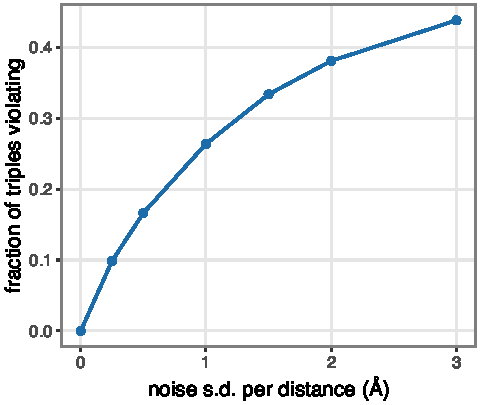
\includegraphics[width=\linewidth]{triangle_violations.pdf}
    \caption{}
  \end{subfigure}
  \caption{(a) Three residues $i,j,k$ and the distances between them, which satisfy the triangle inequality. (b) In a triangle update, the entry $ij$ of the pair representation is updated from the entries $ik$ and $jk$, for every third residue $k$ (here for one $k$, and for the ``outgoing'' orientation). (c) Fraction of the triples of residues of an ideal 30-residue $\alpha$-helix whose distances violate the triangle inequality when each pairwise \Ca{} distance is perturbed by independent Gaussian noise (20 replicates per noise level). A long helix has many nearly collinear triples (in half of all triples the longest side is within 1\,\AA{} of the sum of the other two), so small independent errors already make the distances inconsistent. (a,b) after slides by M.~AlQuraishi and N.~Bouatta.}
  \label{fig:triangle}
\end{figure}

\paragraph{Triangle multiplicative updates.} Two gated linear maps of the pair representation give $\va_{ij}=\sigm(\mW^{A_1}\vz_{ij})\odot\mW^{A_2}\vz_{ij}$ and $\vc_{ij}=\sigm(\mW^{C_1}\vz_{ij})\odot\mW^{C_2}\vz_{ij}$, both in $\R^{D_t}$ (new maps, unrelated to those of the outer product mean), where $\odot$ is the elementwise product. The update ``using outgoing edges'' is
\begin{equation}
  \vz_{ij} \leftarrow \vz_{ij} + \vg_{ij}\odot\mW^O\LN\Big(\sum_{k=1}^R \va_{ik}\odot\vc_{jk}\Big), \qquad \vg_{ij} = \sigm(\mW^G\vz_{ij}),
  \label{eq:tri_mult}
\end{equation}
which combines the two edges leaving $i$ and $j$ towards each third residue $k$. The update ``using incoming edges'' replaces the sum by $\sum_k\va_{ki}\odot\vc_{kj}$. Both orientations are needed because the pair representation is not symmetric: $\vz_{ij}$ and $\vz_{ji}$ are different vectors. For each channel $d$, the sum $\sum_k a_{ik,d}\,c_{jk,d}$ is entry $ij$ of the matrix product $\mathbf{A}_d\mathbf{C}_d^\top$ of the $R\times R$ matrices of channel $d$, so the layer costs $O(R^3D_t)$. An intuition: if $\mathbf{A}_d$ and $\mathbf{C}_d$ were both the contact map, $\sum_k a_{ik}c_{jk}$ would count the residues in contact with both $i$ and $j$. Two residues with many common neighbours are likely to be close themselves, which is the kind of reasoning the triangle inequality supports.

\paragraph{Triangle self-attention.} Fix residue $i$ and view row $i$ of the pair representation, the edges $(i,1),\dots,(i,R)$, as a sequence. In triangle attention ``around the starting node'' edge $ij$ attends to edge $ik$, with a bias from the third edge $jk$,
\begin{equation}
  a^m_{ijk} = \softmax_k\left(\frac{\vq^{m\top}_{ij}\vk^m_{ik}}{\sqrt{P}} + b^m_{jk}\right), \qquad
  \vz_{ij} \leftarrow \vz_{ij} + \mW^O\operatorname{concat}_m\Big(\sum_{k=1}^R a^m_{ijk}\vv^m_{ik}\Big),
  \label{eq:tri_att}
\end{equation}
where queries, keys and values are linear maps of the pair representation, $\vq^m_{ij}=\mW^{Q,m}\vz_{ij}$ and so on, and $b^m_{jk}=\vw^{B,m\top}\vz_{jk}$. Triangle attention ``around the ending node'' does the same along columns: edge $ij$ attends to edge $kj$ with bias from $ki$. Each costs $O(R^3)$ scores per head, more than any other layer for long proteins. Triangle attention is the pair-representation analogue of row-wise attention with pair bias: in both, which other elements to attend to is informed by the pair representation.

\subsection{The Evoformer block}

Algorithm~\ref{alg:evoformer} lists the operations of one Evoformer block. Each is wrapped in a residual connection, so the block computes a sequence of additive updates to the two representations. The block is repeated 48 times with separate parameters, so information passes between the two tracks 48 times. The representations that come out are abstract: their channels have no predefined meaning, and although the pair representation is intended to encode geometry and to be approximately consistent with the triangle inequality, nothing in the architecture forces it to be. The geometry becomes explicit only in the structure module.

\begin{algorithm}[!htbp]
  \caption{One Evoformer block. Inputs are the MSA representation $\{\vm_{si}\}$ ($S\times R\times D_m$) and the pair representation $\{\vz_{ij}\}$ ($R\times R\times D_z$).}
  \label{alg:evoformer}
  \begin{algorithmic}[1]
    \State $\vm \gets \vm + \text{RowAttentionWithPairBias}(\vm,\vz)$ \Comment{\eqref{eq:row_attention}; pair $\to$ MSA}
    \State $\vm \gets \vm + \text{ColumnAttention}(\vm)$
    \State $\vm \gets \vm + \text{Transition}(\vm)$ \Comment{position-wise MLP}
    \State $\vz \gets \vz + \text{OuterProductMean}(\vm)$ \Comment{\eqref{eq:opm}; MSA $\to$ pair}
    \State $\vz \gets \vz + \text{TriangleMultiplicationOutgoing}(\vz)$ \Comment{\eqref{eq:tri_mult}}
    \State $\vz \gets \vz + \text{TriangleMultiplicationIncoming}(\vz)$
    \State $\vz \gets \vz + \text{TriangleAttentionStartingNode}(\vz)$ \Comment{\eqref{eq:tri_att}}
    \State $\vz \gets \vz + \text{TriangleAttentionEndingNode}(\vz)$
    \State $\vz \gets \vz + \text{Transition}(\vz)$
    \State \Return $\vm,\vz$
  \end{algorithmic}
\end{algorithm}

%======================================================================
\section{The structure module}
\label{sec:structure_module}
%======================================================================

The structure module receives the single representation $\vs_i\in\R^{D_s}$, for $i=1,\dots,R$, and the pair representation $\vz_{ij}$ from the last Evoformer block, and outputs the coordinates of every atom. It does so by placing each residue in space as a rigid body and refining the placement over eight blocks. This section describes how a residue's placement is represented, why the module must respect rotations and translations, and the attention layer that makes it do so.

\subsection{Backbone frames}

Fixing bond lengths and angles at their ideal values, the backbone atoms N, \Ca{} and C of a residue form a rigid triangle (Figure~\ref{fig:backbone}). Placing this triangle in space takes six numbers: three for its position and three for its orientation. AlphaFold represents the placement of residue $i$ as a \emph{frame}, or rigid transformation,
\begin{equation}
  T_i = (\mR_i,\vt_i), \qquad \mR_i\in\SO, \quad \vt_i\in\R^3,
\end{equation}
where $\vt_i$ is the position of the \Ca{} atom and $\mR_i$ is a rotation matrix, an element of the group $\SO=\{\mR\in\R^{3\times3}:\mR^\top\mR=\mI,\ \det\mR=1\}$ of rotations of three-dimensional space (Figure~\ref{fig:frame}). The columns of $\mR_i$ are the axes of a local coordinate system attached to the residue, written in global coordinates. A point with local coordinates $\vx\in\R^3$ has global coordinates
\begin{equation}
  T_i\circ\vx = \mR_i\vx + \vt_i ,
  \label{eq:frame_action}
\end{equation}
rotate first, then translate. The inverse maps global coordinates to local ones, subtracting the translation first and then undoing the rotation,
\begin{equation}
  T_i^{-1}\circ\vx = \mR_i^\top(\vx - \vt_i), \qquad T_i^{-1} = (\mR_i^\top,\,-\mR_i^\top\vt_i),
\end{equation}
using $\mR_i^{-1}=\mR_i^\top$. Composing two frames gives a frame, $T_a\circ T_b = (\mR_a\mR_b,\ \mR_a\vt_b+\vt_a)$, as can be checked by applying both sides to a point $\vx$: $T_a\circ(T_b\circ\vx)=\mR_a(\mR_b\vx+\vt_b)+\vt_a$. With these operations the set of frames is the group $\SE$ of rigid motions, the special Euclidean group. In the local frame, the backbone atoms of every residue have the same, idealized coordinates $\vx^{\text{N}}_{\text{loc}}$, $\vx^{\text{C}\alpha}_{\text{loc}}=\mathbf{0}$ and $\vx^{\text{C}}_{\text{loc}}$, so the global coordinates of the backbone of residue $i$ are $T_i\circ\vx^{\text{N}}_{\text{loc}}$, $\vt_i$ and $T_i\circ\vx^{\text{C}}_{\text{loc}}$.

Conversely, given the coordinates $\vx^{\text{N}}_i,\vx^{\text{C}\alpha}_i,\vx^{\text{C}}_i$ of a residue in an experimental structure, its frame is built by Gram--Schmidt orthogonalization. With $\vu_1=\vx^{\text{C}}_i-\vx^{\text{C}\alpha}_i$ and $\vu_2=\vx^{\text{N}}_i-\vx^{\text{C}\alpha}_i$,
\begin{equation}
  \ve_1 = \frac{\vu_1}{\|\vu_1\|}, \qquad
  \ve_2 = \frac{\vu_2-(\ve_1^\top\vu_2)\ve_1}{\|\vu_2-(\ve_1^\top\vu_2)\ve_1\|}, \qquad
  \ve_3 = \ve_1\times\ve_2, \qquad
  \mR_i = [\ve_1\ \ve_2\ \ve_3], \quad \vt_i = \vx^{\text{C}\alpha}_i .
  \label{eq:gram_schmidt}
\end{equation}
The vectors $\ve_1$ and $\ve_2$ are orthonormal and span the plane of the three atoms, and the cross product $\ve_3$ completes them to a right-handed basis, so $\det\mR_i=1$.

\begin{figure}[!htbp]
  \centering
  \begin{tikzpicture}[>=Stealth, every node/.style={font=\small}]
    % global axes
    \draw[->, thick] (0,0) -- (2.4,0) node[right] {$x$};
    \draw[->, thick] (0,0) -- (0,2.2) node[above] {$y$};
    \draw[->, thick] (0,0) -- (-1.1,-1.0) node[below left] {$z$};
    \node[below right] at (0,0) {global origin};
    % residue triangle
    \coordinate (CA) at (5.5,2.0); \coordinate (Cc) at (6.9,1.6); \coordinate (Nn) at (5.0,0.9);
    \fill[red!15, draw=red!70!black, thick] (Nn) -- (CA) -- (Cc) -- cycle;
    \foreach \p/\l/\pos in {CA/C$\alpha$/above, Cc/C/right, Nn/N/below left} \fill (\p) circle (0.06) node[\pos] {\l};
    % translation
    \draw[->, very thick, blue!70!black] (0,0) -- node[below right, pos=0.55] {$\vt_i$} (CA);
    % local axes
    \draw[->, thick, orange!90!black] (CA) -- ($(CA)!1.1cm!(Cc)$) node[above right] {$\ve_1$};
    \draw[->, thick, orange!90!black] (CA) -- ++(-0.45,-0.85) node[left] {$\ve_2$};
    \draw[->, thick, orange!90!black] (CA) -- ++(0.15,1.05) node[above] {$\ve_3$};
    \node[orange!70!black, align=left] at (9.2,2.3) {$\mR_i=[\ve_1\ \ve_2\ \ve_3]$\\ local axes in\\ global coordinates};
    \node at (8.6,0.5) {$T_i=(\mR_i,\vt_i)$};
  \end{tikzpicture}
  \caption{The frame of residue $i$. The translation $\vt_i$ is the position of the \Ca{} atom, and the columns of the rotation $\mR_i$ are the axes of a local coordinate system attached to the N--\Ca--C triangle, built from the atom positions by~\eqref{eq:gram_schmidt}. The axis $\ve_3$ points out of the plane of the triangle. After a slide by M.~AlQuraishi and N.~Bouatta.}
  \label{fig:frame}
\end{figure}

\subsection{The residue gas}

In a real protein the triangles are chained together: the C atom of residue $i$ is bonded to the N atom of residue $i+1$ at a distance of about 1.33\,\AA. Constraints like this are awkward for a neural network to impose exactly. AlphaFold does not impose them. It treats the protein as a \emph{residue gas}, a bag of $R$ independent triangles, each free to move and rotate, with $6R$ degrees of freedom in total. The network must learn that consecutive residues belong next to each other; at the end of training a loss term penalizes violated bond lengths and angles and clashes between atoms. Ignoring the chain makes every residue's update local and parallel, so that all parts of the structure can be refined at the same time rather than by propagating changes along the chain.

The structure module starts from what the authors call a \emph{black hole} initialization: every frame is the identity, $T_i=(\mI,\mathbf{0})$, so all residues sit at the origin with the same orientation (Figure~\ref{fig:residue_gas}a). Each of the eight blocks then moves and rotates every triangle a little, and by the last block the triangles should sit where the residues of the true structure are (Figure~\ref{fig:residue_gas}b).

\subsection{Invariance and equivariance}

A protein does not know where it is in space or which way it faces. If we rotate and translate the true structure by a global rigid motion $T_g=(\mR_g,\vt_g)$, every atom $\vx$ moves to $T_g\circ\vx$ and every frame $T_i$ to $T_g\circ T_i$, but it is the same structure. This places two requirements on the model.

A quantity computed from a structure, such as a loss or a distance, should be \emph{invariant}: $f(\{T_g\circ T_i\})=f(\{T_i\})$ for every $T_g\in\SE$. A map that updates a structure, such as one block $\varphi$ of the structure module, which takes frames $\{T_i\}$ to updated frames, should be \emph{equivariant}: it should commute with global motions,
\begin{equation}
  \varphi(\{T_g\circ T_i\}) = \{T_g\circ T'_i\}, \qquad\text{where } \{T'_i\}=\varphi(\{T_i\}).
  \label{eq:equivariance}
\end{equation}
In words, rotating the input and then updating gives the same result as updating and then rotating the output (Figure~\ref{fig:equivariance}). This is not automatic: a generic neural network applied to coordinates does not commute with rotations. It would have to learn the symmetry from data, by seeing structures in all orientations, and would still only approximate it.

The requirement is for $\SE$, rotations and translations, and not for the larger group $\mathrm{E}(3)$ that also contains reflections. A mirror image of a protein is a different molecule. Amino acids other than glycine are chiral, natural proteins are built from the L forms, and the $\alpha$-helix is right-handed; the mirror-image protein, built from D-amino acids, does not occur in nature and interacts differently with other chiral molecules. More generally in biochemistry, the two mirror-image forms of a chiral drug can have different effects. A structure predictor must therefore distinguish a structure from its mirror image.

The Evoformer raises none of these issues, because its representations contain no coordinates: the pair representation is invariant by construction, and template and recycled structures enter only through invariant features such as distances. The problem arises once frames are introduced in the structure module. AlphaFold makes each block equivariant through two components: an attention layer whose output is invariant to global motions, and an update rule that turns invariant features into equivariant frame updates.

\begin{figure}[!htbp]
  \centering
  \begin{tikzpicture}[>=Stealth, every node/.style={font=\small},
      rt/.style={draw=red!70!black, thick, fill=red!15},
      yt/.style={draw=yellow!60!black, thick, fill=yellow!30}]
    \newcommand{\ax}[1]{\draw[->, gray] #1 -- ++(1.0,0); \draw[->, gray] #1 -- ++(0,1.0); \draw[->, gray] #1 -- ++(-0.5,-0.45);}
    % (a) black hole
    \begin{scope}
      \ax{(0,0)}
      \foreach \d in {0,0.05,0.1,0.15} \draw[rt] (-0.4+\d,-0.2+\d) -- (0.1+\d,0.35+\d) -- (0.55+\d,-0.1+\d) -- cycle;
      \node at (0.3,-1.2) {(a) black hole initialization};
    \end{scope}
    % (b) residue gas
    \begin{scope}[xshift=4.8cm]
      \foreach \x/\y/\a in {-1.0/0.2/10, 0.0/0.7/-20, 0.9/0.0/35, 1.8/0.8/-5, 0.6/-0.7/60, -0.4/-0.6/-40} {
        \begin{scope}[shift={(\x,\y)}, rotate=\a]
          \draw[rt] (-0.3,-0.15) -- (0.05,0.25) -- (0.4,-0.1) -- cycle;
        \end{scope}
      }
      \node at (0.4,-1.2) {(b) residue gas};
    \end{scope}
    % (c) invariant point attention
    \begin{scope}[xshift=9.6cm]
      \foreach \x/\y/\a [count=\n] in {-1.2/-0.4/10, -0.2/-0.6/-15, 0.9/-0.5/25, 1.8/-0.3/-5} {
        \begin{scope}[shift={(\x,\y)}, rotate=\a]
          \draw[rt] (-0.3,-0.15) -- (0.05,0.25) -- (0.4,-0.1) -- cycle;
          \coordinate (k\n) at (0.05,0.6);
        \end{scope}
        \fill[red!70!black] (k\n) circle (0.06);
      }
      \begin{scope}[shift={(0.3,1.0)}, rotate=-10]
        \draw[yt] (-0.3,-0.15) -- (0.05,0.25) -- (0.4,-0.1) -- cycle;
        \coordinate (q) at (0.1,-0.45);
      \end{scope}
      \fill[yellow!50!black] (q) circle (0.06);
      \foreach \n in {1,...,4} \draw[gray] (q) -- (k\n);
      \node[yellow!40!black, font=\footnotesize] at (1.3,1.25) {residue $i$};
      \node at (0.3,-1.2) {(c) invariant point attention};
    \end{scope}
  \end{tikzpicture}
  \caption{(a) The structure module starts with every residue's triangle at the origin with the identity orientation. (b) Its blocks move each triangle independently; the residues are not explicitly chained (the residue gas). (c) In invariant point attention, residue $i$ (yellow) attends to residue $j$ (red) more when the query point it places in its own frame is close, in global space, to the key point that residue $j$ places in its frame. After slides by M.~AlQuraishi and N.~Bouatta.}
  \label{fig:residue_gas}
\end{figure}

\begin{figure}[!htbp]
  \centering
  \begin{tikzpicture}[>=Stealth, every node/.style={font=\small},
      rt/.style={draw=red!70!black, thick, fill=red!15},
      yt/.style={draw=yellow!60!black, thick, fill=yellow!30}]
    \newcommand{\gas}[2]{%
      \begin{scope}[shift={#1}, rotate=#2]
        \draw[->, gray] (0,0) -- (0.9,0); \draw[->, gray] (0,0) -- (0,0.9);
        \foreach \x/\y/\a in {0.1/0.15/0, 0.45/0.5/30, 0.75/0.1/-20} {
          \begin{scope}[shift={(\x,\y)}, rotate=\a] \draw[rt] (-0.15,-0.08) -- (0.02,0.12) -- (0.2,-0.05) -- cycle; \end{scope}
        }
      \end{scope}}
    \newcommand{\gasb}[2]{%
      \begin{scope}[shift={#1}, rotate=#2]
        \draw[->, gray] (0,0) -- (0.9,0); \draw[->, gray] (0,0) -- (0,0.9);
        \foreach \x/\y/\a in {0.25/0.25/40, 0.6/0.7/-10, 0.95/0.35/70} {
          \begin{scope}[shift={(\x,\y)}, rotate=\a] \draw[yt] (-0.15,-0.08) -- (0.02,0.12) -- (0.2,-0.05) -- cycle; \end{scope}
        }
      \end{scope}}
    \gas{(0,2.6)}{0}
    \gas{(5.2,2.4)}{35}
    \gasb{(0,0)}{0}
    \gasb{(5.2,-0.2)}{35}
    \node at (0.5,3.9) {$\{T_i\}$};
    \node at (5.3,3.9) {$\{T_g\circ T_i\}$};
    \node at (0.5,-0.55) {$\{T'_i\}$};
    \node at (5.3,-0.55) {$\{T_g\circ T'_i\}$};
    \draw[->, thick, teal!70!black] (1.6,3.0) -- node[above] {$T_g\in\SE$} (4.3,3.0);
    \draw[->, thick, teal!70!black] (1.6,0.4) -- node[below] {$T_g$} (4.4,0.4);
    \draw[->, thick, teal!70!black] (0.5,2.4) -- node[left] {$\varphi$} (0.5,1.3);
    \draw[->, thick, teal!70!black] (5.0,2.2) -- node[right] {$\varphi$} (5.0,1.3);
  \end{tikzpicture}
  \caption{Equivariance of a structure module block $\varphi$. Applying a global rotation and translation $T_g$ and then the block (right path) gives the same frames as applying the block and then $T_g$ (left and bottom path). After a slide by M.~AlQuraishi and N.~Bouatta.}
  \label{fig:equivariance}
\end{figure}

\subsection{Invariant point attention}

\emph{Invariant point attention} (IPA) updates the single representation using the single and pair representations and the current frames. It is attention over residues with three terms in the score. For head $m$, the first two are as in~\eqref{eq:row_attention}: an inner product of a query $\vq^m_i$ and key $\vk^m_j$ computed from $\vs_i$ and $\vs_j$, and a bias $b^m_{ij}$ projected from $\vz_{ij}$. Neither involves coordinates. The third is geometric. Each residue also produces $N_q$ query points $\vq^{mp}_i\in\R^3$ and key points $\vk^{mp}_j\in\R^3$, $p=1,\dots,N_q$, by linear maps of $\vs_i$, and these are interpreted as points in the residue's \emph{local} frame. Residue $i$ attends to residue $j$ more when its query points, placed in space by its frame, land close to the key points of residue $j$ placed by $j$'s frame,
\begin{equation}
  a^m_{ij} = \softmax_j\left( w_L\left( \frac{\vq^{m\top}_i\vk^m_j}{\sqrt{P}} + b^m_{ij} - \frac{\gamma^m w_C}{2}\sum_{p=1}^{N_q}\big\|T_i\circ\vq^{mp}_i - T_j\circ\vk^{mp}_j\big\|^2 \right)\right),
  \label{eq:ipa}
\end{equation}
where $\gamma^m>0$ is a learned weight per head and $w_L$, $w_C$ are fixed constants that keep the three terms on comparable scales. The squared distance enters with a minus sign, so nearby points increase the attention weight. In the published model there are $M=12$ heads and $N_q=4$ query points per head.

The output for residue $i$ combines three kinds of values with the same attention weights: scalar values $\vv^m_j$ computed from $\vs_j$, the pair representation $\vz_{ij}$, and $N_v$ value points $\vv^{mp}_j\in\R^3$ in the local frame of $j$. The value points are moved to global coordinates, averaged, and moved back into the local frame of $i$,
\begin{equation}
  \vo^{m}_i=\sum_j a^m_{ij}\vv^m_j, \qquad
  \tilde\vo^{m}_i=\sum_j a^m_{ij}\vz_{ij}, \qquad
  \vo^{mp}_i = T_i^{-1}\circ\Big(\sum_{j=1}^R a^m_{ij}\, T_j\circ\vv^{mp}_j\Big),
  \label{eq:ipa_out}
\end{equation}
and $\vs_i$ is updated by a linear map of the concatenation of all these outputs and the norms $\|\vo^{mp}_i\|$.

\paragraph{Why the output is invariant.} Apply a global motion to all frames, $T_j\mapsto T_g\circ T_j$ for every $j$, while $\vs$ and $\vz$, which carry no coordinates, are unchanged. The local points $\vq^{mp}_i$, $\vk^{mp}_j$ and $\vv^{mp}_j$ are computed from $\vs$ and so are unchanged too. In the score,
\begin{equation}
  (T_g\circ T_i)\circ\vq - (T_g\circ T_j)\circ\vk = \big(\mR_g(T_i\circ\vq)+\vt_g\big) - \big(\mR_g(T_j\circ\vk)+\vt_g\big) = \mR_g\big(T_i\circ\vq - T_j\circ\vk\big),
\end{equation}
the translation cancels, and the rotation does not change the norm, $\|\mR_g\vu\|^2=\vu^\top\mR_g^\top\mR_g\vu=\|\vu\|^2$. So every $a^m_{ij}$ is unchanged. For the point output, using $\sum_j a^m_{ij}=1$,
\begin{align}
  (T_g\circ T_i)^{-1}\circ\Big(\sum_j a^m_{ij}\,(T_g\circ T_j)\circ\vv^{mp}_j\Big)
  &= T_i^{-1}\circ T_g^{-1}\circ\Big(\mR_g\sum_j a^m_{ij}\,T_j\circ\vv^{mp}_j + \vt_g\Big) \nonumber\\
  &= T_i^{-1}\circ\Big(\sum_j a^m_{ij}\,T_j\circ\vv^{mp}_j\Big) = \vo^{mp}_i ,
\end{align}
since $T_g^{-1}\circ(\mR_g\vu+\vt_g)=\vu$. The weights summing to one is what lets the translation pass through the average. All outputs, and therefore the updated $\vs_i$, are invariant. The geometric term gives the network a way to reason about which residues are near which in the current structure, while its output stays independent of the global frame.

\subsection{Updating the frames}

After IPA and a transition MLP, a linear layer predicts from each $\vs_i$ an update to frame $i$: a vector $\boldsymbol{\kappa}_i\in\R^3$ that defines a rotation through the unit quaternion $(1,\kappa_{i1},\kappa_{i2},\kappa_{i3})/\sqrt{1+\|\boldsymbol{\kappa}_i\|^2}$, and a translation $\vt^{\text{upd}}_i\in\R^3$. For a unit quaternion $(\eta_0,\eta_1,\eta_2,\eta_3)$ the rotation matrix is
\begin{equation}
  \mR = \begin{pmatrix}
    \eta_0^2+\eta_1^2-\eta_2^2-\eta_3^2 & 2(\eta_1\eta_2-\eta_0\eta_3) & 2(\eta_1\eta_3+\eta_0\eta_2)\\
    2(\eta_1\eta_2+\eta_0\eta_3) & \eta_0^2-\eta_1^2+\eta_2^2-\eta_3^2 & 2(\eta_2\eta_3-\eta_0\eta_1)\\
    2(\eta_1\eta_3-\eta_0\eta_2) & 2(\eta_2\eta_3+\eta_0\eta_1) & \eta_0^2-\eta_1^2-\eta_2^2+\eta_3^2
  \end{pmatrix},
\end{equation}
which is a valid rotation for any $\boldsymbol{\kappa}_i$, and close to the identity when $\boldsymbol{\kappa}_i$ is small. Fixing the first component to one keeps each update a modest rotation. The update is composed on the right,
\begin{equation}
  T_i \leftarrow T_i\circ T^{\text{upd}}_i, \qquad T^{\text{upd}}_i=(\mR^{\text{upd}}_i,\vt^{\text{upd}}_i),
  \label{eq:frame_update}
\end{equation}
so that it is expressed in the residue's local frame: $\vt^{\text{upd}}_i$ is a step along the residue's own axes.

\paragraph{Why the update is equivariant.} Because $\vs_i$ is invariant, so is $T^{\text{upd}}_i$. If all frames are first moved to $T_g\circ T_i$, the updated frame is $(T_g\circ T_i)\circ T^{\text{upd}}_i = T_g\circ(T_i\circ T^{\text{upd}}_i)$ by associativity, which is the global motion applied to the frame updated without it. This is exactly the equivariance~\eqref{eq:equivariance}. Composing on the left, $T^{\text{upd}}_i\circ T_i$, would not work, because an update predicted from invariant features would then move every residue along the same global axes whatever the orientation of the protein.

\subsection{Side chains}

The frames place the backbone. For the side chains, a small residual network predicts seven torsion angles per residue from $\vs_i$: the backbone torsions $\omega$, $\phi$, $\psi$ and the side-chain torsions $\chi_1,\dots,\chi_4$ (unused ones are ignored). An angle lives on a circle, not on the real line: $359^\circ$ and $1^\circ$ are close. Each angle is therefore predicted as an unnormalized vector in $\R^2$ and normalized onto the unit circle, giving $(\cos\theta,\sin\theta)$ without a discontinuity. A pair of angles such as $(\phi,\psi)$ lives on a torus, the product of two circles, on which the Ramachandran plot is naturally drawn. Given the frames and torsion angles, the coordinates of all side-chain atoms follow from idealized bond geometry: each side chain is a chain of rigid groups, each rotated about a bond by one torsion angle relative to the previous group. Since the torsions are computed from the invariant $\vs_i$ and the atoms are placed relative to the frame $T_i$, the full-atom structure is equivariant too.

\subsection{Iterative refinement and recycling}

Algorithm~\ref{alg:structure_module} summarizes the structure module. The eight blocks share their weights, so the module applies the same update repeatedly, moving the residues step by step from the black hole towards the structure, much as an iterative algorithm would. Unlike the hidden layers of a typical network, the state after each block is already a structure, which is what makes the intermediate losses of the next section possible. Recycling wraps the whole network in a second loop (Algorithm~\ref{alg:recycling}), so that inference is a nested loop of refinement.

\begin{algorithm}[!htbp]
  \caption{Structure module (simplified). $\vs_i\in\R^{D_s}$ and $\vz_{ij}\in\R^{D_z}$ come from the Evoformer.}
  \label{alg:structure_module}
  \begin{algorithmic}[1]
    \State $T_i\gets(\mI,\mathbf{0})$ for all $i$ \Comment{black hole initialization}
    \For{$\ell=1,\dots,8$} \Comment{shared weights}
      \State $\vs \gets \vs + \text{IPA}(\vs,\vz,\{T_i\})$ \Comment{\eqref{eq:ipa}--\eqref{eq:ipa_out}; invariant}
      \State $\vs \gets \vs + \text{Transition}(\vs)$
      \State $T_i \gets T_i\circ\text{BackboneUpdate}(\vs_i)$ for all $i$ \Comment{\eqref{eq:frame_update}; equivariant}
      \State predict torsion angles from $\vs_i$; compute backbone loss terms for this block
    \EndFor
    \State compute all atom coordinates from $\{T_i\}$ and the torsion angles
  \end{algorithmic}
\end{algorithm}

\begin{algorithm}[!htbp]
  \caption{AlphaFold~2 inference with recycling.}
  \label{alg:recycling}
  \begin{algorithmic}[1]
    \State search databases for the MSA and templates of the input sequence
    \State set the recycled features to zero
    \For{$c=0,1,2,3$} \Comment{three recycling iterations after the first pass}
      \State embed MSA, templates and pair features; add the recycled features
      \State $(\vm,\vz)\gets$ 48 Evoformer blocks (Algorithm~\ref{alg:evoformer}); $\vs_i\gets$ linear map of $\vm_{1i}$
      \State structure, confidence $\gets$ structure module (Algorithm~\ref{alg:structure_module})
      \State recycled features $\gets$ first MSA row $\vm_{1\cdot}$, pair representation $\vz$, distances in the predicted structure
    \EndFor
  \end{algorithmic}
\end{algorithm}

%======================================================================
\section{Training}
\label{sec:training}
%======================================================================

AlphaFold~2 is trained end to end, from MSA and templates to atom coordinates, on structures from the PDB. The loss has several terms. The main one compares predicted and true structures; the others supervise intermediate outputs and auxiliary predictions.

\subsection{Frame aligned point error}

Comparing two structures requires care, because the prediction lives in an arbitrary global frame. The usual metric, the root mean square deviation (RMSD) of atom positions, first superimposes the prediction on the truth by the rotation and translation that minimize it. A single global superposition is dominated by the largest errors: if two domains are each predicted well but their relative orientation is wrong, no superposition fits both. An alternative that needs no superposition is the distance RMSD (dRMSD), which compares all pairwise distances, $\sqrt{\text{mean}_{i<j}(d_{ij}-d^{\text{true}}_{ij})^2}$. Distances are invariant to rotations and translations, but also to reflections, so a mirror image of the true structure has a dRMSD of zero.

The \emph{frame aligned point error} (FAPE) avoids both problems by aligning on every residue in turn. For each frame $i$ and each atom $j$, it expresses the atom in the residue's local frame, in both the predicted and the true structure,
\begin{equation}
  \vx_{ij} = T_i^{-1}\circ\vx_j, \qquad \vx^{\text{true}}_{ij} = (T_i^{\text{true}})^{-1}\circ\vx^{\text{true}}_j ,
\end{equation}
where $\vx_j\in\R^3$ is the predicted global position of atom $j$, and the true frames $T^{\text{true}}_i$ are built from the experimental coordinates by~\eqref{eq:gram_schmidt}. The error for the pair is
\begin{equation}
  d_{ij} = \sqrt{\big\|\vx_{ij} - \vx^{\text{true}}_{ij}\big\|^2 + \varepsilon},
\end{equation}
and the loss averages a clamped version over all $N_{\text{frames}}$ frames and $N_{\text{atoms}}$ atoms,
\begin{equation}
  \mathcal{L}_{\text{FAPE}} = \frac{1}{Z}\,\frac{1}{N_{\text{frames}}N_{\text{atoms}}}\sum_{i=1}^{N_{\text{frames}}}\sum_{j=1}^{N_{\text{atoms}}}\min\left(d_{\text{clamp}},\,d_{ij}\right),
  \label{eq:fape}
\end{equation}
with $d_{\text{clamp}}=10$\,\AA, $Z=10$\,\AA{} a length scale that makes the loss unitless, and $\varepsilon=10^{-4}$\,\AA$^2$ (Figure~\ref{fig:fape}a). The small $\varepsilon$ inside the square root makes $d_{ij}$ differentiable everywhere: the Euclidean norm $\|\vu\|$ has gradient $\vu/\|\vu\|$, which has unit length however small $\vu$ is and is undefined at $\vu=\mathbf{0}$, while $\sqrt{\|\vu\|^2+\varepsilon}$ is smooth and equals $\|\vu\|$ to within a small fraction of an \aa{}ngstr\"om. Clamping stops gross errors, such as a misplaced domain, from dominating the gradient, so that the loss rewards getting local structure right; in most training examples the clamp is applied.

\paragraph{Invariance.} Apply a global motion $T_g$ to the predicted structure, so that $T_i\mapsto T_g\circ T_i$ and $\vx_j\mapsto T_g\circ\vx_j$. Then
\begin{equation}
  (T_g\circ T_i)^{-1}\circ(T_g\circ\vx_j) = T_i^{-1}\circ T_g^{-1}\circ T_g\circ\vx_j = T_i^{-1}\circ\vx_j = \vx_{ij},
\end{equation}
so FAPE is unchanged, and the same holds for the true structure. No superposition step is needed: each frame defines its own alignment, and FAPE averages the error over $N_{\text{frames}}$ different alignments.

\paragraph{Reflections.} FAPE does distinguish a structure from its mirror image. Let $\mM$ be a reflection, an orthogonal matrix with $\det\mM=-1$, for example $\operatorname{diag}(1,1,-1)$, and suppose the predicted atoms are the reflected true atoms, $\vx_j=\mM\vx^{\text{true}}_j$. In the Gram--Schmidt construction~\eqref{eq:gram_schmidt}, $\vu_1$ and $\vu_2$ become $\mM\vu_1$ and $\mM\vu_2$, so $\ve_1\mapsto\mM\ve_1$ and $\ve_2\mapsto\mM\ve_2$. For an orthogonal $\mM$, $(\mM\va)\times(\mM\vc)=\det(\mM)\,\mM(\va\times\vc)$, so $\ve_3\mapsto-\mM\ve_3$. The predicted frame is therefore $\mR_i=\mM\mR^{\text{true}}_i\mathbf{D}$ with $\mathbf{D}=\operatorname{diag}(1,1,-1)$ and $\vt_i=\mM\vt^{\text{true}}_i$, and the local coordinates are
\begin{equation}
  \vx_{ij} = \mathbf{D}\mR^{\text{true}\top}_i\mM^\top\mM\big(\vx^{\text{true}}_j-\vt^{\text{true}}_i\big) = \mathbf{D}\,\vx^{\text{true}}_{ij}.
\end{equation}
The third local coordinate, the height of atom $j$ above the plane of residue $i$, changes sign, so $d_{ij}\approx2|(\vx^{\text{true}}_{ij})_3|$, which is zero only for atoms in the plane of residue $i$. Figure~\ref{fig:fape}b confirms this on an ideal $\alpha$-helix. Its mirror image, a left-handed helix, has a dRMSD of zero, while its FAPE is 8.3\,\AA{} (before division by $Z$) and its superposed RMSD 3.2\,\AA. The figure also shows that FAPE responds more steeply than RMSD to errors in the backbone torsion angles: a small change of a residue's orientation moves distant atoms far in that residue's frame.

\begin{figure}[!htbp]
  \centering
  \begin{subfigure}[b]{0.44\linewidth}
    \centering
    \begin{tikzpicture}[>=Stealth, every node/.style={font=\small},
        rt/.style={draw=red!70!black, thick, fill=red!15}]
      % experimental
      \begin{scope}
        \draw[rt] (0,0) -- (0.4,0.5) -- (0.85,0.05) -- cycle;
        \draw[->, gray] (0.4,0.5) -- ++(0.7,0) ; \draw[->, gray] (0.4,0.5) -- ++(0,0.7);
        \fill[blue!60!black] (1.2,1.6) circle (0.07);
        \draw[dashed, blue!60!black] (0.4,0.5) -- (1.2,1.6);
        \node[blue!60!black, right] at (1.25,1.6) {$\vx^{\text{true}}_{ij}$};
        \node at (0.6,-0.5) {true, frame $i$};
      \end{scope}
      \begin{scope}[xshift=3.0cm]
        \draw[rt] (0,0) -- (0.4,0.5) -- (0.85,0.05) -- cycle;
        \draw[->, gray] (0.4,0.5) -- ++(0.7,0) ; \draw[->, gray] (0.4,0.5) -- ++(0,0.7);
        \fill[orange!80!black] (1.45,1.35) circle (0.07);
        \fill[blue!60!black, opacity=0.4] (1.2,1.6) circle (0.07);
        \draw[dashed, orange!80!black] (0.4,0.5) -- (1.45,1.35);
        \draw[<->, thick] (1.2,1.6) -- (1.45,1.35) node[right] {$d_{ij}$};
        \node[orange!80!black, right] at (1.5,1.0) {$\vx_{ij}$};
        \node at (0.6,-0.5) {predicted, frame $i$};
      \end{scope}
      \node[align=center, font=\footnotesize] at (2.2,-1.25) {atom $j$ in the frame of residue $i$,\\ compared after aligning frame $i$};
    \end{tikzpicture}
    \caption{}
  \end{subfigure}\hfill
  \begin{subfigure}[b]{0.54\linewidth}
    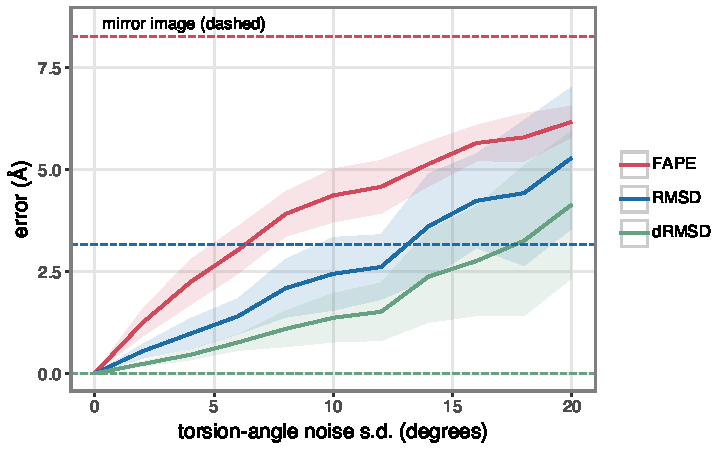
\includegraphics[width=\linewidth]{fape_vs_rmsd.pdf}
    \caption{}
  \end{subfigure}
  \caption{(a) FAPE expresses each atom $j$ in the local frame of each residue $i$, in the true and in the predicted structure, and measures the distance $d_{ij}$ between the two. (b) Errors of perturbed copies of an ideal 30-residue $\alpha$-helix, in which every $\phi$ and $\psi$ angle is perturbed by Gaussian noise and the backbone rebuilt with ideal geometry, as a function of the noise standard deviation (mean $\pm$ one s.d.\ over 30 replicates; each copy is also randomly rotated). FAPE is reported in \AA{} before division by $Z$; RMSD is the \Ca{} RMSD after optimal superposition; dRMSD compares \Ca{} distances. Dashed lines show the values for the mirror image of the helix: its dRMSD is zero.}
  \label{fig:fape}
\end{figure}

\paragraph{Which frames and atoms.} The final FAPE uses all atoms and the frames of all rigid groups, backbone and side chain. Some side chains are symmetric, for example the two oxygens of aspartate are chemically equivalent, and the true structure is relabelled to whichever naming better matches the prediction before the loss is computed.

\subsection{Auxiliary and intermediate losses}

The other terms are as follows.

\begin{itemize}
  \item \emph{Intermediate structure loss} $\mathcal{L}_{\text{aux}}$. Because the state after each block of the structure module is a structure, the loss can be computed there too. $\mathcal{L}_{\text{aux}}$ averages, over the eight blocks, a backbone-only FAPE and a loss on the predicted torsion angles. Normally a loss is computed only at the output of a network, since the hidden layers are abstract; here every block is pushed to produce a good structure, and the authors' ablations show that this helps.
  \item \emph{Distogram loss} $\mathcal{L}_{\text{dist}}$. A linear layer on the symmetrized pair representation $\vz_{ij}+\vz_{ji}$ predicts a distribution $p_{ij}(b)$ over 64 bins $b$ of the distance between the C$\beta$ atoms of residues $i$ and $j$ (\Ca{} for glycine), from 2 to 22\,\AA. The loss is the cross-entropy $-\frac{1}{R^2}\sum_{i,j}\sum_b y_{ij}(b)\log p_{ij}(b)$, where $y_{ij}(b)=1$ if the true distance falls in bin $b$ and zero otherwise. This is the AlphaFold~1 objective, kept as an auxiliary signal that supervises the pair representation directly.
  \item \emph{Masked MSA loss} $\mathcal{L}_{\text{MSA}}$. Before the MSA enters the network, 15\% of its entries are selected and corrupted: most are replaced by a mask token, and the rest by a random amino acid, by an amino acid sampled from the column's frequency profile, or left unchanged. A linear layer on the final MSA representation predicts the original residue at the selected entries, with a cross-entropy loss. This is the masked language modelling objective of BERT~\citep{devlin2019}: to fill in a masked residue the network must learn the dependencies between columns and between homologs, the coevolution signal of Section~\ref{sec:evolution}.
  \item \emph{Confidence loss} $\mathcal{L}_{\text{conf}}$, described next.
\end{itemize}

\subsection{Predicting confidence}

AlphaFold~2 predicts how accurate each part of its prediction is. The target is the \emph{local distance difference test} (lDDT)~\citep{mariani2013}, a superposition-free score. For residue $i$, take all residues $j$ whose \Ca{} atoms are within 15\,\AA{} of residue $i$'s in the true structure. For each threshold $\tau\in\{0.5,1,2,4\}$\,\AA, compute the fraction of these $j$ for which the predicted and true distances agree to within $\tau$, $|d_{ij}-d^{\text{true}}_{ij}|<\tau$. The lDDT-\Ca{} of residue $i$ is the average of the four fractions, times 100. It measures how well the local environment of each residue is reproduced, between 0 and 100.

A small network on the final single representation $\vs_i$ predicts a distribution over 50 bins of lDDT for each residue, trained by cross-entropy against the lDDT of the predicted structure computed during training. The mean of the predicted distribution is the \emph{pLDDT}, the per-residue confidence used to colour structures (Figure~\ref{fig:af2_arch}). A related head on the pair representation predicts the expected error in the position of residue $j$ when the predicted and true structures are aligned on the frame of residue $i$, which indicates whether the relative placement of two domains is reliable.

It may seem surprising that a network can predict its own errors, since neural networks are often poorly calibrated. One reason it works here is that the uncertainty has biological sources the network can learn to recognize: low pLDDT often marks intrinsically disordered regions, and shallow MSAs give less reliable predictions.

\subsection{The full objective}

The loss for the main stage of training combines the terms,
\begin{equation}
  \mathcal{L} = 0.5\,\mathcal{L}_{\text{FAPE}} + 0.5\,\mathcal{L}_{\text{aux}} + 0.3\,\mathcal{L}_{\text{dist}} + 2.0\,\mathcal{L}_{\text{MSA}} + 0.01\,\mathcal{L}_{\text{conf}} .
  \label{eq:full_loss}
\end{equation}
A final fine-tuning stage adds a penalty $\mathcal{L}_{\text{viol}}$ on violations of bond lengths, bond angles and steric clashes, which is how the chain constraints ignored by the residue gas are eventually enforced, and a small loss for predicting which atoms are experimentally resolved. Training used structures from the PDB and, in addition, about 350,000 high-confidence predictions made by an earlier version of the model for sequences without known structures, a form of self-distillation that increased accuracy.

\subsection{Performance and what matters}

In the CASP14 blind assessment in 2020, AlphaFold~2 predicted protein backbones with a median error of about 1\,\AA{} (\Ca{} RMSD over 95\% of residues), compared with about 3\,\AA{} for the next best method, and was often competitive with experimental structures~\citep{jumper2021}. Its authors' ablation studies show that most of the bespoke components contribute: removing invariant point attention, the triangle updates, recycling, the intermediate losses or the masked MSA objective each lowers accuracy. The MSA matters a great deal. Accuracy falls sharply for proteins whose alignments contain fewer than about 30 effective sequences, so orphan proteins and rapidly evolving families remain difficult.

AlphaFold's predictions for over 200 million proteins have been made public~\citep{varadi2022}. Later models build on the same ideas. RoseTTAFold~\citep{baek2021} uses three coupled tracks, for sequence, pairs and coordinates. ESMFold~\citep{lin2023} replaces the MSA with the representations of a protein language model trained by masked language modelling on millions of sequences, which have learned coevolutionary information implicitly. AlphaFold~3~\citep{abramson2024} keeps a pair-centric trunk with triangle updates but replaces the structure module with a diffusion model over atom coordinates, which extends prediction to complexes of proteins with nucleic acids, small molecules and ions.

%======================================================================
\section{Summary}
%======================================================================

\begin{itemize}
  \item AlphaFold~2 predicts the 3D coordinates of all atoms of a protein from its sequence, together with a per-residue confidence. It is trained end to end on experimental structures from the PDB.
  \item Much of its information comes from evolution. A multiple sequence alignment of homologs reveals conserved positions and pairs of positions that co-evolve, which tend to be in contact in the structure. Coevolution statistics such as mutual information must be corrected for phylogeny and indirect correlations.
  \item The Evoformer updates an MSA representation ($S\times R\times D_m$) and a pair representation ($R\times R\times D_z$) over 48 blocks. Axial attention along rows and columns keeps the cost of attending over the MSA manageable. The pair representation biases row attention (pair to MSA); the outer product mean, a learned version of the pair frequency table, updates the pair representation (MSA to pair). Triangle multiplicative updates and triangle attention update each pair entry $ij$ from the entries $ik$ and $jk$, so the network can learn the consistency that the triangle inequality demands of distances.
  \item The structure module represents each residue as a rigid frame $T_i=(\mR_i,\vt_i)$, ignores the chain (the residue gas), and starts with all frames at the origin. Invariant point attention adds to the attention score a term that depends on distances between points in global space, so its output is invariant to global rotations and translations; frame updates predicted from invariant features and composed on the right make each block equivariant. Reflections are not a symmetry, because proteins are chiral.
  \item The main loss, FAPE, compares predicted and true atom positions in the local frame of every residue, which is invariant to global motions without superposition and, unlike distance-based losses, distinguishes mirror images. Auxiliary losses supervise every structure module block, the distogram and a masked MSA objective, and a confidence head learns to predict the lDDT of its own prediction.
\end{itemize}

%======================================================================
\section*{Exercises}
%======================================================================

\begin{enumerate}
  \item Show that for one-hot inputs $\vm_{si}=\ve_{x_{si}}\in\{0,1\}^q$ the outer product mean~\eqref{eq:opm} equals $\mW^A\mF_{ij}\mW^{C\top}$, where $\mF_{ij}$ is the pair frequency table~\eqref{eq:msa_freqs}. Can a single outer product mean layer followed by a linear map compute the mutual information between columns $i$ and $j$? What does the network need in addition?
  \item For an MSA with $S$ sequences and $R$ residues, count the attention scores computed by full attention over all $SR$ entries and by one row-wise plus one column-wise attention layer. For $R=384$, how large can $S$ be before axial attention computes more scores than full attention over the $R^2$ pair entries with triangle attention, which computes $2R^3$ scores per head?
  \item Prove that triangle attention around the starting node~\eqref{eq:tri_att} is equivariant to permutations of the residues: if the residues are reordered by a permutation $\pi$, so that $\vz'_{ij}=\vz_{\pi(i)\pi(j)}$, the output is reordered in the same way.
  \item Show that the frames with composition $T_a\circ T_b=(\mR_a\mR_b,\mR_a\vt_b+\vt_a)$ form a group: find the identity, verify the inverse $T^{-1}=(\mR^\top,-\mR^\top\vt)$, and show that composition is associative.
  \item Show that IPA would not be invariant if the attention weights did not sum to one over $j$, by computing the point output~\eqref{eq:ipa_out} after a global translation $\vt_g$ with unnormalized weights.
  \item Modify \texttt{scripts/make\_figures.py} to compute the lDDT-\Ca{} of the perturbed helices in Figure~\ref{fig:fape}b and of the mirror image. Is lDDT invariant to reflections? What does that imply for using pLDDT to detect a mirror-image prediction?
  \item Show that the Gram--Schmidt construction~\eqref{eq:gram_schmidt} applied to the atoms $T_g\circ\vx^{\text{N}}_i$, $T_g\circ\vx^{\text{C}\alpha}_i$, $T_g\circ\vx^{\text{C}}_i$ gives the frame $T_g\circ T_i$, for any $T_g\in\SE$.
\end{enumerate}


\bibliographystyle{abbrvnat}
\bibliography{../chapter14/chapter14}
\endgroup

\end{document}
